% Options for packages loaded elsewhere
% Options for packages loaded elsewhere
\PassOptionsToPackage{unicode}{hyperref}
\PassOptionsToPackage{hyphens}{url}
\PassOptionsToPackage{dvipsnames,svgnames,x11names}{xcolor}
%
\documentclass[
  a4paper,
]{book}
\usepackage{xcolor}
\usepackage[top=30mm,left=20mm,right=20mm,bottom=30mm]{geometry}
\usepackage{amsmath,amssymb}
\setcounter{secnumdepth}{1}
\usepackage{iftex}
\ifPDFTeX
  \usepackage[T1]{fontenc}
  \usepackage[utf8]{inputenc}
  \usepackage{textcomp} % provide euro and other symbols
\else % if luatex or xetex
  \usepackage{unicode-math} % this also loads fontspec
  \defaultfontfeatures{Scale=MatchLowercase}
  \defaultfontfeatures[\rmfamily]{Ligatures=TeX,Scale=1}
\fi
\usepackage{lmodern}
\ifPDFTeX\else
  % xetex/luatex font selection
\fi
% Use upquote if available, for straight quotes in verbatim environments
\IfFileExists{upquote.sty}{\usepackage{upquote}}{}
\IfFileExists{microtype.sty}{% use microtype if available
  \usepackage[]{microtype}
  \UseMicrotypeSet[protrusion]{basicmath} % disable protrusion for tt fonts
}{}
\makeatletter
\@ifundefined{KOMAClassName}{% if non-KOMA class
  \IfFileExists{parskip.sty}{%
    \usepackage{parskip}
  }{% else
    \setlength{\parindent}{0pt}
    \setlength{\parskip}{6pt plus 2pt minus 1pt}}
}{% if KOMA class
  \KOMAoptions{parskip=half}}
\makeatother
% Make \paragraph and \subparagraph free-standing
\makeatletter
\ifx\paragraph\undefined\else
  \let\oldparagraph\paragraph
  \renewcommand{\paragraph}{
    \@ifstar
      \xxxParagraphStar
      \xxxParagraphNoStar
  }
  \newcommand{\xxxParagraphStar}[1]{\oldparagraph*{#1}\mbox{}}
  \newcommand{\xxxParagraphNoStar}[1]{\oldparagraph{#1}\mbox{}}
\fi
\ifx\subparagraph\undefined\else
  \let\oldsubparagraph\subparagraph
  \renewcommand{\subparagraph}{
    \@ifstar
      \xxxSubParagraphStar
      \xxxSubParagraphNoStar
  }
  \newcommand{\xxxSubParagraphStar}[1]{\oldsubparagraph*{#1}\mbox{}}
  \newcommand{\xxxSubParagraphNoStar}[1]{\oldsubparagraph{#1}\mbox{}}
\fi
\makeatother

\usepackage{color}
\usepackage{fancyvrb}
\newcommand{\VerbBar}{|}
\newcommand{\VERB}{\Verb[commandchars=\\\{\}]}
\DefineVerbatimEnvironment{Highlighting}{Verbatim}{commandchars=\\\{\}}
% Add ',fontsize=\small' for more characters per line
\usepackage{framed}
\definecolor{shadecolor}{RGB}{241,243,245}
\newenvironment{Shaded}{\begin{snugshade}}{\end{snugshade}}
\newcommand{\AlertTok}[1]{\textcolor[rgb]{0.68,0.00,0.00}{#1}}
\newcommand{\AnnotationTok}[1]{\textcolor[rgb]{0.37,0.37,0.37}{#1}}
\newcommand{\AttributeTok}[1]{\textcolor[rgb]{0.40,0.45,0.13}{#1}}
\newcommand{\BaseNTok}[1]{\textcolor[rgb]{0.68,0.00,0.00}{#1}}
\newcommand{\BuiltInTok}[1]{\textcolor[rgb]{0.00,0.23,0.31}{#1}}
\newcommand{\CharTok}[1]{\textcolor[rgb]{0.13,0.47,0.30}{#1}}
\newcommand{\CommentTok}[1]{\textcolor[rgb]{0.37,0.37,0.37}{#1}}
\newcommand{\CommentVarTok}[1]{\textcolor[rgb]{0.37,0.37,0.37}{\textit{#1}}}
\newcommand{\ConstantTok}[1]{\textcolor[rgb]{0.56,0.35,0.01}{#1}}
\newcommand{\ControlFlowTok}[1]{\textcolor[rgb]{0.00,0.23,0.31}{\textbf{#1}}}
\newcommand{\DataTypeTok}[1]{\textcolor[rgb]{0.68,0.00,0.00}{#1}}
\newcommand{\DecValTok}[1]{\textcolor[rgb]{0.68,0.00,0.00}{#1}}
\newcommand{\DocumentationTok}[1]{\textcolor[rgb]{0.37,0.37,0.37}{\textit{#1}}}
\newcommand{\ErrorTok}[1]{\textcolor[rgb]{0.68,0.00,0.00}{#1}}
\newcommand{\ExtensionTok}[1]{\textcolor[rgb]{0.00,0.23,0.31}{#1}}
\newcommand{\FloatTok}[1]{\textcolor[rgb]{0.68,0.00,0.00}{#1}}
\newcommand{\FunctionTok}[1]{\textcolor[rgb]{0.28,0.35,0.67}{#1}}
\newcommand{\ImportTok}[1]{\textcolor[rgb]{0.00,0.46,0.62}{#1}}
\newcommand{\InformationTok}[1]{\textcolor[rgb]{0.37,0.37,0.37}{#1}}
\newcommand{\KeywordTok}[1]{\textcolor[rgb]{0.00,0.23,0.31}{\textbf{#1}}}
\newcommand{\NormalTok}[1]{\textcolor[rgb]{0.00,0.23,0.31}{#1}}
\newcommand{\OperatorTok}[1]{\textcolor[rgb]{0.37,0.37,0.37}{#1}}
\newcommand{\OtherTok}[1]{\textcolor[rgb]{0.00,0.23,0.31}{#1}}
\newcommand{\PreprocessorTok}[1]{\textcolor[rgb]{0.68,0.00,0.00}{#1}}
\newcommand{\RegionMarkerTok}[1]{\textcolor[rgb]{0.00,0.23,0.31}{#1}}
\newcommand{\SpecialCharTok}[1]{\textcolor[rgb]{0.37,0.37,0.37}{#1}}
\newcommand{\SpecialStringTok}[1]{\textcolor[rgb]{0.13,0.47,0.30}{#1}}
\newcommand{\StringTok}[1]{\textcolor[rgb]{0.13,0.47,0.30}{#1}}
\newcommand{\VariableTok}[1]{\textcolor[rgb]{0.07,0.07,0.07}{#1}}
\newcommand{\VerbatimStringTok}[1]{\textcolor[rgb]{0.13,0.47,0.30}{#1}}
\newcommand{\WarningTok}[1]{\textcolor[rgb]{0.37,0.37,0.37}{\textit{#1}}}

\usepackage{longtable,booktabs,array}
\usepackage{calc} % for calculating minipage widths
% Correct order of tables after \paragraph or \subparagraph
\usepackage{etoolbox}
\makeatletter
\patchcmd\longtable{\par}{\if@noskipsec\mbox{}\fi\par}{}{}
\makeatother
% Allow footnotes in longtable head/foot
\IfFileExists{footnotehyper.sty}{\usepackage{footnotehyper}}{\usepackage{footnote}}
\makesavenoteenv{longtable}
\usepackage{graphicx}
\makeatletter
\newsavebox\pandoc@box
\newcommand*\pandocbounded[1]{% scales image to fit in text height/width
  \sbox\pandoc@box{#1}%
  \Gscale@div\@tempa{\textheight}{\dimexpr\ht\pandoc@box+\dp\pandoc@box\relax}%
  \Gscale@div\@tempb{\linewidth}{\wd\pandoc@box}%
  \ifdim\@tempb\p@<\@tempa\p@\let\@tempa\@tempb\fi% select the smaller of both
  \ifdim\@tempa\p@<\p@\scalebox{\@tempa}{\usebox\pandoc@box}%
  \else\usebox{\pandoc@box}%
  \fi%
}
% Set default figure placement to htbp
\def\fps@figure{htbp}
\makeatother





\setlength{\emergencystretch}{3em} % prevent overfull lines

\providecommand{\tightlist}{%
  \setlength{\itemsep}{0pt}\setlength{\parskip}{0pt}}



 


\makeatletter
\@ifpackageloaded{tcolorbox}{}{\usepackage[skins,breakable]{tcolorbox}}
\@ifpackageloaded{fontawesome5}{}{\usepackage{fontawesome5}}
\definecolor{quarto-callout-color}{HTML}{909090}
\definecolor{quarto-callout-note-color}{HTML}{0758E5}
\definecolor{quarto-callout-important-color}{HTML}{CC1914}
\definecolor{quarto-callout-warning-color}{HTML}{EB9113}
\definecolor{quarto-callout-tip-color}{HTML}{00A047}
\definecolor{quarto-callout-caution-color}{HTML}{FC5300}
\definecolor{quarto-callout-color-frame}{HTML}{acacac}
\definecolor{quarto-callout-note-color-frame}{HTML}{4582ec}
\definecolor{quarto-callout-important-color-frame}{HTML}{d9534f}
\definecolor{quarto-callout-warning-color-frame}{HTML}{f0ad4e}
\definecolor{quarto-callout-tip-color-frame}{HTML}{02b875}
\definecolor{quarto-callout-caution-color-frame}{HTML}{fd7e14}
\makeatother
\makeatletter
\@ifpackageloaded{bookmark}{}{\usepackage{bookmark}}
\makeatother
\makeatletter
\@ifpackageloaded{caption}{}{\usepackage{caption}}
\AtBeginDocument{%
\ifdefined\contentsname
  \renewcommand*\contentsname{Table of contents}
\else
  \newcommand\contentsname{Table of contents}
\fi
\ifdefined\listfigurename
  \renewcommand*\listfigurename{List of Figures}
\else
  \newcommand\listfigurename{List of Figures}
\fi
\ifdefined\listtablename
  \renewcommand*\listtablename{List of Tables}
\else
  \newcommand\listtablename{List of Tables}
\fi
\ifdefined\figurename
  \renewcommand*\figurename{Figure}
\else
  \newcommand\figurename{Figure}
\fi
\ifdefined\tablename
  \renewcommand*\tablename{Table}
\else
  \newcommand\tablename{Table}
\fi
}
\@ifpackageloaded{float}{}{\usepackage{float}}
\floatstyle{ruled}
\@ifundefined{c@chapter}{\newfloat{codelisting}{h}{lop}}{\newfloat{codelisting}{h}{lop}[chapter]}
\floatname{codelisting}{Listing}
\newcommand*\listoflistings{\listof{codelisting}{List of Listings}}
\makeatother
\makeatletter
\makeatother
\makeatletter
\@ifpackageloaded{caption}{}{\usepackage{caption}}
\@ifpackageloaded{subcaption}{}{\usepackage{subcaption}}
\makeatother
\usepackage{bookmark}
\IfFileExists{xurl.sty}{\usepackage{xurl}}{} % add URL line breaks if available
\urlstyle{same}
\hypersetup{
  pdftitle={Experimental Physics 3 Course on Optics and Quantum Mechanics},
  pdfauthor={Frank Cichos},
  colorlinks=true,
  linkcolor={Maroon},
  filecolor={Maroon},
  citecolor={Blue},
  urlcolor={Blue},
  pdfcreator={LaTeX via pandoc}}


\title{Experimental Physics 3 Course on Optics and Quantum Mechanics}
\author{Frank Cichos}
\date{2024-10-20}
\begin{document}
\frontmatter
\maketitle

\renewcommand*\contentsname{Table of contents}
{
\hypersetup{linkcolor=}
\setcounter{tocdepth}{2}
\tableofcontents
}

\mainmatter
\bookmarksetup{startatroot}

\chapter{Experimental Physics 3}\label{experimental-physics-3}

\pandocbounded{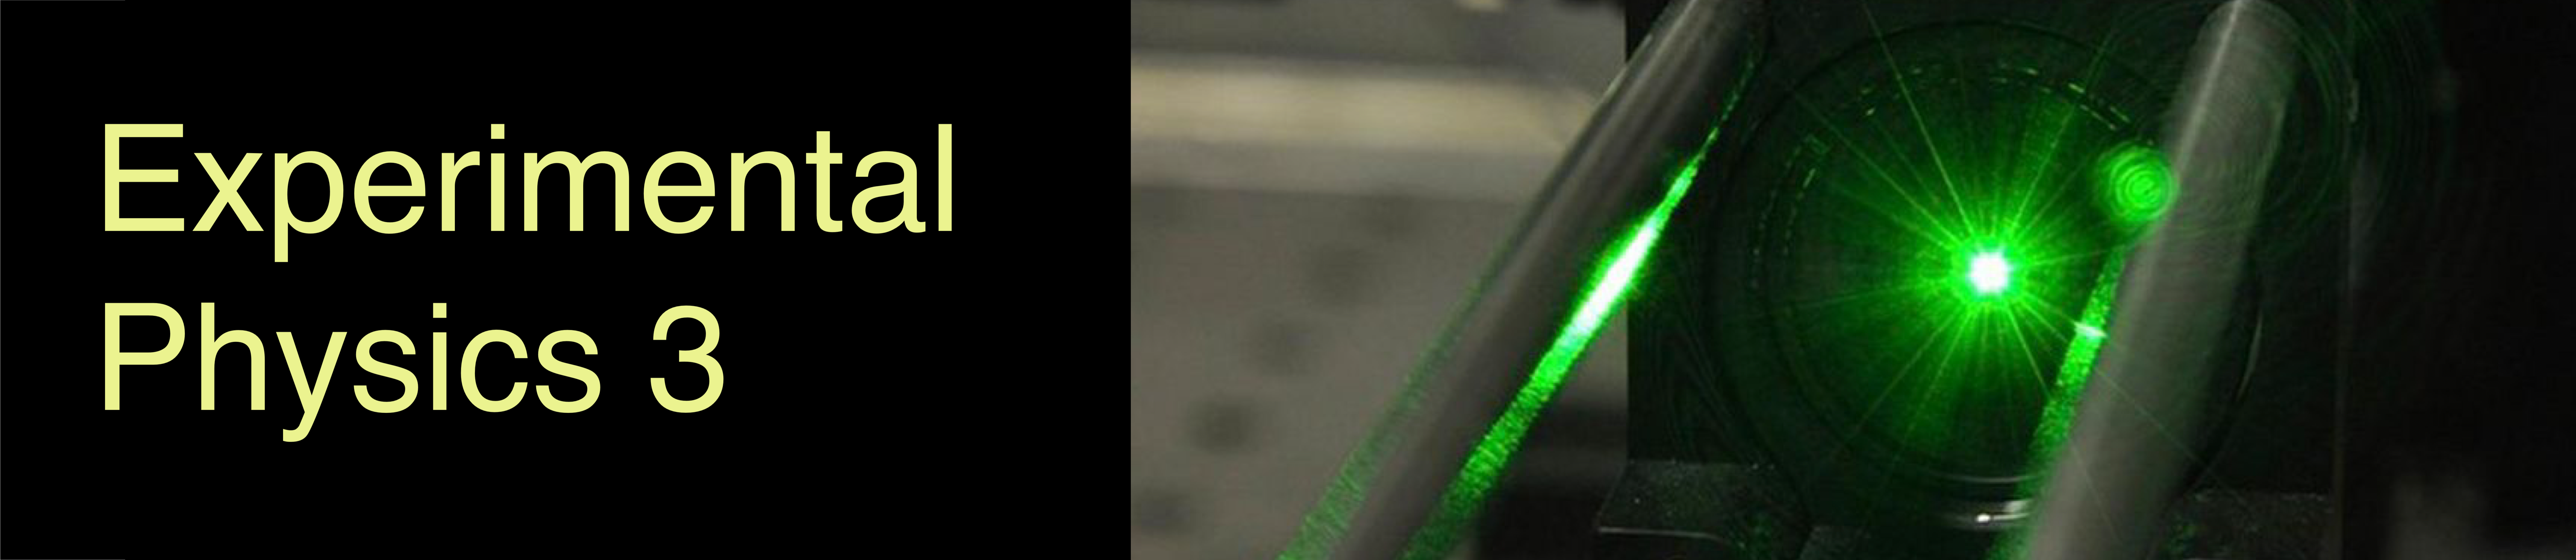
\includegraphics[keepaspectratio]{./assets/images/main/CompSoft_banner.png}}

\bookmarksetup{startatroot}

\chapter{Welcome to the Experimental Physics 3
Course!}\label{welcome-to-the-experimental-physics-3-course}

In this Experimental Physics 3 course, we will explore fundamental
experiments and mathematical descriptions related to light propagation,
electromagnetic waves, and their material counterpart, matter waves.
Specifically, we will focus on:

\begin{itemize}
\tightlist
\item
  Geometrical Optics
\item
  Wave Optics
\item
  Electromagnetic Waves
\item
  Matter Waves and Quantum Mechanics
\end{itemize}

The fields of optics and quantum mechanics are currently vibrant areas
of research, with rapidly evolving optical technologies, high-resolution
microscopy, and quantum information science. All of these advancements
build upon the foundations that we will address in this course.

\part{Geometrical Optics}

\chapter{Geometrical Optics}\label{geometrical-optics-1}

In this section, we will explore the fundamental principles that govern
how light behaves when it encounters different media and surfaces.

\section{\texorpdfstring{\textbf{Learning
Objectives}}{Learning Objectives}}\label{learning-objectives}

By the end of this section, you should be able to:

\begin{itemize}
\tightlist
\item
  Understand and apply the laws of reflection and refraction.
\item
  Analyze image formation by mirrors, lenses, and prisms.
\item
  Describe the working principles of various optical instruments.
\item
  Explain phenomena such as dispersion and imaging errors.
\end{itemize}

\section{\texorpdfstring{\textbf{Topics
Covered}}{Topics Covered}}\label{topics-covered}

\begin{enumerate}
\def\labelenumi{\arabic{enumi}.}
\item
  \textbf{\href{reflection.qmd}{Reflection}} Explore how light reflects
  off surfaces following the law of reflection.
\item
  \textbf{\href{refraction-total-internal-reflection.qmd}{Refraction and
  Total Internal Reflection}} Understand how light bends when passing
  through different media and the conditions for total internal
  reflection.
\item
  \textbf{\href{Optical\%20Elements\%20I.qmd}{Mirrors},\href{Optical\%20Elements\%20II.qmd}{Prisms}
  and \href{Optical\%20Elements\%20III.qmd}{Lenses} } Learn about
  various optical elements and how they form images.
\item
  \textbf{Optical Instruments} Study devices like telescopes and
  microscopes that utilize mirrors and lenses.
\item
  \textbf{Dispersion} Discover how different wavelengths of light
  refract differently, leading to phenomena like rainbows.
\item
  \textbf{Imaging Errors} Examine common aberrations in optical systems
  and methods to correct them.
\end{enumerate}

\section{\texorpdfstring{\textbf{Introduction}}{Introduction}}\label{introduction}

Geometrical optics is an approximate description of light propagation in
the limit of infinitely small wavelength, where all wave phenomena like
diffraction can be neglected.

\begin{figure}

{\centering \includegraphics[width=1\linewidth,height=\textheight,keepaspectratio]{geometrical-optics/img/geometrical-optics-intro.png}

}

\caption{Light rays passing through a lens system generated with
\href{https://benedikt-bitterli.me/tantalum/tantalum.html}{Tantalum}}

\end{figure}%

Light interacts with materials in predictable ways, allowing us to
design optical systems for imaging, magnification, and more.

\section{Assumptions of Geometrical
Optics}\label{assumptions-of-geometrical-optics}

Geometrical optics provides an approximate description of light behavior
and is based on several key assumptions. These assumptions simplify the
complex nature of light while still allowing for accurate predictions in
many practical scenarios.

\begin{tcolorbox}[enhanced jigsaw, coltitle=black, title=\textcolor{quarto-callout-note-color}{\faInfo}\hspace{0.5em}{Core Assumptions}, colframe=quarto-callout-note-color-frame, toprule=.15mm, opacitybacktitle=0.6, left=2mm, opacityback=0, breakable, toptitle=1mm, bottomtitle=1mm, leftrule=.75mm, arc=.35mm, titlerule=0mm, colbacktitle=quarto-callout-note-color!10!white, rightrule=.15mm, bottomrule=.15mm, colback=white]

\begin{enumerate}
\def\labelenumi{\arabic{enumi}.}
\tightlist
\item
  \textbf{Light Sources and Detection:}

  \begin{itemize}
  \tightlist
  \item
    Light rays emerge from a light source
  \item
    Light rays are detected by a detector
  \end{itemize}
\item
  \textbf{Light-Matter Interaction:}

  \begin{itemize}
  \tightlist
  \item
    Interaction is characterized by a refractive index \(n\)
  \item
    The speed of light in a medium is given by \(c=c_0/n\), where
    \(c_0\) is the speed of light in vacuum
  \item
    The speed in vacuum is \textbf{299.792.458 m/s} and is connected to
    the definition of the meter
  \end{itemize}
\item
  \textbf{Light Propagation:}

  \begin{itemize}
  \tightlist
  \item
    Light propagates in straight line paths (rays) in a homogeneous
    medium
  \item
    Light bends to a curved path in inhomogeneous media with varying
    refractive index \(n(\textbf{r})\)
  \end{itemize}
\item
  \textbf{Behavior at Interfaces:}

  \begin{itemize}
  \tightlist
  \item
    Rays may be reflected and refracted at interfaces between media
  \end{itemize}
\end{enumerate}

These assumptions form the foundation for understanding and predicting
light behavior in the context of geometrical optics.

\end{tcolorbox}

\chapter{Reflection}\label{reflection}

\begin{tcolorbox}[enhanced jigsaw, coltitle=black, title=\textcolor{quarto-callout-note-color}{\faInfo}\hspace{0.5em}{Historical Context of Reflection Laws}, colframe=quarto-callout-note-color-frame, toprule=.15mm, opacitybacktitle=0.6, left=2mm, opacityback=0, breakable, toptitle=1mm, bottomtitle=1mm, leftrule=.75mm, arc=.35mm, titlerule=0mm, colbacktitle=quarto-callout-note-color!10!white, rightrule=.15mm, bottomrule=.15mm, colback=white]

The study of reflection has a rich history dating back to ancient times:

\begin{enumerate}
\def\labelenumi{\arabic{enumi}.}
\item
  \textbf{Ancient Greece (300 BCE)}: Euclid, in his work ``Catoptrics,''
  was among the first to formally describe the law of reflection. He
  stated that the angle of incidence equals the angle of reflection.
\item
  \textbf{Ancient Rome (50 CE)}: Hero of Alexandria expanded on Euclid's
  work, applying the principle that light travels along the path of
  least distance.
\item
  \textbf{Islamic Golden Age (1000 CE)}: Ibn al-Haytham (Alhazen) made
  significant contributions to optics in his ``Book of Optics.'' He
  conducted experiments to verify the law of reflection and explored the
  properties of spherical and parabolic mirrors.
\item
  \textbf{17th Century}: Fermat's Principle, formulated by Pierre de
  Fermat, provided a more general framework for understanding reflection
  (and refraction) based on the principle of least time.
\item
  \textbf{Modern Era}: The understanding of reflection has been further
  refined with the development of electromagnetic theory by James Clerk
  Maxwell in the 19th century and quantum optics in the 20th century.
\end{enumerate}

\end{tcolorbox}

The law of reflection is probably the most simple one. Yet the
simplicity gives us the chance to define some basic objects which we
will further use for the description of light rays and their
propagation.

\subsection{Law of Reflection}\label{sec-law-of-reflection}

The sketch below shows the reflection of an incoming light ray (red) on
an interface. This incoming light ray has an angle \(\theta_{1}\) with
the axis (dashed line), which is perpendicular to the reflecting
surface. As compared to X-ray diffraction, we measure the angle to the
normal of the surface and not to the surface itself.

\begin{figure}

\begin{minipage}{0.50\linewidth}

\centering{

\includegraphics[width=0.8\linewidth,height=\textheight,keepaspectratio]{geometrical-optics/../assets/images/reflection/reflection.png}

}

\subcaption{\label{fig-reflection-diagram}Law of reflection}

\end{minipage}%
%
\begin{minipage}{0.50\linewidth}

\centering{

\includegraphics[width=0.8\linewidth,height=\textheight,keepaspectratio]{geometrical-optics/../assets/images/reflection/reflection_law.png}

}

\subcaption{\label{fig-reflection-experiment}Experimental Demonstration}

\end{minipage}%

\caption{\label{fig-reflection}Figure~\ref{fig-reflection-diagram}
illustrates the law of reflection, while Figure
Figure~\ref{fig-reflection-experiment} shows an experimental
demonstration.}

\end{figure}%

Figure~\ref{fig-reflection-diagram} shows the reflection of an incoming
light ray (red) on an interface. This incoming light ray has an angle
\(\theta_{1}\) with the axis (dashed line), which is perpendicular to
the reflecting surface. As compared to X-ray diffraction, we measure the
angle to the normal of the surface and not to the surface itself.

The law of reflection tells us now, that the outgoing reflected ray is
now leaving the surface under an angle \(\theta_2=\theta_1\). So both
angles are the same for the reflection.

\begin{tcolorbox}[enhanced jigsaw, coltitle=black, title=\textcolor{quarto-callout-tip-color}{\faLightbulb}\hspace{0.5em}{Law of Reflection}, colframe=quarto-callout-tip-color-frame, toprule=.15mm, opacitybacktitle=0.6, left=2mm, opacityback=0, breakable, toptitle=1mm, bottomtitle=1mm, leftrule=.75mm, arc=.35mm, titlerule=0mm, colbacktitle=quarto-callout-tip-color!10!white, rightrule=.15mm, bottomrule=.15mm, colback=white]

If a ray is incident to a reflecting surface under an angle \(\theta_1\)
it will be reflected towards under an angle \(\theta_2=\theta_1\) to the
same side of the surface.

\end{tcolorbox}

\subsection{Fermat's Principle}\label{sec-fermat-principle}

The law of reflection can be actually obtained from a variational
principle saying the light rays propagate along those path on which the
propagation time is an extremum. This variational principle is called
Fermat's principle.

\begin{figure}

\centering{

\includegraphics[width=0.6\linewidth,height=\textheight,keepaspectratio]{geometrical-optics/../assets/images/reflection/fermat.png}

}

\caption{\label{fig-fermat}Sketch for deriving the law of reflection
from Fermat's principle}

\end{figure}%

Consider now a light ray that should travel from point \(A\) to point
\(C\) via a point \(B\) on the mirror surface. In general multiple paths
are possible such as the one indicated in the above picture. Clearly
this path is not satisfying our reflection law formulated above.
Fermat's principle now restricts the path length from \(A\) to \(C\) to
be the one, which takes the least amount of time.

\begin{tcolorbox}[enhanced jigsaw, coltitle=black, title=\textcolor{quarto-callout-tip-color}{\faLightbulb}\hspace{0.5em}{Fermat's principle}, colframe=quarto-callout-tip-color-frame, toprule=.15mm, opacitybacktitle=0.6, left=2mm, opacityback=0, breakable, toptitle=1mm, bottomtitle=1mm, leftrule=.75mm, arc=.35mm, titlerule=0mm, colbacktitle=quarto-callout-tip-color!10!white, rightrule=.15mm, bottomrule=.15mm, colback=white]

The path taken by a ray between two given points A, B is the path that
can be traversed in the least time.

\emph{More precise alternative:} A ray going in a certain particular
path has the property that if we make a small change in the ray in any
manner whatever, say in the location at which it comes to the mirror, or
the shape of the curve, or anything, there will be no first-order change
in the time; there will be only a second-order change in the time.

\end{tcolorbox}

So let us consider that contraints to the path length. The total length
the light hast to travel via the three points is

\[
l=l_{1}+l_{2}=\sqrt{(x-x_1)^2+y_1^2}+\sqrt{(x_2-x)^2+y_2^2}
\]

The time that is required by the light to travel that distance \(l\) is
then given by

\[
t=\frac{l}{c},
\]

where \(c\) is the speed of light in the medium above the mirror. If
this time should now be a minimum, we have to take the derivative of the
time \(t\) with respect to the position \(x\) on the mirror and set that
to zero, i.e.,

\begin{equation}\phantomsection\label{eq-hello}{\frac{\mathrm dt}{\mathrm dx}=0.}\end{equation}

This results in Equation~\ref{eq-hello}

\[
\frac{x-x_1}{\sqrt{(x-x_1)^2+y_{1}^2}}=\frac{x_2-x}{\sqrt{(x_2-x)^2+y_{2}^2}},
\]

which is actually

\[
\frac{x-x_1}{l_1}=\frac{x_2-x}{l_2}
\]

or

\[
\sin(\theta_1)=\sin(\theta_2)
\]

which finally requires

\[
\theta_1=\theta_2
\]

and is our law of reflection. Thus, reflection satisfies Fermat's
principle, i.e.~the light rays propagate along those path on which the
propagation time is an extremum.

\begin{tcolorbox}[enhanced jigsaw, coltitle=black, title=\textcolor{quarto-callout-tip-color}{\faLightbulb}\hspace{0.5em}{Principle of Least Action (Hamilton's Principle)}, colframe=quarto-callout-tip-color-frame, toprule=.15mm, opacitybacktitle=0.6, left=2mm, opacityback=0, breakable, toptitle=1mm, bottomtitle=1mm, leftrule=.75mm, arc=.35mm, titlerule=0mm, colbacktitle=quarto-callout-tip-color!10!white, rightrule=.15mm, bottomrule=.15mm, colback=white]

The Principle of Least Action, also known as Hamilton's Principle, is a
fundamental concept in classical mechanics. It states that the path
taken by a physical system between two states is the one for which the
action integral is stationary (usually a minimum).

\subsection{Action Integral}\label{action-integral}

The action \(S\) is defined as the integral of the Lagrangian \(L\) over
time:

\[
S = \int_{t_1}^{t_2} L \, dt
\]

\subsection{Lagrangian}\label{lagrangian}

The Lagrangian \(L\) is a function that summarizes the dynamics of the
system. For a system with generalized coordinates \(q_i\) and velocities
\(\dot{q}_i\), the Lagrangian is typically given by:

\[
L = T - V
\]

where:

\begin{itemize}
\item
  \(T\) is the kinetic energy of the system.
\item
  \(V\) is the potential energy of the system.
\end{itemize}

\subsection{Euler-Lagrange Equations}\label{euler-lagrange-equations}

Hamilton's Principle leads to the Euler-Lagrange equations, which are
the equations of motion for the system. These equations are derived by
requiring that the action \(S\) be stationary with respect to variations
in the path \(q_i(t)\):

\[
\delta S = 0
\]

This condition leads to the following differential equations:

\[
\frac{d}{dt} \left( \frac{\partial L}{\partial \dot{q}_i} \right) - \frac{\partial L}{\partial q_i} = 0
\]

These are the Euler-Lagrange equations, and they provide a powerful
method for deriving the equations of motion for a wide variety of
physical systems.

\subsection{Example: Simple Harmonic
Oscillator}\label{example-simple-harmonic-oscillator}

For a simple harmonic oscillator with mass \(m\) and spring constant
\(k\), the Lagrangian is:

\[
L = \frac{1}{2} m \dot{x}^2 - \frac{1}{2} k x^2
\]

Applying the Euler-Lagrange equation:

\[
\frac{d}{dt} \left( \frac{\partial L}{\partial \dot{x}} \right) - \frac{\partial L}{\partial x} = 0
\]

we get:

\[
m \ddot{x} + k x = 0
\]

which is the familiar equation of motion for a simple harmonic
oscillator.

Hamilton's Principle and the associated Euler-Lagrange equations are
foundational in classical mechanics and have far-reaching implications
in other areas of physics, including quantum mechanics and field theory.

\end{tcolorbox}

\chapter{Refraction and Total Internal
Reflection}\label{refraction-and-total-internal-reflection}

\section{Refraction}\label{refraction}

\begin{tcolorbox}[enhanced jigsaw, coltitle=black, title=\textcolor{quarto-callout-note-color}{\faInfo}\hspace{0.5em}{Historical Context of Refraction}, colframe=quarto-callout-note-color-frame, toprule=.15mm, opacitybacktitle=0.6, left=2mm, opacityback=0, breakable, toptitle=1mm, bottomtitle=1mm, leftrule=.75mm, arc=.35mm, titlerule=0mm, colbacktitle=quarto-callout-note-color!10!white, rightrule=.15mm, bottomrule=.15mm, colback=white]

The understanding of refraction has evolved over centuries, with
contributions from various cultures and scientific traditions. This
timeline highlights key milestones in the discovery and formalization of
refraction, showcasing how our comprehension of this fundamental optical
phenomenon has deepened over time:

\begin{enumerate}
\def\labelenumi{\arabic{enumi}.}
\item
  \textbf{Ancient Greece (3rd century BCE):} Euclid noticed that a stick
  partially submerged in water appears bent. Archimedes studied the
  refraction of light in water.
\item
  \textbf{Ancient Rome (1st century CE):} Ptolemy conducted experiments
  on refraction and compiled tables of refraction angles for different
  media.
\item
  \textbf{Islamic Golden Age (10th-11th centuries):} Ibn Sahl (940-1000)
  discovered the law of refraction, describing it geometrically. Alhazen
  (965-1040) studied lenses and the human eye, contributing
  significantly to optics.
\item
  \textbf{Middle Ages:} Robert Grosseteste (1175-1253) and Roger Bacon
  (1214-1294) studied refraction and its application to lenses.
\item
  \textbf{Renaissance:} Thomas Harriot (1560-1621) rediscovered the law
  of refraction but didn't publish his findings.
\item
  \textbf{17th Century:} Willebrord Snellius (1580-1626) derived the
  mathematical law of refraction (Snell's law) around 1621. René
  Descartes (1596-1650) independently derived and published the law of
  refraction in 1637. Pierre de Fermat (1607-1665) derived the law of
  refraction using his principle of least time.
\item
  \textbf{19th Century:} Augustin-Jean Fresnel (1788-1827) developed the
  wave theory of light, explaining refraction in terms of changes in
  wave speed.
\item
  \textbf{20th Century:} The quantum mechanical understanding of light,
  which emerged in the early 20th century, significantly impacted our
  view of refraction. Max Planck's work on black body radiation in 1900
  and Albert Einstein's explanation of the photoelectric effect in 1905
  laid the groundwork for the quantum nature of light. This quantum
  perspective provided a complementary explanation to the wave theory,
  describing refraction in terms of photons interacting with the atoms
  in the medium. While this quantum view offers insights into certain
  aspects of refraction, it's important to note that both the wave and
  particle descriptions of light are necessary for a complete
  understanding of optical phenomena.
\end{enumerate}

\end{tcolorbox}

The law of refraction is the second important law of geometrical optics.
It relates the refractive index \(n_1\) and angle of incidence
\(\theta_1\) on one side of an interface to the refractive index \(n_2\)
and angle of refraction \(\theta_2\) on the other side. Both the law of
reflection and the law of refraction can be derived from more
fundamental principles such as Fermat's principle of least time and are
consistent with the conservation of energy. Their relation to momentum
is more complex and involves considering the interaction of light with
the medium at an atomic level. These laws provide a mathematical
framework for predicting how light behaves when it encounters interfaces
between different media, forming the basis for understanding a wide
range of optical phenomena and the design of optical devices.

\subsection{Refractive Index}\label{refractive-index}

The refractive index \(n\) is a material constant representing the
factor by which the speed of light is reduced in the medium compared to
its speed in vacuum. For most natural materials and visible light, the
refractive index is \(n \ge 1\), as light typically travels slower in
media than in vacuum. However, in certain special cases---such as for
X-rays in some materials or in engineered metamaterials---the refractive
index can be less than 1 or even negative. Understanding these exotic
cases requires a deeper exploration of the electromagnetic properties of
materials and the origin of the refractive index, which we will address
later.

\subsection{Snells Law}\label{snells-law}

\includegraphics[width=0.59\linewidth,height=\textheight,keepaspectratio]{geometrical-optics/../assets/images/reflection/snell.png}
\begin{center}
\includegraphics[width=0.4\linewidth,height=\textheight,keepaspectratio]{geometrical-optics/../assets/images/reflection/refraction_law.png}
\end{center}

\begin{tcolorbox}[enhanced jigsaw, coltitle=black, title=\textcolor{quarto-callout-tip-color}{\faLightbulb}\hspace{0.5em}{Law of Refraction (Snell's Law)}, colframe=quarto-callout-tip-color-frame, toprule=.15mm, opacitybacktitle=0.6, left=2mm, opacityback=0, breakable, toptitle=1mm, bottomtitle=1mm, leftrule=.75mm, arc=.35mm, titlerule=0mm, colbacktitle=quarto-callout-tip-color!10!white, rightrule=.15mm, bottomrule=.15mm, colback=white]

The law of refraction (Snell's law) is given for the above sketch by the
equation:

\[
n_1 \sin(\theta_1)=n_2 \sin(\theta_2)
\]

\end{tcolorbox}

You can explore the law of refraction using the interactive
visualization below. The visualization shows a light ray incident on an
interface between two media with different refractive indices. You can
adjust the angle of incidence and the refractive index of the first
medium to see how the angle of refraction changes according to Snell's
law.

Snell's law leads to some general patterns in the behavior of light rays
at interfaces, which are worth remembering. Consider these two cases:

\begin{enumerate}
\def\labelenumi{\arabic{enumi}.}
\tightlist
\item
  When light moves from a medium with lower refractive index to one with
  higher refractive index (\(n_1 < n_2\)):

  \begin{itemize}
  \tightlist
  \item
    The refracted ray bends towards the normal (optical axis)
  \item
    The angle of refraction is smaller than the angle of incidence
    (\(\theta_2 < \theta_1\))
  \end{itemize}
\item
  When light moves from a medium with higher refractive index to one
  with lower refractive index (\(n_1 > n_2\)):

  \begin{itemize}
  \tightlist
  \item
    The refracted ray bends away from the normal (optical axis)
  \item
    The angle of refraction is larger than the angle of incidence
    (\(\theta_2 > \theta_1\))
  \end{itemize}
\end{enumerate}

Figure Figure~\ref{fig-snells-combinations} illustrates these principles
with three plots showing how the refracted angle changes with the
incident angle for two common interface scenarios: glass-to-air and
air-to-glass. These plots clearly demonstrate the different behaviors
described above.

\begin{figure}

\centering{

\pandocbounded{\includegraphics[keepaspectratio]{geometrical-optics/refraction-total-internal-reflection_files/figure-pdf/fig-snells-combinations-output-1.pdf}}

}

\caption{\label{fig-snells-combinations}Snell's law for different
combinations of refractive indices. The plots show the relationship
between incident angle (\(\theta_1\)) and refracted angle (\(\theta_2\))
for three scenarios: (a) light passing from air to glass, (b) light
passing from glass to air, and (c) a comparison of both cases. Note how
the curves differ when light moves into a medium with higher refractive
index versus a lower refractive index.}

\end{figure}%

\subsection{Total Internal Reflection}\label{total-internal-reflection}

The above diagram reveals a special case occurring when \(n_1 > n_2\).
Under these conditions, we can increase the incident angle \(\theta_1\)
until the outgoing angle reaches \(\theta_2 = \frac{\pi}{2}\). At this
point, the refracted ray would be traveling along the interface between
the two media. For any incident angle \(\theta_1\) larger than this
critical angle, there is no refracted ray at all; instead, we observe
only a reflected ray. This phenomenon, known as \textbf{total internal
reflection}, occurs despite the fact that the material with refractive
index \(n_2\) is completely transparent.

Let's formalize this concept mathematically. Using Snell's law and
setting \(\theta_2 = \frac{\pi}{2}\), we obtain the equation for the
critical angle \(\theta_c\):

\[\theta_1 = \theta_c = \sin^{-1}\left(\frac{n_2}{n_1}\right)\]

Note that the \(\sin^{-1}()\) function requires an argument \(\le 1\),
which is why this phenomenon only occurs when \(n_2 < n_1\).

It's important to understand that during total internal reflection, all
of the light energy is reflected back into the first medium, hence the
term `total'. However, electromagnetic optics reveals an interesting
subtlety: an evanescent wave penetrates a short distance into the second
medium, though it doesn't propagate energy across the boundary.

When the incident angle exceeds the critical angle, Snell's law as we've
written it no longer applies. Instead, we observe perfect reflection,
where the angle of reflection equals the angle of incidence, just as in
regular reflection from a mirror. This reflection occurs without any
loss of energy to the second medium, making it an extremely efficient
process.

\includegraphics[width=0.5\linewidth,height=\textheight,keepaspectratio]{geometrical-optics/../assets/images/reflection/tir.png}
\begin{center}
\includegraphics[width=0.49\linewidth,height=\textheight,keepaspectratio]{geometrical-optics/../assets/images/reflection/tir_disk.png}
\end{center}

\begin{tcolorbox}[enhanced jigsaw, coltitle=black, title=\textcolor{quarto-callout-tip-color}{\faLightbulb}\hspace{0.5em}{Total Internal Reflection}, colframe=quarto-callout-tip-color-frame, toprule=.15mm, opacitybacktitle=0.6, left=2mm, opacityback=0, breakable, toptitle=1mm, bottomtitle=1mm, leftrule=.75mm, arc=.35mm, titlerule=0mm, colbacktitle=quarto-callout-tip-color!10!white, rightrule=.15mm, bottomrule=.15mm, colback=white]

Total internal reflection occurs when light is passing from higher
refractive index to lower refractive index materials for incidence angle
larger than a critical angle

\[
\theta_c=\sin^{-1}\left (\frac{n_2}{n_1}\right )
\]

\end{tcolorbox}

We can demonstrate total internal reflection very easily with a water
basin, for example, where we couple in light from a laser from the side.

\includegraphics[width=0.59\linewidth,height=\textheight,keepaspectratio]{geometrical-optics/../assets/images/reflection/basin_tir.png}
\begin{center}
\includegraphics[width=0.4\linewidth,height=\textheight,keepaspectratio]{geometrical-optics/../assets/images/reflection/tir_basin.png}
\end{center}

But you could try that yourself also in the bath tub diving below the
water surface.

Total internal reflection has numerous practical applications:

\begin{enumerate}
\def\labelenumi{\arabic{enumi}.}
\tightlist
\item
  Fiber optic communications: Light signals can travel long distances
  with minimal loss through optical fibers.
\item
  Optical instruments: Prisms in binoculars and telescopes use total
  internal reflection to manipulate light paths.
\item
  Gemstones: The sparkle of diamonds is enhanced by total internal
  reflection trapping light within the stone.
\item
  Medical endoscopes: Total internal reflection helps guide light
  through flexible tubes for internal imaging.
\end{enumerate}

\textbf{Optical Fibers and Total Internal Reflection}

Total internal reflection plays a crucial role in modern
telecommunications, particularly in optical fibers, which are also part
of many experimental setups. These fibers are essentially ultra-thin
glass wires, ranging in diameter from a few micrometers to several
hundred micrometers, designed to transport light over long distances
with minimal loss.

The structure of an optical fiber is key to its function:

\begin{enumerate}
\def\labelenumi{\arabic{enumi}.}
\tightlist
\item
  Core: A central glass core with a refractive index \(n_1\)
\item
  Cladding: A surrounding layer with a slightly lower refractive index
  \(n_2\)
\end{enumerate}

This difference in refractive indices is what allows total internal
reflection to occur within the fiber.

\includegraphics[width=0.59\linewidth,height=\textheight,keepaspectratio]{geometrical-optics/../assets/images/reflection/fiber.png}
\begin{center}
\includegraphics[width=0.4\linewidth,height=\textheight,keepaspectratio]{geometrical-optics/../assets/images/reflection/tir_rod.png}
\end{center}

For light to propagate effectively through the fiber, it must enter at
an angle that ensures total internal reflection at the core-cladding
interface. This leads to the concept of the acceptance angle,
\(\theta_a\), which is the maximum angle at which light can enter the
fiber and still undergo total internal reflection.

To characterize this acceptance angle, optical engineers use a parameter
called the \textbf{Numerical Aperture (NA)}.

\begin{tcolorbox}[enhanced jigsaw, coltitle=black, title=\textcolor{quarto-callout-tip-color}{\faLightbulb}\hspace{0.5em}{Numerical Aperture}, colframe=quarto-callout-tip-color-frame, toprule=.15mm, opacitybacktitle=0.6, left=2mm, opacityback=0, breakable, toptitle=1mm, bottomtitle=1mm, leftrule=.75mm, arc=.35mm, titlerule=0mm, colbacktitle=quarto-callout-tip-color!10!white, rightrule=.15mm, bottomrule=.15mm, colback=white]

The Numerical Aperture of a fiber is defined as the sine of the maximum
acceptance angle:

\begin{equation}
NA = \sin(\theta_a) = \sqrt{n_1^2 - n_2^2}
\end{equation}

\end{tcolorbox}

This equation relates the NA directly to the refractive indices of the
core and cladding. The derivation of this formula involves applying
Snell's law at the air-fiber interface and at the core-cladding
interface, then using the condition for total internal reflection.

In practice, typical values for the refractive indices might be
\(n_1 = 1.475\) for the core and \(n_2 = 1.46\) for the cladding.
Plugging these into our equation:

\begin{equation}
NA = \sqrt{1.475^2 - 1.46^2} \approx 0.2
\end{equation}

This means that light entering the fiber within a cone of about 11.5°
(arcsin(0.2)) from the fiber's axis will be transmitted through the
fiber via total internal reflection.

The NA is an important parameter in fiber optic design:

\begin{enumerate}
\def\labelenumi{\arabic{enumi}.}
\tightlist
\item
  It determines the light-gathering ability of the fiber.
\item
  It affects the fiber's bandwidth and its susceptibility to certain
  types of signal distortion.
\item
  It influences how easily the fiber can be coupled to light sources and
  other fibers.
\end{enumerate}

Optical fibers come in various types, each optimized for different
applications. Some fibers are designed to transmit light over long
distances with minimal loss, while others are engineered for specific
wavelengths or to guide light in unusual ways. The figure below shows a
few examples of optical fiber types.

\begin{figure}

\centering{

\includegraphics[width=1\linewidth,height=\textheight,keepaspectratio]{geometrical-optics/img/fibers.png}

}

\caption{\label{fig-optical-fiber}Rendering of different optical fibers
types (from left to right): Hollow core optical fiber, hollow core bragg
fiber, photonic crystal fiber, conventional fiber}

\end{figure}%

\subsection{Fermat's Principle for Inhomogeneous
Media}\label{fermats-principle-for-inhomogeneous-media}

While before we have considered Fermat's principle for the special case
of refraction and light propagation in a homogeneous medium, we can
define a more general version of it correponding to the following
situation also involving an inhomogeneous refractive index
\(n(\vec{r})\).

\begin{figure}

\centering{

\includegraphics[width=0.4\linewidth,height=\textheight,keepaspectratio]{geometrical-optics/../assets/images/reflection/fermat_general.png}

}

\caption{\label{fig-fermat-general}Sketch for a general description of
Fermat's principle}

\end{figure}%

For this general scenario of light traveling along a path, we can define
an optical path length (OPL) as

\begin{equation}
\text{OPL} = \int\limits_{A}^{C} n(\mathbf{r}) \mathrm ds=0,
\end{equation}

with a varying refractive index \(n(\mathbf{r})\). Fermat's Principle
states that the actual path taken by the light makes the OPL stationary:

\[
\delta \left( \int_A^B n(\mathbf{r}) \, ds \right) = 0
\]

Using the calculus of variations, this leads to the Euler-Lagrange
equation for the path of light. In Cartesian coordinates, if the path is
parameterized by \(\mathbf{r}(s) = (x(s), y(s), z(s))\), the
Euler-Lagrange equations become:

\[
\frac{d}{ds} \left( n \frac{d\mathbf{r}}{ds} \right) = \nabla n
\]

where \(\nabla n\) is the gradient of the refractive index. This
equation describes how the light ray bends in response to changes in the
refractive index of the medium.

Fermat's Principle is a cornerstone of geometrical optics and has
applications in designing optical systems, understanding mirages, and
analyzing the behavior of light in various media.

\begin{tcolorbox}[enhanced jigsaw, coltitle=black, title=\textcolor{quarto-callout-tip-color}{\faLightbulb}\hspace{0.5em}{Fermat's Principle and Snells Law}, colframe=quarto-callout-tip-color-frame, toprule=.15mm, opacitybacktitle=0.6, left=2mm, opacityback=0, breakable, toptitle=1mm, bottomtitle=1mm, leftrule=.75mm, arc=.35mm, titlerule=0mm, colbacktitle=quarto-callout-tip-color!10!white, rightrule=.15mm, bottomrule=.15mm, colback=white]

We would like to apply Fermat's principle to derive Snell's law, which
is a more lengthy calculation. To do this, we consider a light ray
traveling from point \(A\) in medium 1 (with refractive index \(n_1\))
to point \(C\) in medium 2 (with refractive index \(n_2\)), crossing the
interface at point \(B\). Let the coordinates of points \(A\), \(B\),
and \(C\) be \((x_A, y_A)\), \((x_B, y_B)\), and \((x_C, y_C)\),
respectively. Assume the interface between the two media is at
\(y = y_B\). The optical path length (OPL) is given by:

\[
\delta \int_{A}^{C} n(\vec{r}) \, ds = 0,
\]

where \(n(\vec{r})\) is the refractive index at position \(\vec{r}\),
and \(ds\) is an infinitesimal element of the path.

Consider a light ray traveling from point \(A\) in medium 1 (with
refractive index \(n_1\)) to point \(C\) in medium 2 (with refractive
index \(n_2\)), crossing the interface at point \(B\). Let the
coordinates of points \(A\), \(B\), and \(C\) be \((x_A, y_A)\),
\((x_B, y_B)\), and \((x_C, y_C)\), respectively. Assume the interface
between the two media is at \(y = y_B\).

\subsubsection{Optical Path Length}\label{optical-path-length}

The optical path length (OPL) is given by:

\[
\text{OPL} = n_1 \int_{A}^{B} ds_1 + n_2 \int_{B}^{C} ds_2,
\]

where \(ds_1\) and \(ds_2\) are the infinitesimal path lengths in media
1 and 2, respectively.

\subsubsection{Path Lengths}\label{path-lengths}

The path lengths \(ds_1\) and \(ds_2\) can be expressed in terms of the
coordinates:

\[
ds_1 = \sqrt{(dx_1)^2 + (dy_1)^2}, \quad ds_2 = \sqrt{(dx_2)^2 + (dy_2)^2}.
\]

Since the interface is at \(y = y_B\), we have \(dy_1 = y_B - y_A\) and
\(dy_2 = y_C - y_B\). The total optical path length is:

\[
\text{OPL} = n_1 \sqrt{(x_B - x_A)^2 + (y_B - y_A)^2} + n_2 \sqrt{(x_C - x_B)^2 + (y_C - y_B)^2}.
\]

\subsubsection{Applying Fermat's
Principle}\label{applying-fermats-principle}

To find the stationary path, we take the variation of the OPL with
respect to \(x_B\):

\[
\delta \text{OPL} = \delta \left[ n_1 \sqrt{(x_B - x_A)^2 + (y_B - y_A)^2} + n_2 \sqrt{(x_C - x_B)^2 + (y_C - y_B)^2} \right] = 0.
\]

Taking the derivative with respect to \(x_B\):

\[
\frac{\partial}{\partial x_B} \left[ n_1 \sqrt{(x_B - x_A)^2 + (y_B - y_A)^2} + n_2 \sqrt{(x_C - x_B)^2 + (y_C - y_B)^2} \right] = 0.
\]

\subsubsection{Differentiating}\label{differentiating}

Differentiating each term separately:

\[
n_1 \frac{\partial}{\partial x_B} \sqrt{(x_B - x_A)^2 + (y_B - y_A)^2} + n_2 \frac{\partial}{\partial x_B} \sqrt{(x_C - x_B)^2 + (y_C - y_B)^2} = 0.
\]

Using the chain rule:

\[
n_1 \frac{x_B - x_A}{\sqrt{(x_B - x_A)^2 + (y_B - y_A)^2}} + n_2 \frac{x_B - x_C}{\sqrt{(x_C - x_B)^2 + (y_C - y_B)^2}} = 0.
\]

\subsubsection{Simplifying}\label{simplifying}

Let \(\theta_1\) be the angle of incidence and \(\theta_2\) be the angle
of refraction. Then:

\[
\sin \theta_1 = \frac{x_B - x_A}{\sqrt{(x_B - x_A)^2 + (y_B - y_A)^2}}, \quad \sin \theta_2 = \frac{x_C - x_B}{\sqrt{(x_C - x_B)^2 + (y_C - y_B)^2}}.
\]

Substituting these into the equation:

\[
n_1 \sin \theta_1 + n_2 \sin \theta_2 = 0.
\]

Since \(\sin \theta_2\) is in the opposite direction, we have:

\[
n_1 \sin \theta_1 = n_2 \sin \theta_2.
\]

This is Snell's law, which describes the relationship between the angles
of incidence and refraction when light passes from one medium to
another.

\subsubsection{Conclusion}\label{conclusion}

By applying Fermat's principle and taking the variation of the optical
path length, we have derived Snell's law:

\[
n_1 \sin \theta_1 = n_2 \sin \theta_2.
\]

This demonstrates how the principle of least time leads to the
well-known law of refraction in optics.

\end{tcolorbox}

\begin{tcolorbox}[enhanced jigsaw, coltitle=black, title=\textcolor{quarto-callout-tip-color}{\faLightbulb}\hspace{0.5em}{Example: Light in a Graded-Index Medium}, colframe=quarto-callout-tip-color-frame, toprule=.15mm, opacitybacktitle=0.6, left=2mm, opacityback=0, breakable, toptitle=1mm, bottomtitle=1mm, leftrule=.75mm, arc=.35mm, titlerule=0mm, colbacktitle=quarto-callout-tip-color!10!white, rightrule=.15mm, bottomrule=.15mm, colback=white]

Consider a medium where the refractive index varies with height \(y\) as
\(n(y) = n_0 (1 - \frac{\alpha^2}{2 n_0} y^2)\). The path of light in
such a medium can be found by using Fermat's principle in differential
form:

\[
\frac{d}{ds}\left (n(\textbf{r})\frac{d\textbf{r}}{ds}\right)=\nabla n(\textbf{r})
\]

Typically, this requires to express the coordinates in terms of a
parameter, such as \(x(s)\) and \(y(s)\), and then solve the
differential equation. The solution will give the path of light in the
medium. This is difficult and commonly done numerically. In paraxial
optics, when the light is propagating roughly in the direction of \(z\),
the differential element \(ds\) can be approximated as \(dz\) since then

\[
ds=dz\sqrt{1+\left (\frac{dy}{dz}\right )^2+\left (\frac{dx}{dz}\right)^2}\approx dz
\]

which yields

\[
\frac{d}{dz}\left (n\frac{dx}{dz}\right)\approx \frac{dn}{dx}
\]

and

\[
\frac{d}{dz}\left (n\frac{dy}{dz}\right )\approx \frac{dn}{dy}
\]

This readily yields the path of light in a homogeneous medium, where
\(n\) is constant. In this case we have

\[
\frac{d^2 x}{dz^2}=\frac{d^2 y}{dz^2}=0
\]

which is true for a straight line. In a graded-index medium, the path of
light can be found by solving the differential equation

\[
\frac{d^2 y}{dz^2}=-\alpha^2 y
\]

which is reminiscent of the equation of motion of a harmonic oscillator.
The solution is therefore an oscillating function

\[
y(z)=y_0\cos(\alpha z)+\frac{\theta_0}{\alpha}\sin(\alpha z  )
\]

where the angle \(\theta_0\) is the initial angle of the light ray with
respect to the \(z\) axis. This solution describes the path of light in
a graded-index medium.

\end{tcolorbox}

\begin{tcolorbox}[enhanced jigsaw, coltitle=black, title=\textcolor{quarto-callout-tip-color}{\faLightbulb}\hspace{0.5em}{Fermats's Principle in Integral and Differential Form}, colframe=quarto-callout-tip-color-frame, toprule=.15mm, opacitybacktitle=0.6, left=2mm, opacityback=0, breakable, toptitle=1mm, bottomtitle=1mm, leftrule=.75mm, arc=.35mm, titlerule=0mm, colbacktitle=quarto-callout-tip-color!10!white, rightrule=.15mm, bottomrule=.15mm, colback=white]

We have described Fermat't principle in an integral form specifiying the
optical path length \(S\) as

\[
OPL=\int n(\textbf{r})ds
\]

The path length \(ds\) can be given in terms of two coordinates \(x_1\)
and \(x_2\) parametrized by \(\lambda\) such that

\[
ds=\sqrt{\dot{x}_1^{2}+\dot{x}_2^{2}}d\lambda
\]

where \(\dot{x}_1=\frac{dx_{1}}{d\lambda}\). We can therefore write
Fermat's principle as

\[
\delta OPL=\int\left[\left(\frac{\partial n}{\partial x_i} \delta x_i\right) \sqrt{\dot{x}_1^2+\dot{x}_2^2}+n \frac{1}{\sqrt{\dot{x}_1^2+\dot{x}_2^2}} \dot{x}_i \delta \dot{x}_i\right] d \lambda = 0
\]

To evaluate this integral we would like to integrate by parts. We can
write the integrand as \[
u = n \frac{1}{\sqrt{\dot{x}_1^2+\dot{x}_2^2}} \dot{x}_i
\]

and

\[
dv = \delta \dot{x}_i d\lambda
\]

We can now calculate \(du\) and \(v\) and obtain

\[
du = \frac{d}{d\lambda}\left[n \frac{1}{\sqrt{\dot{x}_1^2+\dot{x}_2^2}} \dot{x}_i\right] d\lambda
\]

and

\[
v = \delta x_i
\]

With these expressions we can now apply the integration by parts formula
\(\int u dv = uv - \int v du\), we get:

\[
\int n \frac{1}{\sqrt{\dot{x}_1^2+\dot{x}_2^2}} \dot{x}_i \delta \dot{x}_i d\lambda = \left[n \frac{1}{\sqrt{\dot{x}_1^2+\dot{x}_2^2}} \dot{x}_i \delta x_i\right]|_{\lambda_1}^{\lambda_2} - \int \delta x_i \frac{d}{d\lambda}\left[n \frac{1}{\sqrt{\dot{x}_1^2+\dot{x}_2^2}} \dot{x}_i\right] d\lambda
\]

This can be substituted back into the original equation to obtain

\[
\begin{aligned}
\delta OPL &= \int \left[\left(\frac{\partial n}{\partial x_i} \delta x_i\right) \sqrt{\dot{x}_1^2+\dot{x}_2^2}\right] d\lambda \\
&+ \left[n \frac{1}{\sqrt{\dot{x}_1^2+\dot{x}_2^2}} \dot{x}_i \delta x_i\right]|_{\lambda_1}^{\lambda_2} \\
&- \int \delta x_i \frac{d}{d\lambda}\left[n \frac{1}{\sqrt{\dot{x}_1^2+\dot{x}_2^2}} \dot{x}_i\right] d\lambda = 0
\end{aligned}
\]

After rearranging the terms we get

\[
\begin{aligned}
\delta OPL &= \int \left\{\frac{\partial n}{\partial x_i} \sqrt{\dot{x}_1^2+\dot{x}_2^2} - \frac{d}{d\lambda}\left[n \frac{1}{\sqrt{\dot{x}_1^2+\dot{x}_2^2}} \dot{x}_i\right]\right\} \delta x_i d\lambda \\
&+ \left[n \frac{1}{\sqrt{\dot{x}_1^2+\dot{x}_2^2}} \dot{x}_i \delta x_i\right]|_{\lambda_1}^{\lambda_2} = 0
\end{aligned}
\]

and therefore finally

\[
\delta OPL=\int\left[\left(\frac{\partial n}{\partial x_i}\right) \sqrt{\dot{x}_1{ }^2+\dot{x}_2{ }^2}-\frac{d}{d \lambda}\left(n \frac{1}{\sqrt{\dot{x}_1^2+\dot{x}_2^2}} \dot{x}_i\right)\right] \delta x_i d \lambda+\text { boundary terms }
\]

for which we choose the parameter \(\lambda\) such that the boundary
terms vanish.

\[
\lambda=s
\]

such that

\[
\sqrt{\dot{x}_1^2+\dot{x}_2^2}=1
\]

and finally leads to the Euler-Lagrange equation

\[
\left(\frac{\partial n}{\partial x_i}\right)-\frac{d}{d s}\left(n \dot{x}_i\right)=0
\]

which is the differential form of the Fermat's principle.

\end{tcolorbox}

\chapter{Optical Elements Part I}\label{optical-elements-part-i}

\section{Mirrors}\label{mirrors}

\subsection{Plane Mirrors}\label{plane-mirrors}

When light radiates from a point \(P\) and reflects off a mirror, as
shown in the image, the reflected rays diverge but appear to originate
from a point \(P'\) located behind the mirror. According to the law of
reflection, this image point is positioned at the same distance behind
the mirror as the original object point is in front of it. As a result,
an observer receiving these reflected rays, such as on their retina,
perceives the point as if it were situated behind the mirror, even
though no light actually travels behind the mirror surface.

\begin{figure}

\begin{minipage}{0.44\linewidth}

\centering{

\includegraphics[width=0.8\linewidth,height=\textheight,keepaspectratio]{geometrical-optics/img/plane_mirror.png}

}

\subcaption{\label{fig-plane-mirror}}

\end{minipage}%
%
\begin{minipage}{0.56\linewidth}

\centering{

\includegraphics[width=1\linewidth,height=\textheight,keepaspectratio]{geometrical-optics/img/reflection_plane.png}

}

\subcaption{\label{fig-reflection-plane}}

\end{minipage}%

\caption{\label{fig-plane-mirror-combined}Image formation on a plane
mirror.}

\end{figure}%

When multiple points of an object emit light towards the mirror, this
principle applies to each point. As a result, the entire object appears
as an image behind the mirror. Since each point of the image is
equidistant from the mirror as its corresponding object point, the image
has the same size as the object. This leads to the definition of
magnification as:

\[
M=\frac{h_{\text{image}}}{h_{\text{object}}}
\]

\begin{figure}

\centering{

\includegraphics[width=0.6\linewidth,height=\textheight,keepaspectratio]{geometrical-optics/img/image_plane_mirror.png}

}

\caption{\label{fig-plane-mirror}Image formation on a plane mirror.}

\end{figure}%

\begin{tcolorbox}[enhanced jigsaw, coltitle=black, title=\textcolor{quarto-callout-note-color}{\faInfo}\hspace{0.5em}{Virtual Images}, colframe=quarto-callout-note-color-frame, toprule=.15mm, opacitybacktitle=0.6, left=2mm, opacityback=0, breakable, toptitle=1mm, bottomtitle=1mm, leftrule=.75mm, arc=.35mm, titlerule=0mm, colbacktitle=quarto-callout-note-color!10!white, rightrule=.15mm, bottomrule=.15mm, colback=white]

A virtual image is an optical illusion where light rays appear to come
from a point, but don't actually converge there. Unlike real images,
virtual images can't be projected onto a screen. They're commonly seen
in plane mirrors, convex mirrors, and when objects are closer to a lens
than its focal point. \textbf{Remember: for virtual images, light rays
only seem to originate from the image when traced backwards.}

\end{tcolorbox}

\begin{tcolorbox}[enhanced jigsaw, coltitle=black, title=\textcolor{quarto-callout-note-color}{\faInfo}\hspace{0.5em}{Real Images}, colframe=quarto-callout-note-color-frame, toprule=.15mm, opacitybacktitle=0.6, left=2mm, opacityback=0, breakable, toptitle=1mm, bottomtitle=1mm, leftrule=.75mm, arc=.35mm, titlerule=0mm, colbacktitle=quarto-callout-note-color!10!white, rightrule=.15mm, bottomrule=.15mm, colback=white]

A real image forms when light rays actually meet at a point after
reflection or refraction. These images can be projected onto a screen
because light physically passes through the image location. Real images
are often inverted and occur with concave mirrors and lenses when
objects are beyond the focal point. \textbf{Key point: real images
involve actual convergence of light rays.}

\end{tcolorbox}

\subsection{Concave Mirrors}\label{concave-mirrors}

For a concave mirror (where the reflecting surface is on the inside of
the spherical curve), applying the law of reflection yields interesting
results. Light rays parallel to the optical axis, at a distance \(h\)
from it, are reflected towards the axis and intersect it at a specific
point \(F\). Due to the mirror's symmetry, a parallel ray on the
opposite side of the axis will also converge to this same point \(F\).

\begin{figure}

\centering{

\includegraphics[width=0.6\linewidth,height=\textheight,keepaspectratio]{geometrical-optics/img/concave_mirror.png}

}

\caption{\label{fig-concave-mirror-ray}Reflection of a parallel ray
incident at a height \(h\) from the optical axis on a concave mirror.}

\end{figure}%

We may calculate the position of the point \(F\), e.g.~the distance from
the mirror surface point \(O\), by applying the law of reflection. If
the spherical mirror surface has a radius \(R\), then the distance
between the center of the sphere \(M\) and the point \(F\) is given by

\[FM=\frac{R}{2\cos(\alpha)}\]

Therefore, we can also calculate the distance of the mirror surface from
the point \(F\), which results in

\begin{equation}
OF=R\left (1-\frac{1}{2\cos(\alpha)}\right)=f
\end{equation}

This distance is the so-called focal length of the concave mirror \(f\).
For small angle \(\alpha\), the above equation yields the so called
paraxial limit (all angles are small and the rays are close to the
optical axis). In this limit we find \(\cos(\alpha)\approx 1\) and the
focal length becomes \(f=R/2\). If we replace the cosine function by
\(\cos(\alpha)=\sqrt{1-\sin^2(\alpha)}\) with \(\sin(\alpha)=h/R\), we
find

\begin{equation}
f=R\left [ 1-\frac{R}{2\sqrt{R^2-h^2}}\right ]
\end{equation}

This equation is telling us, that the focal distance is not a single
value for a concave mirror. The focal distance rather changes with the
distance \(h\) from the optical axis. If \(h\) approaches \(R\) the
focal length become shorter.

\begin{tcolorbox}[enhanced jigsaw, coltitle=black, title=\textcolor{quarto-callout-note-color}{\faInfo}\hspace{0.5em}{Focal Length of a Concave Spherical Mirror}, colframe=quarto-callout-note-color-frame, toprule=.15mm, opacitybacktitle=0.6, left=2mm, opacityback=0, breakable, toptitle=1mm, bottomtitle=1mm, leftrule=.75mm, arc=.35mm, titlerule=0mm, colbacktitle=quarto-callout-note-color!10!white, rightrule=.15mm, bottomrule=.15mm, colback=white]

\begin{figure}[H]

\centering{

\pandocbounded{\includegraphics[keepaspectratio]{geometrical-optics/Optical Elements I_files/figure-pdf/fig-spherical-mirror-output-1.pdf}}

}

\caption{\label{fig-spherical-mirror}Spherical mirror of radius \(R=4\)
reflecting parallel rays, showing spherical aberration and focal
distance as a function of the distance from the optical axis \(h\).}

\end{figure}%

\end{tcolorbox}

To obtain now an equation which predicts the point at which the
reflected ray intersects the optical axis if it emerged at a point
\(A\), we just consider the following sketch.

\begin{figure}

\centering{

\includegraphics[width=0.6\linewidth,height=\textheight,keepaspectratio]{geometrical-optics/img/image_concave_mirror.png}

}

\caption{\label{fig-concave-mirror}Image formation on a concave mirror.}

\end{figure}%

For this situation, we can write down immediately the following
relations

\[\delta=\alpha+\gamma\]

\[\gamma+\beta=2\delta\]

Further under the assumption of small angles
(\hyperref[paraxial-approximation]{paraxial approximation}) we can write
down

\[\tan(\gamma) \approx \gamma = \frac{h}{g}\]
\[\tan(\beta) \approx \beta = \frac{h}{b}\]
\[\sin(\delta) \approx \delta = \frac{h}{R}\]

from which we obtain

\[\frac{h}{g}+\frac{h}{b}=2\frac{h}{R}\]

and by divding by \(h\) finally the imaging equation:

\[\frac{1}{g}+\frac{1}{b}= \frac{2}{R}= \frac{1}{f}\]

where we have used the focal length \(f=R/2\). This equation has some
surprising property. It is completely independent of \(h\) and
\(\gamma\). That means all points in a plane at a distance \(g\) are
images into a plane at a distance \(b\). Both planes are therefore
called conjugated planes.

\begin{tcolorbox}[enhanced jigsaw, coltitle=black, title=\textcolor{quarto-callout-note-color}{\faInfo}\hspace{0.5em}{Imaging Equation Concave Mirror}, colframe=quarto-callout-note-color-frame, toprule=.15mm, opacitybacktitle=0.6, left=2mm, opacityback=0, breakable, toptitle=1mm, bottomtitle=1mm, leftrule=.75mm, arc=.35mm, titlerule=0mm, colbacktitle=quarto-callout-note-color!10!white, rightrule=.15mm, bottomrule=.15mm, colback=white]

The sum of the inverse object and image distances equals the inverse
focal length of the cocave mirror.

\[\frac{1}{g}+\frac{1}{b}\approx\frac{1}{f}\]

\end{tcolorbox}

This equation now helps to construct the image of an object in front of
a concave mirror and we may define 3 different rays to identify the size
of an image \(h_{\text{image}}\) from the size of an object
\(h_{\text{object}}\).

\begin{figure}

\centering{

\includegraphics[width=0.6\linewidth,height=\textheight,keepaspectratio]{geometrical-optics/img/image_size.png}

}

\caption{\label{fig-concave-mirror-image}Image formation on a concave
mirror.}

\end{figure}%

In the diagram above, three key rays are used to construct the image:

\begin{enumerate}
\def\labelenumi{\arabic{enumi}.}
\tightlist
\item
  \textbf{Red ray:} Parallel to optical axis → reflects through focal
  point
\item
  \textbf{Green ray:} Through focal point → reflects parallel to optical
  axis
\item
  \textbf{Central ray:} Through center of curvature → reflects back
  along same path
\end{enumerate}

The behavior of these reflected rays determines the nature of the image:

\begin{itemize}
\tightlist
\item
  If the rays intersect on the same side of the mirror as the object, a
  \textbf{real image} forms. This image is inverted, as shown in the
  sketch.
\item
  If the rays diverge after reflection, they appear to intersect behind
  the mirror, creating a \textbf{virtual image}. This image is upright
  and located behind the mirror, though no actual ray intersection
  occurs.
\end{itemize}

The point where these rays meet (or appear to meet) determines the image
size. By drawing a ray from the object's tip through the mirror's center
(point O), we can easily determine the image height h\_image. As an
exercise, consider how this construction demonstrates that the
magnification of a concave mirror is given by

\[ \frac{h_{\text{image}}}{h_{\text{object}}}=-\frac{b}{g}=M\]

This ratio indeed represents the magnification \(M\). The negative sign
in the expression reflects an important optical property: for real
images formed by concave mirrors, the image is inverted relative to the
object. This inversion is mathematically represented by the negative
magnification value. Conversely, a positive magnification would indicate
an upright image, which occurs with virtual images.

With the help of the imaging equation and the magnification we may in
general differentiate between the following general situations:

\begin{longtable}[]{@{}
  >{\raggedright\arraybackslash}p{(\linewidth - 6\tabcolsep) * \real{0.2394}}
  >{\raggedright\arraybackslash}p{(\linewidth - 6\tabcolsep) * \real{0.3099}}
  >{\raggedright\arraybackslash}p{(\linewidth - 6\tabcolsep) * \real{0.2394}}
  >{\raggedright\arraybackslash}p{(\linewidth - 6\tabcolsep) * \real{0.2113}}@{}}
\toprule\noalign{}
\begin{minipage}[b]{\linewidth}\raggedright
Object Distance
\end{minipage} & \begin{minipage}[b]{\linewidth}\raggedright
Image Characteristics
\end{minipage} & \begin{minipage}[b]{\linewidth}\raggedright
Image Position
\end{minipage} & \begin{minipage}[b]{\linewidth}\raggedright
Magnification
\end{minipage} \\
\midrule\noalign{}
\endhead
\bottomrule\noalign{}
\endlastfoot
\(g > 2f\) & Real, inverted, smaller & Between f and 2f & \(|m|\)
\textless{} 1 \\
\(g = 2f\) & Real, inverted, same size & At 2f & \(|m|\) = 1 \\
\(f < g < 2f\) & Real, inverted, larger & Beyond 2f & \(|m|\)
\textgreater{} 1 \\
\(g = f\) & Image at infinity & At infinity & N/A \\
\(g < f\) & Virtual, upright, larger & Behind mirror & \(|m|\)
\textgreater{} 1 \\
\end{longtable}

\begin{tcolorbox}[enhanced jigsaw, coltitle=black, title=\textcolor{quarto-callout-note-color}{\faInfo}\hspace{0.5em}{Parabolic Mirrors Focus Parallel Rays}, colframe=quarto-callout-note-color-frame, toprule=.15mm, opacitybacktitle=0.6, left=2mm, opacityback=0, breakable, toptitle=1mm, bottomtitle=1mm, leftrule=.75mm, arc=.35mm, titlerule=0mm, colbacktitle=quarto-callout-note-color!10!white, rightrule=.15mm, bottomrule=.15mm, colback=white]

We would like to show in the following, that a parabolic mirror is a
shape which reflects all light rays parallel to the principal axis to a
single point, the focus. This is a fundamental property of parabolic
mirrors and is used in many optical systems, such as telescopes,
satellite dishes, and car headlights.

For this purpose, we would like to use Fermat's principle. We examine a
light ray originating from a point \(x,y_0\) and travelling parallel to
the principal axis. The light ray is reflected at a point \((x,y)\) on
the mirror and travels to the focus at \((0,p)\). The light path is
therefore consisting out of two linear segments \(A\) and \(B\) for
which we have to calculate the time of travel. The total duration of the
light's journey is then: \[
t = t_A + t_B
\]

where:

\begin{itemize}
\tightlist
\item
  \(t_A\) is the time taken to travel from \(x,y_0\) to the mirror.
\item
  \(t_B\) is the time taken to travel from \((x,y)\) to \((0,p)\).
\end{itemize}

\subsubsection{Time for Path A}\label{time-for-path-a}

The distance covered in path A is equal to \(y_0 - y\), where \(y\)
represents the y-coordinate of the point where the ray meets the mirror.
Consequently, the time taken for the light to traverse path A can be
expressed as:

\[
t_A = \frac{y_0 - y}{c}
\]

In this equation, \(c\) represents the speed of light in the medium.

\subsubsection{Time for Path B}\label{time-for-path-b}

After reflection, the light ray travels from the point \((x, y)\) on the
mirror's surface to the focal point located at \((0, p)\). The length of
this segment of the path can be calculated using the distance formula:

\[
\sqrt{x^2 + (y - p)^2}
\]

Consequently, the time required for the light to traverse path B is
expressed as:

\[
t_B = \frac{\sqrt{x^2 + (y - p)^2}}{c}
\]

\subsubsection{Total Time}\label{total-time}

The total time for the light ray's journey is the sum of times for paths
A and B:

\[
t = \frac{y_0 - y}{v} + \frac{\sqrt{x^2 + (y - p)^2}}{c}
\]

According to Fermat's principle, all light rays should take the same
time. We can express this by setting the total time equal to a constant
\(t_c\):

\[
\frac{y_0 - y}{v} + \frac{\sqrt{x^2 + (y - p)^2}}{v} = t_c
\]

For a ray traveling along the y-axis, reflecting at \((0, 0)\), the
total distance is \(y_0 + p\). The time for this ray is:

\[
\frac{y_0 + p}{c}
\]

This gives us \(t_c = \frac{y_0 + p}{c}\). Substituting into our general
equation:

\[
\frac{y_0 - y}{v} + \frac{\sqrt{x^2 + (y - p)^2}}{c} = \frac{y_0 + p}{c}
\]

Multiplying by \(c\) and rearranging:

\[
y_0 - y + \sqrt{x^2 + (y - p)^2} = y_0 + p
\]

\[
\sqrt{x^2 + (y - p)^2} = y + p
\]

Squaring both sides and simplifying:

\[
x^2 + (y - p)^2 = (y + p)^2
\]

\[
x^2 + y^2 - 2py + p^2 = y^2 + 2py + p^2
\]

\[
x^2 = 4py
\]

or

\[
y=\frac{1}{4p}x^2
\]

This final equation describes a parabola with its focus at \((0, p)\).
The code below plots a parabolic mirror reflecting parallel rays to the
focal point. Yet, I'm cheating a bit here. I'm not calculating the
reflected rays, but just plotting them.

\begin{figure}[H]

\centering{

\pandocbounded{\includegraphics[keepaspectratio]{geometrical-optics/Optical Elements I_files/figure-pdf/fig-parabolic-mirror-output-1.pdf}}

}

\caption{\label{fig-parabolic-mirror}Parabolic mirror reflecting
parallel rays to focal point}

\end{figure}%

\end{tcolorbox}

\begin{tcolorbox}[enhanced jigsaw, coltitle=black, title=\textcolor{quarto-callout-note-color}{\faInfo}\hspace{0.5em}{Elliptical Mirrors and Fermat's Principle}, colframe=quarto-callout-note-color-frame, toprule=.15mm, opacitybacktitle=0.6, left=2mm, opacityback=0, breakable, toptitle=1mm, bottomtitle=1mm, leftrule=.75mm, arc=.35mm, titlerule=0mm, colbacktitle=quarto-callout-note-color!10!white, rightrule=.15mm, bottomrule=.15mm, colback=white]

There is one interesting feature about elliptical mirrors: they can
focus light from one focal point to the other. This is because the sum
of the distances from any point on the ellipse to the two focal points
is constant. This property is known as the \textbf{ellipse's geometric
definition} and you can try that at home with a piece of string and two
pins.

We can now apply Fermat's principle to proof that the light reflected
from the ellipse travels a path length that is a saddle point. This
means that the path length is stationary with respect to small
perturbations in the path. Assuming for example that light travels from
one focal point by a different path that is reflected from a line which
is tangent to the ellipse at the point of reflection, the path length
would be longer at any other point than the initial reflection point.

On the other side, if we reflect the ray on a surface that is a circle,
which is intersecting the ellipse at the point of reflection, the path
length would be shorter at any other point than the initial reflection
point. This is a proof that the ellipse is a saddle point.

\pandocbounded{\includegraphics[keepaspectratio]{geometrical-optics/Optical Elements I_files/figure-pdf/cell-5-output-1.pdf}}

\subsubsection{Mathematical Description}\label{mathematical-description}

\subsubsection{Ellipse Definition}\label{ellipse-definition}

Consider an ellipse with semi-major axis \(a\) and semi-minor axis
\(b\), defined by:

\[\frac{x^2}{a^2} + \frac{y^2}{b^2} = 1\]

\paragraph{Focal Points}\label{focal-points}

The focal points are located at \(F_1(-c, 0)\) and \(F_2(c, 0)\), where:

\[c^2 = a^2 - b^2\]

\paragraph{Path Length}\label{path-length}

Let \(P(x_0, y_0)\) be a point on the ellipse. The total path length
\(L\) from \(F_1\) to \(F_2\) via \(P\) is:

\[L = |F_1P| + |PF_2| = \sqrt{(x_0+c)^2 + y_0^2} + \sqrt{(x_0-c)^2 + y_0^2}\]

\paragraph{Fermat's Principle}\label{fermats-principle-1}

The path length \(L\) is stationary with respect to small perturbations
in \(P\):

\[\frac{\partial L}{\partial x_0} = 0 \quad \text{and} \quad \frac{\partial L}{\partial y_0} = 0 \quad \text{at the reflection point}\]

\paragraph{Tangent Line}\label{tangent-line}

The tangent line to the ellipse at \(P(x_0, y_0)\) is given by:

\[\frac{x_0x}{a^2} + \frac{y_0y}{b^2} = 1\]

Let \(Q\) be any point on this tangent line different from \(P\). The
path \(F_1 \to Q \to F_2\) is longer than \(F_1 \to P \to F_2\):

\[|F_1Q| + |QF_2| > |F_1P| + |PF_2|\]

\paragraph{Circle of Curvature}\label{circle-of-curvature}

The radius of curvature \(R\) at \(P\) is:

\[R = \frac{(a^2b^2)^{3/2}}{(b^2x_0^2 + a^2y_0^2)^{3/2}}\]

The center of curvature \(C\) is located at:

\[C = P + R\cdot\mathbf{n}\]

where \(\mathbf{n}\) is the unit normal vector at \(P\).

Let \(Q\) be any point on this circle different from \(P\). The path
\(F_1 \to Q \to F_2\) is shorter than \(F_1 \to P \to F_2\):

\[|F_1Q| + |QF_2| < |F_1P| + |PF_2|\]

As a consequence, the path length for the reflection on and ellipse
between the two focal points must be a saddle point.

\end{tcolorbox}

\chapter{Optical Elements Part II}\label{optical-elements-part-ii}

\section{Prism}\label{prism}

Prisms are wedge-shaped optical elements made of a transparent material,
such as glass. A special form of such a prism is an isosceles prism with
two sides of equal length. The two equal sides enclose an angle
\(\gamma\), known as the apex angle of the prism. When light passes
through this prism, it undergoes refraction twice.

First, the incident angle \(\alpha_1\) is changed into a refracted angle
\(\beta_1\) as the light enters the prism. This refracted ray then hits
the second interface at an angle \(\beta_2\), leading to a second
refraction as it exits the prism at an angle \(\alpha_2\).

Of particular interest is the total deflection of the incident ray,
which is measured by the angle \(\delta\). This deflection angle
represents the difference between the final outgoing angle \(\alpha_2\)
and the initial incident angle \(\alpha_1\).

Understanding how this deflection angle changes based on the prism's
properties and the incident angle is crucial in various optical
applications. In the following sections, we will explore how to
calculate this deflection angle and examine its dependence on different
parameters.

\begin{figure}

\centering{

\includegraphics[width=0.4\linewidth,height=\textheight,keepaspectratio]{geometrical-optics/img/prism.png}

}

\caption{\label{fig-prism}Refraction of rays on a prism.}

\end{figure}%

\subsection{Deflection angle}\label{deflection-angle}

We can calculate the deflection angle \(\delta\) from a number of
considerations. First consider the following relations between the
angles in the prism and Snell's law

\[\beta_1=\sin^{-1}\left (\frac{n_0}{n_1}\sin(\alpha_1) \right)\]
\[\beta_2=\gamma-\beta_1\]
\[\alpha_2=\sin^{-1}\left (\frac{n_1}{n_0}\sin(\beta_2)\right )\]
\[\theta_2=\alpha_2-\gamma\]

where \(\theta_2\) is the angle between the incident surface normal and
the outgoing ray. The total deflection angle \(\delta\) is then

\[\delta =\alpha_1-\beta_1+\alpha_2-\beta_2\]

or

\[\delta =\alpha_1+\alpha_2-\gamma\]

from which we obtain

\[\delta=\alpha_1+\sin^{-1}\left (\frac{n_1}{n_0}\sin\left [\gamma-\sin^{-1}\left (\frac{n_0}{n_1}\sin(\alpha_1) \right)\right]\right )-\gamma\]

as the deflection angle.

\begin{figure}

\centering{

\pandocbounded{\includegraphics[keepaspectratio]{geometrical-optics/Optical Elements II_files/figure-pdf/fig-refractive-indices-output-1.pdf}}

}

\caption{\label{fig-refractive-indices}Deflection angle as a function of
the incidence angle for different prism angles.}

\end{figure}%

\subsection{Minimum deflection angle}\label{minimum-deflection-angle}

If we now would like to know how the deflection angle changes with the
incident angle \(\alpha_1\), we calculate the derivative of the
deflection angle \(\delta\) with respect to \(\alpha_1\), i.e.,

\[\frac{\mathrm d\delta}{\mathrm d\alpha_1}=1+\frac{\mathrm d\alpha_2}{\mathrm d \alpha_1}.\]

We are here especially interested in the case, where this change in
deflection is reaching a minimum, i.e.,
\(\mathrm d\delta/\mathrm d\alpha_1 =0\). This readily yields

\[\mathrm d \alpha_2=-\mathrm d\alpha_1.\]

This means a change in the incidence angle \(\mathrm d\alpha_1\) yields
an opposite change in the outgoing angle \(-\mathrm d\alpha_2\). We may
later observe that in the experiment.

As both, the incident and the outgoing angle are related to each other
by Snells's law, we may introduce the derivatives of Snell's law for
both interfaces, e.g.,

\begin{itemize}
\tightlist
\item
  \(\cos(\alpha_1)\mathrm d\alpha_1=n\cos(\beta_1)\mathrm d\beta_1\)
\item
  \(\cos(\alpha_2)\mathrm d\alpha_2=n\cos(\beta_2)\mathrm d\beta_2\)
\end{itemize}

where \(n\) is the refractive index of the prism material and the
material outside is air (\(n_{\rm air}=1\)). Replacing
\(\cos(\alpha)=\sqrt{1-\sin^2(\alpha)}\) and dividing the two previous
equations by each other readily yields

\[\frac{1-\sin^2(\alpha_1)}{1-\sin^2(\alpha_2)}=\frac{n^2-\sin^2(\alpha_1)}{n^2-\sin^2(\alpha_2)}.\]

The latter equation is for \(n\neq 1\) only satisfied if
\(\alpha_1=\alpha_2=\alpha\). In this case, the light path through the
prism must be symmetric and we may write down the minimum deflection
angle \(\delta_{\rm min}\):

\begin{tcolorbox}[enhanced jigsaw, coltitle=black, title=\textcolor{quarto-callout-note-color}{\faInfo}\hspace{0.5em}{Minimum prism deflection}, colframe=quarto-callout-note-color-frame, toprule=.15mm, opacitybacktitle=0.6, left=2mm, opacityback=0, breakable, toptitle=1mm, bottomtitle=1mm, leftrule=.75mm, arc=.35mm, titlerule=0mm, colbacktitle=quarto-callout-note-color!10!white, rightrule=.15mm, bottomrule=.15mm, colback=white]

The minimum deflection angle of an isosceles prism with a prism angle
\(\gamma\) is given by

\[\delta_{\rm min}=2\alpha-\gamma.\]

\end{tcolorbox}

Given this minimum deflection angle \(\delta_{\rm min}\) and the
properties of the prism, we may also write down Snell's law using
\(\sin(\alpha)=n\sin(\beta)\), which results in

\[\sin \left ( \frac{\delta_{\rm min}+\gamma}{2}\right )=n\sin\left (\frac{\gamma}{2}\right).\]

which indicates the dependence of the deflection in the refractive index
\(n\) of the prism material.

\subsection{Dispersion}\label{dispersion}

Very important applications now arise from the fact, that the refractive
index is a material property, which depends on the color (frequency or
wavelength) of light. We do not yet understand the origin of this
dependence. The plots below show the wavelength dependence of three
different glasses. You may find much more data on the refractive index
of different materials in an \href{https://refractiveindex.info/}{online
database}.

\begin{figure}

\centering{

\pandocbounded{\includegraphics[keepaspectratio]{geometrical-optics/Optical Elements II_files/figure-pdf/fig-wavelength-dependence-output-1.pdf}}

}

\caption{\label{fig-wavelength-dependence}Refractive index of different
glasses as a function of the wavelength.}

\end{figure}%

\begin{figure}

\centering{

\pandocbounded{\includegraphics[keepaspectratio]{geometrical-optics/Optical Elements II_files/figure-pdf/fig-angle-dependence-output-1.pdf}}

}

\caption{\label{fig-angle-dependence}Deflection angle as a function of
the incidence angle for different wavelengths.}

\end{figure}%

The plots have a general feature, which is that the refractive index is
largest at small wavelength (blue colors), while it drops continuously
with increasing wavelength towards the red (800 nm). If you would
characterize the dependence by the slope, i.e.,
\(\mathrm dn/\mathrm d\lambda\) then all displayed curves show in the
visible range

\begin{itemize}
\tightlist
\item
  \(\frac{\mathrm dn}{\mathrm d\lambda}<0\), is called normal dispersion
\end{itemize}

while

\begin{itemize}
\tightlist
\item
  \(\frac{\mathrm dn}{\mathrm d\lambda}>0\), is called anomalous
  dispersion
\end{itemize}

This wavelength dependence of the refractive index will yield a
dependence of the deflection angle on the color of light as well. The
change of the deflection angle with the refractive index can be
calculated to be

\[\frac{\mathrm d\delta}{\mathrm d n}=\frac{2\sin(\gamma/2)}{\sqrt{1-n^2\sin^2(\gamma/2)}}\]

together with the relation

\[\frac{\mathrm d \delta}{\mathrm d \lambda}=\frac{\mathrm d\delta}{\mathrm d n}\frac{\mathrm d n}{\mathrm d\lambda}\]

we obtain

\[\frac{\mathrm d\delta}{\mathrm d\lambda}=\frac{2\sin(\gamma/2)}{\sqrt{1-n^2\sin^2(\gamma/2)}}\frac{\mathrm d n}{\mathrm d \lambda}.\]

The refraction of white light through a prism splits the different
colors composing white light spatially into a colored spectrum. In this
process, light with the longest wavelength (red) is deflected the least,
while light with the shortest wavelength (violet) is deflected the most.
This occurs because the refractive index of the prism material varies
with wavelength, a phenomenon known as dispersion.

\begin{figure}

\centering{

\includegraphics[width=0.49\linewidth,height=\textheight,keepaspectratio]{geometrical-optics/expimg/spectrum.png}

}

\caption{\label{fig-spectrum}Spectrum as created by a prism in the
lecture.}

\end{figure}%

\begin{figure}

\begin{minipage}{0.50\linewidth}

\centering{

\pandocbounded{\includegraphics[keepaspectratio]{geometrical-optics/img/spectrum.jpeg}}

}

\subcaption{\label{fig-spectrum}Spectrum}

\end{minipage}%
%
\begin{minipage}{0.50\linewidth}

\centering{

\pandocbounded{\includegraphics[keepaspectratio]{geometrical-optics/expimg/prism.png}}

}

\subcaption{\label{fig-prism}Prism}

\end{minipage}%

\caption{\label{fig-prism-spectrum}Deflection of different wavelengths
of light in a prism with normal dispersion.}

\end{figure}%

\subsection{Prims spectrograph}\label{prims-spectrograph}

This wavelength-dependent refraction is crucial as it forms the basis
for spectroscopy, a powerful analytical technique that measures and
records the intensity of light as a function of wavelength. Spectroscopy
allows scientists to analyze the composition and properties of matter by
examining its interaction with light across different wavelengths.

\begin{figure}

\begin{minipage}{0.50\linewidth}

\centering{

\includegraphics[width=1\linewidth,height=\textheight,keepaspectratio]{geometrical-optics/img/prism_spec_principle.jpeg}

}

\subcaption{\label{fig-spec-principle}Principle of a prism spectrometer}

\end{minipage}%
%
\begin{minipage}{0.50\linewidth}

\centering{

\includegraphics[width=1\linewidth,height=\textheight,keepaspectratio]{geometrical-optics/img/prism_spectrometer.jpeg}

}

\subcaption{\label{fig-spec-realization}Technical realization of a prism
spectrometer}

\end{minipage}%

\caption{\label{fig-prism-spectrometer}Principle and technical
realization of a prism spectrometer.}

\end{figure}%

\textbf{DIY prism}

If you don't have a prism at home (which most people don't), you can
create a simple substitute using a mirror and a basin of water. Here's
how:

\begin{enumerate}
\def\labelenumi{\arabic{enumi}.}
\tightlist
\item
  Place a mirror in a basin of water, partially submerged.
\item
  Shine white light from a flashlight onto the mirror.
\item
  Observe the reflected and refracted light, paying special attention to
  the edges.
\end{enumerate}

For better results, you can create a small aperture by making a tiny
hole in a piece of black paper and placing it in front of the
flashlight.

\begin{figure}

\centering{

\includegraphics[width=0.6\linewidth,height=\textheight,keepaspectratio]{geometrical-optics/img/diy_prism.png}

}

\caption{\label{fig-diy-prism}Home made water prism.}

\end{figure}%

While the dependence of water's refractive index on wavelength is
relatively weak, it's still sufficient to demonstrate the familiar
colors of the rainbow. This phenomenon will be referenced later in our
discussion.

\begin{figure}

\centering{

\pandocbounded{\includegraphics[keepaspectratio]{geometrical-optics/Optical Elements II_files/figure-pdf/fig-water-n-output-1.pdf}}

}

\caption{\label{fig-water-n}Refractive index of water as a function of
the wavelength.}

\end{figure}%

\begin{tcolorbox}[enhanced jigsaw, coltitle=black, title=\textcolor{quarto-callout-note-color}{\faInfo}\hspace{0.5em}{Applications of prims}, colframe=quarto-callout-note-color-frame, toprule=.15mm, opacitybacktitle=0.6, left=2mm, opacityback=0, breakable, toptitle=1mm, bottomtitle=1mm, leftrule=.75mm, arc=.35mm, titlerule=0mm, colbacktitle=quarto-callout-note-color!10!white, rightrule=.15mm, bottomrule=.15mm, colback=white]

Prisms are versatile optical components with a wide range of
applications across various fields. Here are some common uses of prisms:

\subsubsection{Binoculars and
Telescopes:}\label{binoculars-and-telescopes}

Porro prisms in traditional binoculars and roof prisms in modern designs
serve to correct image inversion and provide a compact form. These
prisms enable a longer optical path within a shorter physical length,
enhancing magnification while maintaining portability. This design is
crucial for both binoculars and some telescopes, offering users powerful
magnification in a handheld device.

\subsubsection{Periscopes:}\label{periscopes}

Right-angle prisms are the key component in periscopes, redirecting
light at 90-degree angles. This simple yet effective design allows
viewers to see over obstacles or around corners, making periscopes
invaluable in submarines and various military applications where direct
line of sight is obstructed.

\subsubsection{Beam Splitting:}\label{beam-splitting}

Cube beamsplitters play a vital role in dividing a single beam of light
into two separate beams. This capability is essential in various
scientific and medical applications, including interferometry,
holography, and optical coherence tomography (OCT). The ability to split
light beams precisely opens up numerous possibilities in research and
diagnostics.

\subsubsection{Beam Steering:}\label{beam-steering}

Risley prisms, consisting of a pair of rotating wedge prisms, offer
precise control over laser beam direction. This technology finds
applications in laser scanning, target tracking, and adaptive optics.
The ability to steer beams accurately is crucial in fields ranging from
military applications to advanced scientific research.

\subsubsection{Digital Projectors:}\label{digital-projectors}

Total Internal Reflection (TIR) prisms are a crucial component in
Digital Light Processing (DLP) projectors. They direct light from the
lamp to the Digital Micromirror Device (DMD) and then to the projection
lens, enabling the high-quality image projection that DLP technology is
known for.

\subsubsection{Camera Systems:}\label{camera-systems}

In Single-Lens Reflex (SLR) cameras, pentaprisms play a critical role in
the viewfinder system. They flip the image from the lens to appear
upright and correctly oriented in the viewfinder, allowing photographers
to accurately compose their shots.

\subsubsection{Laser Systems:}\label{laser-systems}

Brewster prisms find use in laser systems for polarization and
wavelength separation. Additionally, dispersing prisms can be employed
for wavelength tuning in certain laser setups, providing precise control
over the laser's output characteristics.

\subsubsection{Fiber Optic
Communications:}\label{fiber-optic-communications}

In the realm of telecommunications, prisms are utilized in some fiber
optic connectors and switches. They help redirect light between fibers,
playing a crucial role in maintaining signal integrity and enabling
complex network architectures.

\subsubsection{Solar Energy:}\label{solar-energy}

Fresnel lenses, a specialized type of prism, are employed in
concentrated solar power systems. These lenses focus sunlight
efficiently, contributing to the development of more effective solar
energy collection technologies.

\subsubsection{Head-Up Displays (HUDs):}\label{head-up-displays-huds}

Prisms are an integral part of HUD systems in both automotive and
aviation contexts. They project crucial information onto the windshield
or a combiner glass, allowing drivers or pilots to access important data
without taking their eyes off their primary viewpoint.

\subsubsection{Microscopy:}\label{microscopy}

Nomarski prisms enhance the capabilities of differential interference
contrast microscopy. They increase contrast in transparent specimens,
enabling scientists to observe details that would be difficult or
impossible to see with conventional microscopy techniques.

\subsubsection{Optical Coherence Tomography
(OCT):}\label{optical-coherence-tomography-oct}

In some OCT systems, prisms are employed for sample arm scanning and
reference arm delay. This application of prisms contributes to the
high-resolution imaging capabilities of OCT, which is particularly
valuable in medical diagnostics, especially in ophthalmology.

\end{tcolorbox}

\chapter{Optical Elements Part III}\label{optical-elements-part-iii}

\subsection{Lenses}\label{lenses}

The most important optical elements are lenses, which come in many
different flavors. They consist of curved surfaces, which most commonly
have the shape of a part of a spherical cap. It is, therefore, useful to
have a look at the refraction at spherical surfaces.

\subsubsection{Refraction at spherical
surfaces}\label{refraction-at-spherical-surfaces}

For our calculations of the refraction at spherical surfaces, we
consider the sketch below.

\begin{figure}

\centering{

\includegraphics[width=0.8\linewidth,height=\textheight,keepaspectratio]{geometrical-optics/img/curved_surface.png}

}

\caption{\label{fig-curved-surface}Refraction at a curved surface.}

\end{figure}%

To derive an imaging equation for a lens, we aim to calculate the
distance \(b\) and angle \(\theta_2\) at which a ray crosses the optical
axis, given its origin at distance \(a\) and angle \(\theta_1\). We
begin with Snell's law for the geometry:

\[n_{1}\sin(\alpha+\theta_1)=n_{2}\sin(\alpha-\theta_2)\]

We define key relationships:

\[\sin(\alpha)=\frac{y}{R}, \quad \tan(\theta_1)=\frac{y}{a}, \quad \tan(\theta_2)=\frac{y}{b}\]

To simplify this, we employ the \textbf{paraxial approximation}, which
assumes all angles are small. This allows us to use first-order
approximations of trigonometric functions, effectively linearizing them:

\[\sin(\theta) \approx \theta+ O(\theta^{3}), \quad \tan(\theta) \approx \theta + O(\theta^{3}),\quad \cos(\theta)\approx 1 + O(\theta^{2})\]

This approach, common in optics, significantly simplifies our
calculations while maintaining accuracy for most practical scenarios
involving lenses.

With the help of these approximations we can write Snell's law for the
curved surface as

\[n_1(\alpha+\theta_1)=n_2(\alpha-\theta_2).\]

With some slight transformation which you will find in the video of the
online lecture we obtain, therefore,

\[\theta_2=\frac{n_2-n_1}{n_2 R}y -\frac{n_1}{n_2}\theta_1,\]

which is a purely linear equation in \(y\) and \(\theta_1\).

\begin{tcolorbox}[enhanced jigsaw, coltitle=black, title=\textcolor{quarto-callout-note-color}{\faInfo}\hspace{0.5em}{Paraxial Approximation}, colframe=quarto-callout-note-color-frame, toprule=.15mm, opacitybacktitle=0.6, left=2mm, opacityback=0, breakable, toptitle=1mm, bottomtitle=1mm, leftrule=.75mm, arc=.35mm, titlerule=0mm, colbacktitle=quarto-callout-note-color!10!white, rightrule=.15mm, bottomrule=.15mm, colback=white]

The paraxial approximation is a fundamental simplification in optics
that assumes all angles are small. This allows us to use linear
approximations for trigonometric functions, significantly simplifying
calculations while maintaining accuracy for most practical scenarios
involving lenses.

To visualize the validity of this approximation, let's examine two
plots:

\begin{enumerate}
\def\labelenumi{\arabic{enumi}.}
\tightlist
\item
  The first plot compares sin(θ) (blue line) with its linear
  approximation θ (red dashed line) for angles ranging from 0 to π/2
  radians.
\item
  The second plot shows the absolute error between sin(θ) and θ.
\end{enumerate}

These plots demonstrate that:

\begin{enumerate}
\def\labelenumi{\arabic{enumi}.}
\tightlist
\item
  For small angles (roughly up to 0.5 radians or about 30 degrees), the
  approximation is very close to the actual sine function.
\item
  The error increases rapidly for larger angles, indicating the
  limitations of the paraxial approximation.
\end{enumerate}

In most optical systems, especially those involving lenses, the angles
of incident and refracted rays are typically small enough for this
approximation to be valid. However, it's important to be aware of its
limitations when dealing with wide-angle optical systems or scenarios
where precision is critical.

\begin{figure}[H]

{\centering \pandocbounded{\includegraphics[keepaspectratio]{geometrical-optics/Optical Elements III_files/figure-pdf/cell-3-output-1.pdf}}

}

\caption{Visualization of the paraxial approximation plotting the
\(\sin(\theta)\) and the linear approximation \(\theta\) (dashed line)
for angles ranging from 0 to \(\pi/2\) radians.}

\end{figure}%

\end{tcolorbox}

Consider light originating from a point at distance \(y\) from the
optical axis. We'll analyze two rays: one traveling parallel to the
optical axis and hitting the spherical surface at height \(y\), and
another incident at \(y=0\).

\begin{figure}

\centering{

\includegraphics[width=0.8\linewidth,height=\textheight,keepaspectratio]{geometrical-optics/img/image_curved.png}

}

\caption{\label{fig-image-curved}Image formation at a curved surface.}

\end{figure}%

Applying our derived formula to these two cases:

For the parallel ray (\(\theta_1=0\)):

\[\theta_2=\frac{n_2-n_1}{n_2}\frac{y}{R}\]
\[\theta_2=\frac{y+\Delta y}{b}\]

Equating these expressions:

\[\frac{y+\Delta y}{b}=\frac{n_2-n_1}{n_2}\frac{y}{R}\]

For the ray through the center (\(y=0\)):

\[n_2\frac{\Delta y}{b}=n_1\frac{y}{a}\]

Combining these equations yields the imaging equation for a curved
surface:

\[\frac{n_1}{a}+\frac{n_2}{b}=\frac{n_2-n_1}{R}\]

We can define a new quantity, the \textbf{focal length}, which depends
only on the properties of the curved surface:

\[f=\frac{n_2}{n_2-n_1}R\]

\begin{tcolorbox}[enhanced jigsaw, coltitle=black, title=\textcolor{quarto-callout-note-color}{\faInfo}\hspace{0.5em}{Imaging Equation for Spherical Refracting Surface}, colframe=quarto-callout-note-color-frame, toprule=.15mm, opacitybacktitle=0.6, left=2mm, opacityback=0, breakable, toptitle=1mm, bottomtitle=1mm, leftrule=.75mm, arc=.35mm, titlerule=0mm, colbacktitle=quarto-callout-note-color!10!white, rightrule=.15mm, bottomrule=.15mm, colback=white]

The sum of the inverse object and image distances equals the inverse
focal length of the spherical refracting surface:

\[\frac{n_1}{a}+\frac{n_2}{b}\approx\frac{n_2}{f}\]

where the focal length of the refracting surface is given by:

\[f=\frac{n_2}{n_2-n_1}R\]

in the paraxial approximation.

\end{tcolorbox}

\subsection{Thin lens}\label{thin-lens}

In our previous calculation we have found a linear relation between the
incident angle \(\theta_1\) with the optical axis, the incident height
of the ray \(y\) and the outgoing angle \(\theta_2\):

Analyzing refraction in a lens involves two spherical surfaces. Light
initially travels from a medium with refractive index \(n_1\) into the
lens material with index \(n_2\). The first surface's radius, \(R_1\),
is typically positive for a convex surface facing the incident light.

At the second surface, the outgoing angle from the first refraction
becomes the incident angle for the second refraction. Here, light
travels from \(n_2\) back into \(n_1\). The radius \(R_2\) of this
surface often has a negative value in a converging lens due to its
opposite curvature relative to the optical axis.

\begin{figure}

\centering{

\includegraphics[width=0.6\linewidth,height=\textheight,keepaspectratio]{geometrical-optics/img/thin_lens.png}

}

\caption{\label{fig-thin-lens-refraction}Refraction on two spherical
surfaces.}

\end{figure}%

For thin lenses, where the thickness \(d\) is much smaller than \(R_1\)
and \(R_2\) (\(d \ll R_1, R_2\)), we can simplify our analysis. We
assume that the height of the ray at both surfaces is approximately
equal (\(y \approx y'\)), neglecting the displacement inside the lens.

This simplification allows us to treat all refraction as occurring on a
single plane at the lens center, known as the \textbf{principal plane}.
This concept, illustrated by the dashed line in the figure, greatly
simplifies optical calculations and ray tracing for thin lenses.

The radii's sign convention (positive for convex surfaces facing
incident light, negative for concave) and this two-surface analysis form
the basis for the thin lens formula. This formula relates object
distance, image distance, and focal length, encapsulating the lens's
imaging properties.

The result of the above calculation is leading to the imaging equation
for the thin lens.

\begin{tcolorbox}[enhanced jigsaw, coltitle=black, title=\textcolor{quarto-callout-note-color}{\faInfo}\hspace{0.5em}{Imaging Equation for Thin Lens}, colframe=quarto-callout-note-color-frame, toprule=.15mm, opacitybacktitle=0.6, left=2mm, opacityback=0, breakable, toptitle=1mm, bottomtitle=1mm, leftrule=.75mm, arc=.35mm, titlerule=0mm, colbacktitle=quarto-callout-note-color!10!white, rightrule=.15mm, bottomrule=.15mm, colback=white]

The sum of the inverse object and image distances equals the inverse
focal length of the thin lens:

\[\frac{1}{a}+\frac{1}{b}\approx\frac{n_2-n_1}{n_1}\left (\frac{1}{R_1}-\frac{1}{R_2}\right )=\frac{1}{f}\]

\end{tcolorbox}

\begin{tcolorbox}[enhanced jigsaw, coltitle=black, title=\textcolor{quarto-callout-note-color}{\faInfo}\hspace{0.5em}{Lensmaker equation}, colframe=quarto-callout-note-color-frame, toprule=.15mm, opacitybacktitle=0.6, left=2mm, opacityback=0, breakable, toptitle=1mm, bottomtitle=1mm, leftrule=.75mm, arc=.35mm, titlerule=0mm, colbacktitle=quarto-callout-note-color!10!white, rightrule=.15mm, bottomrule=.15mm, colback=white]

The focal length of a thin lens is calculated by the \textbf{lensmaker
equation}:
\[f=\frac{n_1}{n_2-n_1}\left ( \frac{R_1 R_2}{R_2 -R_1}\right)\]

in the paraxial approximation.

\end{tcolorbox}

The equation for the focal length has some important consequence. It
says that if the difference of the refractive indices inside (\(n_2\))
and outside \(n_1\) get smaller, the focal length becomes larger and
finally infinity. This can be nicely observed by placing a lens outside
and inside a water filled basin as shown below.

\begin{figure}

\begin{minipage}{0.50\linewidth}

\centering{

\includegraphics[width=1\linewidth,height=\textheight,keepaspectratio]{geometrical-optics/expimg/lens_contrast_out.png}

}

\subcaption{\label{fig-lens-air}Lens in air}

\end{minipage}%
%
\begin{minipage}{0.50\linewidth}

\centering{

\includegraphics[width=1\linewidth,height=\textheight,keepaspectratio]{geometrical-optics/expimg/lens_contrast_in.png}

}

\subcaption{\label{fig-lens-water}Lens in water}

\end{minipage}%

\caption{\label{fig-lens-contrast}Focusing of parallel rays by a lens in
air (\(n_1=1\), left) and in water (\(n_1=1.36\), right). The images
clearly show the change in focal length between the two situations.}

\end{figure}%

\begin{tcolorbox}[enhanced jigsaw, coltitle=black, title=\textcolor{quarto-callout-note-color}{\faInfo}\hspace{0.5em}{Bessel's method to measure the focal length of a lens}, colframe=quarto-callout-note-color-frame, toprule=.15mm, opacitybacktitle=0.6, left=2mm, opacityback=0, breakable, toptitle=1mm, bottomtitle=1mm, leftrule=.75mm, arc=.35mm, titlerule=0mm, colbacktitle=quarto-callout-note-color!10!white, rightrule=.15mm, bottomrule=.15mm, colback=white]

The is an interesting way to measure the focal length of a lens. Fix a
distance \(D\) between object and screen. Then place a converging lens
between them. Due to the reversibility of the light path, the lens will
create a sharp image on the screen at two positions, which are separated
by a distance \(d\).

The equation for the focal distance can then be obtained from the

\begin{itemize}
\tightlist
\item
  Lens equation: \(\frac{1}{f} = \frac{1}{a} + \frac{1}{b}\)
\item
  Total distance: \(D = a + b\)
\end{itemize}

Where \(f\) is focal length, \(a\) is object distance, and \(b\) is
image distance. To obtain the focal distance according to this method,
which is called the \textbf{Bessel method}, the following steps are
taken:

For the first lens position:

\[D = a_1 + b_1\]

For the second lens position:

\[D = a_2 + b_2\]

We can further calculate the distance between the two lens positions:

\[d = a_1 - a_2 = b_2 - b_1\]

and use the imaging equation to find the focal length:

\[\frac{1}{f} = \frac{1}{a_1} + \frac{1}{b_1} = \frac{1}{a_2} + \frac{1}{b_2}\]

Substituting \(b_1 = D - a_1\) and \(b_2 = D - a_2\) we get further

\[\frac{1}{f} = \frac{1}{a_1} + \frac{1}{D-a_1} = \frac{1}{a_2} + \frac{1}{D-a_2}\]

Both euqations can be solved by

\[a_1 = \frac{D + d}{2} \quad \text{and} \quad a_2 = \frac{D - d}{2}\]

If we substitute that back into the imaging equation we obtain

\[\frac{1}{f} = \frac{2}{D} + \frac{2}{d}\]

which can be rearranged to get Bessel's formula:

\[f = \frac{D^2 - d^2}{4D}\]

This method only requires measuring \(D\) (fixed distance) and \(d\)
(distance between lens positions). It eliminates the need to know exact
object or image distances from the lens, making it more accurate than
methods requiring precise distance measurements from the lens.

\end{tcolorbox}

\subsubsection{Image Construction}\label{image-construction}

Images of objects can be now constructed if we refer to rays which do
not emerge from a position on the optical axis only. In this case, we
consider three different rays (two are actually enough). If we use as in
the case of a concave mirror a central and a parallel ray, we will find
a position where all rays cross on the other side. The conversion of the
rays is exactly the same as in the case of a spherical mirror. The
relation between the position of the object and the image along the
optical axis is described by the imaging equation.

\begin{figure}

\centering{

\includegraphics[width=0.6\linewidth,height=\textheight,keepaspectratio]{geometrical-optics/img/thin_lens_imaging.png}

}

\caption{\label{fig-thin-lens-imaging}Image construction on a thin
lens.}

\end{figure}%

Similar to the concave mirror, we may now also find out the image size
or the magnification of the lens.

\begin{tcolorbox}[enhanced jigsaw, coltitle=black, title=\textcolor{quarto-callout-note-color}{\faInfo}\hspace{0.5em}{Magnification of a Lens}, colframe=quarto-callout-note-color-frame, toprule=.15mm, opacitybacktitle=0.6, left=2mm, opacityback=0, breakable, toptitle=1mm, bottomtitle=1mm, leftrule=.75mm, arc=.35mm, titlerule=0mm, colbacktitle=quarto-callout-note-color!10!white, rightrule=.15mm, bottomrule=.15mm, colback=white]

The magnification is given by:

\[M=\frac{h_{\rm image}}{h_{\rm object}}=-\frac{b}{a}=\frac{f}{f-a}\]

where the negative sign is the result of the reverse orientation of the
real images created by a lens.

\end{tcolorbox}

According to our previous consideration \(M<0\) corresponds to a
reversed image, while it is upright as the object for \(M>0\). We,
therefore, easily see the following:

\begin{longtable}[]{@{}
  >{\raggedright\arraybackslash}p{(\linewidth - 6\tabcolsep) * \real{0.2361}}
  >{\raggedright\arraybackslash}p{(\linewidth - 6\tabcolsep) * \real{0.3333}}
  >{\raggedright\arraybackslash}p{(\linewidth - 6\tabcolsep) * \real{0.2639}}
  >{\raggedright\arraybackslash}p{(\linewidth - 6\tabcolsep) * \real{0.1667}}@{}}
\toprule\noalign{}
\begin{minipage}[b]{\linewidth}\raggedright
Object Position
\end{minipage} & \begin{minipage}[b]{\linewidth}\raggedright
Image Characteristics
\end{minipage} & \begin{minipage}[b]{\linewidth}\raggedright
Magnification (M)
\end{minipage} & \begin{minipage}[b]{\linewidth}\raggedright
Image Type
\end{minipage} \\
\midrule\noalign{}
\endhead
\bottomrule\noalign{}
\endlastfoot
\(a < f\) & Upright and magnified & \(M > 0\) & Virtual \\
\(f < a < 2f\) & Reversed and magnified & \(M < -1\) & Real \\
\(a = 2f\) & Reversed, same size & \(M = -1\) & Real \\
\(a > 2f\) & Reversed and shrunk & \(-1 < M < 0\) & Real \\
\(a = f\) & Appears at infinity & \(M = \infty\) & - \\
\end{longtable}

The image below illustrates the construction of images in 4 of the above
cases for a bi-convex lens, including the generation of a virtual image.

\begin{longtable}[]{@{}
  >{\raggedright\arraybackslash}p{(\linewidth - 0\tabcolsep) * \real{1.0000}}@{}}
\toprule\noalign{}
\begin{minipage}[b]{\linewidth}\raggedright
\end{minipage} \\
\midrule\noalign{}
\endhead
\bottomrule\noalign{}
\endlastfoot
\textbf{Fig.:} Image construction on a biconvex lens with a parallel and
a central ray for different object distances. \\
\end{longtable}

\subsection{Thick lens}\label{thick-lens}

For a thin lens, the displacement of the beam in height
(\(y,y^{\prime}\)) due to the thickness has been neglected. That means
that we can reduce all refracting action of the lens to a single plane,
which we call a principle plane. This approximation is (independent of
the paraxial approximation) not anymore true for lenses if the
displacement \(\Delta\) of the ray as in the image below cannot be
neglected. Such lenses are called \textbf{thick lenses} and they do not
have a single principle plane anymore. In fact, the principle plane
splits up into two principle planes at a distance \(h\).

\begin{figure}

\centering{

\includegraphics[width=0.8\linewidth,height=\textheight,keepaspectratio]{geometrical-optics/img/thick_lens.png}

}

\caption{\label{fig-thick-lens-planes}Thick lens principal planes.}

\end{figure}%

As indicated in the sketch above, an incident ray which is not deflected
can be extended to its intersection with the optical axis at a point,
which is a distance \(h_1\) behind the lens surface. This is the
location for the first principle plane. The position of the second
principle plane at a distance \(h_2\) before the back surface is found
for by reversing the ray path. According to that, both principle planes
have a distance \(h=d-h_1+h_2\) (mind the sign of the \(h\)). Using some
mathematical effort, one can show that the same imaging equation as for
a thins lens can be used with a new definition of the focal length and
taking into account that object and image distances refer to their
principle planes.

\newpage

\begin{tcolorbox}[enhanced jigsaw, coltitle=black, title=\textcolor{quarto-callout-note-color}{\faInfo}\hspace{0.5em}{Matrix Optics}, colframe=quarto-callout-note-color-frame, toprule=.15mm, opacitybacktitle=0.6, left=2mm, opacityback=0, breakable, toptitle=1mm, bottomtitle=1mm, leftrule=.75mm, arc=.35mm, titlerule=0mm, colbacktitle=quarto-callout-note-color!10!white, rightrule=.15mm, bottomrule=.15mm, colback=white]

The above derived equations for a single spherical surface yield a
linear relation between the input variables \(y_1\) and \(\theta_1\) and
the output variables \(y_2\) and \(\theta_2\). The linear relation
yields a great opportunity to express optical elements in terms of
linear transformations (matrices). This is the basis of \textbf{matrix
optics}. The matrix representation of a lens is given by

\[\begin{pmatrix} y_2 \\ \theta_2 \end{pmatrix} = \begin{pmatrix} 1 & 0 \\ -\frac{1}{f} & 1 \end{pmatrix} \begin{pmatrix} y_1 \\ \theta_1 \end{pmatrix}\]

where the matrix is called the \textbf{ABCD matrix} of the lens. Due to
the linearization of Snells law w can write down more generally

\[\begin{pmatrix} y_2 \\
\theta_2 \end{pmatrix} = \begin{pmatrix} A & B \\ C & D \end{pmatrix} \begin{pmatrix} y_1 \\ \theta_1 \end{pmatrix}\]

and one can obtain a Matrix for all types of optical elements such as
free space of dustance \(d\).

\[\begin{bmatrix}
A & B\\
C & D
\end{bmatrix}
=
\begin{bmatrix}
1 & d\\
0 & 1
\end{bmatrix}
\]

Here are some useful matrices for optical elements:

\[
\mathbf{M}=\left[\begin{array}{ll}
1 & d \\
0 & 1
\end{array}\right] \tag{Free space}
\]

\[
\mathbf{M}=\left[\begin{array}{cc}
1 & 0 \\
0 & \frac{n_1}{n_2}
\end{array}\right] \tag{Planar interface}
\]

\[
\mathbf{M}=\left[\begin{array}{cc}
1 & 0 \\
-\frac{\left(n_2-n_1\right)}{n_2 R} & \frac{n_1}{n_2}
\end{array}\right] \tag{Spherical Boundary}
\]

\[
\mathbf{M}=\left[\begin{array}{cc}
1 & 0 \\
-\frac{1}{f} & 1
\end{array}\right] \tag{Tin Lens}
\]

If we have now a system of optical elements, we can multiply the
matrices of the individual elements to obtain the matrix of the whole
system.

\[
\rightarrow \mathrm{M}_1 \rightarrow \mathrm{M}_2 \rightarrow \mathrm{M}_N \rightarrow \mathrm{M}=\mathbf{M}_N \ldots \mathrm{M}_2 \mathbf{M}_1 \text {. }
\]

This is a very powerful tool to analyze optical systems.

\end{tcolorbox}

\begin{tcolorbox}[enhanced jigsaw, coltitle=black, title=\textcolor{quarto-callout-note-color}{\faInfo}\hspace{0.5em}{Thick Lens Focal Length}, colframe=quarto-callout-note-color-frame, toprule=.15mm, opacitybacktitle=0.6, left=2mm, opacityback=0, breakable, toptitle=1mm, bottomtitle=1mm, leftrule=.75mm, arc=.35mm, titlerule=0mm, colbacktitle=quarto-callout-note-color!10!white, rightrule=.15mm, bottomrule=.15mm, colback=white]

We would like to model the imaging properties of a thick lens using the
matrix method. The lens is divided into three components:

\begin{enumerate}
\def\labelenumi{\arabic{enumi}.}
\tightlist
\item
  A spherical surface at the front of the lens with radius \(R_1\)
\item
  A region of free space propagation through the lens material of
  thickness \(d\)
\item
  Another spherical surface at the back of the lens with radius \(R_2\)
\end{enumerate}

The matrices for these components are:

\[
M_1 = \begin{bmatrix} 1 & 0 \\ -1/f_1 & 1/n \end{bmatrix}, \quad
M_2 = \begin{bmatrix} 1 & d \\ 0 & 1 \end{bmatrix}, \quad
M_3 = \begin{bmatrix} 1 & 0 \\ -1/f_2 & n \end{bmatrix}
\]

Where - \(f_1\) and \(f_2\) are the focal lengths of the front and back
surfaces, which are determined by the radii of curvature \(R_1\) and
\(R_2\) of the surfaces - \(d\) is the thickness of the lens, measured
along the optical axis

\section{Derivation}\label{derivation}

For a lens with refractive index \(n\) in air, the focal lengths of the
surfaces are:

\[\frac{1}{f_1} = \frac{1-n}{nR_1}, \quad \frac{1}{f_2} = \frac{n-1}{R_2}\]

Where \(R_1\) and \(R_2\) are the radii of curvature of the front and
back surfaces.

The total system matrix is then

\[M_{total} = M_3 \cdot M_2 \cdot M_1\]

After multiplication the total matrix is

\[
M=\begin{bmatrix}
  1 - \frac{d \left(1 - n\right)}{R_{1}} & d\\
  - \frac{n-1}{R_{2} } - \frac{\left(1 - n\right) \left(n - \frac{d n \left( n-1\right)}{R_{2}}\right)}{R_{1} n} & \frac{\left(n - \frac{d n \left( n-1\right)}{R_{2}}\right)}{n}
\end{bmatrix}
\]

where the element in the lower left corner is the inverse of the focal
length of the thick lens. This can be simplified to the following
expression:

\[-\frac{1}{f} = -\frac{1}{f_2} - \frac{n}{f_1} -\frac{d n}{f_1f_2}\]

Substituting the expressions for \(1/f_1\) and \(1/f_2\):

\[\frac{1}{f} = \frac{n-1}{R_1} - \frac{n-1}{R_2} + \frac{d(n-1)^2}{nR_1R_2}\]

Factoring out \((n-1)\) gives the final expression for the focal length
of a thick lens:

\[\frac{1}{f} = (n-1)\left[\frac{1}{R_1} - \frac{1}{R_2} + \frac{(n-1)d}{R_1R_2}\right]\]

This is the Lensmaker's equation for a thick lens.

The construction of ray diagrams for thick lenses is similar to that for
thin lenses, but the object and image distances are measured from the
principal planes. The magnification is also calculated using the
distances from the principal planes. \textbf{Principal planes are where
a thick lens can be treated as an equivalent thin lens. At these planes,
the magnification is unity.}

The derivation of the local of the principle planes will be part of the
seminar.

\begin{verbatim}
\end{verbatim}

$\displaystyle 1/f =\frac{n_{1} - n_{2}}{R_{2} n_{1}} - \frac{n_{1} - n_{2}}{R_{1} n_{1}} + \frac{d \left(n_{1} - n_{2}\right)^{2}}{R_{1} R_{2} n_{1}}$

\end{tcolorbox}

\begin{tcolorbox}[enhanced jigsaw, coltitle=black, title=\textcolor{quarto-callout-note-color}{\faInfo}\hspace{0.5em}{Imaging Equation for Thick Lens}, colframe=quarto-callout-note-color-frame, toprule=.15mm, opacitybacktitle=0.6, left=2mm, opacityback=0, breakable, toptitle=1mm, bottomtitle=1mm, leftrule=.75mm, arc=.35mm, titlerule=0mm, colbacktitle=quarto-callout-note-color!10!white, rightrule=.15mm, bottomrule=.15mm, colback=white]

The sum of the inverse object and image distances to the principal
planes (\(H_1,H_2\)) equals the inverse focal length of the thick lens:

\[\frac{1}{a}+\frac{1}{b}\approx\frac{1}{f}, \quad \text{where} \quad \frac{1}{f}=n-1\left (\frac{1}{R_1}-\frac{1}{R_2}+\frac{(n-1)d}{n R_1 R_2}\right )\]

in the paraxial approximation. The construction of the image on a thick
lens is done with the help of two principle planes. The object distance
\(a\) and the image distance \(b\) are measured from these principle
planes. The location of the two principle planes are found to be

\[h_{1}=-\frac{(n-1)f d}{n R_2}\]

\[h_{2}=-\frac{(n-1)f d}{n R_1}\]

\end{tcolorbox}

As compared to the construction of an image on a thin lens, we now have
to consider some pecularities for the thick lens. An incident parallel
ray, which turns into a focal ray is now refracted at the second
principle plane. The reverse must, therefore, be true for an incident
focal ray. This ray is refracted on the first principle plane. The
central ray is deflected on both principle planes. It is incident under
a certain angle at the first principle plane and outgoing with the same
principle angle to the second principle plane. The sketch below
summarizes these issues for a thick lens.

\begin{figure}

\centering{

\includegraphics[width=0.7\linewidth,height=\textheight,keepaspectratio]{geometrical-optics/img/thick_lens_construction.png}

}

\caption{\label{fig-thick-lens}Thick lens image construction.}

\end{figure}%

\subsection{Lens types}\label{lens-types}

Depending on the radii of curvature and their sign, one can construct
different types of lenses that are used in many applications. Modern
microscopy lenses, for example, can contain up to 20 different lenses,
each with carefully designed curvatures and materials to correct for
various optical aberrations and achieve high-quality imaging.

\begin{figure}

\centering{

\includegraphics[width=0.4\linewidth,height=\textheight,keepaspectratio]{geometrical-optics/img/lens_types.png}

}

\caption{\label{fig-lens-types}Different lens types.}

\end{figure}%

\begin{figure}

\begin{minipage}{0.33\linewidth}

\centering{

\includegraphics[width=1\linewidth,height=\textheight,keepaspectratio]{geometrical-optics/expimg/convex_plane_thick.png}

}

\subcaption{\label{fig-convex-thick}Convex plane thick}

\end{minipage}%
%
\begin{minipage}{0.33\linewidth}

\centering{

\includegraphics[width=1\linewidth,height=\textheight,keepaspectratio]{geometrical-optics/expimg/convex_plane_thin.png}

}

\subcaption{\label{fig-convex-thin}Convex plane thin}

\end{minipage}%
%
\begin{minipage}{0.33\linewidth}

\centering{

\includegraphics[width=1\linewidth,height=\textheight,keepaspectratio]{geometrical-optics/expimg/bi-concave_lens.png}

}

\subcaption{\label{fig-biconcave}Bi-concave lens}

\end{minipage}%

\caption{\label{fig-lens-focusing}Focusing behavior of a few different
lens types.}

\end{figure}%

\chapter{Optical Instruments}\label{optical-instruments}

\section{The Human Eye}\label{the-human-eye}

The human eye stands is one of the most remarkable sensory systems. This
sophisticated organ combines an array of precisely crafted
components---including an adjustable aperture, an adaptive lens, and a
highly sensitive photodetector---all interconnected with a neural
network capable of rapid and accurate pattern recognition. What's truly
astounding is that this entire system operates on mere watts of power.

\begin{figure}

\begin{minipage}{0.50\linewidth}

\centering{

\includegraphics[width=1\linewidth,height=\textheight,keepaspectratio]{geometrical-optics/img/eye.jpeg}

}

\subcaption{\label{fig-eye-sketch}Anatomy of the human eye}

\end{minipage}%
%
\begin{minipage}{0.50\linewidth}

\centering{

\includegraphics[width=1\linewidth,height=\textheight,keepaspectratio]{geometrical-optics/img/retina.png}

}

\subcaption{\label{fig-retina-detail}Retinal structure detail}

\end{minipage}%

\caption{\label{fig-eye}Left: Key components of the human eye, including
the lens, vitreous body, and retina with its light-sensitive cells.
Right: Detailed view of the retina, showing the arrangement and neural
connections of rods and cones.}

\end{figure}%

\subsection{Key Components and Their
Functions}\label{key-components-and-their-functions}

\begin{enumerate}
\def\labelenumi{\arabic{enumi}.}
\item
  \textbf{Pupil and Iris}: The pupil, surrounded by the iris, acts as an
  adjustable aperture. It regulates the amount of light entering the eye
  and influences the depth of field. In bright conditions, a constricted
  pupil increases the depth of field, allowing a wider range of
  distances to be in focus simultaneously.
\item
  \textbf{Lens}: Connected to the ciliary muscles, the lens can change
  its curvature to adjust focal length, a process known as
  accommodation. This allows the eye to focus on objects at varying
  distances.
\item
  \textbf{Vitreous Humor}: This gel-like substance fills the eye cavity,
  maintaining its shape and contributing to the eye's optical
  properties.
\item
  \textbf{Retina}: The light-sensitive layer at the back of the eye,
  containing photoreceptor cells (rods and cones) that convert light
  into neural signals.
\end{enumerate}

\subsection{Photoreceptors: Cones and
Rods}\label{photoreceptors-cones-and-rods}

The retina contains two types of photoreceptor cells:

\begin{enumerate}
\def\labelenumi{\arabic{enumi}.}
\item
  \textbf{Cones}: Responsible for color vision and high acuity in bright
  light. They are concentrated around the fovea, the area of highest
  visual acuity. There are about 6 Million cones in the human eye.
\item
  \textbf{Rods}: More sensitive to light but do not distinguish colors,
  providing vision in low light conditions. There are around 12 Million
  rods in the human eye.
\end{enumerate}

Rods and cones obtain their function from a chromophore molecule called
\textbf{retina}, which undergoes a conformational change when exposed to
light. This change triggers a cascade of chemical reactions that
ultimately lead to the generation of neural signals. The color vision is
achieved with the same chromophore molecule that is embedded in slightly
different protein structures in cones. This allows cones to be sensitive
to different wavelengths of light.

\begin{figure}

\centering{

\includegraphics[width=0.9\linewidth,height=\textheight,keepaspectratio]{geometrical-optics/img/cone_and_rods.png}

}

\caption{\label{fig-cone-and-rods}Distribution of cones and rods around
the fovea, their microscopic structure, and spectral sensitivity.}

\end{figure}%

Cones contain light-sensitive pigments based on retinal molecules, which
undergo conformational changes when excited by light, triggering a
cascade of chemical processes. There are three types of cones, each
sensitive to different wavelengths of light, enabling color vision.

\subsection{Visual Acuity and
Performance}\label{visual-acuity-and-performance}

Visual acuity, often measured using an eye chart, quantifies the eye's
ability to resolve fine details. It's typically expressed as a fraction
(e.g., 20/20 vision), where the numerator is the test distance and the
denominator is the distance at which a person with normal acuity can
read the same line.

The human eye's remarkable performance in pattern recognition, depth
perception, and adaptability to varying light conditions is achieved
through the complex interplay of its optical components and neural
processing. This sophisticated system continues to inspire developments
in artificial vision systems and optical technologies.

\subsection{Optical Properties of the
Eye}\label{optical-properties-of-the-eye}

The eye's optical system is asymmetrical due to the different media it
interfaces with (air on one side, vitreous humor on the other). This
results in different focal lengths:

\begin{itemize}
\tightlist
\item
  Front focal length: \(f_1 = 17\) mm
\item
  Back focal length: \(f_2 = 22\) mm
\end{itemize}

These values can change during accommodation for near vision:

\begin{itemize}
\tightlist
\item
  Close object front focal length: \(f_1 = 14\) mm
\item
  Close object back focal length: \(f_2 = 19\) mm
\end{itemize}

The eye's refractive power, measured in diopters (D), is the reciprocal
of the focal length in meters. For a relaxed eye:

\[P = \frac{1}{f} = \frac{1}{0.022 \text{ m}} \approx 45.45 \text{ D}\]

During accommodation, this can increase to about 52 D.

\begin{figure}

\centering{

\includegraphics[width=0.4\linewidth,height=\textheight,keepaspectratio]{geometrical-optics/img/eye_focal_distance.png}

}

\caption{\label{fig-eye-focal-distance}Illustration of the eye's focal
distances.}

\end{figure}%

\subsection{Resolution Limit of the
Eye}\label{resolution-limit-of-the-eye}

The resolution of the eye is limited by diffraction and the spacing of
photoreceptors. The minimum angle of resolution θ\_min can be
approximated by:

\[\theta_{\text{min}} \approx \frac{1.22\lambda}{D}\]

where λ is the wavelength of light and D is the diameter of the pupil.
For a 3 mm pupil and 555 nm light (peak sensitivity), this gives a
theoretical resolution of about 1 arc minute.

\subsection{Refractive Errors and Visual
Correction}\label{refractive-errors-and-visual-correction}

The human eye, under normal conditions, focuses images of distant
objects onto the retina at the back focal distance of approximately 22
mm. However, various refractive errors can occur due to imperfections in
the eye's optical system, primarily the cornea and lens. These errors
affect the eye's ability to focus light accurately on the retina,
leading to vision problems.

Common refractive errors include:

\begin{enumerate}
\def\labelenumi{\arabic{enumi}.}
\item
  \textbf{Myopia (Short-sightedness)}: Light from distant objects
  focuses in front of the retina, causing distant objects to appear
  blurry while near objects remain clear.
\item
  \textbf{Hyperopia (Far-sightedness)}: Light focuses behind the retina,
  making nearby objects appear blurry while distant objects may remain
  clear.
\item
  \textbf{Astigmatism}: The cornea or lens isn't perfectly spherical,
  causing light to focus at multiple points rather than a single sharp
  point on the retina.
\end{enumerate}

\begin{figure}

\begin{minipage}{0.50\linewidth}

\centering{

\includegraphics[width=1\linewidth,height=\textheight,keepaspectratio]{geometrical-optics/img/short_sighted.png}

}

\subcaption{\label{fig-short-sighted}Correction of Myopia}

\end{minipage}%
%
\begin{minipage}{0.50\linewidth}

\centering{

\includegraphics[width=1\linewidth,height=\textheight,keepaspectratio]{geometrical-optics/img/far_sighted.png}

}

\subcaption{\label{fig-far-sighted}Correction of Hyperopia}

\end{minipage}%

\caption{\label{fig-sight-correction}Left: Myopia correction using a
concave lens. Right: Hyperopia correction using a convex lens.}

\end{figure}%

The severity of refractive errors can be quantified using the concept of
refractive power. The refractive error R of the eye, measured in
diopters (D), is calculated as:

\[R = \frac{1}{f_{\text{required}}} - \frac{1}{f_{\text{actual}}}\]

where f\_required is the focal length needed for perfect focus, and
f\_actual is the eye's actual focal length. This formula helps determine
the degree of correction needed for various eye defects.

In a normal, relaxed state, the human eye can observe objects clearly up
to a distance of approximately \(s_0=25\) cm without additional
accommodation of the lens. This distance, known as the \textbf{range of
clear visual sight}, varies among individuals and is used as a standard
in optical calculations. Objects within this range can be observed under
a visual angle \(\epsilon_0\). For small angles, which is typically the
case in vision, the angular size \(\epsilon_0\) of an object of height h
at a distance \(s_0\) is approximated by:

\[
\epsilon_0 \approx \tan(\epsilon_0) = \frac{h}{s_0}
\]

This relationship is fundamental in understanding how objects are
perceived and in designing corrective lenses and optical instruments.

\begin{figure}

\centering{

\includegraphics[width=0.8\linewidth,height=\textheight,keepaspectratio]{geometrical-optics/img/relaxed_eye.png}

}

\caption{\label{fig-relaxed-eye}Diagram of a relaxed eye focusing on a
distant object.}

\end{figure}%

history \textbar grep git

Understanding these concepts is crucial for diagnosing vision problems
and designing appropriate corrective measures, whether through
eyeglasses, contact lenses, or surgical interventions.

\subsection{Magnification}\label{magnification}

Having discussed the basic structure and function of the human eye, we
now turn to how optical instruments can enhance our vision. Instead of
calculating the magnification of optical instruments from object and
image distances, we introduce a more relevant measure: the
\textbf{angular magnification}.

The angular magnification, V, is defined as the ratio of the angle
subtended by the image when viewed through the instrument to the angle
subtended by the object when viewed with the naked eye at the near
point. It is given by:

\[
V=\frac{\tan(\epsilon)}{\tan(\epsilon_0)}\approx \frac{\epsilon}{\epsilon_0}
\]

where: - ε is the angle subtended by the image at the eye when viewed
through the instrument - ε₀ is the angle subtended by the object when
viewed with the naked eye at the near point

This concept is crucial in understanding how optical instruments like
telescopes and microscopes enhance our vision. Angular magnification
effectively increases the apparent size of objects by increasing the
angle at which they are viewed. This measure is particularly useful as
the actual image size is often not directly accessible or relevant to
the viewer's experience.

\chapter{Optical Instruments}\label{optical-instruments-1}

Optical instruments now combine a number of optical elements or even
consist only out of a single one as in the case of the magnifying glass
or the eye.

\section{Magnifying Glass}\label{magnifying-glass}

A magnifying glass has several applications. First of all, it allows to
see objects with details that would otherwise be too small to be
observed with the eye even of the eye lens can accommodate to the
distances. Such magnifying glasses are also used in microscopes as the
so-called \textbf{eye-piece} as we will later see in the section on
microscopes.

Consider the sketch below. The sketch shows an object of a size \(A\)
which is at a distance of \(s_0\) from the eye. The object makes an
angle \(\epsilon_0\) with the optical axis. If we insert now a lens into
the space between object and eye and the lens is positioned in a way
that it is exactly at a distance \(f\) (the focal distance of the lens)
from the object then we are able to observe the object under a different
angle \(\epsilon\).

\begin{figure}[H]

{\centering \includegraphics[width=0.6\linewidth,height=\textheight,keepaspectratio]{geometrical-optics/img/magnifying_glass_focal.png}

}

\caption{Magnifying glass at the focal distance.}

\end{figure}%

The magnification of this magnifying glass can the be calculated from
the angles \(\epsilon\approx A/f\) and \(\epsilon_0\approx A/s_0\):

\[
V=\frac{\tan(\epsilon)}{\tan(\epsilon_0)}\approx \frac{\epsilon}{\epsilon_0}=\frac{A}{f}\frac{s_0}{A}=\frac{s_0}{f}.
\]

The angular magnification is, thus, just given by the ratio of the clear
visual range to the focal distance of the lens. If the focal distance
\(f\) becomes much smaller than \(s_0\), large magnifications are
possible.

A second very useful effect is that when the object is placed inside the
focal distance from the lens, the eye images a virtual image at infinite
distance to the retina (see sketch). This means the eye muscle can stay
relaxed when observing the object, while it would otherwise probably
have to accommodate to the distance.

Yet, placing the object at exactly the focal distance is rather tedious
when holding the magnifying glass by hand. If the object is now placed
inside the focal distance of the magnifying glass, we may also calculate
a magnification in this case knowing the virtual image size \(B\)
created in this case (see sketch below)

\begin{figure}[H]

{\centering \includegraphics[width=0.6\linewidth,height=\textheight,keepaspectratio]{geometrical-optics/img/inside_focus.png}

}

\caption{Magnifying glass for an object inside the focal range of the
lens.}

\end{figure}%

If \(a\) is the distance of the object from the principle plane of the
magnifying glass and \(b\) and \(B\) are the distance and the size of
the virtual image, respectively, we obtain

\[
V=\frac{\tan(\epsilon)}{\tan(\epsilon_0)}\approx \frac{\epsilon}{\epsilon_0}=\frac{B}{b}\frac{s_0}{A}=\frac{s_0}{a}.
\]

Using the imaging equation

\[
\frac{1}{f}=\frac{1}{a}+\frac{1}{b}
\]

we may finally arrive at

\[
V=\frac{s_0(b-f)}{b\,f}
\]

in this case. If we place the virtual image directly at the clear visual
range, i.e., \(b=-s_0\), we find

\[
V=\frac{s_0}{f}+1.
\]

\chapter{Optical Instruments}\label{optical-instruments-2}

\section{Microscope}\label{microscope}

\begin{tcolorbox}[enhanced jigsaw, coltitle=black, title=\textcolor{quarto-callout-note-color}{\faInfo}\hspace{0.5em}{Historical Context of Microscope Development}, colframe=quarto-callout-note-color-frame, toprule=.15mm, opacitybacktitle=0.6, left=2mm, opacityback=0, breakable, toptitle=1mm, bottomtitle=1mm, leftrule=.75mm, arc=.35mm, titlerule=0mm, colbacktitle=quarto-callout-note-color!10!white, rightrule=.15mm, bottomrule=.15mm, colback=white]

Optical Microscopy has a rich history of development, and is a very
important tool in the fields of biology, materials science, and
nanotechnology. Here are some key milestones in the history of
microscopy:

\textbf{Ancient Times - 13th Century: Simple magnifying glasses} - The
concept of magnification was known to ancient civilizations. - In the
13th century, Italian craftsmen created the first wearable glasses.

\textbf{1590: Compound Microscope} - Hans and Zacharias Janssen, Dutch
spectacle makers, created the first compound microscope.

\textbf{1665: Robert Hooke's ``Micrographia''} - Hooke published
detailed observations made with his improved compound microscope. - He
coined the term ``cell'' after observing cork tissue.

\textbf{1670s: Antonie van Leeuwenhoek's Single-Lens Microscopes} -
Developed high-quality single-lens microscopes with up to 270x
magnification. - First to observe and describe bacteria, yeast, and
other microorganisms.

\begin{figure}[H]

{\centering \includegraphics[width=0.5\linewidth,height=\textheight,keepaspectratio]{geometrical-optics/img/loewenhook.png}

}

\caption{Image of Leeuwenhoek's microscope}

\end{figure}%

\textbf{18th-19th Centuries: Achromatic Lenses} - Joseph Jackson Lister
developed achromatic lenses, reducing chromatic aberration.

\textbf{1830s: Ernst Abbe's Theoretical Work} - Formulated the Abbe Sine
Condition, crucial for modern lens design.

\textbf{Late 19th Century: Oil Immersion Lenses} - Allowed for higher
resolution in light microscopy.

\textbf{1931: Electron Microscope} - Ernst Ruska and Max Knoll developed
the first electron microscope.

\textbf{1950s-1960s: Phase Contrast and Fluorescence Microscopy} - Frits
Zernike invented phase contrast microscopy. - Development of
fluorescence microscopy techniques.

\textbf{1981: Scanning Tunneling Microscope} - Gerd Binnig and Heinrich
Rohrer invented the STM, allowing imaging at the atomic level.

\textbf{1980s-Present: Digital and Computational Microscopy} -
Integration of CCD cameras and digital imaging. - Development of
confocal microscopy, super-resolution techniques, and computational
methods like ptychography.

\end{tcolorbox}

In this section we will analyze the optical properties of microscopes
from the perspective of geometrical optics which explains image
formation. Yet, the key to the performance of a microscope is the
understanding provided by wave optics. We will discuss this in a later
section. The simplest form of a microscope consists of an objective lens
with a focal distance \(f_1\) and a magnifying glass called eye-piece
with a focal length \(f_2\). In this system of two lenses (which are
itself systems of lenses in modern microscopes, see below),

\begin{figure}[H]

{\centering \includegraphics[width=0.6\linewidth,height=\textheight,keepaspectratio]{geometrical-optics/img/microscopy_lenses.png}

}

\caption{\textbf{Fig.:} Cut through a microscope objective lens (left)
and an eye-piece.}

\end{figure}%

the object is placed at a distance \(f_1< a_1<2f_1\) from the objective
lens creating a real and reversed image at a distance \(b_1\) behind the
lens. This reversed image is observed by the eye through the eye-piece.
The image of the objective lens is thereby adjusted to appear at the
focal distance of the eye-piece.

\begin{figure}[H]

{\centering \includegraphics[width=0.6\linewidth,height=\textheight,keepaspectratio]{geometrical-optics/img/simple_microscope.png}

}

\caption{\textbf{Fig.:} Sketch of a simple microscope. The strange
object on the right is an eye.}

\end{figure}%

For this simple microscope system we may calculate first the
intermediate image position \(b_1\):

\[
\frac{1}{f_1}=\frac{1}{a_1}+\frac{1}{b_1}
\]

resulting in

\[
b_1=\frac{a_1 f_1}{a_1-f_1}.
\]

If we assume a \(\delta\) to be the distance of the object from the
focal point of the objective lens, we even find for
\(\delta \rightarrow 0\)

\[
b_1=\frac{a_1 f_1}{\delta}.
\]

The intermediate image of size \(B_1\) is now imaged by a magnifying
glass of focal distance \(f_2\). According to what we calculated
earlier, we have now the observation angle

\[
\tan(\epsilon)=\frac{B_1}{f_2}=\frac{Ab_1}{a_1 f_2}.
\]

If we observe the object of a size \(A\) and the clear visual distance
\(s_0\), it would cover an angle of

\[
\tan(\epsilon_0)=\frac{A}{s_0}
\]

and we may obtain the total angular magnification

\[
V=\frac{A b_1 s_0}{A a_1 f_2}=\frac{b_1 s_0}{a_1 f_2}.
\]

If we set the distance between the two lenses to \(D=b_1+f_2\) and
\(a_1\approx f_1\) then we obtain

\[
V=\frac{(D-f_2)s_0}{f_1 f_2}
\]

which says that the magnification is the result of the two focal length
\(f_1,f_2\).

\subsubsection{Modern microscopy}\label{modern-microscopy}

While the description above accurately represents the simplest
microscope design, contemporary microscopes employ more intricate light
paths and generally utilize what is known as \textbf{infinity corrected}
optics. This system incorporates an objective lens that projects images
of objects in the focal plane to infinity. Such an objective lens is
invariably paired with a secondary lens, called the \textbf{tube lens}.
Together, these lenses are engineered to provide a magnification level
that is specified on the objective lens housing.

\begin{figure}[H]

{\centering \includegraphics[width=0.6\linewidth,height=\textheight,keepaspectratio]{geometrical-optics/img/infinity_optics.png}

}

\caption{\textbf{Fig.:} Infinity optics vs.~normal microscopy optics.}

\end{figure}%

Infinity optics allows you to have a free length with a parallel optical
path where you can insert optical elements. There is no fixed tube
length as in the case sketched above, where the distance of the
intermediate image has to be considered. Therefore, it has tremendous
technical advantages. Common optical microscopes are further today
coupled to CCD cameras to record images digitally. Yet, an eye-piece may
still be available in many cases. The sketch below shows the light path
for a simple fluorescence microscope recording fluorescence images with
a camera.

\begin{figure}[H]

{\centering \includegraphics[width=0.4\linewidth,height=\textheight,keepaspectratio]{geometrical-optics/img/fluorescence_micr.png}

}

\caption{\textbf{Fig.:} Simple fluorescence microscope.}

\end{figure}%

\subsubsection{Digital Microscopy}\label{digital-microscopy}

The possibility to digitally record images creates endless possibilities
to computationally enhance and combine images. Nowadays the field of
optics is one of the fastest developing fields in physics with numerous
new techniques appearing every week. In this field of imaging methods of
machine learning also play an increasingly important role. While I'm not
ablields in physics with numerous new techniques appearing every week.
In this field of imaging methods of machine learning also play an
increasingly important role. While I am not able to refer to all
possible optical microscopy techniques he to refer to all possible
optical microscopy techniques here, I will exemplarily show some data
from the Waller group at Berkley using computational methods to enhance
the resolution by keeping at the same time a large field of view for
imaging. This technique is called \textbf{ptychography} and can be
understood if you consider Fourier Optics (a field of optics describing
ligh propagation in terms Fourier transforms).

\begin{figure}[H]

{\centering \includegraphics[width=1\linewidth,height=\textheight,keepaspectratio]{geometrical-optics/img/ptychography.png}

}

\caption{\textbf{Fig.:} Ptychographic imaging with LED arrays.}

\end{figure}%

There is a massive amount of other techniques with increadible images
being generated. Have a look around.

\begin{tcolorbox}[enhanced jigsaw, coltitle=black, title=\textcolor{quarto-callout-note-color}{\faInfo}\hspace{0.5em}{Advanced Microscopy Techniques}, colframe=quarto-callout-note-color-frame, toprule=.15mm, opacitybacktitle=0.6, left=2mm, opacityback=0, breakable, toptitle=1mm, bottomtitle=1mm, leftrule=.75mm, arc=.35mm, titlerule=0mm, colbacktitle=quarto-callout-note-color!10!white, rightrule=.15mm, bottomrule=.15mm, colback=white]

While traditional light microscopy has been invaluable, it's limited by
the diffraction of light, restricting resolution to about 200 nm as will
be discussed in a later part of this course. Modern techniques have
pushed beyond this limit, revolutionizing our ability to visualize
microscopic structures.

\begin{figure}[H]

{\centering \includegraphics[width=0.8\linewidth,height=\textheight,keepaspectratio]{geometrical-optics/img/SuperRes.png}

}

\caption{Super resolution Imaging Methods Overview (Schermelleh, L. et
al.~Super-resolution microscopy demystified. Nat. Cell Biol. 21, 72--84
(2019))}

\end{figure}%

\subsection{Confocal Microscopy}\label{confocal-microscopy}

Confocal microscopy uses point illumination and a pinhole in an
optically conjugate plane in front of the detector to eliminate
out-of-focus signal.

\begin{figure}[H]

{\centering \includegraphics[width=0.6\linewidth,height=\textheight,keepaspectratio]{geometrical-optics/img/confocal.png}

}

\caption{Confocal Microscope.}

\end{figure}%

\begin{itemize}
\tightlist
\item
  \textbf{Key Features:}

  \begin{itemize}
  \tightlist
  \item
    Improved optical resolution and contrast
  \item
    Ability to collect serial optical sections from thick specimens
  \item
    Widely used in biological sciences
  \end{itemize}
\item
  \textbf{Overcoming Limitations:}

  \begin{itemize}
  \tightlist
  \item
    Eliminates background information away from the focal plane
  \item
    Allows for 3D reconstruction of samples
  \end{itemize}
\end{itemize}

\subsection{Examples for Super-Resolution Microscopy
Techniques}\label{examples-for-super-resolution-microscopy-techniques}

Super-resolution techniques bypass the diffraction limit, achieving
resolutions down to tens of nanometers.

\begin{enumerate}
\def\labelenumi{\arabic{enumi}.}
\tightlist
\item
  \textbf{Stimulated Emission Depletion (STED) Microscopy}

  \begin{itemize}
  \tightlist
  \item
    Uses two laser beams: one to excite fluorescent molecules, another
    to suppress fluorescence around the excitation spot
  \item
    \textbf{Overcoming Limitations:} Achieves resolution as fine as
    20-50 nm by precisely controlling which fluorophores are allowed to
    fluoresce
  \end{itemize}
\item
  \textbf{Photoactivated Localization Microscopy (PALM)}

  \begin{itemize}
  \tightlist
  \item
    Relies on selective activation and sampling of sparse subsets of
    photoactivatable fluorescent molecules
  \item
    \textbf{Overcoming Limitations:} Locates individual molecules with
    nanometer precision by isolating their signals over time
  \end{itemize}
\item
  \textbf{Stochastic Optical Reconstruction Microscopy (STORM)}

  \begin{itemize}
  \tightlist
  \item
    Similar to PALM, but uses photoswitchable fluorophores
  \item
    \textbf{Overcoming Limitations:} Achieves resolutions of
    \textasciitilde20 nm by precisely locating the centers of single
    fluorescent molecules
  \end{itemize}
\item
  \textbf{Structured Illumination Microscopy (SIM)}

  \begin{itemize}
  \tightlist
  \item
    Uses patterned illumination to create moiré fringes, which are
    computationally processed to reconstruct super-resolution images
  \item
    \textbf{Overcoming Limitations:} Doubles the resolution of
    traditional light microscopy to \textasciitilde100 nm
  \end{itemize}
\item
  \textbf{Superresolution Photothermal Infrared Imaging}

  \begin{itemize}
  \tightlist
  \item
    Superresolution photothermal infrared imaging is a novel technique
    that brings the advantages of superresolution microscopy to the
    infrared regime.
  \item
    \textbf{Overcoming Limitations:} Achieves resolutions of
    \textasciitilde300 nm for infrared imaging at wavelength of 10 µm by
    using photothermal lensing effects.
  \end{itemize}
\end{enumerate}

\end{tcolorbox}

\chapter{Telescopes}\label{telescopes}

Other than the microscope, the telescope is made to observe distant
objects, which would appear under a very small observation angle. This
can be achieved with different optical designs. The most common
telescopes are refracting telescopes, which use lenses to magnify the
angle under which the object is observed. The second type of telescopes
are reflecting telescopes, which use mirrors to magnify the angle under
which the object is observed.

\subsection{Refracting Telescopes}\label{refracting-telescopes}

The telescope is therefore made to magnify the angle under which the
object is observed. In the same way as a microscope, the telescope
consists of two lenses with the focal distances \(f_1,f_2\).

\begin{figure}[H]

{\centering \includegraphics[width=0.6\linewidth,height=\textheight,keepaspectratio]{geometrical-optics/img/telescope.png}

}

\caption{Kepler telescope with two biconvex lenses, creating a reversed
image of distance objects.}

\end{figure}%

As indicated in the sketch above, the first lens generates an image at
the focal length of the first lens. This intermediate image is the
magnified by an eye-piece as well acting as a magnifying glass. We may
therefore apply the same kind of techniques as earlier for the
calculation of the angular magnification. The angle of observation for
the object of size \(D\) is given by

\[
2\epsilon_0=\frac{D}{f_1}
\]

while the angle of observation through the telescope is given as

\[
2\epsilon=\frac{D}{f_2}
\]

Correspondingly, the angular magnification is given by

\[
V=\frac{\epsilon}{\epsilon_0}=\frac{D}{f_2}\frac{f_1}{D}=\frac{f_1}{f_2}
\]

The magnification is therefore given by the ration of the focal length
of the entrance lens and the eye-piece. The above telescope is also
termed \textbf{astronomical telescope} or \textbf{Kepler telescope},
since it has been used for astromical observations. It creates an image
which is reversed.

A telescope with an upright image may be created with the help of a
concave lens. This type of telescope is called Galilei telescope and
obeyes the same magnification formula as above. Due to the fact that a
concave lens has a negative focal length, the total magnification will
be negative as well being indicative for an upright image.

\begin{figure}[H]

{\centering \includegraphics[width=0.6\linewidth,height=\textheight,keepaspectratio]{geometrical-optics/img/galilei.png}

}

\caption{Galilei telescope for imaging objects into upright images with
the help of a concave and a convex lens.}

\end{figure}%

\subsection{Reflecting Telescopes}\label{reflecting-telescopes}

Modern powerful telescopes also use mirrors instead of refracting
optical elements, as reflecting elements with nearly 100 percent
reflectivity can be built with a much smaller mass than large glass
elements. Such telescopes come in different setups. The one below is a
Cassegrain telescope, where a secondary convex miror is used for imaging
the intermediate image to the eye.

\begin{figure}

\begin{minipage}{0.50\linewidth}
\pandocbounded{\includegraphics[keepaspectratio]{geometrical-optics/img/real_telescope.png}}\end{minipage}%
%
\begin{minipage}{0.50\linewidth}

\begin{figure}[H]

{\centering \includegraphics[width=1\linewidth,height=\textheight,keepaspectratio]{geometrical-optics/img/cassegrain.png}

}

\subcaption{Reflective optics is commonly used in modern high quality
telescopes for the advantage of weight. The image and sketch shows the
optics of a so-called Cassegrain telescope.}

\end{figure}%

\end{minipage}%

\end{figure}%

\subsection{Adaptive Optics}\label{adaptive-optics}

When observing objects from the ground, the atmosphere can distort the
image. This is due to the fact that the atmosphere is not homogeneous
and the refractive index of the air is changing with time. This leads to
a distortion of the image, which can be corrected with the help of
adaptive optics. The principle of adaptive optics is to measure the
distortion of the image with the help of a laser beam and to correct the
image with the help of a deformable mirror. The deformable mirror is a
mirror with a number of actuators, which can change the shape of the
mirror in order to correct the distortion of the image. The principle of
adaptive optics is shown in the figure below.

\begin{figure}[H]

{\centering \includegraphics[width=0.5\linewidth,height=\textheight,keepaspectratio]{geometrical-optics/img/adaptive_optics.png}

}

\caption{Principle of adaptive optics. The image of a star is distorted
by the atmosphere. The distortion is measured with the help of a laser
beam and corrected with the help of a deformable mirror.}

\end{figure}%

\subsection{Space-Based Telescopes}\label{space-based-telescopes}

Placing telescopes in space eliminates atmospheric interference
completely. The Hubble Space Telescope revolutionized astronomy with its
crystal-clear views of the universe.

\begin{figure}[H]

{\centering \includegraphics[width=1\linewidth,height=\textheight,keepaspectratio]{geometrical-optics/img/hubble.png}

}

\caption{Light path in the Hubble space telescope.}

\end{figure}%

Its successor, the James Webb Space Telescope (launched in 2021),
operates in the infrared spectrum and can peer even further into space
and time. Being above the atmosphere not only provides clearer images
but also allows these telescopes to observe wavelengths that are
normally blocked by Earth's atmosphere, particularly in the infrared and
ultraviolet regions.

\chapter{Rainbow}\label{rainbow}

As the last topic of the optical elements we would like to have a look
at a phenomenon, which has nothing to do with optical elements but is
fun and just fits to the topic of dispersion. We will explore the
rainbow and in addition a DIY version, the glassbow.

\subsection{Historical Background}\label{historical-background}

The rainbow has fascinated humans throughout history, but its first
scientific explanation came from René Descartes in 1637. Using geometric
optics, he explained how sunlight is reflected and refracted by
spherical water droplets to create the bow shape. However, Descartes
could not explain the colors. It was Isaac Newton who, through his
experiments with prisms and understanding of dispersion, provided the
complete explanation of the rainbow's colors in 1672. Newton showed that
white sunlight consists of different colors that are refracted at
slightly different angles due to dispersion.

\section{Single Drop Analysis}\label{single-drop-analysis}

To understand the rainbow we will have first a look at the reflection of
rays from a single droplet.

\begin{figure}[H]

{\centering \includegraphics[width=0.4\linewidth,height=\textheight,keepaspectratio]{geometrical-optics/img/rainbow.png}

}

\caption{Reflection of rays in a single drop}

\end{figure}%

In the sketch above a light ray of white light is entering the droplet
under an angle \(\alpha\) to the surface normal on the top. The ray is
refracted and enters the droplet under an angle \(\beta\) to the surface
normal. The angle can be calculated from Snell's law

\[n_{\rm air}\sin(\alpha)=n_{\rm water}\sin(\beta).\]

Inside the droplet, the ray is now hitting the water/air surface at the
backside from which it gets reflected. There, the incident angle is also
\(\beta\) and the ray is reflected under an angle \(\beta\) as well. At
that point, most of the light will, however, exit the drop on the
backside, so that only a small fraction is reflected and traveling
further to hit a second time the water/air surface at the angle
\(\beta\). The light refracted out at that point leaves the droplet
under an angle \(\alpha\) with the surface normal due to the
reversiblity of the light path. We are, however, interested in the angle
\(\phi\) that the ray makes with the incident direction.

This angle \(\phi\) can be calculated from the above sketch to be

\[\phi=4\beta-2\alpha.\]

Since

\[\beta=\sin^{-1}\left (\frac{n_{\rm air}}{n_{\rm water}}\sin(\alpha) \right)\]

such that finally

\[\phi=4\sin^{-1}\left (\frac{n_{\rm air}}{n_{\rm water}}\sin(\alpha) \right)-2\alpha\]

So let us have a look at this dependence of the deflection angle as a
function of the incidence angle.

\begin{figure}[H]

{\centering \pandocbounded{\includegraphics[keepaspectratio]{geometrical-optics/Rainbow_files/figure-pdf/cell-3-output-1.pdf}}

}

\caption{Deflection angle of a light ray in a water droplet as a
function of the incidence angle. The refractive index of water is taken
from the data file \texttt{H2O.csv}.}

\end{figure}%

The dependence seems to show a maximum deflection angle at an incidence
angle of around \(\alpha=60^{\circ}\). This is an important finding, as
the whole appearance of the rainbow depends on that.

\begin{verbatim}
Maximum deflection angle  41.78815648670841
\end{verbatim}

\subsection{Color Formation and
Dispersion}\label{color-formation-and-dispersion}

The color of the rainbow is the result of the fact that the maximum
deflection angle depends on the color of the light due to the
dispersion. Since we have a refraction, reflection and another
refraction, the largest maximum deflection angle is observed for red
light, while the smallest one appears for blue light. The diagrams below
show this result, which is in general true for materials with normal
dispersion.

\begin{figure}[H]

{\centering \pandocbounded{\includegraphics[keepaspectratio]{geometrical-optics/Rainbow_files/figure-pdf/cell-5-output-1.pdf}}

}

\caption{Caption}

\end{figure}%

This order of the colors is actually true for all incident angles, which
raises the question, why the rainbow is actually colored. The blue color
of a certain incidence angle would actually overlap with the green color
of a different incidence angle and the red color of an even different
incidence angle. If you select a specific outgoing angle under which you
observe the rainbow, let us say \(41^{\circ}\), then you find under this
observation angle all color and, therefore, should observe always white
light.

This is actually true if you look at the inside of a rainbow. You
clearly recognize that inside the rainbow it is much brighter than
outside. Yet when you reach the maximum angle of each color, you have a
region, where even for larger angles for the incidence angles, the
deflection angle does not change. Thus, if you assume you send in rays
at constantly spaced incidence angles, you will have more rays with a
deflection angle close to the maximum. The diagram below just counts the
number of deflection angles in the different for each color and you
clearly see that around the maximum deflection angles for each color you
have a strong peak.

\begin{figure}[H]

{\centering \pandocbounded{\includegraphics[keepaspectratio]{geometrical-optics/Rainbow_files/figure-pdf/cell-6-output-1.pdf}}

}

\caption{Histogram of the deflection angle of light rays in a water
droplet for different colors. The refractive index of water is taken
from the data file \texttt{H2O.csv}.}

\end{figure}%

Thus, around each droplet on the sky, there is a cone of deflected light
reflected back from the sun. On the outside of that cone is red light
under an angle of almost \(42^{\circ}\) while on the inside edge we find
blue light and finally white light (see left image below). We just have
to connect that to the observer now. This is shown in the right sketch.
The rainbow, therefore, results from the fact that we look at different
height at different edges of the cone.

\begin{figure}

\begin{minipage}{0.50\linewidth}

\centering{

\includegraphics[width=1\linewidth,height=\textheight,keepaspectratio]{geometrical-optics/img/cone.png}

}

\subcaption{\label{fig-cone}Deflection cones}

\end{minipage}%
%
\begin{minipage}{0.50\linewidth}

\centering{

\includegraphics[width=1\linewidth,height=\textheight,keepaspectratio]{geometrical-optics/img/observation.png}

}

\subcaption{\label{fig-observation}Resulting rainbow}

\end{minipage}%

\caption{\label{fig-rainbow-formation}Deflection cones of different
colors on a single drop in a rainbow (left) and the resulting rainbow as
observed from these cones (right).}

\end{figure}%

\subsection{Primary and Secondary
Rainbows}\label{primary-and-secondary-rainbows}

The photos below show a remarkable example of both primary and secondary
rainbows. Between these two bows, a careful observer will notice a
darker region known as Alexander's dark band, first described by
Alexander of Aphrodisias in 200 AD. This dark band occurs because no
light is scattered back to the observer at angles between approximately
\(42^{\circ}\) (maximum angle of primary rainbow) and \(50^{\circ}\)
(minimum angle of secondary rainbow).

\begin{figure}[H]

{\centering \pandocbounded{\includegraphics[keepaspectratio]{geometrical-optics/img/rainbow_full.png}}

}

\caption{Double rainbow over Grand Canyon. (Frank Cichos)}

\end{figure}%

The primary rainbow results from one internal reflection within each
water droplet, while the secondary rainbow involves two internal
reflections. This double reflection explains both the reversed color
order and the reduced brightness of the secondary rainbow, as each
reflection decreases the light intensity.

\begin{figure}[H]

{\centering \pandocbounded{\includegraphics[keepaspectratio]{geometrical-optics/img/rainbow_gczoom.png}}

}

\caption{Zoom into the Rainbow fotograph showing Alexanders dark band.}

\end{figure}%

\section{Glassbow}\label{glassbow}

A beatiful demonstration of rainbow physics can be created at home using
glass beads of about \(200\, \mu m\) diameter (available from our lab).
When these beads are placed on a black background and illuminated with a
flash lamp, they create what we call a ``glassbow'' - a rainbow-like
pattern produced by glass instead of water droplets.

The main difference between a glassbow and a natural rainbow lies in the
observation angle, due to the different refractive index of glass
(\(n \approx 1.5\)) compared to water (\(n \approx 1.33\)). Using the
same deflection angle equation:

\[
\phi=4\sin^{-1}\left (\frac{n_{\rm air}}{n_{\rm glass}}\sin(\alpha) \right)-2\alpha
\]

we can calculate why the glassbow appears at a different angle than its
atmospheric counterpart.

\begin{figure}[H]

{\centering \includegraphics[width=0.8\linewidth,height=\textheight,keepaspectratio]{geometrical-optics/img/glassbow.png}

}

\caption{A glassbow created by light reflection and refraction in
microscopic glass beads on a black surface. (c) Picture by Axel Märcker}

\end{figure}%

\chapter{Imaging Errors}\label{imaging-errors}

During our derivation of the imaging equation for lenses and the
lens-maker equation we have been working under the paraxial
approximation. This approximation stated, that all rays are close to the
optical axis and therefore make only small angles with the surface
normals of the curved surfaces of lenses (but also mirrors). If we
violate this approximation, i.e.~if we use rays, which are incident for
from the optical axis or strongly inclined, then we end up with
reflections and refraction which do not obey the imaging equation. In
addition we have seen that light propagation for different colors is
subject to different refractive indices (remember the prism). Thus we
will induce aberrations, related to color. According to Seidel,
aberration are classified the following way

\begin{itemize}
\tightlist
\item
  chromatic aberration
\item
  spherical aberration
\item
  coma
\item
  astigmatism
\item
  field curvature
\item
  field distortion
\end{itemize}

\section{Chromatic Aberration}\label{chromatic-aberration}

Chromatic Aberration are based on the fact that light of different color
has a different speed of propgation and thus also a different refractive
index. We experienced that also for the prism, where it was useful to
create a spectrograph. Here it is causing colored edges in you image,
which you do not want.

As the refractive index for shorter wavelength is typically higher, we
expect that the blue color has a shorter focal distance than the red
color.

\begin{figure}

\begin{minipage}{\linewidth}

\centering{

\includegraphics[width=0.6\linewidth,height=\textheight,keepaspectratio]{geometrical-optics/img/chromatic.png}

}

\subcaption{\label{fig-sketch}Sketch}

\end{minipage}%
\newline
\begin{minipage}{0.50\linewidth}

\centering{

\pandocbounded{\includegraphics[keepaspectratio]{geometrical-optics/img/chromatic_exp.png}}

}

\subcaption{\label{fig-lecture}Lecture}

\end{minipage}%
%
\begin{minipage}{0.50\linewidth}

\centering{

\pandocbounded{\includegraphics[keepaspectratio]{geometrical-optics/img/chromatic_rend.jpeg}}

}

\subcaption{\label{fig-rendered}Rendered}

\end{minipage}%

\caption{\label{fig-chromatic-aberration}Chromatic aberration. Left:
Sketch of the chromatic aberration, focusing red light less strong than
blue. Middle: Image from the lecture. Right: Rendered image using the
refractive index for BK7 glass.}

\end{figure}%

Here is a plot for the variation of the focal distance of a lens with a
radius of curvature of 100 mm as a function of the wavelength for three
different glasses.

\begin{figure}[H]

{\centering \pandocbounded{\includegraphics[keepaspectratio]{geometrical-optics/Imaging Errors_files/figure-pdf/cell-3-output-1.pdf}}

}

\caption{Focal distance of a Bk7, SF10 and FK51a lens with a radius of
curvature of 100 mm as a function of the wavelength.}

\end{figure}%

Such a chromatic aberrations may be corrected by using a system of two
lenses as shown below.

\begin{figure}

\centering{

\includegraphics[width=0.6\linewidth,height=\textheight,keepaspectratio]{geometrical-optics/img/achromat.png}

}

\caption{\label{fig-achromat}Correction of chromatic aberration by a
lens doublet with a convex and a a concave lens.}

\end{figure}%

Chromatic aberration can be corrected by using an achromatic lens.
Achromatic lenses are typically constructed by combining two lenses with
different optical properties: a biconvex lens made of crown glass (lower
dispersion) bonded to a biconcave lens made of flint glass (higher
dispersion). This combination allows for the correction of chromatic
aberration. Each lens \(i\) has a focal length according to the
lensmaker equation:

\[
\frac{1}{f_i}=(n_i-1)\rho_i
\]

where \(\rho_i\) is given by:

\[
\rho_i=\frac{(R_{i2}-R_{i1})}{R_{i1}R_{i2}}
\]

For a system of two lenses in contact, the total refractive power is:

\[
\frac{1}{f}=(n_1-1)\rho_1+(n_2-1)\rho_2
\]

For color correction, we require equal focusing of red and blue light:

\[
(n_{1r}-1)\rho_1+(n_{2r}-1)\rho_2=(n_{1b}-1)\rho_1+(n_{2b}-1)\rho_2
\]

This transforms to:

\[
\frac{\rho_1}{\rho_2}=-\frac{n_{2b}-n_{2r}}{n_{1b}-n_{1r}}
\]

For the specific geometry shown in the achromat figure where:

\begin{itemize}
\tightlist
\item
  \(R_{12}=R_{21}\) (common radius at contact surface)
\item
  \(R_{11}=R_1=-R_{12}=-R_{21}\)
\item
  \(R_{22}=R_2\)
\end{itemize}

we can express \(\rho_1\) and \(\rho_2\) as:

\[
\rho_1=\frac{2}{R_1} \quad \text{and} \quad \rho_2=\frac{-1}{R_1}+\frac{1}{R_2}
\]

Substituting these into the color correction condition gives us the
relationship between \(R_1\) and \(R_2\) needed for an achromatic
doublet. Substituting the expressions for \(\rho_1\) and \(\rho_2\)
into:

\[
\frac{\rho_1}{\rho_2}=-\frac{n_{2b}-n_{2r}}{n_{1b}-n_{1r}}
\]

we get:

\[
\frac{2/R_1}{-1/R_1+1/R_2}=-\frac{n_{2b}-n_{2r}}{n_{1b}-n_{1r}}
\]

Let's define the dispersion ratios (typically called V-numbers or Abbe
numbers): \[
V_1=\frac{n_{1r}-1}{n_{1b}-n_{1r}} \quad \text{and} \quad V_2=\frac{n_{2r}-1}{n_{2b}-n_{2r}}
\]

Then, after some algebra, the relationship between \(R_1\) and \(R_2\)
becomes:

\[
\frac{R_2}{R_1}=1+2\frac{V_2(n_{1r}-1)}{V_1(n_{2r}-1)}
\]

This equation determines the ratio of radii needed to achieve an
achromatic doublet for the chosen glass materials.

\begin{tcolorbox}[enhanced jigsaw, coltitle=black, title=\textcolor{quarto-callout-note-color}{\faInfo}\hspace{0.5em}{Chromatic Aberration}, colframe=quarto-callout-note-color-frame, toprule=.15mm, opacitybacktitle=0.6, left=2mm, opacityback=0, breakable, toptitle=1mm, bottomtitle=1mm, leftrule=.75mm, arc=.35mm, titlerule=0mm, colbacktitle=quarto-callout-note-color!10!white, rightrule=.15mm, bottomrule=.15mm, colback=white]

An optical aberration caused by the wavelength-dependent refractive
index of materials, resulting in different colors focusing at different
distances from the lens, typically with blue light focusing closer to
the lens than red light.

\end{tcolorbox}

\section{Spherical Aberration}\label{spherical-aberration}

The spherical abberation arises due to the fact that we have always
considered a simplification of the angluar functions to their first
order Taylor series expansion. If the angles of incidence on the
spherical surfaces get to large, we cannot do that anymore and need to
consider higher order corrections.

The result is that parallel rays which are far from the optical axis are
not imaged into the same focal point as the paraxial rays, but to points
closer to the lens. You might have all seen such effect also in the case
of your empty coffee cup, when the sunlight enters and causes a
so-called caustics. This pattern, you observe there is also the result
of a soherical aberration. The image below shows the spherical
aberration of a lens.

\begin{figure}

\begin{minipage}{0.50\linewidth}

\centering{

\pandocbounded{\includegraphics[keepaspectratio]{geometrical-optics/img/spherical.png}}

}

\subcaption{\label{fig-sketch-spherical}Sketch}

\end{minipage}%
%
\begin{minipage}{0.50\linewidth}

\centering{

\pandocbounded{\includegraphics[keepaspectratio]{geometrical-optics/img/spherical_exp.png}}

}

\subcaption{\label{fig-exp-spherical}Experimental}

\end{minipage}%

\caption{\label{fig-spherical}Spherical aberration. Left: Schematic
illustration showing how parallel rays at different distances from the
optical axis focus at different points. Right: Experimental
demonstration from the lecture.}

\end{figure}%

To be a bit more qauntitative, we would like to reconsider the
refraction at a single spherical surface as depicted in the image below.

\begin{figure}

\centering{

\includegraphics[width=0.6\linewidth,height=\textheight,keepaspectratio]{geometrical-optics/img/spherical_theo.png}

}

\caption{\label{fig-spherical-theo}Spherical aberration: Theoretical ray
tracing showing the focal point variation with incident ray height.}

\end{figure}%

For spherical surfaces, we can derive a more accurate expression for the
focal length using the following relations:
\[\sin(\beta)=\frac{\sin(\alpha)}{n}, \quad \sin(\alpha)=\frac{h}{R}, \quad \alpha=\beta+\gamma\]

Using these relations, we obtain \(f=R+b\) and
\(b=R\sin(\beta)/\sin(\gamma)\), which can be transformed into:

\[
f=R\left [ 1+ \frac{1}{n\cos(\beta)-\cos(\alpha)}\right ]
\]

By replacing the cosines with their corresponding expressions, we get:

\[
f=R\left [ 1+ \frac{1}{n\sqrt{1-\frac{h^2}{n^2 R^2}}-\sqrt{1-\frac{h^2}{R^2}}}\right ]
\]

Expanding the square roots leads to:

\[
f=R\left [ \frac{n}{n-1}- \frac{h^2}{2n(n-1)R^2} \right]
\]

This result reveals that the focal length depends on the height \(h\) at
which the ray is incident on the spherical surface, similar to the case
of concave mirrors. The second term in the square brackets represents
this height-dependent contribution, which reduces the focal length when
\(h\neq 0\).

From these relations, we can derive an imaging equation for a single
spherical surface:

\[
\frac{1}{a}+\frac{n}{b}=\frac{n-1}{R}+h^2\left [ \frac{1}{2a}\left ( \frac{1}{a}+\frac{1}{R}\right )^2 +\frac{n}{2b}\left ( \frac{1}{R}-\frac{1}{b}\right )^2\right]
\]

This complex equation for a single surface demonstrates that the image
is no longer formed on a plane; instead, its location depends on both
\(R\) and \(h\). This height dependence for a single surface manifests
in various image distortions, including field curvature.

\begin{tcolorbox}[enhanced jigsaw, coltitle=black, title=\textcolor{quarto-callout-note-color}{\faInfo}\hspace{0.5em}{Spherical Aberration}, colframe=quarto-callout-note-color-frame, toprule=.15mm, opacitybacktitle=0.6, left=2mm, opacityback=0, breakable, toptitle=1mm, bottomtitle=1mm, leftrule=.75mm, arc=.35mm, titlerule=0mm, colbacktitle=quarto-callout-note-color!10!white, rightrule=.15mm, bottomrule=.15mm, colback=white]

An optical aberration where rays passing through a lens at different
distances from the optical axis focus at different points along the
axis, with rays through the outer regions of the lens focusing closer to
the lens than rays passing near the center.

\end{tcolorbox}

\section{Field Curvature}\label{field-curvature}

The field curvature is related to our calculations of the spherical
abberation. We have seen there, that the focal distance depends on the
height \(h\) of the rays over the optical axis. This means also means
that the image plane is actually not anymore a plane but a curved
surface as shown below. The rays incident from point \(A_0\) and \(A_1\)
do not meet in the same plane. This plane is even different for
meridional and saggital rays. This typically results in the fact, that
you may have the center of the image in focus, but not the edges or vice
versa.

\begin{figure}

\begin{minipage}{0.50\linewidth}

\centering{

\pandocbounded{\includegraphics[keepaspectratio]{geometrical-optics/img/field_curv.png}}

}

\subcaption{\label{fig-fieldcurv-sketch}Sketch}

\end{minipage}%
%
\begin{minipage}{0.50\linewidth}

\centering{

\pandocbounded{\includegraphics[keepaspectratio]{geometrical-optics/img/fieldcurvature_exp.png}}

}

\subcaption{\label{fig-fieldcurv-exp}Experimental}

\end{minipage}%

\caption{\label{fig-field-curvature}Field curvature in optical systems.
Left: Schematic diagram showing how a flat object plane is imaged onto a
curved image surface (Petzval surface) rather than a flat image plane.
This causes different regions of the image to focus at different
distances from the lens. Right: Experimental demonstration showing how
either the center or the edges of the image can be in focus, but not
simultaneously, when using a flat detector. This aberration is
particularly noticeable in wide-field imaging systems with simple
lenses.}

\end{figure}%

\begin{tcolorbox}[enhanced jigsaw, coltitle=black, title=\textcolor{quarto-callout-note-color}{\faInfo}\hspace{0.5em}{Field Curvature}, colframe=quarto-callout-note-color-frame, toprule=.15mm, opacitybacktitle=0.6, left=2mm, opacityback=0, breakable, toptitle=1mm, bottomtitle=1mm, leftrule=.75mm, arc=.35mm, titlerule=0mm, colbacktitle=quarto-callout-note-color!10!white, rightrule=.15mm, bottomrule=.15mm, colback=white]

An optical aberration where the image of a flat object is formed on a
curved surface rather than a plane, causing the center and edges of the
image field to not be simultaneously in focus on a flat detector or
screen.

\end{tcolorbox}

\section{Coma}\label{coma}

While our previous discussion focused on rays parallel to the optical
axis at varying distances, significant aberrations also occur for rays
emanating from off-axis object points (both at finite and infinite
distances). One important example of such an aberration is ``coma.''

In the case of coma, rays entering the lens at different heights with an
angle to the optical axis do not converge to a single point in the image
plane. Instead, they create a characteristic comet-shaped intensity
distribution, where the light is asymmetrically distributed with a
bright head and a diffuse tail pointing radially outward from the
optical axis. This asymmetric distribution occurs because rays passing
through different zones of the lens experience different effective
magnifications, leading to the distinctive comet-like shape that gives
this aberration its name.

The severity of coma typically increases with the distance from the
optical axis and with larger apertures, making it particularly
problematic in wide-field imaging systems or when using large-aperture
optics.

\begin{figure}

\begin{minipage}{0.50\linewidth}

\centering{

\pandocbounded{\includegraphics[keepaspectratio]{geometrical-optics/img/coma.png}}

}

\subcaption{\label{fig-coma-sketch}Sketch}

\end{minipage}%
%
\begin{minipage}{0.50\linewidth}

\centering{

\pandocbounded{\includegraphics[keepaspectratio]{geometrical-optics/img/coma_exp.png}}

}

\subcaption{\label{fig-coma-exp}Experimental}

\end{minipage}%

\caption{\label{fig-coma}Coma aberration in optical systems. Left:
Schematic illustration showing how oblique rays entering the lens at
different heights focus at different positions in the image plane,
creating a characteristic comet-shaped blur (coma). The rays passing
through different zones of the lens have different effective focal
lengths and magnifications, resulting in the asymmetric image formation.
Right: Experimental demonstration from the lecture showing the
characteristic comet-like shape of the aberration, where the intensity
distribution is asymmetric around the central image point.}

\end{figure}%

\begin{tcolorbox}[enhanced jigsaw, coltitle=black, title=\textcolor{quarto-callout-note-color}{\faInfo}\hspace{0.5em}{Coma}, colframe=quarto-callout-note-color-frame, toprule=.15mm, opacitybacktitle=0.6, left=2mm, opacityback=0, breakable, toptitle=1mm, bottomtitle=1mm, leftrule=.75mm, arc=.35mm, titlerule=0mm, colbacktitle=quarto-callout-note-color!10!white, rightrule=.15mm, bottomrule=.15mm, colback=white]

An optical aberration where rays from an off-axis point source passing
through different zones of a lens focus at different positions in the
image plane, creating a characteristic comet-shaped intensity
distribution with a bright head and a diffuse tail pointing radially
outward.

\end{tcolorbox}

\section{Astigmatism}\label{astigmatism}

Astigmatism also occurs when imaging point sources located away from the
optical axis. To understand this effect, we can analyze the rays from
such a source by separating them into two categories:

\begin{enumerate}
\def\labelenumi{\arabic{enumi}.}
\tightlist
\item
  Rays in the vertical (meridional) plane
\item
  Rays in the perpendicular (sagittal) plane
\end{enumerate}

Analysis shows that meridional rays focus at a point closer to the lens
compared to sagittal rays. This difference in focal positions creates a
characteristic pattern in the image: when moving a screen through the
focal region, the image of a point source transforms from a horizontal
ellipse, through a circular point (at the circle of least confusion), to
a vertical ellipse. This variation in image shape occurs because the
focal surfaces for the meridional and sagittal rays are curved
differently and intersect only at points along the optical axis.

The distance between these two focal surfaces increases with the
distance from the optical axis, making astigmatism particularly
noticeable for off-axis object points. This aberration is especially
significant in systems where the object plane is not perpendicular to
the optical axis or when using simple spherical lenses for wide-field
imaging.

For an extended image as shown below, this results in the sperate
focusing of vertical (left) and horizontal lines (right) in the image.

\begin{figure}

\begin{minipage}{\linewidth}

\centering{

\includegraphics[width=0.6\linewidth,height=\textheight,keepaspectratio]{geometrical-optics/img/astigmatism.png}

}

\subcaption{\label{fig-astig-sketch}Sketch}

\end{minipage}%
\newline
\begin{minipage}{0.50\linewidth}

\centering{

\pandocbounded{\includegraphics[keepaspectratio]{geometrical-optics/img/astigvert_exp.png}}

}

\subcaption{\label{fig-astig-vert}Vertical Focus}

\end{minipage}%
%
\begin{minipage}{0.50\linewidth}

\centering{

\pandocbounded{\includegraphics[keepaspectratio]{geometrical-optics/img/astighor_exp.png}}

}

\subcaption{\label{fig-astig-hor}Horizontal Focus}

\end{minipage}%

\caption{\label{fig-astigmatism}Astigmatism in optical systems. Left:
Schematic diagram illustrating how a tilted lens creates different focal
planes for rays in different meridional planes. The tangential
(vertical) and sagittal (horizontal) rays focus at different distances
from the lens. Middle: Experimental image showing the focusing of
vertical lines of a test object (letter ``F'') at one focal position.
Right: The same object at a different focal position where horizontal
lines are in focus. This demonstrates how astigmatism causes different
focal planes for vertical and horizontal features when a lens is tilted
relative to the optical axis. The inability to focus both orientations
simultaneously is a characteristic feature of astigmatic aberration.}

\end{figure}%

This distortion, i.e.~the elliptical shape of the focus has been used
advatageously in single molecule microscopy to locate their position
alsong the optical axis, which is typically a challenge for optical
microscopy.

\begin{tcolorbox}[enhanced jigsaw, coltitle=black, title=\textcolor{quarto-callout-note-color}{\faInfo}\hspace{0.5em}{Astigmatism}, colframe=quarto-callout-note-color-frame, toprule=.15mm, opacitybacktitle=0.6, left=2mm, opacityback=0, breakable, toptitle=1mm, bottomtitle=1mm, leftrule=.75mm, arc=.35mm, titlerule=0mm, colbacktitle=quarto-callout-note-color!10!white, rightrule=.15mm, bottomrule=.15mm, colback=white]

An optical aberration where rays from an off-axis point source focusing
in two perpendicular planes (meridional and sagittal) have different
focal lengths, resulting in image points that appear as ellipses
oriented either horizontally or vertically, depending on the observation
plane.

\end{tcolorbox}

\subsection{Distortions}\label{distortions}

Barrel or cushion shaped distortions in the image are found when
inserting apertures in the optical path. This results in the removal of
certain ray path ending up in field distortions.

\begin{figure}

\begin{minipage}{0.50\linewidth}

\centering{

\pandocbounded{\includegraphics[keepaspectratio]{geometrical-optics/img/cushion_exp.png}}

}

\subcaption{\label{fig-cushion}Cushion Distortion}

\end{minipage}%
%
\begin{minipage}{0.50\linewidth}

\centering{

\pandocbounded{\includegraphics[keepaspectratio]{geometrical-optics/img/barrel_exp.png}}

}

\subcaption{\label{fig-barrel}Barrel Distortion}

\end{minipage}%

\caption{\label{fig-distortion}Geometric distortions in optical systems.
Left: Cushion (or pincushion) distortion, where the magnification
increases with distance from the optical axis, causing straight lines to
bow inward and creating a cushion-like appearance. Right: Barrel
distortion, where the magnification decreases with distance from the
optical axis, causing straight lines to bow outward, resembling the
shape of a barrel. These distortions maintain image sharpness but alter
the geometric shape of the image, particularly noticeable in
architectural photography or when imaging regular grid patterns.}

\end{figure}%

Geometric distortions arise from the position of the aperture relative
to the lens and its effect on ray paths. This mechanism can be
understood by analyzing how different rays contribute to image
formation:

When an aperture is placed behind the lens, rays that pass through
create an image point \(M_1\) that is farther from the optical axis than
the ideal image point \(M\) (where \(M\) is determined by the central
ray from object point \(A_0\)). As the object point moves farther from
the optical axis, the displacement between \(M_1\) and \(M\) increases
proportionally. This progressive displacement transforms a regular grid
pattern into a cushion (or pincushion) shape.

Conversely, when the aperture is placed in front of the lens, the
opposite effect occurs. The rays that pass through the aperture create
an image point closer to the optical axis than the ideal image point,
resulting in barrel distortion. The magnitude of this displacement also
increases with distance from the optical axis.

These theoretical predictions are confirmed by experimental
observations, where:

\begin{itemize}
\tightlist
\item
  A rear aperture produces cushion distortion, causing straight lines to
  bow inward
\item
  A front aperture produces barrel distortion, causing straight lines to
  bow outward
\end{itemize}

The severity of these distortions depends on both the aperture position
and the distance of object points from the optical axis.

\begin{figure}

\centering{

\pandocbounded{\includegraphics[keepaspectratio]{geometrical-optics/img/distortions.png}}

}

\caption{\label{fig-distortion-sketch}Cushion (left) and barrel (right)
type of distortions.}

\end{figure}%

\begin{tcolorbox}[enhanced jigsaw, coltitle=black, title=\textcolor{quarto-callout-note-color}{\faInfo}\hspace{0.5em}{Cushion Distortion}, colframe=quarto-callout-note-color-frame, toprule=.15mm, opacitybacktitle=0.6, left=2mm, opacityback=0, breakable, toptitle=1mm, bottomtitle=1mm, leftrule=.75mm, arc=.35mm, titlerule=0mm, colbacktitle=quarto-callout-note-color!10!white, rightrule=.15mm, bottomrule=.15mm, colback=white]

Cushion Distortion (also called Pincushion Distortion) - An optical
aberration where straight lines appear to bow inward toward the center
of the image, like the sides of a cushion or pincushion. This type of
distortion is typically seen in telephoto lenses and makes the center of
the image appear to be pinched inward.

\end{tcolorbox}

\begin{tcolorbox}[enhanced jigsaw, coltitle=black, title=\textcolor{quarto-callout-note-color}{\faInfo}\hspace{0.5em}{Barrel Distortion}, colframe=quarto-callout-note-color-frame, toprule=.15mm, opacitybacktitle=0.6, left=2mm, opacityback=0, breakable, toptitle=1mm, bottomtitle=1mm, leftrule=.75mm, arc=.35mm, titlerule=0mm, colbacktitle=quarto-callout-note-color!10!white, rightrule=.15mm, bottomrule=.15mm, colback=white]

Barrel Distortion - An optical aberration where straight lines appear to
bow outward from the center of the image, like a barrel shape. This type
of distortion is common in wide-angle lenses and makes the center of the
image appear to bulge outward.

\end{tcolorbox}

\begin{tcolorbox}[enhanced jigsaw, coltitle=black, title=\textcolor{quarto-callout-note-color}{\faInfo}\hspace{0.5em}{Aberration Characterization and Zernike Polynomials}, colframe=quarto-callout-note-color-frame, toprule=.15mm, opacitybacktitle=0.6, left=2mm, opacityback=0, breakable, toptitle=1mm, bottomtitle=1mm, leftrule=.75mm, arc=.35mm, titlerule=0mm, colbacktitle=quarto-callout-note-color!10!white, rightrule=.15mm, bottomrule=.15mm, colback=white]

The Zernike polynomials are a set of orthonormal polynomials that are
widely used in optics to describe wavefronts and to characterize optical
aberrations. As we did not discuss wavefronts and waves yet, this is a
more advanced topic here and only for information. Zernike polynomials
are defined over the unit disk and are particularly useful because they
are orthogonal under the inner product, which involves integration over
the unit circle. This makes them suitable for decomposing a wavefront
into a sum of orthogonal modes, each representing a different type of
aberration.

The general form of the Zernike polynomials can be expressed in polar
coordinates \((\rho, \phi)\), where \(\rho\) is the radial distance from
the origin (normalized to the unit circle) and \(\phi\) is the azimuthal
angle. The Zernike polynomials are defined as:

\[
Z_n^m(\rho, \phi) =
\begin{cases}
R_n^m(\rho) \cos(m\phi) & \text{for } m \geq 0 \\
R_n^{|m|}(\rho) \sin(|m|\phi) & \text{for } m < 0
\end{cases}
\]

where \(n\) is a non-negative integer, \(m\) is an integer such that
\(n - |m|\) is even and \(0 \leq |m| \leq n\), and \(R_n^m(\rho)\) is
the radial polynomial given by:

\[
R_n^m(\rho) = \sum_{k=0}^{\frac{n-m}{2}} \frac{(-1)^k (n-k)!}{k! \left(\frac{n+m}{2} - k\right)! \left(\frac{n-m}{2} - k\right)!} \rho^{n-2k}
\]

The radial polynomials \(R_n^m(\rho)\) are only dependent on the radial
distance \(\rho\), and they modulate the angular functions
\(\cos(m\phi)\) and \(\sin(|m|\phi)\) that describe the azimuthal
variation of the wavefront.

The Zernike polynomials are indexed in several ways, with one common
method being the Noll index, which provides a single index \(j\) to each
polynomial. Another method uses the pair \((n, m)\) to index the
polynomials, where \(n\) indicates the order of the polynomial and \(m\)
its azimuthal frequency.

These polynomials are particularly useful in optics and ophthalmology
for describing the shape of optical wavefronts and the aberrations of
optical systems, including the human eye. They allow for the
decomposition of a complex wavefront into simpler, orthogonal
components, each corresponding to a specific type of aberration, such as
defocus, astigmatism, coma, etc.

The plots below visualize the Zernike Polynomials up to a certain order.

\pandocbounded{\includegraphics[keepaspectratio]{geometrical-optics/Imaging Errors_files/figure-pdf/cell-4-output-1.pdf}}

\end{tcolorbox}

\part{Wave Optics}

\chapter{Wave Optics}\label{wave-optics-1}

\begin{tcolorbox}[enhanced jigsaw, coltitle=black, title=\textcolor{quarto-callout-note-color}{\faInfo}\hspace{0.5em}{Historical Development of Scalar Wave Optics}, colframe=quarto-callout-note-color-frame, toprule=.15mm, opacitybacktitle=0.6, left=2mm, opacityback=0, breakable, toptitle=1mm, bottomtitle=1mm, leftrule=.75mm, arc=.35mm, titlerule=0mm, colbacktitle=quarto-callout-note-color!10!white, rightrule=.15mm, bottomrule=.15mm, colback=white]

Wave optics represents a fundamental shift in our understanding of
light's nature. Here are the key developments in its history:

\textbf{Ancient Times - 16th Century: Geometric Optics Dominance} -
Ancient civilizations understood basic reflection and refraction. -
Focus was primarily on ray-based descriptions of light.

\textbf{1660s: Robert Hooke's Wave Theory} - Proposed that light might
be a rapid vibrational motion. - Observed interference effects in thin
films (``Newton's Rings,'' though named later).

\textbf{1690: Christiaan Huygens' Wave Theory} - Published ``Traité de
la Lumière'' (Treatise on Light). - Introduced the concept of
wavefronts. - Developed principle for wave propagation (Huygens'
Principle).

\textbf{1704: Newton's ``Opticks''} - Despite observing interference
effects, favored particle theory. - His authority led to wave theory
being largely dismissed for nearly a century.

\textbf{1801: Thomas Young's Double-Slit Experiment} - Demonstrated
interference of light definitively. - Measured wavelengths of different
colors. - Introduced the concept of transverse waves.

\begin{figure}[H]

{\centering \includegraphics[width=0.5\linewidth,height=\textheight,keepaspectratio]{wave-optics/img/youngs_exp.png}

}

\caption{Young's double-slit experiment}

\end{figure}%

\textbf{1818: Augustin-Jean Fresnel} - Developed comprehensive
mathematical theory of diffraction. - Explained polarization through
transverse waves. - Created Fresnel equations for reflection and
refraction.

\end{tcolorbox}

Wave optics extends our understanding beyond the limitations of
geometric optics by treating light as a wave phenomenon. This approach
explains effects that cannot be accounted for by ray tracing alone, such
as:

\begin{itemize}
\tightlist
\item
  Interference (the combination of waves)
\item
  Diffraction (the bending of waves around obstacles or through
  apertures)
\item
  Color (the wavelength-dependent nature of light)
\end{itemize}

Light is part of the electromagnetic spectrum, which spans an enormous
range of frequencies. The visible region, extending approximately from
400 nm (violet) to 700 nm (red), represents only a small fraction of
this spectrum. This wave description is essential for understanding many
optical phenomena that geometric optics cannot explain, particularly
when dealing with structures comparable in size to the wavelength of
light.

\begin{figure}

\centering{

\includegraphics[width=0.7\linewidth,height=\textheight,keepaspectratio]{wave-optics/img/spectrum.png}

}

\caption{\label{fig-spectrum}Electromagnetic Spectrum with its different
regions}

\end{figure}%

In the following, we would like to introduce wave by discarding the
fact, that light is related to electric and magnetic fields. This is
useful as the vectorial nature of the electric and magnetic field
further complicates the calculations, but we do not need those yet.
Accordingly we also do not understand how light really interacts with
matter and we therefore have to introduce some postulates as well.

\section{Postulates of Wave Optics}\label{postulates-of-wave-optics}

\begin{tcolorbox}[enhanced jigsaw, coltitle=black, title=\textcolor{quarto-callout-note-color}{\faInfo}\hspace{0.5em}{Wave}, colframe=quarto-callout-note-color-frame, toprule=.15mm, opacitybacktitle=0.6, left=2mm, opacityback=0, breakable, toptitle=1mm, bottomtitle=1mm, leftrule=.75mm, arc=.35mm, titlerule=0mm, colbacktitle=quarto-callout-note-color!10!white, rightrule=.15mm, bottomrule=.15mm, colback=white]

A wave corresponds to a physical quantity which oscillates in space and
time. Its energy current density is related to the square magnitude of
the amplitude.

\end{tcolorbox}

\subsection{Wave equation}\label{wave-equation}

\[
\nabla^2 u - \frac{1}{c^2}\frac{\partial^2 u}{\partial t^2}=0
\]

where the Laplace operator \(\nabla^2\) is defined as:

\[
\nabla^2 =\frac{\partial^2}{\partial x^2}+\frac{\partial^2}{\partial y^2}+\frac{\partial^2}{\partial z^2}
\]

The wave equation is a linear differential equation, which implies that
the superposition principle holds. Specifically, if
\(u_1(\mathbf{r},t)\) and \(u_2(\mathbf{r},t)\) are solutions of the
wave equation, then any linear combination:

\[
u(\mathbf{r},t)=a_1u_1(\mathbf{r},t)+a_2u_2(\mathbf{r},t)
\]

is also a solution, where \(a_1\) and \(a_2\) are arbitrary constants.

\subsection{Monochromatic Wave}\label{monochromatic-wave}

A monochromatic wave consists of a single frequency \(\omega\). By
definition, such a wave must be infinite in time and free from phase
disturbances (such as sudden jumps). The mathematical expression for a
monochromatic wave is:

\[u(\mathbf{r},t)=a(\mathbf{r})\cos(\omega t + \phi(\mathbf{r}))\]

where:

\begin{itemize}
\tightlist
\item
  \(a(\mathbf{r})\) represents the amplitude
\item
  \(\phi(\mathbf{r})\) represents the spatial phase
\item
  \(\omega\) represents the angular frequency
\end{itemize}

\begin{figure}

\centering{

\includegraphics[width=0.5\linewidth,height=\textheight,keepaspectratio]{wave-optics/img/wave.png}

}

\caption{\label{fig-wave}Representation of a wavefunction over time
(constant position) denoting the phase \(\phi\) and the period
\(T=1/\nu\)}

\end{figure}%

\subsubsection{Complex Amplitude}\label{complex-amplitude}

The wave can be represented in complex form as:

\[
U(\mathbf{r},t)=a(\mathbf{r})e^{i\phi(\mathbf{r})}e^{i\omega t}
\]

This is known as the complex wavefunction.

\begin{figure}

\centering{

\includegraphics[width=0.7\linewidth,height=\textheight,keepaspectratio]{wave-optics/img/complex_rep.png}

}

\caption{\label{fig-complex-rep}Phasor diagram of the complex amplitude
\(U(\mathbf{r})\) (left) and \(U(t)\) (right)}

\end{figure}%

\begin{tcolorbox}[enhanced jigsaw, coltitle=black, title=\textcolor{quarto-callout-note-color}{\faInfo}\hspace{0.5em}{Note}, colframe=quarto-callout-note-color-frame, toprule=.15mm, opacitybacktitle=0.6, left=2mm, opacityback=0, breakable, toptitle=1mm, bottomtitle=1mm, leftrule=.75mm, arc=.35mm, titlerule=0mm, colbacktitle=quarto-callout-note-color!10!white, rightrule=.15mm, bottomrule=.15mm, colback=white]

A phasor displays the complex amplitude with magnitude and phase as a
vector in the complex plane.

\end{tcolorbox}

The relationship between the complex and real wavefunctions is:

\[
u(\mathbf{r},t)=\text{Re}\{U(\mathbf{r},t)\}=\frac{1}{2}[U(\mathbf{r},t)+U^*(\mathbf{r},t)]
\]

The complex wavefunction satisfies the same wave equation:

\[
\nabla^2 U - \frac{1}{c^2}\frac{\partial^2 U}{\partial t^2}=0
\]

We can separate the complex wavefunction into spatial and temporal
components:

\[
U(\mathbf{r},t)=U(\mathbf{r})e^{i\omega t}
\]

where

\[
U(\mathbf{r})=a(\mathbf{r})e^{i\phi(\mathbf{r})}
\]

Here, \(\phi\) represents the spatial phase of the wavefunction.
Substituting this into the wave equation and noting that the time
derivatives bring down factors of \(i\omega\):

\[\nabla^2 [U(\mathbf{r})e^{i\omega t}] - \frac{1}{c^2}\frac{\partial^2}{\partial t^2}[U(\mathbf{r})e^{i\omega t}] = 0\]
\[\nabla^2 U(\mathbf{r})e^{i\omega t} + \frac{\omega^2}{c^2}U(\mathbf{r})e^{i\omega t} = 0\]

The time dependence \(e^{i\omega t}\) factors out, leaving us with
\textbf{the Helmholtz equation}:

\[\nabla^2 U(\mathbf{r}) + k^2U(\mathbf{r}) = 0\]

where \(k = \omega/c\) is the wave number. This equation describes the
spatial behavior of monochromatic waves.

\subsubsection{Intensity of Waves}\label{intensity-of-waves}

The intensity of a wave at position \(\mathbf{r}\) and time \(t\) is
defined as:

\[
I(\mathbf{r},t)=2\langle u^2(\mathbf{r},t)\rangle
\]

where \(I\) is measured in units of \(\left[\frac{W}{m^2}\right]\). The
angle brackets \(\langle \ldots \rangle\) represent a time average over
one oscillation cycle of \(u\). For visible light, this averaging occurs
over an extremely brief period - for example, light with a wavelength of
600 nm has a cycle duration of just 2 femtoseconds.

The optical power \(P\) of a wave can be calculated by integrating the
intensity over a surface area \(A\):

\[
P=\int_A I(\mathbf{r},t) \, dA
\]

Inserting the seperation of the complex wavefunction into spatial and
temporal components leads to the following expression for the intensity:

\[
I(\mathbf{r})=|U(\mathbf{r})|^2
\]

Thus the physical quantity forming the spatial and temporal oscillation
of the wavefunction is also providing the intensity of the wave when its
magnitude is squared. This is a fundamental property of wavefunctions
and for example not the case when temperature oscillates in space and
time in a medium.

\subsubsection{Wavefronts}\label{wavefronts}

Wavefronts are surfaces in space where the phase is constant:

\[
\phi(\mathbf{r})=\text{const}
\]

Typically, this constant is chosen to represent points of maximum
spatial amplitude, such that:

\[
\phi(\mathbf{r})=2\pi q
\]

where \(q\) is an integer.

The direction normal to these wavefronts can be described by the
gradient vector:

\[
\mathbf{n}=\nabla\phi=\left(\frac{\partial \phi}{\partial x},\frac{\partial \phi}{\partial y},\frac{\partial \phi}{\partial z}\right)
\]

This vector \(\mathbf{n}\) is always perpendicular to the wavefront
surface and points in the direction of wave propagation. The evolution
of these wavefronts in time provides important information about the
wave's propagation characteristics.

\section{Plane Waves}\label{plane-waves}

A plane wave represents a fundamental solution of the homogeneous wave
equation. In its complex form, it is expressed as:

\begin{equation}
U(\mathbf{r},t)=Ae^{-i\mathbf{k}\cdot \mathbf{r}}e^{i\omega t}
\end{equation}

where:

\begin{itemize}
\tightlist
\item
  The first exponential term contains the spatial phase
\item
  The second exponential term contains the temporal phase
\item
  \(A\) is the (potentially complex) amplitude of the plane wave
\end{itemize}

The wavefront of a plane wave is defined by:

\[\mathbf{k}\cdot \mathbf{r}=2\pi q + \text{arg}(A)\]

where \(1\) is an integer. It just means that the projection of the
position vector \(\mathbf{r}\) onto the wavevector \(\mathbf{k}\) is a
multiple of \(2\pi\). This equation describes a plane perpendicular to
the wavevector \(\mathbf{k}\). Adjacent wavefronts are separated by the
wavelength \(\lambda=2\pi/k\), where \(k\) represents the spatial
frequency of the wave oscillation.

The spatial component of the plane wave is given by:

\begin{equation}
U(\mathbf{r})=Ae^{-i\mathbf{k}\cdot \mathbf{r}}
\end{equation}

In vacuum, the wavevector \(\mathbf{k}=\mathbf{k}_0\) is real-valued and
can be written as:

\begin{equation}
\mathbf{k}_0=
\begin{pmatrix}
k_{0x} \\
k_{0y}\\
k_{0z}\\
\end{pmatrix}
\end{equation}

\begin{figure}[H]

{\centering \includegraphics[width=3.72917in,height=3.63542in]{wave-optics/Wave Optics_files/figure-pdf/cell-3-output-1.png}

}

\caption{Plane wave}

\end{figure}%

\section{Dispersion Relation}\label{dispersion-relation}

Using the plane wave solution

\begin{equation}
U(\mathbf{r},t)=Ae^{-i\mathbf{k}\cdot \mathbf{r}}e^{i\omega t}
\end{equation}

we can write down the sum of the spatial and temporal phase as

\[
\phi(r,t)=\omega t-\mathbf{k}\cdot \mathbf{r}
\]

If we select a point on the wavefront \(\mathbf{r}_{m}\), and follow
that over time, the phase \(\phi(t)=\text{const}\). Taking the time
derivative results in

\[
\mathbf{k}\cdot \frac{d\mathbf{r}_{m}}{dt}=\omega
\]

If we choose the direction of the wavevector for measuring the
propagation speed, i.e.~\(\mathbf{r}_{m}=r_{m}\mathbf{e}_k\) then we
find for the propagation speed

\[
\frac{dr_{m}}{dt}=\frac{\omega}{k}
\]

or in vacuum

\begin{equation}
c_0=\frac{\omega}{k_0}
\end{equation}

This fundamental relationship connects:

\begin{itemize}
\tightlist
\item
  The momentum (\(k\)),
\item
  The energy (\(\omega\))
\end{itemize}

and is called a dispersion relation despite the fact, that we do not
really understand why those quantities are related to energy and
momentum.

\begin{tcolorbox}[enhanced jigsaw, coltitle=black, title=\textcolor{quarto-callout-note-color}{\faInfo}\hspace{0.5em}{Note}, colframe=quarto-callout-note-color-frame, toprule=.15mm, opacitybacktitle=0.6, left=2mm, opacityback=0, breakable, toptitle=1mm, bottomtitle=1mm, leftrule=.75mm, arc=.35mm, titlerule=0mm, colbacktitle=quarto-callout-note-color!10!white, rightrule=.15mm, bottomrule=.15mm, colback=white]

Light in free space exhibits a linear dispersion relation, i.e.~the
frequency of light changes linearly with the wavevector magnitude.

\end{tcolorbox}

Note that if we choose a different propagation direction \(\mathbf{e}\)
than the one along the wavevector \(\mathbf{e}_k\), we can write the
phase velocity as

\[
\mathbf{k}\cdot\mathbf{e} \frac{dr}{dt}=k\cos(\measuredangle\mathbf{k},\mathbf{e}) \frac{dr}{dt}=\omega
\]

or

\[
\frac{dr}{dt}=\frac{\omega}{k\cos(\measuredangle\mathbf{k},\mathbf{e})}
\]

which means that if you observe the wavepropagation not in the direction
of the wavevector, the phase velocity is actually bigger than the speed
of light and even tends to infinity if the angle between the wavevector
and the observation direction tends to 90°.

\section{Propagation in a Medium}\label{propagation-in-a-medium}

When a wave propagates through a medium:

\begin{enumerate}
\def\labelenumi{\arabic{enumi}.}
\tightlist
\item
  The frequency \(\omega\) remains constant (determined by the source)
\item
  The wave speed changes according to: \[
  c=\frac{c_0}{n}
  \] where \(n\) is the refractive index of the medium
\end{enumerate}

This leads to changes in:

\begin{itemize}
\item
  the wavelength, which becomes shorter in the medium \[
  \lambda=\frac{\lambda_0}{n}
  \]
\item
  the length of the wavevector, which increases in the medium \[
  k=nk_0
  \]
\end{itemize}

\section{Snells Law}\label{snells-law-1}

The change in the length of the wavevector has some simple consequence
for Snells law. We can write Snells law as

\[
n_1k_0\sin(\theta_1)=n_2k_0\sin(\theta_2)
\]

where \(k_0\) is the wavevector length in vacuum. As the \(n_1k_0\) is
the magnitude of the wavevector in medium 1, and \(n_2k_0\) is the
magnitude of the wavevector in medium 2, we can rewrite Snells law as

\[
k_1\sin(\theta_1)=k_2\sin(\theta_2)
\]

which means that the component of the wavevector parallel to the
interface is conserved. If the wavevector has constant length then the
wavevector incident at different angles is between a point on a circle
and the origin in the diagram below. The circle corresponds to an
isofrequency surface.

\begin{figure}

\begin{minipage}{0.33\linewidth}

\begin{figure}[H]

{\centering \includegraphics[width=2.41667in,height=2.29167in]{wave-optics/Wave Optics_files/figure-pdf/cell-4-output-1.png}

}

\subcaption{Snells law construction using the conservation of the
wavevector component parallel to the interface. The vertical dashed
lines indicate the parallal component of the wavevector in the two
media.}

\end{figure}%

\end{minipage}%
%
\begin{minipage}{0.33\linewidth}

\begin{figure}[H]

{\centering \includegraphics[width=0.9\linewidth,height=\textheight,keepaspectratio]{wave-optics/img/pc_ex.png}

}

\subcaption{Electron microscopy image of a 2D photonic crystal}

\end{figure}%

\end{minipage}%
%
\begin{minipage}{0.33\linewidth}

\begin{figure}[H]

{\centering \includegraphics[width=1\linewidth,height=\textheight,keepaspectratio]{wave-optics/img/pc_iso.png}

}

\subcaption{Isofrequency surfaces of a photonic crystal}

\end{figure}%

\end{minipage}%

\end{figure}%

Isofrequency surfaces can have non-spherical shape. In anisotropic
media, they can be ellipsoids. In photonic crystals, i.e.~crystals with
a periodic structure on the scale of the wavelength, they can have a
more complex shape.

\section{Spherical Waves}\label{spherical-waves}

A spherical wave, like a plane wave, consists of spatial and temporal
components, but with wavefronts forming spherical surfaces. For
spherical waves, \(|\mathbf{k}||\mathbf{r}|=kr=\text{const}\). Given a
source at position \(\mathbf{r}_0\), the spherical wave can be expressed
as:

\begin{equation}
U=\frac{A}{|\mathbf{r}-\mathbf{r}_0|}e^{-ik|\mathbf{r}-\mathbf{r}_0|} e^{i\omega t}
\end{equation}

\begin{tcolorbox}[enhanced jigsaw, coltitle=black, title=\textcolor{quarto-callout-important-color}{\faExclamation}\hspace{0.5em}{Important}, colframe=quarto-callout-important-color-frame, toprule=.15mm, opacitybacktitle=0.6, left=2mm, opacityback=0, breakable, toptitle=1mm, bottomtitle=1mm, leftrule=.75mm, arc=.35mm, titlerule=0mm, colbacktitle=quarto-callout-important-color!10!white, rightrule=.15mm, bottomrule=.15mm, colback=white]

The \(1/|\mathbf{r}-\mathbf{r}_0|\) factor in the amplitude is necessary
for energy conservation - ensuring that the total energy flux through
any spherical surface centered on the source remains constant.

\end{tcolorbox}

\begin{figure}[H]

{\centering \includegraphics[width=3.41667in,height=3.15625in]{wave-optics/Wave Optics_files/figure-pdf/cell-5-output-1.png}

}

\caption{Spherical wave propagation. The wave is emitted from the origin
and propagates in the positive z-direction. The wavefronts are spherical
surfaces. The wave is visualized in the xz-plane.}

\end{figure}%

\begin{figure}

\centering{

\includegraphics[width=1\linewidth,height=\textheight,keepaspectratio]{wave-optics/img/spherical_wave.png}

}

\caption{\label{fig-spherical-amplitude}Spherical wave amplitude and
intensity of the spherical wave as a function of distance from the
source}

\end{figure}%

The plots demonstrate that:

\begin{itemize}
\tightlist
\item
  The field amplitude decays rapidly with distance
\item
  The intensity follows a \(1/r^2\) law (with slight deviations at small
  distances due to discretization artifacts)
\end{itemize}

Note: The direction of wave propagation can be reversed by changing the
sign of the wavenumber \(k\).

\chapter{Double Slit Interference}\label{double-slit-interference}

\subsubsection{Two Point Sources - Double Slit
Interference}\label{two-point-sources---double-slit-interference}

The interference of two point sources is a classic example of wave
interference. It is often referred to as double slit interference. The
interference pattern is created by two point sources that emit waves
with the same wavelength and amplitude. The intereference of the two
waves depends then on the path length difference between the two waves

\begin{figure}

\begin{minipage}{0.50\linewidth}

\begin{figure}[H]

{\centering \pandocbounded{\includegraphics[keepaspectratio]{wave-optics/Double Slit_files/figure-pdf/cell-3-output-1.pdf}}

}

\subcaption{Double slit interference as the interference from two point
sources on the left and the wave amplitudes on the right. The
interference pattern is created by two point sources that emit waves
with the same wavelength and amplitude. The intereference of the two
waves depends then on the path length difference between the two waves.}

\end{figure}%

\end{minipage}%
%
\begin{minipage}{0.50\linewidth}

\end{minipage}%

\end{figure}%

The interference pattern depends on the relative phase of the two waves.
The phase difference can be calculated from the path length difference
between the two waves and the path length difference can be calculated
considering the angle \(\theta\) between the line connecting the two
sources and the line connecting the sources to the point on the screen.
The path length difference is then given by

\[
\Delta s = s_2 - s_1 = d \sin(\theta)
\]

and consequently the phase difference is given by

\[
\Delta \phi = \frac{2\pi}{\lambda} \Delta s = \frac{2\pi}{\lambda} d \sin(\theta)
\]

\begin{tcolorbox}[enhanced jigsaw, coltitle=black, title=\textcolor{quarto-callout-note-color}{\faInfo}\hspace{0.5em}{Correct path length difference}, colframe=quarto-callout-note-color-frame, toprule=.15mm, opacitybacktitle=0.6, left=2mm, opacityback=0, breakable, toptitle=1mm, bottomtitle=1mm, leftrule=.75mm, arc=.35mm, titlerule=0mm, colbacktitle=quarto-callout-note-color!10!white, rightrule=.15mm, bottomrule=.15mm, colback=white]

The path length difference given above is only approximately correct.
The exact calculation would involve the geometry of the problem and the
path length difference would be calculated as
\(\Delta s = \sqrt{d^2 + L^2 - 2dL \cos(\theta)} - \sqrt{d^2 + L^2 - 2dL \cos(\theta)}\).
Note that when observing the pattern on the screen with the help of a
lens that is placed at the focal distance from the screen, the two path
would correspond to parallel rays and the path length difference assumed
above would be correct.

\end{tcolorbox}

As constructive interference occurs when the phase difference is a
multiple of, i.e.~\(m 2\pi\), the constructive interference will be
observed when

\[
\sin(\theta) = m \frac{\lambda}{d}
\]

\begin{tcolorbox}[enhanced jigsaw, coltitle=black, title=\textcolor{quarto-callout-note-color}{\faInfo}\hspace{0.5em}{Constructive interference from two sources}, colframe=quarto-callout-note-color-frame, toprule=.15mm, opacitybacktitle=0.6, left=2mm, opacityback=0, breakable, toptitle=1mm, bottomtitle=1mm, leftrule=.75mm, arc=.35mm, titlerule=0mm, colbacktitle=quarto-callout-note-color!10!white, rightrule=.15mm, bottomrule=.15mm, colback=white]

Constructive interference from two sources separated by a distance \(d\)
will be observed at an angle \(\theta\) when
\(\sin(\theta) = m \frac{\lambda}{d}\), where \(m\) is an integer. The
orders of the constructive interference are labeled as
\(m = 0, 1, 2, 3, \ldots\) and the \(m=0\) constructive interference is
the central maximum. The first order constructive interference angle
with scale with the wavelength as \(\lambda\) and the inverse distance
between the sources as \(1/d\), i.e.~larger wavelength will lead to
larger angles and larger source separation will lead to smaller angles.

This scaling is a common feature in many interference applications and
the foundation of spectrocopy!

\end{tcolorbox}

If the screen is at a distance \(L\) from the sources, the angle
\(\theta\) can be calculated as \(\theta = \arctan(y/L)\), where \(y\)
is the distance from the center of the screen.

Inserting the phase difference into the intensity formula, we get

\[
I = 2 I_1 + 2 I_2 + 2 \sqrt{I_1 I_2} \cos\left(\frac{2\pi d}{\lambda} \sin(\theta)\right)
\]

or when assuming the same intensity from the two sources

\[
I= 4I_0\cos^2\left(\frac{d\pi}{\lambda}\sin(\theta)\right)
\]

The plot below shows this intensity pattern for two sources separated by
a distance \(d = 2\) µm and a wavelength of \(\lambda = 0.532\)
micrometers.

\begin{figure}[H]

{\centering \pandocbounded{\includegraphics[keepaspectratio]{wave-optics/Double Slit_files/figure-pdf/cell-4-output-1.pdf}}

}

\caption{Intensity pattern of two sources at a screen at a distance L.
The sources are separated by a distance d and the wavelength of the
waves is \(\lambda\).}

\end{figure}%

The interference from two point sources has immediate consequences for
the resolution of optical instruments. The resolution of an optical
instrument is the ability to distinguish between two closely spaced
objects. The Abbe criterion states the the minimum resolvable distance
\(d\) between two objects is given by

\[
d = \frac{\lambda}{2 \sin(\theta)}
\]

where \(\lambda\) is the wavelength of the light and \(\theta\) is the
angle subtended by the two objects at the lens. The Abbe criterion is
derived from the condition that the microscopy lens has to collect at
least the first minimum of the interference pattern of the two objects.
This first destructive interference is the information that is needed to
separate the two objects from one object.

\begin{tcolorbox}[enhanced jigsaw, coltitle=black, title=\textcolor{quarto-callout-note-color}{\faInfo}\hspace{0.5em}{Fresnel double mirror and biprism experiment}, colframe=quarto-callout-note-color-frame, toprule=.15mm, opacitybacktitle=0.6, left=2mm, opacityback=0, breakable, toptitle=1mm, bottomtitle=1mm, leftrule=.75mm, arc=.35mm, titlerule=0mm, colbacktitle=quarto-callout-note-color!10!white, rightrule=.15mm, bottomrule=.15mm, colback=white]

One of the first experiments that demonstrated the wave nature of light
was the Fresnel double mirror experiment. In this experiment, a light
source is placed in front of two tilted mirrors. The light is reflected
from this mirror to a screen. The interference pattern that is observed
on the screen is due to the interference of the light that is reflected
from the two mirrors. The interference pattern is similar to the one
that is observed in the Young's double slit experiment as the two
mirrors ``immitate'' two virtual light sources behind the tilted mirror.

\begin{figure}[H]

{\centering \pandocbounded{\includegraphics[keepaspectratio]{wave-optics/img/fresnel_alt.jpg}}

}

\caption{Fresnel double mirror experiment}

\end{figure}%

A similar experiment is done with the so-called Fresnel biprism. The
Fresnel biprism is a prism that is cut in half and the two halves are
separated by a small distance. The light that is incident on the biprism
is split into two beams that are then recombined on a screen. The
interference pattern that is observed on the screen is due to the
interference of the two beams.

\begin{figure}[H]

{\centering \pandocbounded{\includegraphics[keepaspectratio]{wave-optics/img/fresnel_biprism.jpg}}

}

\caption{Fresnel double mirror experiment}

\end{figure}%

\end{tcolorbox}

\chapter{Thin Film Interference}\label{thin-film-interference}

The reflection and transmission of waves on a thin film can also be
regarded as an interference of two waves. A light wave is incident on a
thin film as depicted below. A part of the wave is reflected on the
first boundary (1). Another part is transmitted through the first
boundary and reflected at the second boundary to be transmitted in the
same direction (2) as the first reflected part. Note that the lines and
arrows denote the direction of the wavevector \(\vec{k}\) of the partial
waves.

\begin{figure}[H]

{\centering \includegraphics[width=0.5\linewidth,height=\textheight,keepaspectratio]{wave-optics/img/thin_film.png}

}

\caption{Interference on a thin film considering two partial waves.}

\end{figure}%

This picture of a single reflection at each interface is a
simplification. In reality, we would have multiple reflections occurring
at both interfaces, leading to an infinite number of partial waves.
However, for interfaces with weak reflection coefficients (like the
air/glass interface where r ≈ 4\%), the contribution of higher-order
reflections becomes negligible. After two reflections, the amplitude is
already reduced to 4\% of 4\% = 0.16\% of the incident wave. Therefore,
considering just the first two partial waves provides a good
approximation for weak reflections.

For the geometry shown in the figure above, we consider a medium with
refractive index \(n_1\) surrounding a film with \(n_2\). The path
difference Δs between waves 1 and 2 consists of two contributions:

\[
\Delta s=\frac{2n_2d}{\cos(\beta)}-2d\tan(\beta)\sin(\alpha)
\]

The first term represents the optical path inside the film (wave 2),
while the second term accounts for the additional path of wave 1 after
reflection (shown by the dotted line).

Using Snell's law, \(n_1\sin(\alpha) = n_2\sin(\beta)\), and setting
\(n_1 = 1\) and \(n_2 = n\), we can simplify the path difference:

\[
\Delta s =\frac{2nd}{\cos(\beta)}-\frac{2nd\sin^2(\beta)}{\cos(\beta)}=2n d \cos(\beta)=2d\sqrt{n^2-\sin^2(\alpha)}
\]

The total phase difference Δφ between the waves includes both the path
difference and interface effects:

\[
\Delta \phi=\frac{2\pi}{\lambda}\Delta s +\pi
\]

The additional π term arises from the reflection at the first interface
where \(n_1 < n_2\). This phase jump occurs whenever light reflects from
an optically denser medium. No such phase jump occurs at the second
interface where \(n_2 > n_1\).

\begin{tcolorbox}[enhanced jigsaw, coltitle=black, title=\textcolor{quarto-callout-note-color}{\faInfo}\hspace{0.5em}{Phase Jump at Boundaries}, colframe=quarto-callout-note-color-frame, toprule=.15mm, opacitybacktitle=0.6, left=2mm, opacityback=0, breakable, toptitle=1mm, bottomtitle=1mm, leftrule=.75mm, arc=.35mm, titlerule=0mm, colbacktitle=quarto-callout-note-color!10!white, rightrule=.15mm, bottomrule=.15mm, colback=white]

Wave may experience phase jumps when being reflected.

A light wave will experience a phase jump of \(\pi\) when being
reflected by a medium of higher refractive index.

A light wave will experience no phase jump when being reflected by a
medium of lower refractive index.

The physical reasons will be covered when we deal with the Fresnel
formulas in electromagnetic optics.

\end{tcolorbox}

To get to know the properties of thin film interference a bit better we
consider the normal incidence \(\alpha=0\), which leaves us with

\[
\Delta \phi=\frac{2\pi}{\lambda}2dn+\pi
\]

In case we are searching for constructive interference, this phase shift
should correspond to an integer multiple of \(2\pi\),
e.g.~\(\Delta \phi =m2\pi\). From the last equation we see already, that
for \(d=0\), we have in principle a residual phase shift of \(\pi\),
meaning that there is only destructive interference. Yet a film
thickness of zero does not really make sense.

We would like to discuss two different situations in the following in an
example. For that we either look at the thickness under which a
constructive interference at a wavelength of \(\lambda\) occurs, or we
ask what kind of wavelength do show constructive interference for a
fixed thickness.

\subsection{Fixed Wavelength}\label{fixed-wavelength}

For a fixed wavelength of \(\lambda\) we obtain a corresponding
thickness for the constructive interference of

\[
d=\frac{(2m-1)\lambda}{4n}
\]

Thus we see constructive interference at from regions of the same
thickness \(d\). This means that the interference fringes correspond to
iso-thickness lines that we can use to determine the thickness of the
film.

\subsection{Fixed Thickness}\label{fixed-thickness}

If we use now a film of a fixed thickness of \(d\) and send in a mixture
of different wavelength, we obtain constructive interference for the
wavelengths

\[
\lambda_{max}=\frac{4nd}{2m-1}
\]

This means, thin films appear colored under some circumstances, which we
still have to define. For this, we can now have a look at some examples.

\subsubsection{Example - d=100 nm and
below}\label{example---d100-nm-and-below}

If we look at a film thickness of \(d=100\) nm with \(n=1.33\), which
corresponds to water we obbtain constructive interference for

\[
\lambda_{max}=\frac{4\cdot 100\, {\rm nm} \cdot 1.33}{2m-1}
\]

or

\[
\lambda_{max}=\frac{ 532 {\rm nm}}{2m-1}
\]

which yields for different values of \(m\)

\begin{itemize}
\tightlist
\item
  \(m=1\): 532 nm
\item
  \(m=2\): 177 nm
\item
  \(m=3\): 106 nm
\end{itemize}

and so on. We see therefore that the longest wavelength to create
constructive interference is \(532\) nm, which is green light. There is
no longer wavelength causing constructive interefernece. The next
longest wavelength is 177 nm, which is not visible anymore, so the
reflection of a \(d=100\) nm film would look green. The left plot in the
figure below shows the intensity distribution over wavelength where you
recognize that the maximum is very broad. If your therefore see green
light being reflected from a thin sopa film, you can be sure that the
film is about 100 nm thick!

\begin{figure}

\centering{

\pandocbounded{\includegraphics[keepaspectratio]{wave-optics/Thin Film Interference_files/figure-pdf/fig-reflection-output-1.pdf}}

}

\caption{\label{fig-reflection}Intensity of reflection for a 100 nm and
a 10 nm film of water.}

\end{figure}%

An interesting effect is appearing, when the thickness of the water film
get very thin. We may ask, when is no constructive interference in the
visible range observed. We therefore set the wavelength of the
constructive interefence to \(\lambda_{max}=400\, {\rm nm}\) and
calculate the film thickness for which this occurs.

\[
d=\frac{(2m-1)\lambda_{max}}{2n}\approx 75\, {\rm nm}
\]

So for film thickness of water thinner than 75 nm, there is no
constructive interference of the reflected light from the two boundaries
in the visible region anymore. There will be still a reflection but no
specific color. If the film gets even thinner, the intensity of the
reflected light is further diminished by desctructive interference and
whe obtain no reflection as shown on the right side of the above figure
for a \(d=10\) nm film. Such thin films, which do not show any
reflection are called \textbf{Newton black films}. You might have seen
them, if you look closer at soap bubbles. They will show regions, which
look like holes, but of course there are no holes in soap bubbles.

\subsubsection{Example - d=1 µm and d=100
µm}\label{example---d1-uxb5m-and-d100-uxb5m}

If the film gets thicker, e.g.~\(d=1\) µm or even \(d=100\) µm, more
than one constructive interference fits into the visible wavelength
range. Due to that, the film may appear to have mixed colors or even
look white. Below are the diagrams for those film thicknesses.

\begin{figure}

\centering{

\pandocbounded{\includegraphics[keepaspectratio]{wave-optics/Thin Film Interference_files/figure-pdf/fig-reflection2-output-1.pdf}}

}

\caption{\label{fig-reflection2}Reflection from a 1µm (left) and a 100
µm (right)thin water film. Experimental demonstration of the reflection
of white light by a thin soap film.}

\end{figure}%

\begin{tcolorbox}[enhanced jigsaw, coltitle=black, title=\textcolor{quarto-callout-note-color}{\faInfo}\hspace{0.5em}{Haidinger fringes}, colframe=quarto-callout-note-color-frame, toprule=.15mm, opacitybacktitle=0.6, left=2mm, opacityback=0, breakable, toptitle=1mm, bottomtitle=1mm, leftrule=.75mm, arc=.35mm, titlerule=0mm, colbacktitle=quarto-callout-note-color!10!white, rightrule=.15mm, bottomrule=.15mm, colback=white]

This type of interference fringes observed on a plane-parallel film are
called \textbf{Haidinger fringes}. Haidinger fringes are circular
interference patterns observed when collimated light passes through a
transparent plate at near-normal incidence. Named after Wilhelm von
Haidinger who first described them in 1849, these fringes are localized
at infinity (or in the focal plane of a lens) and arise from multiple
reflections between the parallel surfaces of the plate. Unlike Newton's
rings, which are localized near the surfaces that create them and
require curved surfaces, Haidinger fringes occur with parallel surfaces
and depend on the plate's thickness, its refractive index, the angle of
incidence, and the wavelength of light.

\begin{figure}[H]

{\centering \pandocbounded{\includegraphics[keepaspectratio]{wave-optics/img/haidinger.jpg}}

}

\caption{Haidinger Fringes (c) Eugene Hecht, Optics}

\end{figure}%

\end{tcolorbox}

The most beautiful example of thin film interference are of course soap
bubbles or soap films. The colors of soap bubbles are due to the
interference of light waves reflecting off the front and back surfaces
of the thin soap film. The colors are due to the fact that the thickness
of the film is not uniform. The film is thinnest at the top and thickest
at the bottom. The colors are due to the interference of light waves
reflecting off the front and back surfaces of the thin soap film.

\begin{figure}

\begin{minipage}{0.50\linewidth}
\pandocbounded{\includegraphics[keepaspectratio]{wave-optics/img/soap_film_lecture.png}}\end{minipage}%
%
\begin{minipage}{0.50\linewidth}
\pandocbounded{\includegraphics[keepaspectratio]{wave-optics/img/soap_film_lecture1.png}}\end{minipage}%

\caption{\label{fig-soapfilm}Experimental demonstration of the
reflection of white light by a thin soap film.}

\end{figure}%

\section{Newton Rings}\label{newton-rings}

A similar interference pattern is also observed in the case of a
hemi-spherical surface touching a planar surface as sketched in the
image below.

\begin{figure}[H]

{\centering \includegraphics[width=0.8\linewidth,height=\textheight,keepaspectratio]{wave-optics/img/newton_ring_sketch.png}

}

\caption{Newton Rings. Interference of waves from a spherical and a
planar surface in close contact.}

\end{figure}%

If light is incident normal to the top surface, reflections occur at
several interfaces. The important reflections occur at the spherical
surface and the planar surface below. The vertical distance between
these surfaces is \(d\), though refraction will deflect the beam
slightly, making the actual path longer. If we stay close to the axis of
the spherical surface (\(r\ll R\)), where \(R\) is the radius of the
spherical surface, we can neglect this refraction effect.

Under these conditions, the path length difference between a wave
reflected at the curved and the planar surface is

\[
\Delta s=2d+\frac{\lambda}{2}
\]

The additional term \(\lambda/2\) arises from the phase jump when
reflecting at the planar boundary, as this reflection occurs at an
optically denser material.

Having the path length difference, we can now calculate the condition
for destructive interference:

\[
\Delta s=\frac{2m+1}{2}\lambda=2d+\frac{\lambda}{2}
\]

where \(m\) is an integer. The distance \(d\) can be expressed as a
function of the radial distance \(r\) from the contact point between the
spherical surface and the plane surface. From the geometry of a circle,
we have:

\[
r^2=d(2R-d)
\]

with \(R\) being the radius of the spherical surface. Since \(d\ll R\),
the term \(d^2\) becomes negligible compared to \(2Rd\), allowing us to
simplify to:

\[
r^2=2dR
\]

from which we obtain:

\[
d=\frac{r^2}{2R}
\]

Inserting this distance into the interference condition yields the
radius \(r_m\) where destructive interference is observed:

\[
r_m=\sqrt{m\lambda R}
\]

This equation shows that the radius of the interference rings increases
with the square root of the integer \(m\). Each wavelength creates its
own ring pattern, with the radius depending on both the wavelength and
the sphere's radius. This relationship makes Newton rings a useful tool
for measuring either the wavelength of light (if \(R\) is known) or the
radius of curvature of the spherical surface (if \(\lambda\) is known).

\begin{figure}[H]

{\centering \includegraphics[width=0.8\linewidth,height=\textheight,keepaspectratio]{wave-optics/img/newton_rings_lecture.png}

}

\caption{Observation of Newton Rings using white light in the lecture.}

\end{figure}%

When using white light, as shown above, each wavelength creates its own
set of rings, leading to the colored pattern observed. The spacing and
size of these rings provide a precise method for optical measurements
and quality control of optical surfaces.

\chapter{Multiple Wave Interference}\label{multiple-wave-interference}

So far we looked at the interference of two waves, which was a
simplification as I mentioned already earlier. Commonly there will be a
multitude of partial waves contribute to the oberved intereference. This
is what we would like to have a look at now. We will do that in a quite
general fashion, as the resulting formulas will appear several times
again for different problems.

Nevertheless we will make a difference between

\begin{itemize}
\tightlist
\item
  multiwave interference of waves with the constant amplitude
\item
  multiwave interference of waves with decreasing amplitude
\end{itemize}

Especially the latter is often occuring, if we have multiple reflections
and each reflection is only a fraction of the incident amplitude.

\subsection{Multiple Wave Interference with Constant
Amplitude}\label{multiple-wave-interference-with-constant-amplitude}

In the case of constant amplitude (for example realized by a grating,
which we talk about later), the total wave amplitude is given according
to the picture below by

\[
U=U_1+U_2+U_1+U_3+\ldots+U_M
\]

where we sum the amplitude over \(M\) partial waves. Between the
neighboring waves (e.g.~\(U_1\) and \(U_2\)), we will assume a phase
difference (because of a path length difference for example), which we
denote as \(\Delta \phi\).

The amplitude of the p-th wave is then given by

\[
U_p=\sqrt{I_0}e^{i(p-1)\Delta \phi}
\]

with the index \(p\) being an interger \(p=1,2,\ldots,M\),
\(h=e^{i\Delta \phi}\) and \(\sqrt{I_0}\) as the amplitude of each
individual wave. The total amplitude \(U\) can be then expressed as

\[
U=\sqrt{I_0}\left (1+h+h^2+\ldots +h^{M-1}\right)
\]

which is a geometric sum. We can apply the sum formula for geometric
sums to obtain

\[
U=\sqrt{I_0}\frac{1-h^M}{1-h}=\sqrt{I_0}\frac{1-e^{iM\Delta \phi}}{1-e^{i\Delta \phi}}
\]

We now have to calculate the intensity of the total amplitude

\[
I=|U|^2=I_{0}\left | \frac{e^{-iM\Delta \phi/2}-e^{iM\Delta \phi/2}}{e^{-i\Delta \phi/2}-e^{i\Delta \phi/2}}\right |^2
\]

which we can further simplify to give

\[
I=I_{0}\frac{\sin^2(M\Delta \phi/2)}{\sin^2(\Delta \phi/2)}
\]

\begin{figure}

\begin{minipage}{0.50\linewidth}

\begin{figure}[H]

{\centering \pandocbounded{\includegraphics[keepaspectratio]{wave-optics/MultiWave Interference_files/figure-pdf/cell-3-output-1.pdf}}

}

\subcaption{Multiple wave interference of \(M=6\) waves with a phase
difference of \(\phi=\pi/8\). The black arrows represent the individual
waves, the red arrow the sum of all waves.}

\end{figure}%

\end{minipage}%
%
\begin{minipage}{0.50\linewidth}

\begin{figure}[H]

\centering{

\pandocbounded{\includegraphics[keepaspectratio]{wave-optics/MultiWave Interference_files/figure-pdf/fig-multibeam2-output-1.pdf}}

}

\caption{\label{fig-multibeam2}Multiple beam interference pattern for
M=6 beams. The intensity distribution is shown as a function of the
phase shift \(\phi\). The first minimum is at \(\phi=2\pi/M\). The
intensity distribution is symmetric around \(\phi=0\).}

\end{figure}%

\end{minipage}%

\end{figure}%

The result is therefore an oscillating function. The numerator
\(\sin^2(M\Delta \phi/2)\) shows and oscillation frequency, which is by
a factor of \(M\) higher than the one in the denominator
\(\sin^2 (\Delta \phi/2)\). Therefore the intensity pattern is
oscillating rapidly and creating a first minimum at

\[
\Delta \phi=\frac{2\pi}{M}
\]

This is an important result, since it shows that the number of sources
\(M\) determines the position of the first minimum and the interference
peak gets narrower with increasing \(M\). Since the phase difference
\(\Delta \phi\) between neighboring sources is the same as for the
double slit experiment,
i.e.~\(\Delta \phi=2\pi d/\lambda \sin(\theta)\), we can also determine
the angular position of the first minimum. This is given by

\[
\sin(\theta_\textrm{min})=\frac{1}{M}\frac{\lambda}{d}
\]

This again has the common feature that it scales as \(\lambda/d\). A
special situation occurs, whenever the numerator and the denominator
become zero. This will happen whenever

\[
\Delta \phi=m 2\pi
\]

where \(m\) is an integer and denotes the interference order, i.e.~the
number of wavelength that neighboring partial waves have as path length
difference. In this case, the intensity distributiion will give us

\[
I=I_0 \frac{0}{0}
\]

and we have to determine the limit with the help of l'Hospitals rule.
The outcome of this calculation is, that

\[
I(\Delta \phi=m2\Delta \pi)=M^2 I_0
\]

which can be also realized when using the small angle approximation for
the sine functions.

\subsubsection{Wavevector
Representation}\label{wavevector-representation}

We would like to introduce a different representation of the multiple
wave interference of the grating, which is quite insightful. The first
order (\(m=1\)) constructive interference condition is given by

\[
\frac{1}{\lambda}\sin{\theta}= \frac{1}{d}
\]

which also means that

\[
\frac{2\pi}{\lambda}\sin{\theta}= \frac{2\pi}{d}
\]

This can be written as

\[
k \sin{\theta}= K
\]

where \(k\) is the magnitude of the wavevector of the light and \(K\) is
the wavevector magnitude that corresponds to the grating period \(d\).
As the magnitude of the wavevector of the light is conserved, the
wavevectors of the incident light and the light traveling along the
direction of the first interence peak form the sides of an equilateral
triangle. This is shown in the following figure.

\begin{figure}[H]

{\centering \pandocbounded{\includegraphics[keepaspectratio]{wave-optics/MultiWave Interference_files/figure-pdf/cell-5-output-1.pdf}}

}

\caption{Wavevector summation for the diffraction grating. The
wavevector of the incident light \(k\) and the wavevector of the light
traveling along the direction of the first interference peak \(K\) form
an equilateral triangle.}

\end{figure}%

This means that the diffraction grating is providing a wavevector \(K\)
to alter the direction of the incident light. This is again a common
feature reappearing in many situations as for example in the X-ray
diffraction of crystals.

\subsection{Multiple Wave Interference with Decreasing
Amplitude}\label{multiple-wave-interference-with-decreasing-amplitude}

We will turn our attention now to a slight modification of the previous
multiwave interference. We will introduce a decreasing amplitude of the
individual waves. The first wave shall have an amplitude
\(U_1=\sqrt{I_0}\). The next wave, however, will not only be phase
shifted but also have a smaller amplitude.

\[
U_2=h U_1
\]

where \(h=re^{i\phi}\) with \(|h|=r<1\). \(r\) can be regarded as a
reflection coefficient, which deminishes the amplitude of the incident
wave. According to that the intensity is reduced by

\[
I_2=|U_2|^2=|h U_1|^2=r^2 I_1
\]

The intensity of the incident wave is multiplied by a factor \(r^2\),
while the amplitude is multiplied by \(r\). Note that the phase factor
\(e^{i\Delta\phi}\) is removed when taking the square of this complex
number.

\begin{tcolorbox}[enhanced jigsaw, coltitle=black, title=\textcolor{quarto-callout-note-color}{\faInfo}\hspace{0.5em}{Intensity at Boundaries}, colframe=quarto-callout-note-color-frame, toprule=.15mm, opacitybacktitle=0.6, left=2mm, opacityback=0, breakable, toptitle=1mm, bottomtitle=1mm, leftrule=.75mm, arc=.35mm, titlerule=0mm, colbacktitle=quarto-callout-note-color!10!white, rightrule=.15mm, bottomrule=.15mm, colback=white]

The amplitude of the reflected wave is diminished by a factor
\(r\le 1\), which is called the reflection coefficient. The intensity is
diminished by a factor \(R=|r|^2\le1\), which is the
\textbf{reflectance}.

In the absence of absorption, reflectance \(R\) and
\textbf{transmittance} \(T\) add to one due to energy conservation.

\[
R+T=1
\]

\end{tcolorbox}

Consequently, the third wave would be now \(U_3=hU_2=h^2U_1\). The total
amplitude is thus

\[
U=U_1+U_2+U_3+\ldots+U_M = \sqrt{I_0}(1+h+h^2+\ldots)
\]

\begin{figure}

\begin{minipage}{0.50\linewidth}

\begin{figure}[H]

{\centering \pandocbounded{\includegraphics[keepaspectratio]{wave-optics/MultiWave Interference_files/figure-pdf/cell-6-output-1.pdf}}

}

\subcaption{Phase construction of a multiwave intereference with M waves
with decreasing amplitude due to a reflection coefficient \(r=0.95\).}

\end{figure}%

\end{minipage}%
%
\begin{minipage}{0.50\linewidth}

\begin{figure}[H]

{\centering \pandocbounded{\includegraphics[keepaspectratio]{wave-optics/MultiWave Interference_files/figure-pdf/cell-7-output-1.pdf}}

}

\subcaption{Multiple wave interference with decreasing amplitude. The
graph shows the intensity distribution over the phase angle \(\phi\) for
different values of the Finesse \(\mathcal{F}\).}

\end{figure}%

\end{minipage}%

\end{figure}%

This yields again

\[
U=\sqrt{I_0}\frac{(1-h^M)}{1-h}=\frac{\sqrt{I_0}}{1-r e^{i\Delta\phi}}
\]

Calculating the intensity of the waves is giving

\[
I=|U|^2=\frac{I_{0}}{|1-re^{i\Delta\phi}|^2}=\frac{I_0}{(1-r)^2+4r\sin^2(\Delta\phi/2)}
\]

which is also known as the \textbf{Airy function}. This function can be
further simplified by the following abbrevations

\[
I_{\rm max}=\frac{I_0}{(1-r)^2}
\]

and

\[
\mathcal{F}=\frac{\pi \sqrt{r}}{1-r}
\]

where the latter is called the \emph{Finesse}. With those abbrevations,
we obtain

\[
I=\frac{I_{\rm max}}{1+4\left(\frac{\mathcal{F}}{\pi}\right)^2\sin^{2}(\Delta\phi/2)}
\]

for the interference of multiple waves with decreasing amplitude.

This intensity distribution has a different shape than the one we
obtained for multiple waves with the same amplitude.

We clearly observe that with increasing Finesse the intensity maxima,
which occur at multiples fo \(\pi\) get much narrower. In addition the
regions between the maxima show better contrast and fopr higher Finesse
we get complete destructive interference.

\chapter{Fabry Perot Interferometer}\label{fabry-perot-interferometer}

The Fabry-Perot interferometer demonstrates multiple-wave interference
with decreasing amplitude. It consists of two parallel mirrors separated
by a distance \(d\), creating multiple reflections of incident light.

\begin{figure}[H]

{\centering \includegraphics[width=0.7\linewidth,height=\textheight,keepaspectratio]{wave-optics/img/fabry_perot.png}

}

\caption{Simplified Sketch of a Fabry-Perot Interferometer.}

\end{figure}%

When light with amplitude \(A_0\) enters the interferometer, it
undergoes a series of transmissions and reflections. The first
transmitted wave has amplitude:

\[
U_1=A_0t_1 t_2
\]

where \(t_1\) and \(t_2\) are the transmission coefficients of the first
and second mirrors. The second transmitted wave includes reflections
from both mirrors (\(r_1\) and \(r_2\)) and a phase shift
\(\Delta\phi\):

\[
U_2=A_0t_1 t_2 r_1 r_2 e^{i\phi}=U_1 r_1 r_2 e^{i\Delta\phi}
\]

This follows our earlier treatment of multiple-wave interference with
decreasing amplitude, where \(\sqrt{I_0}=A_0 t_1 t_2\) and \(r=r_1r_2\).
The phase shift between successive reflections is:

\[
\phi=\frac{2\pi}{\lambda} \Delta s = \frac{2\pi}{\lambda} 2d\cos(\theta)
\]

where \(\Delta s=2d\cos(\theta)\) represents the path difference between
adjacent rays.

The resulting intensity distribution is:

\[
I=|U|^2=\frac{I_{0}}{|1-re^{i\phi}|^2}=\frac{I_0}{(1-r)^2+4r\sin^2\left (\frac{2\pi}{\lambda} d\cos(\theta)\right)}
\]

\begin{figure}[H]

{\centering \includegraphics[width=0.6\linewidth,height=\textheight,keepaspectratio]{wave-optics/img/perot.png}

}

\caption{Fabry Perot Interferometer.}

\end{figure}%

\subsection{Finesse and Spectral
Properties}\label{finesse-and-spectral-properties}

The quality of interference in a Fabry-Perot interferometer is
characterized by the Finesse \(\mathcal{F}\):

\[
\mathcal{F}=\frac{\pi \sqrt{r}}{1-r}
\]

where \(r=r_1r_2\) is the product of the mirrors' reflection
coefficients. As \(r\) approaches 1 (higher reflectivity), the Finesse
increases, resulting in sharper interference peaks.

For normal incidence (\(\theta=0\)), the phase difference simplifies to:

\[
\Delta\phi=\frac{4\pi d}{\lambda}
\]

Constructive interference occurs when \(\Delta\phi=m2\pi\) (where \(m\)
is an integer), giving us the wavelengths of transmission maxima:

\[
\lambda_m=\frac{2d}{m}
\]

\subsubsection{Free Spectral Range}\label{free-spectral-range}

The spacing between adjacent transmission peaks in an optical system can
be expressed in terms of either wavelength or frequency. This spacing is
known as the \textbf{free spectral range (FSR)}.

\textbf{In Wavelength:}

The difference in wavelength between adjacent transmission peaks is
given by:

\[
   \delta \lambda = \lambda_{m} - \lambda_{m+1} = \frac{\lambda_m}{m+1}
   \]

Here, \(\lambda_m\) is the wavelength corresponding to the \(m\)-th
transmission peak.

\textbf{In Frequency:}

The difference in frequency between adjacent transmission peaks is given
by:

\[
   \delta \nu = \nu_{m+1} - \nu_m = \frac{c}{2d}
   \]

Here, \(c\) is the speed of light, and \(d\) is the distance between the
reflecting surfaces in the optical system.

The free spectral range (FSR) represents the interval between successive
transmission peaks and is a crucial parameter in the design and analysis
of optical systems, such as Fabry-Pérot interferometers and optical
resonators.

\subsubsection{Spectral Resolution}\label{spectral-resolution}

The spectral resolution of an interferometer is determined by the width
of its interference peaks, which indicates the instrument's ability to
distinguish between closely spaced wavelengths. This width is often
characterized by the full width at half maximum (FWHM) of the peaks.

To find the FWHM, we start with the intensity ratio at half maximum:

\[
\frac{I}{I_{\rm max}} = \frac{1}{2} = \frac{1}{1 + \left( \frac{\mathcal{F}}{\pi} \right)^2 \Delta \phi_{1/2}^2 }
\]

Solving for the phase difference \(\Delta \phi_{1/2}\) at half maximum,
we can determine the corresponding frequency width:

\[
\Delta \nu = \frac{c}{2d \mathcal{F}} = \frac{\delta \nu}{\mathcal{F}}
\]

Here, \(\delta \nu\) is the free spectral range, \(c\) is the speed of
light, \(d\) is the distance between the reflecting surfaces, and
\(\mathcal{F}\) is the finesse of the interferometer.

The finesse \(\mathcal{F}\) is defined as the ratio of the free spectral
range to the FWHM:

\[
\mathcal{F} = \frac{\delta \nu}{\Delta \nu} = \frac{\lambda}{\Delta \lambda}
\]

This ratio provides a measure of the interferometer's spectral
resolution, indicating how well it can separate two closely spaced
spectral lines.

The overall resolving power \(\mathcal{R}\) of the interferometer is
given by:

\[
\mathcal{R} = m \mathcal{F}
\]

where \(m\) is the order of the interference. The resolving power
\(\mathcal{R}\) quantifies the ability of the interferometer to resolve
spectral features, with higher values indicating better resolution.

\begin{figure}[H]

{\centering \includegraphics[width=0.6\linewidth,height=\textheight,keepaspectratio]{wave-optics/img/perot_spectral.png}

}

\caption{Two different wavelengths interfering constructively in a Fabry
Perot interferometer.}

\end{figure}%

\begin{tcolorbox}[enhanced jigsaw, coltitle=black, title=\textcolor{quarto-callout-note-color}{\faInfo}\hspace{0.5em}{Free Spectral Range and Spectral Resolution}, colframe=quarto-callout-note-color-frame, toprule=.15mm, opacitybacktitle=0.6, left=2mm, opacityback=0, breakable, toptitle=1mm, bottomtitle=1mm, leftrule=.75mm, arc=.35mm, titlerule=0mm, colbacktitle=quarto-callout-note-color!10!white, rightrule=.15mm, bottomrule=.15mm, colback=white]

\textbf{Free Spectral Range (FSR):}

The free spectral range is the spacing between adjacent transmission
maxima in a Fabry-Perot interferometer. It can be expressed in terms of
wavelength or frequency:

\begin{itemize}
\item
  In wavelength: \[
  \delta \lambda = \lambda_{m} - \lambda_{m+1} = \frac{\lambda_m}{m+1}
  \]
\item
  In frequency: \[
  \delta \nu = \nu_{m+1} - \nu_m = \frac{c}{2d}
  \]
\end{itemize}

The FSR indicates the range over which the interferometer can
distinguish between different wavelengths or frequencies before the next
order of interference occurs.

\textbf{Spectral Resolution:}

The spectral resolution of a Fabry-Perot interferometer is determined by
the width of the interference peaks. It is often quantified by the
Finesse (\(\mathcal{F}\)), which is the ratio of the free spectral range
to the full width at half maximum (FWHM) of the peaks:

\[
\mathcal{F} = \frac{\delta \nu}{\Delta \nu} = \frac{\lambda}{\Delta \lambda}
\]

The resolving power (\(\mathcal{R}\)) of the interferometer is given by:

\[
\mathcal{R} = m \mathcal{F}
\]

where \(m\) is the interference order. The resolving power indicates the
ability of the interferometer to distinguish between closely spaced
spectral lines.

\end{tcolorbox}

\subsection{Ring Pattern Formation}\label{ring-pattern-formation}

When a Fabry-Perot interferometer is used with an extended monochromatic
light source and appropriate optics, it produces a characteristic ring
pattern:

\begin{figure}[H]

{\centering \includegraphics[width=0.9\linewidth,height=\textheight,keepaspectratio]{wave-optics/img/fabry_w_lens.png}

}

\caption{Fabry Perot Interferometer and interference pattern observed in
the lecture.}

\end{figure}%

The rings represent contours of constant phase difference, becoming more
closely spaced with increasing radius as demonstrated in these
experimental observations:

\begin{figure}

\begin{minipage}{0.50\linewidth}
\pandocbounded{\includegraphics[keepaspectratio]{wave-optics/img/fabry_perot_lecture1.png}}\end{minipage}%
%
\begin{minipage}{0.50\linewidth}
\pandocbounded{\includegraphics[keepaspectratio]{wave-optics/img/fabry_perot_lecture2.png}}\end{minipage}%

\caption{\label{fig-fabry}Fabry Perot Interferometer and interference
pattern observed in the lecture.}

\end{figure}%

This ring pattern is a powerful tool for spectroscopic analysis, as
different wavelengths produce distinct ring patterns, allowing precise
wavelength measurements and spectral analysis.

\begin{tcolorbox}[enhanced jigsaw, coltitle=black, title=\textcolor{quarto-callout-note-color}{\faInfo}\hspace{0.5em}{Applications in Modern Research and Technology}, colframe=quarto-callout-note-color-frame, toprule=.15mm, opacitybacktitle=0.6, left=2mm, opacityback=0, breakable, toptitle=1mm, bottomtitle=1mm, leftrule=.75mm, arc=.35mm, titlerule=0mm, colbacktitle=quarto-callout-note-color!10!white, rightrule=.15mm, bottomrule=.15mm, colback=white]

\textbf{Spectroscopy:}

\begin{itemize}
\tightlist
\item
  \textbf{High-Resolution Spectroscopy:} Fabry-Perot interferometers are
  used to achieve high spectral resolution, allowing precise
  measurements of spectral lines. This is crucial in fields like
  astrophysics, where detailed analysis of stellar spectra can reveal
  information about the composition, temperature, and motion of
  celestial objects.
\end{itemize}

\begin{figure}[H]

{\centering \includegraphics[width=0.5\linewidth,height=\textheight,keepaspectratio]{wave-optics/img/Sodium Rings Solid Etalon.jpg}

}

\caption{Sodium D Lines measured as 593.0 +/- 4.5 nm, 591.1 +/- 5.0 nm
with a difference of 0.604 +/- 0.025 (matching the accepted values of
589.5924 nm, 588.9951 with a difference of 0.5973 nm). Also courtesy of
Lake Forest College}

\end{figure}%

\begin{itemize}
\tightlist
\item
  \textbf{Laser Spectroscopy:} They are used to analyze the spectral
  properties of lasers, including linewidth, mode structure, and
  stability.
\end{itemize}

\textbf{Optical Communications:}

\begin{itemize}
\tightlist
\item
  \textbf{Wavelength Division Multiplexing (WDM):} Fabry-Perot filters
  are used in WDM systems to separate and combine different wavelength
  channels, increasing the data-carrying capacity of optical fibers.
\item
  \textbf{Laser Stabilization:} They help stabilize the wavelength of
  lasers used in optical communication systems, ensuring consistent
  performance and reducing signal degradation.
\end{itemize}

\textbf{Metrology:}

\begin{itemize}
\tightlist
\item
  \textbf{Precision Measurement:} Fabry-Perot interferometers are used
  for precise distance and displacement measurements. They can measure
  changes in length with sub-nanometer accuracy, making them valuable in
  applications like semiconductor manufacturing and materials science.
\item
  \textbf{Refractive Index Measurement:} They are used to measure the
  refractive index of gases, liquids, and solids with high precision.
\end{itemize}

\textbf{Laser Technology:}

\begin{itemize}
\tightlist
\item
  \textbf{Mode-Locking:} Fabry-Perot cavities are used in mode-locked
  lasers to produce ultra-short pulses of light, which are essential for
  applications in time-resolved spectroscopy, medical imaging, and
  telecommunications.
\item
  \textbf{Laser Tuning:} They are used to tune the wavelength of lasers,
  enabling precise control over the output wavelength for various
  applications.
\end{itemize}

\textbf{Environmental Monitoring:}

\begin{itemize}
\tightlist
\item
  \textbf{Gas Analysis:} Fabry-Perot interferometers are used in gas
  analyzers to detect and quantify trace gases in the atmosphere. This
  is important for monitoring air quality, greenhouse gas emissions, and
  industrial processes.
\item
  \textbf{Remote Sensing:} They are used in remote sensing instruments
  to analyze the spectral properties of reflected or emitted light from
  the Earth's surface and atmosphere, providing valuable data for
  climate studies and environmental monitoring.
\end{itemize}

\textbf{Astronomy:}

\begin{itemize}
\tightlist
\item
  \textbf{Interferometric Imaging:} Fabry-Perot interferometers are used
  in telescopes to enhance the resolution of astronomical images. They
  can be used to study fine details of celestial objects, such as the
  structure of galaxies and the dynamics of star-forming regions.
\item
  \textbf{Doppler Spectroscopy:} They are used to measure the Doppler
  shift of spectral lines, allowing astronomers to determine the radial
  velocity of stars and planets, which is crucial for the detection of
  exoplanets.
\end{itemize}

\textbf{Biomedical Applications:}

\begin{itemize}
\tightlist
\item
  \textbf{Optical Coherence Tomography (OCT):} Fabry-Perot
  interferometers are used in OCT systems to achieve high-resolution
  cross-sectional imaging of biological tissues. This is valuable for
  medical diagnostics, particularly in ophthalmology and dermatology.
  \pandocbounded{\includegraphics[keepaspectratio]{wave-optics/img/OCT.png}}
\item
  \textbf{Fluorescence Microscopy:} They are used to enhance the
  spectral resolution of fluorescence microscopes, enabling detailed
  analysis of biological samples.
\end{itemize}

\textbf{Quantum Optics:}

\begin{itemize}
\tightlist
\item
  \textbf{Cavity Quantum Electrodynamics (CQED):} Fabry-Perot cavities
  are used to study the interaction between light and matter at the
  quantum level. This research is fundamental for the development of
  quantum information technologies and quantum computing.
\item
  \textbf{Single-Photon Sources:} They are used to create and manipulate
  single-photon sources, which are essential for quantum communication
  and cryptography.
\end{itemize}

These applications highlight the versatility and importance of
Fabry-Perot interferometers in advancing scientific research and
technological innovation across various fields.

\end{tcolorbox}

\chapter{Diffraction}\label{diffraction}

\section{Huygens' Principle}\label{huygens-principle}

Formulated by Christiaan Huygens in 1678, \textbf{Huygens' principle}
states that every point on a wavefront acts as a source of secondary
spherical wavelets that spread out in the forward direction. The new
position of the wavefront at any later time is found by constructing a
surface tangent to these secondary wavelets. This principle provides a
powerful method for analyzing wave propagation and explains various wave
phenomena such as reflection, refraction, and diffraction.

\begin{figure}[H]

{\centering \includegraphics[width=0.4\linewidth,height=\textheight,keepaspectratio]{wave-optics/img/huygens.png}

}

\caption{Illustration of Huygens' principle for a plane wave incident
with a wave vector \(\vec{k}\). Each point on the wavefront acts as a
source of secondary wavelets, and the new wavefront is the envelope of
these wavelets.}

\end{figure}%

Huygens' principle can be demonstrated numerically and visually. By
placing a large number of spherical wave sources closely along a line
and allowing their waves to interfere, we can reconstruct a plane
wavefront propagating in the forward direction, illustrating how a plane
wave advances according to Huygens' concept.

\begin{figure}[H]

{\centering \includegraphics[width=1\linewidth,height=\textheight,keepaspectratio]{wave-optics/img/huygens_num.png}

}

\caption{Numerical demonstration of Huygens' principle used to recreate
a plane wave from a set of spherical waves. The graph on the left shows
the amplitude of a single spherical wave of wavelength \(\lambda=532\)
nm. By arranging 500 spherical wave sources densely along the x-axis at
\(z=0\), all in phase (representing the phase of the incident plane wave
at \(z=0\)), we can recreate the plane wavefronts for \(z>0\) (middle)
and the constant intensity distribution (right).}

\end{figure}%

Mathematically, this phenomenon can be described using our earlier
treatment of multi-wave interference. Consider \(M\) spherical wave
sources arranged along the x-axis at \(z=0\), each separated by a small
distance \(d\) from its neighbor. At a point far away from the sources
(in the far-field approximation), the path difference between waves from
adjacent sources leads to a phase difference given by:

\[
\Delta \phi = \frac{2\pi d \sin \theta }{\lambda}
\]

where \(\theta\) is the angle relative to the z-axis (the forward
direction), and \(\lambda\) is the wavelength of the waves. The
superposition of these waves results in an intensity pattern described
by:

\[
I(\theta) = I_0 \frac{\sin^2\left ( M \frac{\pi d \sin \theta }{\lambda} \right )}{\sin^2\left ( \frac{\pi d \sin \theta }{\lambda} \right )}
\]

This expression arises from the interference of \(M\) waves with a
constant phase difference \(\Delta \phi\) between neighboring waves. The
numerator represents the constructive and destructive interference due
to the finite number of sources, and the denominator accounts for the
spacing between them.

This mathematical framework serves as the foundation for understanding
diffraction phenomena, particularly in two important cases:

\begin{enumerate}
\def\labelenumi{\arabic{enumi}.}
\item
  \textbf{Single-Slit Diffraction}: When Huygens' wavelets are confined
  to a finite width (the slit width), the interference between these
  wavelets produces a characteristic diffraction pattern with a central
  maximum and diminishing side lobes.
\item
  \textbf{Diffraction Gratings}: When multiple slits are arranged
  periodically, the interference of the transmitted waves leads to sharp
  diffraction maxima at specific angles, making diffraction gratings
  powerful tools for spectroscopic analysis.
\end{enumerate}

While we commonly use the term ``diffraction'' to describe these
phenomena, they are fundamentally due to the interference of waves, as
explained by Huygens' principle. By considering every point on a
wavefront as a source of secondary wavelets, we can understand and
predict the complex patterns that arise when waves encounter obstacles
or apertures.

\section{Single Slit Diffraction}\label{single-slit-diffraction}

We now apply our interference formula to study the diffraction of an
incident plane wave (wavevector \(\vec{k}\)) on a single slit of width
\(b\). We can model this by placing a series of Huygens sources along
the slit opening. While the sketch below shows just 3 sources for
clarity, we'll generalize this to \(M\) sources.

\begin{center}
\includegraphics[width=4.16667in,height=\textheight,keepaspectratio]{wave-optics/img/single_slit.png}
\end{center}

We divide the slit into segments of width \(\Delta b\) such that we have
\(M=b/\Delta b\) Huygens sources, each with amplitude
\(A_0=\sqrt{I_0}\). Applying our previous multi-wave interference
formula with spacing \(d=\Delta b\), we obtain:

\[
I=I_0 \frac{\sin^2\left (M\pi\frac{\Delta b}{\lambda}\sin(\theta)\right)}{\sin^2\left (\pi\frac{\Delta b}{\lambda}\sin(\theta)\right)}
\]

Since \(M\Delta b = b\), we can rewrite this as:

\[
I=I_0 \frac{\sin^2\left (\pi\frac{b}{\lambda}\sin(\theta)\right)}{\sin^2\left (\pi\frac{b}{M\lambda}\sin(\theta)\right)}
\]

For convenience, let's substitute
\(x=\pi \frac{b}{\lambda}\sin(\theta)\), giving:

\[
I=I_0\frac{\sin^2(x)}{\sin^2(x/M)}
\]

In reality, we have a continuous distribution of sources across the slit
width, corresponding to \(M\to\infty\). In this limit, for the
denominator, \(x/M\) becomes very small, and we can use the small-angle
approximation:

\[
\sin^2\left (\frac{x}{M}\right) \approx \left(\frac{x}{M}\right)^2
\]

Therefore, our final expression becomes:

\[
I(\theta)=I_s\frac{\sin^2\left (\pi \frac{b}{\lambda}\sin(\theta)\right)}{\left(\pi \frac{b}{\lambda}\sin(\theta)\right)^2}
\]

where \(I_s=M^2I_0\) represents the total intensity from all sources.
This expression is often written using the sinc function (sinus
cardinalis):

\[
I(\theta)=I_s\,\text{sinc}^2\left(\pi \frac{b}{\lambda}\sin(\theta)\right)
\]

This formula describes the characteristic diffraction pattern of a
single slit, with a central maximum and symmetric side lobes of
decreasing intensity.

\begin{tcolorbox}[enhanced jigsaw, coltitle=black, title=\textcolor{quarto-callout-note-color}{\faInfo}\hspace{0.5em}{Single Slit Diffraction}, colframe=quarto-callout-note-color-frame, toprule=.15mm, opacitybacktitle=0.6, left=2mm, opacityback=0, breakable, toptitle=1mm, bottomtitle=1mm, leftrule=.75mm, arc=.35mm, titlerule=0mm, colbacktitle=quarto-callout-note-color!10!white, rightrule=.15mm, bottomrule=.15mm, colback=white]

The intensity distribution generated by the diffraction of monochromatic
light on a single slit and observed in the far field is given by

\[
I(\theta)=I_s\frac{\sin^2\left (\pi \frac{b}{\lambda}\sin(\theta)\right)}{\left( \pi \frac{b}{\lambda}\sin(\theta)\right)^2}
\]

where \(\lambda\) is the wavelength of the light and \(b\) the width of
the slit. The angle of observation is given by \(\theta\). Note that the
diffraction pattern on any aperture is resulting from the fact that you
remove Huygens sources that would be normally needed to form a plane
wavefront for example.

\textbf{Fourier Transform and Diffraction}

The intensity distribution generated by the diffraction of monochromatic
light on a single slit and observed in the far field is given by

\[
I(\theta)=I_s\frac{\sin^2\left (\pi \frac{b}{\lambda}\sin(\theta)\right)}{\left( \pi \frac{b}{\lambda}\sin(\theta)\right)^2}
\]

where \(\lambda\) is the wavelength of the light and \(b\) the width of
the slit. The angle of observation is given by \(\theta\). Note that the
diffraction pattern on any aperture is resulting from the fact that you
remove Huygens sources that would be normally needed to form a plane
wavefront for example.

This diffraction pattern can be understood as the Fourier transform of
the aperture function. In the case of a single slit, the aperture
function is a rectangular function, and its Fourier transform is a sinc
function. This relationship between the aperture and its diffraction
pattern is a fundamental concept in wave optics and is widely used in
various applications, including imaging and signal processing.

\end{tcolorbox}

\begin{figure}[H]

{\centering \includegraphics[width=1\linewidth,height=\textheight,keepaspectratio]{wave-optics/img/slit_intensity.png}

}

\caption{Total wave amplitude behind a slit (b=2µm) for an incident wave
of 532 nm wavelength. The plot in the middle shows the intensity in the
space behind the slit. The graph on the right displays the diffraction
pattern at a screen at 100 µm distance from the slit.}

\end{figure}%

Let's have a look at some of the properties of the intensity
distribution.

\begin{figure}[H]

{\centering \pandocbounded{\includegraphics[keepaspectratio]{wave-optics/Diffraction_files/figure-pdf/cell-3-output-1.pdf}}

}

\caption{Caption}

\end{figure}%

The single-slit diffraction pattern shows characteristic features that
we can observe in both theoretical calculations and experimental
measurements. The intensity distribution is described by an oscillating
function with decreasing amplitude. The oscillations arise from the
\(\sin^2\) term in the numerator, while the decay comes from the square
term in the denominator.

\begin{figure}[H]

{\centering \includegraphics[width=4.16667in,height=\textheight,keepaspectratio]{wave-optics/img/slit_diff_min.png}

}

\caption{Diffraction patterns as a function of the sine of the
diffraction angle. The minima of the diffraction pattern in this plot
are at integer multiples of \(\lambda/b\).}

\end{figure}%

The graphs above illustrate two key relationships in single-slit
diffraction:

\begin{enumerate}
\def\labelenumi{\arabic{enumi}.}
\tightlist
\item
  The effect of wavelength: When comparing patterns for different
  wavelengths (with fixed slit width \(b=5\,\mathrm{\mu m}\)), longer
  wavelengths produce broader diffraction patterns
\item
  The effect of slit width: For the same wavelength, reducing the slit
  width to \(b=2.5\,\mathrm{\mu m}\) results in a broader diffraction
  pattern
\end{enumerate}

These observations can be quantified by analyzing the positions of
intensity minima. The intensity goes to zero when the argument of the
sine function in the numerator equals multiples of π:

\[
\pi \frac{b}{\lambda}\sin(\theta) = m\pi
\]

where \(m\) is an integer. This simplifies to:

\[
\sin(\theta)=m\frac{\lambda}{b}
\]

This relationship reveals a fundamental principle in diffraction: the
angular spread of the pattern is proportional to the ratio of wavelength
to the size of the diffracting object (\(\lambda/b\)). While the exact
mathematical form may vary for different geometries, this basic scaling
remains valid.

\begin{figure}

\begin{minipage}{0.50\linewidth}
\pandocbounded{\includegraphics[keepaspectratio]{wave-optics/img/single_slit1.png}}\end{minipage}%
%
\begin{minipage}{0.50\linewidth}
\pandocbounded{\includegraphics[keepaspectratio]{wave-optics/img/single_slit2.png}}\end{minipage}%

\caption{\label{fig-slitdiff}Diffraction patterns on a single slit as
observed in the lecture. The left image shows the diffraction pattern
for red light, while the right image combines two different wavelengths
(red, blue), where one clearly recognizes the wider diffraction peaks
for the longer red wavelength.}

\end{figure}%

The experimental observations above clearly demonstrate these
principles, particularly showing how red light (longer wavelength)
produces a broader diffraction pattern than blue light (shorter
wavelength).

\section{Circular Aperture}\label{circular-aperture}

For a circular aperture, the diffraction pattern follows a more complex
mathematical form involving Bessel functions. The intensity distribution
is given by:

\[
I(\theta)=I_0\left( \frac{2J_1(x)}{x} \right )^2
\]

where \(J_1\) is the
\href{https://en.wikipedia.org/wiki/Bessel_function}{Bessel function} of
the first kind, and

\[
x=\frac{2\pi R}{\lambda}\sin(\theta)
\]

Here, \(R\) is the radius of the aperture. While similar to the sine
function, the Bessel function has zeros at different positions:
\(x_1=1.22\pi\), \(x_2=2.23\pi\), and so on.

\begin{figure}[H]

{\centering \includegraphics[width=0.9\linewidth,height=\textheight,keepaspectratio]{wave-optics/img/circ_ap.png}

}

\caption{Diffraction pattern of a circular aperture of radius \(5\) µm.
Note that the intensity scale is saturated. The diffraction rings would
otherwise not be visible. The minima of the diffraction pattern in this
plot are at integer multiples of \(0.61\lambda/R\).}

\end{figure}%

The first minimum of the diffraction pattern occurs when:

\[
x_1=1.22\pi=\frac{2\pi R}{\lambda}\sin(\theta_1)
\]

Solving for \(\sin(\theta_1)\):

\[
\sin(\theta_1)=0.61\frac{\lambda}{R}
\]

This follows the same general principle we've seen before: the angular
spread is proportional to wavelength divided by aperture size. The
central bright region up to this first minimum is known as the
\textbf{Airy disc}, and in microscopy, this defines a resolution element
or \textbf{resel}.

\begin{center}\rule{0.5\linewidth}{0.5pt}\end{center}

\section{Application: Diffraction
Grating}\label{application-diffraction-grating}

We now combine the concepts of single-slit diffraction and multiple-wave
interference to understand the behavior of diffraction gratings.
Diffraction gratings are important in spectroscopy and the compression
of short laser pulses.

Consider a diffraction grating with \(N\) slits, each of width \(b\),
and separated by a distance \(d\). Each slit acts as a source of
diffraction, producing an intensity pattern that oscillates with
decreasing amplitude. The width of this diffraction pattern is
determined by \(\lambda/b\), and the pattern is given by:

\[
I(\theta) = I_s \frac{\sin^2\left(\pi \frac{b}{\lambda} \sin(\theta)\right)}{\left(\pi \frac{b}{\lambda} \sin(\theta)\right)^2}
\]

Now, we have multiple slits, each separated by a distance \(d\). The
interference of waves from these slits is described by:

\[
I = I_0 \frac{\sin^2(N \phi / 2)}{\sin^2(\phi / 2)}
\]

where the phase difference \(\phi\) between waves from neighboring slits
is given by:

\[
\phi = k \Delta s = \frac{2\pi}{\lambda} d \sin(\theta)
\]

Combining these expressions, the intensity distribution for a
diffraction grating is:

\[
I(\theta) = I_0 \frac{\sin^2\left(\pi \frac{b}{\lambda} \sin(\theta)\right)}{\left(\pi \frac{b}{\lambda} \sin(\theta)\right)^2} \frac{\sin^2\left(N \pi \frac{d}{\lambda} \sin(\theta)\right)}{\sin^2\left(\pi \frac{d}{\lambda} \sin(\theta)\right)}
\]

This formula describes the intensity pattern produced by a diffraction
grating, which is the product of the single-slit diffraction pattern and
the multiple-slit interference pattern.

\begin{tcolorbox}[enhanced jigsaw, coltitle=black, title=\textcolor{quarto-callout-note-color}{\faInfo}\hspace{0.5em}{Diffraction Grating}, colframe=quarto-callout-note-color-frame, toprule=.15mm, opacitybacktitle=0.6, left=2mm, opacityback=0, breakable, toptitle=1mm, bottomtitle=1mm, leftrule=.75mm, arc=.35mm, titlerule=0mm, colbacktitle=quarto-callout-note-color!10!white, rightrule=.15mm, bottomrule=.15mm, colback=white]

The intensity distribution generated by a diffraction grating from
monochromatic light and observed in the far field is given by

\[
I(\theta) = I_0 \frac{\sin^2\left(\pi \frac{b}{\lambda} \sin(\theta)\right)}{\left(\pi \frac{b}{\lambda} \sin(\theta)\right)^2} \frac{\sin^2\left(N \pi \frac{d}{\lambda} \sin(\theta)\right)}{\sin^2\left(\pi \frac{d}{\lambda} \sin(\theta)\right)}
\]

where \(\lambda\) is the wavelength of the light, \(b\) is the width of
the slit, \(d\) is the distance between the slits, and \(N\) is the
number of slits illuminated. The angle of observation is given by
\(\theta\).

\end{tcolorbox}

\subsection{Properties of the Diffraction
Pattern}\label{properties-of-the-diffraction-pattern}

Let's examine the properties of this intensity distribution. The graph
below shows the intensity distribution for a diffraction grating with
\(N=8\) slits, a slit distance of \(d=4\) µm, a slit width of \(b=2\)
µm, and a wavelength of 532 nm. We observe the following general
properties:

\begin{itemize}
\tightlist
\item
  The intensity pattern consists of main maxima, called
  \textbf{diffraction orders}, characterized by integer numbers. The
  central peak is the 0th order peak, the first main peak to the right
  is the 1st diffraction order, and so on.
\item
  The main peaks are separated by \(N-2\) secondary peaks and \(N-1\)
  minima.
\item
  The intensity distribution is characterized by an envelope, which is
  the diffraction pattern of a single slit (dashed line). In the example
  below, the 2nd order peak is suppressed. The envelope becomes wider if
  the slits become narrower.
\end{itemize}

\subsection{Position of the Main
Peaks}\label{position-of-the-main-peaks}

The position of the main peaks is determined by the condition that the
denominator of the multiple-slit interference term is zero. This occurs
when the argument is an integer multiple of \(\pi\), i.e.,
\(\pi \frac{d}{\lambda} \sin(\theta) = m\pi\), or:

\[
\sin(\theta) = m \frac{\lambda}{d}
\]

where \(m\) is an integer. The first-order diffraction maximum is found
at \(\sin(\theta) = \frac{\lambda}{d}\), independent of the number of
slits \(N\). This means that the position of the main peaks increases
linearly with the wavelength \(\lambda\) and decreases with increasing
slit distance \(d\).

\begin{figure}[H]

{\centering \pandocbounded{\includegraphics[keepaspectratio]{wave-optics/Diffraction_files/figure-pdf/cell-4-output-1.pdf}}

}

\caption{Diffraction pattern of a grating where 8 slits with a width of
2 µm and a distance of 4 micrometers are illuminated by a wavelength of
532 nm.}

\end{figure}%

\subsection{Influence of the Slit
Width}\label{influence-of-the-slit-width}

The two plots below show the influence of the slit width while keeping
the slit distance the same. We have \(N=8\) slits with \(d=4\) µm, while
the slit width is \(b=2\) µm on the left side and \(b=1\) µm on the
right side. The result is an increased width of the envelope. The first
minimum of the slit diffraction pattern occurs at
\(\sin(\theta) = \frac{\lambda}{b}\).

\begin{figure}[H]

{\centering \pandocbounded{\includegraphics[keepaspectratio]{wave-optics/Diffraction_files/figure-pdf/cell-5-output-1.pdf}}

}

\caption{Diffraction pattern of a grating with \(N=8\) slits (\(d=4\)
µm, \(b=1\) µm) with \(\lambda=532\) nm.}

\end{figure}%

\subsection{Influence of the Slit
Number}\label{influence-of-the-slit-number}

When increasing the number of slits, the main diffraction peaks become
sharper. The location of the main peaks for a given wavelength remains
unchanged, but there are now \(N-2\) secondary maxima in between. This
decreased width of the main peaks is important for the spectral
resolution of the grating.

\begin{figure}[H]

{\centering \pandocbounded{\includegraphics[keepaspectratio]{wave-optics/Diffraction_files/figure-pdf/cell-6-output-1.pdf}}

}

\caption{Diffraction pattern of a grating with \(N=100\) slits (\(d=4\)
µm, \(b=1\) µm) with \(\lambda=532\) nm.}

\end{figure}%

\subsection{Spectral Resolution}\label{spectral-resolution-1}

To quantify the spectral resolution, we use a criterion similar to the
optical resolution of a microscope: two peaks are separable if the
second peak is located at the minimum of the first diffraction pattern.
Here, the diffraction patterns refer to different wavelengths
\(\lambda_1\) and \(\lambda_2\).

\begin{figure}[H]

{\centering \pandocbounded{\includegraphics[keepaspectratio]{wave-optics/Diffraction_files/figure-pdf/cell-7-output-1.pdf}}

}

\caption{Rayleigh resolution limit of a grating with \(N=100\) slits
(\(d=4\) µm, \(b=1\) µm) with \(\lambda_1=532\) nm and \(\lambda_2=537\)
nm in the first order diffraction peak (left) and the second order peak
(right).}

\end{figure}%

Consider the \(m\)th order diffraction peak for the wavelength
\(\lambda_1\). This occurs at:

\[
\sin(\theta) = m \frac{\lambda_1}{d}
\]

The next secondary minimum to larger angles of the diffraction pattern
is located where the numerator of the multiple-wave interference term:

\[
\sin^2\left(N \pi \frac{d}{\lambda} \sin(\theta)\right)
\]

becomes zero, or the argument:

\[
N \pi \frac{d}{\lambda} \sin(\theta) = l \pi
\]

becomes a multiple \(l\) of \(\pi\). For the first-order main peak, we
have \(N-2\) intermediate peaks as well as the 0th and now the
first-order peak. Therefore, \(m = l/N\), and the next minimum after the
1st order peak is at:

\[
\sin(\theta_1) = \frac{l+1}{N} \frac{\lambda_1}{d}
\]

This angle must correspond to the position of the main peak of the
first-order diffraction of the wavelength \(\lambda_2\), so:

\[
\sin(\theta_1) = m \frac{\lambda_2}{d}
\]

Combining both equations for the two wavelengths yields:

\[
\left(m + \frac{1}{N}\right) \frac{\lambda_1}{d} = m \frac{\lambda_2}{d}
\]

and after some rearrangements (setting \(\lambda_1 = \lambda\)):

\[
R = \frac{\lambda}{\Delta \lambda} = mN
\]

This is the resolving power \(R\) of a grating. The ability to resolve
two wavelengths increases with the diffraction order \(m\) and the
number of slits used for the diffraction. However, the intensity of
higher diffraction orders rapidly decreases due to the grating envelope.
Therefore, the main parameter to change is the number of illuminated
slits.

Our finding is illustrated in the figure above, where we achieve a
resolution of about 5 nm when using \(N=100\) slits at a distance of
\(d=4\) µm.

\begin{figure}

\begin{minipage}{0.50\linewidth}

\includegraphics[width=0.8\linewidth,height=\textheight,keepaspectratio]{wave-optics/img/red_light_grating.png}

\subcaption{\label{}Diffraction pattern observed for a grating in the
lecture with red light (left) and white light (right).}
\end{minipage}%
%
\begin{minipage}{0.50\linewidth}

\includegraphics[width=0.8\linewidth,height=\textheight,keepaspectratio]{wave-optics/img/white_light_grating.png}

\subcaption{\label{}Diffraction pattern observed for a grating in the
lecture with red light (left) and white light (right).}
\end{minipage}%

\caption{\label{fig-grating}Diffraction pattern observed for a grating
in the lecture with red light (left) and white light (right).}

\end{figure}%

\begin{tcolorbox}[enhanced jigsaw, coltitle=black, title=\textcolor{quarto-callout-note-color}{\faInfo}\hspace{0.5em}{Diffraction Grating Playground}, colframe=quarto-callout-note-color-frame, toprule=.15mm, opacitybacktitle=0.6, left=2mm, opacityback=0, breakable, toptitle=1mm, bottomtitle=1mm, leftrule=.75mm, arc=.35mm, titlerule=0mm, colbacktitle=quarto-callout-note-color!10!white, rightrule=.15mm, bottomrule=.15mm, colback=white]

App to play with the parameters of a grating with a slit distance of 4
µm and a slit width of 2 µm.

\end{tcolorbox}

\chapter{Diffraction in Applications}\label{diffraction-in-applications}

\section{Application: Diffraction in the Human
Eye}\label{application-diffraction-in-the-human-eye}

The human eye provides an excellent real-world example of circular
aperture diffraction through the pupil (the opening in the iris). By
examining how light diffracts as it enters the eye, we can understand
fundamental limits on visual resolution and how the eye is naturally
optimized to these constraints.

\textbf{Calculating the Diffraction Limit of the Eye}

When light passes through the circular aperture of the pupil, it
undergoes diffraction, producing an Airy disk pattern on the retina. The
angle to the first minimum (dark ring) of the diffraction pattern is
given by:

\[
\sin(\theta_1) = 0.61\, \frac{\lambda}{R}
\]

where: - \(\theta_1\) is the angle to the first minimum, - \(\lambda\)
is the wavelength of the light, - \(R\) is the radius of the aperture
(pupil).

For an average pupil radius of \(R = 2.5\, \text{mm}\) and green light
with a wavelength of \(\lambda = 532\, \text{nm}\) (to which the human
eye is most sensitive), we have:

\[
\sin(\theta_1) = 0.61 \times \frac{532 \times 10^{-9}\, \text{m}}{2.5 \times 10^{-3}\, \text{m}} = 0.61 \times 2.128 \times 10^{-4} \approx 1.298 \times 10^{-4}
\]

Thus, the angle to the first minimum is approximately:

\[
\theta_1 \approx \sin^{-1}(1.298 \times 10^{-4}) \approx 0.00744^\circ
\]

\textbf{Determining the Size of the Airy Disk on the Retina}

The distance from the pupil to the retina (the image plane) is
approximately \(L = 20\, \text{mm}\) (or \(2\, \text{cm}\)). The linear
radius \(r\) of the Airy disk on the retina is calculated by:

\[
r = L \sin(\theta_1) = 20\, \text{mm} \times 1.298 \times 10^{-4} = 2.596 \times 10^{-3}\, \text{mm} = 2.596\, \mu\text{m}
\]

So, the diameter \(D\) of the Airy disk (central bright spot) is:

\[
D = 2r = 2 \times 2.596\, \mu\text{m} = 5.192\, \mu\text{m}
\]

This means that the smallest spot of light that can be formed on the
retina due to diffraction is about \(5.19\, \mu\text{m}\) in diameter.

\textbf{Comparing with Photoreceptor Spacing in the Fovea}

The fovea is a small region in the retina responsible for sharp central
vision. It contains a high density of cone photoreceptor cells. The
average density of cones in the fovea is approximately \(150,000\) cells
per square millimeter. To find the average spacing \(d\) between these
cells, we proceed as follows:

\textbf{Area per Cell:}

\[
   \text{Area per cell} = \frac{1\, \text{mm}^2}{150,000} = 6.667 \times 10^{-6}\, \text{mm}^2 = 6.667\, \mu\text{m}^2
   \]

\textbf{Linear Spacing Between Cells:}

Assuming a square packing (for simplicity), the linear spacing \(d\) is:

\[
   d = \sqrt{\text{Area per cell}} = \sqrt{6.667\, \mu\text{m}^2} \approx 2.58\, \mu\text{m}
   \]

In reality, the photoreceptors are more closely packed in a hexagonal
arrangement, but this calculation gives a good approximation.

\begin{tcolorbox}[enhanced jigsaw, coltitle=black, title=\textcolor{quarto-callout-note-color}{\faInfo}\hspace{0.5em}{Analysis of the Results}, colframe=quarto-callout-note-color-frame, toprule=.15mm, opacitybacktitle=0.6, left=2mm, opacityback=0, breakable, toptitle=1mm, bottomtitle=1mm, leftrule=.75mm, arc=.35mm, titlerule=0mm, colbacktitle=quarto-callout-note-color!10!white, rightrule=.15mm, bottomrule=.15mm, colback=white]

The analysis reveals that the diameter of the Airy disk is approximately
\(5.192\, \mu\text{m}\), while the center-to-center spacing of
photoreceptors in the human eye is about \(2.58\, \mu\text{m}\). This
observation is significant because the diameter of the Airy disk is
roughly twice the photoreceptor spacing, indicating that the central
maximum of the diffraction pattern spans about two photoreceptors.

The close correspondence between the diffraction limit of the eye and
the spacing of photoreceptor cells is noteworthy for several reasons.
Firstly, the diffraction limit establishes the fundamental constraint on
the resolving power of the eye, determining the smallest angular
separation between two points of light that can be distinguished.
Secondly, the density of photoreceptors is sufficiently high to sample
the details provided by the optical system up to this diffraction limit.

Increasing the density of photoreceptors within the area of the Airy
disk would not enhance visual resolution due to two primary factors. The
first factor is the physical limitation imposed by the diffraction
limit, which is a fundamental constraint arising from the wave nature of
light and the size of the pupil. Consequently, resolution cannot be
improved beyond this limit merely by increasing photoreceptor density.
The second factor is related to signal intensity. Adding more
photoreceptors in the same area would result in each cell receiving less
light, given that the total light intensity is fixed. This reduction in
light per photoreceptor could potentially decrease the signal-to-noise
ratio, making it more challenging to detect light.

\subsection{Biological Optimization}\label{biological-optimization}

The design of the human eye exemplifies a natural optimization process.
The density of photoreceptors is matched to the optical resolving power
of the eye, ensuring that the visual system extracts the maximum amount
of information without unnecessary redundancy. This efficient use of
resources reflects an evolutionary adaptation, where biological systems
have evolved to align anatomical structures with physical laws,
optimizing functions such as vision to confer survival advantages. Over
time, this alignment has resulted in a visual system that is finely
tuned to the constraints and capabilities imposed by the physics of
light and the anatomy of the eye.

\begin{itemize}
\tightlist
\item
  Land, M. F., \& Nilsson, D.-E. (2012). \emph{Animal Eyes} (2nd ed.).
  Oxford University Press.
\item
  Williams, D. R. (1988). Topography of the foveal cone mosaic in the
  living human eye. \emph{Vision Research}, 28(3), 433--454.
\end{itemize}

\end{tcolorbox}

\section{Application: Resolution of an Optical
Microscope}\label{application-resolution-of-an-optical-microscope}

The resolution of an optical microscope is fundamentally limited by the
diffraction of light as it passes through the optical components,
particularly the objective lens. Diffraction causes point sources of
light to produce blurred images rather than perfect points, affecting
the microscope's ability to distinguish between two closely spaced
objects.

\subsection{Rayleigh's Criterion for
Resolution}\label{rayleighs-criterion-for-resolution}

\textbf{Key Question:} \emph{How close can two point sources be while
still being perceived as distinct entities by an optical system?}

To answer this, we need to consider two essential aspects of how a lens
modifies light:

\begin{enumerate}
\def\labelenumi{\arabic{enumi}.}
\item
  \textbf{Wavefront Transformation:} A lens alters the curvature of
  incoming wavefronts, focusing parallel rays (plane waves) to a point
  in the focal plane.
\item
  \textbf{Finite Aperture Effects:} The lens has a finite size and acts
  as a circular aperture, introducing diffraction effects that spread
  the image of a point source into a diffraction pattern known as the
  Airy disk.
\end{enumerate}

\textbf{Visual Representation:}

\begin{figure}[H]

{\centering \includegraphics[width=0.8\linewidth,height=\textheight,keepaspectratio]{wave-optics/img/resolution_definition.png}

}

\caption{Illustration showing two point sources and their overlapping
diffraction patterns as they approach each other.}

\end{figure}%

Each point source produces its own diffraction pattern. As the sources
move closer, their patterns begin to overlap, making it harder to
distinguish between them.

\textbf{Rayleigh's Resolution Criterion:}

\begin{itemize}
\tightlist
\item
  Two point sources are considered \textbf{just resolvable} when the
  principal maximum (center) of one Airy pattern coincides with the
  first minimum (dark ring) of the other.
\end{itemize}

\begin{figure}[H]

{\centering \includegraphics[width=0.5\linewidth,height=\textheight,keepaspectratio]{wave-optics/img/resolution_rayleigh.png}

}

\caption{Graph depicting Rayleigh's criterion, showing the intensity
profiles of two overlapping Airy patterns.}

\end{figure}%

For \textbf{incoherent light sources} (where the light waves are not in
phase), this criterion corresponds to a 26\% dip in intensity between
the two peaks, which is generally sufficient for the human eye or
detectors to distinguish the two sources as separate.

\textbf{Angle to the First Minimum:}

The angle \(\theta_1\) to the first minimum of the diffraction pattern
from a circular aperture of radius \(R\) is given by:

\[
   \sin(\theta_1) = 1.22\, \frac{\lambda}{2R}
   \]

Since the diameter of the aperture \(D = 2R\), this can also be written
as:

\[
   \sin(\theta_1) = 1.22\, \frac{\lambda}{D}
   \]

The factor 1.22 arises from the first zero of the Bessel function
\(J_1\) that describes the diffraction pattern of a circular aperture.

\textbf{Small Angle Approximation:}

For small angles (common in optical systems),
\(\sin(\theta_1) \approx \theta_1\) in radians.

\textbf{Relating Angular to Linear Separation in the Image Plane:}

The angular resolution \(\theta_1\) corresponds to a linear separation
\(\Delta x\) in the image plane (at image distance \(b\)):

\[
   \theta_1 = \frac{\Delta x}{b}
   \]

\textbf{Combining the Equations:}

Substituting \(\theta_1\):

\[
   \frac{\Delta x}{b} = 1.22\, \frac{\lambda}{D}
   \]

Solving for \(\Delta x\):

\[
   \Delta x = 1.22\, \frac{\lambda b}{D}
   \]

\textbf{Considering the Object Plane:}

The magnification \(M\) of the optical system is:

\[
   M = \frac{b}{g}
   \]

where \(g\) is the object distance. The corresponding separation in the
object plane (\(\Delta d\)) is:

\[
   \Delta d = \frac{\Delta x}{M} = \frac{\Delta x \, g}{b}
   \]

Substituting \(\Delta x\):

\[
   \Delta d = 1.22\, \frac{\lambda b}{D} \times \frac{g}{b} = 1.22\, \frac{\lambda g}{D}
   \]

\textbf{Introducing Numerical Aperture (NA):}

The \textbf{numerical aperture} (NA) of the lens is defined as:

\[
   \text{NA} = n \sin(\alpha)
   \]

where:

\begin{itemize}
\tightlist
\item
  \(n\) is the refractive index of the medium between the object and the
  lens.
\item
  \(\alpha\) is the half-angle of the maximum cone of light that can
  enter or exit the lens.
\end{itemize}

Since \(\sin(\alpha) = \frac{R}{g}\), we have:

\[
   D = 2R = 2 g \sin(\alpha)
   \]

Substituting \(D\) into \(\Delta d\):

\[
   \Delta d = 1.22\, \frac{\lambda g}{2 g \sin(\alpha)} = \frac{1.22\, \lambda}{2 \sin(\alpha)} = \frac{0.61\, \lambda}{\sin(\alpha)}
   \]

Therefore, incorporating the refractive index \(n\):

\[
   \Delta d = \frac{0.61\, \lambda}{n \sin(\alpha)} = \frac{0.61\, \lambda}{\text{NA}}
   \]

Under Rayleigh's resolution criterion, several key factors influence the
resolving power of an optical system.

Firstly, a \textbf{higher numerical aperture (NA)} improves resolution.
This increase can be achieved by enhancing either the refractive index
\(n\) of the medium between the object and the lens or the sine of the
collection angle \(\sin(\alpha)\). Since the NA is defined as
\(\text{NA} = n \sin(\alpha)\), a larger NA allows the lens to gather
more diffracted light, thereby resolving finer details in the image. In
air, where the refractive index is approximately \(n \approx 1\), the
\textbf{maximum achievable NA is less than 1}, which limits the
resolution. This limitation arises because the maximum value of
\(\sin(\alpha)\) is 1 (when \(\alpha = 90^\circ\)), so the NA in air
cannot exceed 1. In practical systems, the collection angle \(\alpha\)
is much less than \(90^\circ\), further reducing the NA and thus the
resolution. Immersion lenses, which use a medium with a higher
refractive index (such as water or oil), can achieve higher NAs,
overcoming this limitation and improving resolution.

Secondly, using \textbf{shorter wavelengths} \((\lambda)\) of light
leads to better resolution. According to the formula
\(\Delta d = \frac{0.61\, \lambda}{\text{NA}}\), the minimum resolvable
distance \(\Delta d\) is directly proportional to the wavelength.
Therefore, decreasing the wavelength reduces \(\Delta d\), allowing the
optical system to distinguish smaller features of the object.

\begin{tcolorbox}[enhanced jigsaw, coltitle=black, title=\textcolor{quarto-callout-note-color}{\faInfo}\hspace{0.5em}{Note}, colframe=quarto-callout-note-color-frame, toprule=.15mm, opacitybacktitle=0.6, left=2mm, opacityback=0, breakable, toptitle=1mm, bottomtitle=1mm, leftrule=.75mm, arc=.35mm, titlerule=0mm, colbacktitle=quarto-callout-note-color!10!white, rightrule=.15mm, bottomrule=.15mm, colback=white]

\textbf{Rayleigh's Resolution Criterion}

Two incoherent point sources can be resolved when their minimum
separation \(\Delta d\) satisfies:

\[
\Delta d \geq \frac{0.61\, \lambda}{\text{NA}}
\]

\textbf{Where:}

\begin{itemize}
\tightlist
\item
  \(\Delta d\) is the minimum resolvable distance between the two point
  sources.
\item
  \(\lambda\) is the wavelength of the light used for imaging.
\item
  \(\text{NA} = n \sin(\alpha)\) is the numerical aperture of the
  optical system.

  \begin{itemize}
  \tightlist
  \item
    \(n\) is the refractive index of the medium.
  \item
    \(\alpha\) is the half-angle of the maximum cone of light entering
    the lens.
  \end{itemize}
\end{itemize}

\end{tcolorbox}

\subsection{Abbe's Criterion for
Resolution}\label{abbes-criterion-for-resolution}

\textbf{Limitations of Rayleigh's Criterion:}

\begin{itemize}
\tightlist
\item
  Rayleigh's criterion applies to \textbf{incoherent} light sources,
  where the intensities of the diffraction patterns add directly.
\item
  It does not fully account for the effects of coherence and
  interference in the imaging process.
\end{itemize}

\textbf{Ernst Abbe} developed a theory that considers the imaging of
\textbf{coherent} light sources, where the phases of the waves are
correlated. It emphasizes the importance of diffracted orders and
spatial frequencies in the formation of images.

The key concepts in Abbe's theory are

\textbf{Diffraction Grating Analogy:}

\begin{itemize}
\tightlist
\item
  An object with fine details can be thought of as a diffraction grating
  that scatters light into multiple diffraction orders.
\item
  The ability to resolve these fine details depends on the optical
  system's capacity to capture these diffracted orders.
\end{itemize}

\textbf{Spatial Frequencies:}

\begin{itemize}
\tightlist
\item
  The finer the details in the object, the higher the spatial frequency.
\item
  High spatial frequencies correspond to larger angles in the
  diffraction pattern.
\end{itemize}

\textbf{Optical Transfer Function:}

\begin{itemize}
\tightlist
\item
  Describes how different spatial frequencies are transmitted through
  the optical system.
\item
  An optical system with a larger NA can transmit higher spatial
  frequencies, improving resolution.
\end{itemize}

Following that analogy, Abbe's criterion states that the minimum
resolvable distance \(\Delta d\) between two points in the object plane
is given by:

\[
\Delta d = \frac{\lambda}{2 \text{NA}}
\]

\begin{tcolorbox}[enhanced jigsaw, coltitle=black, title=\textcolor{quarto-callout-note-color}{\faInfo}\hspace{0.5em}{Rayleigh's and Abbe's criteria}, colframe=quarto-callout-note-color-frame, toprule=.15mm, opacitybacktitle=0.6, left=2mm, opacityback=0, breakable, toptitle=1mm, bottomtitle=1mm, leftrule=.75mm, arc=.35mm, titlerule=0mm, colbacktitle=quarto-callout-note-color!10!white, rightrule=.15mm, bottomrule=.15mm, colback=white]

\begin{itemize}
\item
  \textbf{Abbe's Limit:}

  \begin{itemize}
  \tightlist
  \item
    \(\Delta d = \frac{\lambda}{2 \text{NA}}\)
  \item
    Emphasizes coherent imaging and the transmission of at least two
    diffracted orders (zeroth and first) for resolution.
  \end{itemize}
\item
  \textbf{Rayleigh's Limit:}

  \begin{itemize}
  \tightlist
  \item
    \(\Delta d = \frac{0.61\, \lambda}{\text{NA}}\)
  \item
    Based on the visibility of intensity dips in the overlapping Airy
    patterns of incoherent sources.
  \end{itemize}
\end{itemize}

\textbf{Implications in Microscopy:}

Coherent Illumination:

\begin{itemize}
\tightlist
\item
  Techniques like phase-contrast or interference microscopy rely on
  coherent light.
\item
  Abbe's criterion is more appropriate for these methods.
\end{itemize}

Incoherent Illumination:

\begin{itemize}
\tightlist
\item
  Common in conventional bright-field microscopy.
\item
  Rayleigh's criterion provides a practical resolution limit.
\end{itemize}

Importance of Abbe's Criterion:

\begin{itemize}
\tightlist
\item
  Highlights the role of interference between diffracted waves in image
  formation.
\item
  Demonstrates that resolution is fundamentally limited by the
  wavelength of light and the NA of the system.
\item
  Suggests that capturing higher spatial frequencies (larger NA) leads
  to better resolution.
\end{itemize}

\end{tcolorbox}

\section{Using Huygens Sources for
more}\label{using-huygens-sources-for-more}

The Huygens principle is a powerful tool to calculate the diffraction
pattern of an aperture. The idea is to consider the aperture as a
collection of point sources, which emit spherical waves. The
superposition of all these waves will then give the total wave field.
Below is a Python code which demonstrates the calculation of the
diffraction pattern of a spherical mirror. It uses Huygens sources
placed on an arc (see left). The right image shows the resulting
diffraction pattern in the focal plane of the mirror.

\begin{center}
\pandocbounded{\includegraphics[keepaspectratio]{wave-optics/Diffraction2_files/figure-pdf/cell-3-output-1.pdf}}
\end{center}

The pattern changes with increasing angle of the arc, which is
consistent with our knowledge of the numerical aperature defining the
resolution of and optical system. The changes are especially visible
along the vertical axis.

\begin{center}
\pandocbounded{\includegraphics[keepaspectratio]{wave-optics/Diffraction2_files/figure-pdf/cell-4-output-1.pdf}}
\end{center}

\chapter{Fresnel Zones}\label{fresnel-zones}

We want to take a more general look at diffraction by exploring a
concept known as Fresnel zones. Consider spherical waves of wavelength
\(\lambda\) emitted from a source, as indicated by the solid line in the
sketch below.

\begin{figure}[H]

{\centering \includegraphics[width=0.65\linewidth,height=\textheight,keepaspectratio]{wave-optics/img/fresnel_zones.png}

}

\caption{Construction of the Fresnel Zones.}

\end{figure}%

We will examine the intensity of the wave at a point \(P\). To do this,
we consider the amplitude contributions from all points on the
wavefront, as each point on the wavefront acts as a Huygens source
contributing to the intensity at point \(P\).

Instead of calculating the intensity explicitly, we will analyze the
distances of individual points on the wavefront from point \(P\).
Specifically, we look at concentric circles around point \(P\), where
the radius of each circle increases by \(\lambda/2\), i.e.,

\[
r_m = r_0 + m \frac{\lambda}{2}
\]

where \(m\) is an integer. The regions between \(r_m\) and \(r_{m+1}\)
are called \textbf{Fresnel zones}. If we consider two neighboring zones,
each zone contains pairs of points that are exactly \(\lambda/2\) out of
phase. This means that these pairs of points would lead to destructive
interference. If we remove these points, we are left with constructive
interference along the optical axis only. We can construct such an
aperture by calculating the ring radius

\[
\rho_{m}^2 = \left( r_0 + m \frac{\lambda}{2} \right)^2 - r_0^2
\]

according to the sketch above. This yields

\[
\rho_m^2 = r_0 m \lambda + m^2 \frac{\lambda^2}{4}
\]

For \(r_{0} \gg \lambda\), we can simplify the above formula to

\[
\rho_m = \sqrt{m r_0 \lambda}
\]

which gives the radius of the individual zones. The width of the zones
is given by

\[
\Delta \rho_m = \rho_{m+1} - \rho_m = \sqrt{r_0 \lambda} (\sqrt{m+1} - \sqrt{m})
\]

\section{Fresnel Zone Plate}\label{fresnel-zone-plate}

If we now fill the ring from \(\rho_m\) to \(\rho_{m+1}\) on a glass
slide but leave the ring from \(\rho_{m+1}\) to \(\rho_{m+2}\)
transparent, we create a so-called \textbf{Fresnel zone plate}. Here,
the radius in the first zone \(r\) ranges from \(r_0\) to
\(r_0 + \lambda/2\). The next zone will range from \(r_0 + \lambda/2\)
to \(r_0 + \lambda\) but is removed from its contribution to the point.

\begin{figure}[H]

{\centering \includegraphics[width=0.75\linewidth,height=\textheight,keepaspectratio]{wave-optics/img/zone_plate.png}

}

\caption{Fresnel zone plate removing destructive interference to the
point on the optical axis.}

\end{figure}%

The Fresnel zone plate can be constructed by defining the inner
reference zone in an arbitrary way. One may either block or transmit the
direct path from the light source along the optical axis, resulting in
either the odd or even zones being transparent.

\begin{figure}[H]

{\centering \includegraphics[width=0.9\linewidth,height=\textheight,keepaspectratio]{wave-optics/img/odd_even_zones.png}

}

\caption{Fresnel zone plates with odd (left) or even (right) zones
transparent delivering the same result.}

\end{figure}%

\includegraphics[width=0.49\linewidth,height=\textheight,keepaspectratio]{wave-optics/img/zone_plate_lecture.png}
\includegraphics[width=0.4\linewidth,height=\textheight,keepaspectratio]{wave-optics/img/zone_plate_lecture_image.png}

Such zone plates are important for applications where focusing of
radiation is required but the refractive indices are not large enough to
create strong enough refraction. This is especially true for X-ray
radiation.

\begin{figure}[H]

{\centering \includegraphics[width=3.125in,height=\textheight,keepaspectratio]{wave-optics/img/zone_plate_xray.jpeg}

}

\caption{Fresnel zone plates for X-ray radiation. Image taken from Ion
beam lithography for Fresnel zone plates in X-ray microscopy - Optics
Express, Vol. 21 Issue 10, pp.11747-11756 (2013).}

\end{figure}%

Below is an calculation of the intensity pattern at the focal distance
of a zone plate from many spherical wave sources if the destructively
interfering waves are not removed (left) and if they are removed.

\begin{figure}[H]

{\centering \pandocbounded{\includegraphics[keepaspectratio]{wave-optics/Fresnel Zones_files/figure-pdf/cell-3-output-1.pdf}}

}

\caption{Consider with care. Need to check the result again.}

\end{figure}%

\section{Applications and Importance of Fresnel Zone
Plates}\label{applications-and-importance-of-fresnel-zone-plates}

Fresnel zone plates are used in various applications, particularly where
traditional lenses are ineffective. Some key applications include:

\textbf{X-ray Microscopy}: Fresnel zone plates are used to focus X-rays,
which have very short wavelengths and require special techniques for
focusing. Traditional lenses are not effective for X-rays due to their
low refractive indices.

\textbf{Optical Systems}: In optical systems, Fresnel zone plates can be
used to create focal points without the need for bulky lenses. This is
particularly useful in compact optical devices.

\textbf{Holography}: Fresnel zone plates are used in holography to
create and reconstruct holograms. They help in manipulating the
wavefronts to produce the desired holographic images.

\textbf{Astronomy}: In astronomy, Fresnel zone plates can be used in
telescopes to focus light from distant stars and galaxies. They offer an
alternative to traditional lenses and mirrors.

\chapter{Diffraction Integral}\label{diffraction-integral}

In the last section about Fresnel zones and the zone plate, we
considered how different paths contribute to the intensity at a point on
the optical axis. We would like to generalize this idea to an integral
formulation that allows us to calculate any kind of diffraction pattern.

\begin{figure}[H]

{\centering \includegraphics[width=0.8\linewidth,height=\textheight,keepaspectratio]{wave-optics/img/sketch.png}

}

\caption{Diffraction integral.}

\end{figure}%

Assume we have a light source \(S\) as shown in the image above, which
emits a spherical wave (though it does not necessarily have to be a
spherical wave). The spatial amplitude of this wave at the point
\(P(x,y)\) at a tiny aperture element \(d\sigma\) is given by:

\[
U_s(x,y) = U_0(x,y)e^{i\phi(x,y)}
\]

where

\[
U_0 = \frac{A}{R} = \frac{A}{\sqrt{g^2 + x^2 + y^2}}
\]

and

\[
\phi(x,y) = -kR
\]

This represents the amplitude of the Huygens wave, which emanates from
the point \(P(x,y)\) and propagates towards the screen at \(P(x',y')\).
This Huygens wave contributes a fraction of an amplitude \(dU_p\) to the
total amplitude at point \(P(x',y')\), which is given by:

\[
dU_p = C \frac{U_s d\sigma}{r} e^{-ikr}
\]

with \(C = \frac{i \cos(\theta)}{\lambda}\), known as the obliquity
factor, found through a more detailed calculation.

The total amplitude at the point \(P(x',y')\) is then given by the
integral over all contributions:

\[
U_p = \iint C U_s \frac{e^{-ikr}}{r} dx dy
\]

where \(dx dy = d\sigma\). The integral runs over all positions in the
aperture plane \((x,y)\) where there is an opening. This integral is
called the \textbf{Fresnel-Kirchhoff diffraction integral} and allows us
to calculate complex scalar diffraction patterns.

This formulation generalizes the concept of Fresnel zones and provides a
powerful tool for analyzing and predicting diffraction patterns for
various aperture shapes and configurations.

\section{Fresnel Approximation}\label{fresnel-approximation}

The diffraction integral does not always need to be calculated in full;
we can use approximations to obtain diffraction patterns in different
regimes. One such approximation is the \textbf{Fresnel approximation},
which yields the diffraction pattern in the \textbf{near field}.

The distance \(r\) from the point \(P(x,y)\) to the point \(P(x',y')\)
can be written as:

\[
r = \sqrt{z_0^2 + (x - x')^2 + (y - y')^2}
\]

Using a binomial expansion for small angles, we can approximate this as:

\[
r \approx z_0 \left(1 + \frac{(x - x')^2}{2z_0^2} + \frac{(y - y')^2}{2z_0^2} + \ldots \right)
\]

In this approximation, we assume that
\(\cos(\theta) = z_0 / r \approx 1\) and \(C = i / \lambda\),
considering small diffraction angles. Using this approximation, we find
the amplitude of the wave at a point \(P(x',y')\):

\[
U(x', y', z_0) = i \frac{e^{-ikz_0}}{\lambda z_0} \iint U_s(x, y) \exp \left[ -\frac{ik}{2z_0} \left( (x - x')^2 + (y - y')^2 \right) \right] dx dy
\]

As the integration is over \(x\) and \(y\), we can factor out all screen
coordinate elements, yielding:

\[
U(x', y', z_0) = i \frac{e^{-ikz_0}}{\lambda z_0} e^{-\frac{ik}{2z_0}(x'^2 + y'^2)} \iint U_s(x, y) e^{-\frac{ik}{2z_0}(x^2 + y^2)} e^{\frac{ik}{2z_0}(xx' + yy')} dx dy
\]

This is the \textbf{Fresnel approximation}. It simplifies the
calculation of the diffraction pattern in the near field by making
reasonable assumptions about the geometry and angles involved.

\section{Fraunhofer Approximation}\label{fraunhofer-approximation}

If we further assume that the aperture is small as compared to the
distance at which we observe the diffraction pattern, we can further
simplify the Fresnel approximation to yield the Fraunhofer approximation
giving the diffraction patter in the far field. The condition is

\[
z_0\gg\frac{1}{\lambda}(x^2+y^2)
\]

In this case we can neglect the term

\[
e^{ -\frac{ik}{2z_0}(x^2+y^2)} \approx 1
\]

which results in

\[
U(x^{\prime},y^{\prime},z_0)=i\frac{e^{-ikz_0}}{\lambda z_0} e^{-\frac{ik}{2z_0}(x^{\prime 2}+y^{\prime 2})}
\iint U_{s}(x,y)
e^{\frac{ik}{2z_0}(xx^{\prime}+yy^{\prime})} dx dy
\]

\begin{figure}[H]

{\centering \includegraphics[width=0.9\linewidth,height=\textheight,keepaspectratio]{wave-optics/img/near_far_field.png}

}

\caption{Diffraction pattern of a slit in the near field (Fresnel
diffraction, left) and the far field (Fraunhofer diffraction, right).}

\end{figure}%

While these formulas provide the mathematical tools, we may obtain a
more intuitive idea about the different approximation in the following
way. Consider the image below, where we would like to know about the
diffraction intensity of a slit of width \(b\) at the optical axis at a
distance \(D\).

\begin{figure}[H]

{\centering \includegraphics[width=0.55\linewidth,height=\textheight,keepaspectratio]{wave-optics/img/diffraction.png}

}

\caption{Illustration of the importance of additional geometrical path
length difference for the discrimination of Fresnel (near-field) and
Fraunhofer (far-field) diffraction.}

\end{figure}%

The waves from the center of the slit and the edge have to travel
towards that point a different pathlength, whcih we may calculate to

\begin{eqnarray}
\Delta s &=&  \sqrt{\frac{b^2}{4}+D^2}-D\\
&=& D\sqrt{\frac{b^2}{4D^2}+1}-D
\end{eqnarray}

We may develop the square root into a Taylor series and obtain

\begin{eqnarray}
\Delta s &=& \frac{b^2}{8D}-\frac{b^4}{128 D^3}+O(4)\\
&\approx & \frac{b^2}{8D}
\end{eqnarray}

The second order correction term \(\frac{b^2}{8D}\) decreases quadratic
with the distance \(D\) of the point, which means that at large
distances, we can safely assume \(\Delta s=0\) on the axis, i.e.~all
waves arriving at that point have to travel the same distance. This
corresponds to the far-field approximation. To be more specific we
require

\[
\frac{b^2}{8D^2}<\frac{\lambda}{8}
\]

or

\[
\frac{b^2}{\lambda D}<1
\]

to be fullfilled to be in the far field.

\[
F=\frac{b^2}{\lambda D}
\begin{cases}
\ll 1 ,&\textrm{Fraunhofer}\\
\approx 1,& \textrm{Fresnel}\\
\gg 1, & \textrm{Full vector}
\end{cases}
\]

This number \(F\) is called the Frensel number and gives us an idea by
how far the dimensions of the opening contribute to the diffraction
pattern rather than the direction of the wave propagation only.

\section{Babinet's Principle}\label{babinets-principle}

The above considerations of diffraction have some intruiging
consequence. Consider the two apertures in the image below.

\begin{figure}[H]

{\centering \includegraphics[width=0.6\linewidth,height=\textheight,keepaspectratio]{wave-optics/img/babinet.png}

}

\caption{Two complementary apertures, which have the same diffraction
pattern in the far field.}

\end{figure}%

The left aperture will create in the far field an amplitude distribution
\(U_h\), while the inverse aperture on the right will cause an amplitude
\(U_d\). If we combine both amplitudes in the far field, we obtain a
total amplitude distribution

\[
U=U_h+U_d
\]

In the case when we have two complementary apertures, that total
amplitude has to be zeor, when hole and dot are placed at the same
position. We therefore obtain

\[
U_h=-U_d
\]

and therefore

\[
I_h=I_d
\]

This is the Principle of Babinet which states:

\begin{tcolorbox}[enhanced jigsaw, coltitle=black, title=\textcolor{quarto-callout-note-color}{\faInfo}\hspace{0.5em}{Babinet's Principle}, colframe=quarto-callout-note-color-frame, toprule=.15mm, opacitybacktitle=0.6, left=2mm, opacityback=0, breakable, toptitle=1mm, bottomtitle=1mm, leftrule=.75mm, arc=.35mm, titlerule=0mm, colbacktitle=quarto-callout-note-color!10!white, rightrule=.15mm, bottomrule=.15mm, colback=white]

Babinet's principle states that the far-field diffraction intensity
distribution of complementary apertures is identical. This means that an
opaque object and its complementary aperture (where the object is
replaced by a transparent region and vice versa) produce the same
diffraction pattern in the far field.

\end{tcolorbox}

The images below show an experimental demonstration of Babinet's
principle on a slit and a wire.

\begin{figure}[H]

{\centering \includegraphics[width=0.9\linewidth,height=\textheight,keepaspectratio]{wave-optics/img/babinet_exp.png}

}

\caption{Babinet's principle demonstrated experimentally on a slit
(left) and a wire (right).}

\end{figure}%

\chapter{Interferometers and other Coherence
Applications}\label{interferometers-and-other-coherence-applications}

\subsection{Michelson Interferometer}\label{michelson-interferometer}

The Michelson interferometer is an essential optical instrument used to
measure the interference of light waves. It consists of a coherent light
source, such as a laser, which emits a beam directed towards a beam
splitter. The beam splitter divides the light into two beams: one
reflected towards a fixed mirror and the other transmitted towards a
movable mirror. After reflecting off their respective mirrors, the beams
are recombined at the beam splitter, where they interfere.

\begin{figure}[H]

{\centering \includegraphics[width=0.3\linewidth,height=\textheight,keepaspectratio]{wave-optics/img/michelson.png}

}

\caption{Michelson Interferometer}

\end{figure}%

The interference pattern depends on the difference in the optical path
lengths of the two beams. Constructive interference occurs when the path
lengths are equal or differ by an integer multiple of the wavelength
\(\lambda\), given by the condition \(2d = m\lambda\), where \(d\) is
the path length difference and \(m\) is an integer. Destructive
interference occurs when the path lengths differ by an odd multiple of
half the wavelength, given by \(2d = (m + \frac{1}{2})\lambda\).

By adjusting the position of the movable mirror, the path length
difference changes, altering the interference pattern. This sensitivity
to path length variations makes the Michelson interferometer useful for
precise measurements, such as determining the wavelength of light,
measuring small distances, and detecting changes in refractive index. It
also played a crucial role in the Michelson-Morley experiment, which
provided evidence against the existence of the luminiferous ether and
supported the theory of special relativity.

\subsubsection{LIGO Interferometer
Overview}\label{ligo-interferometer-overview}

The Laser Interferometer Gravitational-Wave Observatory (LIGO) is
designed to detect gravitational waves---ripples in spacetime caused by
massive accelerating objects, such as merging black holes or neutron
stars. LIGO uses a Michelson interferometer configuration with two
perpendicular arms, each several kilometers long. A laser beam is split
into two beams that travel down these arms, reflect off mirrors at the
ends, and then recombine at the beam splitter. Under normal conditions,
the lengths of the arms are such that the beams interfere destructively,
resulting in no light reaching the detector.

\begin{figure}[H]

{\centering \pandocbounded{\includegraphics[keepaspectratio]{wave-optics/img/VIRGO.jpg}}

}

\caption{Virgo detector of LIGO}

\end{figure}%

When a gravitational wave passes through the interferometer, it causes a
tiny but measurable change in the lengths of the arms. This change
alters the interference pattern of the recombined beams, allowing the
detection of the gravitational wave. The sensitivity of LIGO is such
that it can detect changes in arm length smaller than a thousandth of
the diameter of a proton.

The phase shift \(\Delta \phi\) caused by a gravitational wave can be
expressed as:

\[
\Delta \phi = \frac{4 \pi \Delta L}{\lambda}
\]

where \(\Delta L\) is the change in the length of the interferometer
arms due to the gravitational wave, and \(\lambda\) is the wavelength of
the laser light used in the interferometer.

\paragraph{Derivation of the Phase
Shift}\label{derivation-of-the-phase-shift}

To understand the phase shift in LIGO, consider the effect of a
gravitational wave passing through the interferometer. The wave causes a
differential change in the lengths of the two arms, denoted as
\(\Delta L\). This change in length affects the travel time of the laser
beams in each arm.

The time difference \(\Delta T\) between the beams traveling in the two
arms can be expressed as:

\[
\Delta T = \frac{\Delta L}{c}
\]

The phase shift \(\Delta \phi\) is then related to this time difference
by the equation:

\[
\Delta \phi = \frac{2 \pi \Delta T}{T} = \frac{4 \pi \Delta L}{\lambda}
\]

This phase shift alters the interference pattern observed at the
detector, allowing LIGO to measure the presence and properties of
gravitational waves. The extraordinary precision of LIGO's measurements
enables it to detect incredibly small disturbances in spacetime,
providing valuable insights into some of the most energetic events in
the universe.

\begin{tcolorbox}[enhanced jigsaw, coltitle=black, title=\textcolor{quarto-callout-note-color}{\faInfo}\hspace{0.5em}{LIGO Technical Details}, colframe=quarto-callout-note-color-frame, toprule=.15mm, opacitybacktitle=0.6, left=2mm, opacityback=0, breakable, toptitle=1mm, bottomtitle=1mm, leftrule=.75mm, arc=.35mm, titlerule=0mm, colbacktitle=quarto-callout-note-color!10!white, rightrule=.15mm, bottomrule=.15mm, colback=white]

LIGO consists of two large interferometers located in the United States:
one in Hanford, Washington, and the other in Livingston, Louisiana.
These facilities are operated by the LIGO Scientific Collaboration
(LSC), which includes scientists from various institutions around the
world. Here is a link to the \href{https://www.ligo.caltech.edu/}{LIGO
website} and a direct link to an
\href{https://www.ligo.caltech.edu/system/media_files/binaries/303/original/ligo-educators-guide.pdf?1455165573}{overview
document}.

\subsection{Interferometer Design}\label{interferometer-design}

\begin{enumerate}
\def\labelenumi{\arabic{enumi}.}
\tightlist
\item
  \textbf{Michelson Interferometer Configuration:}

  \begin{itemize}
  \tightlist
  \item
    LIGO uses a Michelson interferometer configuration with
    4-kilometer-long arms.
  \item
    Each interferometer has two perpendicular arms, forming an ``L''
    shape.
  \item
    A laser beam is split into two beams that travel down the arms,
    reflect off mirrors, and recombine at the beam splitter.
  \end{itemize}
\item
  \textbf{Fabry-Pérot Cavities:}

  \begin{itemize}
  \tightlist
  \item
    Each arm of the interferometer contains a Fabry-Pérot cavity to
    increase the effective path length of the laser beams.
  \item
    The cavities are formed by highly reflective mirrors placed at the
    ends of the arms.
  \item
    The laser beams bounce back and forth multiple times within the
    cavities, effectively increasing the arm length to several hundred
    kilometers.
  \end{itemize}
\item
  \textbf{Laser System:}

  \begin{itemize}
  \tightlist
  \item
    LIGO uses a high-power, stabilized laser operating at a wavelength
    of 1064 nm (infrared).
  \item
    The laser power is typically around 200 watts, but the effective
    power in the interferometer arms is increased to several kilowatts
    using power recycling techniques.
  \end{itemize}
\item
  \textbf{Suspension and Isolation:}

  \begin{itemize}
  \tightlist
  \item
    The mirrors and other optical components are suspended by a system
    of pendulums to isolate them from ground vibrations and other noise
    sources.
  \item
    The suspension system includes multiple stages of isolation,
    including active and passive damping mechanisms.
  \end{itemize}
\item
  \textbf{Vacuum System:}

  \begin{itemize}
  \tightlist
  \item
    The interferometer arms are housed in ultra-high vacuum tubes to
    eliminate air molecules that could scatter the laser beams and
    introduce noise.
  \item
    The vacuum system maintains a pressure of around \(10^{-9}\) torr.
  \end{itemize}
\end{enumerate}

\subsection{Detection Principle}\label{detection-principle}

\begin{enumerate}
\def\labelenumi{\arabic{enumi}.}
\tightlist
\item
  \textbf{Gravitational Waves:}

  \begin{itemize}
  \tightlist
  \item
    Gravitational waves are ripples in spacetime caused by accelerating
    massive objects, such as merging black holes or neutron stars.
  \item
    As a gravitational wave passes through the interferometer, it
    stretches and compresses the spacetime along the arms, causing tiny
    changes in the arm lengths.
  \end{itemize}
\item
  \textbf{Interference Pattern:}

  \begin{itemize}
  \tightlist
  \item
    The changes in arm lengths cause a phase shift in the laser beams
    when they recombine at the beam splitter.
  \item
    This phase shift results in a change in the interference pattern,
    which is detected by photodetectors.
  \end{itemize}
\item
  \textbf{Sensitivity:}

  \begin{itemize}
  \tightlist
  \item
    LIGO is designed to detect changes in arm lengths as small as
    \(10^{-19}\) meters, which is less than one-thousandth the diameter
    of a proton.
  \item
    The sensitivity is achieved through advanced noise reduction
    techniques, including seismic isolation, thermal noise reduction,
    and quantum noise reduction.
  \end{itemize}
\end{enumerate}

\subsection{Data Analysis}\label{data-analysis}

\begin{enumerate}
\def\labelenumi{\arabic{enumi}.}
\tightlist
\item
  \textbf{Signal Processing:}

  \begin{itemize}
  \tightlist
  \item
    The data from the photodetectors are processed to identify potential
    gravitational wave signals.
  \item
    Advanced algorithms and computational techniques are used to filter
    out noise and extract the signals.
  \end{itemize}
\item
  \textbf{Event Detection:}

  \begin{itemize}
  \tightlist
  \item
    When a potential gravitational wave event is detected, the data are
    analyzed to determine the properties of the source, such as the
    masses and spins of merging black holes or neutron stars.
  \item
    The detection is confirmed by comparing data from both LIGO
    detectors and, if available, data from other gravitational wave
    observatories like Virgo.
  \end{itemize}
\end{enumerate}

\end{tcolorbox}

\subsection{Mach Zehnder
Interferometer}\label{mach-zehnder-interferometer}

The Mach-Zehnder interferometer is an optical device used to measure
phase shifts between two light beams. It consists of a coherent light
source, such as a laser, which emits a beam that is split into two paths
by a beam splitter. Each beam travels along a different path,
encountering mirrors that redirect them towards a second beam splitter
where they are recombined. The recombined beams then interfere,
producing an interference pattern that can be observed at the output
ports.

\begin{figure}[H]

{\centering \includegraphics[width=0.3\linewidth,height=\textheight,keepaspectratio]{wave-optics/img/mach.png}

}

\caption{Mach Zehnder Interferometer}

\end{figure}%

The interference pattern depends on the phase difference between the two
beams, which is influenced by the optical path lengths they travel. If
the path lengths are equal, constructive interference occurs, resulting
in maximum intensity at one output port and minimum intensity at the
other. If the path lengths differ, the phase difference causes a shift
in the interference pattern, leading to varying intensities at the
output ports.

The phase difference \(\Delta \phi\) between the two beams is given by
\(\Delta \phi = \frac{2\pi \Delta L}{\lambda}\), where \(\Delta L\) is
the difference in path lengths and \(\lambda\) is the wavelength of the
light. By introducing a phase shift in one of the paths, such as by
changing the length of the path or altering the refractive index of the
medium through which the beam travels, the interference pattern can be
controlled and measured.

\begin{figure}

\begin{minipage}{0.50\linewidth}

\begin{figure}[H]

{\centering \pandocbounded{\includegraphics[keepaspectratio]{wave-optics/img/machz_lecture_pat.png}}

}

\subcaption{Mach Zehnder Interferometer with a Gaussian}

\end{figure}%

\end{minipage}%
%
\begin{minipage}{0.50\linewidth}

\begin{figure}[H]

{\centering \pandocbounded{\includegraphics[keepaspectratio]{wave-optics/img/machz_lecture_vortex.png}}

}

\subcaption{Mach Zehnder Interferometer with a Bessel Beam}

\end{figure}%

\end{minipage}%

\end{figure}%

The Mach-Zehnder interferometer is widely used in applications requiring
precise measurements of phase shifts, such as in optical communication
systems, quantum mechanics experiments, and the study of optical
properties of materials.

\begin{figure}[H]

{\centering \pandocbounded{\includegraphics[keepaspectratio]{wave-optics/img/MZI-ONN.png}}

}

\caption{Network of Mach Zehnder Interferometers forming an all optical
neural network. Zhou, H. et al.~Photonic matrix multiplication lights up
photonic accelerator and beyond. Light: Sci. Appl. 11, 30 (2022).}

\end{figure}%

\subsection{Sagnac Interferometer
Overview}\label{sagnac-interferometer-overview}

A Sagnac interferometer operates by splitting a beam of light into two
separate beams that travel in opposite directions around a closed loop.
These beams are then recombined at the end of the loop, resulting in an
interference pattern. If the interferometer is rotating, the path
lengths of the two beams differ, leading to a phase shift.

\begin{figure}[H]

{\centering \includegraphics[width=0.3\linewidth,height=\textheight,keepaspectratio]{wave-optics/img/sagnac.png}

}

\caption{Sagnac Interferometer}

\end{figure}%

The phase shift, denoted as \(\Delta \phi\), can be calculated using the
formula:

\[
\Delta \phi = \frac{8 \pi A \Omega}{\lambda c}
\]

where \(A\) represents the area enclosed by the light path, \(\Omega\)
is the angular velocity of the rotation, \(\lambda\) is the wavelength
of the light, and \(c\) is the speed of light.

\begin{figure}[H]

{\centering \includegraphics[width=0.5\linewidth,height=\textheight,keepaspectratio]{wave-optics/img/sagnac_exp.png}

}

\caption{Sagnac interferometer made of a fibre rolled up on a cylinder
taken from
\href{https://www.stabilock.com/holography--consulting/fiber-optic-sensors/sagnac-interferometer.html}{here}}

\end{figure}%

\subsubsection{Derivation of the Phase
Shift}\label{derivation-of-the-phase-shift-1}

To derive the phase shift, we start by considering the path length
difference. Assume a loop with a perimeter \(L\) and an area \(A\). In
the absence of rotation, the time taken for light to travel around the
loop is given by \(T = \frac{L}{c}\).

When the interferometer rotates with an angular velocity \(\Omega\), the
effective path length changes. For the beam traveling in the direction
of rotation, the path length increases, while for the beam traveling
opposite to the direction of rotation, the path length decreases.

The time difference \(\Delta T\) between the two beams can be expressed
as:

\[
\Delta T = \frac{4 A \Omega}{c^2}
\]

The phase shift \(\Delta \phi\) is related to this time difference by
the equation:

\[
\Delta \phi = \frac{2 \pi \Delta T}{T} = \frac{8 \pi A \Omega}{\lambda c}
\]

\begin{tcolorbox}[enhanced jigsaw, coltitle=black, title=\textcolor{quarto-callout-note-color}{\faInfo}\hspace{0.5em}{Derivation Details}, colframe=quarto-callout-note-color-frame, toprule=.15mm, opacitybacktitle=0.6, left=2mm, opacityback=0, breakable, toptitle=1mm, bottomtitle=1mm, leftrule=.75mm, arc=.35mm, titlerule=0mm, colbacktitle=quarto-callout-note-color!10!white, rightrule=.15mm, bottomrule=.15mm, colback=white]

To derive the formula for the time difference \(\Delta T\) between two
counter-propagating beams in a Sagnac interferometer, we start by
considering a loop of perimeter \(L\) and area \(A\). The interferometer
is rotating with an angular velocity \(\Omega\). Light travels in
opposite directions around the loop, creating two counter-propagating
beams.

In a non-rotating frame, the time taken for light to travel around the
loop is \(T = \frac{L}{c}\). When the interferometer rotates with
angular velocity \(\Omega\), the effective path lengths for the two
beams differ due to the rotation. For the beam traveling in the
direction of rotation, the effective path length increases, while for
the beam traveling opposite to the direction of rotation, the effective
path length decreases.

The relative velocity of light with respect to the rotating frame is
\(c \pm v\), where \(v = \Omega R\) is the tangential velocity at the
perimeter of the loop. For small angular velocities, we can approximate
the effect using the area \(A\) and the angular velocity \(\Omega\).

The time taken for the beam traveling in the direction of rotation is:
\[
T_+ = \frac{L}{c + v}
\] and the time taken for the beam traveling opposite to the direction
of rotation is: \[
T_- = \frac{L}{c - v}
\]

For small \(v\), we can use the binomial expansion to approximate the
times: \[
T_+ \approx \frac{L}{c} \left(1 - \frac{v}{c}\right)
\] \[
T_- \approx \frac{L}{c} \left(1 + \frac{v}{c}\right)
\]

The time difference between the two beams is: \[
\Delta T = T_+ - T_- = \frac{L}{c} \left(1 - \frac{v}{c}\right) - \frac{L}{c} \left(1 + \frac{v}{c}\right)
\] \[
\Delta T = \frac{L}{c} \left(- \frac{v}{c} - \frac{v}{c}\right)
\] \[
\Delta T = -\frac{2Lv}{c^2}
\]

The tangential velocity \(v\) is related to the angular velocity
\(\Omega\) and the radius \(R\) of the loop: \[
v = \Omega R
\]

The area \(A\) of the loop is related to the radius \(R\) and the
perimeter \(L\): \[
A = \pi R^2
\]

Combining these, we get: \[
R = \frac{L}{2\pi}
\] \[
v = \Omega \frac{L}{2\pi}
\]

Substituting \(v = \Omega \frac{L}{2\pi}\) into the expression for
\(\Delta T\): \[
\Delta T = -\frac{2L \left(\Omega \frac{L}{2\pi}\right)}{c^2}
\] \[
\Delta T = -\frac{2L^2 \Omega}{2\pi c^2}
\] \[
\Delta T = -\frac{L^2 \Omega}{\pi c^2}
\]

Using the relationship \(L^2 = 4A\), we get: \[
L^2 = 4A
\]

Substituting \(L^2 = 4A\) into the expression for \(\Delta T\): \[
\Delta T = -\frac{4A \Omega}{c^2}
\]

Since the time difference \(\Delta T\) is typically considered in
magnitude, we take the absolute value: \[
\Delta T = \frac{4 A \Omega}{c^2}
\]

\end{tcolorbox}

\part{Electromagnetic Optics}

\chapter{Electromagnetic Optics}\label{electromagnetic-optics-1}

So far we have looked at the propagation of light in form of ray's and
its description in Gemoetrical Optics. We made a number of assumtions
that we formulated as postulates. We then extended this description by a
scalar Wave Optics description to allow for a description of
interference and diffraction, which can not be explained by Geometrical
Optics. Yet concepts of refractive index and light matter interaction
and the intensities are not covered by Wave Optics and also just
postulates.

Electromagnetic Optics allows us to define these missing things. We
discover light as electromagnetic waves consisting of electric and
magnetic fields, which allow us to describe the interaction with charges
in atoms, which is the foundation for the refractive index for example.
The new thing is therefore the fact that we now need vectors for the
description of light.

\begin{figure}

\begin{minipage}{0.50\linewidth}
\includegraphics[width=1\linewidth,height=\textheight,keepaspectratio]{electromagnetic-waves/img/vertical_pol.png}
\includegraphics[width=1\linewidth,height=\textheight,keepaspectratio]{electromagnetic-waves/img/horizontal_pol.png}\end{minipage}%
%
\begin{minipage}{0.50\linewidth}
Demonstration of the vectorial nature of the electric field of
electromagnetic waves with the help of a set of polarizers. (Left) The
first polarizer on the right side of the image is transmitting only the
vertical direction of the electric field. This vertical direction of the
electric field is probed with the second polarizer. If pointing in the
same direction, the intensity as measured with the meter behind is
maximum. When probed with a second polarizer along the horizontal
direction (Right), the detector shows zero intensity.\end{minipage}%

\end{figure}%

\section{Electromagnetic Spectrum}\label{electromagnetic-spectrum}

While most of our considerations are focused on electromagnetic waves in
the visible region, all of them can be generalized to other regions of
the very broad electromagnetic spectrum. The electromagnetic theory is
scale free, meaning that the same effect on specific structures occur
also at smaller scales if you scale the wavelength of the wave.

\begin{figure}

\begin{minipage}{\linewidth}

\begin{figure}[H]

{\centering \includegraphics[width=0.9\linewidth,height=\textheight,keepaspectratio]{electromagnetic-waves/img/em_spectrum.png}

}

\subcaption{Electromagnetic Spectrum}

\end{figure}%

\end{minipage}%
\newline
\begin{minipage}{\linewidth}
Electromagnetic wave spectrum with its specific regions.\end{minipage}%

\end{figure}%

\subsection{Maxwell Equations}\label{maxwell-equations}

To obtain a wave equation in terms of electric \(\vec{E}\) and magnetic
fields \(\vec{B}\) we need Maxwell's equations. We will consider them in
vacumm, i.e.~for zero charge \(\rho=0\) and current density. The
electric and magnetic permeabilities of vacuum are given by
\(\epsilon_0\) and \(\mu_0\).

\[
\nabla \times \vec{E}=-\frac{\partial \vec{B}}{\partial t}
\label{eq:ME1}\tag{ME.1}
\]

\[
\nabla\cdot\vec{E}=0
\tag{ME.2}
\]

\[
\nabla\times \vec{B}=\epsilon_0\mu_0\frac{\partial \vec{E}}{\partial t}
\tag{ME.3}
\]

\[
\nabla\cdot \vec{B}=0
\tag{ME.4}
\]

Maxwell's third equation (ME.3) is significant because it expands upon
Ampère's law, which states that magnetic field lines form closed loops
around electric currents. This principle can be applied to a capacitor
circuit, where we can calculate the magnetic field by integrating along
a circular path around the current-carrying wire.

In this setup, the current density flows through a surface bounded by
the circular path. Importantly, we can choose any surface that shares
the same boundary circle (mathematically known as path-independent
surface integration). However, this creates an apparent paradox:
Ampère's law must work both for: 1. A simple surface through which the
conduction current flows 2. A surface that passes through the capacitor
gap where no actual charges flow

To resolve this inconsistency, Maxwell introduced the concept of
displacement current. This additional current exists even in regions
without flowing charges and is proportional to the time rate of change
of the electric field, multiplied by the vacuum permittivity
(\(\epsilon_{0}\)).

\begin{center}
\includegraphics[width=0.5\linewidth,height=\textheight,keepaspectratio]{electromagnetic-waves/img/diplacement_current.jpg}
\end{center}

The displacement current makes physical sense because current only flows
in the capacitor's wires when the electric field between the plates is
changing. This addition to Ampère's law was crucial, as it completed the
set of equations that describe electromagnetic waves.

This term is essential for deriving the electromagnetic wave equation
and understanding how electromagnetic waves propagate through space.

\subsection{Deriving the Wave
Equation}\label{deriving-the-wave-equation}

We will take the first (ME.1) of the four equations and apply another
rotation \(\nabla \times\) to both sides

\[
\nabla\times\nabla\times = -\nabla \times \frac{\partial \vec{B}}{\partial t}
\]

We can exchange the time and spatial derivate on the right side as
\(\nabla\) is not depending on time to get

\begin{eqnarray}
\nabla\times\nabla\times \vec{E}&=& - \frac{\partial \nabla \times \vec{B}}{\partial t}\\
&=&-\epsilon_0\mu_0 \frac{\partial^2 \vec{E}}{\partial t^2}
\end{eqnarray}

where we used the third equation (ME.3) to replace the rotation of the
magnetic field. We now have to expand the left side with the identity

\[
\nabla\times\nabla\times \vec{E}=\nabla(\nabla\cdot \vec{E})-\nabla(\nabla \vec{E})
\]

Note the the first term on the right side is the gradient of the
divergence of \(\vec{E}\), while the second term is the divergence of
the gradient of \(\vec{E}\). We know that in vacuum the divergence of
the elecric field is zero (no sources of the electric field) and
therefore \(\nabla\times\nabla\times \vec{E}=-\nabla(\nabla \vec{E})\)
and we have our wave equation

\[
\frac{\partial^2 \vec{E}}{\partial \vec{r}^2}-\epsilon_0\mu_0 \frac{\partial^2\vec{E}}{\partial t^2}=0
\tag{Wave Equation}
\]

\begin{tcolorbox}[enhanced jigsaw, coltitle=black, title=\textcolor{quarto-callout-note-color}{\faInfo}\hspace{0.5em}{Wave Equation}, colframe=quarto-callout-note-color-frame, toprule=.15mm, opacitybacktitle=0.6, left=2mm, opacityback=0, breakable, toptitle=1mm, bottomtitle=1mm, leftrule=.75mm, arc=.35mm, titlerule=0mm, colbacktitle=quarto-callout-note-color!10!white, rightrule=.15mm, bottomrule=.15mm, colback=white]

The wave equation for the propagation of electric fields in vaccum is
given by

\[
\frac{\partial^2 \vec{E}}{\partial \vec{r}^2}-\epsilon_0\mu_0 \frac{\partial^2\vec{E}}{\partial t^2}=0
\]

The phase velocity of the wave is

\[
c=\frac{1}{\sqrt{\mu_0\epsilon_0}}=299792458 \, {\rm\frac{m}{s}}
\]

\end{tcolorbox}

One of the interesting relations to electrostatics is now, that the
static permeabilities \(\epsilon_0.\mu_0\) determine the speed of light.
Note that the above wave equation is a vectorial equation., That means
there is a wave equation for each component of the elecric field, e.g.

\[
\frac{\partial^2 E_x}{\partial x^2}+\frac{\partial^2 E_x}{\partial y^2}+\frac{\partial^2 E_x}{\partial z^2}-\frac{1}{c^2} \frac{\partial^2 E_x}{\partial t^2}=0
\]

for the x-component of the electric field. Equivalent equations exist
for the other field components.

The same mathematical treatment can be done for the magnetic field
\(\vec{B}\) and the same wave equation will follow from that.

\begin{tcolorbox}[enhanced jigsaw, coltitle=black, title=\textcolor{quarto-callout-note-color}{\faInfo}\hspace{0.5em}{Michelson Morley Experiment}, colframe=quarto-callout-note-color-frame, toprule=.15mm, opacitybacktitle=0.6, left=2mm, opacityback=0, breakable, toptitle=1mm, bottomtitle=1mm, leftrule=.75mm, arc=.35mm, titlerule=0mm, colbacktitle=quarto-callout-note-color!10!white, rightrule=.15mm, bottomrule=.15mm, colback=white]

\includegraphics[width=0.6\linewidth,height=\textheight,keepaspectratio]{electromagnetic-waves/img/michelson_morley.png}

The Michelson-Morley experiment of 1887 was designed to detect the
hypothetical luminiferous ether through which light was thought to
propagate. Using an interferometer, they split a light beam into two
perpendicular paths and recombined them to create an interference
pattern. The theoretical derivation considered the time for light to
travel in both directions: along the direction of Earth's motion through
the ether, the outward and return journey times are given by:

\[t_1 = \frac{L}{c-v}\] \[t_2 = \frac{L}{c+v}\]

where L is the arm length, c is the speed of light, and v is Earth's
velocity through the ether. The total time for this path is therefore:

\[T_1 = t_1 + t_2 = \frac{L}{c-v} + \frac{L}{c+v} = \frac{2Lc}{c^2-v^2}\]

For the perpendicular arm, the time calculation involved the Pythagorean
theorem, as light would travel diagonally relative to the ether, giving:

\[T_2 = \frac{2L}{\sqrt{c^2-v^2}}\]

The time difference ΔT = T₁ - T₂, when expanded using the binomial
theorem and keeping terms to second order in v/c, yields:

\[\Delta T = \frac{L}{c} \times \frac{v^2}{c^2}\]

This time difference corresponds to a path difference of:

\[\Delta d = 2L\frac{v^2}{c^2}\]

However, Michelson and Morley observed no significant fringe shift,
contradicting the ether theory and paving the way for special
relativity, which established the constancy of the speed of light in all
inertial reference frames.

\end{tcolorbox}

\section{Plane Waves, Spherical
Waves}\label{plane-waves-spherical-waves}

\subsection{Plane Waves}\label{plane-waves-1}

We will first have a look at elementary solutions of the wave equation
again as we have done that in the wave optics sections. First of all we
can write the solution of the wave equation as a product of a spatial
and a temporal amplitude, i.e.

\begin{eqnarray}
\vec{\mathcal{E}}(\vec{r},t)&=&\mathcal{Re}\lbrace \vec{E}(\vec{r})e^{-i\omega t}\rbrace\\
\vec{\mathcal{B}}(\vec{r},t)&=&\mathcal{Re}\lbrace \vec{B}(\vec{r})e^{-i\omega t}\rbrace
\end{eqnarray}

We use again the complex notation and remember that the measurable
physical quantity \(\vec{\mathcal{E}}\) or \(\vec{\mathcal{B}}\) has to
be a real valued quantity. Therefore we may calculate with the complex
quantities, but finally need to calculate the real part
(\(\mathcal{Re}\)) if required. In the following we will use the complex
notation throughout the calculation and only refer to the real value if
this is really useful. When inserting the complex ansatz above into the
wave equation, we can take the time derivative which yields for the
electric field

\begin{equation}
\Delta \vec{E}(\vec{r})+\frac{\omega^2}{c^2}\vec{E}(\vec{r})=0
\tag{Helmholtz Equation}
\end{equation}

The latter equation is known as the \textbf{Helmholtz equation}. It is
the differential equation for the spatial amplitude of the wave. We may
also insert the solutions into the first and the third Maxwell equation
which results in

\begin{eqnarray}
\nabla \times \vec{E}&=&i\omega\vec{B}\\
\nabla \times\vec{B} &=& -\epsilon_0\mu_0 i\omega \vec{E}
\end{eqnarray}

We obtain finally a plane wave with our knowledge from the wave optics
section.

\begin{eqnarray}
\vec{E}(\vec{r})&=&\vec{E}_{0}e^{i\vec{k}\cdot\vec{r}}\\
\vec{B}(\vec{r})&=&\vec{B}_{0}e^{i\vec{k}\cdot\vec{r}}\\
\end{eqnarray}

Taking the rotation of those two equations yields

\begin{eqnarray}
\vec{k}\times \vec{E}_{0}&=&\omega \vec{B}_0\\
\vec{k}\times \vec{B}_{0}&=&-\frac{\omega}{c^2} \vec{E}_0
\end{eqnarray}

The latter two equations tell essentiall two things. First of all they
state that the vectors \(\vec{k}\), \(\vec{E}_0\) and \(\vec{B}_{0}\)
stand perpendicular to each other. This is why electromagnetic waves are
termed transverse waves. The physical quantity of a transverse wave
change sperpendicular to its propagation direction.

The second thing is that the amplitudes of the two waves are not
independent of each other but rather

\[
B_0=\frac{1}{c}E_0
\]

This is quite helpful, as we may just do calculations for the electric
field and transfer them with the help of this conversion to the magnetic
field.

\begin{figure}

\begin{minipage}{\linewidth}

\begin{figure}[H]

{\centering \includegraphics[width=0.9\linewidth,height=\textheight,keepaspectratio]{electromagnetic-waves/img/plane_wave.png}

}

\subcaption{Plane Wave}

\end{figure}%

\end{minipage}%
\newline
\begin{minipage}{\linewidth}
Plane wave propagating along the y-direction, with the electric field
oscillating along the z-direction.\end{minipage}%

\end{figure}%

\subsection{Spherical Waves}\label{spherical-waves-1}

Spherical waves are more complex than plane waves and require a
different mathematical approach. We can describe them using an auxiliary
function called the \textbf{Vector potential}, defined as:

\[
\vec{A}(\vec{r})=A_0 U(\vec{r})\hat{x}
\]

where \(\hat{x}\) is the unit vector in the x-direction, and
\(U(\vec{r})\) is the scalar spherical wave function from wave optics:

\[
U(\vec{r})=\frac{1}{r}e^{-ik r}
\]

This vector potential satisfies the Helmholtz equation:

\[
\Delta\vec{A}+k^2 \vec{A}=0
\]

When we solve for the electric and magnetic fields in spherical
coordinates, and consider large distances where \(r\gg\lambda\) or
\(k r\gg2\pi\), we get:

\begin{eqnarray}
\vec{E}(\vec{r})&=& E_0 \sin(\theta) U(\vec{r}) \hat{\theta}\\
\vec{B}(\vec{r})&=& B_0 \sin(\theta) U(\vec{r}) \hat{\phi}
\end{eqnarray}

These equations reveal that both the electric and magnetic fields lie
tangent to the spherical wavefront. Since the wave propagates radially
while the fields are perpendicular to this direction, we can classify
spherical waves as transverse electromagnetic waves, just like plane
waves.

\begin{figure}

\begin{minipage}{\linewidth}
\pandocbounded{\includegraphics[keepaspectratio]{electromagnetic-waves/img/spherical_wave.png}}\end{minipage}%
\newline
\begin{minipage}{\linewidth}
(Left) Definition of the unit vectors in a spherical coordinate system.
(Right) Vectors of the electric and magnetic field for a spherical
wave.\end{minipage}%

\end{figure}%

\chapter{Polarization of EM Waves}\label{polarization-of-em-waves}

The vectorial nature of electric and magnetic fields are the new
property that we inserted into our description of wave propagation.
Elecric and magnetic fields, while propagating along a certain
direction, have a specific direction in the lab frame, which can change
over time in specific ways. This stationary state of the direcion of the
elecric field vector is termed \textbf{polarization}. You may also use
teh magnetic field to define polarization, by commonly this is done
using the electric field direction.

\begin{tcolorbox}[enhanced jigsaw, coltitle=black, title=\textcolor{quarto-callout-note-color}{\faInfo}\hspace{0.5em}{Polarization of Electromagnetic Waves}, colframe=quarto-callout-note-color-frame, toprule=.15mm, opacitybacktitle=0.6, left=2mm, opacityback=0, breakable, toptitle=1mm, bottomtitle=1mm, leftrule=.75mm, arc=.35mm, titlerule=0mm, colbacktitle=quarto-callout-note-color!10!white, rightrule=.15mm, bottomrule=.15mm, colback=white]

The polarization of an electromagnetic wave is defined by the direction
of its elecric field vector in our laboratory frame.

\end{tcolorbox}

We differentiate between different states of polarization, e.g.~linear,
circular, elliptical polarization. But we may, depending on the
properties of the light source also have unpolarized light.

The polarization of light is important for many applications including
for example 3D cinema or TV. The polarization state is commonly changed
when light interacts with matter, therefore polarization is also a very
important tool to characterize materials. For example, the technique of
\textbf{ellipsometry} is studying the polarization state of light
reflected from a material therby gaining important information about the
electronic properties of the material. This is an important tool on
solid-state physics. The polarization of light is also important for
interence as two wave of orthogonal directions of the elecric field
cannot interference (please check this idea yourself). It can be also
used to encode information for quantum cryptography.

In the following sections we will shortly define these different
polarization states.

\section{Linearly Polarized Waves}\label{linearly-polarized-waves}

Light is called linearly polarized if the electric field vector
oscillates in a single plane during light propagation. The picture
below, which we introduced earlier for a plane wave shows such a
linearly polarized wave.

\includegraphics[width=0.9\linewidth,height=\textheight,keepaspectratio]{electromagnetic-waves/img/plane_wave.png}

We can generalize this description a bit more. Our plane wave shall be
given by

\[
\vec{E}=\vec{E}_0e^{i(\omega t-kz)}
\]

The wave propagates along the z-direction. The polarization is given by
the vector \(\vec{E}_0\). This vector can be split into its components
along the x- and the y-direction

\[
\vec{E}_0=E_{0x}\hat{e}_x+E_{oy}\hat{e}_y
\]

For a linearly polarized elecromagnetic wave, the magnitude of
\(E_{0x}\) and \(E_{0y}\) are fixed over time, such that the angle of
the electric field vector with the x-axis, for example, is fixed in
time. This also requires that the phase of the total electric field
components is the same, i.e.

\begin{eqnarray}
E_{x}&=&E_{0x}e^{i(\omega t-kz)}\\
E_{y}&=&E_{0y}e^{i(\omega t-kz)}\\
\end{eqnarray}

The linear polarization state, independent of the polarization direction
is also called \(\pi\)\textbf{-polarization}. We will use this term
later in the description of light-atom interaction.

\section{Circularly Polarized Waves}\label{circularly-polarized-waves}

In circular polarized light, the end of the electric field vector
describe a circle around the propagation direction. This means the
elecric field vector is rotating around the propagation direction.

\includegraphics[width=0.9\linewidth,height=\textheight,keepaspectratio]{electromagnetic-waves/img/circular.png}

To obtain circularly polarized light we can consider our two
polarization components again but with an additional phase shift of
\(\pm\pi/2\) of one of the components (here the y-component) together
with constraining the amplitude of the components to teh same value.

\begin{eqnarray}
E_{x}&=&E_{0x}e^{i(\omega t-kz)}\\
E_{y}&=&E_{0y}e^{i(\omega t-kz\pm\frac{\pi}{2})}\\
E_{0y}&=&E_{0x}
\end{eqnarray}

The consequence of that additional phase shift of one component is, that
\(E_y\) reaches its maximum amplitude at a different position \(z\),
when keeping the time fixed, i.e.~making a snapshot. If \(z\) is fixed,
the above formulas describe a rotation of the electric field around the
direction of \(\vec{k}\) (here z-direction). The third equation ensures
that during rotation the magnitude of the electric field vector is
unchanged und thus the end of the electric field vectors describes a
circle (bottom row of figure) around the direction of propagation.

Right circularly polarized light is also known as \(\sigma^{+}\)
\textbf{polarization}, while left circularly polarized light is
\(\sigma_{-}\) \textbf{polarization}.

\section{Elliptically Polarized}\label{elliptically-polarized}

If both components of the electric field carry an additional phase delay
\(\delta_1\) and \(\delta_2\) and both component amplitudes are
different \(E_0x\neq E_0y\), then we find elliptically polarized light

\begin{eqnarray}
E_{x}&=&E_{0x}e^{i(\omega t-kz+\delta_1)}\\
E_{y}&=&E_{0y}e^{i(\omega t-kz+\delta_2)}\\
E_{0y}&\neq&E_{0x}
\end{eqnarray}

which means that the end point of the electric field vector describes an
ellipse around the propagation direction.

\includegraphics[width=0.6\linewidth,height=\textheight,keepaspectratio]{electromagnetic-waves/img/elliptical.png}

The ellipse is then described by

\[
\frac{E_x(z,t)^2}{E_{0x}^2}+\frac{E_y(z,t)^2}{E_{0y}^2}-\frac{2E_{x}(z,t)E_y(z,t)}{E_{0x}E_{0y}}\cos(\delta)=\sin^2(\delta)
\]

where \(\delta=\delta_2-\delta_1\). The ellipse is in general not
oriented along a specific axis but has an angle \(\Psi\) with the
x-axis, which is fixed in time. This angle can be calculated by

\[
\tan(2\Psi)=\frac{2E_{0x}E_{0y}}{E^2_{0x}-E_{0y}^2}\cos(\delta)
\]

The circular polarized state is a special case of the elliptically
polarized state of light.

\section{Unpolarized Light}\label{unpolarized-light}

Unpolarized light is obtained when the electric field vector fluctuates
in polarization statistically.

\section{Analyzing Polarization}\label{analyzing-polarization}

The polarization state of light is analyzed with the help of polarizers.
These can be thin polymeric films, where the order of the polymer chain
in the film provides a preferential axis or polarizers can also be made
of other birefringent materials like Mica, for example. Those materials
are called anisotropic as they have a refractive index, which depends on
the direction of the electric field in the material. Depending on the
design of the polarizer, you may generate linearly polarized light, you
may change the polarization direction or even create circularly
polarized light. We will cover aisotropic materials in a later lecture.

\includegraphics[width=0.4\linewidth,height=\textheight,keepaspectratio]{electromagnetic-waves/img/lin_pol.png}

In mathematical terms, a \emph{linear polarizer} projects the electric
field vector to a specific direction. If \(\vec{E}(z,t)\) is our
electric field vector of the electromagnetic wave and \(\hat{e}_{p}\) is
the unit vector in the polarization direction the resulting electric
field after the light has trasmitted through the polarizer is given by

\[
\vec{E}_t(z,t)=(\vec{E}(z,t)\cdot \hat{e}_p)\hat{e}_p=E(z,t)\cos(\theta)\hat{e}_p
\]

where \(\theta\) is the angle between the electric field vector and the
polarizers orientation. This means the the intensity of a linearly
polarized wave transmitted through a linear polarizer only disappears if
polarizer and electric field are orthogonal (\(\theta=90{^\circ}\))

\subsection{Law of Malus}\label{law-of-malus}

The above description is also the essence of the \textbf{Law of Malus},
which concerns the transmission intensity. Taking the magnitude square
of the left and the right side of the above equation yields

\[
I_t=I_0\cos^2(\theta)
\]

If follows that the intensity drops to \(50\) \%, when we adjust an
angle of \(45^{\circ}\). As soon as we have a lecture in the lecture
hall again, we will have a look at some nice demonstrations that
illustrate Malu's law similar to the picture below.

\includegraphics[width=0.9\linewidth,height=\textheight,keepaspectratio]{electromagnetic-waves/img/malus.png}

\chapter{Energy Transport and Momentum Transport of EM
Waves}\label{energy-transport-and-momentum-transport-of-em-waves}

\section{Energy Transport}\label{energy-transport}

A characteristic property of waves is that they transport energy rather
than mass. It is this energy which we typically detect with the help of
a photodetector and not the electric field. We therefore need a quantity
that describes this energy transport. From electrostatics, we know that
that the energy density of the electric field is given by
\(w_e=\frac{1}{2}\epsilon_0 \vec{E}\cdot\vec{E}\). This was the energy
needed to assemble a collection of charges at a place. The energy
density of the magnetic field is given by
\(w_m=\frac{1}{\mu_0}\vec{B}\cdot\vec{B}\).

To obtain such a quantity we recall the energy density of the electric
and magnetic field which in sum give

\begin{eqnarray}
w=w_e+w_m=\frac{1}{2}\epsilon_0 \vec{E}\cdot\vec{E}+\frac{1}{\mu_0}\vec{B}\cdot\vec{B}
\end{eqnarray}

Using the relation between the electric and the magnetic field amplitude
we can further simplify the above expression for electromagnetic waves
to \(w=\epsilon_0 E^2\), but we will keep the full expression in the
following.

Let's assume that we look at a volume \(V\) in which we have an
electromagnetic wave, then the change in the energy inside that volume
with time is given by

\[
\frac{dW}{dt}=\int \frac{dw}{dt}dV
\]

the integral over the time derivate of the energy density \(w\).
Applying energy conservation, the loss of energy in our volume must be
due to some energy flow out of the volume that is described by a
quantity \(\vec{S}\) that is describing that energy current density. If
we consider a spherical surface without loss of generality, then the
integrated energy flux through the surface should amount for the loss of
energy in the volume, i.e.

\[
\int \frac{dw}{dt}dV=-\oint_A \vec{S}\cdot \vec{n}da
\]

where \(\vec{n}\) is a unit vector normal to the outside of the surface.
The integral on the right side is running over the whole surface of our
volume. Note that the minus sign on the right side occurs due to the
fact that the volume is loosing energy. We may now apply Gauss' theorem
and convert the surface integral on the right side by a volume integral
over the divergence of the energy current density \(\vec{S}\), i.e.

\[
\oint_A \vec{S}\cdot \vec{n}da=\int \nabla \cdot\vec{S}dV=-\int \frac{dw}{dt}dV
\]

We thus obtain the continuity equation

\[
\frac{dw}{dt}=-\nabla \cdot\vec{S}
\]

under vacuum conditions, meaning that we have no free charges and no
charge current density.

We may use this equation to calculate the energy current density
\(\vec{S}\) by the time derivative of our energy density of the
electromagnetic wave.

\[
\frac{\partial w}{\partial t}=\epsilon_0 \vec{E}\frac{\partial \vec{E}}{\partial t} + \frac{1}{\mu_0}\vec{B}\frac{\partial \vec{B}}{\partial t}
\label{eq:ed}\tag{ED}
\]

We may simplify that expression with the help of Maxwell's euqations

\begin{eqnarray}
\frac{\partial \vec{B}}{\partial t}=-\nabla \times \vec{E}\\
\frac{\partial \vec{E}}{\partial t}=\frac{1}{\mu_0\epsilon_0}\nabla \times \vec{B}
\end{eqnarray}

and the \(\vec{H}=\vec{B}/\mu_0\) relating the magnetic field
\(\vec{H}\) to the magnetic flux density \(\vec{B}\). Inserting this in
eq. \ref{eq:ed}, we find

\[
\frac{dw}{dt}=\vec{E}(\nabla\times \vec{H})-\vec{H}(\nabla \times \vec{E})
\]

Using the vector identity

\[
\nabla\cdot (\vec{H}\times \vec{E})=\vec{E}(\nabla\times \vec{H})-\vec{H}(\nabla \times \vec{E})
\]

we find

\[
\frac{dw}{dt}=\nabla(\vec{H}\times \vec{E}) =- \nabla(\vec{E}\times \vec{H})=-\nabla \cdot \vec{S}
\]

which is valid for vacuum and our energy current density can be
identified as

\[
\vec{S}=\vec{E}\times \vec{H}
\tag{Poynting Vector}
\]

The vector \(\vec{S}\) is called the \textbf{Poyning vector} and
describes the energy transport of an electromagnetic wave. The equation
\(\frac{dw}{dt}+\nabla \cdot \vec{S}=0\) can be also generalized to a
situation where charge current densities \(\vec{j}\) are present. In
this case we have to include in our consideration the work done by the
electric field on the charge current density, which is
\(\vec{E}\cdot\vec{j}\)

\[
\frac{dw}{dt}+\nabla \cdot \vec{S}=\vec{E}\cdot\vec{j}
\tag{Poynting theorem}
\]

This equation is known as Poynting theorem and just a way of writing
energy conservation.

Let's have a closer look at the Poynting vector, which we can write with
the help of the magnetic flux density \(\vec{B}\) as

\[
\vec{S}=\epsilon_0c^2(\vec{E}\times \vec{B})
\]

The magnitude of the Poynting vector is then given by

\begin{eqnarray}
S=|\vec{S}|&=&\epsilon_0c^2|\vec{E}||\vec{B}|\\
&=&\epsilon_0 c E^2=I
\end{eqnarray}

which is the same as the intensity. The magnitude of the Poynting vector
describes the intensity of an electromagnetic wave or the energy flow
through an area. It therefore has the unit of an intensity, which is
\(W/m^2\).

If we now have a plane wave

\[
\vec{E}=\vec{E}_0\cos(\omega t -\vec{k}\cdot\vec{r})
\]

in the real value description, then its intensity is

\[
I=I_0\cos^2(\omega t)
\]

at a position \(\vec{r}=0\) with \(I_0=c\epsilon_0 E_0^2\). As we
commonly calculate the intensity as the time average over one cycle of
oscillation, we find for this wave the intensity

\[
\langle I \rangle =I_0\langle\cos^2(\omega t) \rangle =\frac{1}{2}I_0
\]

This is the intensity we would record with the help of a detector and
the flow of energy is set by the direction of the Poynting vector. This
is not to be confused with the flow of the wavefronts, which go in the
direction of the wavevector.

An example where this happens are birefringent materials, where the
wavefronts and the Poynting vector are not parallel to each other. In
this case the energy flow is not in the direction of the wavefronts.
This is a very important concept in optics, as it is the energy flow
that is important for the heating of materials and not the direction of
the wavefronts.

\begin{figure}[H]

{\centering \includegraphics[width=0.7\linewidth,height=\textheight,keepaspectratio]{electromagnetic-waves/img/birefringence.png}

}

\caption{Birefringence teaser. The wavefronts of the two waves are not
parallel to the Poynting vector, which is the direction of the energy
flow.}

\end{figure}%

\section{Momentum Transport and Radiation
Pressure}\label{momentum-transport-and-radiation-pressure}

Like the energy of a wave that can be transfered to objects like
photodetectors, elecromagnetic waves also transport momentum, which can
be turned into a motion of objects, when waves collide with massive
objects. The momentum is a property of the electromagnetic wave. We
would like to describe that so-called \textbf{radiation pressure} (the
flow of momentum through an area) in a very simple way.

For this purpose we need he relativistic energy

\[
W^2=p^2c^2+m^2c^4
\]

which can be calculated from the momentum \(p\), the speed of light
\(c\) and the mass \(m\). As lighwaves propagate with the speed of
light, they cannot have a mass and the second term ist zero. The
momentum of an electromagnetic wave is thus given by its energy devided
by the speed of light

\[
p=\frac{W}{c}
\]

Therefore the momentum density in a volume must be also equal to the
energy density devided by the speed of light.

\[
\frac{dp}{dV}=\frac{1}{c}w=\frac{\epsilon_0 E^2}{c}=\frac{S}{c^2}
\]

Therefore the momentum density \(dp/dV\) is directly related to the
magnitude of the Poyting vector and the intensity.

The momentum that is therfore transported through an area \(A\) in a
time \(dt\) by electromagnetic radiation is given by

\[
\frac{dp}{A c dt}=\frac{S}{c^2}
\]

since the volume from which the momentum comes is \(dv=A c dt\).
Consequently, the momentum current density (momentum per time and area)
is after a slight transformation given by

\[
\frac{1}{A}\frac{dp}{dt}=\frac{S}{c}
\]

As \(dp/dt\) can be identified as a force the left side corresponds to a
force divided by an area and thus the radiation pressure we are looking
for.

\[
p_{\rm rad}=\frac{S}{c}
\tag{radiation pressure}
\]

So far, this is a hypothetical radiaton pressure, which we relate to the
flow of momentum. It becomes a real pressure, if the radiation interacts
with some surface.

If we consider a perfectly absorbing surface of area \(A\), then the
momentum of the electromagnetic wave is completely transfered to the
surface and

\[
p_{\rm rad}=\frac{S}{c}
\tag{perfect absorption}
\]

is the radiation pressure for perfect absorption.

If we have, however, a perfectly reflecing surface, we transfer due to
the reflection, twice the momentum to the wall and therefore teh
radiaton pressure for perfect reflection is

\[
p_{\rm rad}=2\frac{S}{c}
\tag{perfect reflection}
\]

Thus if you want to measure radiation pressure, its best to use
reflecting surfaces. This has been done for the first time in an
experiment by Nichols and Hull in the years from 1900-1903.

\subsection{Radiation Pressure
measurements}\label{radiation-pressure-measurements}

\begin{figure}

\begin{minipage}{0.50\linewidth}

\includegraphics[width=1\linewidth,height=\textheight,keepaspectratio]{electromagnetic-waves/img/apparatus.jpg}

\subcaption{\label{}Original apparatus}
\end{minipage}%
%
\begin{minipage}{0.50\linewidth}

\includegraphics[width=0.65\linewidth,height=\textheight,keepaspectratio]{electromagnetic-waves/img/apparatus1.png}

\subcaption{\label{}Schematic setup}
\end{minipage}%

\caption{\label{fig-nichols-hull}Experiment by Nichols and Hull at
Dartmouth college to measure radiation pressure of light being reflected
by two mirrors.}

\end{figure}%

Nichols and Hull mounted therefore the two mirrors on a torsion spring
in a geometry much like the Cavendish experiment. The light falling on
both mirrors creates tiny forces which elongate the torsionspring which
is mounted in a vessel where air is removed. From the elongation one may
determine the forces and thus the pressure. From a separate measurement
of the absorption and conversion of light into heat (with a Boulometer),
one can deermine the intensity or energy contained in the radiation.

\subsection{Comet Tails}\label{comet-tails}

\begin{figure}

\centering{

\includegraphics[width=0.9\linewidth,height=\textheight,keepaspectratio]{electromagnetic-waves/img/neowise.png}

}

\caption{\label{fig-neowise}Ion and dust tail of the comet Neowise
photographed in 07/2020 by B.Cichos.}

\end{figure}%

Radiation pressure is also of importance in astronomy and in particular
visible in the tail of comets. Comets show tails composed of light gas
ions and dust particles which seperate under the influence of radiation
pressure. While orbiting around a star, the radiation pressure pushes
the ligh gas ions radially away from the star, while the dust particles
follow a curved shape ben towards the orbit due to their larger mass.
This is also visible in the photograph we took in July 2020 for the
comet Neowise which passed earth in a very spectacular way.

\subsection{Optical Tweezers and Magneto-optical
Traps}\label{optical-tweezers-and-magneto-optical-traps}

Radiation pressure has emerged as a crucial tool for manipulating both
microscopic particles and atomic species. Figure~\ref{fig-traps} (left)
illustrates optical tweezers, where a tightly focused laser beam traps
colloidal particles. While radiation pressure tends to push particles
along the beam direction, additional gradient forces arising from the
intense light field's spatial variation maintain the particle's position
in the focal region. This technique has become invaluable in biophysics
for:

\begin{itemize}
\tightlist
\item
  Measuring piconewton forces generated by molecular motors
\item
  Studying protein folding mechanisms
\item
  Investigating enzymatic processes such as CRISPR/Cas gene editing
\end{itemize}

but also for fundamental physics

\begin{itemize}
\tightlist
\item
  like the measurement of the Casimir force
\item
  understanding the interaction of light with matter
\item
  and the measurement of the radiation pressure itself
\item
  or even measuring the Maxwell Boltzmann distribution of single
  particles
\end{itemize}

\begin{figure}

\centering{

\includegraphics[width=0.9\linewidth,height=\textheight,keepaspectratio]{electromagnetic-waves/img/tweezers.png}

}

\caption{\label{fig-traps}Principle sketch for optical tweezers (left,
taken from a publication by D. Grier) and a sketch of a magneto-optical
trap (MOT, right) as used for cooling and trapping of atomic gases for
atomic clocks or Bose Einstein condensation.}

\end{figure}%

\begin{figure}

\centering{

\includegraphics[width=0.9\linewidth,height=\textheight,keepaspectratio]{electromagnetic-waves/img/tweezers_mol.png}

}

\caption{\label{fig-traps-dna}}

\end{figure}%

At the atomic scale, radiation pressure combined with magnetic fields
enables the trapping and cooling of atoms to temperatures of a few
millikelvin in Magneto-Optical Traps (MOTs). Through additional cooling
mechanisms, these atomic gases can reach even lower temperatures where
they transition into a quantum state known as a Bose-Einstein
condensate. This process relies on precise control of atomic hyperfine
transitions.

These atomic trapping techniques form the foundation of modern atomic
clocks, essential for GPS navigation and gravitational wave detection.
Figure~\ref{fig-atomic-clock} shows a fountain atomic clock design,
where laser-cooled atoms are propelled upward through a microwave cavity
by radiation pressure. Here, the atoms' hyperfine energy levels interact
with the microwave field.

\begin{figure}

\centering{

\includegraphics[width=0.3\linewidth,height=\textheight,keepaspectratio]{electromagnetic-waves/img/atomic_clock.png}

}

\caption{\label{fig-atomic-clock}Schematic diagram of an atomic fountain
clock, showing the path of laser-cooled atoms through a microwave cavity
for precise frequency measurements.}

\end{figure}%

In their fountain-like trajectory, atoms pass through the microwave
cavity twice, enabling precise measurements of atomic transition
frequencies. These measurements establish a fundamental time reference
with unprecedented accuracy, used to synchronize timekeeping systems
worldwide.

\chapter{Electromagnetic Waves in
Matter}\label{electromagnetic-waves-in-matter}

The behavior of electromagnetic waves changes dramatically when they
propagate through materials rather than vacuum. This interaction between
light and matter underlies numerous phenomena in our daily lives, from
the colors we see to modern optical technologies. Understanding these
interactions requires bridging two perspectives: the microscopic view of
how individual atoms respond to electromagnetic fields, and the
macroscopic description of wave propagation through bulk materials.

\section{Microscopic Picture of Dielectric
Response}\label{microscopic-picture-of-dielectric-response}

\subsection{Single Atom Response}\label{single-atom-response}

To understand how materials respond to electromagnetic waves, let's
first examine how individual atoms become polarized in an electric
field. Our model atom consists of:

\begin{enumerate}
\def\labelenumi{\arabic{enumi}.}
\tightlist
\item
  An electron charge \(-q\) uniformly distributed in a spherical cloud
  of radius \(a\)
\item
  A positive nucleus at the center of this negative charge distribution
\end{enumerate}

The charge density of the electron cloud is:

\[
\rho=\frac{-q}{\frac{4}{3}\pi a^{3}}=-\frac{3q}{4\pi a^3}
\]

This configuration creates a radial electric field inside the cloud:

\[
\vec{E}(r)=-\frac{1}{4\pi\epsilon_0}\frac{q}{a^3}\vec{r}
\]

where \(\vec{r}\) is the position vector from the center. The linear
dependence on \(\vec{r}\) creates a restoring force similar to a spring.

\begin{figure}

\centering{

\includegraphics[width=0.4\linewidth,height=\textheight,keepaspectratio]{electromagnetic-waves/img/atom.png}

}

\caption{\label{fig-atom}Polarization of an electric cloud of an atom:
An external electric field displaces the positive nucleus relative to
the negative electron cloud, creating an induced dipole moment.}

\end{figure}%

\subsection{Atomic Polarizability}\label{atomic-polarizability}

When we apply an external electric field \(\vec{E}_{\rm ex}\), the
nucleus is displaced by a distance \(\vec{d}\) until forces balance:

\[
q\vec{E}_{\rm ex}-\frac{1}{4\pi\epsilon_0}\frac{q^2\vec{d}}{a^3}=\vec{0}
\]

This force balance between the external field (pushing the nucleus) and
the internal field (trying to restore the nucleus to the center)
determines the atomic polarization, leading to the displacement:

\[
\vec{d}=4\pi \epsilon_0 a^3 \frac{\vec{E}_{\rm ex}}{q}
\]

This displacement creates a dipole moment:

\[
\vec{p}=q\vec{d}=4\pi\epsilon_0 a^3 \vec{E}_{\rm ex}
\]

The dipole moment increases linearly with the external field, with the
proportionality constant:

\[
\alpha=4\pi \epsilon_0 a^3
\]

known as the electronic polarizability. Note that this polarizability
scales with atomic volume.

\subsection{From Single Atoms to Collective
Response}\label{from-single-atoms-to-collective-response}

When many atoms in a material are exposed to an electric field, their
individual dipole moments combine to create a macroscopic polarization.
The collective behavior can be characterized by the polarization
density:

\[
\vec{P}=N\vec{p}
\]

where \(N\) is the number of dipoles per unit volume and \(\vec{p}\) is
the individual atomic dipole moment. However, this simple picture of
independent atoms needs modification for dense materials where atoms are
closely packed and interact with each other.

In real materials, each atom experiences not only the external field but
also the fields from neighboring dipoles. This leads us to consider the
local field effects and the transition from microscopic to macroscopic
descriptions, which we'll explore in the next section.

\section{Macroscopic Description of Dielectric
Materials}\label{macroscopic-description-of-dielectric-materials}

\subsection{Polarization Density and Surface
Charges}\label{polarization-density-and-surface-charges}

The transition from microscopic to macroscopic behavior becomes apparent
when we examine a sample of polarized material. For a cylindrical sample
with cross-sectional area \(A\) and height \(s\), the microscopic
dipoles create observable macroscopic effects:

\begin{figure}

\centering{

\includegraphics[width=0.8\linewidth,height=\textheight,keepaspectratio]{electromagnetic-waves/img/sample.png}

}

\caption{\label{fig-sample}Polarization in a dielectric material showing
aligned atomic dipoles and resulting surface charges.}

\end{figure}%

This alignment leads to:

\begin{itemize}
\tightlist
\item
  Total dipole moment: \(\vec{p}_{\rm cyl}=A s \vec{P}\)
\item
  End charges: \(q_{\rm end}=\frac{p_{\rm cyl}}{s}=A P\)
\item
  Surface charge density: \(\sigma=\frac{q_{\rm end}}{A}=P\)
\end{itemize}

More generally, the surface charge density at any boundary is:

\[
\sigma_b=\vec{P}\cdot\hat{n}
\]

where \(\hat{n}\) is the surface normal. These surface charges are
``bound'' to atoms, distinct from free charges.

\subsection{Volume Charge Density}\label{volume-charge-density}

When polarization isn't uniform throughout a material, we need to
consider both surface and volume charges. All bound charges in the
material must sum to zero since the material was initially neutral:

\[\int \sigma_b dA +\int \rho_b dv=0\]

Using the surface charge relation \(\sigma_b=\vec{P}\cdot\hat{n}\), we
can write:

\[\int \sigma_b dA = \int \vec{P}\cdot\hat{n}dA = \int \vec{P}\cdot d\vec{A}\]

Applying Gauss's theorem:

\[\int \vec{P}\cdot d\vec{A} = \int (\nabla\cdot\vec{P})dv\]

This leads to the local relationship:

\[\rho_b = -\nabla\cdot\vec{P}\]

This fundamental equation reveals that bound volume charges appear
wherever the polarization has a divergence - that is, wherever it
changes spatially in a way that creates an imbalance of positive and
negative charges.

\subsection{Electric Displacement
Field}\label{electric-displacement-field}

In materials, the electric field's divergence must account for both free
charges and bound charges:

\[
\nabla \cdot \vec{E}=\frac{\rho_{\rm f}+\rho_{\rm b}}{\epsilon_0}
\]

Using \(\rho_b=-\nabla\cdot \vec{P}\):

\[
\nabla \cdot \vec{E}=\frac{\rho_{\rm f}-\nabla\cdot \vec{P}}{\epsilon_0}
\]

This suggests defining the electric displacement field:

\[
\vec{D}=\epsilon_0 \vec{E}+\vec{P}
\]

which simplifies Gauss's law to:

\[
\nabla \cdot \vec{D} =\rho_f
\]

This is beautiful, since it brings back the same dependence on free
charges as in vacuum, but now with the displacement field \(\vec{D}\)
instead of the electric field \(\vec{E}\).

\subsection{Linear Dielectric
Response}\label{linear-dielectric-response}

For many materials, the polarization density is proportional to the
applied electric field:

\[
\vec{P}=\epsilon_0\chi\vec{E}
\]

where \(\chi\) is the electric susceptibility. This linear relationship
defines linear dielectric materials, though real materials can exhibit
nonlinear responses under strong fields.

The displacement field becomes:

\[
\vec{D}=\epsilon_0 \vec{E}+\vec{P}=\epsilon_0 (1+\chi)\vec{E}=\epsilon \vec{E}
\]

with electric permittivity:

\[
\epsilon=\epsilon_0 (1+\chi)
\tag{electric permittivity}
\]

The dimensionless ratio:

\[
\epsilon_r=\frac{\epsilon}{\epsilon_0}=1+\chi
\]

is the relative permittivity or dielectric constant, though it typically
depends on frequency.

\subsection{Clausius-Mossotti
Relation}\label{clausius-mossotti-relation}

In dense materials, the local electric field \(\vec{E}_{loc}\)
experienced by an atom differs from the average field \(\vec{E}\):

\[\vec{E}_{loc} = \vec{E} + \vec{E}_{dep}\]

where \(\vec{E}_{dep} = -\frac{\vec{P}}{3\epsilon_0}\) is the
depolarization field from the cavity surface charges.

The polarization density relates to the local field through:

\[\vec{P} = N\alpha \vec{E}_{loc} = N\alpha(\vec{E} - \frac{\vec{P}}{3\epsilon_0})\]

Solving this equation and comparing with
\(\vec{P} = \epsilon_0(\epsilon_r-1)\vec{E}\) yields the
Clausius-Mossotti relation:

\[\frac{\epsilon_r-1}{\epsilon_r+2} = \frac{N\alpha}{3\epsilon_0}\]

This fundamental relation connects microscopic polarizability to
macroscopic permittivity, accounting for local field effects in dense
media.

\section{Maxwell's Equations in
Matter}\label{maxwells-equations-in-matter}

The presence of bound charges and currents in materials requires a
modified form of Maxwell's equations. The four fundamental equations
become:

\[
\nabla \times \vec{E}=-\frac{\partial \vec{B}}{\partial t}
\tag{ME.1}
\]

Faraday's law remains unchanged, describing electromagnetic induction
regardless of medium.

\[
\nabla\cdot\vec{D}=\rho_f
\tag{ME.2}
\]

Gauss's law now involves the displacement field \(\vec{D}\) and only
free charges \(\rho_f\).

\[
\nabla\times \vec{H}=\frac{\partial \vec{D}}{\partial t}+\vec{j}_f
\tag{ME.3}
\]

Ampère's law includes both the displacement current
\(\frac{\partial \vec{D}}{\partial t}\) and free current density
\(\vec{j}_f\).

\[
\nabla\cdot \vec{B}=0
\tag{ME.4}
\]

The absence of magnetic monopoles remains fundamental. The material
properties enter through the constitutive relations:

\begin{eqnarray}
\vec{D}&=&\epsilon \vec{E}=\epsilon_0 \epsilon_r\vec{E}\\
\vec{B}&=&\mu \vec{H}=\mu_0 \mu_r\vec{H}
\end{eqnarray}

Similar to electric polarization, materials respond to magnetic fields
through magnetization \(\vec{M}\):

\[
\vec{B}=\mu_0(\vec{H}+\vec{M})
\]

For linear magnetic materials:

\[
\vec{B}=\mu_0(1+\chi_m)\vec{H}
\]

where \(\chi_m\) is the magnetic susceptibility.

\section{Wave Propagation in Non-conducting
Matter}\label{wave-propagation-in-non-conducting-matter}

For isotropic media without free charges (\(\rho_f=0\)) and currents
(\(\vec{j}_f=0\)), Maxwell's equations lead to the wave equation:

\[
\nabla^2\vec{E}-\frac{1}{v^2} \frac{\partial^2\vec{E}}{\partial t^2}=0
\]

where the phase velocity is:

\[
v=\frac{c}{\sqrt{\epsilon_r\mu_r}}
\]

For non-magnetic materials (\(\mu_r=1\)), we define the refractive
index:

\[
n=\frac{c}{v}=\sqrt{\epsilon_r}
\tag{refractive index}
\]

This fundamental relation connects our microscopic understanding of
atomic polarization to the macroscopic phenomenon of light propagation.
In a later section we will provide a more detailed discussion of the
microscopic origins of the refractive index. Monochromatic waves in
matter take the form:

\[
\vec{E}=\vec{E}_0e^{i(\omega t- \vec{k}\cdot \vec{r})}
\]

The wavevector \(\vec{k}\) relates to the vacuum wavevector
\(\vec{k}_0\) through:

\[
\vec{k}=n\vec{k}_0
\]

When electromagnetic waves enter a material, their wavelength changes
while the frequency remains constant. This is because:

\[
\lambda = \frac{\lambda_0}{n}
\]

where \(\lambda_0\) is the vacuum wavelength. The wave frequency
\(\omega\) remains unchanged:

\[
\omega = \frac{2\pi c}{\lambda_0} = \frac{2\pi v}{\lambda}
\]

\section{Special Cases}\label{special-cases}

\subsection{Negative Refraction}\label{negative-refraction}

While most materials have \(n>1\), a remarkable class of engineered
materials called metamaterials can exhibit negative refraction when both
\(\epsilon_r<0\) and \(\mu_r<0\). In these materials:

\[
v=-\frac{c}{\sqrt{\epsilon_r\mu_r}}
\tag{negative refraction}
\]

\begin{figure}

\centering{

\includegraphics[width=0.8\linewidth,height=\textheight,keepaspectratio]{electromagnetic-waves/img/negative_refraction.png}

}

\caption{\label{fig-negative-refraction}Refraction: Diagrams of (a)
positive refraction and (b) negative refraction; and calculated images
of a metal rod (c) in a glass filled with regular water (\(n = 1.3\)),
and (d) in a glass filled with ``negative-index water'' (\(n = -1.3\)).
In parts a and b, solid lines with arrows indicate the direction of the
energy flows, broken lines with arrows show the direction of the wave
vectors. (Parts c and d from G. Dolling et al., Opt. Express,
14:1842--1849, 2006).}

\end{figure}%

\subsection{Energy Flow in Negative Index
Materials}\label{energy-flow-in-negative-index-materials}

The Poynting vector describes energy flow in electromagnetic waves:

\[ \vec{S} = \vec{E} \times \vec{H} \]

where \(\vec{H}\) relates to \(\vec{B}\) through
\(\vec{B} = \mu \vec{H}\). In negative index materials, both
permittivity and permeability are negative, leading to unusual behavior.

For a plane wave, \(\vec{B} = \frac{1}{\omega} \vec{k} \times \vec{E}\),
giving:

\[ \vec{H} = \frac{1}{\mu \omega} \vec{k} \times \vec{E} \]

Using the vector triple product identity:

\[ \vec{S} = \frac{1}{\mu \omega} \left[ \vec{k} (\vec{E} \cdot \vec{E}) - \vec{E} (\vec{E} \cdot \vec{k}) \right] \]

Since \(\vec{E} \cdot \vec{k} = 0\) in a plane wave:

\[ \vec{S} = \frac{1}{\mu \omega} \vec{k} E_0^2 \]

In negative index materials (\(\vec{k} = -k \hat{\vec{k}}\)):

\[ \vec{S} = -\frac{k E_0^2}{\mu \omega} \hat{\vec{k}} \]

This remarkable result shows that energy flows opposite to wave
propagation, a unique characteristic of negative index materials.

\subsection{Metamaterial Realization}\label{metamaterial-realization}

\begin{figure}

\centering{

\pandocbounded{\includegraphics[keepaspectratio]{electromagnetic-waves/img/split_ring.png}}

}

\caption{\label{fig-negative-refraction1}Metamaterial with negative
refraction. Split-ring resonators provide negative permeability while
metallic wires provide negative permittivity. Smith, D. R., et
al.~(2004). Science, 305(5685), 788-792.}

\end{figure}%

\begin{tcolorbox}[enhanced jigsaw, coltitle=black, title=\textcolor{quarto-callout-note-color}{\faInfo}\hspace{0.5em}{Split-Ring Resonators (SRRs)}, colframe=quarto-callout-note-color-frame, toprule=.15mm, opacitybacktitle=0.6, left=2mm, opacityback=0, breakable, toptitle=1mm, bottomtitle=1mm, leftrule=.75mm, arc=.35mm, titlerule=0mm, colbacktitle=quarto-callout-note-color!10!white, rightrule=.15mm, bottomrule=.15mm, colback=white]

A split-ring resonator typically consists of a pair of concentric
metallic rings, each with a gap. These rings can be thought of as
forming an LC circuit, where the rings themselves provide the inductance
(\(L\)) and the gaps provide the capacitance (\(C\)).

\subsubsection{Resonant Frequency of the
SRR}\label{resonant-frequency-of-the-srr}

The SRR behaves as an LC resonator with a specific resonant frequency
(\(\omega_0\)). The resonant frequency can be expressed as:

\[ \omega_0 = \frac{1}{\sqrt{LC}} \]

where: - \(L\) is the inductance of the rings. - \(C\) is the
capacitance of the gaps.

\subsubsection{Magnetic Response of the
SRR}\label{magnetic-response-of-the-srr}

When an external alternating magnetic field is applied perpendicular to
the plane of the SRR, it induces a circulating current around the rings.
This induced current creates a magnetic dipole moment that opposes the
change in the external magnetic field (Lenz's Law).

\subsubsection{Magnetic Susceptibility}\label{magnetic-susceptibility}

The magnetic susceptibility (\(\chi_m\)) of the SRR can be related to
the magnetic moment (\(m\)) induced in response to the external magnetic
field (\(H\)):

\[ m = \alpha H \]

where \(\alpha\) is the polarizability of the SRR. The susceptibility is
given by:

\[ \chi_m = \frac{m}{H} = \alpha \]

\subsubsection{Polarizability of the
SRR}\label{polarizability-of-the-srr}

The polarizability \(\alpha\) can be modeled using the Lorentz
oscillator model for the resonant behavior of the SRR. This gives:

\[ \alpha(\omega) = \frac{F\omega^2}{\omega_0^2 - \omega^2 - i\gamma\omega} \]

where: - \(F\) is a geometric factor related to the SRR. - \(\omega_0\)
is the resonant frequency. - \(\gamma\) is the damping factor (related
to losses). - \(\omega\) is the angular frequency of the applied
magnetic field.

\subsubsection{Effective Permeability}\label{effective-permeability}

The effective permeability \(\mu(\omega)\) of the metamaterial
containing SRRs can be expressed in terms of the magnetic susceptibility
\(\chi_m(\omega)\):

\[ \mu(\omega) = 1 + \chi_m(\omega) \]

Substituting \(\chi_m(\omega)\) with \(\alpha(\omega)\):

\[ \mu(\omega) = 1 + \frac{F\omega^2}{\omega_0^2 - \omega^2 - i\gamma\omega} \]

This equation describes the frequency-dependent effective permeability
of a metamaterial containing split-ring resonators.

\subsubsection{Negative Permeability}\label{negative-permeability}

For negative permeability to occur, the term in the denominator
\((\omega_0^2 - \omega^2 - i\gamma\omega)\) must be such that the real
part of the permeability becomes negative. This generally happens in the
frequency range around the resonant frequency \(\omega_0\).
Specifically, when \(\omega\) is slightly below \(\omega_0\), the real
part of \(\mu(\omega)\) can become negative due to the resonance.

The final equation for the effective permeability of a metamaterial with
split-ring resonators is:

\[ \mu(\omega) = 1 + \frac{F\omega^2}{\omega_0^2 - \omega^2 - i\gamma\omega} \]

\subsubsection{Interpretation}\label{interpretation}

\begin{itemize}
\tightlist
\item
  When \(\omega\) is near \(\omega_0\), the permeability \(\mu(\omega)\)
  can exhibit negative values.
\item
  The parameters \(F\), \(\omega_0\), and \(\gamma\) are determined by
  the geometry and material properties of the SRRs.
\end{itemize}

This equation highlights how the resonant properties of the SRRs lead to
a negative permeability in the metamaterial, enabling unique
electromagnetic properties such as a negative refractive index.

\end{tcolorbox}

The concept of negative refractive index, first theorized by Victor
Veselago in 1968, predicted materials with simultaneous negative
permittivity and permeability would exhibit:

\begin{itemize}
\tightlist
\item
  Reversed Snell's law
\item
  Reversed Doppler effect
\item
  Reversed Cherenkov radiation
\end{itemize}

Modern realizations use carefully designed structures with:

\begin{itemize}
\tightlist
\item
  Split-ring resonators for negative μ
\item
  Wire arrays for negative ε
\item
  Precise geometric arrangements to maintain wave propagation
\end{itemize}

These materials enable novel applications including:

\begin{itemize}
\tightlist
\item
  Superlenses breaking the diffraction limit
\item
  Electromagnetic cloaking
\item
  Novel waveguiding devices
\end{itemize}

The concept of negative refractive index was first theorized by Veselago
{[}@veselago1968electrodynamics{]}. Later, Pendry showed how these
materials could be used to create perfect lenses
{[}@pendry2000negative{]}.

\section*{References}\label{references}
\addcontentsline{toc}{section}{References}

\markright{References}

\chapter{Dispersion \& Absorption}\label{dispersion-absorption}

When light interacts with matter, its electric field
\(\vec{E}(\vec{r},t)\) influences the charged particles within atoms.
For visible light (\(\lambda \approx 500\, \text{nm}\)) interacting with
atoms (size \(\approx 0.1\, \text{nm}\)), we can make two important
approximations:

\begin{enumerate}
\def\labelenumi{\arabic{enumi}.}
\item
  \textbf{Dipole Approximation}: Since \(\lambda \gg a\) (atomic size),
  the field appears uniform across each atom:
  \[\vec{E}(\vec{r},t) \approx \vec{E}(t)\]
\item
  \textbf{Local Field Approximation}: The field acting on each atom is
  approximately the macroscopic field:
  \[\vec{E}_\text{local} \approx \vec{E}\]
\end{enumerate}

For a linearly polarized wave along the x-direction:
\[\vec{E}(t)=E_0\hat{x} e^{-i\omega t}\]

For isotropic media, the dipole moment \(\vec{p}\) of an atom is
proportional to the local electric field:

\[\vec{p}=\alpha\vec{E}\]

The equation of motion for the electron displacement vector follows: \[
\ddot{\vec{r}}+\sigma\dot{\vec{r}}+\omega_0\vec{r}=\frac{q}{m}\vec{E}(t)
\]

For the x-component, we can write: \[
\ddot{x}+\sigma\dot{x}+\omega_0x=\frac{q}{m}E_x(t)
\]

The solution has the form: \[
x(t)=x_0 e^{i\omega t}
\]

This leads to: \[
\vec{r}(t)=\frac{1}{\omega_0^2+i\omega\sigma-\omega^2}\frac{q}{m}\vec{E}(t)
\]

The oscillating dipole moment becomes
\(\vec{p}=q\vec{r}(t)=\alpha\vec{E}(t)\), and the polarization density:
\[
\vec{P}=Nq\frac{1}{\omega_0^2+i\omega\sigma-\omega^2}\frac{q}{m}\vec{E}(t)=\epsilon_0\chi\vec{E}(t)
\]

From this, we obtain the electronic susceptibility:

\[
\chi=\chi_0\frac{1}{\omega_0^2+i\omega\sigma-\omega^2}
\]

with

\[
\chi_0=\frac{q^2N}{m\epsilon_0}
\]

The susceptibility is complex, written as \(\chi=\chi^{'}+i\chi^{"}\),
making both the dielectric function \(\epsilon_r=1+\chi\) and refractive
index complex quantities.

The complex refractive index takes the form:

\[
n=n_r-i\kappa=\sqrt{\epsilon_r}=\sqrt{1+\chi}
\]

where the negative sign convention for the imaginary part is standard
but not universal. Explicitly:

\[
n=1+\frac{Nq^2}{2\epsilon_0 m}\frac{(\omega_0^2-\omega^2)-i\sigma\omega}{(\omega_0^2-\omega^2)^2+\omega^2\sigma^2}=n_r-i\kappa
\]

These real and imaginary components, \(n_r\) and \(\kappa\),
significantly affect light propagation. The two components can be
written as

\[n_r = 1 + A\frac{(\omega_0^2-\omega^2)}{(\omega_0^2-\omega^2)^2+\omega^2\sigma^2}\]

and

\[\kappa = A\frac{\sigma\omega}{(\omega_0^2-\omega^2)^2+\omega^2\sigma^2}\]

with \(A=\frac{Nq^2}{2\epsilon_0 m}\).

\begin{figure}[H]

{\centering \pandocbounded{\includegraphics[keepaspectratio]{electromagnetic-waves/Dispersion and Absorption_files/figure-pdf/cell-3-output-1.pdf}}

}

\caption{Real and imaginary part of the refractive index.}

\end{figure}%

The plots show how both components vary with frequency due to the atomic
resonance. Near resonance, the real part exhibits strong dispersion,
transitioning from values above 1 to below 1. The imaginary part shows a
Lorentzian peak with width determined by the damping coefficient
\(\sigma\).

\begin{tcolorbox}[enhanced jigsaw, coltitle=black, title=\textcolor{quarto-callout-note-color}{\faInfo}\hspace{0.5em}{Measuring Refractive Index}, colframe=quarto-callout-note-color-frame, toprule=.15mm, opacitybacktitle=0.6, left=2mm, opacityback=0, breakable, toptitle=1mm, bottomtitle=1mm, leftrule=.75mm, arc=.35mm, titlerule=0mm, colbacktitle=quarto-callout-note-color!10!white, rightrule=.15mm, bottomrule=.15mm, colback=white]

A simple way to measure the refractive index is through the critical
angle principle. By measuring the critical angle at which total internal
reflection occurs, one can determine the refractive index of a material.
This technique is widely used in refractometers and optical sensors.

\begin{figure}[H]

\begin{minipage}{0.50\linewidth}
\pandocbounded{\includegraphics[keepaspectratio]{electromagnetic-waves/img/abbe_refractometer.png}}\end{minipage}%
%
\begin{minipage}{0.50\linewidth}
\includegraphics[width=0.6\linewidth,height=\textheight,keepaspectratio]{electromagnetic-waves/img/IMG_0554.jpeg}
\includegraphics[width=0.3\linewidth,height=\textheight,keepaspectratio]{electromagnetic-waves/img/abbe_reading.png}\end{minipage}%

\caption{\label{fig-abbe}Principle of the Abbe refractometer (left).
Abbe refractometer for alcohol content measurement (right).}

\end{figure}%

\end{tcolorbox}

\section{Absorption}\label{absorption}

\begin{tcolorbox}[enhanced jigsaw, coltitle=black, title=\textcolor{quarto-callout-important-color}{\faExclamation}\hspace{0.5em}{Important}, colframe=quarto-callout-important-color-frame, toprule=.15mm, opacitybacktitle=0.6, left=2mm, opacityback=0, breakable, toptitle=1mm, bottomtitle=1mm, leftrule=.75mm, arc=.35mm, titlerule=0mm, colbacktitle=quarto-callout-important-color!10!white, rightrule=.15mm, bottomrule=.15mm, colback=white]

The imaginary component of the refractive index leads to the
Lambert-Beer Law, a fundamental principle in optics and spectroscopy.

\end{tcolorbox}

The imaginary component \(\kappa\) determines wave attenuation. For a
plane wave propagating in the z-direction, the electric field is:

\[
\vec{E}(z,t) = E_0\hat{x}e^{i(kz-\omega t)}
\]

The spatial part follows:

\[
\vec{E}(z)=E_0\hat{x}e^{-ik z}=E_0\hat{x}e^{-in k_0 z}
\]

Including the complex refractive index:

\[
\vec{E}(z)=E_0\hat{x}e^{-i(n-i\kappa) k_0 z} =E_0\hat{x} e^{-i n_r k_0 z}e^{-\kappa k_0 z}
\]

The exponential decay factor modifies the wave amplitude with distance.

The intensity, which is proportional to the time-averaged Poynting
vector magnitude, follows:

\begin{align}
I &= \frac{1}{2}\epsilon_0 c|\vec{E}|^2 \\
  &= \frac{1}{2}\epsilon_0 c |E_0|^2 \left | e^{-in_r k_0 z }e^{-\kappa k_0 z} \right |^2\\
  &= I_0 e^{-2\kappa k_0 z} \\
  &= I_0 e^{-\alpha z}
\end{align}

where \(\alpha=2k_0\kappa = \frac{4\pi\kappa}{\lambda}\) represents the
absorption coefficient. This exponential decay of intensity with
distance is known as the \textbf{Lambert-Beer Law}:

\[
\frac{I}{I_0}= e^{-\alpha z}
\tag{Lambert Beer Law}
\]

\begin{figure}

\begin{minipage}{0.50\linewidth}
\pandocbounded{\includegraphics[keepaspectratio]{electromagnetic-waves/img/absorption_exp.png}}\end{minipage}%
%
\begin{minipage}{0.50\linewidth}
\pandocbounded{\includegraphics[keepaspectratio]{electromagnetic-waves/img/lambert_exp.png}}\end{minipage}%

\caption{\label{fig-absorption1}Measurement of the absorption
coefficient.}

\end{figure}%

The frequency-dependent absorption reflects resonant behavior, with
strong absorption near resonance and weak absorption elsewhere. Real
materials typically have multiple resonances, creating complex
absorption spectra that serve as unique chemical fingerprints.

\begin{tcolorbox}[enhanced jigsaw, coltitle=black, title=\textcolor{quarto-callout-note-color}{\faInfo}\hspace{0.5em}{Absorption Measurements}, colframe=quarto-callout-note-color-frame, toprule=.15mm, opacitybacktitle=0.6, left=2mm, opacityback=0, breakable, toptitle=1mm, bottomtitle=1mm, leftrule=.75mm, arc=.35mm, titlerule=0mm, colbacktitle=quarto-callout-note-color!10!white, rightrule=.15mm, bottomrule=.15mm, colback=white]

The measurement of absorption is fundamental to many fields including
chemistry, materials science, and biological studies. The basic
principle relies on the Lambert-Beer Law:

\[\ln\left(\frac{I}{I_0}\right) = -\alpha(\lambda)L = -\epsilon(\lambda)cL\]

where:

\begin{itemize}
\tightlist
\item
  \(I/I_0\) is the transmittance
\item
  \(\alpha(\lambda)\) is the absorption coefficient
\item
  \(\epsilon(\lambda)\) is the molar extinction coefficient
\item
  \(c\) is the molar concentration
\item
  \(L\) is the path length
\end{itemize}

The above logarithm can be used to define the absorbance \(A\) as

\[A = -\ln\left(\frac{I}{I_0}\right)/\ln(10)\]

which is the typical quantity that is plotted against concentration in
absorption measurements and linearly depends on the concentration.
According to Lambert Beers law, the absorbance is calculated from
\[A = \epsilon c L\] and provides the molar extinction coefficient
\(\epsilon\) for the material at a given wavelength.

\begin{figure}[H]

{\centering \pandocbounded{\includegraphics[keepaspectratio]{electromagnetic-waves/Dispersion and Absorption_files/figure-pdf/cell-4-output-1.pdf}}

}

\caption{Basic setup for absorption measurements}

\end{figure}%

\subsection{Concentration
Measurements}\label{concentration-measurements}

The linear relationship between absorbance and concentration enables
quantitative analysis:

\begin{figure}[H]

{\centering \pandocbounded{\includegraphics[keepaspectratio]{electromagnetic-waves/Dispersion and Absorption_files/figure-pdf/cell-5-output-1.pdf}}

}

\caption{Beer-Lambert law verification plot}

\end{figure}%

\begin{quote}
\textbf{Note}

The linear range typically extends up to absorbance values of
\textasciitilde1.0 Beyond this, deviation from linearity may occur
\end{quote}

\subsection{Applications}\label{applications}

\subsubsection{1. Chemical Analysis}\label{chemical-analysis}

Chemical analysis provides quantitative information about composition
and concentration in solutions. Absorption measurements enable precise
determination of concentration levels across many compounds. Reaction
kinetics can be monitored in real-time by tracking absorption changes.
Quality control in industrial processes relies on rapid and accurate
absorption measurements to ensure product consistency.

\subsubsection{2. Materials
Characterization}\label{materials-characterization}

Optical properties of materials reveal crucial information about their
electronic structure and physical properties. Band gap determination
helps classify semiconductors and predict their behavior in devices.
Film thickness measurements using absorption techniques provide
non-destructive ways to characterize thin films and coatings.
Understanding these properties is essential for developing new materials
and optimizing their performance in applications.

\subsubsection{3. Biological Studies}\label{biological-studies}

Protein quantification through absorption measurements forms a
cornerstone of biochemical analysis. DNA and RNA analysis relies on
characteristic absorption peaks to determine concentration and purity.
Enzyme assays monitor reaction progress through changes in absorption,
providing insight into biological processes. These techniques are
fundamental to modern biological research and medical diagnostics.

\end{tcolorbox}

\section{Dispersion}\label{dispersion-1}

\begin{tcolorbox}[enhanced jigsaw, coltitle=black, title=\textcolor{quarto-callout-note-color}{\faInfo}\hspace{0.5em}{Note}, colframe=quarto-callout-note-color-frame, toprule=.15mm, opacitybacktitle=0.6, left=2mm, opacityback=0, breakable, toptitle=1mm, bottomtitle=1mm, leftrule=.75mm, arc=.35mm, titlerule=0mm, colbacktitle=quarto-callout-note-color!10!white, rightrule=.15mm, bottomrule=.15mm, colback=white]

Dispersion manifests through two key velocities:

\begin{itemize}
\tightlist
\item
  Phase velocity: speed of wave fronts
\item
  Group velocity: speed of wave packets
\end{itemize}

\end{tcolorbox}

The frequency dependence of the real refractive index affects wave
propagation speeds in two important ways: through the phase velocity and
group velocity.

\subsection{Phase Velocity}\label{phase-velocity}

The phase velocity represents the speed of wave phase fronts: \[
v=\frac{\omega}{k}=\frac{c}{n_r}
\tag{phase velocity}
\]

\subsection{Group Velocity}\label{group-velocity}

The group velocity represents the speed of wave packets \[
v_g=\frac{d\omega}{dk}
\tag{group velocity}
\]

\begin{center}
\pandocbounded{\includegraphics[keepaspectratio]{electromagnetic-waves/Dispersion and Absorption_files/figure-pdf/cell-6-output-1.pdf}}
\end{center}

To relate group velocity to the refractive index, we can derive:

\[
v_g=\frac{d}{dk}(v k)=v+k\frac{dv}{dk}
\]

Using \(k=k_0 n_r\) and \(v=c/n_r\), and after some algebra, we obtain:

\[
v_g=\frac{c}{n_r+\omega \frac{dn_r}{d\omega}}
\tag{group velocity dispersion}
\]

The group velocity is distinct from the phase velocity and represents
how fast the envelope of a wave packet propagates through space. In a
dispersive medium, where the refractive index depends on frequency, the
group velocity can differ significantly from the phase velocity. This is
particularly important in optical communications where information is
carried by wave packets rather than single-frequency waves.

\begin{center}
\pandocbounded{\includegraphics[keepaspectratio]{electromagnetic-waves/Dispersion and Absorption_files/figure-pdf/cell-7-output-1.pdf}}
\end{center}

For optical pulses in fibers or other waveguides, group velocity
dispersion leads to pulse spreading because different frequency
components travel at different speeds. This effect becomes critical in
long-distance optical communication systems where pulse broadening can
lead to signal distortion and intersymbol interference.

In vacuum or non-dispersive media where the refractive index is constant
(\(\frac{dn_r}{d\omega}=0\)), the group velocity equals the phase
velocity. However, in most practical situations involving light
propagation through materials, dispersion causes these velocities to
differ, necessitating careful consideration in optical system design.

\subsection{Types of Dispersion}\label{types-of-dispersion}

The frequency dependence of the refractive index leads to two distinct
regimes of dispersion:

\begin{enumerate}
\def\labelenumi{\arabic{enumi}.}
\tightlist
\item
  \textbf{Normal Dispersion}: \[
  \frac{dn_r}{d\omega}>0
  \] In the normal dispersion regime, the refractive index increases
  with frequency, meaning that higher frequency (blue) light travels
  more slowly through the medium than lower frequency (red) light. This
  behavior is commonly observed in transparent materials at frequencies
  far from their resonances. The effects of normal dispersion are
  ubiquitous in optics: when white light passes through a prism, it
  separates into its spectral components creating a rainbow pattern; in
  optical systems, it causes chromatic aberration where different colors
  focus at different points; and in optical fibers, it leads to temporal
  spreading of pulses as different frequency components travel at
  different speeds through the medium.
\end{enumerate}

\begin{tcolorbox}[enhanced jigsaw, coltitle=black, title=\textcolor{quarto-callout-note-color}{\faInfo}\hspace{0.5em}{Note}, colframe=quarto-callout-note-color-frame, toprule=.15mm, opacitybacktitle=0.6, left=2mm, opacityback=0, breakable, toptitle=1mm, bottomtitle=1mm, leftrule=.75mm, arc=.35mm, titlerule=0mm, colbacktitle=quarto-callout-note-color!10!white, rightrule=.15mm, bottomrule=.15mm, colback=white]

Normal dispersion dominates in transparent materials at frequencies well
below their resonances. This is why prisms separate white light into its
spectral components with blue light bending more than red light.

\end{tcolorbox}

\begin{enumerate}
\def\labelenumi{\arabic{enumi}.}
\setcounter{enumi}{1}
\tightlist
\item
  \textbf{Anomalous Dispersion}: \[
  \frac{dn_r}{d\omega}<0
  \] Anomalous dispersion occurs in the vicinity of absorption
  resonances, where the conventional relationship between frequency and
  refractive index is reversed. In this regime, higher frequencies
  propagate faster than lower frequencies, leading to unique optical
  phenomena. The behavior is characterized by strong frequency-dependent
  absorption accompanied by rapid variations in the refractive index.
  This unusual dispersion can even result in negative group velocities
  under certain conditions. The practical applications of anomalous
  dispersion are particularly important in modern optics, where it is
  used for pulse compression in ultrafast laser systems, dispersion
  compensation in optical communications, and various applications in
  ultrafast optics.
\end{enumerate}

\begin{tcolorbox}[enhanced jigsaw, coltitle=black, title=\textcolor{quarto-callout-important-color}{\faExclamation}\hspace{0.5em}{Important}, colframe=quarto-callout-important-color-frame, toprule=.15mm, opacitybacktitle=0.6, left=2mm, opacityback=0, breakable, toptitle=1mm, bottomtitle=1mm, leftrule=.75mm, arc=.35mm, titlerule=0mm, colbacktitle=quarto-callout-important-color!10!white, rightrule=.15mm, bottomrule=.15mm, colback=white]

The transition between normal and anomalous dispersion typically occurs
near absorption resonances, where the refractive index varies rapidly
with frequency. This behavior is described by the Kramers-Kronig
relations, which connect the real and imaginary parts of the refractive
index.

\end{tcolorbox}

Real materials often exhibit both types of dispersion across different
frequency ranges, resulting in complex optical behavior. Understanding
and controlling these dispersion effects is crucial for the development
of optical communication systems, the generation and manipulation of
ultrashort pulses, the design of optical components, and the
implementation of nonlinear optical processes. The interplay between
normal and anomalous dispersion enables sophisticated control over light
propagation, essential for modern optical technologies.

\subsection{Superluminal Group
Velocity}\label{superluminal-group-velocity}

The concept of superluminal group velocity emerges in regions of
anomalous dispersion, where the group velocity can mathematically exceed
the speed of light c.~This occurs when: \[
n_r+\omega \frac{dn_r}{d\omega}<1
\]

In our classical oscillator model, this condition is met near the
resonance frequency when: \[
|\omega_0-\omega|<\frac{\sigma}{2}
\]

This seemingly paradoxical result warrants careful interpretation. The
group velocity, while traditionally associated with the speed of energy
or information transport, becomes problematic near resonances. Several
key points help clarify this phenomenon:

\begin{enumerate}
\def\labelenumi{\arabic{enumi}.}
\item
  \textbf{Physical Interpretation}: The superluminal effect is
  associated with pulse reshaping rather than actual faster-than-light
  signal propagation. The pulse peak appears to emerge from the medium
  before it would in vacuum due to preferential absorption and
  dispersion of different frequency components.
\item
  \textbf{Pulse Distortion}: Near resonances, pulses undergo severe
  distortion, making the group velocity less meaningful as a measure of
  signal propagation. The pulse envelope no longer maintains its shape,
  and different parts of the pulse travel at different velocities.
\item
  \textbf{Causality and Energy Transport}: While \(v_g\) may exceed c,
  the energy transport velocity: \[
  v_{E}=\frac{\vec{S}}{w_{em}}=\frac{I}{w_{em}}\le c
  \] where \(\vec{S}\) is the Poynting vector and \(w_{em}\) is the
  electromagnetic energy density, always remains subluminal, preserving
  causality.
\end{enumerate}

\begin{tcolorbox}[enhanced jigsaw, coltitle=black, title=\textcolor{quarto-callout-note-color}{\faInfo}\hspace{0.5em}{Note}, colframe=quarto-callout-note-color-frame, toprule=.15mm, opacitybacktitle=0.6, left=2mm, opacityback=0, breakable, toptitle=1mm, bottomtitle=1mm, leftrule=.75mm, arc=.35mm, titlerule=0mm, colbacktitle=quarto-callout-note-color!10!white, rightrule=.15mm, bottomrule=.15mm, colback=white]

The apparent superluminal propagation has been observed experimentally
in various systems, including:

\begin{itemize}
\tightlist
\item
  Gain media
\item
  Photonic crystals
\item
  Atomic gases near absorption lines (see @superluminal)
\item
  Optical fibers with specially engineered dispersion
\end{itemize}

\end{tcolorbox}

\begin{tcolorbox}[enhanced jigsaw, coltitle=black, title=\textcolor{quarto-callout-important-color}{\faExclamation}\hspace{0.5em}{Important}, colframe=quarto-callout-important-color-frame, toprule=.15mm, opacitybacktitle=0.6, left=2mm, opacityback=0, breakable, toptitle=1mm, bottomtitle=1mm, leftrule=.75mm, arc=.35mm, titlerule=0mm, colbacktitle=quarto-callout-important-color!10!white, rightrule=.15mm, bottomrule=.15mm, colback=white]

Despite superluminal group velocity, no information can be transmitted
faster than c.~This is ensured by:

\begin{enumerate}
\def\labelenumi{\arabic{enumi}.}
\tightlist
\item
  The severe pulse distortion in regions of anomalous dispersion
\item
  The Kramers-Kronig relations linking absorption and dispersion
\item
  The principle of causality in electromagnetic theory
\end{enumerate}

\end{tcolorbox}

The study of superluminal group velocity has practical applications in:
- Understanding fundamental limits of signal propagation - Designing
fast-light and slow-light devices - Developing optical delay lines and
buffers - Quantum information processing

This phenomenon illustrates the subtle interplay between classical
electromagnetic theory, special relativity, and the practical
limitations of optical pulse propagation.

\begin{tcolorbox}[enhanced jigsaw, coltitle=black, title=\textcolor{quarto-callout-note-color}{\faInfo}\hspace{0.5em}{Kramers-Kronig Relations}, colframe=quarto-callout-note-color-frame, toprule=.15mm, opacitybacktitle=0.6, left=2mm, opacityback=0, breakable, toptitle=1mm, bottomtitle=1mm, leftrule=.75mm, arc=.35mm, titlerule=0mm, colbacktitle=quarto-callout-note-color!10!white, rightrule=.15mm, bottomrule=.15mm, colback=white]

The Kramers-Kronig relations express a fundamental connection between
the real and imaginary parts of the complex refractive index (or
susceptibility). These relations arise from causality - the principle
that effects cannot precede their causes - and the analytical properties
of response functions in the complex frequency plane.

\subsubsection{Physical Origin}\label{physical-origin}

Consider a general response function \(\chi(\omega)\) describing how a
system responds to electromagnetic perturbations. For this response to
be causal, \(\chi(\omega)\) must be analytic in the upper half of the
complex frequency plane. This analyticity requirement, combined with the
reality condition \(\chi(-\omega)=\chi^*(\omega)\), leads to the
Kramers-Kronig relations.

\subsubsection{Principal Relations}\label{principal-relations}

For the complex susceptibility
\(\chi(\omega)=\chi'(\omega)+i\chi''(\omega)\), the Kramers-Kronig
relations take the form:

\[
\chi'(\omega) = \frac{1}{\pi}\mathcal{P}\int_{-\infty}^{\infty}\frac{\chi''(\omega')}{\omega'-\omega}d\omega'
\]

\[
\chi''(\omega) = -\frac{1}{\pi}\mathcal{P}\int_{-\infty}^{\infty}\frac{\chi'(\omega')}{\omega'-\omega}d\omega'
\]

where \(\mathcal{P}\) denotes the Cauchy principal value of the
integral.

\begin{quote}
\textbf{Note}

Similar relations hold for the complex refractive index
\(n(\omega)=n_r(\omega)+i\kappa(\omega)\):

\[
n_r(\omega)-1 = \frac{2}{\pi}\mathcal{P}\int_{0}^{\infty}\frac{\omega'\kappa(\omega')}{\omega'^2-\omega^2}d\omega'
\]

\[
\kappa(\omega) = -\frac{2\omega}{\pi}\mathcal{P}\int_{0}^{\infty}\frac{n_r(\omega')-1}{\omega'^2-\omega^2}d\omega'
\]
\end{quote}

\subsubsection{Implications}\label{implications}

The Kramers-Kronig relations reveal profound connections in optical
physics. Most significantly, they demonstrate that absorption and
dispersion are intrinsically linked phenomena. It is impossible to have
a perfectly transparent medium that exhibits dispersion, as the presence
of dispersion necessarily implies some absorption at certain
frequencies. This connection is mathematically expressed through sum
rules, such as the integral relation
\(\int_0^\infty \omega'\chi''(\omega')d\omega' = 0\), which places
constraints on physically possible optical responses.

The relations enforce causality in light-matter interactions, ensuring
that optical responses cannot precede their stimuli. This causality
principle manifests in the observed behavior of optical materials,
particularly near resonances where anomalous dispersion invariably
accompanies absorption peaks.

\begin{quote}
\textbf{Important}

The Kramers-Kronig relations demonstrate that dispersion and absorption
are not independent phenomena but are fundamentally linked through
causality. This connection explains why anomalous dispersion always
occurs near absorption resonances.
\end{quote}

\subsubsection{Applications}\label{applications-1}

The practical significance of the Kramers-Kronig relations extends
throughout optical physics and engineering. Scientists and engineers use
these relations to determine complete optical responses from partial
measurements, as measuring either the real or imaginary part allows
reconstruction of the other. This capability proves invaluable in
materials characterization and optical device design. The relations also
serve as a theoretical framework for validating experimental optical
data and understanding the fundamental limits of optical materials.

In optical device design, these relations guide the development of
components with specific dispersion properties, though they also
highlight the inherent trade-offs between dispersion and absorption that
must be considered. The understanding provided by the Kramers-Kronig
relations has become essential in fields ranging from spectroscopy to
telecommunications, where precise control of optical properties is
crucial.

The Kramers-Kronig relations stand as one of the most elegant examples
of how fundamental physical principles - in this case, causality -
manifest in measurable optical properties, providing both practical
tools for optical engineering and deep insights into the nature of
light-matter interactions.

\end{tcolorbox}

\chapter{Reflection and Refraction of Electromagnetic
Waves}\label{reflection-and-refraction-of-electromagnetic-waves}

\section{Effect of the Refractive
Index}\label{effect-of-the-refractive-index}

The effect of the material on the wave propagation can be understood
when considering a plane wave \(E_s\) incident on a thin material slab
of thickness \(\Delta z\).

\begin{equation}\phantomsection\label{eq-wave-slab}{
\begin{aligned}
E & =E_0 \cdot e^{-i(\omega t-k z-(n-1) k \cdot \Delta z)} \\
& =E_0 e^{-i(n-1) k \Delta z} e^{i(\omega t-k z)} \\
& =e^{-i \theta} E_s \quad \text { with } \theta=k(n-1) \Delta z
\end{aligned}
}\end{equation}

For small values of \(\theta\) the exponential function can be
approximated by

\begin{equation}\phantomsection\label{eq-exp-approx}{e^x \sim 1+x+\frac{x^2}{2}}\end{equation}

such that we obtain

\begin{equation}\phantomsection\label{eq-wave-approx}{e^{-i k(n-1) \Delta z} \approx 1-i k(n-1) \Delta z-\frac{k^2(n-1)^2 \Delta z^2}{2}}\end{equation}

The total field behind the thin slab therefore is

\begin{equation}\phantomsection\label{eq-total-field}{E(z)=\underbrace{E_0 e^{i(\omega t-k z)}}_{E_e}-\underbrace{i k(n-1) \Delta z E_0 e^{i(\omega t-k z)}}_{E_{\text {medium}}}}\end{equation}

As shown in Figure~\ref{fig-components}, the resulting wave is delayed
by a phase factor \(k(n-1) \Delta z\) (see Equation~\ref{eq-wave-slab})
and the amplitude is reduced by a factor \(k(n-1) \Delta z\).

\begin{figure}

\centering{

\pandocbounded{\includegraphics[keepaspectratio]{electromagnetic-waves/Reflection and Refraction_files/figure-pdf/fig-components-output-1.pdf}}

}

\caption{\label{fig-components}Components of the electric field in
medium}

\end{figure}%

\section{General Description of Reflection and
Refraction}\label{general-description-of-reflection-and-refraction}

Before we examine the behavior of electromagnetic waves at boundaries,
we need to define the geometry and examine the electric and magnetic
fields present. Figure~\ref{fig-setup-k} shows the wavevectors of the
incident \(\vec{k}_I\), reflected \(\vec{k}_R\) and transmitted
\(\vec{k}_T\) waves in the two materials with the refractive indices
\(n_1\) and \(n_2\).

\begin{figure}

\centering{

\includegraphics[width=0.4\linewidth,height=\textheight,keepaspectratio]{electromagnetic-waves/img/setup_k.png}

}

\caption{\label{fig-setup-k}Reflection and refraction of an
electromagnetic wave at a boundary.}

\end{figure}%

These wavevectors are connected to the following plane waves:

\begin{equation}\phantomsection\label{eq-incident}{
\vec{E}_{ inc}=\vec{E}_I e^{i(\omega_I t -\vec{k}_I\cdot \vec{r})}
}\end{equation}

\begin{equation}\phantomsection\label{eq-reflected}{
\vec{E}_{ ref}=\vec{E}_R e^{i(\omega_R t -\vec{k}_R\cdot \vec{r})}
}\end{equation}

\begin{equation}\phantomsection\label{eq-transmitted}{
\vec{E}_{ tra}=\vec{E}_T e^{i(\omega_T t -\vec{k}_T\cdot \vec{r})}
}\end{equation}

As discussed in Equation~\ref{eq-incident} through
Equation~\ref{eq-transmitted}, we must consider the direction of
polarization of their electric or magnetic fields. We differentiate
between:

\begin{itemize}
\tightlist
\item
  \textbf{p-polarized light:} electric field is in the plane of
  incidence (given by the \(k\)-vector and the surface normal), also
  called transverse magnetic (TM)
\item
  \textbf{s-polarized light:} electric field is perpendicular to the
  plane of incidence, also called transverse electric (TE)
\end{itemize}

\begin{figure}

\centering{

\includegraphics[width=0.7\linewidth,height=\textheight,keepaspectratio]{electromagnetic-waves/img/pol_decomp.png}

}

\caption{\label{fig-pol-decomp}Decomposition of the incident electric
field into components normal and tangential to the dielectric boundary.}

\end{figure}%

As shown in Figure~\ref{fig-pol-decomp} , we need to split these
polarisation vectors into components that are \textbf{parallel} (\(||\))
or \textbf{perpendicular} (\(\perp\)) to the interface. This is required
for applying boundary conditions for the electric and magnetic fields.

\subsection{Boundary Conditions}\label{boundary-conditions}

The boundary conditions for the electric or magnetic field passing an
interface are derived from the Maxwell equations.

\begin{figure}

\centering{

\includegraphics[width=0.7\linewidth,height=\textheight,keepaspectratio]{electromagnetic-waves/img/boundary.png}

}

\caption{\label{fig-boundary}Integration over a closed surface (left)
and close path (right) to obtain the boundary conditions for the
electric field components.}

\end{figure}%

Let us take the divergence of the displacement field
\(\nabla \cdot \vec{D}=\rho_f\) which is equal to the density of free
charges. When integrating both sides over the volume:

\begin{equation}\phantomsection\label{eq-divergence}{
\int\nabla \vec{D} dV=\int \rho_f dV
}\end{equation}

we can apply Gauss' theorem and replace the volume integral over the
divergence with an integral over closed surface of that volume:

\begin{equation}\phantomsection\label{eq-gauss}{
\oint \vec{D} d\vec{A}= q_f
}\end{equation}

where \(d\vec{A}\) is a vector standing perpendicular on the surface
element \(dA\) and \(q_f\) are the free charges in the volume. When we
consider a pillbox-shaped volume straddling the interface between two
materials, the surface integral can be broken down into three parts:

\begin{enumerate}
\def\labelenumi{\arabic{enumi}.}
\tightlist
\item
  Top surface (in material 1)
\item
  Bottom surface (in material 2)
\item
  Side surface (cylindrical part)
\end{enumerate}

The total surface integral becomes:

\[
\oint \vec{D} \cdot d\vec{A} = \int_{\text{top}} \vec{D}_1 \cdot d\vec{A} + \int_{\text{bottom}} \vec{D}_2 \cdot d\vec{A} + \int_{\text{side}} \vec{D} \cdot d\vec{A}
\]

For a pillbox of height \(h\) and radius \(r\):

\begin{itemize}
\item
  The top surface contributes: \(\vec{D}_1 \cdot \hat{n}A\) (negative
  because \(d\vec{A}\) points along \(\hat{n}\))
\item
  The bottom surface contributes: \(-\vec{D}_2 \cdot \hat{n}A\)
\item
  The side surface contribution goes to zero as \(h \to 0\) (as area
  \(\sim 2\pi rh\))
\end{itemize}

Therefore:

\[
\oint \vec{D} \cdot d\vec{A} = A(\vec{D}_1 - \vec{D}_2) \cdot \hat{n} = q_f
\]

\textbf{Key Points}

\begin{enumerate}
\def\labelenumi{\arabic{enumi}.}
\item
  The side surface contribution vanishes as \(h \to 0\) because:

  \begin{itemize}
  \tightlist
  \item
    Its area scales with \(h\) (\(2\pi rh\))
  \item
    The field components remain finite
  \end{itemize}
\item
  Only the normal components of \(\vec{D}\) contribute because:

  \begin{itemize}
  \tightlist
  \item
    \(d\vec{A}\) is parallel to \(\hat{n}\) for top and bottom surfaces
  \item
    The tangential components don't contribute to the dot product
  \end{itemize}
\item
  The ratio \(q_f/A\) becomes the surface charge density \(\sigma_f\) as
  \(h \to 0\)
\end{enumerate}

Following that, we obtain the boundary condition for the normal
component of the displacement field:

\begin{equation}\phantomsection\label{eq-d-perpendicular}{
D_{1\perp}=D_{1\perp}
}\end{equation}

This implies a jump in the normal electric field component:

\begin{equation}\phantomsection\label{eq-e-perpendicular}{
\frac{E_{1\perp}}{E_{2\perp}}=\frac{\epsilon_2}{\epsilon_1}
}\end{equation}

as \(D=\epsilon E\). Another boundary condition arises from the curl of
the electric field. Using the Maxwell equation:

\begin{equation}\phantomsection\label{eq-maxwell-faraday}{
\nabla \times \vec{E}=-\frac{\partial \vec{B}}{\partial t}
}\end{equation}

Integrating both sides over an area and applying Stokes theorem:

\begin{equation}\phantomsection\label{eq-stokes}{
\oint \vec{E} d\vec{l}=-\frac{\partial}{\partial t}\int \vec{B}d\vec{A}
}\end{equation}

Consider a rectangular loop straddling the interface between two media,
with a height \(h\) a width \(w\) and a normal to the interface
\(\hat{n}\) the line integral can be broken down into four parts:

\begin{enumerate}
\def\labelenumi{\arabic{enumi}.}
\tightlist
\item
  Top segment (in medium 1)
\item
  Bottom segment (in medium 2)
\item
  Two vertical segments connecting them
\end{enumerate}

The line integral becomes:

\[
\oint \vec{E} \cdot d\vec{l} = w\vec{E}_1 \cdot \hat{t} - w\vec{E}_2 \cdot \hat{t} + \text{(vertical segments)}
\]

where \(\hat{t}\) is the unit vector tangent to the interface.

As \(h \to 0\):

\begin{enumerate}
\def\labelenumi{\arabic{enumi}.}
\tightlist
\item
  The contribution from vertical segments vanishes (as \(h \to 0\))
\item
  The area of the loop approaches zero, making the right-hand side zero:
  \[-\frac{\partial}{\partial t}\int \vec{B}\cdot d\vec{A} \to 0\]
\end{enumerate}

Therefore:

\[
w(\vec{E}_1 - \vec{E}_2) \cdot \hat{t} = 0
\]

Since \(w \neq 0\), this implies:

\[
(\vec{E}_1 - \vec{E}_2) \cdot \hat{t} = 0
\]

This can be rewritten in terms of the cross product with the normal
vector:

\begin{equation}\phantomsection\label{eq-boundary-tangential}{
\hat{n} \times (\vec{E}_2-\vec{E}_1)=0
}\end{equation}

Therefore:

\begin{equation}\phantomsection\label{eq-e-parallel}{
E_{2||}=E_{1||}
}\end{equation}

indicating that the tangential component of the electric field is
conserved.

\begin{tcolorbox}[enhanced jigsaw, coltitle=black, title=\textcolor{quarto-callout-note-color}{\faInfo}\hspace{0.5em}{Boundary Conditions for the Magnetic Field}, colframe=quarto-callout-note-color-frame, toprule=.15mm, opacitybacktitle=0.6, left=2mm, opacityback=0, breakable, toptitle=1mm, bottomtitle=1mm, leftrule=.75mm, arc=.35mm, titlerule=0mm, colbacktitle=quarto-callout-note-color!10!white, rightrule=.15mm, bottomrule=.15mm, colback=white]

For the magnetic field, we can derive boundary conditions using similar
approaches. Starting with Ampère's law:

\[
\nabla \times \vec{H}=\vec{J}+\frac{\partial \vec{D}}{\partial t}
\]

Integrating over an area and applying Stokes' theorem:

\[
\oint \vec{H} \cdot d\vec{l}=\int \vec{J} \cdot d\vec{A}+\frac{\partial}{\partial t}\int \vec{D} \cdot d\vec{A}
\]

Using the same rectangular loop approach as with the electric field, but
now in the limit as \(h \to 0\):

\begin{enumerate}
\def\labelenumi{\arabic{enumi}.}
\tightlist
\item
  The area integral of the displacement current
  (\(\partial \vec{D}/\partial t\)) vanishes
\item
  The surface current density \(\vec{K}=\vec{J}dA\) remains finite
\end{enumerate}

This yields:

\[
\hat{n} \times (\vec{H}_2-\vec{H}_1)=\vec{K}
\]

In the absence of surface currents (\(\vec{K}=0\)), we have:

\begin{equation}\phantomsection\label{eq-h-parallel}{
H_{2||}=H_{1||}
}\end{equation}

For the normal component, starting from \(\nabla \cdot \vec{B}=0\) and
using the pillbox approach as with the electric field:

\[
\oint \vec{B} \cdot d\vec{A}=0
\]

This leads directly to:

\begin{equation}\phantomsection\label{eq-b-perpendicular}{
B_{1\perp}=B_{2\perp}
}\end{equation}

Since \(\vec{B}=\mu\vec{H}\), this implies a jump in the normal
component of the H-field:

\begin{equation}\phantomsection\label{eq-h-perpendicular}{
\frac{H_{1\perp}}{H_{2\perp}}=\frac{\mu_2}{\mu_1}
}\end{equation}

These boundary conditions for the magnetic field complement those for
the electric field and are essential for determining the reflection and
transmission coefficients at interfaces.

\end{tcolorbox}

\begin{tcolorbox}[enhanced jigsaw, coltitle=black, title=\textcolor{quarto-callout-note-color}{\faInfo}\hspace{0.5em}{Summary Boundary Conditions at an Interface}, colframe=quarto-callout-note-color-frame, toprule=.15mm, opacitybacktitle=0.6, left=2mm, opacityback=0, breakable, toptitle=1mm, bottomtitle=1mm, leftrule=.75mm, arc=.35mm, titlerule=0mm, colbacktitle=quarto-callout-note-color!10!white, rightrule=.15mm, bottomrule=.15mm, colback=white]

For a boundary between two media (1 and 2) with surface normal
\(\hat{n}\):

\textbf{Electric Field}

\begin{itemize}
\tightlist
\item
  Normal component (with surface charge density \(\sigma_f\)):
  \[\epsilon_1 E_{1\perp} - \epsilon_2 E_{2\perp} = \sigma_f\]
\item
  Tangential component: \[E_{1||} = E_{2||}\]
\end{itemize}

\textbf{Magnetic Field}

\begin{itemize}
\tightlist
\item
  Normal component: \[B_{1\perp} = B_{2\perp}\]
\item
  Tangential component (with surface current density \(\vec{K}\)):
  \[\hat{n} \times (\vec{H}_2-\vec{H}_1)=\vec{K}\]
\end{itemize}

In the absence of free charges (\(\sigma_f = 0\)) and currents
(\(\vec{K} = 0\)), these reduce to:

\begin{itemize}
\tightlist
\item
  \(\epsilon_1 E_{1\perp} = \epsilon_2 E_{2\perp}\)
\item
  \(E_{1||} = E_{2||}\)
\item
  \(B_{1\perp} = B_{2\perp}\)
\item
  \(H_{1||} = H_{2||}\)
\end{itemize}

\end{tcolorbox}

\subsection{Reflection/Refraction}\label{reflectionrefraction}

\subsubsection{Frequency and Wavevector
Matching}\label{frequency-and-wavevector-matching}

Referring to Figure~\ref{fig-coordinates}, we can explicitly write down
the components of the wavevectors of the three waves in our coordinate
system:

\begin{figure}

\centering{

\includegraphics[width=0.4\linewidth,height=\textheight,keepaspectratio]{electromagnetic-waves/img/coordinates.png}

}

\caption{\label{fig-coordinates}Coordinate system for wave at
interfaces.}

\end{figure}%

According to the coordinate system shown in
Figure~\ref{fig-coordinates}, we have:

\begin{equation}\phantomsection\label{eq-wavevectors}{
\begin{aligned}
  \vec{k}_I &=  k_I \cos(\theta_I)\hat{e}_x+k_I \sin(\theta_I)\hat{e}_z \\
  \vec{k}_R &=  -k_R \cos(\theta_R)\hat{e}_x+k_R \sin(\theta_R)\hat{e}_z \\
  \vec{k}_T &=  k_T \cos(\theta_T)\hat{e}_x+k_T \sin(\theta_T)\hat{e}_z
\end{aligned}
}\end{equation}

Note that the component \(\hat{e}_x\) always provides the wavevector
component perpendicular to the interface, while \(\hat{e}_z\) is the
tangential (parallel) component. The total field on both sides is given
by:

\begin{equation}\phantomsection\label{eq-total-field-left}{
\vec{E}=\vec{E}_{inc}+\vec{E}_{ref}
\quad \text{(for } x<0 \text{)}
}\end{equation}

and

\begin{equation}\phantomsection\label{eq-total-field-right}{
\vec{E}=\vec{E}_{tra}
\quad \text{(for } x>0 \text{)}
}\end{equation}

For these fields to match according to our previously described boundary
conditions, we require:

\begin{equation}\phantomsection\label{eq-frequency-matching}{
\omega_I=\omega_R=\omega_T
}\end{equation}

This frequency matching confirms our initial intuition. Along the
interface, we also need phase matching of the waves as discussed in the
wave optics chapter:

\begin{equation}\phantomsection\label{eq-phase-matching}{
\vec{k}_I\cdot \vec{r}=\vec{k}_R\cdot \vec{r}=\vec{k}_T\cdot \vec{r}
}\end{equation}

at all positions \(\vec{r}\) that belong to the interface (i.e.,
\(x=0\)). Therefore \(\vec{r}=\lbrace 0,y,z \rbrace\) and the equalities
yield:

\begin{equation}\phantomsection\label{eq-snell-prelim}{
k_I\sin(\theta_I)=k_R\sin(\theta_R)=k_T\sin(\theta_T)
}\end{equation}

Since the magnitude of the wavevector of the incident and the reflected
light is the same (both waves travel in the same material), we find:

\begin{equation}\phantomsection\label{eq-reflection-angle}{
\theta_I=\theta_R
}\end{equation}

For the incident and transmitted waves, we must account for the change
in wavenumber:

\begin{equation}\phantomsection\label{eq-snell}{
\begin{aligned}
n_1 k_0\sin(\theta_I) &= n_2 k_0\sin(\theta_T) \\
n_1 \sin(\theta_I) &= n_2 \sin(\theta_T)
\end{aligned}
}\end{equation}

Equation~\ref{eq-snell} represents Snell's law, which results from the
conservation of the parallel component of the wavevector across an
interface, while the normal component must have a jump according to the
refractive indices.

\chapter{Fresnel Equations}\label{fresnel-equations}

In the last lecture, we have discussed the matching of the frequency and
the wavevector at an interface between two materials. We now also need
to have a look at the matching of the electric field amplitudes at the
boundaries.

In the last lecture, we have discussed the mathcing of the frequency and
the wavevector at an interface between the two materials. We no also
need to have a look at the matching of the electric field amplitudes at
the boundaries.

\section{Reflection}\label{reflection-1}

\textbf{s-polarized light}

We would first like to have a look at light that is polarized
perpendicular to the incident plane - so-called s-polarized light.
According to our previous definition, s-polarized light is directed
along the y-axis of our coordinate system. The incident light amplitude
is therefore written as

\[
\vec{E}_I=E_I\hat{e}_y
\]

This electric field vector is perpendicular to the plane of incidence.
With this polarization the reflected and the refracted electric field
also have to have this polarizations and thus

\[
\vec{E}_R=E_{R}\hat{e}_y
\]

and

\[
\vec{E}_T=E_{T}\hat{e}_y
\]

From this it also follows that at the boundary, the incident and the
reflected field must be the same as the transmitted field in our
matching condition. This is due to the fact that s-polarized light it
always parallel to the interface.

\[
E_I+E_R=E_T
\tag{matching}
\]

The magnetic field lies then in the plane of incidence as it is
perpendicular to \(\vec{k}_I\) and \(\vec{E}_I\). It has components
parallel \(||\) and perpendicular \(\perp\) to the interface. The
tangential components as well as the perpendicular ones are conserved so
we can write for the tangential ones

\[
B_I\cos(\theta_I)-B_R\cos(\theta_R)=B_T\cos(\theta_T)
\]

Given the fact that

\[
\vec{B}=\frac{1}{v}(\hat{v}\times \vec{E})
\]

and that all three vectors are orthogonal we can use the relation
\(B=E/v\) for the magnetic and electric field amplitudes and
\(\theta_I=\theta_R\) to obtain

\[
\frac{E_I-E_R}{v_1}\cos(\theta_I)=\frac{E_T}{v_2}\cos(\theta_T)
\]

With the help of the condition \emph{matching} above we can replace the
transmitted electric field \(E_T\) and using \(v_1=c/n_1\) and
\(v_2=c/n_2\) we finally find

\[
\frac{E_R}{E_I}=\frac{n_1\cos(\theta_I)-n_2\cos(\theta_T)}{n_1\cos(\theta_I)+n_2\cos(\theta_T)}=r_s
\]

This is the \textbf{Fresnel coefficient for the reflection of
s-polarized light} \(r_s\). If we replace not the transmitted but the
reflected electric field in the formula above, we may obtain the
\textbf{Fresnel coefficient for the transmission of s-polarized light}
\(t_s\)

\[
\frac{E_T}{E_I}=\frac{2n_1\cos(\theta_I)}{n_1\cos(\theta_I)+n_2\cos(\theta_T)}=t_s
\]

\textbf{p-polarized light}

If the electric field is parallel to the plane of incidence, the we need
to split it into parallel \(||\) and perpendicular \(\perp\) components.
The incident field may be written as

\[
\vec{E}_I=E_I\sin(\theta_I)\hat{e}_x+E_I\cos(\theta_I)\hat{e}_z
\]

where \(\hat{e}_z\) and \(\hat{e}_x\) are the unit vectors in the z- and
x-direction, respectively. The first term is the normal component to the
boundary and the second the parallel component. We may pick our the
parallel part, for which we know that the electric field is just
continuous across the interface.

\[
E_I\cos(\theta_I)+E_R\cos(\theta_R)=E_T\cos(\theta_T)
\]

Now the magnetic field is perpendicular to the plane of incidence and we
may write

\[
B_I-B_R=B_T
\]

for the matching condition of the magnetic field. From this follows that

\[
\frac{E_I-E_R}{v_1}=\frac{E_T}{v_2}
\]

We may now replace again the transmitted field, which results finally in
the \textbf{Fresnel coefficient for the reflection of p-polarized light}
\(r_p\)

\[
\frac{E_R}{E_I}=\frac{n_2\cos(\theta_I)-n_1\cos(\theta_T)}{n_1\cos(\theta_T)+n_2\cos(\theta_I)}=r_p
\]

Finally, we may also do the same for the \textbf{Fresnel coefficient of
the transmission of p-polarized light} \(t_p\)

\[
\frac{E_T}{E_I}=\frac{2n_1\cos(\theta_I)}{n_1\cos(\theta_T)+n_2\cos(\theta_I)}=t_p
\]

\begin{tcolorbox}[enhanced jigsaw, coltitle=black, title=\textcolor{quarto-callout-note-color}{\faInfo}\hspace{0.5em}{Note}, colframe=quarto-callout-note-color-frame, toprule=.15mm, opacitybacktitle=0.6, left=2mm, opacityback=0, breakable, toptitle=1mm, bottomtitle=1mm, leftrule=.75mm, arc=.35mm, titlerule=0mm, colbacktitle=quarto-callout-note-color!10!white, rightrule=.15mm, bottomrule=.15mm, colback=white]

\textbf{Fresnel Equations}

The Fresnel equations give the relations for the amplitude of the
transmitted and reflected electric fields to the incident electric field
amplitude as a function of the angle of incident and the light
polarization.

\textbf{s-polarization}

\[
\frac{E_R}{E_I}=\frac{n_1\cos(\theta_I)-n_2\cos(\theta_T)}{n_1\cos(\theta_I)+n_2\cos(\theta_T)}=r_s
\tag{Fresnel Coefficient $r_s$}
\]

\[
\frac{E_T}{E_I}=\frac{2n_1\cos(\theta_I)}{n_1\cos(\theta_I)+n_2\cos(\theta_T)}=t_s
\tag{Fresnel Coefficient $t_s$}
\]

\textbf{p-polarization}

\[
\frac{E_R}{E_I}=\frac{n_2\cos(\theta_I)-n_1\cos(\theta_T)}{n_1\cos(\theta_T)+n_2\cos(\theta_I)}=r_p
\tag{Fresnel Coefficient $r_p$}
\]

\[
\frac{E_T}{E_I}=\frac{2n_1\cos(\theta_I)}{n_1\cos(\theta_T)+n_2\cos(\theta_I)}=t_p
\tag{Fresnel Coefficient $t_p$}
\]

\end{tcolorbox}

\subsection{Air to Glass}\label{air-to-glass}

Lets discuss the results we obtained with the help of specifc examples.
We will consider the interface between air (\(n_1=1\)) and glass
(\(n_2=1.5\)) and vary the angle of incidence. The transmission angle
can the be obtained from Snell's law
\(n_1\sin(\theta_I)=n_2\sin(\theta_T)\). Besides the Frensel
coefficients, we plot also the phase. This phase gives us an idea about
possible phase changes upon reflection and refraction. We have
previously assume for example, that under normal incidence we obtain a
phase jump of \(\pi\) upon reflection when coming from air to glass.
This is something we may check now.

To do so, we just represent the complex Fresnel coefficients as
\(r_s=|r_s|e^{i\phi}\)

\begin{figure}

\centering{

\pandocbounded{\includegraphics[keepaspectratio]{electromagnetic-waves/Fresnel Equations_files/figure-pdf/fig-fresnel-air-glass-output-1.pdf}}

}

\caption{\label{fig-fresnel-air-glass}Fresnel coefficients (left) and
phase (right) of the reflected light observed for the reflection at an
air(\(n_1=1\))/glass(\(n_2=1.5\)) interface.}

\end{figure}%

The above graph displays the reflection coefficients \(r_s,r_p\) as a
function of the angle of incidence. The value of \(r_s\) is negative for
the whole range indicating the there is a phase jump by an angle of
\(\pi\) as we assumed already in the thin film interference section.
This phase jump is also confirmed in the second plot on the right. Note
that that reflection coefficient for the parallel polarization \(r_p\)
is positive up to an angle of about \(56^{\circ}\). This also means that
there is no phase jump for this component up to this angle. Beyond this
angle we find also a phase jump of \(\phi\). Note that normal incidence
\(\theta_I=0\) is a special point, where all incident electric field are
tangential to the interface. So also \(r_p\) will be negative at that
point and for this incident angle there is no plane of incidence
definition.

The special angle where the \(r_p=0\) is called the \textbf{Brewster
Angle}. It is special since at this angle of incidence unpolarized light
will be turned into completely s-polarized light in reflection. This
also means that you can get rid of a reflection from an air/glass
interface, when observing this interface with a linear polarizer.

\begin{figure}[H]

{\centering \includegraphics[width=0.4\linewidth,height=\textheight,keepaspectratio]{electromagnetic-waves/img/Brewster.png}

}

\caption{Reflections observed with linear polarizer.}

\end{figure}%

Following the Fresnel formula for \(r_p\), the reflection coefficient
becomes zero when \(n_2\cos(\theta_I)=n_1\cos(\theta_T)\). Using Snells
law as well, we find that

\[
\theta_I+\theta_T=\frac{\pi}{2}
\]

and thus the following definition for the Brewster angle (\(\theta_B\))

\[
\tan(\theta_B)=\frac{n_2}{n_1}
\]

The Brewster angle arises from the fact that the dipoles which are
induced by the incident light in the material oscillate along the
direction of the reflected light. We will see later that dipoles do not
emit light along its oscillation direction and hence, there is no
reflection for the in plane polarization.

\begin{tcolorbox}[enhanced jigsaw, coltitle=black, title=\textcolor{quarto-callout-note-color}{\faInfo}\hspace{0.5em}{Note}, colframe=quarto-callout-note-color-frame, toprule=.15mm, opacitybacktitle=0.6, left=2mm, opacityback=0, breakable, toptitle=1mm, bottomtitle=1mm, leftrule=.75mm, arc=.35mm, titlerule=0mm, colbacktitle=quarto-callout-note-color!10!white, rightrule=.15mm, bottomrule=.15mm, colback=white]

\textbf{Brewster Angle}

The Brewster angle is the angle under which the reflection of light with
a polarization in the plane of incidence vanishes.

\[
\tan(\theta_B)=\frac{n_2}{n_1}
\]

\end{tcolorbox}

\textbf{Brewsters Pyramid}

\begin{figure}

\begin{minipage}{0.50\linewidth}
\pandocbounded{\includegraphics[keepaspectratio]{electromagnetic-waves/img/brewster_exp1.png}}\end{minipage}%
%
\begin{minipage}{0.50\linewidth}
\pandocbounded{\includegraphics[keepaspectratio]{electromagnetic-waves/img/brewster_exp2.png}}\end{minipage}%

\caption{\label{fig-brewster-exp}Reflections from a pyramid observed
with linear polarizer. The pyramid sides are arranged at an angle, which
corresponds to the Brewster angle. If polarized light in a certain
direction is falling on the pyramid faces, the reflection disappears.}

\end{figure}%

\begin{tcolorbox}[enhanced jigsaw, coltitle=black, title=\textcolor{quarto-callout-note-color}{\faInfo}\hspace{0.5em}{Brewster Angle Microscopy}, colframe=quarto-callout-note-color-frame, toprule=.15mm, opacitybacktitle=0.6, left=2mm, opacityback=0, breakable, toptitle=1mm, bottomtitle=1mm, leftrule=.75mm, arc=.35mm, titlerule=0mm, colbacktitle=quarto-callout-note-color!10!white, rightrule=.15mm, bottomrule=.15mm, colback=white]

Brewster angle microscopy (BAM) is a powerful surface-sensitive
technique that takes advantage of the Brewster angle phenomenon. At the
Brewster angle, p-polarized light is completely transmitted through an
interface, resulting in zero reflection. However, if there are molecules
or thin films present at the interface, they will disturb this condition
and create a reflection that can be detected.

\begin{figure}[H]

\begin{minipage}{0.50\linewidth}

\centering{

\includegraphics[width=0.9\linewidth,height=\textheight,keepaspectratio]{electromagnetic-waves/img/brewster_angle.png}

}

\subcaption{\label{fig-bam-setup}}

\end{minipage}%
%
\begin{minipage}{0.50\linewidth}

\centering{

\includegraphics[width=0.9\linewidth,height=\textheight,keepaspectratio]{electromagnetic-waves/img/brewster_image.png}

}

\subcaption{\label{fig-bam-example}}

\end{minipage}%

\caption{\label{fig-brewster-microscopy}MODEL SKIN LIPIDS a) without and
b) with 40 \% addition of oleic acid at 10 mN/m imaged with KSV NIMA
BAM. The size of the images is \textasciitilde720 μm (W) × 400 μm (H).
With permission from Langmuir 2013, 29 (15), pp 4857--4865. Copyright
2013 American Chemical Society.}

\end{figure}%

\end{tcolorbox}

\textbf{Reflection Removal}

\begin{figure}

\centering{

\includegraphics[width=0.5\linewidth,height=\textheight,keepaspectratio]{electromagnetic-waves/img/brewster1.png}

}

\caption{\label{fig-brewster}Reflections from surfaces which are
observed under an angle are often partially polarized such that the
observation with the help of a polarizer (e.g.~in photography), can
greatly reduce the highlights from reflections and make objects behind
windows visible.}

\end{figure}%

\subsection{Glass to Air}\label{glass-to-air}

If we invert the order of the materials and have light incindent to a
glass/air interface we observe a new effect in the \textbf{total
internal reflection of light}. First of all the p-polarization obtains
now a phase shift by \(pi\) up to the Brewster angle, which is now at
\(33^{\circ}\), when it gets back in phase with the incident light. The
s-polarized light has no phase jump at the interface, yet both
components reach a magnitude of \(1\) at the critical angle of total
internal reflection \(\theta_C\). Starting from this incident angle, all
light is reflected by the glass/air interface. As we know from the
geometrical optics, the angle of total internal reflection is obtained
when the transmission angle becomes \(90^{\circ}\).

\[
\sin(\theta_C)=\frac{n_2}{n_1}
\tag{$n_2<n_1$}
\]

For the glass/air interface as shown below, this total internal
reflection occurs for an angle \(\theta_C=41.8^{\circ}\). While the
magnitude of the reflections coefficient is then \(1\), the phase of the
reflected light changes continuously from \(0^{\circ}\) to
\(90^{\circ}\).

\begin{figure}

\centering{

\pandocbounded{\includegraphics[keepaspectratio]{electromagnetic-waves/Fresnel Equations_files/figure-pdf/fig-fresnel-glass-air-output-1.pdf}}

}

\caption{\label{fig-fresnel-glass-air}Fresnel coefficients (left) and
phase (right) of the reflected light observed for the reflection at an
air(\(n_1=1\))/glass(\(n_2=1.5\)) interface.}

\end{figure}%

We will investigate the transmitted light in the case of total internal
reflection below in the transmission section. You will see in the images
below also, that the on the reflection side a standing interference
pattern is observed, due to the superposition of incident and reflected
wave.

\begin{figure}[H]

{\centering \includegraphics[width=0.6\linewidth,height=\textheight,keepaspectratio]{electromagnetic-waves/img/tir_exp1.png}

}

\caption{Total internal reflection of microwaves by a prism.}

\end{figure}%

\section{Transmission}\label{transmission}

As compared to the reflection, the transmission of light is more or less
boring.

\subsection{Air to Glass}\label{air-to-glass-1}

The transmission of light from air to glass only changes weakly the
intensity, except for large angles of incidence. Also the phase angle is
not changed at all upon transmission.

\begin{figure}

\centering{

\pandocbounded{\includegraphics[keepaspectratio]{electromagnetic-waves/Fresnel Equations_files/figure-pdf/fig-fresnel-transmission-air-glass-output-1.pdf}}

}

\caption{\label{fig-fresnel-transmission-air-glass}Fresnel coefficients
(left) and phase (right) of the transmitted light observed for the
transmission at an air(\(n_1=1\))/glass(\(n_2=1.5\)) interface.}

\end{figure}%

\subsection{Glass to Air}\label{glass-to-air-1}

The situation, however, becomes a bit more interesting the the case of
the transmission of light from glass to air. The first thing we notice
here is that the Fresnel coefficients for transmission \(t_s,t_p\) are
both bigger than one and even grow to larger values at the edge of total
internal reflection. This seems to say that the amplitude of the
electric field that is transmitted is bigger than the one incident. This
is in fact true, but does not violate energy conservation, but is rather
resulting from the changed speed of light in the glass. We will have a
closer look at the intensities down below.

\begin{figure}

\centering{

\pandocbounded{\includegraphics[keepaspectratio]{electromagnetic-waves/Fresnel Equations_files/figure-pdf/fig-fresnel-transmission-glass-air-output-1.pdf}}

}

\caption{\label{fig-fresnel-transmission-glass-air}Fresnel coefficients
(left) and phase (right) of the transmitted light observed for the
transmission at a glass(\(n_1=1.5\))/air(\(n_2=1.0\)) interface.}

\end{figure}%

Another thing that is occuring but not directly visible is the electric
field amplitude in the region directly behind the glass interface in
air. Even though all of the light is reflected, this does not mean that
no electric field may exist on the transmission side. In fact, an
electric field is present and will decay in amplitude exponentially. To
see what is happing directly behind the interface we

What is interesting for the total internal reflection is now the
electric field that exists on the side, where usually the transmission
would go. Here is our coordinate system again such that we can have a
look at the wavevectors in the different regions.

\begin{figure}[H]

{\centering \includegraphics[width=0.4\linewidth,height=\textheight,keepaspectratio]{electromagnetic-waves/img/coordinates.png}

}

\caption{Coordinate system for wave at interfaces.}

\end{figure}%

The wavevector in the transmission region is given by

\[
\vec{k}_T=k_{Tx} \hat{e}_x+k_{Tz} \hat{e}_z
\] Accordining to the condition that the tangential component of the
wavevector is conserved we can write down

\[
k_{Iz}=\vec{k}_I\cdot \hat{e}_z=\vec{k}_T\cdot \hat{e}_z=k_{Tz}=\frac{\omega}{v_1}\sin(\theta_I)\hat{e}_z
\]

where \(\omega\) is the frequency of light and \(v_1\) the phase
velocity in medium 1, which is in this case glass. Besides the
tangential component of the wavevector we can also calculate the
magnitude square of the wavevector that is transmitted, which is

\[
|\vec{k}_T|^2=\frac{\omega^2}{v_2^2}
\]

Since the wavevector is in the x-z plane we may calculate the
x-component from

\begin{eqnarray}
\vec{k}_T\cdot \hat{e}_x&=&\pm \sqrt{|\vec{k}_T|^2-(\vec{k}_T\cdot \hat{e}_z)^2}\\
&=&\pm \frac{\omega}{v_2}\sqrt{1-\frac{v_2^2\sin^2(\theta_I)}{v_1^2}}\\
&=&\pm \frac{\omega}{v_2}\sqrt{1-\frac{n_1^2\sin^2(\theta_I)}{n_2^2}}
\end{eqnarray}

The last equation will yield a negative value under the square root

\[
\frac{n_1}{n_2}\sin(\theta_I)>1
\]

which is in fact the region, where total internal reflection occurs. If
this is the case, the transmitted wavevector along the x-direction will
be imaginary and we may write

\[
k_{Tx}=\vec{k}_T\cdot \hat{e}_x=\pm i \frac{\omega}{v_2}\alpha
\]

where \(\alpha\) is the given by

\[
\alpha=\sqrt{\frac{n_1^2\sin^2(\theta_I)}{n_2^2}-1}
\]

and is a positive number due to a little trick taking the negative value
of the previous square root term. We may now use this wavevector with
the x- and the z-component and insert that in our plane wave, which
would be propagating in the transmission region (here air).

\[
\vec{E}_{\rm trans}=\vec{E}_T e^{i(\omega t -k_{Tx}x-k_{Tz}z)}
\]

Inserting the results for the components of the wavevector obtained
above yields

\[
\vec{E}_{\rm trans}=\vec{E}_T e^{i(\omega t -n_1 k_0\sin(\theta_I) z)}e^{-n_2k_0 \alpha x}
\]

The imaginary -xcomponent of the wavevector is creating a real valued
factor for the amplitude of the electric field in the transmission
region. The electric field in this region is decaying exponentially with
the distance \(x\) from the interface. Yet, the field is only
osciallting along the interface but not in the x-direction. Such an
exponentially decaying field without oscillation is called
\textbf{evanescent wave}. Equivalent exponential decays do also exist in
quantum mechanics, however, they concern in this case the decay of the
probability to find a particle inside a region.

The image below shows the electric field (left) and the intensity
(right) for the total internal reflection at a boundary between glass
and air, which the exponential decay is nicely visible for the electric
field. To calculate the intensity, we would have to calculate the
Poynting vector. As it turns our, the Pyonting vector is zero in the
transmission region and hence there is no energy flow in the
transmission region. Nevertheless, there is a time oscillating electric
field and we may calculate the magnitude square of the electric field
decay, which is shown in the right figure.

\begin{figure}

\centering{

\pandocbounded{\includegraphics[keepaspectratio]{electromagnetic-waves/Fresnel Equations_files/figure-pdf/fig-tir-glass-air-output-1.pdf}}

}

\caption{\label{fig-tir-glass-air}Electric field amplitude (left) and
intensity (right) at a glass(\(n_1=1.5\))/air(\(n_2=1.0\)) interface.}

\end{figure}%

To gain a bit more insight into the lengthscale on which the electric
field in Figure Figure~\ref{fig-components} is decaying, we may have a
look at the prefactor in the above exponential term.

\begin{figure}

\centering{

\pandocbounded{\includegraphics[keepaspectratio]{electromagnetic-waves/Fresnel Equations_files/figure-pdf/fig-components-output-1.pdf}}

}

\caption{\label{fig-components}Electric field amplitude (left) and
intensity (right) along the propagation direction at a
glass(\(n_1=1.5\))/air(\(n_2=1.0\)) interface.}

\end{figure}%

This prefactor denotes an inverse length scale, i.e.

\[
\delta=\frac{1}{n_2k_0 \alpha}
\]

and measures the distance on which the electric field decayed to
\(1/e\). The plot below shows that the decay length for the electric
field amplitude quickly drops with increasing incident angle

\begin{figure}

\centering{

\pandocbounded{\includegraphics[keepaspectratio]{electromagnetic-waves/Fresnel Equations_files/figure-pdf/fig-decay-length-output-1.pdf}}

}

\caption{\label{fig-decay-length}Decay length of the evanescent wave in
air for total internal reflection at a glass/air interface (wavelength =
532nm).}

\end{figure}%

The evanescent field in the transmission region can be converted back
into a propagating wave if a second interface is brought in the range of
the evanescent wave. This can be demonstrated easily with microwaves,
since their wavelength is long.

\begin{figure}[H]

{\centering \includegraphics[width=0.6\linewidth,height=\textheight,keepaspectratio]{electromagnetic-waves/img/tir_exp2.png}

}

\caption{Total internal reflection of microwaves by a prism (left).}

\end{figure}%

In the visible region, this decay length is on the order of a few 100
nanometers. Evanescent field play an important role for optical
microscopy for example, where they are either used in total internal
reflection fluorescence microscopy (TIRF), exciting only a tiny sheet
above an interface and thus reducing fluorescence background. Other
techniques use the evanescent field on tiny tips as sources for
excitation of fluorescence or scattering (NSOM). Evanescent waves are
also used for coupling light into small mechanical resonators to cool
them to extremely low temperatures (opto-mechanics).

\section{Intensities of Reflected and Transmitted
Waves}\label{intensities-of-reflected-and-transmitted-waves}

So far we calculated the Fresnel coefficients, from which we may obtain
the electric and magnetic field amplitudes of the reflected and
transmitted waves. We now want to calculate the intensities. The
Poynting vector of a wave is given by

\[
\vec{S}=\vec{E}\times \vec{H}=\frac{1}{\mu_r \mu_0}(\vec{E}\times \vec{B})=\epsilon_r \epsilon_0 v^2(\vec{E}\times \vec{B})
\]

The magnitude of the Pyonting vector is therefore given by

\[
S=\epsilon_r\epsilon_0 v|\vec{E}|^2=n^2\epsilon_0 c|\vec{E}|^2
\]

The intensity is then obtained from the integration over one cycle of
oscialltion, which finally results in

\[
I=\frac{1}{2}n\epsilon_0 c|\vec{E}|^2
\]

With the help of this equation it can be seen that the reflected
intensity and the incident intensity contain the same refractive index.
thus only the magnitude square of the Fresnel coefficients for the
reflection is importnat giving

\[
R=|r|^2
\]

which is valid for either s- or p-polarization.

For the transmission we have to be a bit more careful as first of all
the light propagates with different phase velocities (refractive index
\(n\)) and the cross section of a beam changes due to the refraction at
the interface as shown in the image below.

\begin{figure}[H]

{\centering \includegraphics[width=0.4\linewidth,height=\textheight,keepaspectratio]{electromagnetic-waves/img/tir_transmission.png}

}

\caption{Relevant areas for the calculation of the intensities from the
transmission Fresnel coefficients.}

\end{figure}%

The two cross-section behave as

\[
\frac{A''}{A}=\frac{\cos(\theta_T)}{\cos(\theta_I)}
\]

The intensities directly contain the refractive index and this

\[
T=\frac{n_2\cos(\theta_T)}{n_1\cos(\theta_I)}|t|^2
\]

As energy conservation is valid, the reflected energy and the
transmitted energy have to sum up to the incident energy in nonabsorbing
media, which states that

\[
R+T=1
\tag{nonabsorbing media}
\]

\begin{figure}

\centering{

\pandocbounded{\includegraphics[keepaspectratio]{electromagnetic-waves/Fresnel Equations_files/figure-pdf/fig-fresnel-intensities-output-1.pdf}}

}

\caption{\label{fig-fresnel-intensities}Reflected and transmitted
intensities for air to glass (left) and glass to air (right)
interfaces.}

\end{figure}%

The displayed reflection and transmission coefficients will reappear in
quantum mechanics for the tunneling effect on a potential energy
barrier.

\begin{tcolorbox}[enhanced jigsaw, coltitle=black, title=\textcolor{quarto-callout-note-color}{\faInfo}\hspace{0.5em}{Total Internal Reflection Fluorescence (TIRF) Microscopy}, colframe=quarto-callout-note-color-frame, toprule=.15mm, opacitybacktitle=0.6, left=2mm, opacityback=0, breakable, toptitle=1mm, bottomtitle=1mm, leftrule=.75mm, arc=.35mm, titlerule=0mm, colbacktitle=quarto-callout-note-color!10!white, rightrule=.15mm, bottomrule=.15mm, colback=white]

TIRF microscopy is a powerful imaging technique that exploits the
properties of evanescent waves to achieve exceptional signal-to-noise
ratio in fluorescence imaging. When light undergoes total internal
reflection at a glass-water interface (typically a microscope
coverslip-sample interface), the resulting evanescent field only
penetrates about 100-200 nm into the sample. This shallow excitation
depth provides an excellent optical sectioning capability, as only
fluorophores within this thin layer are excited. This makes TIRF
microscopy particularly well-suited for studying processes at or near
the cell membrane, such as:

\begin{itemize}
\tightlist
\item
  Membrane protein dynamics
\item
  Endocytosis and exocytosis
\item
  Cell adhesion
\item
  Single-molecule tracking
\end{itemize}

The signal-to-background ratio in TIRF microscopy can be 100-1000 times
better than conventional fluorescence microscopy because out-of-focus
fluorescence is virtually eliminated. The technique has become
indispensable in cell biology, especially for studying
membrane-associated processes in living cells. The exponential decay of
the evanescent field intensity with distance from the interface provides
an additional advantage: the fluorescence intensity can be used to
estimate the distance of fluorescent molecules from the surface with
nanometer precision.

\includegraphics[width=0.6\linewidth,height=\textheight,keepaspectratio]{electromagnetic-waves/img/tirf-2.png}

\end{tcolorbox}

\chapter{Electromagnetic Waves in
Metals}\label{electromagnetic-waves-in-metals}

Metals have free charges, which modify the propagation of light. Their
influence is large and gives metals their characteristic reflection and
color. In this case, we have to include the free charge density
\(\rho_f\) and the current density \(\vec{j}\) in the Maxwell equations
and derive the wave equation accordingly. Instead of modifying the wave
equation, we would like to go a different way here. We would like to
derive the dielectric function for metals based on a microscopic
description, which is only approximate but captures some basic features.

\section{Drude Model}\label{drude-model}

The model we would like to put forward is the Drude model. It considers
the motion of a charge in the electromagnetic field of a wave. As
compared to our previous attempts on bound electrons in atoms, there is
no direct restoring force for the free charges in the metal. The
equation of motion therefore looks as

\[
m_e\frac{d^2\vec{r}}{dt^2}+m_e\Gamma \frac{d\vec{r}}{dt}=e\vec{E}_0 e^{i\omega t}
\]

Here, the coefficient \(\Gamma\) is given by

\[
\Gamma=\frac{v_f}{l}=\frac{1}{\tau}
\]

where \(v_f\) is the Fermi velocity and \(l\) is the mean free path
electrons travel before colliding with a lattice site inside the metal.
To obtain an expression for the refractive index, we use again the
ansatz

\[
\vec{r}=\vec{r}_0 e^{i\omega t}
\]

from which we obtain an expression for \(\vec{r}_0\). With his solution
we can again calculate the polarization density and finally also the
dielectric function

\[
\epsilon_r(\omega)=n^2=1-\frac{\omega_p^2}{\omega^2-i\Gamma \omega}
\]

with

\[
\omega_p=\sqrt{\frac{Ne^2}{\epsilon_0 m}}
\]

which is called the \textbf{plasma frequency}. It is a characteristic
for each metal, since the density of free charges in the metal enters
the equation. It is located in the UV region of the electromagnetic
spectrum.

\begin{longtable}[]{@{}
  >{\raggedright\arraybackslash}p{(\linewidth - 10\tabcolsep) * \real{0.1618}}
  >{\raggedright\arraybackslash}p{(\linewidth - 10\tabcolsep) * \real{0.1324}}
  >{\raggedright\arraybackslash}p{(\linewidth - 10\tabcolsep) * \real{0.1765}}
  >{\raggedright\arraybackslash}p{(\linewidth - 10\tabcolsep) * \real{0.2059}}
  >{\raggedright\arraybackslash}p{(\linewidth - 10\tabcolsep) * \real{0.2059}}
  >{\raggedright\arraybackslash}p{(\linewidth - 10\tabcolsep) * \real{0.1176}}@{}}
\toprule\noalign{}
\begin{minipage}[b]{\linewidth}\raggedright
Parameter
\end{minipage} & \begin{minipage}[b]{\linewidth}\raggedright
Symbol
\end{minipage} & \begin{minipage}[b]{\linewidth}\raggedright
Gold Value
\end{minipage} & \begin{minipage}[b]{\linewidth}\raggedright
Silver Value
\end{minipage} & \begin{minipage}[b]{\linewidth}\raggedright
Copper Value
\end{minipage} & \begin{minipage}[b]{\linewidth}\raggedright
Units
\end{minipage} \\
\midrule\noalign{}
\endhead
\bottomrule\noalign{}
\endlastfoot
Free electron density & \(N\) & 5.9 × 10²⁸ & 5.86 × 10²⁸ & 8.47 × 10²⁸ &
m⁻³ \\
Electron mass & \(m_e\) & 9.109 × 10⁻³¹ & 9.109 × 10⁻³¹ & 9.109 × 10⁻³¹
& kg \\
Elementary charge & e & 1.602 × 10⁻¹⁹ & 1.602 × 10⁻¹⁹ & 1.602 × 10⁻¹⁹ &
C \\
Resulting plasma frequency & \(\omega_p\) & 13.8 × 10¹⁵ & 13.7 × 10¹⁵ &
16.5 × 10¹⁵ & rad/s \\
Frequency & \(f\) & 2.18 × 10¹⁵ & 2.18 × 10¹⁵ & 2.62 × 10¹⁵ & Hz \\
Plasma wavelength & \(\lambda_p\) & 138 & 138 & 114 & nm \\
\end{longtable}

The complex refractive index \(n\) is composed of two parts: the real
part \(n_r\) which describes the phase velocity of light in the
material, and the imaginary part \(\kappa\) (kappa) which describes the
absorption. These are related by:

\[
n=n_r-i\kappa
\]

Since the dielectric function \(\epsilon\) is equal to the square of the
refractive index \(n\), we can expand this relationship to separate the
real and imaginary components:

\[
n^2=n_r^2-\kappa^2-2i n_r \kappa=\epsilon^{\prime}+i\epsilon^{\prime\prime}
\]

Here, \(\epsilon^{\prime}\) represents the real part of the dielectric
function, which determines how much polarization occurs in response to
an applied electric field, while \(\epsilon^{\prime\prime}\) represents
the imaginary part, which determines how much energy is absorbed by the
material. From the Drude model, we can express these components
explicitly:

\[
\epsilon^{\prime}=n_r^2-\kappa^2=1-\frac{\tau^2 (\omega^2-\omega_p^2)}{1+\omega^2\tau^2}
\]

\[
\epsilon^{\prime\prime}=2n_r\kappa=\frac{\omega_p^2\tau}{\omega(1+\omega^2\tau^2)}
\]

These equations directly connect the optical properties (\(n_r\) and
\(\kappa\)) to the physical parameters of the metal like the plasma
frequency ωp and the relaxation time \(\tau\). When
\(\epsilon^{\prime}\) is negative, which occurs below the plasma
frequency, the metal reflects light strongly. When
\(\epsilon^{\prime\prime}\) is large, the metal absorbs light
efficiently. Together, these components fully characterize how the metal
interacts with electromagnetic radiation.

\begin{figure}

\centering{

\pandocbounded{\includegraphics[keepaspectratio]{electromagnetic-waves/Metals_files/figure-pdf/fig-drude-output-1.pdf}}

}

\caption{\label{fig-drude}Real (left) and imaginary part (right) of the
dielectric function according to the Drude model. The dashed line in the
left plot corresponds to the plasma frequency. The calculations are for
Gold.}

\end{figure}%

The figure above shows the dielectric function for Gold as determined
from the parameters \(\omega_{p}=13.8\times 10^{15}\, \rm{s}^{-1}\) and
\(\Gamma=1.075\times 10^{14}\, \rm{s}^{-1}\). The real value of the
dielectric function is negative over the whole visible range stating
that there is no propagating wave inside the matal. It just becomes
positive below the plasma frequency. The imaginary part increases
continuously with the wavelength.

\subsection{Conductivity}\label{conductivity}

Als we calculate the position \(\vec{r}\) of the electrons in the
oscillating electric field, we may also obtain its velocity, which helps
us to calculate a new quantity, which is the conductivity \(\sigma\) of
the metal. This conductivity will be frequency dependent as well as the
charges will not follow the electric field oscillations in the same way
at different frequencies. The conductivity is following from Ohm's law,
which is given by

\[
\vec{j}=\sigma \vec{E}=N e \vec{v}
\]

where we explicity wrote the current density on the right side.
Following this relation, the conductivity is obtained as

\[
\sigma=\epsilon_0 \omega_p^2\frac{\tau(1+i\omega\tau)}{1+\omega^2\tau^2}
\]

from the Drude model and we may express the real and imaginary parts of
the dielectric function also in relation to the conductivity by

\[
\epsilon^{\prime}=1-\frac{\mathcal{R}(\sigma)\tau}{\epsilon_0}
\]

\[
\epsilon^{\prime\prime}=\frac{\mathcal{Im}(\sigma)}{\epsilon_0 \omega^2 \tau}
\]

which readily tells us, that we obtain information on the conductivity
at high frequencies from optical measurements.

\section{Optical Properties of
Metals}\label{optical-properties-of-metals}

\subsection{Reflectivity of Metals}\label{reflectivity-of-metals}

The reflectivity of a metal is closely related to its dielectric
function. The reflectivity \(R\) of a metal can be calculated from the
complex dielectric function \(\epsilon\) using the Fresnel equations:

\[
R = \left|\frac{n - 1}{n + 1}\right|^2
\]

where \(n = \sqrt{\epsilon}\) is the complex refractive index.

The plot below shows the square of complex refractive index \(n\) for
gold according to the Drude model. Interestingly the square of the real
part of the refractive index is negative below the plasma frequency.
This means that the wave is evanescent and cannot propagate in the
metal. This is the reason why metals are opaque in the visible range.

\begin{figure}

\centering{

\pandocbounded{\includegraphics[keepaspectratio]{electromagnetic-waves/Metals_files/figure-pdf/fig-n-squared-output-1.pdf}}

}

\caption{\label{fig-n-squared}Real and imaginary parts of n² for gold
according to the Drude model. The dashed line indicates the plasma
frequency.}

\end{figure}%

\begin{longtable}[]{@{}lll@{}}
\caption{Real and imaginary components of the refractive index squared
(n²) at different wavelengths}\label{tbl-refindex}\tabularnewline
\toprule\noalign{}
Wavelength (nm) & Re(n²) & Im(n²) \\
\midrule\noalign{}
\endfirsthead
\toprule\noalign{}
Wavelength (nm) & Re(n²) & Im(n²) \\
\midrule\noalign{}
\endhead
\bottomrule\noalign{}
\endlastfoot
10.0 & 0.99 & -0.00 \\
88.1 & 0.58 & -0.00 \\
166.2 & -0.48 & -0.01 \\
244.2 & -2.20 & -0.04 \\
322.3 & -4.57 & -0.10 \\
\end{longtable}

From the square of the refractive index, we can calculate the
reflectivity of the metal. The plot below shows the reflectivity of gold
with and without damping. Without damping, the reflectivity is exactly 1
below the plasma frequency and drops sharply above it. The damping
broadens the reflectivity curve and reduces the reflectivity below the
plasma frequency.

\begin{figure}

\centering{

\pandocbounded{\includegraphics[keepaspectratio]{electromagnetic-waves/Metals_files/figure-pdf/fig-reflectivity-damping-output-1.pdf}}

}

\caption{\label{fig-reflectivity-damping}Comparison of metal
reflectivity with and without damping. Without damping (γ = 0), the
reflectivity is exactly 1 below the plasma frequency and drops sharply
above it.}

\end{figure}%

\begin{longtable}[]{@{}lll@{}}
\caption{Comparison of reflectivity (R) values with and without damping
effects at different wavelengths}\label{tbl-reflectivity}\tabularnewline
\toprule\noalign{}
Wavelength (nm) & R (with damping) & R (no damping) \\
\midrule\noalign{}
\endfirsthead
\toprule\noalign{}
Wavelength (nm) & R (with damping) & R (no damping) \\
\midrule\noalign{}
\endhead
\bottomrule\noalign{}
\endlastfoot
100.0 & 0.036 & 0.036 \\
280.2 & 0.982 & 1.000 \\
460.4 & 0.984 & 1.000 \\
640.5 & 0.984 & 1.000 \\
820.7 & 0.984 & 1.000 \\
\end{longtable}

\subsection{Dispersion Relation in
Metals}\label{dispersion-relation-in-metals}

To understand how electromagnetic waves propagate in metals, we need to
derive the dispersion relation. Starting from Maxwell's equations and
using the dielectric function we derived from the Drude model, we can
obtain the wave equation in metals:

\[
\nabla^2\vec{E}-\frac{1}{c^2}\frac{\partial^2\vec{E}}{\partial t^2}=\mu_0\frac{\partial\vec{j}}{\partial t}
\]

For a plane wave solution \(\vec{E}=\vec{E}_0e^{i(kx-\omega t)}\), and
using the relation between current density and electric field through
conductivity \(\vec{j}=\sigma\vec{E}\), we get:

\[
-k^2\vec{E}+\frac{\omega^2}{c^2}\vec{E}+i\omega\mu_0\sigma\vec{E}=0
\]

This leads to the dispersion relation:

\[
k^2=\frac{\omega^2}{c^2}\left(1+i\frac{\sigma}{\epsilon_0\omega}\right)=\frac{\omega^2}{c^2}\epsilon_r(\omega)
\]

Using the Drude model expression for \(\epsilon_r(\omega)\), we can
write:

\[
k^2=\frac{\omega^2}{c^2}\left(1-\frac{\omega_p^2}{\omega^2-i\Gamma\omega}\right)
\]

This dispersion relation shows two important regimes:

\begin{enumerate}
\def\labelenumi{\arabic{enumi}.}
\item
  For \(\omega < \omega_p\): The wave vector \(k\) becomes imaginary,
  meaning the waves are evanescent and decay exponentially into the
  metal. This explains why metals are reflective at visible frequencies.
\item
  For \(\omega > \omega_p\): The wave vector \(k\) is real, and
  electromagnetic waves can propagate through the metal. This typically
  occurs in the ultraviolet region for most metals.
\end{enumerate}

The penetration depth (skin depth) \(\delta\) of the electromagnetic
wave into the metal can be calculated from the imaginary part of \(k\):

\[
\delta=\frac{1}{\text{Im}(k)}
\]

This skin depth is typically on the order of tens of nanometers in the
visible region, explaining why metals are opaque even in thin films.

\begin{figure}

\centering{

\pandocbounded{\includegraphics[keepaspectratio]{electromagnetic-waves/Metals_files/figure-pdf/fig-dispersion-output-1.pdf}}

}

\caption{\label{fig-dispersion}Dispersion relation for electromagnetic
waves in a metal according to the Drude model. The light line (dashed)
represents the dispersion in vacuum. Note how below the plasma
frequency, no propagating waves exist in the metal.}

\end{figure}%

The figure above shows the dispersion relation for electromagnetic waves
in a metal according to the Drude model. Several important features can
be observed:

\begin{enumerate}
\def\labelenumi{\arabic{enumi}.}
\item
  Below the plasma frequency (\(\omega < \omega_p\)), the real part of
  \(k\) is zero while the imaginary part is large, indicating evanescent
  waves that decay exponentially into the metal.
\item
  Above the plasma frequency (\(\omega > \omega_p\)), the real part of
  \(k\) becomes dominant, allowing wave propagation through the metal.
\item
  The light line (dashed) represents the dispersion relation in vacuum
  (\(\omega = ck\)). The metal's dispersion relation deviates
  significantly from this line, especially near and below the plasma
  frequency.
\item
  The presence of damping (\(\gamma\)) leads to a smooth transition
  around \(\omega_p\) rather than an abrupt change.
\end{enumerate}

This behavior explains why metals are highly reflective at frequencies
below the plasma frequency (typically in the visible range) but can
become transparent at higher frequencies in the ultraviolet region.

In the simple interpretation of the Drude model, we often say that below
the plasma frequency, waves cannot propagate in the metal because the
dielectric function is negative. However, this is only strictly true
when we ignore damping (\(\Gamma = 0\)).

When we include damping (\(\Gamma \neq 0\)), the dielectric function
becomes complex:

\[
\epsilon_r(\omega)=1-\frac{\omega_p^2}{\omega^2-i\Gamma \omega}
\]

In the low-frequency limit (\$\omega  \textless\textless{} \omega\_p),
this becomes:

\[
\epsilon_r(\omega) \approx 1-\frac{\omega_p^2}{-i\Gamma \omega} \approx -\frac{\omega_p^2}{-i\Gamma \omega} = \frac{\omega_p^2}{\Gamma \omega}i
\]

The wave vector is then:

\[
k = \frac{\omega}{c}\sqrt{\epsilon_r} \approx \frac{\omega}{c}\sqrt{\frac{\omega_p^2}{\Gamma \omega}i} = \frac{\omega}{c}(1+i)\sqrt{\frac{\omega_p^2}{2\Gamma \omega}}
\]

This shows that both the real and imaginary parts of \(k\) are non-zero
and equal in magnitude in this limit. This represents a heavily damped
wave that can propagate a short distance into the metal.

The wave in the metal has the form:

\[
E(x) = E_0 e^{ikx} = E_0 e^{i\text{Re}(k)x}e^{-\text{Im}(k)x}
\]

The skin depth is then:

\[
\delta = \frac{1}{\text{Im}(k)} = \frac{c}{\omega}\sqrt{\frac{2\Gamma \omega}{\omega_p^2}}
\]

\begin{figure}

\centering{

\pandocbounded{\includegraphics[keepaspectratio]{electromagnetic-waves/Metals_files/figure-pdf/fig-skin-depth-corrected-output-1.pdf}}

}

\caption{\label{fig-skin-depth-corrected}Skin depth as a function of
frequency for a metal (Gold parameters). The dashed line shows the
typical one over square root of frequency behavior at low frequencies.}

\end{figure}%

\begin{longtable}[]{@{}lll@{}}
\caption{Penetration depth (delta) comparison between full model and low
frequency approximation at different
frequencies}\label{tbl-penetration}\tabularnewline
\toprule\noalign{}
freq (Hz) & delta\_full (nm) & delta\_low (nm) \\
\midrule\noalign{}
\endfirsthead
\toprule\noalign{}
freq (Hz) & delta\_full (nm) & delta\_low (nm) \\
\midrule\noalign{}
\endhead
\bottomrule\noalign{}
\endlastfoot
1.00e+12 & 123.63 & 127.08 \\
6.32e+12 & 44.97 & 50.54 \\
4.00e+13 & 23.13 & 20.10 \\
2.53e+14 & 21.91 & 8.00 \\
1.60e+15 & 31.64 & 3.18 \\
\end{longtable}

\subsection{Skin Depth}\label{skin-depth}

At low frequencies, the skin depth can be approximated as:

\[
\delta \approx \sqrt{\frac{2}{\omega_p^2\Gamma}}\frac{c}{\sqrt{\omega}} = \sqrt{\frac{2}{\sigma_0\mu_0\omega}}
\]

where \(\sigma_0 = \frac{\omega_p^2\epsilon_0}{\Gamma}\) is the DC
conductivity. This shows the characteristic
\(\delta \propto 1/\sqrt{\omega}\) behavior.

Some important observations from the plot:

\begin{enumerate}
\def\labelenumi{\arabic{enumi}.}
\tightlist
\item
  At low frequencies (below the plasma frequency), the skin depth
  follows the \(1/\sqrt{\omega}\) dependence
\item
  For visible light (\(\omega \approx 10^{14}-10^{15} Hz\)), the skin
  depth is typically tens of nanometers
\item
  Above the plasma frequency, the skin depth increases rapidly as the
  metal becomes transparent
\item
  For Gold at room temperature and visible frequencies, the skin depth
  is approximately 20-30 nm
\end{enumerate}

This small skin depth explains why:

\begin{itemize}
\tightlist
\item
  Thin metal films (\textgreater100 nm) are opaque
\item
  Surface effects dominate in metals at optical frequencies
\item
  Metal nanoparticles can support localized surface plasmons
\item
  Why RF shielding requires only thin metal layers
\end{itemize}

The skin effect is crucial in many applications:

\begin{itemize}
\tightlist
\item
  RF and microwave engineering
\item
  Electromagnetic shielding
\item
  Design of electrical conductors for AC applications
\item
  Plasmonic devices
\end{itemize}

\section{Plasmonics}\label{plasmonics}

One of the exciting fields of research in modern optics is plasmonics.
Plasmons are collective oscillations of free electrons in a metal that
can interact strongly with light. These interactions lead to fascinating
phenomena, such as enhanced light-matter interactions, subwavelength
imaging, and sensing applications.

\subsection{Localized Surface
Plasmons}\label{localized-surface-plasmons}

In metal nanoparticles, the confined electron oscillations create
localized surface plasmons (LSPs). These are non-propagating excitations
of the conduction electrons coupled to the electromagnetic field. The
resonance condition depends strongly on the particle size, shape, and
dielectric environment. A striking demonstration of LSPs can be observed
in solutions of gold nanoparticles, where the interaction between light
and the collective electron oscillations creates vivid colors.

\begin{figure}

\centering{

\includegraphics[width=0.7\linewidth,height=\textheight,keepaspectratio]{electromagnetic-waves/img/gold_np.png}

}

\caption{\label{fig-np-gold}Backscattering and transmission through a 65
nm gold nanoparticle solution. The backscattering is green due to the
surface plasmon resonance of the conduction band electrons, while the
transmission is red, since the green light is removed by scattering.}

\end{figure}%

\subsection{Surface Plasmon
Polaritons}\label{surface-plasmon-polaritons}

Surface plasmon polaritons (SPPs) are electromagnetic excitations
propagating along a metal-dielectric interface. These waves result from
the coupling of the electromagnetic fields to oscillations of the
conductor's electron plasma. The dispersion relation for SPPs is given
by:

\[
k_{SPP} = \frac{\omega}{c}\sqrt{\frac{\epsilon_m\epsilon_d}{\epsilon_m + \epsilon_d}}
\]

where \(\epsilon_m\) and \(\epsilon_d\) are the dielectric functions of
the metal and dielectric, respectively. This unique dispersion relation
allows SPPs to concentrate light into subwavelength volumes, enabling
applications in sensing, waveguiding, and imaging beyond the diffraction
limit.

\subsubsection{Surface Plasmon Polariton
Sensor}\label{surface-plasmon-polariton-sensor}

A surface plasmon polariton sensor is a device that exploits the
sensitivity of SPPs to changes in the local refractive index. By
monitoring the resonance condition of the SPPs, one can detect minute
changes in the dielectric environment near the metal surface. This
principle forms the basis of label-free biosensing, where the binding of
biomolecules to the metal surface can be detected in real-time.

\begin{figure}

\centering{

\includegraphics[width=0.7\linewidth,height=\textheight,keepaspectratio]{electromagnetic-waves/img/excitation.png}

}

\caption{\label{fig-sppsensor}Two different excitation schemes of
surface plasmon polaritons for sensing applications. The prism coupling
method (left) uses total internal reflection to excite SPPs, while the
Kretschmann configuration (right) involves a thin metal film on a
dielectric substrate.}

\end{figure}%

To observe SPPs, one can use a prism coupling method or the Kretschmann
configuration. In both cases, the resonance condition is sensitive to
changes in the refractive index near the metal surface, making SPP
sensors highly versatile and sensitive.

\begin{figure}

\centering{

\pandocbounded{\includegraphics[keepaspectratio]{electromagnetic-waves/Metals_files/figure-pdf/fig-spp-reflectivity-ag-au-output-1.pdf}}

}

\caption{\label{fig-spp-reflectivity-ag-au}Comparison of reflectivity
versus incident angle for 50 nm gold and silver films on glass at 532
nm. Silver shows a sharper and deeper resonance due to lower losses.}

\end{figure}%

\begin{longtable}[]{@{}
  >{\raggedright\arraybackslash}p{(\linewidth - 6\tabcolsep) * \real{0.1026}}
  >{\raggedright\arraybackslash}p{(\linewidth - 6\tabcolsep) * \real{0.1923}}
  >{\raggedright\arraybackslash}p{(\linewidth - 6\tabcolsep) * \real{0.2692}}
  >{\raggedright\arraybackslash}p{(\linewidth - 6\tabcolsep) * \real{0.4359}}@{}}
\caption{Comparison of surface plasmon resonance (SPR) characteristics
for gold and silver films at 532 nm
wavelength}\label{tbl-spr-metals}\tabularnewline
\toprule\noalign{}
\begin{minipage}[b]{\linewidth}\raggedright
Metal
\end{minipage} & \begin{minipage}[b]{\linewidth}\raggedright
SPR Angle (°)
\end{minipage} & \begin{minipage}[b]{\linewidth}\raggedright
Minimum Reflectivity
\end{minipage} & \begin{minipage}[b]{\linewidth}\raggedright
Dielectric Constant (ε) at 532 nm
\end{minipage} \\
\midrule\noalign{}
\endfirsthead
\toprule\noalign{}
\begin{minipage}[b]{\linewidth}\raggedright
Metal
\end{minipage} & \begin{minipage}[b]{\linewidth}\raggedright
SPR Angle (°)
\end{minipage} & \begin{minipage}[b]{\linewidth}\raggedright
Minimum Reflectivity
\end{minipage} & \begin{minipage}[b]{\linewidth}\raggedright
Dielectric Constant (ε) at 532 nm
\end{minipage} \\
\midrule\noalign{}
\endhead
\bottomrule\noalign{}
\endlastfoot
Gold & 48.6 & 0.107 & -4.8 + 2.4i \\
Silver & 44.2 & 0.044 & -11.7 + 0.4i \\
\end{longtable}

\subsection{Historical and Modern
Applications}\label{historical-and-modern-applications}

The use of plasmonic effects in materials dates back to ancient times,
though the underlying physics was not understood. Perhaps the most
famous example is the Lycurgus Cup from the 4th century AD. This
remarkable artifact appears green in reflected light but red in
transmitted light due to the presence of gold and silver nanoparticles
embedded in the glass matrix.

\begin{figure}

\centering{

\includegraphics[width=0.7\linewidth,height=\textheight,keepaspectratio]{electromagnetic-waves/img/lycurgus.png}

}

\caption{\label{fig-lycurgus}The Lycurgus Cup demonstrates the dramatic
optical effects of metallic nanoparticles. When viewed in reflected
light (left), the cup appears green, while in transmitted light (right),
it glows ruby red due to the surface plasmon resonance of embedded gold
and silver nanoparticles.}

\end{figure}%

Modern applications of plasmonics have expanded far beyond decorative
uses. Surface plasmon resonance sensors enable highly sensitive
biochemical detection by monitoring changes in the local refractive
index near metal surfaces. Plasmonic waveguides can guide light in
dimensions far below the diffraction limit, promising applications in
next-generation optical computing and telecommunications. In medicine,
plasmonic nanoparticles are being developed for targeted therapy and
diagnostic imaging.

The field of metamaterials leverages plasmonic effects to create
artificial materials with properties not found in nature, such as
negative refractive indices and perfect lensing. These developments
continue to push the boundaries of what's possible in optics and
photonics, leading to innovations in solar energy harvesting, quantum
information processing, and ultrasensitive chemical detection.

\chapter{Anisotropic Materials}\label{anisotropic-materials}

\section{Light propagation}\label{light-propagation}

So war we have only discussed isotropic materials, meaning that the
speed of light was independent by the direction of light propagation in
the material. Often, the light propagation is, however, not isotropic as
the underlying materials have an anisotropic structure.

\begin{figure}

\centering{

\includegraphics[width=0.4\linewidth,height=\textheight,keepaspectratio]{electromagnetic-waves/img/anisotropy.png}

}

\caption{\label{fig-anisotropy}Ethene molecules as an example for an
anisotropically polarizable object. The red arrows denote the electric
field directions.}

\end{figure}%

Just consider the above molecule \(C_2H_4\) (Ethen), where the two
carbon atoms are bound by a double bond. In an external electric field
aligned along that bond, we certainly expect the electrons to be more
easily displaced over a larger distance, when the field is aligned
parallel to the double bond. The dipole induced will therefore depend on
the orientation of molecule and electric field. We therefore need to
express the electronic polarizability \(\alpha\) for the calculation of
the dipole moment \(\vec{p}=\alpha \vec{E}\) as a tensor
\(\overleftrightarrow{a}\).

\[
\overleftrightarrow{a}=
\begin{pmatrix}
\alpha_{11} & \alpha_{12} & \alpha_{13} \\
\alpha_{21} & \alpha_{22} & \alpha_{23} \\
\alpha_{31} & \alpha_{32} & \alpha_{33}
\end{pmatrix}
\]

Consequently also the susceptibility \(\chi\), the dielectric function
\(\epsilon_r\) and refractive index \(n\) will be tensors in anisotropic
materials. The entries of these tensors now depend on the choice of the
coordinate system, since the polarisabilities are connected to the
structures. Accordingly, there is also coordinate system in which the
tensor becomes completely diagonal.

\[
\overleftrightarrow{\epsilon_r}=
\begin{pmatrix}
\epsilon_{11} & 0 & 0 \\
0 & \epsilon_{22} & 0 \\
0 & 0 & \epsilon_{33}
\end{pmatrix}\tag{dielectric tensor}
\]

This coordinate systems is the principle coordinate system of the
tensor. The electric displacement field \(\vec{D}\) is related to the
electric field \(\vec{E}\) by

\[
\vec{D}=\epsilon_0 \overleftrightarrow{\epsilon_r} \vec{E}
\]

and in the principle coordinate system of the tensor we obtain

\[
\begin{pmatrix}
D_1 \\
D_2 \\
D_3 \\
\end{pmatrix}
=
\begin{pmatrix}
\epsilon_0\epsilon_{11} E_1\\
\epsilon_0\epsilon_{22} E_2\\
\epsilon_0\epsilon_{33} E_3\\
\end{pmatrix}
\]

From this it becomes evident, that the displacement field \(\vec{D}\) is
not anymore parallel to the electric field \(\vec{E}\). The dielectric
tensor and refractive index tensor are directly related through
\(n_{ij} = \sqrt{\epsilon_{ij}}\). In the principal coordinate system,
where both tensors are diagonal, the principal refractive indices are
simply the square roots of the principal dielectric constants. This
relationship allows us to visualize the optical properties through the
index ellipsoid. This also means now, that the wavevector \(\vec{k}\) is
now perpendicular to the displacement field and not to the electric
field. The magnetic field is still directed along the same direction and
thus the Poynting vector is not parallel to the wavevector. Energy and
phasefronts flow in different directions.The sketch below indicates the
relations of the vectors.

\begin{tcolorbox}[enhanced jigsaw, coltitle=black, title=\textcolor{quarto-callout-important-color}{\faExclamation}\hspace{0.5em}{Energy Flow in Anisotropic Materials}, colframe=quarto-callout-important-color-frame, toprule=.15mm, opacitybacktitle=0.6, left=2mm, opacityback=0, breakable, toptitle=1mm, bottomtitle=1mm, leftrule=.75mm, arc=.35mm, titlerule=0mm, colbacktitle=quarto-callout-important-color!10!white, rightrule=.15mm, bottomrule=.15mm, colback=white]

In anisotropic materials, the direction of energy flow (given by the
Poynting vector \(\vec{S}=\vec{E}\times\vec{H}\)) generally differs from
the direction of phase propagation (given by the wavevector
\(\vec{k}\)). This is because \(\vec{E}\) and \(\vec{D}\) are not
parallel in anisotropic media. While the wavevector \(\vec{k}\)
determines the direction of phase velocity and is perpendicular to the
wavefronts, the energy actually flows in the direction of the Poynting
vector \(\vec{S}\). This direction is always perpendicular to the
k-surface at the point where \(\vec{k}\) intersects it. This explains
why a single incident beam can split into two beams (ordinary and
extraordinary) traveling in different directions through the material,
even though their wavefronts remain parallel.

\end{tcolorbox}

\begin{figure}

\centering{

\includegraphics[width=0.35\linewidth,height=\textheight,keepaspectratio]{electromagnetic-waves/img/fields.png}

}

\caption{\label{fig-fields}Sketch of the relations between the electric
field \(\vec{E}\), the displacement field \(\vec{D}\), the wavevector
\(\vec{k}\) and the magnetic field \(\vec{H}\).}

\end{figure}%

The tensorial nature of the dielectric function has now consequences for
the propagation of light. In general different symmetries are
considered. If we have for example two of the diagonal elements be equal
to each other

\[
\epsilon_{11}=\epsilon_{22}\neq\epsilon_{33}
\]

then we call the material \textbf{uniaxial}. The system has one optical
axis. In case

\[
\epsilon_{11}\neq\epsilon_{22}\neq\epsilon_{33}\neq\epsilon_{11}
\]

we call the material \textbf{biaxial} and the material has two optical
axes. We will have a look at the meaning of an optical axis a bit later.

A tensor as the dielectric tensor (similar to the tensor of inertia) can
be geometrically represented by an ellipsoid with three different half
axes as depicted below. This can be done for the refractive index or the
dielectric tensor. When doing so with the refractive index, we obtain an
index ellipsoid, where the half-axes correspond to the three refractive
indices \(n_1=\sqrt{\epsilon_{11}}\), \(n_2=\sqrt{\epsilon_{22}}\) and
\(n_3=\sqrt{\epsilon_{33}}\).

\begin{figure}

\centering{

\includegraphics[width=0.3\linewidth,height=\textheight,keepaspectratio]{electromagnetic-waves/img/index_tensor.png}

}

\caption{\label{fig-index-tensor}Index ellipsoid for a uniaxial material
and a construction of the refractive indices. The k-vector cuts the
ellipsoid in one point. The plane perpendicular to the k-vector
intersects the ellipsoid in an ellipse. The long and short axis of the
ellipse correspond to the normal modes of the material.}

\end{figure}%

To find out the relevant refractive indices for a certain propagation
direction on now undertakes the following steps:

\begin{itemize}
\tightlist
\item
  chose a direction of light propagation with the direction of the
  wavevector \(\vec{k}\)
\item
  construct a plane perpendicular to the wavevector
\item
  take the intersection of this plane with the ellisoid, which is in
  general an ellipse
\item
  the ellipse has a long and a short axis, which correspond to the
  direction of the so-called normal modes
\item
  a \(\vec{D}\) field along those half-axes propages with the
  corresponding refractive index \(n_o\) (ordinary), \(n_e\)
  (extra\_ordinary)
\end{itemize}

\begin{tcolorbox}[enhanced jigsaw, coltitle=black, title=\textcolor{quarto-callout-note-color}{\faInfo}\hspace{0.5em}{Normal Modes in Anisotropic Materials}, colframe=quarto-callout-note-color-frame, toprule=.15mm, opacitybacktitle=0.6, left=2mm, opacityback=0, breakable, toptitle=1mm, bottomtitle=1mm, leftrule=.75mm, arc=.35mm, titlerule=0mm, colbacktitle=quarto-callout-note-color!10!white, rightrule=.15mm, bottomrule=.15mm, colback=white]

Normal modes are specific directions of the displacement field
\(\vec{D}\) for which the light wave can propagate through the
anisotropic medium without changing its polarization state. These modes
correspond to the major and minor axes of the ellipse formed by
intersecting the index ellipsoid with a plane perpendicular to the
propagation direction. For a given propagation direction, there are
always two orthogonal normal modes, each associated with a specific
refractive index (ordinary or extraordinary). Any other polarization
state can be expressed as a superposition of these two normal modes, but
will generally change as the wave propagates through the medium due to
the different phase velocities of the two modes.

\end{tcolorbox}

An \textbf{optical axis} is now a propagation direction, for which the
refractive index does not depend on the direction of the electric field.
For a biaxial material, there are two distinct directions for a
propagation, while there is only one for uniaxial.

Considering now in more detail the propagation of light as a function of
the direction of light propagation one obtains a dispersion relation
(how the wavenumber depends on teh direction for a given frequency of
light). This surface is the so-called \textbf{k-surface}, which in
general consists of 2 sheets. This k-surface is obtained from Maxwells
equations

\[
\begin{aligned}
\vec{k}\times \vec{H} & = -\omega \vec{D}\\
\vec{k}\times\vec{E} &=\omega \mu_0 \vec{H}
\end{aligned}
\]

which leads to

\[
\vec{k}\times(\vec{k}\times\vec{E})+\omega^2\mu_0 \epsilon_0 \overleftrightarrow{\epsilon_r} \vec{E}=0
\]

This equation leads to a system of equations for the components of the
wavevector (\(\vec{k}=\{k_1,k_2,k_3\}\)) that define the k-surface for a
given frequency.

The k-surface represents all possible wavevectors at a given frequency
in the material. For a uniaxial crystal, this surface consists of two
sheets: a sphere representing the ordinary waves and an ellipsoid
representing the extraordinary waves. Where these surfaces intersect
defines the optical axis, along which the ordinary and extraordinary
waves travel with the same phase velocity. This geometric representation
helps visualize how light propagates in different directions through the
crystal.

\begin{figure}

\centering{

\includegraphics[width=0.6\linewidth,height=\textheight,keepaspectratio]{electromagnetic-waves/img/k-surface.png}

}

\caption{\label{fig-k-surface}K-surface for a uniaxial material. The
circular surface corresponds to the ordinary refractive index and the
elliptical surface to the extra-ordinary refractive index. The
polarization of the electric field is indicated.}

\end{figure}%

If we select now a specific direction of propagation for the light with
the direction of \(\vec{k}\), the intersections of the k-surface with
the k-vector deliver the solutions for the refractive indices. From the
figure above, it becomes obvious, that the electric field vector must be
perpendicular to the plane in the case of the ordinary refractive index.
Only in this case, the wavevector can be rotated in the above sketch
such that the direction of the electric field does not change. If the
electric field is within the plane of the above sketch, the field
direction with respect to the crystal structure changes and therefore
the refractive index changes.

The ordinary ray corresponds to light where the electric field is
perpendicular to the plane containing the optical axis and the direction
of propagation, while the extraordinary ray corresponds to light where
the electric field has a component parallel to this plane. The
association with s- or p-polarization depends on the orientation of the
crystal's optical axis relative to the plane of incidence.

\begin{figure}

\begin{minipage}{0.50\linewidth}

\includegraphics[width=1\linewidth,height=\textheight,keepaspectratio]{electromagnetic-waves/img/birefringence.png}

\subcaption{\label{}Birefringence.}
\end{minipage}%
%
\begin{minipage}{0.50\linewidth}

\includegraphics[width=0.8\linewidth,height=\textheight,keepaspectratio]{electromagnetic-waves/img/birefringence_exp.png}

\subcaption{\label{}Birefringence experiment.}
\end{minipage}%

\caption{\label{fig-birefringence}Birefringence. The left side shows the
general case of birefringence. The right side shows the birefringence in
a calcit crystal.}

\end{figure}%

Let's discuss the sketches above, which show the general case of
\textbf{birefringence}. The image on the left side shows an interface
between air on the bottom and the anisotropic material on the top. The
wavevector is incident from below and is normal zo the surface. Its
direction will intersect both k-surfaces and thereby select the ordinary
refractive index and the extra-ordinary refractive index for the two
different polarization directions. Both waves propgate in the same
direction, so their wavefronts are perpendicular to the k-vectors as
shown in the middle sketch. Yet, the Poynting vectors go in different
direction. The Poynting vector, which points in the direction of energy
propagation, is always perpendicular to the k-surface, since the
k-surface is an isoenergy surface \emph{(think about that for a
moment)}. This means that the beam is split into two beams with parallel
wavefronts as indicated. This phenomenon is called birefringence and
separates two orthogonal polarizations into two beams as indicated.

This effect is probably best visible, when you put a birefringent
material like the common calcit crystal on a newpaper or book. You will
immediately see the birefringence in the double images as in the figure
above to the right.

The different refractive index for both polarizations make those
materials very suitable for the creating polarizing optical elements
like beam splitters. A selection of different polarizing beam splitters
is shown in the image below.

\begin{figure}

\centering{

\includegraphics[width=0.6\linewidth,height=\textheight,keepaspectratio]{electromagnetic-waves/img/polarizers.png}

}

\caption{\label{fig-polarizers}Polarizing beam splitters. Glan-Foucault
prism, Wollaston prism, Rochon prism and de Senarmont prism. All of them
are based on birefringence and consist of two prisms with different
refractive indices for the two polarizations.}

\end{figure}%

Birefringence is often observed in mechanically stressed materials like
quickly cooled glasses or stretched polymer foils. The latter is
demonstrated in the images below, where we used

\begin{figure}

\begin{minipage}{0.50\linewidth}
\pandocbounded{\includegraphics[keepaspectratio]{electromagnetic-waves/img/christmas_tree.png}}\end{minipage}%
%
\begin{minipage}{0.50\linewidth}
\pandocbounded{\includegraphics[keepaspectratio]{electromagnetic-waves/img/tulip.png}}\end{minipage}%

\caption{\label{fig-scotchtape}Scotch tape art. Scotch tape christmas
tree and tulip between crossed polarizers showing their birefringent
behavior.}

\end{figure}%

\section{Wave retarders}\label{wave-retarders}

Wave retarders are essential optical components that manipulate the
polarization state of light by exploiting the different phase velocities
of ordinary and extraordinary waves in anisotropic materials. These
components are fundamental in many optical systems, from liquid crystal
displays to laser systems and optical communications. Anisotropic
materials can now but cut in specific way, for example such that the
optical axis is parallel to the interface as in the picture below. Under
these circumstances at normal incidence both wavevectors and both
Poynting vectors of the polarizations propagate along the same
direction. Yet, the p-polarization has a lower phase velocity (long
k-vector) than the s-polarization. If now the incident light has now
elecric field components parallel and perpedicular to the optical axis
which are of same amplitude, then one component of the incident
polarization is delayed in its phase with respect to the other comonent.

Let

\[
\vec{E}=(E_{0x}\hat{e}_x +E_{0y}\hat{e}_y)e^{i(\omega t -k z)}
\]

be the incident electric field of the plane wave travelling along the
z-direction with \(E_{0x}=E_{0y}\) and the optical axis aligned along
the y-axis. Then each vector component of the wave travels with a
different wavevector

\[
\begin{aligned}
E_x & =  E_{0x}e^{i(\omega t -n_e k_0 z)}\\
E_y & =  E_{0y}e^{i(\omega t -n_o k_0 z)}
\end{aligned}
\]

After a material of thickness \(d\) both components have accumulated a
phase shift of

\[
\Delta \phi=(n_e-n_o)k_0 d
\]

\subsection{Quarter Wave Plate}\label{quarter-wave-plate}

\begin{figure}

\begin{minipage}{0.58\linewidth}
\pandocbounded{\includegraphics[keepaspectratio]{electromagnetic-waves/img/retarder.png}}\end{minipage}%
%
\begin{minipage}{0.42\linewidth}
\pandocbounded{\includegraphics[keepaspectratio]{electromagnetic-waves/img/circ_pol.png}}\end{minipage}%

\caption{\label{fig-retarder}Sketch of the conditions for a wave
retarder. Both ordinary and extra-ordinary wave propagate in the same
direction, but with different phase velocities. The phase difference
between the two components is \(\Delta \phi\). The right side shows the
resulting circular polarization.}

\end{figure}%

If we design now a material of a certain thickness such that the phase
shift is \(\Delta \phi=\pi/2\), then the light exiting the material will
be circularly polarized as in the sketch on the right side. The minimum
thickness of the crystal is then

\[
d=\frac{\pi}{2}\frac{1}{k_0(n_e-n_o)}=\frac{\lambda}{4(n_e-n_o)}
\]

The crystal thickness is, however, not restricted to this minimal
thickness, but to any thickness which creates a phase difference of
\(\pi/2\). Such an optical element which is generating a phase
difference of \(\pi/2\) between the different electric field components
with respect to the optical axis is called a \textbf{Quarter Wave
Plate}, since the phase difference corresponds to a quarter wavelength.

If the two elecric field components are not of equal amplitude, then a
quarter wave plate will generate elliptically polarized light. Note that
if you send circular polarization to a QWP, linearly polarized light
will be created.

\subsection{Half Wave Plate}\label{half-wave-plate}

A half wave plate creates a phase difference of \(\pi\) (half a
wavelength) between the two electric field components. When linearly
polarized light passes through a half wave plate, its polarization
direction is rotated. The component of the electric field parallel to
the optical axis experiences the extraordinary refractive index \(n_e\),
while the perpendicular component experiences the ordinary refractive
index \(n_o\). The \(\pi\) phase shift effectively flips the sign of the
component perpendicular to the optical axis.

When linearly polarized light is incident at an angle \(\theta\) with
respect to the optical axis, the output polarization will be rotated to
an angle \(2\theta\) with respect to the optical axis but on the
opposite side. This means the total rotation of the polarization
direction is \(2\theta\). For example, if the incident polarization
makes a \(30°\) angle with the optical axis, the output polarization
will be rotated by \(60°\) with respect to the original direction. The
special case of \(45°\) input leads to a \(90°\) rotation of the
polarization.

The minimum thickness of a half wave plate is given by:

\[
d=\frac{\pi}{k_0(n_e-n_o)}=\frac{\lambda}{2(n_e-n_o)}
\]

Similar to the quarter wave plate, any thickness which creates a phase
difference of \(\pi\) can be used as a half wave plate. The actual
thickness used in practice is often chosen based on manufacturing
constraints and the specific wavelength range for which the plate is
designed.

\chapter{Optical Activity and Rotatory
Dispersion}\label{optical-activity-and-rotatory-dispersion}

Optical activity is a phenomenon where certain molecules rotate the
plane of polarized light. While this basic definition is widely known,
the underlying quantum mechanical and electromagnetic mechanisms reveal
a fascinating interplay between molecular structure and light
interaction.

When light interacts with chiral molecules, it induces both electric
(\(\vec{p}\)) and magnetic (\(\vec{m}\)) dipole moments. These moments
are coupled through the molecule's electronic structure:

\[\vec{p} = \alpha \vec{E} + G\vec{B}\]
\[\vec{m} = G\vec{E} + \beta \vec{B}\]

where:

\begin{itemize}
\tightlist
\item
  \(\alpha\) is the electric polarizability tensor
\item
  \(\beta\) is the magnetic polarizability tensor
\item
  \(G\) is the mixed electric-magnetic polarizability tensor
\item
  \(\vec{E}\) and \(\vec{B}\) are the electric and magnetic fields of
  light
\end{itemize}

The crucial parameter \(G\) exists only in chiral molecules and directly
leads to circular birefringence.

\subsection{Circular Birefringence and Its Electronic
Origin}\label{circular-birefringence-and-its-electronic-origin}

The mixed polarizability \(G\) creates different responses for left and
right circularly polarized light. Plane-polarized light can be
decomposed into these circular components:

\[\vec{E}_{plane} = \vec{E}_{right} + \vec{E}_{left}\]

The refractive indices for right (R) and left (L) circular polarization
are:

\[n_R = n_0 + \frac{2\pi N}{n_0}(G' - iG'')\]
\[n_L = n_0 - \frac{2\pi N}{n_0}(G' - iG'')\]

where:

\begin{itemize}
\tightlist
\item
  \(n_0\) is the average refractive index
\item
  \(N\) is the number density of molecules
\item
  \(G'\) and \(G''\) are the real and imaginary parts of \(G\)
\end{itemize}

The rotation angle per unit length is:

\[\alpha = \frac{\pi}{\lambda}(n_L - n_R) = \frac{4\pi^2 Nl}{\lambda n_0}G'\]

\begin{tcolorbox}[enhanced jigsaw, coltitle=black, title=\textcolor{quarto-callout-note-color}{\faInfo}\hspace{0.5em}{Quantum Mechanical Foundation}, colframe=quarto-callout-note-color-frame, toprule=.15mm, opacitybacktitle=0.6, left=2mm, opacityback=0, breakable, toptitle=1mm, bottomtitle=1mm, leftrule=.75mm, arc=.35mm, titlerule=0mm, colbacktitle=quarto-callout-note-color!10!white, rightrule=.15mm, bottomrule=.15mm, colback=white]

At a quantum level, the mixed polarizability \(G\) arises from
electronic transitions:

\[G = \frac{1}{\hbar}\sum_n \frac{\omega_{n0}}{{\omega_{n0}}^2 - \omega^2}\Im(\langle 0|\vec{\mu}|n\rangle \cdot \langle n|\vec{m}|0\rangle)\]

This expression connects molecular electronic structure to circular
birefringence through:

\begin{enumerate}
\def\labelenumi{\arabic{enumi}.}
\tightlist
\item
  Electronic transitions (\(\omega_{n0}\))
\item
  Spatial arrangement of electrons (through \(\vec{\mu}\) and
  \(\vec{m}\))
\item
  Molecular chirality (required for non-zero \(G\))
\end{enumerate}

\end{tcolorbox}

\section{Wavelength Dependence and the Cotton
Effect}\label{wavelength-dependence-and-the-cotton-effect}

The wavelength dependence of optical rotation becomes more complex near
electronic absorption bands, leading to the Cotton effect. This
phenomenon is described mathematically by the sum of two terms:

\[[\alpha]_\lambda = \sum_i \frac{A_i\lambda}{\lambda^2 - \lambda_i^2} + \sum_j \frac{B_j\lambda^3}{(\lambda^2 - \lambda_j^2)^2}\]

In this expression, \(A_i\) and \(B_j\) represent amplitude constants
that determine the strength of the optical rotation, while \(\lambda_i\)
and \(\lambda_j\) correspond to the wavelengths of electronic absorption
transitions in the molecule. The first term describes the normal optical
rotatory dispersion away from absorption bands, while the second term
becomes particularly important near absorption wavelengths, where it
accounts for anomalous dispersion effects. When approaching an
electronic transition, the optical rotation can change dramatically,
even reversing sign, creating what is known as a Cotton curve. This
behavior arises from the coupling between electronic transitions and the
chiral structure of the molecule. The Cotton effect is a characteristic
feature of optically active molecules and provides valuable information
about their electronic structure, making it an important tool for
investigating molecular conformations and electronic states in chiral
systems.

\section{Sugar Solutions}\label{sugar-solutions}

In sugar molecules, the optical activity arises from their asymmetric
carbon centers and specific electronic structure:

\begin{enumerate}
\def\labelenumi{\arabic{enumi}.}
\item
  \textbf{Coupled Chromophores}: The oxygen atoms and hydroxyl groups
  create a network of coupled electronic transitions.
\item
  \textbf{Helical Electron Displacement}: During light interaction,
  electrons follow a helical path:
\end{enumerate}

\[\Psi_{electron}(t) = \sum_i c_i\Psi_i e^{i(\vec{k}\cdot\vec{r} - \omega t + \phi_i)}\]

\begin{figure}

\centering{

\includegraphics[width=0.8\linewidth,height=\textheight,keepaspectratio]{electromagnetic-waves/img/sugar.png}

}

\caption{\label{fig-sugar}The complex interplay between molecular
rotation, light scattering, and multiple scattering events leads to the
observed color effects in sugar solutions.}

\end{figure}%

The colored scattering in sugar solutions results from three combined
effects:

\begin{enumerate}
\def\labelenumi{\arabic{enumi}.}
\tightlist
\item
  \textbf{Wavelength-Dependent Rotation}: As light passes through a
  sugar solution, different wavelengths experience different amounts of
  rotation. This wavelength dependence follows a modified Drude
  equation:
\end{enumerate}

\[\alpha(\lambda) = \frac{K}{\lambda^2}\left(1 + \frac{a}{\lambda^2} + \frac{b}{\lambda^4}\right)\]

where \(K\) is related to the specific rotation of the sugar molecule,
while \(a\) and \(b\) are correction terms accounting for electronic
transitions. This relationship means that blue light (shorter
wavelength) experiences significantly more rotation than red light
(longer wavelength).

\begin{enumerate}
\def\labelenumi{\arabic{enumi}.}
\setcounter{enumi}{1}
\tightlist
\item
  \textbf{Differential Scattering}: Different wavelengths scatter at
  different angles due to varying rotation angles. This creates a
  spatial separation of colors, as each wavelength emerges from the
  solution at a slightly different angle. The scattering angle
  \(\theta\) for each wavelength is related to the rotation angle by:
\end{enumerate}

\[\theta(\lambda) \propto \alpha(\lambda)\]

This relationship leads to a rainbow-like separation of colors in the
scattered light.

\begin{enumerate}
\def\labelenumi{\arabic{enumi}.}
\setcounter{enumi}{2}
\tightlist
\item
  \textbf{Multiple Scattering Effects}: In real sugar solutions, light
  often undergoes multiple scattering events. The intensity of scattered
  light follows:
\end{enumerate}

\[\vec{I}_{scattered}(\lambda) = \vec{I}_0(\lambda)e^{-\mu(\lambda)l}[1 - e^{-\sigma(\lambda)l}]\]

where \(\mu(\lambda)\) is the absorption coefficient,
\(\sigma(\lambda)\) is the scattering coefficient, and \(l\) is the path
length. Multiple scattering enhances the color separation effect and
creates a more complex pattern of scattered light. The wavelength
dependence of both \(\mu\) and \(\sigma\) further contributes to the
observed color effects.

\section{Temperature Effects}\label{temperature-effects}

Temperature influences these processes through:

\begin{enumerate}
\def\labelenumi{\arabic{enumi}.}
\item
  Molecular rotation rates: \[\tau_c = \frac{4\pi\eta r^3}{3k_BT}\]
\item
  Conformational distribution: \[N_i \propto e^{-E_i/k_BT}\]
\end{enumerate}

\section{Applications and Practical
Implications}\label{applications-and-practical-implications}

Understanding these mechanisms is crucial for:

\begin{enumerate}
\def\labelenumi{\arabic{enumi}.}
\tightlist
\item
  Design of polarimetric instruments
\item
  Industrial crystallization processes
\item
  Chiral separation techniques
\item
  Pharmaceutical analysis methods
\end{enumerate}

The complex interplay between electronic structure, circular
birefringence, and light scattering explains both the fundamental nature
of optical activity and its practical applications in various fields.

\chapter{Dipole Radiation}\label{dipole-radiation}

We would like to examine the origin of electromagnetic radiation in a
classical picture. Especially we would like to understand why the
electromagnetic fields that are radiated are transverse to the direction
of propagation. We will consider for this purpose the radiation
generated by an accelerated charge.

\section{Electric field of an accelerated
charge}\label{electric-field-of-an-accelerated-charge}

We will follow for the derivation of transverse electric field the basic
steps of the derivation by Larmor. We consider a charge, which is
initially at rest in the point \(O\) as sketched below. The charge is
then accelerated for a very short period \(\Delta t\) to the point
\(O'\) and reaches a final speed \(u\), which is small compared to the
speed of light \(u \ll c\). The charge then moves with that speed up to
a point \(O''\) for a time \(t\).

\begin{figure}

\centering{

\includegraphics[width=0.6\linewidth,height=\textheight,keepaspectratio]{electromagnetic-waves/img/setup.png}

}

\caption{\label{fig-dipole-radiation}Setup of the accelerated charge.}

\end{figure}%

What will be important for our consideration is the fact that any
information about a system's change of state is limited in its
propagation to the speed of light. Thus, the information that the charge
\(q\) has been accelerated has propagated from \(O\) a distance
\(r=c(t+\Delta t)\), when the charge has reached the point \(O''\). The
fact that the charge stopped accelerating, which is originating from
point \(O'\) has traveled a distance \(r'=ct\).

Consider now the field line of the electric field that exists outside
the outer circle which would trace back to point \(O\). This field line
has now moved with the charge and is inside the inner circle
corresponding to the red line. This field line needs to be connected to
the remaining part outside the outer circle, as it is the same field
line. Thus the field line needs to bend accordingly in the shell between
the circles as indicated by the red line.

The bent part of the field vector can be decomposed into a field
component perpendicular (\(E_\perp\)) to the direction from \(O\) and
one parallel to this radial direction (\(E_{||}\)). The perpendicular
component is the new thing and we would like to calculate it.

The ratio of perpendicular and parallel component is then given by

\[
\frac{E_{\perp}}{E_{||}}=\frac{u_{\perp}t}{c\Delta t}=\frac{a_{\perp}\Delta t t }{c\Delta t}
\]

where the ratio of the electric fields is the same as of the velocity
components. The velocity \(u_{\perp}\) thereby follows directly from the
component of the acceleration perpendicular to the radial direction
\(a_{\perp}\). The result of this calculation is then independent of the
time period \(\Delta t\) and we obtain

\[
E_{\perp}=\frac{a_{\perp}r}{c^2}E_{||}
\]

where we replaced the time \(t\) by \(t=r/c\). To obtain \(E_{\perp}\)
we now need to know the value of \(E_{\parallel}\), which we can obtain
by Gauss's theorem considering a ``pillbox'' around the boundary of the
sphere emanating from \(O\). Since the field lines from \(O\) are
radially outwards, this calculation yields

\[
E_{\perp}=-\frac{a_{\perp}}{c^2}\frac{q}{4\pi \epsilon_0 r^2}=-\frac{a_{\perp} q}{c^24\pi \epsilon_0 r}
\]

This electric field that is generated is now not anymore radially
pointing outwards from the source, but it is tangential to a sphere
around \(O\). It further decays with the distance as \(1/r\) and not
\(1/r^2\) as the common Coulomb field. The distance dependence is
consistent with the one developed earlier for spherical waves. As we
know that this electric field \(E_{\perp}\) is tangential to the sphere
surface we may write down the radiated field of the accelerated charge
as

\[
\vec{E}(\vec{r},t)=-\frac{a_{\perp}q}{c^2 4\pi \epsilon_0 r}\hat{\theta}
\]

and the corresponding magnetic field as

\[
\vec{B}(\vec{r},t)=\frac{\vec{E}}{c}=-\frac{a_{\perp}q}{c^3 4\pi \epsilon_0 r}\hat{\phi}
\]

where \(\hat{\theta}\) and \(\hat{\phi}\) are the unit vectors along the
polar and azimuthal direction.

Note that in the above equation the electric field is observed at time
\(t\) but the acceleration has happened a time \(t-\frac{r}{c}\) earlier
as it propagates with finite speed. This will finally lead to our
wavelike propagation.

\section{Energy flow}\label{energy-flow}

With the help of the Poynting vector

\[
\vec{S}(\vec{r},t)=\frac{1}{\mu_0} \vec{E} \times \vec{B}
\]

we may now have a look at the energy flow from the accelerated charge.
Since the electric and the magnetic field are orthogonal we can readily
obtain the magnitude of the Poynting vector

\[
S(\vec{r},t)=\frac{a_{\perp}^2 q^2}{\mu_0 c^5 (4\pi \epsilon_0)^2 r^2}
\]

from which now follows with \(a_{\perp}=a\sin{\theta}\)

\[
S(\vec{r},t)=\frac{a^2 q^2\sin^2(\theta)}{\mu_0 c^5 (4\pi \epsilon_0)^2 r^2}
\]

or

\[
S(\vec{r},t)=\frac{a^2 q^2\sin^2(\theta)}{c^3 (4\pi \epsilon_0)^2 r^2}
\]

The total power that is then radiated by the accelerated charge is given
as the integral of the Poynting vector over a closed surface around the
charge, i.e.

\[
P=\int\int S dA=\frac{a^2 q^2\sin^2(\theta)}{c^3 (4\pi \epsilon_0)^2}\int_0^{2\pi}\int_{0}^{\pi}\frac{\sin^2(\theta)}{r^2}r^2 \sin(\theta) d\theta d\phi
\]

which upon integration finally yields \textbf{Larmor's formula}

\[
P=\frac{q^2a^2}{6\pi c^3 \epsilon_0}
\]

This is the total radiated power of an accelerated charge.

\section{Oscillating Dipole}\label{oscillating-dipole}

With the previous section we are now ready to have a look at a situation
where the charge is oscillating, for example, around a fixed positive
charge. This situation can occur when an atom is polarized by the
electric field of an incident light wave. Since this electric field is
in the visible range of a wavelength much longer than the size of the
atom, we may consider the atom as being in a homogeneous oscillating
electric field as we did already earlier. This approximation is called
the \textbf{Rayleigh limit} and the process is termed \textbf{Rayleigh
Scattering}. Let's assume the charge is oscillating at a frequency
\(\omega\) such that its displacement from the positive charge is

\[
x=x_0 e^{i\omega t}
\]

from which we obtain the velocity

\[
\dot{x}=ix_0 \omega e^{i\omega t}
\]

and finally the required acceleration

\[
\ddot{x}=a=-x_0 \omega^{2}e^{i\omega t}
\]

The product of charge and acceleration which enters the generated
electric field can then be expressed as

\[
q a=-q x_{0}\omega^{2}e^{i\omega t} = -p \omega^{2}e^{i\omega t}
\]

since the dipole moment is given by \(p=q x_0\). Consequently, the
electric field radiated by an oscillating dipole is given by

\[
E(\vec{r},t)=-\frac{a_{\perp} q}{c^24\pi \epsilon_0 r}=\frac{p\omega^2 \sin^2(\theta)}{c^2 4\pi\epsilon_0 r}e^{i\omega t}
\]

The direction of the electric and also the magnetic field can now be
constructed with the appropriate unit vector in the radial direction as
well as the direction of the dipole moment \(\vec{p}\). The
perpendicular component of the dipole moment including its direction is
given by \((\hat{e}_r\times \vec{p})\times \hat{e}_r\) such that we
obtain the electric and magnetic field in its vectorial beauty

\begin{eqnarray}
\vec{E}(\vec{r},t) & = &\frac{\omega^2}{4\pi \epsilon_0 c^2 r}(\hat{e}_r\times \vec{p})\times \hat{e}_r e^{i(k r - \omega t)}\\
\vec{B}(\vec{r},t) & = &\frac{\omega^2}{4\pi \epsilon_0 c r}(\hat{e}_r\times \vec{p}) e^{i(k r - \omega t)}
\end{eqnarray}

This corresponds to the radiated field of an oscillating dipole at large
distances (\(r \gg \lambda\)), which is called the far field. In the
near field, there are additional components of the electric field which
are not propagating and quickly decaying. The total electric field of an
oscillating dipole is given by

\[
\vec{E}(\vec{r},t)=\frac{\omega^3}{4\pi \epsilon_0 c^3} \left [ ((\hat{e}_r\times \vec{p})\times \hat{e}_r)\frac{1}{k r}+3(\hat{e}_r(\hat{e}_r\cdot \vec{p})-\vec{p})\left(\frac{1}{(k r)^3}-\frac{i}{(kr)^2} \right)\right] e^{i(kr -i \omega t)}
\]

With the help of the dipole field we thus obtain the intensity radiated
by an oscillating dipole at

\[
I(\theta)=\frac{\omega^4|\vec{p}|^2}{32\pi^2 \epsilon_0 c^3}(1-\cos^2(\theta))
\]

and the radiated power is given by

\[
P=\frac{\omega^4 |\vec{p}|^2}{12\pi \epsilon_0 c^3}=\left (\frac{2\pi}{\lambda}\right )^4\frac{c|\vec{p}|^2}{12\pi \epsilon_0}
\tag{radiated power of an oscillating dipole}
\]

As frequencies are not as intuitive in our daily color language, we have
converted that expression to contain the wavelength of light, which
tells us that the power radiated scales with the inverse of the
wavelength to the power of four. This means for visible light that blue
light is scattered much stronger than red light.

This \(\lambda^{-4}\) dependence, known as Rayleigh scattering, explains
why the sky appears blue during the day. As sunlight travels through the
atmosphere, it encounters molecules much smaller than its wavelength.
These molecules scatter blue light (\(\lambda \approx 450\, nm\)) about
10 times more strongly than red light (\(\lambda \approx 700\, nm\)),
causing the sky's characteristic blue color.

The same effect explains why sunsets appear red. When the Sun is near
the horizon, sunlight travels through more atmosphere to reach our eyes,
approximately through a path length \(L \propto 1/\cos{\theta}\), where
\(\theta\) is the angle from the zenith. The increased scattering of
blue light along this longer path, following
\(I \propto L\lambda^{-4}\), leaves primarily red wavelengths to travel
directly to the observer.

This fundamental process governs not only our sky's appearance but can
also be observed in other natural phenomena. For instance, scattered
light in colloidal suspensions follows the same wavelength dependence
when the scattering particles are much smaller than the wavelength of
light (\(d \ll \lambda\)), creating similar color effects in smoke and
certain liquids.

\begin{tcolorbox}[enhanced jigsaw, coltitle=black, title=\textcolor{quarto-callout-note-color}{\faInfo}\hspace{0.5em}{Mie Scattering and Complex Materials}, colframe=quarto-callout-note-color-frame, toprule=.15mm, opacitybacktitle=0.6, left=2mm, opacityback=0, breakable, toptitle=1mm, bottomtitle=1mm, leftrule=.75mm, arc=.35mm, titlerule=0mm, colbacktitle=quarto-callout-note-color!10!white, rightrule=.15mm, bottomrule=.15mm, colback=white]

When particles become comparable to or larger than the wavelength of
light (\(d \geq \lambda\)), Rayleigh scattering no longer adequately
describes the physics. In this regime, Mie scattering becomes dominant.
For a dielectric sphere with relative permittivity \(\epsilon_r\), the
scattered intensity can be expressed as a series solution to Maxwell's
equations:

\[I(\theta) = \frac{\lambda^2}{4\pi^2r^2}(|S_1(\theta)|^2 + |S_2(\theta)|^2)\]

where \(S_1\) and \(S_2\) are complex scattering amplitudes containing
Bessel functions and Legendre polynomials. The size parameter
\(x = 2\pi r/\lambda\) and the relative refractive index
\(m = \sqrt{\epsilon_r}\) determine the scattering behavior. For
dielectric particles, \(m\) is real, leading to primarily directive
scattering. The scattering cross-section \(\sigma\) for
intermediate-sized dielectric particles can be approximated as:

\[\sigma \approx \pi r^2 \left(2 - \frac{4}{x}\sin{x} + \frac{4}{x^2}(1-\cos{x})\right)\]

Modern materials engineering has extended these concepts to
metamaterials, where engineered structures create effective medium
properties not found in nature. For these materials, both \(\epsilon_r\)
and the relative permeability \(\mu_r\) can be complex and
frequency-dependent:

\[\epsilon_r(\omega) = 1 - \frac{\omega_p^2}{\omega^2 + i\gamma\omega}, \quad \mu_r(\omega) = 1 - \frac{F\omega^2}{\omega^2 - \omega_0^2 + i\gamma\omega}\]

Here, \(\omega_p\) is the plasma frequency, \(\omega_0\) the resonance
frequency, and \(\gamma\) the damping factor. These materials can
exhibit negative refractive indices or epsilon-near-zero behavior,
leading to unusual scattering patterns and applications in perfect
lenses or electromagnetic cloaking. The Mie theory has been extended to
these cases by allowing complex values of \(m\), though the mathematical
framework remains similar.

This generalized theory explains phenomena ranging from atmospheric
optics to the design of nanophotonic devices and metamaterial-based
sensors. The interaction between light and matter becomes particularly
intricate when dealing with plasmonic materials or structures with
engineered electromagnetic responses.

\end{tcolorbox}

\part{Quantum Mechanics}

\chapter{The Structure of Matter - Historical
Experiments}\label{the-structure-of-matter---historical-experiments}

Building upon our study of electromagnetic waves and classical
mechanics, we now turn to the fundamental structure of matter itself.
Our journey will follow three key discoveries among many others that
revolutionized physics: First, we will examine evidence showing that
matter is composed of discrete atoms and that atoms contain charged
particles, based on groundbreaking 19th century experiments. Second, we
will see how phenomena like the photoelectric effect revealed that light
behaves not just as waves, but also as particles called photons. Third,
we will explore how matter itself exhibits wave-like properties, leading
to the Schrödinger equation and the foundations of quantum mechanics.

This exploration begins with the historical experiments that first
proved the existence of atoms. We will examine Dalton's law of chemical
combinations and Gay-Lussac's law of gaseous reactions, before
investigating the internal structure of atoms through Thomson's and
Rutherford's seminal experiments.

The concept of matter being composed of indivisible particles dates back
to ancient Greece. The philosophers \emph{Leucippus} and
\emph{Democritus} (5th century BCE) first proposed that all matter
consists of infinitesimally small, space-filling particles that differ
in size and shape. They argued that the properties of macroscopic
objects arise from the arrangement of these fundamental particles, which
they named ``\emph{\(\alpha \tau o \mu o \zeta\)'' (atoms) meaning
``indivisible.'' A century later, }Epicurus* advanced this atomic theory
by proposing that these particles also possessed mass, adding to their
spatial properties.

\section{Atoms and molecules}\label{atoms-and-molecules}

\subsection{Dalton's law}\label{daltons-law}

Based on precise quantitative analyses of chemical reactions, John
Dalton published ``\emph{A New System of Chemical Philosophy}'' in 1808,
establishing three key postulates:

\begin{itemize}
\tightlist
\item
  All chemical elements are composed of indivisible atomic particles
\item
  Atoms of the same element are identical in all properties, while atoms
  of different elements have different properties
\item
  Chemical compounds form when atoms combine in simple whole-number
  ratios
\end{itemize}

\begin{tcolorbox}[enhanced jigsaw, coltitle=black, title=\textcolor{quarto-callout-note-color}{\faInfo}\hspace{0.5em}{Example: Formation of Water \((H_2O)\)}, colframe=quarto-callout-note-color-frame, toprule=.15mm, opacitybacktitle=0.6, left=2mm, opacityback=0, breakable, toptitle=1mm, bottomtitle=1mm, leftrule=.75mm, arc=.35mm, titlerule=0mm, colbacktitle=quarto-callout-note-color!10!white, rightrule=.15mm, bottomrule=.15mm, colback=white]

Let's look at the formation of water \((H_2O)\) as a classic example of
Dalton's law:

\begin{itemize}
\tightlist
\item
  Hydrogen \((H)\) atoms and Oxygen \((O)\) atoms combine in a fixed
  \(2:1\) ratio
\item
  Two hydrogen atoms always combine with one oxygen atom to form one
  water molecule
\item
  This ratio never varies - you'll never find water molecules with three
  hydrogen atoms or two oxygen atoms
\end{itemize}

This demonstrates Dalton's three key postulates because:

\begin{enumerate}
\def\labelenumi{\arabic{enumi}.}
\tightlist
\item
  The hydrogen and oxygen atoms are indivisible units
\item
  Each hydrogen atom is identical to every other hydrogen atom, and each
  oxygen atom is identical to every other oxygen atom
\item
  They combine in a simple whole-number ratio \((2:1)\)
\end{enumerate}

Chemical equation: \[2H + O \rightarrow H_2O\]

This consistent \(2:1\) ratio holds true whether you're making one
molecule of water or a gallon of it - it's a fundamental principle that
demonstrates Dalton's law of definite proportions.

\end{tcolorbox}

\subsection{The law of Gay-Lussac}\label{the-law-of-gay-lussac}

In 1805, building upon Dalton's atomic theory, Joseph Louis Gay-Lussac
and Alexander von Humboldt discovered that hydrogen and oxygen at equal
pressure and temperature combine to form water in a precise volume ratio
of 2:1. This observation led Gay-Lussac to a more general law: when
gases react at equal pressure and temperature, they do so in simple,
whole-number volume ratios. This discovery provided further evidence for
Dalton's atomic theory, as these integer ratios suggested that gases
must be composed of discrete particles combining in simple proportions.

\begin{tcolorbox}[enhanced jigsaw, coltitle=black, title=\textcolor{quarto-callout-note-color}{\faInfo}\hspace{0.5em}{Example: Formation of Water from Hydrogen and Oxygen Gases}, colframe=quarto-callout-note-color-frame, toprule=.15mm, opacitybacktitle=0.6, left=2mm, opacityback=0, breakable, toptitle=1mm, bottomtitle=1mm, leftrule=.75mm, arc=.35mm, titlerule=0mm, colbacktitle=quarto-callout-note-color!10!white, rightrule=.15mm, bottomrule=.15mm, colback=white]

Let's examine how hydrogen and oxygen gases combine to form water vapor:

\begin{itemize}
\tightlist
\item
  \(2\) volumes of hydrogen gas \((H_2) + 1\) volume of oxygen gas
  \((O_2) \rightarrow 2\) volumes of water vapor \((H_2O)\)
\item
  At equal temperature and pressure:

  \begin{itemize}
  \tightlist
  \item
    If you start with \(2L\) of hydrogen gas
  \item
    And \(1L\) of oxygen gas
  \item
    You'll get \(2L\) of water vapor
  \end{itemize}
\end{itemize}

This perfectly demonstrates Gay-Lussac's law because:

\begin{enumerate}
\def\labelenumi{\arabic{enumi}.}
\tightlist
\item
  The gases combine in simple, whole-number ratios \((2:1)\)
\item
  The relationship holds true regardless of the actual volumes used (as
  long as they maintain the ratio)
\item
  The reaction must occur at the same temperature and pressure
\end{enumerate}

Chemical equation: \[2H_2 + O_2 \rightarrow 2H_2O\]

If you were to scale this up or down, the ratio would remain constant.
For example: \[
\begin{aligned}
4L\: H_2 + 2L\: O_2 &\rightarrow 4L\: H_2O \\
6L\: H_2 + 3L\: O_2 &\rightarrow 6L\: H_2O
\end{aligned}
\]

\end{tcolorbox}

\subsection{The Avogadro number}\label{the-avogadro-number}

In 1811 Amedeo Avogadro introduced the term ``molecule'' as the smallest
particle of a gas that retains the characteristics of that gas. He
hypothesized that at identical pressure and temperature, equal volumes
of different gases contain the same number of molecules. This
fundamental insight laid the groundwork for connecting molecular-scale
properties to macroscopic measurements. The Avogadro number
(\(N_{\mbox{A}} = 6.022 \cdot 10^{23} \mbox{ mol}^{-1}\)) serves as a
crucial bridge between these scales - it allows us to relate the mass of
individual atoms and molecules to measurable quantities like grams, and
connect microscopic properties like molecular energies to macroscopic
properties like temperature and pressure. From these relationships
emerged the concept of ``molar volume'' - the volume occupied by 1 mol
of a gas at standard conditions
(\(p = 1013\mbox{ hPa}, T = 0 \mbox{ °C}\)), where the mass in grams
corresponds to the molecular weight of the gas molecules. The modern,
general definition of 1 mol is the number of particles that corresponds
to 12 g of carbon \({}^{12}\mbox{C}\), which applies to both gaseous and
non-gaseous substances. The molar volume is
\(V_{\mathrm{M}} = 22.414\mbox{ l}\).

Without the Avogadro number, we would be unable to quantitatively
connect the behavior of individual particles to the bulk properties we
can measure in the laboratory, making it one of the most important
constants bridging quantum and classical physics.

\begin{tcolorbox}[enhanced jigsaw, coltitle=black, title=\textcolor{quarto-callout-note-color}{\faInfo}\hspace{0.5em}{Oil spot experiment}, colframe=quarto-callout-note-color-frame, toprule=.15mm, opacitybacktitle=0.6, left=2mm, opacityback=0, breakable, toptitle=1mm, bottomtitle=1mm, leftrule=.75mm, arc=.35mm, titlerule=0mm, colbacktitle=quarto-callout-note-color!10!white, rightrule=.15mm, bottomrule=.15mm, colback=white]

One simple and pratical method to determine the Avogadro number is the
oil spot experiment. A small drop of oil with known volume \(V\) spreads
on a water surface to form a thin film of thickness \(h\) equal to one
molecule's diameter. If \(A\) is the area of the circular film, then:

\(h = \frac{V}{A}\)

Since we know the oil's density \(\rho\) and molar mass \(M\), we can
calculate the number of molecules in the drop:

\(N = \frac{\rho V}{M} N_A\)

The volume of one molecule is:

\(v = \frac{V}{N} = \frac{M}{\rho N_A}\)

Since the thickness \(h\) equals the diameter of one molecule, we can
write:

\(h^3 = \frac{6M}{\pi \rho N_A}\)

Solving for \(N_A\):

\(N_A = \frac{6M}{\pi \rho h^3}\)

Using oleic acid (\(\mathrm{C_{18}H_{34}O_2}\)), this method typically
yields results within an order of magnitude of the accepted value.

\end{tcolorbox}

\begin{tcolorbox}[enhanced jigsaw, coltitle=black, title=\textcolor{quarto-callout-note-color}{\faInfo}\hspace{0.5em}{Other Experimental Methods for Determining Avogadro's Number}, colframe=quarto-callout-note-color-frame, toprule=.15mm, opacitybacktitle=0.6, left=2mm, opacityback=0, breakable, toptitle=1mm, bottomtitle=1mm, leftrule=.75mm, arc=.35mm, titlerule=0mm, colbacktitle=quarto-callout-note-color!10!white, rightrule=.15mm, bottomrule=.15mm, colback=white]

\subsection{Millikan Oil Drop
Experiment}\label{millikan-oil-drop-experiment}

The Millikan oil drop experiment measures elementary electric charge
\((e)\) and uses Faraday's constant \((F)\) to calculate Avogadro's
number through the relationship: \[N_A = F/e\]

\subsection{X-ray Crystallography}\label{x-ray-crystallography}

This method determines atomic spacing in crystals and combines density
measurements with molar mass. The calculation uses density \((\rho)\),
unit cell volume \((V_{unit})\), molar mass \((M)\), and number of atoms
per unit cell \((n_{atoms})\):
\[N_A = \frac{\rho V_{unit}}{M} \times n_{atoms}\]

\subsection{Brownian Motion}\label{brownian-motion}

Einstein's analysis of Brownian motion relates particle movement to
Avogadro's number using temperature \((T)\), gas constant \((R)\),
viscosity \((\eta)\), particle radius \((r)\), and diffusion coefficient
\((D)\): \[N_A = \frac{RT}{6\pi\eta rD}\]

\subsection{Black Body Radiation}\label{black-body-radiation}

This approach uses the relationship between the gas constant \((R)\) and
Boltzmann constant \((k_B)\): \[N_A = \frac{R}{k_B}\]

Modern measurements typically combine multiple methods for increased
accuracy, with the current accepted value being approximately
\(6.022 \times 10^{23}\) mol\(^{-1}\).

\end{tcolorbox}

These experimental findings and concepts paved the way for the modern
understanding that matter is generally composed of atoms.

\section{The Structure of atoms}\label{the-structure-of-atoms}

\subsection{Indication of charged particles within
atoms}\label{indication-of-charged-particles-within-atoms}

At the end of the 19th century experimental findings accumulated
indicating matter bears charged particles. The main results were:

\begin{itemize}
\tightlist
\item
  Experiments on electrolytic current demonstrated that molecules can
  dissociate, whereas the resulting ions migrate in opposite directions
  and transport charges and mass.
\item
  Gas discharging phenomena are influenced through electric and magnetic
  fields. Thus, discharging is correlated to motion of charged
  particles.
\item
  Magnetic phenomena arise from electric conduction in metals and
  semiconductors.
\item
  \(\alpha\) and \(\beta\) radiation are deflected through magnetic
  fields; \(\alpha\) and \(\beta\) particles are positively charged,
\end{itemize}

heavy particles and negatively charged, light particles, respectively.
Consequently the concept of matter being composed of atoms was extended.
Atoms in turn consist of positively and negatively charged particles
which bear mass and charge.

Johann Wilhelm Hittorf observed in gas discharge tubes that particles
emitted from a cathode propagate in straight lines. Moreover, these
particles can be deflected with the aid of a magnet. As a consequence of
the emission from the cathode and the direction of the magnetic poles,
these particles had to be negatively charged. Later in 1897, Joseph John
Thomson determined the charge-to-mass ratio \(e/m\) and demonstrated
that this ratio is independent of the cathode material. In contrast to
charged particles emitted from the cathode, Eugen Goldstein observed in
1886 a ray emitted from the anode which is propagating in the opposite
direction than the cathode ray. In 1887 Wilhelm Wien reported from a
\(10^{-4}\) reduced charge-to-mass ratio of this anode ray and concluded
that these particles are charged gas ions.

In 1899 Thomson and Charles Wilson studied sinking droplets of condensed
water vapor. The speed of falling was depending on the size of the
droplets and the viscosity of the retarding gas. While measuring the
amount of water and charges Thomson and Wilson were able to estimate the
elementary charge of about \(10^{-19} \mbox{ C}\). In 1910 Robert
Andrews Millikan refined this approach with his famous oil drop
experiment. He sprayed tiny oil droplets into a chamber between two
horizontal metal plates that could be charged to create an electric
field. The droplets became electrically charged through friction and
X-ray ionization. By carefully adjusting the electric field strength,
Millikan could balance the gravitational force with the electromagnetic
force, causing droplets to hover in place. By measuring the voltage
needed to suspend droplets of different sizes, and accounting for air
resistance, he discovered that the charges always occurred in discrete
multiples of what we now know as the elementary charge:
\(e = 1.602\cdot 10^{-19} \mbox{ C}\).

\begin{tcolorbox}[enhanced jigsaw, coltitle=black, title=\textcolor{quarto-callout-note-color}{\faInfo}\hspace{0.5em}{Charge-to-Mass Ratio (Q/m)}, colframe=quarto-callout-note-color-frame, toprule=.15mm, opacitybacktitle=0.6, left=2mm, opacityback=0, breakable, toptitle=1mm, bottomtitle=1mm, leftrule=.75mm, arc=.35mm, titlerule=0mm, colbacktitle=quarto-callout-note-color!10!white, rightrule=.15mm, bottomrule=.15mm, colback=white]

The charge-to-mass ratio \((Q/m)\) of an object is the charge divided by
the mass of the same object. This quantity is generally useful only for
objects that may be treated as particles. For extended objects, total
charge, charge density, total mass, and mass density are often more
useful.

The charge to mass ratio can be measured in an experiment where a
charged particle is accelerated by an electric field and deflected by a
magnetic field. The ratio of the electric field strength to the magnetic
field strength is equal to the charge-to-mass ratio of the particle.

\begin{figure}[H]

\centering{

\includegraphics[width=0.3\linewidth,height=\textheight,keepaspectratio]{quantum-mechanics/img/ebym.png}

}

\caption{\label{fig-ebym}Principle Setup of the measurement of the
charge to mass ratio. A charged particle is accelerated by an electric
field and deflected by a magnetic field. The ratio of the electric field
strength to the magnetic field strength is equal to the charge-to-mass
ratio of the particle.}

\end{figure}%

This method was used by Thomson to determine the charge-to-mass ratio of
the electron and is still used today in modern experiments to measure
the charge-to-mass ratio of particles with the help of mass
spectrometers.

\subsection{Derivation}\label{derivation-1}

Starting from the equality of magnetic and centripetal forces:

\[qvB = m\frac{v^2}{r}\]

This can be rearranged to:

\[\frac{q}{m} = \frac{v}{Br}\]

Since electric and magnetic forces are equal:

\[F_{electric} = F_{magnetic}\] \[Eq = Bqv\]

This gives us:

\[v = \frac{E}{B}\]

Combining these equations yields:

\[\frac{q}{m} = \frac{E}{B^2r}\]

where:

\begin{itemize}
\tightlist
\item
  \(q\) is charge
\item
  \(m\) is mass
\item
  \(v\) is velocity
\item
  \(B\) is magnetic field strength
\item
  \(r\) is radius of circular path
\item
  \(E\) is electric field strength
\end{itemize}

\end{tcolorbox}

Concerning the mass of an electron, its value is still only accessible
via the charge-to-mass ratio. A precise measurement of the \(e/m\) ratio
is possible with a Wien filter. To do so, an electron is accelerated by
means of a voltage, whereas perpendicular to the propagation direction
an electric field deflects the electron beam. In addition a magnetic
field is used to compensate the deflection. Thus, the \(e/m\) ratio
depends only on the applied accelerating voltage and the electric and
magnetic fields.

\subsection{The Thomson model}\label{the-thomson-model}

At the beginning of the 20th century only negatively charged electrons
as cathode rays and positively charged \(\alpha\) particles were
available for scattering experiments. However, if \(\alpha\) particles
are scattered at atoms, the electrons will have only a minor effect. The
scattering depends for the most part on the spatial arrangement of
positive charges within the atoms.

As a first attempt, in 1904 Thomson proposed the \textbf{``Plum Pudding
Model''}. According to this model every atom consists of a number of
\(Z\) electrons with a cumulative charge of \(-Z\cdot e\) and a number
of \(Z\) positive charges. Thus, the atoms appear neutral on the
macroscopic scale. This model aligned with Paul Drude's earlier theory
of electrical conduction in metals (1900), which treated electrons as a
freely moving ``gas'' within a positive background charge - essentially
applying Thomson's atomic model to bulk materials. Both models shared
the concept of mobile electrons moving through a positively charged
background.

\begin{figure}

\centering{

\includegraphics[width=0.5\linewidth,height=\textheight,keepaspectratio]{quantum-mechanics/img/Lecture19_thomson.png}

}

\caption{\label{fig-thomson}Model of an atom as proposed by Thomson. The
equal amount of positive and negative charges are distributed across the
atom volume.}

\end{figure}%

Indication of a not-sufficient description is provided on the basis of
simple calculations. If the \(Z\) electrons are equally distributed
within a sphere with the radius \(R\) the electron density would measure
\[
n_e = \frac{Z}{\frac{4}{3}\pi R^3}
\]

Then, the plasma frequency would result in

\[
\omega_p = \sqrt{\frac{n_e \cdot e^2}{\epsilon_0 \cdot m_e}} = \sqrt{\frac{3 Z e^2}{4 \pi \epsilon_0 R^3 m_e}}
\]

This plasma frequency equation, derived from the uniform electron
distribution in Thomson's model, would predict specific absorption and
emission frequencies. However, these predicted frequencies did not match
the sharp spectral lines observed experimentally in atomic spectra,
indicating a fundamental flaw in Thomson's model.

\subsection{The Rutherford Model}\label{the-rutherford-model}

In 1908, Rutherford, Geiger, and Marsden began their famous scattering
experiments of α particles (helium nuclei) on extremely thin gold foil,
only a few atoms thick. Using a new, turnable apparatus, they were able
to detect scattering angles up to 180°. The surprising observation that
approximately 1 in 8000 α particles was scattered at large angles
directly contradicted Thomson's plum pudding model, which predicted only
small-angle deflections. The fact that most particles passed straight
through the foil indicated that atoms are mostly empty space.

In 1911, Rutherford therefore proposed a new atomic model: all positive
charge and most of the mass must be concentrated in a tiny volume (later
called the nucleus) at the center of the atom, with electrons orbiting
around it. Using this model, Rutherford derived the scattering formula
for α particles, which successfully described the experimental data. The
Rutherford scattering formula is based on the Coulomb force between the
α particle and the nucleus, and it provides the differential cross
section for scattering at a given angle.

To look into the scattering experiment we would like to define some
basic quantity, the differential scattering cross section, which is not
only important for the Rutherford scattering but also for other
scattering experiments. The differential cross section means
geometrically:

\begin{itemize}
\tightlist
\item
  Particles with impact parameters between \(b\) and \(b + db\) form a
  ring of area \(d\sigma = 2\pi b db\)
\item
  These particles are scattered into a ring on a sphere of radius \(R\)
  with area \(dA = 2\pi R^2sin(\theta)d\theta\)
\item
  The solid angle is \(d\Omega = dA/R^2 = 2\pi sin(\theta)d\theta\)
\end{itemize}

The differential cross section is defined as: \[
\frac{d\sigma}{d\Omega} = \frac{b\,db}{sin(\theta)d\theta}
\]

which can be rewritten as: \[
\frac{d\sigma}{d\Omega} = \frac{b}{\sin(\theta)}\frac{db}{d\theta}
\]

The key physical insight is that particles hitting the target within a
ring of radius \(b\) and width \(db\) are scattered into a corresponding
angular range \(d\theta\), and the cross section describes this
relationship. As the scattering process involves the interaction
potential between the particle and the target, the differential cross
section provides a quantitative measure of the scattering process and
the interaction between the particles.

\begin{tcolorbox}[enhanced jigsaw, coltitle=black, title=\textcolor{quarto-callout-note-color}{\faInfo}\hspace{0.5em}{Differential cross section and interaction potential}, colframe=quarto-callout-note-color-frame, toprule=.15mm, opacitybacktitle=0.6, left=2mm, opacityback=0, breakable, toptitle=1mm, bottomtitle=1mm, leftrule=.75mm, arc=.35mm, titlerule=0mm, colbacktitle=quarto-callout-note-color!10!white, rightrule=.15mm, bottomrule=.15mm, colback=white]

For a central potential \(V(r)\), we can use conservation laws. The
energy conservation gives:

\[
E = \frac{1}{2}\mu v^2 + V(r)
\]

And the angular momentum conservation yields:

\[
L = \mu r^2\dot{\phi} = \mu v b
\]

as we used in Rutherford scattering.

The scattering angle \(\vartheta\) can be expressed through an integral
formula:

\[
\vartheta = \pi - 2\int_{r_{min}}^{\infty} \frac{b\,dr}{r^2\sqrt{1-\frac{b^2}{r^2}-\frac{2V(r)}{E}}}
\]

where \(r_{min}\) is the distance of closest approach.

This relates the impact parameter b to the scattering angle
\(\vartheta\). For the Coulomb potential \(V(r) = \frac{kqQ}{r}\), this
gives us the Rutherford result.

The general relation for the differential cross section remains:

\[
\frac{d\sigma}{d\Omega} = \frac{b}{\sin\vartheta}\frac{db}{d\vartheta}
\]

Different potentials \(V(r)\) will lead to different \(b(\vartheta)\)
relations and thus different angular dependencies of the cross section.

\end{tcolorbox}

\begin{tcolorbox}[enhanced jigsaw, coltitle=black, title=\textcolor{quarto-callout-note-color}{\faInfo}\hspace{0.5em}{Rutherford scattering}, colframe=quarto-callout-note-color-frame, toprule=.15mm, opacitybacktitle=0.6, left=2mm, opacityback=0, breakable, toptitle=1mm, bottomtitle=1mm, leftrule=.75mm, arc=.35mm, titlerule=0mm, colbacktitle=quarto-callout-note-color!10!white, rightrule=.15mm, bottomrule=.15mm, colback=white]

We consider the scattering of a charged particle in a Coulomb potential.
The force between a particle A and the scattering center B is:

\[
F = \frac{q\,Q}{4\pi\varepsilon_0\,r^2} = \frac{a}{r^2}
\]

where \(q\) is the charge of the particle and \(Q\) the charge of the
scattering center.

\begin{figure}[H]

\centering{

\includegraphics[width=0.5\linewidth,height=\textheight,keepaspectratio]{quantum-mechanics/img/Rutherford.png}

}

\caption{\label{fig-rutherford}Sketch of the Rutherford scattering
experiment. The \(\alpha\) particles A are scattered by the Coulomb
potential of the nucleus (B at the origin). The parameter \(b\) is
called the impact parameter. The angle \(\theta\) the scattering angle.}

\end{figure}%

In the center of mass frame the angular momentum is:

\begin{equation}\phantomsection\label{eq-angular-momentum}{
L =\mu r^2 \frac{\mathrm d \varphi}{\mathrm dt} =  \mu r v \sin\varphi\stackrel{(r\rightarrow-\infty)}{=} \mu v_0 b
}\end{equation}

with the reduced mass \(\mu=m_1 m_2/(m_1+m_2)\). The particle is
deflected by the force in \(y\)-direction:

\[
F_y = \frac{a\,\sin\varphi}{r^2} = \mu \frac{\mathrm d v_y}{\mathrm d t}
\]

With Equation~\ref{eq-angular-momentum} we get:

\[
\frac{\mathrm d v_y}{\mathrm d t} = \frac{a\,\sin\varphi}{\mu v_0 b} \frac{\mathrm d\varphi}{\mathrm d t}
\]

To get the total deflection \(\vartheta\) we need to integrate from
\(\mathrm A(-\infty)\) to \(\mathrm A(+\infty)\):

\[
\begin{aligned}
\int\limits_{0}^{v_0 \sin\vartheta} \mathrm d v_y &=
    \frac{a}{\mu v_0 b} \int\limits_{0}^{\pi - \vartheta} \sin \varphi \; \mathrm d\varphi\\
v_0 \sin \vartheta &= \frac{a}{\mu v_0 b} \left(1 + \cos\vartheta \right)
\end{aligned}
\]

Using \((1 + \cos\vartheta) / \sin\vartheta = 1/(\tan(\vartheta/2))\) we
find:

\begin{equation}\phantomsection\label{eq-deflection}{
b = \frac{a}{\mu v_0^2} \frac{1}{\tan(\vartheta/2)}
}\end{equation}

From this, we can now calculate the differential cross section

\[
\frac{\mathrm d\sigma}{\mathrm d\Omega} = \frac{b}{\sin\vartheta}\frac{\mathrm db}{\mathrm d\vartheta}
\]

Using \(\sin\vartheta=2\sin(\vartheta/2)\cos(\vartheta/2)\) we can
rewrite Equation~\ref{eq-deflection} as follows:

\[
\frac{b}{\sin\vartheta} = \frac{1}{2}\frac{a}{\mu v_0^2}\frac{1}{\sin^2(\vartheta/2)}
\]

The derivative of Equation~\ref{eq-deflection} with respect to
\(\vartheta\) gives:

\[
\frac{\mathrm db}{\mathrm d\vartheta} = \frac{1}{2}\frac{a}{\mu v_0^2}\frac{1}{\sin^2(\vartheta/2)}
\]

Thus, for the differential cross section we get:

\[
\frac{\mathrm d\sigma}{\mathrm d\Omega} = \frac{1}{4}\left(\frac{a}{\mu v_0^2}\right)^2\frac{1}{\sin^4(\vartheta/2)} = \frac{1}{4}\left(\frac{q\,Q}{4\pi\varepsilon_0\,\mu v_0^2}\right)^2\frac{1}{\sin^4(\vartheta/2)}
\]

which is the Rutherford scattering formula. This formula successfully
described the experimental data except at very large angles (small
impact parameters), where deviations indicated that nuclei, while much
smaller than atoms (\textless{} \(10^{-14}\) m), are not point-like.
This groundbreaking experiment established the nuclear model of the atom
and provided the first evidence for nuclear structure.

\end{tcolorbox}

In an experiment, one would send \(\alpha\) particles from a source to a
thin gold foil. The \(\alpha\) particles are scattered at the gold atoms
and detected by a detector. The detector is placed at a distance \(R\)
from the foil. The detector is often a scintillation counter or a
photographic plate. In a scintillation counter, the \(\alpha\) particles
hit a scintillator, which emits light when hit by a charged particle.
The light is detected by a photomultiplier tube, which converts the
light into an electrical signal. The signal is then processed and
counted by a computer. The number of scattered particles is counted as a
function of the scattering angle \(\vartheta\). The Rutherford
scattering formula describes the angular distribution of the scattered
particles.

To quantitatively describe the scattering in terms of detected counts on
a detector, we need to consider the following quantities:

\begin{itemize}
\tightlist
\item
  \(\dot{N} \cdot A\): number of particles per unit time hitting area
  \(A\) of scattering volume \(V\)
\item
  \(\Delta \dot{N}(\vartheta, \Omega)\): number of particles per unit
  time scattered into solid angle \(\Delta \Omega\) around angle
  \(\vartheta\)
\end{itemize}

The fraction of scattered particles is given by:

\[
\frac{\Delta \dot{N}}{\dot{N} \cdot A} = n_B \; \Delta x \; \frac{\mathrm{d} \sigma}{\mathrm{d} \Omega} \; \Delta \Omega
\]

where \(n_B\) is the density of scattering centers, \(\Delta x\) is the
scattering path length, and
\(\frac{\mathrm{d} \sigma}{\mathrm{d} \Omega}\) is the differential
scattering cross section.

The detector area at distance \(R\) is:

\[
\Delta A_D = R^2 \sin \left( \vartheta \right) \; \Delta \Omega
\]

Using the differential scattering cross section:

\[
\frac{\mathrm{d}\sigma}{\mathrm{d}\Omega} = b \cdot \frac{\mathrm{d}b}{\mathrm{d}\vartheta}  \frac{1}{\sin \left( \vartheta \right)}
\]

and calculating \(\frac{\mathrm{d}b}{\mathrm{d}\vartheta}\), we obtain
the Rutherford scattering formula:

\[
\frac{\Delta \dot{N}}{\dot{N} \cdot A} = n_{\mathrm{Gold}} \; \Delta x \; \frac{1}{4 R^2} \; \left( \frac{qQ}{8 \pi \epsilon_0 E_{\mathrm{kin}}} \right)^2 \; \frac{\Delta A_{\mathrm{d}}}{\sin^4 \left( \frac{\vartheta}{2} \right)}
\]

\subsection{Experimental verification}\label{experimental-verification}

\begin{figure}

\begin{minipage}{0.42\linewidth}
\pandocbounded{\includegraphics[keepaspectratio]{quantum-mechanics/img/rutherford_sigma.png}}\end{minipage}%
%
\begin{minipage}{0.58\linewidth}
\pandocbounded{\includegraphics[keepaspectratio]{quantum-mechanics/img/rutherford_validity.png}}\end{minipage}%

\caption{\label{fig-rutherford-experiment}Graphical representation of
Geiger and Marsden's experimental results for Rutherford scattering of
\(\alpha\)-particles on a gold foil. The scattering rate \(\dot{N}\) is
plotted as a function of the scattering angle \(\vartheta\) for a given
energy of the \(\alpha\) particles in the left plot. The solid curve
represents the theoretical prediction for Coulomb scattering. \(\alpha\)
particles with a constant scattering angle of 60 degrees deviate from
Rutherford scattering above a kinetic energy of approximately 25 MeV due
to a change of the scattering potential as the \(\alpha\) particles
penetrate the nucleus. The y-axis shows arbitrary units (scattering on
gold).}

\end{figure}%

\section{Rutherford Scattering
Trajectories}\label{rutherford-scattering-trajectories}

The graph below shows the calculated Rutherford scattering trajectories
for \(\alpha\) particles scattered by a gold atom. The trajectories are
calculated for different impact parameters \(b\) and show the deflection
of the \(\alpha\) particles as they pass the gold atom using the above
described forces.

\begin{figure}[H]

{\centering \pandocbounded{\includegraphics[keepaspectratio]{quantum-mechanics/Structure_of_matter_files/figure-pdf/cell-3-output-1.pdf}}

}

\caption{Rutherford scattering trajectory simulation}

\end{figure}%

\section{Spectroscopic Evidence}\label{spectroscopic-evidence}

The development of optical tools like spectroscopy has provided further
evidence for the inner structure of atoms. Of particular importance are
the observation of sharp spectral lines in atomic emission and
absorption spectra which seem to be a fingerprint of the atom's inner
structure.

The image below shows the emission spectra of a number of basic elements
revealing the characteristic spectral lines.

\begin{figure}[H]

{\centering \includegraphics[width=0.7\linewidth,height=\textheight,keepaspectratio]{quantum-mechanics/img/spectra.png}

}

\caption{Emission spectra of Hydrogen, Sodium, Helium, Neon and Mercury}

\end{figure}%

These lines have to be explained with models that also comply with the
structure of the atoms that is determined by scattering experiments. The
Bohr model, which will be discussed in on of the next lectures, was the
first model that could explain the spectral lines of hydrogen. It was
based on the Rutherford model and the quantization of angular momentum.

\chapter{Particle Nature of Light}\label{particle-nature-of-light}

\section{The Wave-Particle Nature of
Light}\label{the-wave-particle-nature-of-light}

The nature of light has been a subject of scientific debate since the
17th century. Newton proposed a particle theory based on light's
straight propagation and refraction, while Huygens advocated a wave
theory supported by interference and diffraction phenomena. The wave
interpretation gained strong support when Heinrich Hertz discovered
electromagnetic waves, with light being interpreted as a special
spectral region governed by Maxwell's equations.

However, at the beginning of the 20th century, several experimental
findings emerged that could not be explained by classical
electromagnetic theory:

\begin{itemize}
\tightlist
\item
  The photoelectric effect, where light ejects electrons from metals
\item
  The Compton effect, showing light scattering like particles
\item
  The ultraviolet catastrophe in black body radiation
\end{itemize}

These observations revealed fundamental limitations in both classical
mechanics and electromagnetic wave theory for describing atomic-scale
phenomena. This document examines the experimental evidence that
established light's particle nature while maintaining its wave
characteristics.

\section{The Photoelectric Effect}\label{the-photoelectric-effect}

\subsection{Hallwachs and Lennard's
Discoveries}\label{hallwachs-and-lennards-discoveries}

In 1888, Wilhelm Hallwachs discovered that ultraviolet light could cause
negatively charged metal plates to lose their charge. Using charged
foils connected to an irradiated metal plate, he observed that: -
Negative charges decreased upon UV irradiation - Positive charges
remained unchanged

This suggested that light was somehow causing electrons to leave the
metal surface. \#\#\# Hallwachs and Lennard

In 1888 Wilhelm Hallwachs published an experiment with charged foils
connected to a metal plate which was irradiated with ultraviolet light
(we did this experiment in the last lecture before Christmas). If the
foils and the plate are negatively charged and electrically isolated
against the surrounding, the charge does decrease upon irradiation with
ultraviolet light. In contrast, if the system is positively charged, the
charge does not decrease. Hallwachs concluded that the light is
responsible for negative charges leaving the metal plate.

\begin{figure}[H]

{\centering \includegraphics[width=0.9\linewidth,height=\textheight,keepaspectratio]{quantum-mechanics/img/Lecture21_Hallwachs.png}

}

\caption{Scheme of the apparatus used by Hallwachs (left). Scheme of the
apparatus used by Lennard and the corresponding photocurrent
\(I_{\mathrm{ph}}\) (center). From the onset voltage \(U_0\) one can
calculate the work function \(W_{\mathrm{a}}\) as intercept and Planck's
constant \(h\) as part of the slope (right).}

\end{figure}%

Later in 1902 Lennard measured the photocurrent between two plates in
vacuum. The current set in already at a negative voltage \(U_0\) between
the plates, increased with rising voltage, and reached a plateau which
depended only on the light's intensity. He concluded:

\begin{itemize}
\item
  The electrons must bear a minimum energy in order to overcome the
  oppositely directed electric field,
  \(E_{\mathrm{kin}} \le e \cdot U_0\).
\item
  The kinetic energy \(m v^2/2\) of the photoelectrons depends on the
  frequency \(\nu\) of the light, not on the light's intensity.
\item
  The number of photoelectrons is proportional to the light's intensity.
\item
  There is no delay between light irradiation and electron emission.
\end{itemize}

\subsection{Classical Wave Theory
Expectations}\label{classical-wave-theory-expectations}

If we assume a fully wave-like behavior of light, then light with a
radiation power of \(P_{\mathrm{L}}\) might hit a surface with an area
\(A\) and shares its energy equally between all electrons. For a
penetration depth of \(\Delta z \approx \lambda\) and a density of the
conducting electrons of \(N\), then every conducting electron gets on
average the energy of

\[
\bar{\Delta W} = \frac{P_\mathrm{L}}{N \cdot A \cdot \lambda} \; \Delta t
\] within the time interval \(\Delta t\). Thus, the work function can be
compensated in the case of

\[
\Delta t > W_{\mathrm{a}} \; \frac{N \cdot A \cdot \lambda}{P_\mathrm{L}} \mathrm{.}
\]

Let us consider a zinc plate with a work function of
\(W_{\mathrm{a}} = 4 \, \mathrm{eV}\) and a light source with a spectral
filter \(\lambda = 250 \; \mathrm{nm}\) emitting a power of
\(P_\mathrm{L} = 1 \; \mathrm{W}\) at a distance of
\(R = 1 \; \mathrm{m}\) away from our zinc plate, there will be an
intensity of

\[
I_{\mathrm{L}} = \frac{P_\mathrm{L}}{4\pi R^2} \approx 8\cdot 10^{-6} \; \frac{\mathrm{W}}{\mathrm{cm}^{-2}}
\]

reaching the plate. For a penetration depth of
\(\Delta z \approx \lambda\) this intensity will be distributed between

\[
N = 10^{23} \cdot \mathrm{cm}^{-3}\cdot \lambda = 2.5 \cdot 10^{18} \; \frac{1}{{\mathrm{cm}^{-2}}}
\]

electrons, whereas each electron acquires on average a power of

\[
P_{\mathrm{el}} = 3 \cdot 10^{-24} \; \mathrm{W} = 2 \cdot 10^{-5} \; \mathrm{eVs}^{-1} \mathrm{.}
\]

Thus, it will take a time of
\(\Delta t = W_{\mathrm{a}}/P_{\mathrm{el}} = 2 \cdot 10^5 \; \mathrm{s}\)
for one electron to acquire enough energy to leave the zinc plate. This
result is in clear contrast to experimental findings.

\subsection{Einstein's Quantum
Explanation}\label{einsteins-quantum-explanation}

In 1905, Einstein proposed a revolutionary explanation based on light
quanta (photons). According to this model: - Light energy is transmitted
in discrete packets of energy \(E = h\nu\) - Each photon interacts with
a single electron - The photon's entire energy transfers to the electron

This led to Einstein's photoelectric equation:

\[
E_{\mathrm{kin}}^{\mathrm{max}} = h \cdot \nu - W_{\mathrm{a}} \mathrm{,}
\]

with \(W_{\mathrm{a}} = -e \left( \phi_{\mathrm{vac}} - \phi \right)\)
being the work function of the cathode material (often the vacuum work
function is set to zero, \(\phi_{\mathrm{vac}} = 0\)). The work function
is the amount of energy one has to compensate in order to bring one
electron from bulk into vacuum against the forces binding the electron
in bulk.

The work function determines at which frequency or wavelength the
photoelectric effect occurs. Below are typical work functions for
various metals:

\begin{longtable}[]{@{}
  >{\raggedright\arraybackslash}p{(\linewidth - 4\tabcolsep) * \real{0.2000}}
  >{\raggedleft\arraybackslash}p{(\linewidth - 4\tabcolsep) * \real{0.2000}}
  >{\raggedleft\arraybackslash}p{(\linewidth - 4\tabcolsep) * \real{0.2000}}@{}}
\caption{Work functions and corresponding threshold wavelengths for
various metals}\label{tbl-work-function}\tabularnewline
\toprule\noalign{}
\begin{minipage}[b]{\linewidth}\raggedright
Metal
\end{minipage} & \begin{minipage}[b]{\linewidth}\raggedleft
Work Function (eV)
\end{minipage} & \begin{minipage}[b]{\linewidth}\raggedleft
Threshold Wavelength (nm)
\end{minipage} \\
\midrule\noalign{}
\endfirsthead
\toprule\noalign{}
\begin{minipage}[b]{\linewidth}\raggedright
Metal
\end{minipage} & \begin{minipage}[b]{\linewidth}\raggedleft
Work Function (eV)
\end{minipage} & \begin{minipage}[b]{\linewidth}\raggedleft
Threshold Wavelength (nm)
\end{minipage} \\
\midrule\noalign{}
\endhead
\bottomrule\noalign{}
\endlastfoot
Cesium & 1.95 & 636 \\
Potassium & 2.30 & 539 \\
Sodium & 2.75 & 451 \\
Calcium & 3.20 & 388 \\
Zinc & 4.31 & 288 \\
Copper & 4.70 & 264 \\
Silver & 4.73 & 262 \\
Platinum & 6.35 & 195 \\
\end{longtable}

These values show why alkali metals like cesium and potassium are
particularly suitable for photoelectric devices, as they respond to
visible light, while metals like platinum require ultraviolet radiation.

Since one can determine the maximum kinetic energy
\(E_{\mathrm{kin}}^{\mathrm{max}} = -e\cdot U_0\) (\(U_0 < 0\)) from the
voltage \(U_0\) at which the photocurrent sets in and

\[
-e\cdot U_0 = h\cdot\nu -  W_{\mathrm{a}} \mathrm{,}
\]

one is able to determine the work function on the basis of the intercept
of the \(-e\cdot U_0\) vs.~\(h\cdot\nu\) curve and Planck's constant
from the slope of the curve.

\subsection{Experimental
Verification}\label{experimental-verification-1}

The definitive test of Einstein's photon theory came from Joffé and
Dobronrawov in 1925. They used small, charged bismuth beads held within
a Millikan capacitor and irradiated those beads with low-dose X-rays.
Every change of the overall charge of the beads interferes with the
equilibrium in the capacitor, and can be observed by means of a change
of the bead position. Using a radiation power of
\(P = 10^{-12} \; \mathrm{W}\) meaning an emission rate of
\(\dot{N} = 10^3\) photons per second with an energy of
\(h \cdot \nu = 10^4 \; \mathrm{eV}\) on average every 30 minutes a
change of the bead charge was detected. The number of photons arriving
at one bead within a time interval \(\Delta t\) is
\(Z = \dot{N} \cdot \Delta t \cdot \mathrm{d} \Omega/ \left( 4\pi \right)\),
with \(\mathrm{d} \Omega\) as the solid angle covered by the bead. The
calculated time constant of \(Z\) was in well agreement with the
observed rate of the charge alteration. If we again assume a wave-like
explanation of the photoeffect, the emitted power within the according
solid angle will be absorbed by the bead and distributed between all its
electrons. As a consequence the bead as a whole will have collected
enough energy in order to release an electron within the same period of
time. However it cannot be explained how all \(10^{12}\) atoms are
supposed to combine their energy in one, single electron at the very
same time.

\section{The Compton Effect}\label{the-compton-effect}

The particle nature of light received further confirmation through X-ray
scattering experiments. When X-rays of wavelength \(\lambda_0\) strike a
material, the scattered radiation shows two components:

\begin{itemize}
\tightlist
\item
  Unshifted radiation with the original wavelength \(\lambda_0\)
\item
  Shifted radiation with increased wavelength \(\lambda_S > \lambda_0\)
\end{itemize}

Remarkably, the wavelength shift depends primarily on the scattering
angle rather than the target material, suggesting a fundamental
interaction mechanism. Experiments concerning the Compoton effect were
first conducted by Arthur Compton in 1923. He used X-rays with a
wavelength of \(\lambda_0 = 0.154 \; \mathrm{nm}\) and observed
scattered radiation with a wavelength of
\(\lambda_S = 0.165 \; \mathrm{nm}\) at a scattering angle of
\(\theta = 60^\circ\).

\begin{figure}

\centering{

\includegraphics[width=0.7\linewidth,height=\textheight,keepaspectratio]{quantum-mechanics/img/compton_exp.png}

}

\caption{\label{fig-compton_exp}General setup for Compton scattering
experiments.}

\end{figure}%

\begin{figure}

\centering{

\includegraphics[width=0.5\linewidth,height=\textheight,keepaspectratio]{quantum-mechanics/img/compton_geometry.png}

}

\caption{\label{fig-compton_geometry}Compton Scattering Geometry}

\end{figure}%

\subsection{Theoretical Analysis}\label{theoretical-analysis}

This phenomenon can be explained by treating light as particles
(photons) colliding with electrons. Each photon carries: - Energy
\(E = h\nu = \hbar\omega\) - Momentum \(p = h/\lambda = \hbar k\)

If a photon impacts into a weakly bound electron with a binding energy
much smaller than the photon energy (\(E_\mathrm{B} \le E\)), we can
neglect the binding energy and assume the electron as free electron. In
addition we simplify further and assume the electron as being at rest.
During the collision event

\[
h \nu_0 + \mathrm{e}^{-} \longrightarrow h \nu_{\mathrm{S}} + \mathrm{e}^{-} + E_{\mathrm{kin}}
\]

energy and momentum are conserved. The law of conservation of energy
then reads as

\[
h \, \nu_0 = h \, \nu_\mathrm{s} + E_{\mathrm{kin}}^{\mathrm{e}}
\]

with \(E_{\mathrm{kin}}^{\mathrm{e}}\) as the relativistic kinetic
energy of the electron

\[
E_{\mathrm{kin}}^{\mathrm{e}} = \frac{m_0 c^2}{\sqrt{1-\beta^2}} - m_0 c^2
\]

and \(\beta = v/c\). If we ascribe a momentum like

\[
\vec{p} = \hbar \, \vec{k}
\]

with

\[
\left| \vec{p} \right| = \hbar \, \left| \vec{k} \right| = h \frac{1}{\lambda}
\]

to the photon, we can formulate the law of momentum conservation as
follows,

\[
\hbar \, \vec{k_0} = \hbar \, \vec{k_{\mathrm{s}}} + \vec{p^{\mathrm{e}}}
\]

with

\[
\vec{p^{\mathrm{e}}} = \frac{m_0 \vec{v}}{\sqrt{1-\beta^2}} \mathrm{.}
\]

If we isolate the square of the momentum of the electron, we obtain an
equation depending on the squared difference between the wavevectors of
the incident and scattered photon. Calculating this difference leads to
a scalar product between these two vectors and necessitates the
introduction of the angle between the propagation direction of the
incident and scattered photon. We denote this angle as \(\phi\),

\[
\begin{aligned}
\frac{m_0^2 v^2}{1-\beta^2} &= \hbar^2 (\vec{k_0} - \vec{k_{\mathrm{s}}})^2 \\
&= \hbar^2(k_0^2 + k_{\mathrm{s}}^2 - 2k_0k_{\mathrm{s}}\cos(\varphi)) \\
&= \frac{h^2}{c^2}(\nu_0^2 + \nu_{\mathrm{s}}^2 - 2\nu_0\nu_{\mathrm{s}}\cos(\varphi))
\end{aligned}
\]

where:

\begin{itemize}
\tightlist
\item
  \(m_0\) is the rest mass
\item
  \(v\) is velocity
\item
  \(\beta = v/c\)
\item
  \(k_0, k_s\) are initial and scattered wave vectors
\item
  \(\nu_0, \nu_s\) are initial and scattered frequencies
\item
  \(\varphi\) is the scattering angle
\end{itemize}

From the law of energy conservation we get

\[
\frac{m_0^2 v^2}{1-\beta^2} = \frac{h^2}{c^2} \left( \nu_0 - \nu_{\mathrm{s}} \right)^2 + 2 h m_0 \left( \nu_0 - \nu_{\mathrm{s}}\right) \mathrm{,}
\]

which we can compare with the law of momentum conservation and get

\[
 \nu_0 - \nu_{\mathrm{s}} = \frac{h}{m_0 c^2} \,  \nu_0 \, \nu_{\mathrm{s}} \, \left(1- \cos \left( \varphi \right) \right) \mathrm{.}
\]

Now making use of
\(1- \cos \left( \varphi \right) = 2 \sin^2 \left( \varphi/2 \right)\)
and \(\nu = c/\lambda\) we achieve the Compton formula

\[
\begin{aligned}
\lambda_{\mathrm{S}} & = & \lambda_0 + 2 \frac{h}{m_0 c} \sin^2 \left( \varphi/2 \right)\\
{} & = & \lambda_0 + 2 \lambda_{\mathrm{C}} \sin^2 \left( \varphi/2 \right)\\
\end{aligned}
\]

with \(\lambda_{\mathrm{C}}\) denoting the Compton wavelength of the
electron,

\[
\lambda_{\mathrm{C}} = \frac{h}{m_0 c} = 2.4262 \cdot 10^{-12} \; \mathrm{m.}
\]

The Compton wavelength is a constant and represents the change of the
wavelength \(\Delta \lambda = \lambda_{\mathrm{S}} - \lambda_0\) at a
scattering angle of \(\varphi = 90^{\circ}\). Results from experiments
almost perfectly coincide with the Compton formula. Furthermore the
ratio between the wavelengths

\[
\frac{\lambda_{\mathrm{S}}}{\lambda_0} = \frac{h \nu_0}{m_0 c^2}
\]

(replace with ?? \[
\frac{\nu_s}{\nu_0} = \frac{1}{1 + \frac{h\nu_0}{m_0c^2}(1-\cos(\varphi))}
\] ) represents the ratio between the energy of the incident photon and
the energy of the electron at rest. Thus, if we know the mass of the
electron, we can determine \(\varphi\) and \(\lambda_{\mathrm{S}}\) (and
therefore \(\lambda_{\mathrm{C}}\)) and calculate \(h\).

\begin{figure}[H]

{\centering \pandocbounded{\includegraphics[keepaspectratio]{quantum-mechanics/Particle_Nature_of_Light_files/figure-pdf/cell-3-output-1.pdf}}

}

\caption{Photon and Electron Energies in Compton Scattering}

\end{figure}%

\subsection{Experimental Results}\label{experimental-results}

The plots below show the observed relative scattering intensity of
photons at different wavelength for different scattering angles from an
experiment using XXX photons scattered on a YYY target. The plots
comprise an elastic scattering peak at the wavelength of the incident
photons and an inelastic scattering peak at a longer wavelength, in
agreement with the Compton formula.

\begin{figure}

\centering{

\includegraphics[width=0.7\linewidth,height=\textheight,keepaspectratio]{quantum-mechanics/img/compton_results.png}

}

\caption{\label{fig-compton_results}Compton Scattering of X-rays. The
spectra contain an elastic peak at the incident wavelength and an
inelastic peak at a longer wavelength. The elastic peak occurs since the
sample contains also tightly bound electrons which do not contribute to
the Compton effect.}

\end{figure}%

The Klein-Nishina formula describes the differential cross-section of
the Compton effect, showing how the intensity of scattered photons
depends on the scattering angle and wavelength:

\[\frac{d\sigma}{d\Omega} = \frac{r_e^2}{2}\left(\frac{E'}{E_0}\right)^2\left(\frac{E'}{E_0} + \frac{E_0}{E'} - \sin^2\theta\right)\]

where:

\begin{itemize}
\tightlist
\item
  \(r_e\) is the classical electron radius
\item
  \(E'\) is the scattered photon energy
\item
  \(E_0\) is the initial photon energy
\item
  \(\theta\) is the scattering angle
\end{itemize}

\begin{figure}[H]

{\centering \pandocbounded{\includegraphics[keepaspectratio]{quantum-mechanics/Particle_Nature_of_Light_files/figure-pdf/cell-4-output-1.pdf}}

}

\caption{Klein-Nishina Differential Cross-Section for the Compton Effect
at different scattering angles of 30°, 60°, 90°, and 120°}

\end{figure}%

\begin{tcolorbox}[enhanced jigsaw, coltitle=black, title=\textcolor{quarto-callout-note-color}{\faInfo}\hspace{0.5em}{Detection of \(\gamma\) rays}, colframe=quarto-callout-note-color-frame, toprule=.15mm, opacitybacktitle=0.6, left=2mm, opacityback=0, breakable, toptitle=1mm, bottomtitle=1mm, leftrule=.75mm, arc=.35mm, titlerule=0mm, colbacktitle=quarto-callout-note-color!10!white, rightrule=.15mm, bottomrule=.15mm, colback=white]

High energy photons, i.e.~\(\gamma\) rays can be detected by a
scintillation counter. The scintillation counter consists of a
scintillator, a photomultiplier tube, and a discriminator. The
scintillator is a material that emits visible light when struck by
high-energy photons. The emitted light is then converted into an
electrical signal by the photomultiplier tube. The photomultiplier
amplifies the signal through acceleration of photoelectrons (generated
by the photoelectric effect) in an electric field, creating cascades of
secondary electrons upon collision with metallic dynodes. The
discriminator filters the output signals to reject noise and select
events within specific energy ranges of interest.

\begin{figure}[H]

{\centering \includegraphics[width=0.7\linewidth,height=\textheight,keepaspectratio]{quantum-mechanics/img/scintillator.png}

}

\caption{Sketch of a Scintillator}

\end{figure}%

\end{tcolorbox}

\begin{tcolorbox}[enhanced jigsaw, coltitle=black, title=\textcolor{quarto-callout-note-color}{\faInfo}\hspace{0.5em}{Compton Continuum and Compton Edge}, colframe=quarto-callout-note-color-frame, toprule=.15mm, opacitybacktitle=0.6, left=2mm, opacityback=0, breakable, toptitle=1mm, bottomtitle=1mm, leftrule=.75mm, arc=.35mm, titlerule=0mm, colbacktitle=quarto-callout-note-color!10!white, rightrule=.15mm, bottomrule=.15mm, colback=white]

\subsection{Compton Edge}\label{compton-edge}

The Compton edge represents the maximum energy transfer possible in a
single Compton scattering event, occurring at a scattering angle of
\(180°\) (backscatter). The energy of the Compton edge \((E_{CE})\) can
be calculated as:

\[E_{CE} = E_0 - E'_{min} = E_0\left(1 - \frac{1}{1 + \frac{2E_0}{m_ec^2}}\right)\]

where \(E_0\) is the initial photon energy and \(E'_{min}\) is the
minimum energy of the scattered photon.

\subsection{Compton Continuum}\label{compton-continuum}

The Compton continuum is the energy distribution of scattered photons
between:

\begin{itemize}
\tightlist
\item
  The photopeak (original energy \(E_0\))
\item
  The minimum energy after scattering (\(E'_{min}\) at \(180°\))
\end{itemize}

The intensity distribution across this continuum is described by the
Klein-Nishina formula:

\[\frac{d\sigma}{d\Omega} = \frac{r_e^2}{2}\left(\frac{E'}{E_0}\right)^2\left(\frac{E'}{E_0} + \frac{E_0}{E'} - \sin^2\theta\right)\]

In gamma-ray spectroscopy, this appears as a broad feature in the energy
spectrum, with:

\begin{enumerate}
\def\labelenumi{\arabic{enumi}.}
\tightlist
\item
  A sharp cutoff at the Compton edge
\item
  Declining intensity towards lower energies
\item
  A backscatter peak at low energies corresponding to \(180°\)
  scattering
\end{enumerate}

\end{tcolorbox}

\section{Properties of Photons}\label{properties-of-photons}

Having established light's particle nature through the photoelectric and
Compton effects, we can now summarize the fundamental properties of
photons. These quantum particles unite the classical wave description of
light with its particle behavior.

\subsection{Energy and Momentum}\label{energy-and-momentum}

Every electromagnetic field consists of energy quanta \(h\nu\), which we
call photons. For a cavity resonator, the electromagnetic energy density
is:

\[
\omega_{\mathrm{em}} = n \cdot h \cdot \nu \mathrm{.}
\]

We can further comprehend the flux \(I = \varepsilon_0 c E^2\) of an
electromagnetic wave as a \emph{particle flux} \(\dot{N}\) of photons

\[
I = \dot{N} h \nu
\]

with \(\dot{N} = n \cdot c\). Therefore, if a light wave with a flux of
\(I\) is shining on an area is \emph{tantamount} with a particle flux of
photons reaching this area.

As demonstrated on the basis of the Compton effect, every photon bears a
momentum \(\vec{p} = \hbar \cdot \vec{k}\) with the magnitude
\(\left| \vec{p} \right| = p = h \nu / c\). As a consequence, if we are
able to assign an energy density to the density of modes, we are also
able to assign a \emph{momentum density},

\[
\pi_{\mathrm{em}} = n \cdot \hbar \cdot k \mathrm{.}
\]

Then, the relation between the energy density \(\omega_{\mathrm{em}}\)
of an electromagnetic wave and the momentum density
\(\pi_{\mathrm{em}}\) of the very same wave reads as

\[
\omega_{\mathrm{em}} = c \cdot \pi_{\mathrm{em}} {.}
\]

\subsection{Angular Momentum}\label{angular-momentum}

Photons carry two distinct types of angular momentum: spin angular
momentum (SAM) associated with polarization, and orbital angular
momentum (OAM) associated with the spatial distribution of the
wavefront.

\subsubsection{Spin Angular Momentum}\label{spin-angular-momentum}

The spin angular momentum is related to the polarization state of light.
When a circularly polarized photon is absorbed by a free atom, the
atom's angular momentum changes by ±ħ. For left-handed circular
polarized light (\(\sigma^{+}\)) propagating along \(z\), the change is
\(\Delta J_z = + \hbar\), while for right-handed polarization
(\(\sigma^{-}\)), it's \(\Delta J_z = - \hbar\). The spin angular
momentum vector is:

\[
\vec{S}_{Ph} = \pm \hbar \, \frac{\vec{k}}{\left| \vec{k} \right|}
\]

Linearly polarized light, being a superposition of equal amounts of
\(\sigma^{+}\) and \(\sigma^{-}\) light, has zero net spin angular
momentum.

\subsubsection{Orbital Angular Momentum}\label{orbital-angular-momentum}

Photons can also carry orbital angular momentum, characterized by a
quantum number \(l\):

\[
\vec{L}_{Ph} = l\hbar \, \frac{\vec{k}}{\left| \vec{k} \right|}
\]

where \(l\) can be any integer. This OAM is associated with helical
wavefronts and is important in applications like optical tweezers and
quantum information.

The total angular momentum of a photon is the sum of both contributions:

\[
\vec{J}_{Ph} = \vec{S}_{Ph} + \vec{L}_{Ph}
\]

\subsection{Effect of Gravity on
Photons}\label{effect-of-gravity-on-photons}

Despite having zero rest mass, photons interact with gravitational
fields due to their energy-equivalent mass. From special relativity we
know that mass is affected by the relative motion of reference systems:

\[
m = \frac{1}{\sqrt{1-\left( \frac{v}{c}\right)^2}} \, m_0
\]

Only particles with a rest mass \(m_0 = 0\) can travel at the speed of
light, which is why photons must have zero rest mass. For the energy of
a photon, we find:

\[
\begin{aligned}
E & =  \sqrt{p^2c^2 + m_0^2 c^4}\\
{} & =  p c\\
{} & =  \frac{h}{\lambda} c\\
{} & =  h \nu
\end{aligned}
\]

in accordance with previous energy and momentum considerations. If we
assign an effective mass \(m\) to the photon:

\[
m = \frac{E}{c^2} = \frac{h \nu}{c^2}
\]

this photon must perform work when traveling in a gravitational field.
Moving from position \(\vec{r_1}\) with gravitational potential
\(\Phi(\vec{r_1})\) to position \(\vec{r_2}\) with potential
\(\Phi(\vec{r_2})\), the work is:

\[
W = m \cdot \Delta \Phi = \frac{h \nu}{c^2} \left( \Phi \left( \vec{r_2} \right) - \Phi \left( \vec{r_1} \right) \right)
\]

By energy conservation, the photon's energy \(h\nu\) must change by this
amount, leading to a frequency shift:

\[
\nu_2 = \nu_1 \left(1-\frac{\Delta \phi}{c^2} \right)
\]

or in relative terms:

\[
\frac{\Delta \nu}{\nu} = \frac{\Delta \Phi}{c^2}
\]

This remarkable prediction - that photons experience a redshift (longer
wavelength, smaller frequency, lower energy) when rising in a
gravitational field - was first experimentally verified by Pound and
Rebka in 1959. Using the Mössbauer effect, they measured the frequency
shift of gamma rays from \(^{57}\)Fe (14.4 keV) traveling vertically
over a height of 22.5 meters at Harvard University. The expected
relative frequency shift was extremely small:

\[
\frac{\Delta \nu}{\nu} \approx 2.5 \times 10^{-15}
\]

\begin{figure}

\begin{minipage}{0.50\linewidth}

\includegraphics[width=0.6\linewidth,height=\textheight,keepaspectratio]{quantum-mechanics/img/pound_rebka2.png}

\subcaption{\label{}Architectural sketch of the Jefferson Physical
Laboratory tower showing the placement of the gravitational red-shift
experiment running from the penthouse to the basement. Source: R. V.
Pound and J. L. Snider, ``Effect of Gravity'\,' (ref. 23), p.~B 792 and
Pound \& Rebka, Phys. Rev.~Lett. 3, 440 (1959)}
\end{minipage}%
%
\begin{minipage}{0.50\linewidth}

\includegraphics[width=0.7\linewidth,height=\textheight,keepaspectratio]{quantum-mechanics/img/pound_rebka.png}

\subcaption{\label{}Schematic of the Pound-Rebka experiment showing
gamma ray source and detector separated vertically by 22.5 meters}
\end{minipage}%

\caption{\label{fig-pound_rebka2}Sektch of the tower at Harvard
University (left) and the Pound-Rebka experiment setup (right).}

\end{figure}%

\begin{tcolorbox}[enhanced jigsaw, coltitle=black, title=\textcolor{quarto-callout-note-color}{\faInfo}\hspace{0.5em}{The Mößbauer Effect in the Pound-Rebka Experiment}, colframe=quarto-callout-note-color-frame, toprule=.15mm, opacitybacktitle=0.6, left=2mm, opacityback=0, breakable, toptitle=1mm, bottomtitle=1mm, leftrule=.75mm, arc=.35mm, titlerule=0mm, colbacktitle=quarto-callout-note-color!10!white, rightrule=.15mm, bottomrule=.15mm, colback=white]

The detection of gravitational redshift requires extremely precise
frequency measurements (\(\Delta \nu/\nu \approx 10^{-15}\)). This was
made possible by the Mößbauer effect, which allows for recoil-free
emission and absorption of gamma rays in crystals.

In free atoms, the emission or absorption of a gamma ray causes recoil,
shifting the photon energy by about \(10^{-3}\) eV. For a gamma ray of
energy \(E_\gamma\), the recoil energy is:

\[E_R = \frac{E_\gamma^2}{2Mc^2}\]

where \(M\) is the mass of the nucleus. However, in a crystal lattice,
the nucleus is not free to recoil. Instead, the recoil momentum can be
transferred to the entire crystal if:

\begin{enumerate}
\def\labelenumi{\arabic{enumi}.}
\tightlist
\item
  The nucleus is tightly bound in the crystal lattice
\item
  The recoil energy is less than the energy of the lowest lattice
  vibration (phonon)
\item
  The entire crystal acts as a single quantum mechanical system
\end{enumerate}

In this case, the effective mass \(M\) in the recoil energy formula
becomes the mass of the entire crystal, making \(E_R\) negligible. For
\(^{57}\)Fe nuclei in a crystal:

\begin{itemize}
\tightlist
\item
  Gamma ray energy: 14.4 keV
\item
  Natural linewidth: \(\approx 10^{-8}\) eV
\item
  No recoil broadening
\item
  Extremely sharp resonance
\end{itemize}

This allows for the detection of the tiny frequency shifts caused by
gravity over the 22.5 m height difference in the Harvard tower.

\end{tcolorbox}

The success of the Pound-Rebka experiment demonstrates how quantum
mechanics and general relativity make consistent predictions about
photon behavior, though a complete quantum theory of gravity remains one
of physics' greatest challenges.

\chapter{Black Body Radiation}\label{black-body-radiation-1}

Black body radiation represents one of the pivotal problems that led to
the birth of quantum mechanics. While seemingly a purely thermodynamic
phenomenon - the electromagnetic radiation emitted by an idealized
perfect absorber in thermal equilibrium - its explanation required a
radical departure from classical physics.

In the late 19th century, classical physics completely failed to explain
the observed spectrum of black body radiation. The classical
Rayleigh-Jeans law predicted that the intensity of radiation would
increase indefinitely with frequency (the `ultraviolet catastrophe'),
which clearly contradicted experimental measurements. This crisis in
physics was resolved only when Max Planck introduced the revolutionary
concept that electromagnetic energy could only be emitted in discrete
quantities or `quanta' - an idea that would become one of the
fundamental principles of quantum mechanics.

The study of black body radiation thus marks the historical transition
point from classical to quantum physics. Planck's solution not only
explained the observed radiation spectrum but introduced the quantum of
action \(h\) (Planck's constant), which would become central to all of
quantum mechanics. This topic demonstrates how quantum effects emerge
even in seemingly classical macroscopic systems when we examine them
carefully enough.

The figure below displays the emission of a light bulb with a tungsten
filament. The filament is heated up to a specific temperature by
different currents.

\begin{figure}

\centering{

\includegraphics[width=0.5\linewidth,height=\textheight,keepaspectratio]{quantum-mechanics/img/emission_at_T.png}

}

\caption{\label{fig-light-bulb}Light emission at different temperatures.
The filament of the light bulb is heated up to different temperatures by
varying the current. The color of the emitted light changes with the
temperature of the filament.}

\end{figure}%

Without dispersing the spectrum we directly notice the different color
of the light emitted by the filament. While the heating mechanism is
different for different materials, the emitted spectrum is always
similar and solely depends on the temperature of the radiator. The
emitted spectrum is called the \textbf{blackbody spectrum} and is
universal for all materials.

\section{Blackbody}\label{blackbody}

\begin{tcolorbox}[enhanced jigsaw, coltitle=black, title=\textcolor{quarto-callout-note-color}{\faInfo}\hspace{0.5em}{Note}, colframe=quarto-callout-note-color-frame, toprule=.15mm, opacitybacktitle=0.6, left=2mm, opacityback=0, breakable, toptitle=1mm, bottomtitle=1mm, leftrule=.75mm, arc=.35mm, titlerule=0mm, colbacktitle=quarto-callout-note-color!10!white, rightrule=.15mm, bottomrule=.15mm, colback=white]

\emph{A blackbody is a model of a radiation source whose emission
depends only on its temperature.} Its emission, however, does not depend
on the material the radiator is made from, nor on its surface or any
other potential characteristics.

\end{tcolorbox}

Consider a body with a cavity as depicted below. The body is heated to a
certain temperature \(T\) and the cavity is closed.

\begin{figure}[H]

{\centering \includegraphics[width=0.35\linewidth,height=\textheight,keepaspectratio]{quantum-mechanics/img/cavity.png}

}

\caption{A body with a cavity. The body is heated to a certain
temperature \(T\) and the cavity is closed but can be equipped with a
tiny hole to probe the radiation inside the cavity without
perturbation.}

\end{figure}%

The system is in thermal equilibriums and thus each quadratic degree of
freedom carries an energy of \(0.5 k_B T\), where
\(k_B=1.21.380649 \times 10^{-23} \text{ J/K}\) is the Boltzmann
constant.

Each surface element of the cavity emits radiation at a specific
frequency \(\nu\). The amount of power that is radiated by a surface
element \(\mathrm{d} A\) into a solid angle element
\(\mathrm{d} \Omega\) at a frequency interval \(\mathrm{d} \nu\) relates
to the property of its surface, i.e.~the emissivity \(E^{\ast}_{\nu}\)

\[
\frac{\mathrm{d} W_{E}}{\mathrm{d} t} = E^{\ast}_{\nu} \; \mathrm{d} A \; \mathrm{d} \Omega \; \mathrm{d} \nu
\]

The emissivity is thereby the spectral radiance (energy emitted per unit
area, per unit solid angle, per unit frequency), which has units of
\(W⋅m^-2⋅sr^{-1}⋅Hz^{-1}\). In a simular way, each surface element at
the cavity absorbs a certain power under a solid angle element and
frequency intervall. The absorbed power is given by

\[
\frac{\mathrm{d} W_{A}}{\mathrm{d} t} = A_{\nu} \; S^{\ast}_{\nu} \; \mathrm{d} A \; \mathrm{d} \Omega \; \mathrm{d} \nu
\]

where \(S^{\ast}_{\nu}\) is the spectral radiancy of an ideal black
body, so the radiated power per unit area, per unit solid angle and per
unit frequency interval. The absorption capability \(A_{\nu}\) is also a
number between 0 and 1.

In the steady state, the body emits and absorbs the same amount of power
and thus

\[
\frac{\mathrm{d} W_{E}}{\mathrm{d} t} = \frac{\mathrm{d} W_{A}}{\mathrm{d} t}
\]

which readily yields

\[
E^{\ast}_{\nu} = A_{\nu} \; S^{\ast}_{\nu}
\]

The spectral randiancy times the frequency dependent absorptivity is
equal to the spectral emissivity. This is known as \textbf{Kirchhoff's
law of thermal radiation}.

From the Kirchhoff's law we can see that a perfectly absorbing body
\(A_{\nu}=1\) is also a perfect emitter. This is the case for a
\emph{blackbody}, which absorbs all radiation incident on it and emits
the maximum amount of radiation possible at a given temperature.

Note that in the case of a blackbody, the absorptivity does not depend
anymore on the frequency \(\nu\), while it will for a real body. In the
case of a blackbody, the spectral radiancy \(S^{\ast}_{\nu}\) is then
only a function of the temperature \(T\) and needs to be calculated from
teh cavity structure, i.e.~the modes of the cavity, which we will
calculate next.

\begin{tcolorbox}[enhanced jigsaw, coltitle=black, title=\textcolor{quarto-callout-note-color}{\faInfo}\hspace{0.5em}{The Leslie Cube Experiment}, colframe=quarto-callout-note-color-frame, toprule=.15mm, opacitybacktitle=0.6, left=2mm, opacityback=0, breakable, toptitle=1mm, bottomtitle=1mm, leftrule=.75mm, arc=.35mm, titlerule=0mm, colbacktitle=quarto-callout-note-color!10!white, rightrule=.15mm, bottomrule=.15mm, colback=white]

The Leslie Cube, developed by John Leslie in 1804, was one of the first
experimental demonstrations of how surface properties affect thermal
radiation. The apparatus consists of a cubic vessel with different
surface treatments on each face (e.g., polished metal, blackened
surface, rough surface), filled with hot water.

\begin{figure}[H]

\centering{

\includegraphics[width=0.4\linewidth,height=\textheight,keepaspectratio]{quantum-mechanics/img/Leslie_Cube.png}

}

\caption{\label{fig-leslie-cube}Leslie Cube. The cube is filled with hot
water, and each face has a different surface treatment. The radiation
emitted from each face is measured using a thermopile detector. The
experiment demonstrated that different surfaces emit radiation
differently at the same temperature, and that good absorbers are also
good emitters.}

\end{figure}%

By measuring the radiation emitted from each face using a thermopile
detector, Leslie showed that:

\begin{enumerate}
\def\labelenumi{\arabic{enumi}.}
\tightlist
\item
  Different surfaces emit radiation differently at the same temperature
\item
  Good absorbers are also good emitters (leading to Kirchhoff's law)
\item
  The emissivity depends on the surface properties but not on the
  material inside
\end{enumerate}

This simple but elegant experiment helped establish fundamental
principles of thermal radiation and provided early experimental evidence
for what would later be formalized as Kirchhoff's law of thermal
radiation:

\[\frac{E^{\ast}_{\nu}}{A_{\nu}} = S^{\ast}_{\nu}\]

\end{tcolorbox}

\section{Spectral density of modes}\label{spectral-density-of-modes}

To determine the spectral energy density in the cavity
\(S^{\ast}_{\nu}\), we need to calculate two quantities: the number of
modes in the cavity and the average energy per mode. While calculating
the number of modes is relatively straightforward, determining the
average energy per mode is more complex and ultimately leads to Planck's
law of radiation.

The number of modes in the cavity corresponds to the number of possible
standing waves that can exist in the cavity. Let's first consider a
simple one-dimensional case where the wave propagates along the
z-direction, i.e.~\(k=k_z\). When an electric field
\(\vec{E} \left( z, t \right) = E_0 \cos \left( \omega t - k_z z \right) \; \vec{e_x}\)
is incident on a conducting surface at \(z = 0\), the tangential
components of the electric field must vanish. This leads to:

\[
\vec{E} \left( z = 0, t \right) = E_{0,\mathrm{I}} \; \vec{e_x} + E_{0,\mathrm{R}} \; \vec{e_x} = 0
\]

and

\[
E_{0,\mathrm{I}} \; \vec{e_x} = -E_{0,\mathrm{R}} \; \vec{e_x}
\]

The superposition of incident and reflected waves results in a standing
wave:

\[
\vec{E} \left( z, t \right) = 2 E_0 \sin \left( k_z z \right) \sin \left( \omega t \right) \; \vec{e_x} \mathrm{,}
\]

where the wavevector \(k_z\) is given by \(k_z = \omega / c_0\) with
\(c_0\) being the speed of light in vacuum. For a second conducting
surface at \(z = a\), the boundary condition requires:

\[
\vec{E} \left( z = a, t \right) = 2 E_0 \sin \left( k a \right) \sin \left( \omega t \right) \; \vec{e_x} = 0
\]

leading to:

\[
k_z  = o \frac{\pi}{a}
\]

These represent the modes in a one-dimensional cavity.

\pandocbounded{\includegraphics[keepaspectratio]{quantum-mechanics/Black_Body_Radiation_files/figure-pdf/cell-3-output-1.pdf}}

For a three-dimensional cavity, we can analyze each direction
independently, obtaining the following conditions for the wavevector
components:

\[
\begin{aligned}
k_x & =  n \frac{\pi}{a}\\
k_y & =  m \frac{\pi}{b}\\
k_z & =  o \frac{\pi}{c}
\end{aligned}
\]

where \(m,n,o\) are natural numbers. The magnitude of the wavevector is
\(\left| \vec{k} \right| = \sqrt{k_x^2 + k_y^2 + k_z^2}\), which
determines the possible frequencies \(\omega\) in the cavity

\[
\omega = c \cdot \pi \; \sqrt{\left(\frac{o}{a}\right)^2 + \left(\frac{m}{b}\right)^2 + \left(\frac{n}{c}\right)^2}
\]

\begin{tcolorbox}[enhanced jigsaw, coltitle=black, title=\textcolor{quarto-callout-note-color}{\faInfo}\hspace{0.5em}{Resonator modes}, colframe=quarto-callout-note-color-frame, toprule=.15mm, opacitybacktitle=0.6, left=2mm, opacityback=0, breakable, toptitle=1mm, bottomtitle=1mm, leftrule=.75mm, arc=.35mm, titlerule=0mm, colbacktitle=quarto-callout-note-color!10!white, rightrule=.15mm, bottomrule=.15mm, colback=white]

The standing waves which follow from these frequencies in our resonator
are given by:

\[
\vec{E}_{m,n,o} = \vec{E}_{0} \left( m,n,o \right) \cdot \cos \left( \omega t\right)
\]

with
\(\vec{E}_{0} \left( m,n,o \right) = \left( E_{0,x},E_{0,y},E_{0,z} \right)^{\mathrm{T}}\)
and

\[
\begin{aligned}
E_{0,x} & = & A \cdot \cos \left( n \frac{\pi}{a} x \right) \sin \left( m \frac{\pi}{b} y \right) \sin \left( o \frac{\pi}{c} z \right)\\
E_{0,y} & = & B \cdot \sin \left( n \frac{\pi}{a} x \right) \cos \left( m \frac{\pi}{b} y \right) \sin \left( o \frac{\pi}{c} z \right)\\
E_{0,z} & = & C \cdot \sin \left( n \frac{\pi}{a} x \right) \sin \left( m \frac{\pi}{b} y \right) \cos \left( o \frac{\pi}{c} z \right)\\
\end{aligned}
\]

This system, comprising a box with ideally conducting walls, is known as
a \emph{cavity resonator}, and the possible standing waves are called
the resonator's \emph{principle oscillations} or \textbf{resonator
modes}.

\end{tcolorbox}

As mentioned before, we are interested in the number of modes that fit
into the cavity. For that purpose we need to count the number of modes
within a certain frequency range. In order to simplify the calculation a
bit, we restrict out box to a cube with edge length \(a\) such that

\[
\begin{aligned}
\omega & =  c \cdot \frac{\pi}{a} \; \sqrt{ n^2 + m^2 + o^2}\\
\rightarrow n^2 + m^2 + o^2 & =  \left( \frac{a \omega}{\pi c}\right)^2\\
\rightarrow n^2 + m^2 + o^2 & =  \left( \frac{a}{\pi}\right)^2 \cdot k^2\\
\end{aligned}
\]

We can visualize the possible modes in k-space (where \(k_x\), \(k_y\),
and \(k_z\) are our axes). The points \((m,n,o)\) create an
evenly-spaced grid with spacing \(\pi/a\) between points. Since each
combination of \((m,n,o)\) represents one mode in the resonator,
counting the grid points, or better the number of unit cell cubes with a
length \(\pi/a\) tells us the number of possible modes.

\begin{figure}

\centering{

\includegraphics[width=0.35\linewidth,height=\textheight,keepaspectratio]{quantum-mechanics/img/Lecture20_cavity_resonator_k-space.png}

}

\caption{\label{fig-cavity-resonator-k-space}Two-dimensional k-space
with a circle representing a sphere in two-dimensional space.}

\end{figure}%

When considering large values where \(\sqrt{m^2 +n^2 +o^2} \gg 1\), the
sphere radius in k-space \(\left| \vec{k} \right|\) becomes much larger
than \(\pi / a\), corresponding to wavelengths \(\lambda\) much smaller
than the cavity size \(a\). In this limit, we can approximate the number
of allowed modes \(N_{\mathrm{L}}\) (where \(m,n,o > 0\)) by calculating
the volume occupied by unit cells within the first octant of a sphere
with radius \(\left| \vec{k} \right|\). The volume of this octant is:

\[
\begin{aligned}
V_{\mathrm{S}} & = \frac{1}{8} \; \frac{4}{3} \pi \left| \vec{k} \right|^3 \mathrm{ or }\\
V_{\mathrm{S}} & = \frac{1}{6} \pi \left( \frac{\omega}{c_0} \right)^3 \mathrm{.}
\end{aligned}
\]

The number modes corresponds then to the volume of the octant to the
volume of a unit cell (\(V_{\mathrm{UC}} = \left( \pi / a \right)^3\))
which is

\[
N_{\mathrm{L}} = \frac{V_{\mathrm{S}}}{V_{\mathrm{UC}}} = \frac{\pi}{6} \left( \frac{a \cdot \omega}{\pi \cdot c_0} \right)^3 \mathrm{.}
\]

Since each standing wave can have two independent polarization states,
the total number of modes below frequency \(\omega_{\mathrm{S}}\) is
twice the previous result and we find the total number of modes up to a
limiting frequency \(\omega_{\mathrm{S}}\)

\[
N \left( \omega \le \omega_{\mathrm{S}} \right) = 2 \cdot \frac{\pi}{6} \left( \frac{a \cdot \omega_{\mathrm{S}}}{\pi \cdot c_0} \right)^3 = \frac{8 \pi \nu_{\mathrm{S}}^3}{3 c_0^3} \mathrm{.}
\]

Here we made use of \(\omega_{\mathrm{S}} = 2 \pi \nu_{\mathrm{S}}\).
The number of modes per volume of the cavity \(a^3\) is thus given by

\[
\frac{N \left( \nu \le \nu_{\mathrm{S}} \right) }{a^3} = n = \frac{8 \pi \nu_{\mathrm{S}}^3}{3 c_0^3} \mathrm{.}
\]

When we now increase the limiting frequency \(\nu_{\mathrm{S}}\), the
number of modes increases. This increase is best represented by the
\textbf{spectral density of modes}, that is the number of allowed modes
per unit volume of the resonator within the interval
\(\left[ \nu ; \nu + \mathrm{d}\nu \right]\). A straightforward
calculation of the first derivative of the density of modes with respect
to the frequency gives us an expression for the spectral mode density

\[
\mathrm{d}n(\nu) = \frac{8 \pi \nu^2}{c_0^3} \mathrm{d}\nu
\]

So far we have calculated that only under particular conditions standing
waves can be established within a cubic cavity. These eigen-oscillations
are called ``modes of the cavity''. Furthermore, if the wavelength is
small compared to the cavity dimensions, we derived the spectral density
of modes, that is the number of modes within one cubic meter of volume
within the interval between \(\nu\) and \(\nu + \mathrm{d}\nu\) is given
by the equation above. This is the spectral density of optical modes per
volume.

\begin{tcolorbox}[enhanced jigsaw, coltitle=black, title=\textcolor{quarto-callout-note-color}{\faInfo}\hspace{0.5em}{Density of optical modes per unit volume}, colframe=quarto-callout-note-color-frame, toprule=.15mm, opacitybacktitle=0.6, left=2mm, opacityback=0, breakable, toptitle=1mm, bottomtitle=1mm, leftrule=.75mm, arc=.35mm, titlerule=0mm, colbacktitle=quarto-callout-note-color!10!white, rightrule=.15mm, bottomrule=.15mm, colback=white]

This equation represents the density of optical modes per unit volume
and frequency interval in free space. It has important consequences for
lasing:

\begin{enumerate}
\def\labelenumi{\arabic{enumi}.}
\tightlist
\item
  The density of modes increases quadratically with frequency
  (\(\nu^2\))
\item
  This means there are more available modes at higher frequencies
\item
  For lasers, this affects:

  \begin{itemize}
  \tightlist
  \item
    The threshold conditions for lasing
  \item
    The emission probability at different frequencies
  \item
    The competition between modes
  \end{itemize}
\end{enumerate}

In practical terms, it helps explain why it's generally easier to
achieve lasing at shorter wavelengths (higher frequencies) where there
are more available modes, although other factors like gain and losses
also play crucial roles.

\end{tcolorbox}

This spectral mode density is now the basis for any further
consideration. To obtain the spectral energy density we just need to
multiply the mode density with the energy stored in each mode
\(\bar{W}_{\nu} \left( T \right)\) and obtain the spectral energy
density

\[
\omega_{\nu} \; \mathrm{d} \nu = dn \left( \nu \right) \cdot \bar{W}_{\nu} \left( T \right) \cdot \mathrm{d}\nu = \frac{8 \pi \nu^2}{c_0^3} \cdot \bar{W}_{\nu} \left( T \right) \cdot \mathrm{d}\nu
\]

This is the energy density at a frequency \(\nu\) in a tiny interval
\(d\nu\) and the temperature \(T\). This spectral energy density
\(\omega_{\nu}\) relates to the spectral radiancy \(S^*_{\nu}\) through:

\[
S^*_{\nu} = \frac{c_0}{4\pi} \omega_{\nu}
\]

\section{Rayleigh--Jeans law}\label{rayleighjeans-law}

One way to obtain a mean energy per mode is to consider classical
thermal equilbrium and equipartition. In this case, each quadratic
degree of freedom contains \(0.5 k_B T\) energy such that

\[
\bar{W_{\nu}} \left( T \right) = k_B \cdot T \mathrm{,}
\]

with \(k_B\) and \(T\) being the Boltzmann constant and absolute
temperature, respectively. Therefore, within the limit of the classical
approach the spectral energy density,

\[
\omega_{\nu} \; \mathrm{d} \nu = \frac{8 \pi \nu^2}{c_0^3} k_B T  \mathrm{d}\nu \mathrm{,}
\]

rises quadratically with respect to the frequency \(\nu\). This
quadratic relation is known as \textbf{Rayleigh-Jeans law}. As a
consequence a small hole in the cavity wall will then emit radiation
into the solid angle of \(\mathrm{d} \Omega = 1 \mbox{ sr}\) with the
radiance of

\[
\begin{aligned}
S^{\ast}_{\nu} \left( \nu \right) \mathrm{d} \nu & = & \frac{c_0}{4 \pi} \omega_{\nu} \left( \nu \right)  \mathrm{d} \nu\\
{} & = & \frac{2 \nu^2}{c_0^2} k_B T \mathrm{d} \nu
\end{aligned}
\]

If we now consider a temperature of about \(5000 \; \mathrm{K}\) we
achieve a wavelength bigger than \(2 \; \mu\mathrm{m}\), being well in
the infrared region. For this spectral region the measured radiance and
the theoretical prediction are in agreement. However, if we reduce the
wavelength, disparities between experimental findings and the prediction
appear. Moreover, if the Rayleigh-Jeans law was valid, there would be
the so-called \textbf{ultraviolet catastrophe}! In the case of
decreasing frequencies, the spectral energy density and the integrated
radiance will rise until they become infinitely big for vanishing
frequencies.

\begin{figure}[H]

{\centering \pandocbounded{\includegraphics[keepaspectratio]{quantum-mechanics/Black_Body_Radiation_files/figure-pdf/cell-4-output-1.pdf}}

}

\caption{Comparison between blackbody radiation (solid lines) and
radiation as described through the Rayleigh-Jeans law (dashed lines) at
different temperatures.}

\end{figure}%

While the Rayleigh Jeans Law is corrected with Planck's law, it
demonstrates the failure of classical physics to describe the blackbody
radiation. The Rayleigh-Jeans law predicts that the spectral energy
density increases with frequency, leading to the ultraviolet
catastrophe. This discrepancy between theory and experiment was one of
the key motivations for the development of quantum mechanics.

\section{Planck's law}\label{plancks-law}

In 1900 Max Planck tackled the problem of how to avoid the ultraviolet
catastrophe and describe the blackbody radiation as a whole. He assumed
that the energy of the absorbing and emitting oscillators in the wall
can release or absorb small packets of energy given by \(h \cdot \nu\),
where \(h\) was used as a \textbf{helper constant}. Taking the limit
\(h\rightarrow 0\) should then lead to the classical result, yet Planck
found that the classical limit was not reached. Rather, the quantization
of energy with \(h=6.626 \ldots \cdot 10^{-34} \; \mathrm{Js}\) led to a
new law of radiation, which was in perfect agreement with the
experimental findings. The energy at a particular frequency \(\nu\) is
then quantized in terms of the number of energy packets \(n\) as

\[
W_{\nu} = n \cdot h \cdot \nu
\]

where \(n\) is a natural number. If we now consider thermal equilibrium,
the probability \(p \left( W_{\nu} \right)\) of finding an oscillator
with energy \(W_{\nu} = n h \nu\) (meaning the eigenstate is occupied by
\(n\) photons) is given by the Boltzmann distribution:

\[
p \left( W_{\nu} \right) = \frac{
\mathrm{e}^{- \frac{n \cdot h \cdot \nu}{k_B\cdot T}}
}{
\sum_{n=0}^{\infty} \mathrm{e}^{- \frac{n \cdot h \cdot \nu}{k_B \cdot T}}
}
\]

Note that a Boltzmann distribution provides the maximum entropy for a
given energy, i.e.~it spreads the energy as evenly as possible over the
available states (modes) of the systems. The average energy per
oscillator can then be calculated as the expectation value of energy,
weighting each possible energy level by its probability of occupation.
The averaged energy per oscillator then reads as

\[
\bar{W}_{\nu} = \sum_{n=0}^{\infty} p\left( nh\nu \right) n \, h\, \nu
\]

and further

\[
\bar{W}_{\nu} = \frac{h \cdot \nu}{\mathrm{e}^{\frac{h \cdot \nu}{k_B \cdot T}} -1} \mathrm{.}
\]

The spectral energy density in the cavity is thus given by

\[
\omega \left( \nu,T \right) = dn\left(\nu \right) \cdot \bar{W_{\nu}} \left( \nu,T \right)
\]

which leads us to the famous Planck's formula

\[
\omega \left( \nu,T \right) \mathrm{d} \nu = \frac{8 \pi h \nu^3}{c_0^3} \, \frac{\mathrm{d} \nu}{\mathrm{e}^{\frac{h \nu}{k_B T}} -1} \mathrm{.}
\]

Here \(\omega \left( \nu,T \right) \mathrm{d}\nu\) represents the
spectral distribution of the energy density per frequency interval; its
unit is \(\left[ \omega \left( \nu,T \right) \right] = \mbox{Jsm}^3\).
The radiance of the area element \(\mathrm{d}A\) emitted into the solid
angle \(\mathrm{d} \Omega\) then is

\[
\begin{aligned}
S^{\ast}_{\nu} \mathrm{d} \nu \mathrm{d} \Omega & = & \frac{c_0}{4\pi} \omega_{\nu} \left(\nu,T\right) \, \mathrm{d} \nu \, \mathrm{d} \Omega\\
{} & = & \frac{2 h \nu^3}{c_0^2} \, \frac{\mathrm{d} \nu \, \mathrm{d} \Omega}{\mathrm{e}^{\frac{h \nu}{k_B T}} -1} \mathrm{.}
\end{aligned}
\]

Planck's theory posited that oscillator energy exists in discrete units
or packets denoted by \(n\), following the relation
\(W_{\nu} = n \cdot h \cdot \nu\). This concept was later expanded by
Einstein in his explanation of the photoelectric effect, demonstrating
that light itself consists of discrete energy quanta proportional to
frequency \(\nu\). Einstein's interpretation, expressing the energy of
the electromagnetic field as \(E = h \nu\), established the foundation
for understanding light as discrete particles called \emph{photons}.

While we've previously written Planck's law in terms of frequency
\(\nu\), we can alternatively express it using wavelength \(\lambda\)
through the relationship \(\lambda = c/\nu\). Making this conversion
requires noting that
\(\mathrm{d}\lambda = -\left( c / \nu^2 \right) \mathrm{d} \nu\). This
allows us to express the spectral energy density

\[
\omega \left( \lambda,T \right) \mathrm{d} \lambda = \frac{8 \pi h c_0}{\lambda^5} \, \frac{\mathrm{d} \lambda}{\mathrm{e}^{\frac{h c_0}{\lambda k_B T}} -1}
\]

and the radiance

\[
S^{\ast}_{\lambda} \mathrm{d} \lambda \mathrm{d} \Omega = \frac{2 h c^2}{\lambda^5} \, \frac{\mathrm{d} \lambda \, \mathrm{d} \Omega}{\mathrm{e}^{\frac{h c}{\lambda k_B T}} -1}
\]

in terms of wavelength \(\lambda\) and temperature \(T\).

\begin{tcolorbox}[enhanced jigsaw, coltitle=black, title=\textcolor{quarto-callout-note-color}{\faInfo}\hspace{0.5em}{Measuring Planck's Constant}, colframe=quarto-callout-note-color-frame, toprule=.15mm, opacitybacktitle=0.6, left=2mm, opacityback=0, breakable, toptitle=1mm, bottomtitle=1mm, leftrule=.75mm, arc=.35mm, titlerule=0mm, colbacktitle=quarto-callout-note-color!10!white, rightrule=.15mm, bottomrule=.15mm, colback=white]

Planck's constant \(h\) is a fundamental constant of nature, and its
precise value is crucial for many areas of physics. The most accurate
method for measuring \(h\) is through the photoelectric effect, as
demonstrated by Einstein. One could also determine \(h\) by measuring
the Compton edge in X-ray scattering experiments or estimating by
measuring the uncertainty in the particle momentum and position from a
diffraction experiment.

Another possibility arises from counting single photons from a laser
beam. The particle nature of light now delivers the definition of light
power by the relation

\[
P = N \cdot E_{\textrm{photon}} = N \cdot h \cdot \nu = N \cdot h \cdot \frac{c}{\lambda}
\]

where \(N\) is the number of photons per second. If we know the
wavelength of the laser light, we can determine Planck's constant by
measuring the power of the laser beam and the number of photons per
second. We can easily arive at the relation

\[
h= \frac{P \lambda}{N c}
\]

In reality, measuring the photon arrival rate is a challenging task. For
coherent laser light, the photon arrivals follow Poisson statistics,
meaning the time intervals between consecutive photons are exponentially
distributed. While this makes the measurements theoretically
straightforward, the uncertainty in counting photons (which follows the
square root of the mean count rate according to Poisson statistics) is
usually the limiting factor in the precision of the measurement. Yet, we
can dim the laser light to a point where only one photon is present at a
time. Note that while diming the laser light with an appropriate filter,
the photon rate decreases, but the photon statistics remain Poissonian.
Only the average rate of photon arrivals decreases such that most of the
time no photon arrives.

\pandocbounded{\includegraphics[keepaspectratio]{quantum-mechanics/Black_Body_Radiation_files/figure-pdf/cell-5-output-1.pdf}}

By measuring the time between two photon arrivals, we can determine the
photon rate and thus Planck's constant. Single photons are typically
detected with the help of an Avalanche Photodiode (APD). The APD is a
semiconductor device that can detect single photons by amplifying the
signal from a single electron-hole pair created by the photon.

\begin{figure}[H]

\begin{minipage}{0.50\linewidth}

\pandocbounded{\includegraphics[keepaspectratio]{quantum-mechanics/img/APD_scheme.png}}

\subcaption{\label{}Schematic of an APD detector}
\end{minipage}%
%
\begin{minipage}{0.50\linewidth}

\pandocbounded{\includegraphics[keepaspectratio]{quantum-mechanics/img/APD_foto.png}}

\subcaption{\label{}Picture of a typical APD detector}
\end{minipage}%

\caption{\label{fig-apd}An APD is a special type of photodiode that can
detect single photons by amplifying the signal from a single
electron-hole pair created by the photon.}

\end{figure}%

\end{tcolorbox}

\begin{figure}[H]

{\centering \pandocbounded{\includegraphics[keepaspectratio]{quantum-mechanics/Black_Body_Radiation_files/figure-pdf/cell-6-output-1.pdf}}

}

\caption{Planck's law of blackbody radiation at different temperatures.}

\end{figure}%

The sun is a blackbody radiator with a temperature of about
\(5778 \; \mathrm{K}\). The spectral radiance of the sun is given by
Planck's law.

\begin{figure}

\centering{

\includegraphics[width=0.8\linewidth,height=\textheight,keepaspectratio]{quantum-mechanics/img/sun.png}

}

\caption{\label{fig-sun-radiation}The sun spectrum at the earth as
compared to Planck's law. Due to the presence of absorption lines of
water and other components in the atmosphere, the spectrum is not a
perfect blackbody spectrum.}

\end{figure}%

Since the spectrum is completly defined by the temperature of the
blackbody, it is possible to estimate the temperature of the sun or
other stars by comparing the spectrum of the sun with Planck's law.

\subsection{Properties of Planck's Radiation
Formula}\label{properties-of-plancks-radiation-formula}

\begin{tcolorbox}[enhanced jigsaw, coltitle=black, title=\textcolor{quarto-callout-note-color}{\faInfo}\hspace{0.5em}{Planck's Radiation Law}, colframe=quarto-callout-note-color-frame, toprule=.15mm, opacitybacktitle=0.6, left=2mm, opacityback=0, breakable, toptitle=1mm, bottomtitle=1mm, leftrule=.75mm, arc=.35mm, titlerule=0mm, colbacktitle=quarto-callout-note-color!10!white, rightrule=.15mm, bottomrule=.15mm, colback=white]

The fundamental equation describing the spectral radiance of a black
body:
\[S(\lambda,T) = \frac{2hc^2}{\lambda^5} \frac{1}{e^{\frac{hc}{\lambda  k_B T}} - 1}\]

where:

\begin{itemize}
\tightlist
\item
  \(S(\lambda,T)\) is the spectral radiance
  \([\mathrm{W}\cdot\mathrm{sr}^{-1}\cdot\mathrm{m}^{-3}]\)
\item
  \(h\) is Planck's constant \([\mathrm{J}\cdot\mathrm{s}]\)
\item
  \(c\) is the speed of light \([\mathrm{m}/\mathrm{s}]\)
\item
  \(k_B\) is the Boltzmann constant \([\mathrm{J}/\mathrm{K}]\)
\item
  \(T\) is absolute temperature \([\mathrm{K}]\)
\item
  \(\lambda\) is wavelength \([\mathrm{m}]\)
\end{itemize}

Note that Plancks radiation law is only valid for propagating
electromagnet modes. Evanscence modes are not included in this formula
and do not follow Plancks radiation law.

\begin{figure}[H]

\centering{

\includegraphics[width=0.6\linewidth,height=\textheight,keepaspectratio]{quantum-mechanics/img/super_planck.png}

}

\caption{\label{fig-superplanck-radiation}A schematic of the home-made
measurement setup. From top to bottom, the emitter side consists of
S-magnet, heater, copper spreader, and Si/Gr and the receiver side
consisting of Gr/Si, copper spreader, TEC layer, copper spreader, and
H-magnet. Four photoresist posts are used to separate the emitter and
the receiver. from
\href{https://www.nature.com/articles/s41467-018-06163-8}{Observing of
the super-Planckian near-field thermal radiation between graphene
sheets}}

\end{figure}%

This opens a number of possibilities which are used for solar energy
collection beyond the Shockley limit, for example in thermophotovaltaic
cells, which convert the spectrals absorbance into heat radiation, that
is shaped spectrally by metametarials to match the bandgap of the solar
cell.

\end{tcolorbox}

\begin{tcolorbox}[enhanced jigsaw, coltitle=black, title=\textcolor{quarto-callout-note-color}{\faInfo}\hspace{0.5em}{Stefan-Boltzmann Law}, colframe=quarto-callout-note-color-frame, toprule=.15mm, opacitybacktitle=0.6, left=2mm, opacityback=0, breakable, toptitle=1mm, bottomtitle=1mm, leftrule=.75mm, arc=.35mm, titlerule=0mm, colbacktitle=quarto-callout-note-color!10!white, rightrule=.15mm, bottomrule=.15mm, colback=white]

The total power radiated per unit area across all wavelengths:
\[E = \sigma T^4\]

This can be derived by integrating Planck's law over all wavelengths:
\[E = \int_0^\infty S(\lambda,T) d\lambda = \sigma T^4\]

where
\(\sigma = \frac{2\pi^5k^4}{15c^2h^3} \approx 5.67 \times 10^{-8}\, W m^{-2} K^{-4}\)

\end{tcolorbox}

\begin{tcolorbox}[enhanced jigsaw, coltitle=black, title=\textcolor{quarto-callout-tip-color}{\faLightbulb}\hspace{0.5em}{Solar Power at Earth's Distance: A Stefan-Boltzmann Law Calculation}, colframe=quarto-callout-tip-color-frame, toprule=.15mm, opacitybacktitle=0.6, left=2mm, opacityback=0, breakable, toptitle=1mm, bottomtitle=1mm, leftrule=.75mm, arc=.35mm, titlerule=0mm, colbacktitle=quarto-callout-tip-color!10!white, rightrule=.15mm, bottomrule=.15mm, colback=white]

We can calculate the solar power arriving at Earth using the
Stefan-Boltzmann law and basic geometric principles. The
Stefan-Boltzmann law states that the total power emitted per unit area
by a black body is given by:

\[E = \sigma T^4\]

where
\(\sigma = 5.67 \times 10^{-8} \; \mathrm{W} \cdot \mathrm{m}^{-2} \cdot \mathrm{K}^{-4}\)
is the Stefan-Boltzmann constant and \(T\) is the temperature in Kelvin.

For our calculation, we need:

\begin{itemize}
\tightlist
\item
  Temperature of Sun's surface: \(T_{sun} \approx 5778\) K
\item
  Radius of Sun: \(R_{sun} \approx 6.957 \times 10^8\) m
\item
  Distance Earth-Sun: \(d \approx 1.496 \times 10^{11}\) m (1 AU)
\end{itemize}

First, we calculate the power emitted per square meter at the Sun's
surface:

\[E_{sun} = 5.67 \times 10^{-8} \cdot (5778)^4 = 6.32 \times 10^7 \text{ W/m²}\]

The total power output of the Sun is this value multiplied by its
surface area:

\[P_{total} = E_{sun} \cdot 4\pi R_{sun}^2 = 6.32 \times 10^7 \cdot 4\pi (6.957 \times 10^8)^2 = 3.828 \times 10^{26} \text{ W}\]

To find the power per square meter reaching Earth, we use the inverse
square law. The total power is distributed over a sphere with radius
equal to the Earth-Sun distance:

\[E_{earth} = \frac{P_{total}}{4\pi d^2} = \frac{3.828 \times 10^{26}}{4\pi (1.496 \times 10^{11})^2} = 1361 \text{ W/m²}\]

This value of 1361 W/m² is known as the solar constant or total solar
irradiance (TSI) at the top of Earth's atmosphere. It represents the
power from the Sun reaching Earth before any atmospheric absorption.
This calculated value matches well with measured values from satellites.

\end{tcolorbox}

\begin{tcolorbox}[enhanced jigsaw, coltitle=black, title=\textcolor{quarto-callout-tip-color}{\faLightbulb}\hspace{0.5em}{Real-World Examples of Blackbody Radiation}, colframe=quarto-callout-tip-color-frame, toprule=.15mm, opacitybacktitle=0.6, left=2mm, opacityback=0, breakable, toptitle=1mm, bottomtitle=1mm, leftrule=.75mm, arc=.35mm, titlerule=0mm, colbacktitle=quarto-callout-tip-color!10!white, rightrule=.15mm, bottomrule=.15mm, colback=white]

\subsection{Astronomical Objects}\label{astronomical-objects}

Beyond our sun, blackbody radiation plays a crucial role in astronomy.
Stars of different classifications exhibit distinct blackbody spectra
based on their surface temperatures. Red dwarf stars, with temperatures
around 3000K, appear reddish in color due to Wien's law governing their
peak wavelength emission. In contrast, blue giant stars burn much hotter
at approximately 20,000K, resulting in their characteristic bluish
appearance.

Perhaps the most remarkable astronomical example of blackbody radiation
comes from the Cosmic Microwave Background (CMB). The universe itself
behaves as an almost perfect blackbody radiator with a temperature of
2.725K. This omnipresent radiation serves as a remnant from the early
universe, and its discovery provided compelling evidence supporting the
Big Bang theory.

\begin{figure}[H]

\begin{minipage}{0.50\linewidth}

\includegraphics[width=1\linewidth,height=\textheight,keepaspectratio]{quantum-mechanics/img/CMB_spectrum.jpg}

\subcaption{\label{}Spectrum of CMB radiation}
\end{minipage}%
%
\begin{minipage}{0.50\linewidth}

\includegraphics[width=1\linewidth,height=\textheight,keepaspectratio]{quantum-mechanics/img/WMAP_2012.png}

\subcaption{\label{}Map of CMB radiation}
\end{minipage}%

\caption{\label{fig-cmb}The measured spectrum of the cosmic microwave
background radiation fits perfectly to a blackbody spectrum at T =
2.725K. This is considered one of the most precise measurements in
physics.}

\end{figure}%

\subsection{Industrial Applications}\label{industrial-applications}

In industrial settings, blackbody radiation enables a wide range of
temperature measurement applications. Pyrometers serve as non-contact
temperature measurement devices, utilizing the principles of blackbody
radiation to determine surface temperatures from a distance. Similar
technology powers infrared thermometers, which find widespread use
across medical applications, cooking processes, and industrial
monitoring. Thermal imaging cameras extend these capabilities further,
providing detailed temperature mapping for applications ranging from
building inspection to night vision systems and medical diagnostics.

Manufacturing processes rely heavily on blackbody radiation principles
for temperature control and monitoring. In steel production, experienced
metalworkers can gauge temperature by observing the color of heated
metal, as these colors follow predictable patterns based on blackbody
radiation laws. Glass blowing artisans similarly depend on their
understanding of these color-temperature relationships to perfect their
craft. In semiconductor processing, precise temperature control guided
by blackbody radiation principles ensures proper crystal growth and
development.

\begin{figure}[H]

\centering{

\includegraphics[width=0.8\linewidth,height=\textheight,keepaspectratio]{quantum-mechanics/img/steel_colors.png}

}

\caption{\label{fig-steel-colors}The color of heated steel changes with
temperature following blackbody radiation principles. This allows
experienced metalworkers to estimate temperature visually.}

\end{figure}%

\subsection{Everyday Examples}\label{everyday-examples}

Common electric heating elements in household appliances demonstrate
blackbody radiation principles in everyday life. Toasters contain metal
elements that glow according to blackbody radiation laws when heated.
Electric stove burners similarly show a characteristic red glow that
indicates their temperature. Incandescent light bulbs, though less
common today, produce light through blackbody radiation from their
heated filaments.

Natural phenomena provide abundant examples of blackbody radiation in
the environment. Molten lava, at temperatures around 1200K, emits
visible radiation following blackbody principles. While not perfect
blackbodies, flames approximate blackbody radiation in their emission
spectra. Even our planet Earth acts as a blackbody radiator, emitting
infrared radiation at an effective temperature of approximately 288K.

Modern technology frequently employs principles of blackbody radiation.
LED display manufacturers calibrate their screens' color output based on
blackbody radiation curves. Digital cameras rely on color temperature
settings derived from blackbody principles for proper white balance
adjustment. In advanced manufacturing, 3D printing systems use blackbody
radiation principles for precise temperature monitoring during metal
printing processes.

\begin{quote}
\textbf{Color Temperature in Photography}

The concept of color temperature, derived from blackbody radiation, is
fundamental in photography and lighting. Different light sources
correspond to different blackbody temperatures: natural daylight
approximates 5500K, while incandescent bulbs emit light equivalent to
about 2700K, and candle flames produce light characteristic of roughly
1800K. Photographers use these color temperature values to adjust their
camera's white balance for accurate color reproduction.

\begin{figure}[H]

\centering{

\includegraphics[width=0.6\linewidth,height=\textheight,keepaspectratio]{quantum-mechanics/img/cie_chromaticity.png}

}

\caption{\label{fig-color-temperature}The CIE chromaticity diagram, also
containing chromaticity values for blackbody radiation.
\href{https://en.wikipedia.org/wiki/Chromaticity\#/media/File:PlanckianLocus.png}{Source}}

\end{figure}%
\end{quote}

These examples demonstrate how blackbody radiation principles appear in
various aspects of science, technology, and daily life. Understanding
these applications helps connect theoretical physics to practical
experiences.

\end{tcolorbox}

\begin{tcolorbox}[enhanced jigsaw, coltitle=black, title=\textcolor{quarto-callout-note-color}{\faInfo}\hspace{0.5em}{Wien's Displacement Law}, colframe=quarto-callout-note-color-frame, toprule=.15mm, opacitybacktitle=0.6, left=2mm, opacityback=0, breakable, toptitle=1mm, bottomtitle=1mm, leftrule=.75mm, arc=.35mm, titlerule=0mm, colbacktitle=quarto-callout-note-color!10!white, rightrule=.15mm, bottomrule=.15mm, colback=white]

The wavelength of maximum emission: \[\lambda_{max} = \frac{b}{T}\]

This is derived by finding the maximum of Planck's law:
\[\frac{d}{d\lambda}S(\lambda,T) = 0\]

where \(b = \frac{hc}{4.965k} \approx 2898\, \mu m K\)

\subsubsection{Rayleigh-Jeans
Approximation}\label{rayleigh-jeans-approximation}

The classical limit of Planck's law for long wavelengths:
\[S(\lambda,T) \approx \frac{2ckT}{\lambda^4}\]

This approximation is valid when \(\frac{hc}{\lambda kT} \ll 1\), and
historically led to the ``ultraviolet catastrophe'' that Planck's law
resolved.

\end{tcolorbox}

\chapter{The Wave Character of
Particles}\label{the-wave-character-of-particles}

\section{Electron diffraction and de Broglie
wavelength}\label{electron-diffraction-and-de-broglie-wavelength}

De Broglie proposed that if electromagnetic waves could exhibit
particle-like properties, perhaps particles could demonstrate wave-like
behavior. To explore this concept and determine a particle's wavelength,
he merged principles from classical mechanics with the quantum model of
light. Consider a particle with mass \(m\) moving at velocity \(v\); its
momentum \(p\) is expressed as

\[
p = m \cdot v \mathrm{.}
\]

The quantum model of light shows us that a photon's momentum can be
written as

\[
p = \hbar \cdot k = \frac{h}{\lambda}
\]

By combining these equations and assuming the momentum descriptions are
equivalent, we can derive the wavelength for a particle:

\[
\lambda = \frac{h}{p} = \frac{h}{\sqrt{2 m E_{\mathrm{kin}}}} \mathrm{.}
\]

De Broglie first published this relationship in his 1924 PhD thesis, and
the particle wavelength calculated using this equation became known as
the \textbf{de Broglie wavelength}. This revolutionary proposal
suggested that the wave-particle duality observed in light might be a
universal principle applying to all matter.

\begin{tcolorbox}[enhanced jigsaw, coltitle=black, title=\textcolor{quarto-callout-note-color}{\faInfo}\hspace{0.5em}{Accelerating charged particles}, colframe=quarto-callout-note-color-frame, toprule=.15mm, opacitybacktitle=0.6, left=2mm, opacityback=0, breakable, toptitle=1mm, bottomtitle=1mm, leftrule=.75mm, arc=.35mm, titlerule=0mm, colbacktitle=quarto-callout-note-color!10!white, rightrule=.15mm, bottomrule=.15mm, colback=white]

The basis for measurements veryfying the wave character of particles is
the acceleration of charged particles. This was enabled by the
development of vacumm technolgy and the invention of the electron gun by
J.J. Thomson in 1897. The electron gun is a device that accelerates
electrons to high speeds and directs them onto a target. The electrons
are accelerated by an electric field, which is generated by a voltage
difference between the cathode and the anode of the electron gun. The
kinetic energy of the electrons is given by the voltage difference
between the cathode and the anode. The electrons are then directed onto
a target, where they can be reflected or diffracted. The reflection or
diffraction of the electrons can be observed by a detector, which is
placed behind the target.

\begin{figure}[H]

\centering{

\pandocbounded{\includegraphics[keepaspectratio]{quantum-mechanics/img/electron_tube.png}}

}

\caption{\label{fig-electron-tube}Electron tube developed by
\href{https://web.lemoyne.edu/giunta/thomson1897.html}{J.J. Thomson}.
The electrons are emitted from a heated cathode and accelerated by a
voltage between the cathode and anode.}

\end{figure}%

Modern accelerators can accelerators for charged particles can either be
very large, such as the well known LHC at CERN, or very small an fit on
a silicon chip as displayed in the image below.

\begin{figure}[H]

\centering{

\pandocbounded{\includegraphics[keepaspectratio]{quantum-mechanics/img/chip_accelerator.png}}

}

\caption{\label{fig-chip-accelerator}Top: accelerator system overview.
Bottom left: DLA100 476 μm on a 500 μm long mesa. Cells labeled as black
are longitudinally focusing and transversely defocusing, while white are
longitudinally defocusing and transversely focusing. Bottom right:
DLA100 46 μm powered by two 60.5 0.7° incident PFT laser pulses. The
orange line shows the electron- laser overlap on the laser pulse as it
travels through the structure.(from
\href{https://journals.aps.org/prl/abstract/10.1103/PhysRevLett.132.085001}{Broaddus
et al.~2024})}

\end{figure}%

\end{tcolorbox}

\section{Experiment by Davisson and
Germer}\label{experiment-by-davisson-and-germer}

In 1926, Davisson and Germer provided experimental proof of de Broglie's
hypothesis of matter waves by observing electron diffraction through
crystalline material. In their experiment, electrons were accelerated by
a voltage \(U\), giving them kinetic energy
\(E_{\mathrm{kin}} = e \cdot U\). According to de Broglie's relation,
these electrons would have a wavelength of

\[\lambda = \frac{h}{\sqrt{2 m e U}}\]

where \(h\) is Planck's constant, \(m\) is the electron mass, and \(e\)
is the elementary charge.

Their key experiment involved reflecting electrons from a nickel
crystal. The results are shown in the following figures:

\begin{figure}

\centering{

\pandocbounded{\includegraphics[keepaspectratio]{quantum-mechanics/img/davisson_germer_1.png}}

}

\caption{\label{fig-davisson-germer-1}Sketch of an experiment by
\href{https://www.pnas.org/doi/epdf/10.1073/pnas.14.4.317}{Davisson and
Germer}. The electrons are accelerated by a voltage \(U\) and directed
onto a nickel crystal. The diffraction pattern is recorded on a
fluorescent screen. The diameter of the diffraction rings decreases with
increasing accelerating voltage.}

\end{figure}%

\begin{figure}

\centering{

\pandocbounded{\includegraphics[keepaspectratio]{quantum-mechanics/img/davisson_germer_2.png}}

}

\caption{\label{fig-davisson-germer-2}Distribution-in-angle of electrons
of all speeds issuing from a {[}111{]} face of a nickel crystal for
various angles of incidence and speeds of bombardment.}

\end{figure}%

\begin{figure}

\centering{

\pandocbounded{\includegraphics[keepaspectratio]{quantum-mechanics/img/davisson_germer_3.png}}

}

\caption{\label{fig-davisson-germer-3}Variation of the intensity of the
regularly reflected electron beam with bombarding potential, for 10°
incidence-Intensity vs.~\(V^{1/2}\).}

\end{figure}%

The wavelength of the electrons depends inversely on the square root of
the accelerating voltage. When waves reflect on a crystal lattice, the
reflection from different lattice planes can interfere constructively or
destructively depending on the wavelength and angle of incidence. The
sine of the reflection angle \(\theta\) with constructive interference
follows Bragg's law:

\[
2d\sin \theta = n \cdot \lambda \tag{Bragg's law}
\]

where \(n\) is the order of the maximum and \(d\) is the distance
between lattice planes. For the {[}111{]} face of the nickel crystal
used, \(d = \frac{a}{\sqrt{3}}\), where \(a = 0.352 \;\mathrm{nm}\) is
the lattice constant, giving \(d = 0.203 \;\mathrm{nm}\).

\begin{tcolorbox}[enhanced jigsaw, coltitle=black, title=\textcolor{quarto-callout-tip-color}{\faLightbulb}\hspace{0.5em}{Angle in Bragg's law}, colframe=quarto-callout-tip-color-frame, toprule=.15mm, opacitybacktitle=0.6, left=2mm, opacityback=0, breakable, toptitle=1mm, bottomtitle=1mm, leftrule=.75mm, arc=.35mm, titlerule=0mm, colbacktitle=quarto-callout-tip-color!10!white, rightrule=.15mm, bottomrule=.15mm, colback=white]

Note that the angle \(\theta\) in Bragg's law is the angle between the
incident electron beam and the lattice plane. The angle of reflection
\(\theta\) is thus twice the angle between the incident electron beam
and the lattice plane. This is in contrast to optics and the drawing of
Davisson and Germer, where the angle of reflection \(\theta\) is the
angle between the incident electron beam and the normal of the lattice
plane.

\end{tcolorbox}

Combining the voltage dependence of wavelength with Bragg's law:

\[
\sin(\theta) = \frac{h}{\sqrt{2 m e U}} \cdot \frac{n}{2 d}
\]

Solving for the voltage giving constructive interference at angle
\(\theta\):

\[
\sqrt{U} = \frac{h}{\sqrt{2 m e}} \cdot \frac{n}{2 d \sin(\theta)} = n a
\]

where \(a= \frac{h}{\sqrt{2 m e}} \cdot \frac{1}{2 d \sin(\theta)}\) is
constant. This predicts a linear relationship between reflection maxima
and square root of accelerating voltage, matching experimental results
and confirming the wave nature of electrons as described by de Broglie.

\section{Atomic and molecular
diffraction}\label{atomic-and-molecular-diffraction}

Since then many other experiments have been carried out, which show the
diffractive behavior of particles. Below are some examples of such
experiments.

\subsection{Atomic diffraction}\label{atomic-diffraction}

Below is an example of atomic diffraction by the group of Toennies in
Göttingen from 2000. In this experiment Helium atoms were directed onto
a nanofabricated grating.

\begin{figure}

\centering{

\pandocbounded{\includegraphics[keepaspectratio]{quantum-mechanics/img/helium_atom_diffraction.png}}

}

\caption{\label{fig-toennies}Schematic top view of the apparatus used in
the He atom diffraction experiments. The diffraction grating has a
period of 100 nm and can be rotated by an angle 0 about an axis
perpendicular to the plane of the page. The gratings are 200 m wide and
5 mm high. (from
\href{https://journals.aps.org/prl/abstract/10.1103/PhysRevLett.84.2646}{Toennies
et al.})}

\end{figure}%

The results of this experiment are shown in the following figure.

\begin{figure}

\centering{

\pandocbounded{\includegraphics[keepaspectratio]{quantum-mechanics/img/helium_result.png}}

}

\caption{\label{fig-toennies-2}Electron micrograph of a small part of a
grating. Diffraction spectra from grating I fitted by a sum of
Gaussians. (from
\href{https://journals.aps.org/prl/abstract/10.1103/PhysRevLett.84.2646}{Toennies
et al.})}

\end{figure}%

\subsection{Molecular diffraction}\label{molecular-diffraction}

Experiments like that can even be extended to molecules. Below is an
example for diffraction experiments in \(C_{60}\) molecules by the group
of \href{https://www.nature.com/articles/44348}{Zeilinger} in Vienna
from 1999. \(C_{60}\) are large molecules (buckyball molecules or
Buckminsterfullerenes) consisting of 60 carbon atoms.

\begin{figure}

\centering{

\pandocbounded{\includegraphics[keepaspectratio]{quantum-mechanics/img/C60_1.png}}

}

\caption{\label{fig-zeilinger}Schematic of the molecular beam apparatus.
The \(C_{60}\) (structure on the left) molecules are produced in a
resistively heated oven and are collimated by a skimmer. The molecules
are then directed onto a nanofabricated grating. (from
\href{https://www.nature.com/articles/44348}{Zeilinger et al.})}

\end{figure}%

The results of this experiment are shown in the following figure.

\begin{figure}

\centering{

\includegraphics[width=0.6\linewidth,height=\textheight,keepaspectratio]{quantum-mechanics/img/C60_result.png}

}

\caption{\label{fig-zeilinger-2}Experimental results showing the
diffraction pattern of \(C_{60}\) molecules on the top and the a
reference without \(C_{60}\) atoms on the bottom (from
\href{https://www.nature.com/articles/44348}{Zeilinger et al.})}

\end{figure}%

\chapter{Matter Waves}\label{matter-waves}

After having established that particles exhibit wave-like properties
through phenomena such as electron diffraction, we need to develop a
mathematical framework to describe matter waves. While a simple plane
wave ansatz might seem like a natural starting point, we will see that
it has limitations in describing localized particles. This leads us to
the concept of wave packets and ultimately to a probabilistic
interpretation of matter waves proposed by Max Born.

\section{Plane waves}\label{plane-waves-2}

In order to properly describe the wave character of a particle with mass
\(m\) that is propagating along the \(z\) direction we choose a similar
ansatz as for electromagnetic light,

\[
\psi \left( z,t \right) = C \cdot \mathrm{e}^{i\left(\omega t - k z  \right)} \mathrm{.}
\]

Even though we are still discussing properties of matter, the above
equation has the shape of a wave function. Thus, one often refers to
\textbf{matter waves}. In accord with the de Broglie wavelength and the
analogous description of atomistic particles as waves, we can derive the
kinetic energy as

\[
E_{\mathrm{kin}} = \hbar \cdot \omega
\]

and the momentum as

\[
p = \hbar k \mathrm{,}
\]

which allows us to reformulate the wave equation as

\[
\psi \left( z,t \right) = C \cdot \mathrm{e}^{\frac{i}{\hbar} \left(E t - p z  \right)} \mathrm{.}
\]

However, there is still an important distinction between photons of
electromagnetic waves and corpuscles of matter waves. In the case of
electromagnetic waves the phase velocity \textbf{does not depend} on the
wave's frequency. From the condition

\[
\frac{\mathrm{d}}{\mathrm{d}t} \left( \omega t - k z \right) = 0
\]

it becomes evident that

\[
\frac{\mathrm{d}z}{\mathrm{d}t} = \frac{\omega}{k} = v_{\mathrm{ph}} = c
\]

and represents the vanishing dispersion of electromagnetic waves in
vacuum \(\mathrm{d}v_{\mathrm{ph}}/ \mathrm{d} \omega = 0\). This
relation does not hold true for matter waves. For a free particle
(force-free motion in constant potential) we know

\[
E = E_{\mathrm{kin}} = \frac{1}{2m}p^2
\]

and

\[
\omega = \frac{\hbar}{2m}k^2 \mathrm{.}
\]

If we now make use of the definition of the phase velocity
\(v_{\mathrm{ph}} = \omega / k\), it becomes evident that the dispersion
relation gives:

\[
v_{\mathrm{ph}} = \frac{\omega}{k} = \frac{\hbar k}{2m}
\]

Matter waves show dispersion and their phase velocity \textbf{does
depend} on the wavevector and thus on the momentum of the particle. If
the particle moves with the velocity
\(v_{\mathrm{p}} = p/m = \hbar k / m\), then

\[
v_{\mathrm{ph}} = \frac{v_{\mathrm{p}}}{2}
\]

and the phase velocity of the matter waves corresponds to half the
velocity of the particle. As a consequence, a matter wave and its phase
velocity is not suited to describe the motion of particles \emph{without
further considerations}. Having in mind that a plane wave is distributed
across the whole space, whereas a particle is somehow located, we
provide remedy through the introduction of wave packets.

\section{Wave packets}\label{wave-packets}

Unlike plane waves which extend infinitely in space, classical particles
are localized. We can bridge this gap using \emph{wave packets} (or
\emph{wave trains}) - superpositions of plane waves with similar
frequencies and wavevectors:

\[
\psi \left( z , t \right) = \sum_j C_j \, \mathrm{e}^{i \left( \omega_j t - k_j z \right)}
\]

\begin{figure}[H]

{\centering \pandocbounded{\includegraphics[keepaspectratio]{quantum-mechanics/Matter_waves_files/figure-pdf/cell-3-output-1.pdf}}

}

\caption{Superposition of five waves with different wavenumbers.}

\end{figure}%

The wave packet has maximum amplitude at position
\(z_m = \left(\frac{\mathrm{d} \omega}{\mathrm{d} k} \right)_{k_0} \cdot t\),
which propagates with the group velocity:

\[
v_{\mathrm{g}} = \frac{d\omega}{dk}
\]

For a large number of waves with frequencies in
\(\left[ \omega_0 - \Delta \omega/2 ; \omega_0 + \Delta \omega/2 \right]\)
and wavenumbers in
\(\left[ k_0 - \Delta k/2 ; k_0 + \Delta k/2 \right]\), the sum becomes
an integral:

\[
\psi \left( z , t \right) = \int_{k = k_0 - \Delta k/2}^{k_0 + \Delta k/2}  C\left(k\right) \, \mathrm{e}^{i \left( \omega t - k z \right)} \, \mathrm{d}k \mathrm{.}
\]

The amplitude distribution \(C\left(k\right)\) and width \(\Delta k\)
determine the wave packet's shape in momentum space.

\begin{tcolorbox}[enhanced jigsaw, coltitle=black, title=\textcolor{quarto-callout-note-color}{\faInfo}\hspace{0.5em}{Position of Maximum Amplitude}, colframe=quarto-callout-note-color-frame, toprule=.15mm, opacitybacktitle=0.6, left=2mm, opacityback=0, breakable, toptitle=1mm, bottomtitle=1mm, leftrule=.75mm, arc=.35mm, titlerule=0mm, colbacktitle=quarto-callout-note-color!10!white, rightrule=.15mm, bottomrule=.15mm, colback=white]

If we rewrite frequencies and wave vectors as deviations from central
values:

\[\omega_j = \omega_0 + \Delta \omega_j \quad \text{and} \quad k_j = k_0 + \Delta k_j\]

The phase in the exponential then becomes
\((\omega_0 + \Delta \omega_j)t - (k_0 + \Delta k_j)z\). For
constructive interference, the phases must be equal:

\[(\omega_0 + \Delta \omega_j)t - (k_0 + \Delta k_j)z = \text{constant}\]

For neighboring waves \((j \text{ and } j+1)\), this means:

\[(\omega_0 + \Delta \omega_j)t - (k_0 + \Delta k_j)z = (\omega_0 + \Delta \omega_{j+1})t - (k_0 + \Delta k_{j+1})z\]

Subtracting the common terms \(\omega_0t - k_0z\) from both sides gives:

\[\Delta\omega_j t - \Delta k_j z = \Delta\omega_{j+1} t - \Delta k_{j+1} z\]

This finally leads to the relation:

\[\mathrm{d}\omega \cdot t = \mathrm{d}k \cdot z\]

Therefore:

\[z = \frac{\mathrm{d}\omega}{\mathrm{d}k} \cdot t\]

This \(z\) gives the position of constructive interference, which is
where the amplitude is maximum:

\[z_m = \left(\frac{\mathrm{d}\omega}{\mathrm{d}k}\right)_{k_0} \cdot t\]

The derivative \(\mathrm{d}\omega/\mathrm{d}k\) evaluated at \(k_0\) is
the group velocity, showing that the maximum of the wave packet moves
with the group velocity.

\end{tcolorbox}

\subsection{Constant amplitude wave
packets}\label{constant-amplitude-wave-packets}

If the width of the wavenumber interval \(\Delta k\) is small compared
to the wavenumber \(k_0 \gg \Delta k\), we can expand
\(\omega \left( k \right)\) in a Taylor series and neglect higher terms
than the linear one resulting in

\[
\omega \left( k \right) = \omega_0 + \left( \frac{\partial \omega}{\partial k} \right)_{k_0} \cdot \left( k - k_0 \right) + \ldots
\]

If further the amplitude \(C_j\) does not change significantly on the
interval \(\Delta k\) (\(\ll k_0\)), we can replace \(C_j\) through a
constant \(C \left( k_0 \right)\). Now we get

\[
\psi \left( z , t \right) = C \left( k_0 \right) \mathrm{e}^{i \left( \omega_0 t - k_0 z \right)} \int_{\kappa = - \Delta k/2}^{ + \Delta k/2}  \mathrm{e}^{i \left( u \kappa \right)} \, \mathrm{d} \kappa \mathrm{,}
\]

with \(\kappa = k - k_0\) and
\(u = \left(\frac{\mathrm{d} \omega}{\mathrm{d} k} \right)_{k_0} t - z\).
(\textbf{Note:} I had a typo in the integral equation on the blackboard.
It was correct here.) The integration then results in

\[
\psi \left( z , t \right) = A \left( z,t \right) \, \mathrm{e}^{i \left( \omega_0 t - k_0 z \right)}
\]

with

\[
A \left(z,t \right) = 2 C \left( k_0 \right) \, \frac{\sin \left(\Delta k \ u /2  \right)}{u} \mathrm{.}
\]

\begin{figure}[H]

{\centering \pandocbounded{\includegraphics[keepaspectratio]{quantum-mechanics/Matter_waves_files/figure-pdf/cell-4-output-1.pdf}}

}

\caption{Constant amplitude wave packets for two different values of
\(\Delta k\).}

\end{figure}%

The function \(\psi \left( z , t \right)\) represents a plane wave whose
amplitude \(A\) exhibits a maximum at \(u=0\), and therefore
\(z_{\mathrm{m}} = \left(\frac{\mathrm{d} \omega}{\mathrm{d} k} \right)_{k_0} \cdot t\).
We call this function \(\psi\) a \textbf{wave packet}. Its shape, namely
height and distance to side lobes, does depend on the width of the
interval \(\Delta k\) and the distribution of the amplitude
\(C \left( k \right)\). The wave packet's maximum propagates with the
group velocity

\[
v_{\mathrm{g}} = \left(\frac{\mathrm{d} \omega}{\mathrm{d}k}\right)_{k_0}
\]

along the \(z\) direction. Moreover, we can make use of the relation

\[
\omega = \frac{1}{\hbar} \, E = \frac{1}{\hbar} \, \frac{p^2}{2m} = \frac{1}{\hbar} \, \frac{\hbar^2 k^2}{2m} = \frac{\hbar}{2m} k^2
\]

and derive for the group velocity

\[
v_{\mathrm{g}} = \left(\frac{\mathrm{d} \omega}{\mathrm{d}k}\right)_{k_0} = \frac{\hbar}{2m} \left(\frac{\mathrm{d}}{\mathrm{d}k} \, k^2 \right)_{k_0} = \frac{\hbar k}{m} = \frac{p}{m} \mathrm{.}
\]

Thus, a wave packet is better suited than a plane wave for describing a
particle on the microscopic scale, because characteristics of a wave
packet can be interlinked with the according properties of a particle in
the classical sense.

\begin{itemize}
\item
  The wave packet's group velocity \(v_{\mathrm{g}}\) corresponds to the
  particle's velocity \(v_{\mathrm{p}}\).
\item
  The wavevector of the packet's center \(\vec{k_0}\) determines the
  momentum of the particle \(p_{\mathrm{p}} = \hbar k_0\).
\item
  A wave packet is localized (in contrast to a plane wave) and the wave
  packet's amplitude has maximum values only in a limited range
  \(\Delta z\). In the case \(t=0\) we can calculate the width of the
  central maximum as distance between the roots
  \(\Delta z = 4\pi/\Delta k\). While this is sometimes incorrectly
  compared to the particle's de Broglie wavelength
  \(\lambda_{\mathrm{p}} = 2\pi/k_0\), the actual width depends on the
  momentum spread \(\Delta k\) and is not fundamentally limited by the
  wavelength.
\end{itemize}

\begin{figure}[H]

{\centering \pandocbounded{\includegraphics[keepaspectratio]{quantum-mechanics/Matter_waves_files/figure-pdf/cell-5-output-1.pdf}}

}

\caption{Constant amplitude wavepacket propagating in time and changing
shape due to dispersion.}

\end{figure}%

\subsection{Gaussian wave packets}\label{gaussian-wave-packets}

A Gaussian distribution for the amplitude provides an improved
description of wave packets compared to constant amplitude:

\[
C \left( k \right) = C \left( k_0 \right) \, \mathrm{e}^{- \frac{\left( k-k_0\right)^2}{2 \Delta k^2}} \mathrm{.}
\]

The full wave function is then given by:

\[\psi(z,t) = \int_{-\infty}^{\infty} C(k_0) \exp\left(-\frac{(k-k_0)^2}{2\Delta k^2}\right) \exp\left(i(kz - \omega(k)t)\right) dk\]

This wavefunction with the envelope is depicted below.

\begin{figure}[H]

{\centering \pandocbounded{\includegraphics[keepaspectratio]{quantum-mechanics/Matter_waves_files/figure-pdf/cell-6-output-1.pdf}}

}

\caption{Gaussian wavpacket with different width in momentum space.}

\end{figure}%

When integrated, the wave packet in position space has the envelope:

\[
|\psi(z,t)| = \frac{1}{\sqrt{\sigma(t)\sqrt{2\pi}}} \exp\left(-\frac{(z-v_gt)^2}{4\sigma^2(t)}\right)
\]

The time-dependent width \(\sigma(t)\) evolves as:

\[
\sigma(t) = \sigma_0\sqrt{1 + \left(\frac{\hbar t}{2m\sigma_0^2}\right)^2}
\]

where \(v_g = \hbar k_0/m\) is the group velocity and
\(\sigma_0 = 1/(2\Delta k)\) is the initial width. The width spreads
quadratically in time according to:

\[
\sigma^2(t) = \sigma_0^2\left(1 + \frac{\hbar^2t^2}{4m^2\sigma_0^4}\right)
\]

The spreading rate is governed by the initial width \(\sigma_0\),
Planck's constant \(\hbar\), and particle mass \(m\). Narrower packets
and lighter particles spread more rapidly.

\begin{figure}[H]

{\centering \pandocbounded{\includegraphics[keepaspectratio]{quantum-mechanics/Matter_waves_files/figure-pdf/cell-7-output-1.pdf}}

}

\caption{Gaussian wavepacket propagation. The width of the wavepacket
changes in time due to the dispersion of massive particles.}

\end{figure}%

\begin{Shaded}
\begin{Highlighting}[]
\NormalTok{//| echo: false}

\NormalTok{// Create plot container}
\NormalTok{viewof plot = \{}
\NormalTok{  // Setup parameters}
\NormalTok{  const width = 600;}
\NormalTok{  const height = 200;}
\NormalTok{  const margin = \{top: 20, right: 20, bottom: 40, left: 60\};}

\NormalTok{  // Physical constants (in natural units)}
\NormalTok{  const hbar = 1;}
\NormalTok{  const m = 1;}
\NormalTok{  const sigma0 = 0.1;  // initial width}
\NormalTok{  const k0 = 50;  // central wavevector}
\NormalTok{  const period = 0.2;  // time period for the loop}

\NormalTok{  // Create SVG}
\NormalTok{  const svg = d3.create("svg")}
\NormalTok{    .attr("width", width)}
\NormalTok{    .attr("height", height);}

\NormalTok{  // Setup scales}
\NormalTok{  const x = d3.scaleLinear()}
\NormalTok{    .domain([{-}2, 15])}
\NormalTok{    .range([margin.left, width {-} margin.right]);}

\NormalTok{  const y = d3.scaleLinear()}
\NormalTok{    .domain([0, 3])}
\NormalTok{    .range([height {-} margin.bottom, margin.top]);}

\NormalTok{  // Add axes}
\NormalTok{  svg.append("g")}
\NormalTok{    .attr("transform", \textasciigrave{}translate(0,$\{height {-} margin.bottom\})\textasciigrave{})}
\NormalTok{    .call(d3.axisBottom(x).ticks(10))}
\NormalTok{    .append("text")}
\NormalTok{    .attr("x", width/2)}
\NormalTok{    .attr("y", 35)}
\NormalTok{    .attr("fill", "black")}
\NormalTok{    .text("Position");}

\NormalTok{  svg.append("g")}
\NormalTok{    .attr("transform", \textasciigrave{}translate($\{margin.left\},0)\textasciigrave{})}
\NormalTok{    .call(d3.axisLeft(y).ticks(5))}
\NormalTok{    .append("text")}
\NormalTok{    .attr("transform", "rotate({-}90)")}
\NormalTok{    .attr("x", {-}height/3)}
\NormalTok{    .attr("y", {-}40)}
\NormalTok{    .attr("fill", "black")}
\NormalTok{    .text("Probability Density");}

\NormalTok{  // Function to calculate wavepacket at time t}
\NormalTok{  function gaussianPacket(x, t) \{}
\NormalTok{    const sigma\_t = Math.sqrt(sigma0**2 + (hbar*t/(2*m*sigma0))**2);}
\NormalTok{    const vg = hbar*k0/m;}
\NormalTok{    const x\_shifted = x {-} (vg*t \% 20); // modulo for looping}
\NormalTok{    return Math.exp({-}x\_shifted*x\_shifted/(4*sigma\_t*sigma\_t))/(Math.sqrt(2*Math.PI*sigma\_t*sigma\_t));}
\NormalTok{  \}}

\NormalTok{  // Create line generator}
\NormalTok{  const line = d3.line()}
\NormalTok{    .x(d =\textgreater{} x(d.x))}
\NormalTok{    .y(d =\textgreater{} y(d.y));}

\NormalTok{  // Animation}
\NormalTok{  let t = 0;}
\NormalTok{  const dt = 0.001;}

\NormalTok{  function update() \{}
\NormalTok{    // Calculate wavepacket}
\NormalTok{    const points = d3.range({-}2, 15, 0.1).map(x =\textgreater{} (\{}
\NormalTok{      x: x,}
\NormalTok{      y: gaussianPacket(x, t \% period)  // use modulo for time looping}
\NormalTok{    \}));}

\NormalTok{    // Update or create path}
\NormalTok{    const path = svg.selectAll("path.wavepacket")}
\NormalTok{      .data([points]);}

\NormalTok{    path.enter()}
\NormalTok{      .append("path")}
\NormalTok{      .attr("class", "wavepacket")}
\NormalTok{      .merge(path)}
\NormalTok{      .attr("fill", "none")}
\NormalTok{      .attr("stroke", "blue")}
\NormalTok{      .attr("stroke{-}width", 2)}
\NormalTok{      .attr("d", line);}

\NormalTok{    // Update time display}
\NormalTok{    svg.selectAll("text.time")}
\NormalTok{      .data([\textasciigrave{}t = $\{(t \% period).toFixed(3)\}\textasciigrave{}])}
\NormalTok{      .join("text")}
\NormalTok{      .attr("class", "time")}
\NormalTok{      .attr("x", width {-} 4*margin.right)}
\NormalTok{      .attr("y", margin.top)}
\NormalTok{      .text(d =\textgreater{} d);}

\NormalTok{    t += dt;}
\NormalTok{    requestAnimationFrame(update);  // removed conditional to make it loop}
\NormalTok{  \}}

\NormalTok{  update();}
\NormalTok{  return svg.node();}
\NormalTok{\}}
\end{Highlighting}
\end{Shaded}

Despite these improvements, a wave packet still has limitations in
modeling particles:

\begin{itemize}
\tightlist
\item
  The wave function can take negative or complex values that don't
  correspond to physical measurements
\item
  Wave packets spread over time due to dispersion, unlike classical
  particles
\item
  Waves can split into multiple parts, while elementary particles are
  indivisible
\end{itemize}

These limitations led Max Born to develop a statistical interpretation
of matter waves.

\section{The statistical interpretation of matter
waves}\label{the-statistical-interpretation-of-matter-waves}

Max Born proposed a probabilistic interpretation of quantum mechanics
where the wavefunction itself does not represent a physical quantity,
but rather its absolute square gives the probability density for finding
a particle at a particular position. For a particle described by a
wavefunction \(\psi(z,t)\), the probability of finding it within an
infinitesimal interval \([z, z+dz]\) at time \(t\) is given by:

\[
P(z,t)dz = |\psi(z,t)|^2 dz
\]

This interpretation arose from Born's analysis of scattering problems,
where he recognized that \(|\psi|^2\) gives the probability of a
particular scattering outcome. The wavefunction itself can take complex
values, but its squared modulus is always real and non-negative, making
it suitable as a probability density.

Since the particle must exist somewhere in space, the total probability
of finding it anywhere must equal 1, leading to the normalization
condition:

\[
\int_{-\infty}^{+\infty} |\psi(z,t)|^2 dz = 1
\]

\begin{figure}[H]

{\centering \pandocbounded{\includegraphics[keepaspectratio]{quantum-mechanics/Matter_waves_files/figure-pdf/cell-8-output-1.pdf}}

}

\caption{The squared wave packet with a Gaussian amplitude distribution
(black line) and probability density (area under the curve, shaded
gray).}

\end{figure}%

In the case the particle propagates within a three-dimensional space, we
can assign a three-dimensional wave packet
\(\psi \left( x,y,z, t \right)\) to this particle. As discussed above,
the particle has to be located somewhere in space and as a consequence
the probability to find it within the whole space is \(1\) and we can
state the normalization condition

\[
\int\int\int \left| \psi \left( x,y,z, t \right) \right|^2 \, \mathrm{d}x \, \mathrm{d}y \, \mathrm{d}z = 1 \mathrm{.}
\]

Thus, we can conclude:

\begin{itemize}
\item
  Every particle can be represented through a matter wave
  \(\psi \left( x,y,z, t \right)\) being determined through the wave
  function \(\psi \left( x,y,z, t \right)\).
\item
  The quantity
  \(P \left( x,y,z, t \right) \, \mathrm{d}x \, \mathrm{d}y \, \mathrm{d}z = \left| \psi \left( x,y,z, t \right) \right|^2 \, \mathrm{d}x \, \mathrm{d}y \, \mathrm{d}z\)
  with its normalization
  \(\int\int\int \left| \psi \left( x,y,z, t \right) \right|^2 \, \mathrm{d}x \, \mathrm{d}y \, \mathrm{d}z = 1\)
  represents the probability to find the particle within the volume
  element \(\mathrm{d} V = \mathrm{d}x \, \mathrm{d}y \, \mathrm{d}z\)
  at the particular time \(t\).
\item
  The probability to find the particle is biggest at the center of the
  wave packet.
\item
  The center of the wave packet propagates with the group velocity
  \(v_{\mathrm{g}}\) which is identical to the classical particle
  velocity \(v_{\mathrm{p}}\).
\item
  The probability to find the particle within an infinite volume
  \textbf{is not \(0\)}. This means one cannot locate the particle in a
  single spot \(\left( x,y,z \right)\). The particle's location is
  smeared which corresponds to the distribution of the wave packet and
  obeys an uncertainty.
\end{itemize}

\section{Relation to measurement}\label{relation-to-measurement}

The probabilistic interpretation of the wave function has profound
implications for the measurement process in quantum mechanics. When we
perform a measurement on a quantum system:

\begin{itemize}
\tightlist
\item
  The act of measurement causes the wave function to ``collapse'' from
  its spread-out state to a localized state
\item
  Before measurement, the particle exists in a superposition described
  by the wave function \(\psi(x,y,z,t)\)
\item
  The measurement outcome will be random, but governed by the
  probability distribution \(|\psi|^2\)
\item
  After measurement, the wave function collapses to a new state centered
  on the measured position
\item
  Subsequent measurements will find the particle near this new position
  until the wave packet spreads out again due to time evolution
\end{itemize}

This measurement-induced collapse of the wave function is a key feature
that distinguishes quantum mechanics from classical physics. It
represents the transition from quantum probabilities to definite
classical outcomes. The spreading of wave packets between measurements
represents the return to quantum uncertainty.

The question of whether wavefunction collapse occurs during
non-destructive measurements is actually still debated in quantum
mechanics. While traditional Copenhagen interpretation suggests collapse
occurs with any measurement, modern perspectives like quantum
decoherence offer alternative views.

Non-destructive measurements (also called QND - Quantum Non-Demolition
measurements) can preserve the quantum state while still extracting some
information. However, they still cause some level of
interaction/entanglement between the system and measuring apparatus.

Below is a figure from a recent publication on
\href{https://www.science.org/doi/epdf/10.1126/science.1246164}{Nondestructive
Detection of an Optical Photon} by Reiser, Ritter an Rempe from 2013.

The authors developed a specific measurement scheme, that allows to
detect the presence of a single photon without destroying it.

\begin{figure}

\centering{

\pandocbounded{\includegraphics[keepaspectratio]{quantum-mechanics/img/non_destructive.png}}

}

\caption{\label{fig-non-destructive-measurement}Nondestructive photon
detection. (A and B) Sketch of the setup and atomic level scheme. A
single atom, (1), is trapped in an optical cavity that consists of a
high-reflector, (2), and a coupling mirror, (3). A resonant photon is
impinging on, (4), and reflected off, (5), the cavity. (A) If the atom
is in state \(|1\rangle_a\), the photon (red wavy arrow) enters the
cavity (blue semicircles) before being reflected. In this process, the
combined atom-photon state acquires a phase shift of \(\pi\). (B) If the
atom is in \(|2\rangle_a\), the strong coupling on the
\(|2\rangle_a \leftrightarrow|3\rangle_a\) transition leads to a
normal-mode splitting of \(2 g\), so that the photon cannot enter the
cavity and is directly reflected without a phase shift. (C to F)
Procedure to measure whether a photon has been reflected. (C) The atomic
state, visualized on the Bloch sphere, is prepared in the superposition
state \(\frac{1}{\sqrt{2}}\left(|1\rangle_a+|2\rangle_a\right)\). ( D )
If a photon impinges, the atomic state is flipped to
\(\frac{1}{\sqrt{2}}\left(|1\rangle_a-|2\rangle_a\right)\). (E) The
atomic state is rotated by \(\frac{\pi}{2}\). (F) Fluorescence detection
is used to discriminate between the states \(|1\rangle_a\) and
\(|2\rangle_a\). Taken from
\href{https://www.science.org/doi/epdf/10.1126/science.1246164}{Nondestructive
Detection of an Optical Photon}}

\end{figure}%

\chapter{Heisenbergs Uncertainty
Relation}\label{heisenbergs-uncertainty-relation}

The uncertainty principle is one of the most fundamental and
far-reaching principles in quantum mechanics. First proposed by Werner
Heisenberg in 1927, it states that there is a fundamental limit to the
precision with which complementary physical properties of a particle can
be determined. The most well-known form of the uncertainty principle is
the impossibility of simultaneously measuring both the position and
momentum of a quantum particle with arbitrary precision. The more
precisely one property is measured, the less precisely the other can be
determined. This is not simply a limitation of measurement devices or
techniques, but rather a fundamental property of quantum systems that
arises from the wave-like nature of matter at the quantum scale.

\section{Position-momentum
uncertainty}\label{position-momentum-uncertainty}

We already discussed the wave nature of particles in the previous
chapter. Now we want to examine the consequences of this wave nature on
the precision of measuring the position and momentum of a particle. Let
us consider a one-dimensional wave packet \(\psi \left( z,t \right)\),
which is a superposition of plane waves with different wave numbers
\(k\), and thus different momenta \(p = \hbar k\). The wave packet is
constructed in such a way that it is localized in space and time. The
wave packet is described by the amplitude distribution
\(C \left( k \right)\), which is a function of the wave number \(k\),

Let us consider a wave packet with a Gaussian distribution in k-space:

\[
C \left( k \right) = C \left( k_0 \right) \, \mathrm{e}^{- \frac{\left( k-k_0\right)^2}{2 \Delta k^2}} \mathrm{.}
\]

The width of this distribution \(\Delta k\) can be found from the
standard deviation where the results is obsviously \(\Delta k\).

\[
(\Delta k)^2 = \frac{\int (k-k_0)^2 |C(k)|^2 dk}{\int |C(k)|^2 dk} = \Delta k^2
\]

The spatial wave function is given by the Fourier transform:

\[
\psi \left( z,t \right) = C \left( k_0 \right) \int_{-\infty}^{+\infty} \mathrm{e}^{- \frac{\left( k-k_0\right)^2}{2 \Delta k^2}} \, \mathrm{e}^{i\left(k z - \omega t\right) } \, \mathrm{d}k \mathrm{.}
\]

At t=0, evaluating this integral with normalization constant
\(C \left( k_0 \right) = \left(2\pi\Delta k^2\right)^{-1/4}\) gives:

\[
\psi \left( z,0 \right) = \left(2\pi\Delta k^2\right)^{-1/4} \cdot \mathrm{e}^{- \frac{\Delta k^2 z^2}{2}} \, \mathrm{e}^{i k_0 z}
\]

The probability density is:

\[
\left| \psi \left( z,0 \right) \right|^2 = \left(2\pi\Delta k^2\right)^{-1/2} \cdot \mathrm{e}^{- \Delta k^2 z^2} \mathrm{,}
\]

\begin{figure}

\centering{

\pandocbounded{\includegraphics[keepaspectratio]{quantum-mechanics/Heisenbergs_uncertainty_relation_files/figure-pdf/fig-wavepacket-output-1.pdf}}

}

\caption{\label{fig-wavepacket}Probability density of a Gaussian wave
packet at t=0 for different values of Δk (left) and their corresponding
distributions in k-space (right)}

\end{figure}%

The spatial uncertainty \(\Delta z\) can be calculated similarly from
the standard deviation:

\[
(\Delta z)^2 = \frac{\int z^2 |\psi(z,0)|^2 dz}{\int |\psi(z,0)|^2 dz} = \frac{1}{2\Delta k^2}
\]

Therefore:

\[
\Delta z = \frac{1}{2\Delta k}
\]

Now we can directly calculate the uncertainty product:

\[
\Delta z \cdot \Delta k = \frac{1}{2}
\]

Using \(\Delta p = \hbar \Delta k\), we can convert our uncertainty
product from k-space to momentum space:

\[
\Delta z \cdot \Delta p = \Delta z \cdot \hbar \Delta k = \frac{\hbar}{2}
\]

This achieves exactly the minimum uncertainty product of \(\hbar/2\). In
fact, it can be proven that for any wave packet:

\[
\Delta z \cdot \Delta p \ge \frac{\hbar}{2}
\]

This is the precise form of Heisenberg's uncertainty principle. For
other wave packet shapes, the uncertainty product will be larger, but
can never be smaller than \(\hbar/2\).

For the other spatial dimensions, similar relations hold:

\[
\begin{aligned}
\Delta x \cdot \Delta p_x  & \ge & \frac{\hbar}{2}\\
\Delta y \cdot \Delta p_y  & \ge & \frac{\hbar}{2}
\end{aligned}
\]

Different definitions of uncertainty (like full-width-at-half-maximum
instead of standard deviation) will give slightly different numerical
factors, but the fundamental \(\hbar\) scaling remains. For instance,
using the width where the wave packet drops to \(1/e\) of its maximum
gives \(\Delta z \cdot \Delta p = \hbar\), while using the distance
between first zeros for a non-Gaussian packet gives
\(\Delta z \cdot \Delta p = 2\pi\hbar = h\).

Thus, while the exact numerical factor in \(\Delta z \cdot \Delta p_z\)
depends on how we define the uncertainties, the fundamental limit scaled
by \(\hbar\) is a universal feature of quantum mechanics.

\begin{tcolorbox}[enhanced jigsaw, coltitle=black, title=\textcolor{quarto-callout-note-color}{\faInfo}\hspace{0.5em}{Example: Electron diffraction at a single slit}, colframe=quarto-callout-note-color-frame, toprule=.15mm, opacitybacktitle=0.6, left=2mm, opacityback=0, breakable, toptitle=1mm, bottomtitle=1mm, leftrule=.75mm, arc=.35mm, titlerule=0mm, colbacktitle=quarto-callout-note-color!10!white, rightrule=.15mm, bottomrule=.15mm, colback=white]

One illustrative example is provided on the basis of electron
diffraction at a single slit. Let us assume a single slit parallel to
the \(x\) axis with a width of \(\Delta x = b\) and an electron beam
with the momentum \(\vec{p} = \left( 0,p_y,0 \right)^{\mathrm{T}}\).
Before the electrons pass the slit their momentum along \(x\) is
\(p_x = 0\), while we cannot provide any details about their \(x\)
coordinate. At the slit only those electrons can pass whose \(x\)
coordinate is in the interval between \(x = -b/2\) and \(x = +b/2\).
Thus, for the transmitted electron we can constrain the space of
possible \(x\) values down to \(\Delta x = b\) and in accord to the
uncertainty relation the momentum along the \(x\) direction becomes
\(\Delta p_x \ge \hbar / b\). As a consequence, after passing the slit
the electrons are distributed about an angle
\(-\theta \le \varphi \le + \theta\) with the condition

\[
\sin \left( \theta \right)= \frac{\Delta p_x}{p}
\]

If we describe the electrons by means of the de Broglie wavelength
\(\lambda = h/p = 2\pi\hbar/p\), then the wave is diffracted at the slit
and we get a central maximum of the diffraction pattern with the width
\(\Delta \varphi = 2 \theta\). Analogously to the diffraction of light
we get

\[
\sin \left( \theta \right)= \frac{\Delta p_x}{h/\lambda} = \frac{\lambda}{b}=\frac{\lambda}{\Delta x}
\]

As a result we find for the uncertainty product

\[
\Delta x \cdot \Delta p_x = b \cdot \frac{h}{b} = h
\]

\begin{figure}[H]

{\centering \includegraphics[width=0.45\linewidth,height=\textheight,keepaspectratio]{quantum-mechanics/img/L24_uncertainty_singleslit.png}

}

\caption{Scheme of an electron with a momentum uncertainty along \(x\)
of \(\Delta p_x = 0\) and thus \(\Delta x = \infty\) \emph{before} it
enters the slit. Due to the localization through the slit (\(\Delta x\)
becomes a finite number), the electron experiences an uncertainty of the
momentum \(\Delta p_x > 0\).}

\end{figure}%

\end{tcolorbox}

\begin{tcolorbox}[enhanced jigsaw, coltitle=black, title=\textcolor{quarto-callout-note-color}{\faInfo}\hspace{0.5em}{Example: Uncertainty in a microscope}, colframe=quarto-callout-note-color-frame, toprule=.15mm, opacitybacktitle=0.6, left=2mm, opacityback=0, breakable, toptitle=1mm, bottomtitle=1mm, leftrule=.75mm, arc=.35mm, titlerule=0mm, colbacktitle=quarto-callout-note-color!10!white, rightrule=.15mm, bottomrule=.15mm, colback=white]

Another example can be constructed by considering the observation of a
microscopic particle at rest via a microscope. To observe the particle,
we must illuminate it with light of wavelength \(\lambda\), which
scatters within the opening angle of the objective \(2\alpha\)
(\(\sin(\alpha) \approx \tan(\alpha) = d/(2y)\), where \(d\) is the
diameter of the objective and \(y\) is the particle-objective distance).
The momentum of the scattered photon has an uncertainty along \(x\)
given by:

\[
\Delta p_x = p_{\mathrm{ph}} \cdot \sin(\alpha) \approx \frac{h}{\lambda} \cdot \frac{d}{2y}
\]

Due to conservation of momentum, the particle that scattered the photon
(and received momentum from this interaction) has the same uncertainty
\(\Delta p_x\). Furthermore, when parallel light is focused by an
objective, diffraction at the objective's edge creates a diffraction
pattern in the focal plane. The central intensity maximum (0th order
diffraction peak) has a diameter of:

\[
1.22\lambda = \frac{d}{2y}D
\]

As discussed in the lecture on diffraction and the \emph{Airy} disk, we
cannot determine the particle's position more precisely than
\(\Delta x = D\) (the diameter of the Airy disk). Combining these
equations yields:

\[
\Delta x \cdot \Delta p_x = 1.22 \cdot h
\]

\begin{figure}[H]

{\centering \includegraphics[width=0.45\linewidth,height=\textheight,keepaspectratio]{quantum-mechanics/img/L24_uncertainty_microscope.png}

}

\caption{A photon is scattered by a particle and propagates within the
opening angle of the objective. (right) In order to localize the
particle, it has to be bigger than the Airy disc.}

\end{figure}%

While one might attempt to reduce \(\Delta x\) by using light with a
shorter wavelength, this simultaneously increases \(\Delta p_x\) since
the photon momentum \(p_{ph} = h/\lambda\) increases, resulting in a
constant product \(\Delta x \cdot \Delta p_x\). This demonstrates the
fundamental nature of the uncertainty relation.

\end{tcolorbox}

\begin{tcolorbox}[enhanced jigsaw, coltitle=black, title=\textcolor{quarto-callout-note-color}{\faInfo}\hspace{0.5em}{Gaussian Beam Waist and the Uncertainty Principle}, colframe=quarto-callout-note-color-frame, toprule=.15mm, opacitybacktitle=0.6, left=2mm, opacityback=0, breakable, toptitle=1mm, bottomtitle=1mm, leftrule=.75mm, arc=.35mm, titlerule=0mm, colbacktitle=quarto-callout-note-color!10!white, rightrule=.15mm, bottomrule=.15mm, colback=white]

The relationship between a laser beam's minimum width (beam waist
\(w_0\)) and its divergence angle \(\theta\) can be understood through
the Heisenberg Uncertainty Principle. This provides an elegant
connection between quantum mechanics and classical optics.

\subsection{Physical Connection}\label{physical-connection}

For a Gaussian beam:

\begin{itemize}
\tightlist
\item
  The spatial uncertainty \(\Delta x\) corresponds to the beam waist
  \(w_0\)
\item
  The momentum uncertainty \(\Delta p\) relates to the angular spread
  \(\theta\) via \(\Delta p = p\sin(\theta) \approx p\theta\) for small
  angles
\item
  The photon momentum is \(p = h/\lambda\)
\end{itemize}

\subsection{Quantitative Relationship}\label{quantitative-relationship}

The uncertainty principle states:
\[\Delta x \cdot \Delta p \geq \frac{\hbar}{2}\]

For a Gaussian beam, this translates to:
\[w_0 \cdot \theta \geq \frac{\lambda}{\pi}\]

This mathematical relationship reveals a fundamental trade-off in laser
optics: when we attempt to focus a laser beam to a smaller spot size
(beam waist), we inevitably increase its divergence angle. Conversely,
trying to create a highly collimated beam with minimal divergence
requires accepting a larger beam waist. There exists no way to
circumvent this limitation - it represents a fundamental physical
constraint arising from the wave nature of light. The product of the
beam waist and divergence angle can never be reduced below the limit set
by the wavelength of the light.

\begin{quote}
\textbf{Note}

This is why focusing a laser beam to an infinitely small spot is
impossible, even with perfect optics. The Uncertainty Principle sets a
fundamental limit to beam focusing.
\end{quote}

\end{tcolorbox}

\section{Energy-time uncertainty}\label{energy-time-uncertainty}

Similar to our analysis of position-momentum uncertainty, we can derive
another fundamental uncertainty relation between energy and time. Just
as the spatial distribution of a wave packet \(\Delta x\) depends on the
wavenumber interval \(\Delta k\), we can examine how precisely we can
measure the energy \(\hbar \omega_0\) of a wave packet with central
frequency \(\omega_0\) when measuring over a time interval \(\Delta t\).

We can construct our wave packet as a superposition of partial waves,
this time integrating over frequency \(\omega\) rather than wavenumber
\(k\):

\[
\psi \left( z,t \right) = \int_{-\infty}^{+\infty} C \left( \omega \right) \, \mathrm{e}^{i\left(\omega t - k z \right)} \, \mathrm{d} \omega \mathrm{.}
\]

Using a Taylor expansion analogous to our previous analysis:

\[
k = k_0 + \left( \frac{\mathrm{d}k}{\mathrm{d} \omega} \right)_{\omega_0} \left( \omega - \omega_0 \right) + \ldots
\]

and substituting
\(u = t - \left( \mathrm{d}k / \mathrm{d} \omega \right)_{\omega_0} \cdot z\),
we obtain:

\[
\psi \left( z,t \right) =2 C \left( \omega \right) \; \frac{\sin \left( \Delta \omega \cdot u \right)}{u} \; \mathrm{e}^{i\left(\omega_0 t - k_0 z \right)} \mathrm{.}
\]

At a fixed position \(z_0\), the maximum occurs at
\(t_0 = \left( \mathrm{d}k / \mathrm{d} \omega \right)_{\omega_0} \cdot z_0\)
with roots at:

\[
t_{1,2} = \left( \frac{\mathrm{d}k}{\mathrm{d} \omega} \right)_{\omega_0} \cdot z_0 \pm \frac{\pi}{\Delta \omega} \mathrm{.}
\]

The central maximum requires time \(\Delta t = 2 \pi / \Delta \omega\)
to pass position \(x_0\). Conversely, measuring a wave packet for time
\(\Delta t\) limits our frequency resolution to uncertainty
\(\Delta \omega\).

Consider measuring a monochromatic wave
\(C_0 \cdot \mathrm{e}^{i\left(k z -\omega_0 t \right)}\) at \(z = 0\)
over interval \(\Delta t\). The Fourier transform gives:

\[
C \left( \omega \right) = \int_{t=-\Delta t/2}^{+\Delta t/2} C_0 \mathrm{e}^{i\left(\omega - \omega_0 \right)t} \mathrm{d}t = C_0 \frac{\sin\left(\frac{\omega - \omega_0}{2} \cdot \Delta t\right)}{\frac{\omega - \omega_0}{2} \cdot \Delta t} \mathrm{.}
\]

\begin{figure}

\centering{

\pandocbounded{\includegraphics[keepaspectratio]{quantum-mechanics/Heisenbergs_uncertainty_relation_files/figure-pdf/fig-energytime-output-1.pdf}}

}

\caption{\label{fig-energytime}Sinc function C(ω) for a monochromatic
wave packet over time interval Δt}

\end{figure}%

With central maximum width \(\Delta \omega = 2 \pi / \Delta t\) and
using \(E = \hbar \omega\), we obtain the energy-time uncertainty
relation:

\[
\Delta E \cdot \Delta t \ge \hbar \mathrm{.}
\]

This result holds whether using a constant amplitude or Gaussian
distribution. It fundamentally limits our ability to measure energy:
observing a particle for time \(\Delta t\) constrains our energy
measurement precision to \(\Delta E \ge \hbar/\Delta t\).

\begin{tcolorbox}[enhanced jigsaw, coltitle=black, title=\textcolor{quarto-callout-note-color}{\faInfo}\hspace{0.5em}{Example: Spontaneous Emission}, colframe=quarto-callout-note-color-frame, toprule=.15mm, opacitybacktitle=0.6, left=2mm, opacityback=0, breakable, toptitle=1mm, bottomtitle=1mm, leftrule=.75mm, arc=.35mm, titlerule=0mm, colbacktitle=quarto-callout-note-color!10!white, rightrule=.15mm, bottomrule=.15mm, colback=white]

Consider an excited atom that spontaneously emits a photon. If the
excited state has a mean lifetime \(\tau\), the uncertainty principle
implies that the emitted photon's energy cannot be precisely defined.
Instead, it will have an energy uncertainty of:

\[\Delta E \ge \frac{\hbar}{\tau}\]

This leads to natural linewidth in atomic spectra - even for a single
atom, the emission line has a finite width given by
\(\Delta \omega = 1/\tau\). This is a fundamental quantum effect
distinct from other line-broadening mechanisms.

\end{tcolorbox}

\begin{tcolorbox}[enhanced jigsaw, coltitle=black, title=\textcolor{quarto-callout-note-color}{\faInfo}\hspace{0.5em}{Example: Particle Creation in Quantum Field Theory}, colframe=quarto-callout-note-color-frame, toprule=.15mm, opacitybacktitle=0.6, left=2mm, opacityback=0, breakable, toptitle=1mm, bottomtitle=1mm, leftrule=.75mm, arc=.35mm, titlerule=0mm, colbacktitle=quarto-callout-note-color!10!white, rightrule=.15mm, bottomrule=.15mm, colback=white]

The energy-time uncertainty principle allows for the temporary violation
of energy conservation on very short timescales. This enables the
creation of ``virtual particles'' in quantum field theory:

\[\Delta E \cdot \Delta t \approx \hbar\]

For a virtual particle pair with energy \(\Delta E = 2mc^2\), they can
exist for a time:

\[\Delta t \approx \frac{\hbar}{2mc^2}\]

This process is crucial for understanding phenomena like the Casimir
effect and vacuum polarization in quantum electrodynamics. For example,
electron-positron pairs can briefly appear and disappear within time
\(\Delta t \approx 10^{-21}\) seconds.

\end{tcolorbox}

\section{Modern Interpretations of Heisenberg's Uncertainty
Principle}\label{modern-interpretations-of-heisenbergs-uncertainty-principle}

The understanding of the Uncertainty Principle has evolved significantly
since its initial formulation in 1927. While Heisenberg's original
insights were groundbreaking, modern quantum mechanics has developed
more nuanced and mathematically rigorous interpretations of this
fundamental principle.

\subsection{Measurement Disturbance
Interpretation}\label{measurement-disturbance-interpretation}

Heisenberg's original interpretation centered on the idea that the act
of measurement inevitably disturbs a quantum system. He illustrated this
through thought experiments like the gamma-ray microscope, where
attempting to locate an electron with high precision would necessarily
impart an uncertain momentum to it through the measurement process
itself.

\begin{tcolorbox}[enhanced jigsaw, coltitle=black, title=\textcolor{quarto-callout-warning-color}{\faExclamationTriangle}\hspace{0.5em}{Warning}, colframe=quarto-callout-warning-color-frame, toprule=.15mm, opacitybacktitle=0.6, left=2mm, opacityback=0, breakable, toptitle=1mm, bottomtitle=1mm, leftrule=.75mm, arc=.35mm, titlerule=0mm, colbacktitle=quarto-callout-warning-color!10!white, rightrule=.15mm, bottomrule=.15mm, colback=white]

While the measurement disturbance perspective provided valuable initial
intuition, modern quantum mechanics has shown this interpretation to be
incomplete. The uncertainty principle is more fundamental than mere
measurement effects.

\end{tcolorbox}

\subsection{Intrinsic Property
Interpretation}\label{intrinsic-property-interpretation}

The modern quantum mechanical view establishes uncertainty relations as
inherent properties of quantum states themselves. This interpretation
recognizes that quantum objects are fundamentally described by wave
functions, and these wave functions contain complementary properties
that cannot be simultaneously specified with arbitrary precision. The
uncertainties exist as intrinsic features of the quantum state,
independent of any measurement process.

\begin{tcolorbox}[enhanced jigsaw, coltitle=black, title=\textcolor{quarto-callout-note-color}{\faInfo}\hspace{0.5em}{Note}, colframe=quarto-callout-note-color-frame, toprule=.15mm, opacitybacktitle=0.6, left=2mm, opacityback=0, breakable, toptitle=1mm, bottomtitle=1mm, leftrule=.75mm, arc=.35mm, titlerule=0mm, colbacktitle=quarto-callout-note-color!10!white, rightrule=.15mm, bottomrule=.15mm, colback=white]

The wave nature of quantum objects naturally leads to uncertainty
relations through the mathematics of Fourier transforms. Just as a
musical note cannot have both a precise time and a precise frequency,
quantum states cannot have precisely defined complementary observables.

\end{tcolorbox}

\subsection{Preparation Uncertainty}\label{preparation-uncertainty}

Contemporary quantum mechanics emphasizes the preparation aspect of
uncertainty relations. This perspective recognizes that it is
fundamentally impossible to prepare a quantum state with exactly defined
complementary observables. No experimental procedure, regardless of its
sophistication, can create a state that violates these uncertainty
relations.

\subsection{Mathematical Framework}\label{mathematical-framework}

The modern mathematical formulation of uncertainty relations can be
understood through Fourier analysis, which provides a natural framework
for understanding wave-like behavior. The Fourier transform pairs are:

\[f(t) = \frac{1}{2\pi} \int_{-\infty}^{\infty} F(\omega) e^{i\omega t} d\omega\]
\[F(\omega) = \int_{-\infty}^{\infty} f(t) e^{-i\omega t} dt\]

For position and momentum wavefunctions:

\[\psi(x) = \frac{1}{2\pi} \int_{-\infty}^{\infty} \tilde{\psi}(k) e^{ikx} dk\]
\[\tilde{\psi}(k) = \int_{-\infty}^{\infty} \psi(x) e^{-ikx} dx\]

These transform pairs naturally lead to uncertainty relations:

\[\Delta \omega \Delta t \geq \frac{1}{2}\]

This fundamental relationship emerges from the properties of Fourier
transforms, where \(\Delta \omega\) represents the spread in frequencies
and \(\Delta t\) represents the temporal extent of a signal. The same
mathematics applies to position and momentum through the de Broglie
relation:

\[\Delta x \Delta k \geq \frac{1}{2}\]

where \(\Delta k\) is the spread in wave numbers and \(\Delta x\) is the
spatial extent. Using \(p = \hbar k\), this directly gives us
Heisenberg's uncertainty principle:

\[\Delta x \Delta p \geq \frac{\hbar}{2}\]

\begin{tcolorbox}[enhanced jigsaw, coltitle=black, title=\textcolor{quarto-callout-important-color}{\faExclamation}\hspace{0.5em}{Important}, colframe=quarto-callout-important-color-frame, toprule=.15mm, opacitybacktitle=0.6, left=2mm, opacityback=0, breakable, toptitle=1mm, bottomtitle=1mm, leftrule=.75mm, arc=.35mm, titlerule=0mm, colbacktitle=quarto-callout-important-color!10!white, rightrule=.15mm, bottomrule=.15mm, colback=white]

The mathematical structure shows that uncertainty relations arise
naturally from the wave nature of quantum objects, as described by
Fourier analysis, rather than being merely experimental limitations.

\end{tcolorbox}

\subsection{Experimental Validation and
Applications}\label{experimental-validation-and-applications}

Modern experimental techniques have thoroughly validated uncertainty
relations across diverse quantum systems. These principles prove
essential in cutting-edge applications of quantum mechanics,
particularly in quantum information processing and metrology.
Non-destructive measurements, quantum state tomography, and the
development of quantum computers all must operate within the constraints
imposed by uncertainty relations.

\begin{tcolorbox}[enhanced jigsaw, coltitle=black, title=\textcolor{quarto-callout-note-color}{\faInfo}\hspace{0.5em}{Note}, colframe=quarto-callout-note-color-frame, toprule=.15mm, opacitybacktitle=0.6, left=2mm, opacityback=0, breakable, toptitle=1mm, bottomtitle=1mm, leftrule=.75mm, arc=.35mm, titlerule=0mm, colbacktitle=quarto-callout-note-color!10!white, rightrule=.15mm, bottomrule=.15mm, colback=white]

Recent experiments with weak measurements and quantum non-demolition
techniques have provided new insights into the nature of quantum
uncertainty, while consistently confirming the fundamental limits it
imposes.

\end{tcolorbox}

\chapter{The Structure of Atoms and the Bohr
Model}\label{the-structure-of-atoms-and-the-bohr-model}

Having already explored the Plum Pudding model and Rutherford's nuclear
atom model through the Geiger-Marsden experiments, we know that the atom
consists of a tiny, dense, positively-charged nucleus
(\(R_{\mathrm{C}} < 10^{-14} \; \mathrm{m}\), charge \(Q = Z\cdot e\))
containing most of the atomic mass, surrounded by a much larger electron
cloud (\(10^{12}\) to \(10^{15}\) times the nuclear volume). This
electron cloud contains \(Z\) electrons, each with charge \(-e\), but
contributes negligibly to the total mass.

A key question emerges about the structure of this electron cloud: are
the electrons statically distributed or in motion? A static distribution
is unstable due to electrostatic attraction to the nucleus. However,
moving electrons present their own puzzle - classical electrodynamics
predicts that accelerating charges should continuously emit
electromagnetic radiation, which would cause them to spiral into the
nucleus. This contradicts the observed stability of atoms. Understanding
this paradox requires us to consider quantum mechanical effects.

\section{The Quantum Origin of Atomic
Stability}\label{the-quantum-origin-of-atomic-stability}

A fundamental question in atomic physics is why electrons don't spiral
into the nucleus due to electromagnetic attraction. The answer lies in
Heisenberg's uncertainty principle, which provides a natural explanation
for atomic stability.

\subsection{Position-Momentum
Uncertainty}\label{position-momentum-uncertainty-1}

Consider a hydrogen atom where the electron is confined within a radius
\(a\). By definition, the uncertainty in position must be at most the
atomic radius:

\[
\Delta r \le a
\]

The uncertainty principle then requires a minimum uncertainty in
momentum:

\[
\Delta p_r \ge \frac{\hbar}{a}
\]

Since this represents the minimum possible momentum uncertainty, the
actual momentum must be at least this large:

\[
p \ge \frac{\hbar}{a}
\]

\subsection{Energy Considerations}\label{energy-considerations}

This quantum mechanical constraint on momentum leads to a minimum
kinetic energy:

\[
E_{\mathrm{kin}} = \frac{p^2}{2m} \ge \frac{\hbar^2}{2ma^2}
\]

Meanwhile, the classical electrostatic potential energy is:

\[
E_{\mathrm{pot}} = - \frac{e^2}{4 \pi \varepsilon_0 a}
\]

The total energy is therefore bounded by:

\[
E \ge \frac{\hbar^2}{2ma^2} - \frac{e^2}{4 \pi \varepsilon_0 a}
\]

\subsection{Finding the Ground State}\label{finding-the-ground-state}

The atom will naturally settle into its lowest possible energy state. We
can find this by minimizing the total energy
(\(\mathrm{d}E/\mathrm{d}a = 0\))

\[
\frac{dE}{da} = -\frac{\hbar^2}{ma^3} + \frac{e^2}{4 \pi \varepsilon_0 a^2} = 0
\]

which gives:

\[
a_{\mathrm{min}} = \frac{4 \pi \varepsilon_0 \hbar^2}{m e^2} = a_0
\]

This minimum radius exactly matches the Bohr radius \(a_0\)! The
corresponding minimum energy is:

\[
E_{\mathrm{min}} = - \frac{m e^4}{8 \varepsilon_0^2 h^2} = - Ry^{\ast}
\]

which is precisely the ground state energy (Rydberg energy) that we'll
encounter in the Bohr model.

\subsection{Physical Interpretation}\label{physical-interpretation}

The stability of atoms emerges from a fundamental quantum mechanical
balance:

\begin{itemize}
\tightlist
\item
  If the electron gets too close to the nucleus (\(a < a_0\)), the
  uncertainty principle forces its kinetic energy to increase
  dramatically (\(\sim 1/a^2\))
\item
  This increase outpaces the decrease in potential energy (\(\sim 1/a\))
\item
  The result is a stable minimum at the Bohr radius
\end{itemize}

This quantum mechanical explanation of atomic stability, derived purely
from the uncertainty principle and electrostatics, provides a beautiful
preview of the more detailed atomic models we'll explore next.

\section{Atomic spectra}\label{atomic-spectra}

In 1859 Kirchhoff and Bunsen observed that atoms absorb light only for
particular values of the wavelength. Moreover these wavelength values
are specific for the particular kind of atoms and form the absorption
and emission spectra of these atoms. Early instruments for recording
spectra made use of a prism as diffracting element and a photo plate for
recording. The prism gave rise to a rainbow-colored stripe at the plate
and narrow dark lines appeared exactly at those positions that
correspond to the particular wavelengths of atom absorption. Thus, the
photo plates showed dark lines at these positions and those compositions
of lines were called \emph{line spectra}. On the basis of further
experiments one was able to state:

\begin{itemize}
\item
  For every wavelength at which an atom absorbs light, emission of light
  is possible if the atom was previously supplied with enough energy
\item
  The absorption and emission spectra are specific for every kind of
  atom. Thus, one is able to determine the chemical element absorbing or
  emitting the radiation on the basis of the line spectrum.
\item
  The values of wavelength (spectral lines) are not arbitrarily narrow.
  They rather exhibit a distribution of intensity. This indicates that
  atoms do not emit strictly monochromatic radiation.
\end{itemize}

In 1885 Balmer discovered that the emission spectrum of hydrogen is
composed of a series of lines that obey a specific law, namely

\[
\frac{1}{\lambda_{\mathrm{k}}} = R_{\mathrm{y}} \left( \frac{1}{n_1^2} -\frac{1}{n_2^2} \right) \mathrm{.}
\]

In this equation \(R_{\mathrm{y}}\) denotes the Rydberg constant
(\(R_{\mathrm{y}} = 109 \, 678 \; \mathrm{cm}^{-1}\)) and \(n_1\) and
\(n_2\) adopt only the integers \(n_1 = 2\) and \(n_2 = 3,4,5 \ldots\).
This series of lines with \(n_1 = 2\) is called \emph{Balmer series}.
Later Lyman and Paschen discovered additional series of the hydrogen
emission called \emph{Lyman series} (\(n_1 = 1\) and
\(n_2 = 2,3,4 \ldots\)) and \emph{Paschen series} (\(n_1 = 3\) and
\(n_2 = 4,5,6 \ldots\)).

\begin{figure}

\centering{

\includegraphics[width=0.75\linewidth,height=\textheight,keepaspectratio]{quantum-mechanics/img/L25_hydrogen_lines.png}

}

\caption{\label{fig-hydrogen-lines}A continuous spectra in the visible
range of light (top), a hydrogen emission line spectrum showing narrow
lines of light where hydrogen emits (center), and a hydrogen absorption
spectra showing black lines where hydrogen absorbs light (bottom).
Source: https://www.thoughtco.com/definition-of-balmer-series-604381}

\end{figure}%

\section{The Bohr model}\label{the-bohr-model}

On the basis of the spectral lines, a number of models for the
architecture of atoms were proposed but they were not able to explain
all experimental results as a whole. Among them was Bohr's famous model
from 1913. In the framework of this model electrons with mass
\(m_{\mathrm{e}}\) propagate with a velocity \(v\) at a circular orbit
with radius \(r\) around the center of mass of the nucleus-electron
system. This system can be described through the motion of a particle
with the reduced mass
\(\mu = m_{\mathrm{e}} \cdot m_{\mathrm{n}} / \left( m_{\mathrm{e}} + m_{\mathrm{n}} \right)\)
around the center of the Coulomb potential from the nucleus at
\(r = 0\). The nucleus bears the charge \(Q = Z \cdot \mathrm{e}\) and
the mass \(m_{\mathrm{n}}\), which is much greater than
\(m_{\mathrm{e}}\) and gives rise to \(\mu \approx m_{\mathrm{e}}\).
From the equilibrium of the centrifugal force and the centripetal force
(Coulomb force),

\[
\frac{\mu  v^2}{r} = \frac{1}{4 \pi \varepsilon_0} \frac{Z e^2}{r^2} \mathrm{,}
\]

we can determine the radius of the orbital

\[
r = \frac{1}{4 \pi \varepsilon_0} \frac{Z e^2}{\mu  v^2} \mathrm{.}
\]

As long as there are no constraints for the energy of the electron
\(\mu v^2 / 2\), the orbit can adopt every possible radius. However, if
we describe the electron through a \emph{matter wave}, then for every
stationary state of the atom a corresponding standing wave has to exist.
Furthermore, if the wave-like description is supposed to comply with the
classical orbit description, then the circumference of the orbital has
to be a magnitude of the de Broglie wavelength,

\[
2 \pi r = n \cdot \lambda_{\mathrm{D}} \mathrm{,}
\]

with \(n = 1,2,3, \ldots\) and
\(\lambda_{\mathrm{D}} = h/ \left( \mu \cdot v\right)\). As a
consequence, the velocity of the electron then reads as

\[
v = n \cdot \frac{h}{2 \pi \mu r} \mathrm{.}
\]

Now, we can use the expression for the velocity \(v\) in the equilibrium
of forces and calculate the orbit radius under the constraint of
stationary states being described through matter waves,

\[
\begin{aligned}
r \left(n\right) & =  \frac{\varepsilon_0 h^2}{\pi \mu e^2} \frac{n^2}{Z}\\
{} & =  a_0 \frac{n^2}{Z} \mathrm{.}
\end{aligned}
\]

The constant \(a_0\),

\[
\begin{aligned}
a_0 & =  \frac{\varepsilon_0 h^2}{\pi \mu e^2}\\
{} & =  \frac{4 \pi \varepsilon_0 \hbar^2}{\mu e^2}\\
{} & =  5.2918 \cdot 10^{-11} \; \mathrm{m}
\end{aligned}
\]

represents the \textbf{Bohr radius}, which is the smallest radius of the
electron orbit (\(n = 1\)) within a hydrogen atom with \(Z = 1\). Due to
the constraint \(2 \pi r = n \cdot \lambda_{\mathrm{D}}\), the radii of
the electron orbitals are limited to discrete values. Thus, they are
\emph{quantized}.

Concerning the kinetic energy of an electron \(\mu v^2 / 2\) within a
discrete orbit, we can make use of the equilibrium of forces and
calculate

\[
E_{\mathrm{kin}} = \frac{1}{2} \, \mu v^2 = \frac{1}{2} \, \frac{1}{4 \pi \varepsilon_0} \frac{Z e^2}{r} = - \frac{1}{2} \, E_{\mathrm{pot}} \mathrm{.}
\]

We can see that the kinetic energy of an electron is equal to \(-1/2\)
times the potential energy of the electron in the Coulomb potential of
the nucleus. The total energy then reads as

\[
E = E_{\mathrm{kin}} + E_{\mathrm{pot}} = - \frac{1}{8 \pi \varepsilon_0} \frac{Z e^2}{r}  \mathrm{.}
\]

We can further use the expression for the discrete radius
\(r = r\left(n\right)\) and get

\[
\begin{aligned}
E \left( n \right) & =  E_{\mathrm{n}}\\
{} & = - \frac{\mu e^4}{8 \varepsilon_0^2 h^2} \cdot \frac{Z^2}{n^2}\\
{} & =  - Ry^{\ast} \cdot \frac{Z^2}{n^2} \mathrm{,}\\
\end{aligned}
\]

with the Rydberg energy (Rydberg constant with respect to energy)

\[
\begin{aligned}
Ry^{\ast} & =  \frac{\mu e^4}{8 \varepsilon_0^2 h^2}\\
{} & =  h \cdot c \cdot Ry \mathrm{.}
\end{aligned}
\]

It is evident that the electron can adopt only particular values of
energy \(E_{\mathrm{n}}\), which might be expressed in terms of a
\emph{quantum number} \(n = 1, 2, 3 \ldots\). These stationary energetic
states are also called \emph{quantum states} of the atom and the quantum
number \(n\) is called the \emph{principal quantum number}.

Moreover, it is evident that \textbf{the energy is negative} and
approaches \(0\) if the orbital radius approaches \(+\infty\), which
corresponds to the principal quantum number approaching \(+\infty\).

\begin{figure}[H]

{\centering \pandocbounded{\includegraphics[keepaspectratio]{quantum-mechanics/Structure_of_atoms_files/figure-pdf/cell-3-output-1.pdf}}

}

\caption{Kinetic energy, potential energy, and total energy of an
electron within the Coulomb potential. Left shows classical mechanics
and electrodynamics framework. Right shows quantum mechanical correction
resulting in minimum total energy.}

\end{figure}%

Please note:

\begin{itemize}
\item
  The particular value of the Rydberg constant depends on the reduced
  mass of the system electron plus nucleus
  \(1/\mu = 1/m_{\mathrm{e}} + 1/m_{\mathrm{c}}\). In order to use a
  general constant one defines the Rydberg constant \(Ry_{\infty}\) for
  an infinite nucleus mass (\(m_{\mathrm{c}} \longrightarrow \infty\))
  with the result \(\mu = m_{\mathrm{e}}\). The Rydberg constant for a
  finite nucleus mass then is given through
  \(Ry = Ry_{\infty} \cdot \mu /m_{\mathrm{e}}\), with
  \(Ry_{\infty} =  109737 \; \mathrm{cm}^{-1}\)
\item
  The Bohr model is a \emph{semi-classical} model. The motion of the
  electron is treated in the framework of classical mechanics as the
  motion of a point-like particle within a Coulomb potential plus the
  additional constraint from the matter wave leading to quantized
  quantum states.
\item
  From the quantized velocity of the electron
  \(v = n \cdot h / (2 \pi \mu r)\) it follows
  \(\mu r v = n \cdot \hbar = \left| \vec{L} \right|\). The
  \emph{angular momentum} of the electron is also quantized. It can
  adopt only magnitudes of \(\hbar\). Both conditions, the quantization
  of the electron orbit circumference
  \(2 \pi r = n \cdot \lambda_{\mathrm{D}}\) and the quantization of the
  electron angular momentum
  \(\left| \vec{L} \right| = \mu r v = n \cdot \hbar\) are identical.
\end{itemize}

In order to explain the shape of the line spectra we have to state a
hypothesis. If a photon is absorbed by an atom, then the atom might go
from a lower energetic state \(E \left( n_i \right) = E_{\mathrm{i}}\)
to a higher energetic state \(E \left( n_k \right) = E_{\mathrm{k}}\)
under the prerequisite of energy conservation,

\[
h \cdot \nu = E_{\mathrm{k}} - E_{\mathrm{i}} \mathrm{.}
\]

The spectral series of hydrogen correspond to transitions between
different energy levels. The main series are:

\begin{longtable}[]{@{}
  >{\raggedright\arraybackslash}p{(\linewidth - 6\tabcolsep) * \real{0.1781}}
  >{\raggedright\arraybackslash}p{(\linewidth - 6\tabcolsep) * \real{0.3014}}
  >{\raggedright\arraybackslash}p{(\linewidth - 6\tabcolsep) * \real{0.2877}}
  >{\raggedright\arraybackslash}p{(\linewidth - 6\tabcolsep) * \real{0.2329}}@{}}
\caption{Spectral series of the hydrogen atom showing the initial and
final states for each transition series along with the corresponding
spectral region.}\label{tbl-spectral-series}\tabularnewline
\toprule\noalign{}
\begin{minipage}[b]{\linewidth}\raggedright
Series Name
\end{minipage} & \begin{minipage}[b]{\linewidth}\raggedright
Initial State (\(n_i\))
\end{minipage} & \begin{minipage}[b]{\linewidth}\raggedright
Final States (\(n_k\))
\end{minipage} & \begin{minipage}[b]{\linewidth}\raggedright
Spectral Region
\end{minipage} \\
\midrule\noalign{}
\endfirsthead
\toprule\noalign{}
\begin{minipage}[b]{\linewidth}\raggedright
Series Name
\end{minipage} & \begin{minipage}[b]{\linewidth}\raggedright
Initial State (\(n_i\))
\end{minipage} & \begin{minipage}[b]{\linewidth}\raggedright
Final States (\(n_k\))
\end{minipage} & \begin{minipage}[b]{\linewidth}\raggedright
Spectral Region
\end{minipage} \\
\midrule\noalign{}
\endhead
\bottomrule\noalign{}
\endlastfoot
Lyman & 1 & 2,3,4,\ldots{} & Ultraviolet \\
Balmer & 2 & 3,4,5,\ldots{} & Visible \\
Paschen & 3 & 4,5,6,\ldots{} & Infrared \\
Brackett & 4 & 5,6,7,\ldots{} & Infrared \\
Pfund & 5 & 6,7,8,\ldots{} & Far Infrared \\
\end{longtable}

The energy of the photon is used to compensate the energy difference
between state \(E_{\mathrm{k}}\) and state \(E_{\mathrm{i}}\),
\(\Delta E = E_{\mathrm{k}} - E_{\mathrm{i}}\). From the relation
\(E_{\mathrm{n}} = - Ry^{\ast} \cdot \frac{Z^2}{n^2}\) we obtain

\[
\nu = \frac{Ry^{\ast}}{h} Z^2 \left( \frac{1}{n_{\mathrm{i}}^2} - \frac{1}{n_{\mathrm{k}}^2} \right) \mathrm{.}
\]

With the aid of \(\nu = c / \lambda\) as well as
\(Ry^{\ast} = Ry \cdot c \cdot h\) we get further

\[
\frac{1}{\lambda} = Ry \cdot Z^2 \left( \frac{1}{n_{\mathrm{i}}^2} - \frac{1}{n_{\mathrm{k}}^2} \right) \mathrm{,}
\]

which is the general equation for the lines of a line spectrum and
comprises the equation stated by Balmer for the special case of hydrogen
(\(Z = 1\)).

\begin{figure}[H]

{\centering \pandocbounded{\includegraphics[keepaspectratio]{quantum-mechanics/Structure_of_atoms_files/figure-pdf/cell-4-output-1.pdf}}

}

\caption{Energy levels and transitions in the hydrogen atom according to
the Bohr model.}

\end{figure}%

In summary we can state:

\begin{itemize}
\tightlist
\item
  Electrons propagate in circular orbitals around the nucleus. The radii
  of the orbital are quantized and the particular radius increases
  \emph{quadratically} with the principal quantum number \(n\),
\end{itemize}

\[
r_n = \frac{a_0}{Z}\cdot n^2 \mathrm{.}
\]

\begin{itemize}
\item
  The radii are inversely proportional to the atomic number.
\item
  Every quantum state characterized through the quantum number \(n\) is
  associated with a particular \emph{negative} energy
  \(E_{\mathrm{n}}\),
\end{itemize}

\[
E_{\mathrm{n}} = - Ry^{\ast} \frac{Z^2}{n^2} \mathrm{.}
\]

\begin{itemize}
\item
  The energy for \(n \longrightarrow \infty\) and thus
  \(r \longrightarrow \infty\) is set as \(0\). The difference between
  \(E_{\mathrm{n}}\) and \(E_{\infty}\) is the ionization energy (the
  energy the electron needs to escape from the Coulomb potential).
\item
  Through absorbing a photon of energy \(h\cdot \nu\) the atom goes from
  a lower energetic state \(E_{\mathrm{i}}\) into a higher energetic
  state \(E_{\mathrm{k}}\), if conservation of energy is fulfilled.
\end{itemize}

\begin{tcolorbox}[enhanced jigsaw, coltitle=black, title=\textcolor{quarto-callout-note-color}{\faInfo}\hspace{0.5em}{The Bohr-Sommerfeld Model: A Quantum Mechanical Bridge}, colframe=quarto-callout-note-color-frame, toprule=.15mm, opacitybacktitle=0.6, left=2mm, opacityback=0, breakable, toptitle=1mm, bottomtitle=1mm, leftrule=.75mm, arc=.35mm, titlerule=0mm, colbacktitle=quarto-callout-note-color!10!white, rightrule=.15mm, bottomrule=.15mm, colback=white]

The Bohr-Sommerfeld model (1916) represented a crucial extension of
Bohr's atomic theory by incorporating relativistic effects and
elliptical orbits through Wilson-Sommerfeld quantization rules.

\subsection{Orbital Extensions}\label{orbital-extensions}

Rather than restricting electrons to circular orbits, Sommerfeld
introduced elliptical orbits characterized by their semi-major axis
\(a\), semi-minor axis \(b\), and eccentricity
\(e = \sqrt{1-\frac{b^2}{a^2}}\). This generalization required
additional quantum numbers beyond Bohr's principal quantum number: the
azimuthal quantum number \(l\) for angular momentum, the magnetic
quantum number \(m\) for spatial orientation, and a relativistic quantum
number \(nr\) for radial motion.

\subsection{Quantization Rules}\label{quantization-rules}

The cornerstone of the theory lies in the generalized Wilson-Sommerfeld
quantization condition. For any periodic coordinate \(q_i\) and its
conjugate momentum \(p_i\):

\[\oint p_i dq_i = n_ih\]

This manifests specifically in two key forms:

\textbf{Radial quantization:} \[\oint p_r dr = n_rh\]

\textbf{Angular quantization:} \[\oint p_\phi d\phi = n_\phi h\]

\subsection{Relativistic Energy
Levels}\label{relativistic-energy-levels}

The model produced a refined energy level formula incorporating
relativistic effects:

\[E_{n,k} = -\frac{mc^2\alpha^2}{2n^2}\left[1 + \frac{\alpha^2}{n^2}\left(\frac{n}{k} - \frac{3}{4}\right)\right]\]

where α is the fine structure constant, m is electron mass, c is speed
of light, and k = n - \textbar j + 1/2\textbar{} + 1/2.

The model successfully explained several phenomena that Bohr's original
theory could not address, including the fine structure of spectral lines
and basic aspects of the Zeeman effect. However, it still fell short of
explaining the anomalous Zeeman effect, intensity rules, and electron
spin. Despite these limitations, the Bohr-Sommerfeld model served as a
vital bridge between early quantum theory and modern quantum mechanics,
introducing fundamental concepts like phase space quantization that
would prove essential to later developments.

\end{tcolorbox}

So far the Bohr model can successfully describe the line spectra.
However, since electrons are assumed to propagate at circular orbits,
they are supposed to permanently irradiate electromagnetic waves. This
gives rise to the questions why does the electron not emit radiation and
therefore lose energy and collapse into the nucleus? Or why are atoms
stable?

\pandocbounded{\includegraphics[keepaspectratio]{quantum-mechanics/Structure_of_atoms_files/figure-pdf/cell-5-output-1.pdf}}

\section{Franck-Hertz Experiment}\label{franck-hertz-experiment}

The Franck-Hertz experiment (1914, James Franck, Gustav Hertz) provided
direct experimental confirmation of quantized atomic
\href{https://web.archive.org/web/20170202002826/https://www.dpg-physik.de/presse/veranstaltungen/tagungen/2014/pdf/Franck-Hertz-Experiment-VH1914.pdf}{energy
levels}. The setup uses a vacuum tube containing mercury vapor with
three electrodes: cathode, grid anode, and collector. Electrons from a
heated cathode are accelerated toward the grid, colliding with mercury
atoms.

When electrons reach 4.9 eV, they transfer this energy to mercury atoms
through inelastic collisions, causing a drop in the measured current. As
voltage increases further, the current rises until reaching 9.8 V, where
a second drop occurs. This pattern repeats at 4.9 V intervals, each
minimum representing electron excitation of mercury atoms to their first
excited state. The excited atoms return to ground state by emitting
253.7 nm photons.

\begin{figure}

\centering{

\includegraphics[width=0.75\linewidth,height=\textheight,keepaspectratio]{quantum-mechanics/img/frank_hertz.png}

}

\caption{\label{fig-frank-hertz}Schematic setup of the Franck-Hertz
experiment. The electrons emitted from the cathode are accelerated
towards the grid anode and finally collected at the collector where the
current is measured.}

\end{figure}%

A retarding voltage between grid and collector ensures only electrons
with sufficient energy reach the collector, preventing secondary
electron emission that could distort measurements.

The theoretical analysis of the Franck-Hertz experiment can be
understood through energy conservation and quantum mechanics:

When an electron with kinetic energy \(E_k = eV\) (where V is the
accelerating voltage) collides with a mercury atom, several outcomes are
possible:

\begin{enumerate}
\def\labelenumi{\arabic{enumi}.}
\tightlist
\item
  Elastic collision: The electron retains most of its kinetic energy
\item
  Inelastic collision: The electron transfers energy to excite the
  mercury atom
\end{enumerate}

For inelastic collisions, energy conservation requires:

\[eV = E_2 - E_1 + E'_k\]

where:

\begin{itemize}
\tightlist
\item
  \(E_2 - E_1\) is the energy difference between mercury atom states
\item
  \(E'_k\) is the electron's remaining kinetic energy
\end{itemize}

The current minima occur when:

\[eV = n(E_2 - E_1)\]

where n is an integer, indicating electrons have lost all their kinetic
energy through n successive collisions.

The observed 4.9 eV spacing corresponds to the first excitation energy
of mercury:

\[E_2 - E_1 = \frac{hc}{\lambda} = 4.9 \text{ eV}\]

This quantized energy transfer provides direct evidence for discrete
atomic energy levels, confirming Bohr's model predictions.

\begin{figure}

\centering{

\pandocbounded{\includegraphics[keepaspectratio]{quantum-mechanics/Structure_of_atoms_files/figure-pdf/fig-frank-hertz-output-1.pdf}}

}

\caption{\label{fig-frank-hertz}Experimental result of a Franck-Hertz
experiment. The current through the tube shows a characteristic curve
with peaks at specific voltages corresponding to the excitation of
mercury atoms.}

\end{figure}%

The Franck-Hertz experiment demonstrates the atoms can be excited by
collision with electrons besides the excitation with photons. This is
important as electron may transfer energy to energy level differences
where photons cannot transfer energy. We will later consider so-called
transition probabilities for the excitation of atoms, which depend on
the way of excitation.

\chapter{The Schrödinger Equation}\label{the-schruxf6dinger-equation}

We have previously considered the wave function \(\psi(x,t)\) and its
analogy to plane waves.

\[
\psi \left(x,t\right) = A \cdot \mathrm{e}^{i\left( k x - \omega t\right)} = A \cdot \mathrm{e}^{\frac{i}{\hbar}\left(p x - E t\right)} \mathrm{,}
\]

Our considerations revealed that plane waves are good elementary waves
but not suitable for describing particles, which are localized in space.
In order to describe particles, we have to consider wave packets, which
are superpositions of plane waves.

We would like to obtain now a differential equation that governs the
time evolution of the wave function \(\psi(x,t)\). We start from the
fundamental principle of energy conservation in classical mechanics:

\[E = E_{\text{kin}} + E_{\text{pot}}\]

For a particle of mass m:

\[E = \frac{p^2}{2m} + V(x)\]

To transition to quantum mechanics, we combine the plane wave
description of the wave function with the energy conservation principle:
If we apply the following differential operators to the wave function
\(\psi(x,t)\):

\begin{itemize}
\tightlist
\item
  Energy: \(E \rightarrow i\hbar\frac{\partial}{\partial t}\)
\item
  Momentum: \(p \rightarrow -i\hbar\frac{\partial}{\partial x}\)
\end{itemize}

we obtain the time-dependent Schrödinger equation in one dimension:

\[i\hbar\frac{\partial}{\partial t}\psi = -\frac{\hbar^2}{2m}\frac{\partial^2}{\partial x^2}\psi + V(x)\psi\]

The Schrödinger equation governs the quantum mechanical behavior of
particles through time. The equation balances two key components:

\begin{itemize}
\tightlist
\item
  A kinetic energy component
  (\(-\frac{\hbar^2}{2m}\frac{\partial^2}{\partial x^2}\psi\)) which
  determines how the wave packet spreads in space
\item
  A potential energy component (\(V(x)\psi\)) which shows how external
  forces influence the wave function
\end{itemize}

While this time-dependent Schrödinger equation appears distinct from
traditional wave equations, it serves as a fundamental wave equation for
quantum mechanics. It describes how the probability of finding a
particle at any point evolves through both space and time.

\begin{tcolorbox}[enhanced jigsaw, coltitle=black, title=\textcolor{quarto-callout-note-color}{\faInfo}\hspace{0.5em}{Why First-Order in Time?}, colframe=quarto-callout-note-color-frame, toprule=.15mm, opacitybacktitle=0.6, left=2mm, opacityback=0, breakable, toptitle=1mm, bottomtitle=1mm, leftrule=.75mm, arc=.35mm, titlerule=0mm, colbacktitle=quarto-callout-note-color!10!white, rightrule=.15mm, bottomrule=.15mm, colback=white]

From optics, we are used to the wave equation containing a second order
time derivative. This is not existing in the time dependent Schrödinger
equations, which is supposed to be a wave equation as well. To
understand why the Schrödinger equation contains only a first-order time
derivative, let us compare three fundamental equations in physics:

The classical wave equation involves a second time derivative:

\[\frac{\partial^2 \psi}{\partial t^2} = v^2 \frac{\partial^2 \psi}{\partial x^2}\]

The diffusion equation contains a first-order time derivative with real
coefficients:
\[\frac{\partial \psi}{\partial t} = D \frac{\partial^2 \psi}{\partial x^2}\]

The Schrödinger equation has a first-order time derivative with a
complex coefficient:
\[i\hbar\frac{\partial \psi}{\partial t} = -\frac{\hbar^2}{2m}\frac{\partial^2 \psi}{\partial x^2}\]

A key requirement for quantum mechanics is the conservation of
probability, expressed mathematically as

\[\frac{d}{dt}\int |\psi|^2 dx = 0\].

Let us examine this condition for the Schrödinger equation:

\[\frac{d}{dt}\int |\psi|^2 dx = \int (\psi^* \frac{\partial \psi}{\partial t} + \psi \frac{\partial \psi^*}{\partial t}) dx\]

Using the Schrödinger equation and its complex conjugate:

\[i\hbar\frac{\partial \psi}{\partial t} = -\frac{\hbar^2}{2m}\frac{\partial^2 \psi}{\partial x^2}\]
\[-i\hbar\frac{\partial \psi^*}{\partial t} = -\frac{\hbar^2}{2m}\frac{\partial^2 \psi^*}{\partial x^2}\]

The terms cancel exactly, giving \(\frac{d}{dt}\int |\psi|^2 dx = 0\).
This conservation of probability does not hold for the diffusion
equation, where \(\frac{d}{dt}\int |\psi|^2 dx \neq 0\). Furthermore, a
second-order time derivative would not preserve the phase relationships
necessary for quantum interference.

The complex nature of the Schrödinger equation, particularly the
imaginary unit `i', is therefore essential for maintaining probability
conservation, enabling wave-like solutions, and preserving quantum phase
relationships.

\end{tcolorbox}

\section{Stationary Schrödinger
Equation}\label{stationary-schruxf6dinger-equation}

For states with definite energy (stationary states), we can separate the
time dependence using:

\[\psi(x,t) = \psi(x)e^{-iEt/\hbar}\]

Inserting this into the time-dependent Schrödinger equation:

\[i\hbar\frac{\partial}{\partial t}\psi = -\frac{\hbar^2}{2m}\frac{\partial^2}{\partial x^2}\psi + V(x)\psi\]

The time derivative gives \(E\psi\) on the left side, leading to the
stationary Schrödinger equation:

\[-\frac{\hbar^2}{2m}\frac{\partial^2}{\partial x^2}\psi + V(x)\psi = E\psi\]

This time-independent equation describes standing wave solutions,
similar to standing waves on a string, but in terms of probability
distributions. The solutions give us the allowed energy states of the
system, explaining why atomic energy levels are quantized. It compares
to the Helmholz equation in optics. Therefore, solutions we have found
for the Helmholz equation can be applied to the Schrödinger equation as
well.

\section{Solutions of the Schrödinger
equation}\label{solutions-of-the-schruxf6dinger-equation}

To solve the stationary Schrödinger equation, we should take care of a
number of boundary conditions:

\begin{enumerate}
\def\labelenumi{\arabic{enumi}.}
\tightlist
\item
  The wave function \(\psi(x)\) must be continuous.
\item
  The first derivative of the wave function
  \(\frac{\partial \psi}{\partial x}\) must be continuous.
\item
  The wave function \(\psi(x)\) must be square integrable,
  i.e.~\(\int |\psi(x)|^2 dx < \infty\).
\end{enumerate}

These are the main conditions, which help us to solve the Schrödinger
equation. We will now discuss some examples of solutions of the
Schrödinger equation.

\subsection{A potential barrier}\label{a-potential-barrier}

Let's consider a quantum particle encountering a potential step: for
\(x < 0\), the potential \(V(x) = 0\), while for \(x ≥ 0\),
\(V(x) = E_0\). This is similar to a light wave hitting the interface
between two different materials. This simple case of a potential step
helps us understand how quantum particles behave differently from
classical particles when encountering potential changes. We'll see in
the next lecture how these principles lead to the remarkable phenomenon
of quantum tunneling.

\begin{figure}

\centering{

\includegraphics[width=0.8\linewidth,height=\textheight,keepaspectratio]{quantum-mechanics/img/potential_barrier.png}

}

\caption{\label{fig-potential-barrier-1}Sketch of the potential barrier.
A wave with a kinetic energy \(E_{\mathrm{kin}}\) approaches a potential
barrier \(E_0\) with \(E_0 > E_{\mathrm{kin}}\). The wave is completely
reflected (amplitudes \(\left|A\right|\) = \(\left|B\right|\)), but
intrudes the barrier where the amplitude decays exponentially.}

\end{figure}%

To solve this problem, we need to look at two regions separately and
match their solutions at \(x = 0\).

\subsubsection{\texorpdfstring{Region 1 -
\(x < 0\):}{Region 1 - x \textless{} 0:}}\label{region-1---x-0}

In the first region where \(V = 0\), the stationary Schrödinger equation
is:

\[
- \frac{\hbar^2}{2m} \frac{\partial^2}{\partial x^2} \psi\left( x \right) = E \psi \left( x \right)
\]

The solution is a combination of incoming and reflected waves:

\[
\psi_1(x) = A e^{ikx} + B e^{-ikx}
\]

where \(k = \sqrt{2mE}/\hbar\)

\subsubsection{\texorpdfstring{Region 2 -
\(x \ge 0\):}{Region 2 - x \textbackslash ge 0:}}\label{region-2---x-ge-0}

In the second region where \(V = V_0\), the Schrödinger equation
becomes:

\[
- \frac{\hbar^2}{2m} \frac{\partial^2}{\partial x^2} \psi + V_0 \psi = E \psi
\]

The solution here is:

\[
\psi_2(x) = C e^{\alpha x} + D e^{-\alpha x}
\]

where \(\alpha = \sqrt{2m(V_0 - E)}/\hbar\)

To connect these solutions, we need two boundary conditions at x = 0:

\begin{enumerate}
\def\labelenumi{\arabic{enumi}.}
\item
  The wave function must be continuous: \[A + B = C + D\]
\item
  Its derivative must be continuous: \[ik(A - B) = \alpha(C - D)\]
\end{enumerate}

\subsection{\texorpdfstring{The case
\(E < V_0\)}{The case E \textless{} V\_0}}\label{the-case-e-v_0}

In the case \(E<V_0\), \(\alpha\) is real and we set \(C=0\) to prevent
\(\psi_2\) diverging as \(x \to \infty\). The boundary conditions give:

\[
\begin{aligned}
B & =  \frac{i k + \alpha}{i k - \alpha} A\\
D & =  \frac{2 i k}{i k - \alpha} A
\end{aligned}
\]

The wave function in region 1 (\(x < 0\)) is:

\[
\psi_{\mathrm{1}} \left( x \right) = A \left( \mathrm{e}^{+i k x} + \frac{i k + \alpha}{i k - \alpha} \mathrm{e}^{-i k x} \right)\mathrm{.}
\]

The reflection coefficient, comparing reflected and initial wave
intensities, is:

\[
R = \frac{\left| B \cdot \mathrm{e}^{-i k x} \right|^2}{\left| A \cdot \mathrm{e}^{+i k x} \right|^2} = \frac{\left| i k + \alpha \right|^2}{\left| i k - \alpha \right|^2} = 1 \mathrm{.}
\]

This shows total reflection, as expected for \(E < V_0\). However,
quantum mechanics reveals that particles still penetrate slightly into
region 2 (\(x \ge 0\)).

\begin{figure}

\centering{

\pandocbounded{\includegraphics[keepaspectratio]{quantum-mechanics/Schroedinger_equation_files/figure-pdf/fig-potential-barrier-1-output-1.pdf}}

}

\caption{\label{fig-potential-barrier-1}Plot the wavefunctions for E
\textless{} V0}

\end{figure}%

The probability density \(P(x)\) for \(x > 0\) is:

\[
P \left( x \right) = \left| \psi_2 \left( x \right) \right|^2 = \left| D \cdot \mathrm{e}^{- \alpha x} \right|^2 = \frac{4 k^2}{\alpha^2 + k^2} \mathrm{e}^{-2 \alpha x} = \frac{4 k^2}{k_0^2} \mathrm{e}^{-2 \alpha x} \mathrm{,}
\]

where \(k^2 = 2 m E / \hbar^2\) and \(k_0^2 = 2 m V_0 / \hbar^2\). At
\(x = 1/(2\alpha)\), the probability density drops to \(1/e\) of its
value at \(x=0\), similar to evanescent waves in total internal
reflection. This is plotted below and demonstrates that there is still a
small probability of finding the particle in region 2, even when
\(E < V_0\), which is later the basis for tunneling.

\begin{figure}

\centering{

\pandocbounded{\includegraphics[keepaspectratio]{quantum-mechanics/Schroedinger_equation_files/figure-pdf/fig-decay-length-output-1.pdf}}

}

\caption{\label{fig-decay-length}Decay length as a function of potential
barrier height minus energy}

\end{figure}%

\subsection{\texorpdfstring{The case
\(E > V_0\)}{The case E \textgreater{} V\_0}}\label{the-case-e-v_0-1}

When \(E > V_0\), particles can classically enter region 2 with reduced
kinetic energy \(E_{kin} = E - V_0\). In quantum mechanics, α becomes
imaginary, so we define a real wave number:

\[
\kappa = i \alpha = \frac{\sqrt{2 m \left( E - V_0 \right)}}{\hbar} \mathrm{.}
\]

which means now that \(\alpha = -i\kappa\). The wave function in region
2 becomes:

\[
\psi_2 \left( x \right) = C \cdot \mathrm{e}^{-i \kappa x} + D \cdot \mathrm{e}^{+i \kappa x} \mathrm{,}
\]

with \(\psi_1(x)\) unchanged from before.

The boundary conditions at \(x = 0\) require:

\[
\begin{aligned}
\psi_{\mathrm{1}} \left( x = 0 \right) & =  \psi_{\mathrm{2}} \left( x = 0 \right)\\
\rightarrow A + B & =  C +D
\end{aligned}
\]

\[
\begin{aligned}
\frac{\partial}{\partial x} \psi_{\mathrm{1}} \left( x = 0 \right) & =   \frac{\partial}{\partial x} \psi_{\mathrm{2}} \left( x = 0 \right)\\
\rightarrow i k \left(A - B \right) & =  -i \kappa C + i \kappa D \mathrm{.}
\end{aligned}
\]

Since no wave reflects from infinity, \(C = 0\). This gives:

\[
\begin{aligned}
B & =  \frac{k - \kappa}{k + \kappa} A\\
D & =  \frac{2 k}{k + \kappa} A\\
\end{aligned}
\]

resulting in:

\[
\begin{aligned}
\psi_{\mathrm{1}} \left( x \right) & =  A \left( \mathrm{e}^{+i k x} + \frac{k - \kappa}{ k + \kappa} \mathrm{e}^{-i k x} \right)\\
\psi_{\mathrm{2}} \left( x \right) & =  A \frac{2 k}{ k + \kappa} \mathrm{e}^{+i \kappa x} \mathrm{.}
\end{aligned}
\]

The plot below shows the wave functions for \(E > V_0\). The wave
function in region 2 is oscillatory, indicating that the particle can
penetrate the barrier region.

\begin{figure}

\centering{

\pandocbounded{\includegraphics[keepaspectratio]{quantum-mechanics/Schroedinger_equation_files/figure-pdf/fig-potential-barrier-2-output-1.pdf}}

}

\caption{\label{fig-potential-barrier-2}Plot the wavefunctions for E
\textgreater{} V0}

\end{figure}%

Let's understand what these coefficients mean physically. The reflection
coefficient R represents the probability that an incoming particle will
be reflected at the potential barrier. We calculate it by comparing the
squared magnitudes of the reflected wave (B) to the incident wave (A):

\[
R = \frac{\left| B \right|^2}{\left| A \right|^2} = \frac{\left| k - \kappa \right|^2}{\left| k + \kappa \right|^2}
\]

This expression is analogous to the reflection of light at an interface
between two media with different refractive indices (\(k = n_1 k_0\),
\(\kappa = n_2 k_0\)):

\[
R = \frac{\left| n_1 - n_2 \right|^2}{\left| n_1 + n_2 \right|^2}\mathrm{.}
\]

The transmission coefficient T tells us the probability that a particle
will pass through the barrier. Because the particle velocities are
different on either side of the barrier (\(v_2/v_1 = k/\kappa\)), we
must account for this in our calculation:

\[
T = \frac{v_1 \cdot \left| D \right|^2}{v_2 \cdot \left| A \right|^2} = \frac{4 \kappa k}{\left( k + \kappa \right)^2}\mathrm{.}
\]

Since every particle must either reflect or transmit, these
probabilities must sum to one:

\[
R + T = 1 \mathrm{.}
\]

When the particle's energy exactly equals the barrier height
(\(E = V_0\)), both \(\alpha\) and \(\kappa\) become zero, resulting in
total reflection (\(R = 1\)). The plot below shows the trans

\begin{figure}

\centering{

\pandocbounded{\includegraphics[keepaspectratio]{quantum-mechanics/Schroedinger_equation_files/figure-pdf/fig-transmission-reflection-output-1.pdf}}

}

\caption{\label{fig-transmission-reflection}Transmission and reflection
coefficients as functions of energy}

\end{figure}%

We have seen how particles behave quantum mechanically at a potential
barrier, showing both wave-like interference and exponential decay
properties. These fundamental concepts will form the basis for
understanding quantum tunneling, which we'll explore in our next
lecture.

\chapter{Potential barriers and
wells}\label{potential-barriers-and-wells}

\section{Potential barrier}\label{potential-barrier}

In the last lecture, we have discussed the Schrödinger equation and the
solution of it on a simple potential energy step. We have used for this
purpose the time-independent Schrödinger equation

\[-\frac{\hbar^2}{2m}\frac{\partial^2}{\partial x^2}\psi + V(x)\psi = E\psi\]

which is comparable to the Helmholz equation in optics. For the
solutions of the Schrödinger equation we have we noticed that we should
take care of a number of boundary conditions:

\begin{enumerate}
\def\labelenumi{\arabic{enumi}.}
\tightlist
\item
  The wave function \(\psi(x)\) must be continuous.
\item
  The first derivative of the wave function
  \(\frac{\partial \psi}{\partial x}\) must be continuous.
\item
  The wave function \(\psi(x)\) must be square integrable,
  i.e.~\(\int |\psi(x)|^2 dx < \infty\).
\end{enumerate}

These are the main conditions, which help us to solve the Schrödinger
equation. We used these to study the potential step with two conditions

\begin{enumerate}
\def\labelenumi{\arabic{enumi}.}
\tightlist
\item
  The energy of the incident quantum object is below the potential step,
  i.e.~\(E < V_0\).
\item
  The energy of the incident quantum object is below the potential step,
  i.e.~\(E > V_0\).
\end{enumerate}

We will use the knowledge from the previous lecture to study the
potential barrier in this lecture. The potential barrier is a potential
energy step, which is finite in width. We will study the behavior of the
wave function in the regions before and after the barrier and the
tunneling effect.

\section{The tunneling effect}\label{the-tunneling-effect}

In order to discuss the tunnel effect we construct a potential barrier
with a finite width \(\Delta x = a\). Thus, for the regions \(x < 0\)
and \(x > a\) the potential energy vanishes \(E_{\mathrm{pot}} = 0\),
whereas for \(0 \le x \le a\) the potential energy exhibit
\(E_{\mathrm{pot}} = V_0\). Moreover, now with split the definition
range \(-\infty < x < +\infty\) into three region, namely

\[
\begin{aligned}
\mathrm{Region \, 1} & \;  x < 0\\
\mathrm{Region \, 2} & \;  0 \le x \le a\\
\mathrm{Region \, 3} & \;  a < x \mathrm{.}
\end{aligned}
\]

\begin{figure}

\centering{

\includegraphics[width=0.8\linewidth,height=\textheight,keepaspectratio]{quantum-mechanics/img/tunneling_setup.png}

}

\caption{\label{fig-potential_barrier}Scattering geometry for a
potential barrier of height \(V_0\) and width \(a\). Region 1
corresponds to the region before the barrier for \(x < 0\), Region 2
corresponds to the barrier region from \(0\) to \(a\), Region 3 is the
region after the barrier for \(x > a\).}

\end{figure}%

For every region we state the genernal solution of the
position-dependent amplitude \(\psi \left( x \right)\) of the wave
function as we have derived them previously

\[
\begin{aligned}
\psi_1 & =  A \mathrm{e}^{+i k x} + B \mathrm{e}^{-i k x}\\
\psi_2 & =  C \mathrm{e}^{\alpha x} + D \mathrm{e}^{-\alpha x}\\
\psi_3 & =  A^{\prime} \mathrm{e}^{+i k x} + B^{\prime} \mathrm{e}^{-i k x}
\end{aligned}
\]

and apply the boundary conditions we have repeated on the top.

\textbf{Boundary condition at \(x = 0\)}

\[
\begin{aligned}
\psi_1 \left( x = 0 \right) & =  \psi_2 \left( x = 0 \right)\\
\frac{\mathrm{d}}{\mathrm{d}x} \psi_1 \left( x = 0 \right) & =  \frac{\mathrm{d}}{\mathrm{d}x} \psi_2 \left( x = 0 \right) \mathrm{,}
\end{aligned}
\]

\textbf{Boundary condition at \(x = a\)}

\[
\begin{aligned}
\psi_2 \left( x = a \right) & =  \psi_3 \left( x = a \right)\\
\frac{\mathrm{d}}{\mathrm{d}x} \psi_2 \left( x = a \right) & =  \frac{\mathrm{d}}{\mathrm{d}x} \psi_3 \left( x = a \right) \mathrm{.}
\end{aligned}
\]

\textbf{Incident wave in region 3}

In addition there is no potentially reflecting interface in region 3 at
a position \(x > a\). Thus, we can exclude a wave propagating along
\(-x\) direction and set

\[
B^{\prime} = 0 \mathrm{.}
\]

From the previous cases we know that at the first boundary (\(x=0\)) the
incident wave propagating along \(+x\) direction in region 1 is
(partially) reflected. On the basis of the propagation directions we can
explicitly write down the incident wave as
\(\psi_{1}^{i} = A \cdot \mathrm{e}^{+i k x}\), the reflected wave as
\(\psi_{1}^{r} = B \cdot \mathrm{e}^{-i k x}\), and the wave transmitted
through the barrier propagating along \(+x\) direction in region 3 as
\(\psi_{3}^{t} = A^{\prime} \cdot \mathrm{e}^{+i k x}\). In order to
calculate the \textbf{transmission probability} or \textbf{tunneling
probability} we have to know how much intensity from the incident wave
reaches the backside of the barrier,

\[
T \left(E, a\right) = \frac{\left| \psi_{3}^{t} \right|^2}{\left| \psi_{1}^{i} \right|^2} = \frac{\left| A^{\prime} \right|^2}{\left| A \right|^2} = \left| \frac{A^{\prime}}{A} \right|^2  \mathrm{.}
\]

Let's analyze how the wave functions connect at the boundaries. From the
boundary conditions at x=0 and x=a, we get four key equations relating
the amplitudes:

\begin{enumerate}
\def\labelenumi{\arabic{enumi}.}
\tightlist
\item
  At x=0, the wave functions must be equal:
\end{enumerate}

\[A + B = C + D\]

\begin{enumerate}
\def\labelenumi{\arabic{enumi}.}
\setcounter{enumi}{1}
\tightlist
\item
  At x=a, the wave functions must be equal:
\end{enumerate}

\[C \mathrm{e}^{+ \alpha a} + D \mathrm{e}^{- \alpha a} = A^{\prime} \mathrm{e}^{+ i k a}\]

\begin{enumerate}
\def\labelenumi{\arabic{enumi}.}
\setcounter{enumi}{2}
\tightlist
\item
  At x=0, the derivatives must be equal:
\end{enumerate}

\[i k \left( A - B \right) = \alpha \left( C - D \right)\]

\begin{enumerate}
\def\labelenumi{\arabic{enumi}.}
\setcounter{enumi}{3}
\tightlist
\item
  At x=a, the derivatives must be equal:
\end{enumerate}

\[\alpha \left( C \mathrm{e}^{+ \alpha a} - D \mathrm{e}^{- \alpha a} \right) = i k A^{\prime} \mathrm{e}^{+ i k a}\]

\begin{tcolorbox}[enhanced jigsaw, coltitle=black, title=\textcolor{quarto-callout-note-color}{\faInfo}\hspace{0.5em}{Solving the equations}, colframe=quarto-callout-note-color-frame, toprule=.15mm, opacitybacktitle=0.6, left=2mm, opacityback=0, breakable, toptitle=1mm, bottomtitle=1mm, leftrule=.75mm, arc=.35mm, titlerule=0mm, colbacktitle=quarto-callout-note-color!10!white, rightrule=.15mm, bottomrule=.15mm, colback=white]

The solution of these equations is a bit more extensive writing though
not to complicated. First, from equations 1 and 3, we can solve for C
and D in terms of A and B:

\[C = \frac{1}{2}\left[(A+B) + \frac{ik}{\alpha}(A-B)\right]\]
\[D = \frac{1}{2}\left[(A+B) - \frac{ik}{\alpha}(A-B)\right]\]

Substituting these into the equation at x=a:

\[\frac{1}{2}\left[(A+B) + \frac{ik}{\alpha}(A-B)\right]\mathrm{e}^{+ \alpha a} + \frac{1}{2}\left[(A+B) - \frac{ik}{\alpha}(A-B)\right]\mathrm{e}^{- \alpha a} = A^{\prime} \mathrm{e}^{+ i k a}\]

And the derivative equation at x=a:

\[\alpha \left(\frac{1}{2}\left[(A+B) + \frac{ik}{\alpha}(A-B)\right]\mathrm{e}^{+ \alpha a} - \frac{1}{2}\left[(A+B) - \frac{ik}{\alpha}(A-B)\right]\mathrm{e}^{- \alpha a}\right) = i k A^{\prime} \mathrm{e}^{+ i k a}\]

From the first equation, multiply both sides by 2:

\[(A+B) + \frac{ik}{\alpha}(A-B)]\mathrm{e}^{+ \alpha a} + [(A+B) - \frac{ik}{\alpha}(A-B)]\mathrm{e}^{- \alpha a} = 2A^{\prime} \mathrm{e}^{+ i k a} \tag{1}\]

From the second equation, multiply by 2/α:

\[[(A+B) + \frac{ik}{\alpha}(A-B)]\mathrm{e}^{+ \alpha a} - [(A+B) - \frac{ik}{\alpha}(A-B)]\mathrm{e}^{- \alpha a} = \frac{2ik}{\alpha} A^{\prime} \mathrm{e}^{+ i k a} \tag{2}\]

Adding equations (1) and (2):

\[2[(A+B) + \frac{ik}{\alpha}(A-B)]\mathrm{e}^{+ \alpha a} = 2A^{\prime} \mathrm{e}^{+ i k a}(1 + \frac{ik}{\alpha})\]

This gives us:

\[(A+B) + \frac{ik}{\alpha}(A-B) = A^{\prime} \mathrm{e}^{i k a - \alpha a}(1 + \frac{ik}{\alpha}) \tag{3}\]

Similarly, subtracting equation (2) from (1):

\[2[(A+B) - \frac{ik}{\alpha}(A-B)]\mathrm{e}^{- \alpha a} = 2A^{\prime} \mathrm{e}^{+ i k a}(1 - \frac{ik}{\alpha})\]

Giving:

\[(A+B) - \frac{ik}{\alpha}(A-B) = A^{\prime} \mathrm{e}^{i k a + \alpha a}(1 - \frac{ik}{\alpha}) \tag{4}\]

\end{tcolorbox}

From equations (3) and (4) in the collapsed callout, we can solve for
\(B\) in terms of \(A\):

\[B = A\left[\frac{(\alpha^2 + k^2)\sinh(\alpha a) - 2ik\alpha\cosh(\alpha a)}{(\alpha^2 + k^2)\sinh(\alpha a) + 2ik\alpha\cosh(\alpha a)}\right]\]

And for \(A'\):

\[A' = \frac{4ik\alpha A\mathrm{e}^{-ika}}{(\alpha^2 + k^2)\sinh(\alpha a) + 2ik\alpha\cosh(\alpha a)}\]

These expressions give us the complete solution for all coefficients in
terms of the incident amplitude \(A\).

What we're interested in is the transmission coefficient \(T\) - how
much of the wave makes it through the barrier. This is given by the
ratio \(A'/A\):

\[
\frac{A^{\prime}}{A} = \frac{\mathrm{e}^{-i k \cdot a}}{\cosh \left( \alpha \cdot a\right) + \frac{i}{2} \left(\frac{\alpha}{k} - \frac{k}{\alpha}\right) \sinh \left( \alpha \cdot a \right)} \mathrm{.}
\]

The transmission probability \(T\) is then the square of this ratio:

\[
\begin{aligned}
T & =  \left| \frac{A^{\prime}}{A} \right|^2\\
{} & =  \frac{1}{\cosh^2 \left( \alpha \cdot a\right) + \frac{1}{4} \left(\frac{\alpha}{k} - \frac{k}{\alpha}\right)^2 \sinh^2 \left( \alpha \cdot a \right)}\\
{} & =  \frac{1}{1 + \frac{1}{4}\frac{V_0}{E} \sinh^2 \left( \alpha \cdot a \right)}
\end{aligned}
\]

\begin{figure}

\centering{

\pandocbounded{\includegraphics[keepaspectratio]{quantum-mechanics/potential_barrier_files/figure-pdf/fig-potential-barrier-2-output-1.pdf}}

}

\caption{\label{fig-potential-barrier-2}Transmission and reflection
coefficients for a potential barrier with a width of
\(a = 3 \hbar / \sqrt{2 m V_0}\).}

\end{figure}%

For a wide or very high barrier (\(\alpha \cdot a \gg 1\)), this
simplifies to:

\[
T \approx 16 \frac{E}{V_0} \left(1 - \frac{E}{V_0} \right) \cdot \mathrm{e}^{-2 \alpha a} \mathrm{.}
\]

The transmission probability exhibits an exponential dependence on both
the barrier width \(a\) and the parameter \(\alpha\), which is
determined by the barrier height \(V_0\) and particle energy \(E\). For
example, for a particle with energy \(E = V_0/2\) and barrier width
\(a = \lambda/2\) (half the de Broglie wavelength), the transmission
probability is approximately 0.7\%. This quantum mechanical behavior
contrasts sharply with classical mechanics, where a particle with
\(E < V_0\) would have zero transmission probability (\(T = 0\)), while
a particle with \(E > V_0\) would always transmit completely
(\(T = 1\)).

Examining the transmission and reflection coefficients more closely
reveals oscillations even when the energy is sufficiently large
(\(E / V_0 > 1\)) to overcome the barrier. This behavior is analogous to
light waves being reflected between two parallel glass surfaces. Maximum
transmission occurs when \(\kappa \cdot a = m \cdot \pi\), corresponding
to a de Broglie wavelength of \(\lambda = 2a/m\) and a path difference
of \(\Delta s = 2a\). At position \(x = 0\), the wave reflected at
\(x = a\) has a phase difference of \(2\pi\) relative to the wave
reflected at \(x = 0\). Since the wave reflected at the potential wall
(analogous to a medium with higher refractive index) undergoes a phase
shift of \(\pi\), the reflected waves interfere destructively in region
1, resulting in \(R = 0\). Consequently, we obtain \(T = 1\) in region
3. Conversely, a path difference of \(\Delta s = (2m + 1)a\) leads to
constructive interference and maximizes \(R\) while minimizing \(T\).

\begin{tcolorbox}[enhanced jigsaw, coltitle=black, title=\textcolor{quarto-callout-note-color}{\faInfo}\hspace{0.5em}{Scanning Tunneling Microscopy}, colframe=quarto-callout-note-color-frame, toprule=.15mm, opacitybacktitle=0.6, left=2mm, opacityback=0, breakable, toptitle=1mm, bottomtitle=1mm, leftrule=.75mm, arc=.35mm, titlerule=0mm, colbacktitle=quarto-callout-note-color!10!white, rightrule=.15mm, bottomrule=.15mm, colback=white]

One of the important applications of quantum tunneling is Scanning
Tunneling Microscopy (STM). In STM, a sharp metal tip is brought close
to a sample surface. The tip-sample separation is controlled by a
feedback loop to maintain a constant tunneling current. The tunneling
current is exponentially sensitive to the tip-sample separation,
allowing atomic-scale resolution. STM can image surfaces with atomic
resolution and has been used to study a wide range of materials, from
semiconductors to biological molecules.

\begin{figure}[H]

\begin{minipage}{0.50\linewidth}
\pandocbounded{\includegraphics[keepaspectratio]{quantum-mechanics/img/STM.png}}\end{minipage}%
%
\begin{minipage}{0.50\linewidth}
\pandocbounded{\includegraphics[keepaspectratio]{quantum-mechanics/img/STM_man.png}}\end{minipage}%

\caption{\label{fig-STM}Scanning Tunneling Microscopy (STM) setup. A
sharp metal tip is brought close to a sample surface. The tunneling
current between the tip and the sample is measured as the tip is scanned
across the surface. The STM even allows the controlled manipulation of
individual atoms and molecules on surfaces. (image taken from
\href{https://www.nature.com/articles/s42254-022-00462-2}{Ankita
Anirban, A 40 years of scanning tunnelling microscopy. Nat Rev Phys 4,
291 (2022)}).}

\end{figure}%

\end{tcolorbox}

\begin{tcolorbox}[enhanced jigsaw, coltitle=black, title=\textcolor{quarto-callout-note-color}{\faInfo}\hspace{0.5em}{Field Emission microscopy}, colframe=quarto-callout-note-color-frame, toprule=.15mm, opacitybacktitle=0.6, left=2mm, opacityback=0, breakable, toptitle=1mm, bottomtitle=1mm, leftrule=.75mm, arc=.35mm, titlerule=0mm, colbacktitle=quarto-callout-note-color!10!white, rightrule=.15mm, bottomrule=.15mm, colback=white]

A simple model for field emission involves electrons tunneling through a
triangular potential barrier at a metal surface. When a strong electric
field \(F\) is applied, it modifies the rectangular work function
barrier \(\phi\) into a triangular shape. The barrier height remains
\(\phi\) at the metal surface but decreases linearly with distance \(x\)
as \(V(x) = \phi - eFx\).

\begin{figure}[H]

\centering{

\includegraphics[width=0.8\linewidth,height=\textheight,keepaspectratio]{quantum-mechanics/img/field_emission.jpg}

}

\caption{\label{fig-field_emission}Sketch of the potentials for field
emission. The work function barrier \(\phi\) is modified by the applied
field \(F\) into a triangular shape. Electrons tunnel through this
barrier to escape the metal surface.}

\end{figure}%

The probability of tunneling through this barrier can be calculated
using the WKB approximation. For a triangular barrier, this gives a
transmission coefficient of approximately:

\[T \approx \exp\left(-\frac{4\sqrt{2m}\phi^{3/2}}{3\hbar eF}\right)\]

where \(m\) is the electron mass, \(\hbar\) is the reduced Planck's
constant, and \(e\) is the elementary charge. The exponential dependence
on the field strength \(F\) makes the emission current very sensitive to
changes in the applied field.

The emission current density \(j\) is then proportional to the number of
electrons incident on the barrier times their transmission probability:

\[j \approx \frac{e^3F^2}{8\pi h\phi}\exp\left(-\frac{4\sqrt{2m}\phi^{3/2}}{3\hbar eF}\right)\]

This is the Fowler-Nordheim equation for field emission. For a metal tip
with work function \(\phi \approx 4.5\) eV, significant emission
currents occur when the applied field reaches several V/nm. The strong
dependence on \(F\) makes field emission an extremely sensitive probe of
surface electric fields and forms the basis for field emission
microscopy.

\end{tcolorbox}

\section{The Potential Well}\label{the-potential-well}

\subsection{Potential well with infnite
depth}\label{potential-well-with-infnite-depth}

The potential well is the opposite of the potential barrier. Instead of
a barrier that particles must tunnel through, the potential well traps
particles within a finite region. The potential well is a common model
for bound states in quantum mechanics, such as electrons in atoms or
nuclei in molecules. It can be approximated by a square well, where the
potential energy is constant within the well and zero outside. A special
case is the infinite potential well, where the potential energy is zero
inside the well and infinite outside.

\begin{figure}

\centering{

\includegraphics[width=0.8\linewidth,height=\textheight,keepaspectratio]{quantum-mechanics/img/infinite_well.png}

}

\caption{\label{fig-infinite-well}Sketch of the infinite potential well.
The potential energy is zero inside the well and infinite outside. The
wavefunction is zero at the boundaries of the well.}

\end{figure}%

The solutions to the Schrödinger equation in this case are sinusoidal
functions as the wavefunction is exactly zero at the boundaries of the
well. If the potential is of width \(a\), the boundary conditions are
met when the wavefunction is given by:

\[\psi(x) = A \sin\left(\frac{n\pi x}{a}\right)\]

where \(n\) is a positive integer and the wavenumber is correspondingly

\[
k=n\frac{\pi}{a}
\]

The energy levels are then quantized:

\[E_n = \frac{\hbar^2 k^2}{2m}=\frac{n^2\pi^2\hbar^2}{2ma^2}\]

The lowest energy level (\(n=1\)) corresponds to the ground state, while
higher levels correspond to excited states. The energy levels increase
quadratically with \(n\) and the with the inverse square of the width
\(a\) of the well.

\subsection{Potential well with finite
depth}\label{potential-well-with-finite-depth}

For the potential well with finite depth, we consider a potential that
is \(-V_0\) for \(-a/2 \leq x \leq a/2\) and 0 elsewhere. As with the
barrier, we split the space into three regions:

\[
\begin{aligned}
\mathrm{Region \, 1} & \;  x < -a/2\\
\mathrm{Region \, 2} & \;  -a/2 \le x \le a/2\\
\mathrm{Region \, 3} & \;  a/2 < x \mathrm{.}
\end{aligned}
\]

\begin{figure}

\centering{

\includegraphics[width=0.8\linewidth,height=\textheight,keepaspectratio]{quantum-mechanics/img/potential_well.png}

}

\caption{\label{fig-potential_well}Geometry for a potential well of
depth \(V_0\) and width \(a\). Region 1 corresponds to the region before
the well for \(x < -a/2\), Region 2 corresponds to the well region from
\(-a/2\) to \(a/2\), Region 3 is the region after the well for
\(x > a/2\).}

\end{figure}%

For each region, the general solutions of the time-independent
Schrödinger equation take the form:

\[
\begin{aligned}
\psi_1 & =  A \mathrm{e}^{+i k_1 x} + B \mathrm{e}^{-i k_1 x}\\
\psi_2 & =  C \mathrm{e}^{+i k_2 x} + D \mathrm{e}^{-i k_2 x}\\
\psi_3 & =  A^{\prime} \mathrm{e}^{+i k_1 x} + B^{\prime} \mathrm{e}^{-i k_1 x}
\end{aligned}
\]

where \(k_1 = \sqrt{2mE}/\hbar\) and \(k_2 = \sqrt{2m(E+V_0)}/\hbar\).

\subsubsection{Bound states}\label{bound-states}

When the energy of the particle in the potential well is below zero, we
call these states bound states. For \(-V_0 < E < 0\), \(k_1\) becomes
imaginary, and the solutions in regions 1 and 3 become exponentially
decaying:

\[
\begin{aligned}
\psi_1 & =  B \mathrm{e}^{\alpha x}\\
\psi_2 & =  C \mathrm{e}^{+i k_2 x} + D \mathrm{e}^{-i k_2 x}\\
\psi_3 & =  A^{\prime} \mathrm{e}^{-\alpha x}
\end{aligned}
\]

where \(\alpha = \sqrt{-2mE}/\hbar\). The boundary conditions at
\(x = -a/2\) and \(x = a/2\) require both \(\psi\) and \(d\psi/dx\) to
be continuous:

\[
\begin{aligned}
\psi_1(-a/2) & = \psi_2(-a/2)\\
\psi_2(a/2) & = \psi_3(a/2)\\
\psi_1'(-a/2) & = \psi_2'(-a/2)\\
\psi_2'(a/2) & = \psi_3'(a/2)
\end{aligned}
\]

For bound states (\(-V_0 < E < 0\)), these conditions lead to
transcendental equations. The symmetric solutions satisfy
\(k_2\tan(k_2a/2) = \alpha\) and the antisymmetric solutions satisfy
\(k_2\cot(k_2a/2) = -\alpha\), where \(k_2 = \sqrt{2m(E+V_0)}/\hbar\)
and \(\alpha = \sqrt{-2mE}/\hbar\). These equations must be solved
numerically, but for a deep well (\(V_0 \gg E\)), the energy levels are
approximately given by:

\[E_n \approx -V_0 + \frac{n^2\pi^2\hbar^2}{2ma^2}\]

where \(n\) is a positive integer. The lowest energy level (\(n=1\))
lies near the bottom of the well, while higher levels are spaced
progressively further apart, following a quadratic sequence.

\begin{tcolorbox}[enhanced jigsaw, coltitle=black, title=\textcolor{quarto-callout-note-color}{\faInfo}\hspace{0.5em}{Note}, colframe=quarto-callout-note-color-frame, toprule=.15mm, opacitybacktitle=0.6, left=2mm, opacityback=0, breakable, toptitle=1mm, bottomtitle=1mm, leftrule=.75mm, arc=.35mm, titlerule=0mm, colbacktitle=quarto-callout-note-color!10!white, rightrule=.15mm, bottomrule=.15mm, colback=white]

The number of bound states in a finite potential well is always finite.
This is in contrast to the infinite potential well where there are
infinitely many bound states. The number of bound states depends on the
depth \(V_0\) and width \(a\) of the well. We can estimate the maximum
number of bound states by noting that the energy of the highest bound
state must be less than zero (the continuum starts at \(E=0\)).

Using the approximate energy level formula:

\[-V_0 + \frac{n^2\pi^2\hbar^2}{2ma^2} < 0\]

Solving for \(n\), we get:

\[n < \frac{a}{\pi\hbar}\sqrt{2mV_0}\]

The maximum number of bound states is then the floor of this value. This
shows that deeper and wider wells can support more bound states, while
very shallow or narrow wells might only support one or even no bound
states at all.

For example, for an electron in a potential well of depth 1 eV and width
1 nm, there are approximately 3 bound states. This finite number of
bound states is a direct consequence of the finite depth of the well, as
higher energy states would have energies above zero and thus belong to
the continuum.

\end{tcolorbox}

\begin{figure}

\centering{

\pandocbounded{\includegraphics[keepaspectratio]{quantum-mechanics/potential_barrier_files/figure-pdf/fig-potential-well-output-1.pdf}}

}

\caption{\label{fig-potential-well}Bound states in a potential well of
depth \(V_0 = 1\) eV and width \(a = 1\) nm.}

\end{figure}%

\begin{tcolorbox}[enhanced jigsaw, coltitle=black, title=\textcolor{quarto-callout-note-color}{\faInfo}\hspace{0.5em}{Quantum Confinement}, colframe=quarto-callout-note-color-frame, toprule=.15mm, opacitybacktitle=0.6, left=2mm, opacityback=0, breakable, toptitle=1mm, bottomtitle=1mm, leftrule=.75mm, arc=.35mm, titlerule=0mm, colbacktitle=quarto-callout-note-color!10!white, rightrule=.15mm, bottomrule=.15mm, colback=white]

A potential well can be used to confine particles in a small region,
leading to quantum confinement effects. This is the basis for many
nanoscale devices and materials, such as quantum dots, quantum wells,
and quantum wires. These structures have dimensions on the order of
nanometers, leading to quantization of energy levels and discrete
electronic states.

\begin{figure}[H]

\begin{minipage}{0.50\linewidth}

\centering{

\includegraphics[width=0.6\linewidth,height=\textheight,keepaspectratio]{quantum-mechanics/img/qdot.jpg}

}

\subcaption{\label{fig-qdot-a}Semiconductor Quantum dot sketch}

\end{minipage}%
%
\begin{minipage}{0.50\linewidth}

\centering{

\pandocbounded{\includegraphics[keepaspectratio]{quantum-mechanics/img/quantum_dots.png}}

}

\subcaption{\label{fig-qdot-b}Quantum dot luminescence (c)Sigma Aldrich}

\end{minipage}%

\caption{\label{fig-quantum-dots}Semiconductor nanostructures. Left:
Sketch of a semiconductor quantum dot. Right: Quantum dots of different
sizes emit light at different wavelengths due to quantum confinement.}

\end{figure}%

Colloidal quantum dots have typically a size of 2-10 nm and exhibit
quantum confinement effects. The size of the quantum dot confines not
only the electron but also the hole, leading to quantized energy levels.
The energy levels are determined by the size of the quantum dot and can
be tuned by changing the dot size. This quantum confinement effect is
responsible for the size-dependent optical properties of quantum dots,
such as their emission color.

\begin{figure}[H]

\centering{

\includegraphics[width=0.8\linewidth,height=\textheight,keepaspectratio]{quantum-mechanics/img/qdot_emission.png}

}

\caption{\label{fig-quantum-dots1}Absorption spectrum and emission
spectra of differently sized CdSe quantum dots. (taken from
\href{https://www.mdpi.com/1424-8220/11/12/11036}{Overview of
Stabilizing Ligands for Biocompatible Quantum Dot Nanocrystals}}

\end{figure}%

\end{tcolorbox}

\textbf{Scattering states}

In the case when the energy \(E>0\) the particle is free and the states
are scattering states, which are not bound to the well. The solutions in
all regions are now oscillatory. We are interested now in the effect of
the potential on the scattering states. The calculation involves the
same conditions as before for the boundaries. We only give the solution
for the transmission coefficient \(T\), which measures how the
wavefunction is influences by the potential well. The transmission
coefficient for \(E > 0\) is given by:

\[T = \frac{4k_1^2k_2^2}{4k_1^2k_2^2 + (k_1^2 - k_2^2)^2\sin^2(k_2a)}\]

or

\[T =\left(1+\frac{V_0^2}{4 E\left(E+V_0\right)} \sin ^2\left(\frac{a}{\hbar} \sqrt{2 m\left(E+V_0\right)}\right)\right)^{-1}\]

\begin{figure}

\centering{

\pandocbounded{\includegraphics[keepaspectratio]{quantum-mechanics/potential_barrier_files/figure-pdf/fig-potential-barrier-3-output-1.pdf}}

}

\caption{\label{fig-potential-barrier-3}Transmission and reflection
coefficients for a potential well with a width of
\(a = 7 \hbar / \sqrt{2 m V_0}\).}

\end{figure}%

This shows that unlike the classical case, quantum mechanics predicts
partial reflection even when \(E > 0\), with perfect transmission
occurring when \(k_2a = n\pi\), where \(n\) is an integer.

The plot shows oscillations in the transmission coefficient, a purely
quantum mechanical effect not present in classical mechanics. The
transmission probability varies between 1 (perfect transmission) and a
minimum value that depends on the ratio \(E/V_0\), with the oscillations
becoming more rapid at higher energies.

\begin{figure}

\centering{

\pandocbounded{\includegraphics[keepaspectratio]{quantum-mechanics/potential_barrier_files/figure-pdf/fig-potential-well-2-output-1.pdf}}

}

\caption{\label{fig-potential-well-2}Scattering states in a potential
well of depth \(V_0 = 1\) eV and width \(a = 1\) nm.}

\end{figure}%

\chapter{The harmonic oscillator}\label{the-harmonic-oscillator}

One of the most important examples in all branches of physics is the
harmonic oscillator. The potential has the shape of a parabola with the
potential energy of

\[
E_{\mathrm{pot}} = \frac{1}{2} D x^2
\]

and the repelling force depends linearly on the deviation from the
equilibrium position

\[
F = - \mathrm{grad} \left( E_{\mathrm{pot}} \right) = - D x  \mathrm{.}
\]

This harmonic potential is a first approximation for a bonding and
non-bonding interaction of two atoms. The potential energy of a diatomic
molecule can be described, for example, by the Morse potential

\[
E_{\mathrm{pot}} = D \left( 1 - \mathrm{e}^{-a \left( r - r_e \right)} \right)^2 - D
\]

with the parameters \(D\), \(a\), and \(r_e\).

\begin{figure}

\centering{

\pandocbounded{\includegraphics[keepaspectratio]{quantum-mechanics/harmonic_oscillator_files/figure-pdf/fig-harmonic-oscillator-wavefunctions-output-1.pdf}}

}

\caption{\label{fig-harmonic-oscillator-wavefunctions}Plot of the Morse
potential and the harmonic approximation}

\end{figure}%

For small oscillations around the equilibrium position \(r_e\), the
Morse potential can be approximated by a harmonic potential, as shown in
the figure above. In classical mechanics, this corresponds to a two-body
system where we use the reduced mass \(m = \frac{m_1m_2}{m_1+m_2}\) of
the two atoms oscillating around the equilibrium position (\(x = 0\))
under the influence of a restoring force \(F = - D x\). The system will
perform a harmonic oscillation with the frequency

\[
\omega = \sqrt{\frac{D}{m}} \mathrm{.}
\]

In order to discuss a quantum mechanical harmonic oscillator we start
with the Schrödinger equation and the harmonic potential
\(E_{\mathrm{pot}} = D x^2/2\),

\[
-\frac{\hbar^2}{2m} \frac{\partial^2}{\partial x^2} \psi \left( x \right) + \frac{1}{2} D x^2 \psi \left( x \right) = E \psi \left( x \right) \mathrm{,}
\]

which becomes

\[
-\frac{\hbar^2}{2m} \frac{\partial^2}{\partial x^2} \psi \left( x \right) + \frac{1}{2} \omega^2 m x^2 \psi \left( x \right)  =  E \psi \left( x \right)
\]

with the aid of the relation between the frequency \(\omega\) and the
curvature of the potential \(D\) and finally

\[
\frac{\partial^2}{\partial x^2} \psi \left( x \right) + \left( \frac{2 m}{\hbar^2} E - \frac{m^2 \omega^2}{\hbar^2} x^2 \right) \psi \left( x \right)  = 0 \mathrm{.}
\]

\section{Harmonic oscillator}\label{harmonic-oscillator}

While the classical harmonic oscillator discusses the dynamics of a
particle in a harmonic potential, the quantum mechanical harmonic
oscillator is discussing the stationary states of the particle in the
same potential.

To solve the Schrödinger equation, we introduce the dimensionless
variable \(\xi\) and the dimensionless energy \(C\), which are defined
as

\[
\begin{aligned}
x & = \sqrt{\frac{\hbar}{m \omega}} \cdot \xi\\
E & = \frac{\hbar \omega}{2} C
\end{aligned}
\]

and reformulate the Schrödinger equation like

\[
\frac{\partial^2}{\partial \xi^2} \psi \left( \xi \right) + \left( C - \xi^2 \right) \psi \left( \xi \right)  = 0 \mathrm{.}
\]

To understand the asymptotic behavior of the wave function, let's
consider what happens for very large values of \(\xi\). In this regime,
the term \(\xi^2\) in the Schrödinger equation will dominate over the
energy term \(C\), giving us the simplified equation:

\[\frac{\partial^2}{\partial \xi^2} \psi(\xi) - \xi^2 \psi(\xi) \approx 0\]

We can try a solution of the form \(\psi(\xi) \propto e^{f(\xi)}\).
Inserting this into our simplified equation yields:

\[f''(\xi) + [f'(\xi)]^2 = \xi^2\]

For large \(\xi\), we expect the dominant term to be
\([f'(\xi)]^2 = \xi^2\), giving \(f'(\xi) = \pm \xi\) and thus
\(f(\xi) = \pm \frac{\xi^2}{2}\). The negative solution ensures the wave
function remains bounded as \(\xi \to \infty\). Therefore, we can deduce
that \(\psi(\xi)\) must behave like \(\propto e^{-\frac{\xi^2}{2}}\) in
its asymptotic limit. Based on this asymptotic behavior, we can write
the general solution as

\[
\psi \left( \xi \right) = H \left( \xi \right) \mathrm{e}^{- \frac{\xi^2}{2}} \mathrm{.}
\]

If we substitute our general solution back into the Schrödinger
equation, we find:

\[
\frac{\partial^2}{\partial \xi^2} H \left( \xi \right) - 2 \xi \frac{\partial}{\partial \xi} H \left( \xi \right) + \left( C - 1 \right) H \left( \xi \right)  = 0 \mathrm{.}
\]

This differential equation is known as the \textbf{Hermite differential
equation} - you may have encountered similar equations in your math
courses. The solutions to this equation are special polynomials called
\textbf{Hermite polynomials}, which are indexed by integer values n = 0,
1, 2, 3, etc. These polynomials can be written as:

\[
H_n \left( \xi \right) = \left( -1 \right)^{n} \cdot \mathrm{e}^{\xi^2} \cdot \frac{\partial^{n}}{\partial \xi^{n}} \left( \mathrm{e}^{- \xi^2} \right)
\]

When we plug these Hermite polynomials back into our equation as
\(H_{n} \left( \xi \right)\), we find a simple relationship between our
dimensionless energy C and the polynomial index n:

\[
C -1 = 2 n \mathrm{.}
\]

The first four Hermite polynomials \(H_n \left( \xi \right)\) and the
according wave functions \(\psi_n \left( \xi \right)\) are listed in the
following table.

\begin{longtable}[]{@{}
  >{\raggedright\arraybackslash}p{(\linewidth - 6\tabcolsep) * \real{0.2632}}
  >{\raggedright\arraybackslash}p{(\linewidth - 6\tabcolsep) * \real{0.2632}}
  >{\raggedright\arraybackslash}p{(\linewidth - 6\tabcolsep) * \real{0.2632}}
  >{\raggedright\arraybackslash}p{(\linewidth - 6\tabcolsep) * \real{0.2105}}@{}}
\toprule\noalign{}
\begin{minipage}[b]{\linewidth}\raggedright
\(n\)
\end{minipage} & \begin{minipage}[b]{\linewidth}\raggedright
\(E_n\)
\end{minipage} & \begin{minipage}[b]{\linewidth}\raggedright
\(H_{n} \left( \xi \right)\)
\end{minipage} & \begin{minipage}[b]{\linewidth}\raggedright
\(\psi_{n} \left( \xi \right)\)
\end{minipage} \\
\midrule\noalign{}
\endhead
\bottomrule\noalign{}
\endlastfoot
0 & \(\frac{1}{2} \hbar \omega\) & \(1\) &
\(N_0 \cdot \mathrm{e}^{-\frac{1}{2}\xi^2}\) \\
1 & \(\frac{3}{2} \hbar \omega\) & \(2 \xi\) &
\(N_1 \cdot 2\xi \cdot \mathrm{e}^{-\frac{1}{2}\xi^2}\) \\
2 & \(\frac{5}{2} \hbar \omega\) & \(4 \xi^2 -2\) &
\(N_2 \cdot \left(4\xi^2-2\right) \cdot \mathrm{e}^{-\frac{1}{2}\xi^2}\) \\
3 & \(\frac{7}{2} \hbar \omega\) & \(8 \xi^3 -12\xi\) &
\(N_3 \cdot \left(8\xi^3-12\xi\right) \cdot \mathrm{e}^{-\frac{1}{2}\xi^2}\) \\
\end{longtable}

In addition, the normalization factors \(N_n \left( \xi \right)\) are
indicated which we have to choose in accord with the normalization
condition.

\[
\int_{x = -\infty}^{+\infty} \left| \psi_n \left( x \right) \right|^2 \mathrm{d}x = 1
\]

We can reformulate the Hermite polynomials through a power series
expansion

\[
H_n \left( \xi \right) = \sum_{k = 0}^{n} a_k \cdot \mathrm{\xi}^{k} \mathrm{.}
\]

This series has to be \emph{finite}, since otherwise
\(H_n \left( \xi \right)\) will approach \(+\infty\) for \(\xi > 1\) and

\[
\psi_n \left( x \right) = \tilde{H}_n \left( x \right) \mathrm{e}^{-\frac{m \omega}{2\hbar} x^2}
\]

cannot be normalized for all \(x\). If we now use the formula for the
series expansion of \(H_n \left( \xi \right)\) in the differential
equation and sort by coefficients with equal power of \(\xi^k\), we
obtain the \emph{recursive} equation

\[
\left( k+2 \right) \cdot \left( k+1 \right) \cdot a_{k+2} = \left[ 2k - \left( C-1 \right)\right] \cdot a_k \mathrm{.}
\]

Because the series of \(H_n \left( \xi \right)\) has to be
\emph{finite}, we set \(\xi^n\) as the highest power of \(\xi^k\), which
results in \(a_{n+2} = 0\). As a consequence and since \(a_n \neq 0\),
we can state

\[
2n - \left( C-1 \right) = 0
\]

which results in

\[
n = \frac{1}{2} \left( C-1 \right) \mathrm{.}
\]

If we re-substitute \(C=2E / \left( \hbar \omega \right)\) and isolate
\(E\), we obtain

\[
E = \hbar \omega \left( n +\frac{1}{2} \right) = E_n\mathrm{,}
\]

with \(n = 0,1,2,3 \ldots\).

One of the most striking features of the quantum harmonic oscillator is
that the energy eigenvalues \(E_n\) are not only \textbf{quantized} and
\textbf{equidistant}, but also possess a fundamental minimum energy that
cannot be zero. This \textbf{zero-point energy}

\[
E_0 = \frac{1}{2} \hbar \omega \mathrm{.}
\]

represents a fundamental quantum mechanical effect with far-reaching
consequences in quantum field theory and physical chemistry. It
demonstrates that quantum systems cannot be completely at rest, even at
absolute zero temperature. Since the quantum number \(n\) uniquely
determines the energy of the oscillation, it is referred to as
\emph{oscillation quantum number}. The oscillating wave function finally
reads as

\[
\psi_n \left( x \right) = \tilde{H}_n \left( x \right) \cdot \mathrm{e}^{-\frac{m \omega}{2 \hbar} x^2}
\]

The normalization constant \(N_n\) is determined by the normalization
condition to be

\[N_n=\left(\frac{m \omega}{\pi \hbar}\right)^{1 / 4} \frac{1}{\sqrt{2^n n!}}\]

The quantum mechanical harmonic oscillator shows a non-zero ground state
energy, in contrast to a particle in a square potential well. This
fundamental difference arises from the uncertainty principle - in the
harmonic oscillator potential, a particle completely at rest (p=0) would
have a precisely defined position at x=0, violating ΔxΔp ≥ ħ/2. The
square well, however, allows the particle to have zero momentum while
still being delocalized across the well width, satisfying the
uncertainty principle even with zero energy.

\begin{figure}

\centering{

\pandocbounded{\includegraphics[keepaspectratio]{quantum-mechanics/harmonic_oscillator_files/figure-pdf/fig-harmonic-oscillator-output-1.pdf}}

}

\caption{\label{fig-harmonic-oscillator}Probability density of the first
ten wavefunctions of the quantum harmonic oscillator}

\end{figure}%

In the experiment, vibrational transitions can be observed in the
infrared spectrum of molecules. The energy difference between two
vibrational levels is given by the energy difference between two quantum
states of the harmonic oscillator. The figure below shows the rotational
vibrational spectrum of HCl in the gas phase

\begin{figure}

\centering{

\includegraphics[width=0.8\linewidth,height=\textheight,keepaspectratio]{quantum-mechanics/img/hclspec.png}

}

\caption{\label{fig-hcl}Rotational side band of the vibrational
transition from the ground state \(n=0\) to the excited state \(n=1\) of
HCl in the gas phase.}

\end{figure}%

\section{Correspondence principle}\label{correspondence-principle}

We would like to have a look at the comparison between the classical and
quantum mechanical harmonic oscillator. The classical harmonic
oscillator is described by the equation of motion

\[
m \ddot{x} = - D x
\]

with the solution

\[
x \left( t \right) = A \cos \left( \omega t + \varphi \right) \mathrm{.}
\]

The energy of the classical harmonic oscillator is given by

\[
E = \frac{1}{2} m \dot{x}^2 + \frac{1}{2} D x^2
\]

and the maximum energy is \(E_{\mathrm{max}} = \frac{1}{2} D A^2\). The
classical harmonic oscillator oscillates with the frequency
\(\omega = \sqrt{\frac{D}{m}}\) and the period
\(T = \frac{2\pi}{\omega}\). This classical behavior emerges from the
quantum mechanical solution in the limit of large quantum numbers (n ≫
1), where the energy levels become effectively continuous and the
probability distribution of finding the particle matches the classical
time-averaged position distribution. This is a manifestation of Bohr's
correspondence principle, showing how quantum mechanics reduces to
classical mechanics in the appropriate limit.

For the classical harmonic oscillator, the probability to find the
particle at the position \(x\) is given by the time fraction the
oscillator spends at this position \(x\) in an interval \(dx\). We can
calculate this probability by integrating the time the particle needs to
cover the distance \(dx\) over the period \(T\) of the oscillation. The
probability to find the particle at the position \(x\) is given by

\[
P \left( x \right) \mathrm{d}x = \frac{1}{T} \mathrm{d}t = \frac{1}{v\left( x \right)} \mathrm{d}x \mathrm{.}
\]

where \(T = 2\pi / \omega\) is the time for one full oscillation and
\(\mathrm{d}t = 1/v\left( x \right) \cdot \mathrm{d}x\) is the time
interval the particle needs to cover the distance \(\mathrm{d}x\). Given
the solution above, the speed of the particle is
\(v\left( x \right) = -A \omega \sin \left( \omega t + \varphi \right)\)
and the probability to find the particle at the position \(x\) is given
by

\[
P \left( x \right) \mathrm{d}x = \frac{1}{T} \mathrm{d}t = \frac{1}{-A \omega \sin \left( \omega t + \varphi \right)} \mathrm{d}x \mathrm{.}
\]

With a given quantum number \(n\), the amplitude \(A\) of the classical
oscillator must be chosen to match the energy of the quantum state.
Since the energy of the quantum state is
\(E_n = \hbar \omega(n + \frac{1}{2})\) and the maximum energy of the
classical oscillator is \(E_{\mathrm{max}} = \frac{1}{2} D A^2\), we can
equate these:

\[
\hbar \omega(n + \frac{1}{2}) = \frac{1}{2} D A^2
\]

Using \(\omega = \sqrt{D/m}\), we can solve for the amplitude:

\[
A = \sqrt{\frac{2\hbar}{m\omega}(n + \frac{1}{2})} = \sqrt{2n + 1} \cdot \sqrt{\frac{\hbar}{m\omega}}
\]

In our dimensionless units where \(\hbar = m = \omega = 1\), this
simplifies to \(A = \sqrt{2n + 1}\). This relationship ensures that the
classical motion has the same energy as the quantum state, which is
crucial for comparing the classical and quantum probability
distributions.

\begin{figure}

\centering{

\pandocbounded{\includegraphics[keepaspectratio]{quantum-mechanics/harmonic_oscillator_files/figure-pdf/fig-harmonic-oscillator-1-output-1.pdf}}

}

\caption{\label{fig-harmonic-oscillator-1}Probability density for n=30
of the quantum harmonic oscillator}

\end{figure}%

The figure above shows the probability density for a high quantum number
n = 100 of the quantum harmonic oscillator. The red dashed line
represents the classical probability density, which is the time fraction
the oscillator spends at a given position x in an interval dx. The black
solid line shows the quantum probability density, which is the square of
the wave function. For high quantum numbers, the quantum probability
density closely matches the classical probability density, demonstrating
the \textbf{correspondence principle}.

\begin{tcolorbox}[enhanced jigsaw, coltitle=black, title=\textcolor{quarto-callout-note-color}{\faInfo}\hspace{0.5em}{Cooling of micro-mechnical oscillators}, colframe=quarto-callout-note-color-frame, toprule=.15mm, opacitybacktitle=0.6, left=2mm, opacityback=0, breakable, toptitle=1mm, bottomtitle=1mm, leftrule=.75mm, arc=.35mm, titlerule=0mm, colbacktitle=quarto-callout-note-color!10!white, rightrule=.15mm, bottomrule=.15mm, colback=white]

\begin{figure}[H]

\centering{

\includegraphics[width=0.8\linewidth,height=\textheight,keepaspectratio]{quantum-mechanics/img/toroidal_oscillator2.png}

}

\caption{\label{fig-mechanical}a, False-colour scanning electron
micrograph of a spoke-anchored toroidal resonator 31 µm in diameter used
for the optomechanical experiments reported in this work. b, Sketch of
an optical whispering gallery mode in the microresonator (colours
indicate optical phase). c, Simulated displacement (exaggerated for
clarity) of the fundamental radial breathing mode of the structure. d,
Equivalent optomechanical Fabry--Pérot cavity: quantum-coherent coupling
is achieved when the enhanced coupling rate Ωc is comparable to or
exceeds the optical and mechanical decoherence rates . Owing to the
large asymmetry between mechanical and optical frequencies, the
occupancies of the two environments are widely different. ( taken from
\href{https://www.nature.com/articles/nature10787}{Quantum-coherent
coupling of a mechanical oscillator to an optical cavity mode})}

\end{figure}%

\end{tcolorbox}

\begin{tcolorbox}[enhanced jigsaw, coltitle=black, title=\textcolor{quarto-callout-note-color}{\faInfo}\hspace{0.5em}{Analogy to Gaussian beam optics}, colframe=quarto-callout-note-color-frame, toprule=.15mm, opacitybacktitle=0.6, left=2mm, opacityback=0, breakable, toptitle=1mm, bottomtitle=1mm, leftrule=.75mm, arc=.35mm, titlerule=0mm, colbacktitle=quarto-callout-note-color!10!white, rightrule=.15mm, bottomrule=.15mm, colback=white]

After understanding the quantum harmonic oscillator, we can explore a
fascinating analogy in classical optics. The same mathematical structure
appears in the description of Gaussian light beams in optical
resonators, providing an elegant example of how similar mathematics
describes different physical phenomena.

\subsection{The Paraxial Wave
Equation}\label{the-paraxial-wave-equation}

For a light beam propagating primarily along the z-direction, the
electric field must satisfy the paraxial wave equation:

\[
\frac{\partial^2E}{\partial x^2} + \frac{\partial^2E}{\partial y^2} + 2ik\frac{\partial E}{\partial z} = 0
\]

This equation, also known as the paraxial Helmholtz equation, has as its
fundamental solution the Gaussian beam in free space. We can separate
the rapidly varying phase by writing:

\[
E(x,y,z) = u(x,y,z)e^{-ikz}
\]

where \(u(x,y,z)\) describes the spatial structure of the beam and
varies slowly with \(z\).

The solution is a Gaussian beam:

\begin{figure}[H]

\centering{

\pandocbounded{\includegraphics[keepaspectratio]{quantum-mechanics/harmonic_oscillator_files/figure-pdf/fig-hermite-gaussian1-output-1.pdf}}

}

\caption{\label{fig-hermite-gaussian1}Electric Field of a Gaussian Beam
in a Parabolic Resonator}

\end{figure}%

\subsection{Resonator with Parabolic
Mirrors}\label{resonator-with-parabolic-mirrors}

When we consider a resonator with parabolic mirrors, the boundary
conditions lead to an equation for \(u\) that is mathematically
equivalent to the Schrödinger equation for a 2D harmonic oscillator:

\[
2ik\frac{\partial u}{\partial z} + \frac{\partial^2u}{\partial x^2} + \frac{\partial^2u}{\partial y^2} - k^2(x^2 + y^2)u = 0
\]

The correspondence between the two systems becomes clear when we
identify:

\begin{itemize}
\tightlist
\item
  The propagation distance \(z\) plays the role of time \(t\)
\item
  The wave number \(k\) corresponds to \(m/\hbar\)
\item
  The beam width parameter relates to the oscillator frequency
  \(\omega\)
\end{itemize}

\subsection{Hermite-Gaussian
Solutions}\label{hermite-gaussian-solutions}

Just as the quantum harmonic oscillator has solutions involving Hermite
polynomials, the optical resonator supports Hermite-Gaussian modes:

\[
u_{mn}(x,y,z) = H_m(\sqrt{2}x/w(z))H_n(\sqrt{2}y/w(z))e^{-\frac{x^2+y^2}{w^2(z)}}
\]

These modes form a complete set of solutions, analogous to the energy
eigenstates of the quantum oscillator. The physical meaning differs:
instead of describing probability distributions, these functions
describe the spatial distribution of the electric field.

\begin{figure}[H]

\centering{

\pandocbounded{\includegraphics[keepaspectratio]{quantum-mechanics/harmonic_oscillator_files/figure-pdf/fig-hermite-gaussian-output-1.pdf}}

}

\caption{\label{fig-hermite-gaussian}Intensity distribution of the first
16 Hermite-Gaussian modes}

\end{figure}%

\subsection{Physical Interpretation}\label{physical-interpretation-1}

The analogy provides physical insights in both directions:

\begin{enumerate}
\def\labelenumi{\arabic{enumi}.}
\tightlist
\item
  The confinement of light by the resonator mirrors creates discrete
  modes, similar to the quantized energy levels
\item
  The beam's width oscillations correspond to the classical oscillatory
  motion
\item
  Higher-order modes show more complex spatial patterns, just as excited
  states have more nodes
\end{enumerate}

This mathematical similarity has practical implications in laser physics
and helps explain why Gaussian beams are so fundamental in optics, just
as the harmonic oscillator is fundamental in quantum mechanics.

\end{tcolorbox}

\chapter{Parametric Downconversion}\label{parametric-downconversion}

Parametric downconversion (PDC) is a nonlinear optical process where a
high-energy photon (pump) splits into two lower-energy photons (signal
and idler) while conserving energy and momentum. This process occurs in
nonlinear crystals like Beta Barium Borate (BBO) and is one of the most
common methods to generate entangled photon pairs.

\begin{tcolorbox}[enhanced jigsaw, coltitle=black, title=\textcolor{quarto-callout-note-color}{\faInfo}\hspace{0.5em}{Nonlinear Optics Primer}, colframe=quarto-callout-note-color-frame, toprule=.15mm, opacitybacktitle=0.6, left=2mm, opacityback=0, breakable, toptitle=1mm, bottomtitle=1mm, leftrule=.75mm, arc=.35mm, titlerule=0mm, colbacktitle=quarto-callout-note-color!10!white, rightrule=.15mm, bottomrule=.15mm, colback=white]

Nonlinear means that the polarization generated by the crystal is not
proportional to the electric field.

Instead we have

\[
P = \epsilon_0 \chi^{(1)} E + \epsilon_0 \chi^{(2)} E^2 + \epsilon_0 \chi^{(3)} E^3 + \ldots
\]

where \(\chi^{(1)}\) is the linear susceptibility, \(\chi^{(2)}\) is the
second-order susceptibility, and \(\chi^{(3)}\) is the third-order
susceptibility. The second-order term is responsible for PDC. If the
incident wave is a plane wave, the second-order term can be written as:

\[
P = \epsilon_0 \chi^{(2)} E^2 = \epsilon_0 \chi^{(2)} E_p E_s
\]

where \(E_p\) and \(E_s\) are the electric fields of the pump and signal
photons respectively. The photons have a frequency \(\omega_p\) and
\(\omega_s\) and a wavevector \(\vec{k}_p\) and \(\vec{k}_s\)
respectively. Inserting plane wave solutions for the electric fields, we
get:

\[
P = \epsilon_0 \chi^{(2)} E_p E_s e^{i(\vec{k}_p \cdot \vec{r} - \omega_p t)} e^{i(\vec{k}_s \cdot \vec{r} - \omega_s t)}
\]

The time-averaged power generated by the second-order term is:

\[
\langle P \rangle = \frac{1}{2} \epsilon_0 \chi^{(2)} E_p E_s e^{i(\vec{k}_p - \vec{k}_s) \cdot \vec{r}} e^{i(\omega_p - \omega_s) t} + c.c.
\]

where \(c.c.\) denotes the complex conjugate.

\end{tcolorbox}

The generated signal photon has a frequency \(\omega_s\) and wavevector
\(\vec{k}_s\) given by:

\[
\omega_s = \omega_p - \omega_i
\]

which is equivalent to the conservation of energy:

\[
\hbar\omega_p = \hbar\omega_s + \hbar\omega_i
\]

where \(\omega_p\), \(\omega_s\), and \(\omega_i\) are the frequencies
of the pump, signal, and idler photons respectively.

Similarly, momentum conservation (phase matching) demands:

\[
\vec{k}_p = \vec{k}_s + \vec{k}_i
\]

where \(\vec{k}\) represents the wave vectors of the respective photons.

\begin{figure}

\centering{

\includegraphics[width=0.7\linewidth,height=\textheight,keepaspectratio]{quantum-mechanics/img/spdc.png}

}

\caption{\label{fig-pdc}Schematic of spontaneous parametric
downconversion (SPDC) process. A high-energy pump photon splits into two
lower-energy photons (signal and idler) in a nonlinear crystal. The
process conserves energy and momentum.}

\end{figure}%

The conservation of momentum results in the signal and idler photons
propagating along distinct trajectories. To achieve efficient PDC, the
phase matching requirement \(\vec{k}_p = \vec{k}_s + \vec{k}_i\) must be
satisfied, which necessitates alignment of both magnitude and
directional components of the wave vectors. Since the pump, signal and
idler photons have different frequencies, the refractive index of the
crystal must be carefully engineered to ensure phase matching. This can
be done with the help of birfringent crystals, aperiodic poling, or
quasi-phase matching.

The relationship between the wavevectors can then be expressed in terms
of refractive indices and frequencies as:

\[
n_p(\omega_p)\omega_p = n_s(\omega_s)\omega_s + n_i(\omega_i)\omega_i
\]

where \(n_p\), \(n_s\), and \(n_i\) are the refractive indices for pump,
signal and idler photons respectively. Due to material dispersion, these
refractive indices depend on frequency, making perfect phase matching
challenging.

For collinear phase matching (where signal and idler propagate parallel
to the pump), the condition simplifies to:

\[
n_p(\omega_p)\omega_p = n_s(\omega_s)\omega_s + n_i(\omega_i)\omega_i
\]

while for non-collinear phase matching (where signal and idler propagate
at angles relative to the pump), we must consider the vector nature of
the relationship.

The phase mismatch \(\Delta k\) quantifies how well the phase matching
condition is satisfied:

\[
\Delta k = k_p - k_s - k_i
\]

Perfect phase matching occurs when \(\Delta k = 0\). The efficiency of
the PDC process decreases with increasing phase mismatch according to:

\[
\text{Efficiency} \propto \text{sinc}^2(\Delta k L/2)
\]

where L is the crystal length.The phase matching condition can be
satisfied by adjusting the angle of the crystal or by using aperiodic
poling.

\begin{figure}

\centering{

\includegraphics[width=0.7\linewidth,height=\textheight,keepaspectratio]{quantum-mechanics/img/pdc_I_II.png}

}

\caption{\label{fig-pdc2}Polarization configurations for Type-I and
Type-II PDC. In Type-I PDC, the signal and idler photons have the same
polarization, perpendicular to the pump polarization. In Type-II PDC,
the signal and idler photons have orthogonal polarizations.}

\end{figure}%

In Type-I PDC, matching the energy conservation equations above
(\(\hbar\omega_p = \hbar\omega_s + \hbar\omega_i\)), the signal and
idler photons have the same polarization, perpendicular to the pump
polarization. The process follows:

\[
e \rightarrow o + o
\]

where \(e\) represents extraordinary and \(o\) represents ordinary
polarization.

For Type-II PDC, following the momentum conservation requirement
(\(\vec{k}_p = \vec{k}_s + \vec{k}_i\)), the signal and idler photons
have orthogonal polarizations:

\[
e \rightarrow o + e
\]

In Type-II PDC, the signal and idler photons emerge from the crystal in
two distinct cones due to the different refractive indices for ordinary
and extraordinary polarizations. These emission cones intersect along
two lines. At these intersection points, it becomes impossible to
distinguish which cone produced which photon, leading to quantum
entanglement.

For a given pump wavelength and crystal orientation, the conservation of
energy and momentum determines the exact geometry of these cones. The
intersection lines occur where both energy conservation
(\(\hbar\omega_p = \hbar\omega_s + \hbar\omega_i\)) and momentum
conservation (\(\vec{k}_p = \vec{k}_s + \vec{k}_i\)) are simultaneously
satisfied for both possible emission paths.

At these special intersection points, the photon pairs can take either
path with equal probability, resulting in a quantum superposition of the
two possible polarization states. This quantum state can be written
mathematically as:

\[
\psi = \frac{1}{\sqrt{2}}(H_s V_i + e^{i\phi} V_s H_i)
\]

where \(H_s\) represents horizontal polarization of the signal photon,
\(V_i\) represents vertical polarization of the idler photon, and
\(\phi\) is a phase factor that depends on the crystal parameters and
geometry. The relative amplitude \(1/\sqrt{2}\) ensures proper
normalization:

\[
|\psi|^2 = \frac{1}{2}|H_s V_i|^2 + \frac{1}{2}|V_s H_i|^2 = 1
\]

By collecting photon pairs from these intersection points, we obtain
polarization-entangled photon pairs that are useful for quantum
information applications.

When collecting photons from the intersection points, we can use a
polarizing beam splitter (PBS) to separate the photons based on their
polarization. The PBS transmits photons with one polarization and
reflects photons with the orthogonal polarization. By placing a PBS at
each intersection point, we can separate the photons into two distinct
paths. This allows us to perform quantum operations on the photons
independently, enabling quantum information processing tasks such as
quantum teleportation, quantum cryptography, and quantum computing.

\begin{figure}

\centering{

\includegraphics[width=0.7\linewidth,height=\textheight,keepaspectratio]{quantum-mechanics/img/coincidence.png}

}

\caption{\label{fig-pdc3}Experimental setup for measuring the
coincidence counts of entangled photon pairs generated by PDC. The
photons are collected from the intersection points and sent to two
detectors. The coincidence counts are recorded when both detectors
detect a photon simultaneously. Taken from {[}C. K. Hong, Z. Y. Ou, and
L. Mandel, Phys. Rev.~Lett. 59, 2044 -- Published 2 November, 1987{]}
(https://journals.aps.org/prl/pdf/10.1103/PhysRevLett.59.2044)}

\end{figure}%

\begin{Shaded}
\begin{Highlighting}[]
\NormalTok{viewof button = html\textasciigrave{}\textless{}button\textgreater{}Measure Polarization\textless{}/button\textgreater{}\textasciigrave{}}

\NormalTok{currentCount = \{}
\NormalTok{  let count = 0;}
\NormalTok{  return function() \{}
\NormalTok{    return ++count;}
\NormalTok{  \};}
\NormalTok{\}}

\NormalTok{measurement = \{}
\NormalTok{  // Only update when button is clicked}
\NormalTok{  if (button) \{}
\NormalTok{    // Randomly decide if we measure H/V or V/H (50{-}50 chance)}
\NormalTok{    const random = Math.random();}
\NormalTok{    const result = random \textless{} 0.5 ? [\textquotesingle{}H\textquotesingle{}, \textquotesingle{}V\textquotesingle{}] : [\textquotesingle{}V\textquotesingle{}, \textquotesingle{}H\textquotesingle{}];}

\NormalTok{    return \{}
\NormalTok{      signal: result[0],}
\NormalTok{      idler: result[1],}
\NormalTok{      count: currentCount()}
\NormalTok{    \};}
\NormalTok{  \}}
\NormalTok{  return \{signal: \textquotesingle{}\textquotesingle{}, idler: \textquotesingle{}\textquotesingle{}, count: 0\};}
\NormalTok{\}}

\NormalTok{// Display the measurement results}
\NormalTok{html\textasciigrave{}}
\NormalTok{\textless{}div style="text{-}align: center; margin: 20px;"\textgreater{}}
\NormalTok{  \textless{}div style="display: flex; justify{-}content: space{-}around;"\textgreater{}}
\NormalTok{    \textless{}div style="border: 1px solid black; padding: 20px; margin: 10px;"\textgreater{}}
\NormalTok{      \textless{}h3\textgreater{}Detector 1 (Signal)\textless{}/h3\textgreater{}}
\NormalTok{      \textless{}p style="font{-}size: 24px;"\textgreater{}$\{measurement.signal\}\textless{}/p\textgreater{}}
\NormalTok{    \textless{}/div\textgreater{}}
\NormalTok{    \textless{}div style="border: 1px solid black; padding: 20px; margin: 10px;"\textgreater{}}
\NormalTok{      \textless{}h3\textgreater{}Detector 2 (Idler)\textless{}/h3\textgreater{}}
\NormalTok{      \textless{}p style="font{-}size: 24px;"\textgreater{}$\{measurement.idler\}\textless{}/p\textgreater{}}
\NormalTok{    \textless{}/div\textgreater{}}
\NormalTok{  \textless{}/div\textgreater{}}
\NormalTok{  \textless{}p\textgreater{}Total measurements: $\{measurement.count\}\textless{}/p\textgreater{}}
\NormalTok{\textless{}/div\textgreater{}}
\NormalTok{\textasciigrave{}}
\end{Highlighting}
\end{Shaded}

\chapter{Angular Momentum and Spherical
Potentials}\label{angular-momentum-and-spherical-potentials}

We have so far covered a number of quantum mechanical systems, such as
the particle in a box, the potential barrier and the harmonic
oscillator. We would now like to discuss how stationary states of a
matter wave look like in a potential that exhibits spherical symmetry

\[E_{\mathrm{pot}} = E_{\mathrm{pot}} \left( r \right) = V \left( r \right)\].

The Coulomb potential is plotted below in atomic units, where the energy
is measured in Hartree and the distance in Bohr radii \(a_0\). In atomic
units, one Hartree (Ha) corresponds to 27.211 eV and one Bohr radius
\(a_0\) corresponds to 0.529 Å.

\begin{figure}

\centering{

\pandocbounded{\includegraphics[keepaspectratio]{quantum-mechanics/Spherical_potential_files/figure-pdf/fig-coulomb-potential-output-1.pdf}}

}

\caption{\label{fig-coulomb-potential}Coulomb potential V(r) = -e²/4πε₀r
for hydrogen}

\end{figure}%

This type of potential exhibits spherical symmetry, meaning it depends
only on the radial distance from the origin and is independent of
angular coordinates --- similar to the gravitational or Coulomb
potential.

The Schrödinger equation then has the form in Cartesian coordinates

\[
\begin{aligned}
0 & = \hat{H} \, \psi \left( x,y,z \right) - E \, \psi \left( x,y,z \right)\\
0 & = -\frac{\hbar^2}{2m} \nabla^2 \psi \left( x,y,z \right) + V \left( x,y,z \right) \psi \left( x,y,z \right) - E \, \psi \left( x,y,z \right) \mathrm{.}
\end{aligned}
\]

Ultimately this will allow us to analyze the hydrogen atom. The
spherical symmetry of the potential brings along new conservation laws.
According to Noether's theorem, the conservation of angular momentum is
a direct consequence of the spherical symmetry of the potential.

\section{Operators, Commutators, and Expectation
Values}\label{operators-commutators-and-expectation-values}

Before we dive into the spherically symmetric potential solution, we
would like to discuss some fundamental concepts of the quantum mechanics
calculus, such as operators, commutators, and expectation values.

\subsection{Operators}\label{operators}

In quantum mechanics, physical observables like position, momentum,
energy and angular momentum are represented by operators - mathematical
objects that act on wavefunctions to give us measurable quantities. If
you do a measurement in quantum mechanics, you apply an operator to a
wavefunction to get a number as the outcome of your measurement. The
most important operators in quantum mechanics are:

\begin{longtable}[]{@{}
  >{\raggedright\arraybackslash}p{(\linewidth - 6\tabcolsep) * \real{0.2045}}
  >{\raggedright\arraybackslash}p{(\linewidth - 6\tabcolsep) * \real{0.2045}}
  >{\raggedright\arraybackslash}p{(\linewidth - 6\tabcolsep) * \real{0.1818}}
  >{\raggedright\arraybackslash}p{(\linewidth - 6\tabcolsep) * \real{0.4091}}@{}}
\toprule\noalign{}
\begin{minipage}[b]{\linewidth}\raggedright
Operator
\end{minipage} & \begin{minipage}[b]{\linewidth}\raggedright
Symbol
\end{minipage} & \begin{minipage}[b]{\linewidth}\raggedright
Action
\end{minipage} & \begin{minipage}[b]{\linewidth}\raggedright
Mathematical Form
\end{minipage} \\
\midrule\noalign{}
\endhead
\bottomrule\noalign{}
\endlastfoot
Position & \(\hat{x}\) & Multiplies wavefunction by position &
\(\hat{x}\psi(x) = x\psi(x)\) \\
Momentum & \(\hat{p}\) & Takes spatial derivative &
\(\hat{p} = -i\hbar\frac{\partial}{\partial x}\) \\
Energy (Hamiltonian) & \(\hat{H}\) & Sum of kinetic and potential energy
&
\(\hat{H} = -\frac{\hbar^2}{2m}\frac{\partial^2}{\partial x^2} + V(x)\) \\
Angular Momentum & \(\hat{L}\) & Cross product of position and momentum
& \(\hat{L} = \hat{r} \times \hat{p}\) \\
\end{longtable}

These operators have several important properties:

\begin{enumerate}
\def\labelenumi{\arabic{enumi}.}
\item
  Linearity: For any constants \(a\) and \(b\) and wavefunctions
  \(\psi_1\) and \(\psi_2\):
  \[\hat{A}(a\psi_1 + b\psi_2) = a\hat{A}\psi_1 + b\hat{A}\psi_2\]
\item
  Hermiticity: The expectation value of a physical observable must be
  real

  The expected value of an operator \(\hat{A}\) is defined by the
  integral

  \[\mathrm{E}[\hat{A}] = \int \psi^*(x)\,\hat{A}\,\psi(x)d\tau = \left(\int \psi^*(x)\,\hat{A}\,\psi(x)d\tau\right)^*,\]

  which shows that the result must be equal to its own complex
  conjugate.
\item
  Eigenvalue equations: When an operator acts on certain special
  wavefunctions (eigenfunctions), it returns the same function
  multiplied by a constant (eigenvalue)

  \[\hat{A}\psi = a\psi\]

  The eigenvalues represent the possible measured values of the
  corresponding physical observable. This is why energy levels are
  quantized - they correspond to eigenvalues of the Hamiltonian
  operator.

  \begin{tcolorbox}[enhanced jigsaw, coltitle=black, title=\textcolor{quarto-callout-note-color}{\faInfo}\hspace{0.5em}{Uncertainty of an observable in an eigenstate}, colframe=quarto-callout-note-color-frame, toprule=.15mm, opacitybacktitle=0.6, left=2mm, opacityback=0, breakable, toptitle=1mm, bottomtitle=1mm, leftrule=.75mm, arc=.35mm, titlerule=0mm, colbacktitle=quarto-callout-note-color!10!white, rightrule=.15mm, bottomrule=.15mm, colback=white]

  When an operator \(\hat{A}\) has eigenvalues \(a\), the wavefunction
  \(\psi\) is an eigenfunction of \(\hat{A}\):

  \[\hat{A}\psi = a\psi\]

  The uncertainty in measuring \(\hat{A}\) is given by:

  \[\Delta A = \sqrt{\langle A^2 \rangle - \langle A \rangle^2}\]

  For an eigenfunction, we can evaluate these expectation values:

  \[\langle A \rangle = \int \psi^* \hat{A} \psi \, dx = \int \psi^* (a\psi) \, dx = a \int |\psi|^2 \, dx = a\]

  \[\langle A^2 \rangle = \int \psi^* \hat{A}^2 \psi \, dx = \int \psi^* (a^2\psi) \, dx = a^2 \int |\psi|^2 \, dx = a^2\]

  Therefore:

  \[\Delta A = \sqrt{a^2 - a^2} = 0\]

  This proves that there is no uncertainty in measuring an observable
  when the system is in an eigenstate of that observable. Thus when
  doing an experiment on a system that is in the eigenstate of the
  observable you are measuring, you will always get the same value for
  the observable.

  \end{tcolorbox}
\item
  Orthogonality: Eigenfunctions of Hermitian operators are orthogonal

  Orthogonality can be expressed in integral form:

  \[\int_{-\infty}^{\infty} \psi_i^*(x)\psi_j(x)dx = \delta_{ij}\]

  For example, the eigenstates of an infinite potential well of width
  \(L\) are given by:

  \[\psi_n(x) = \sqrt{\frac{2}{L}}\sin\left (\frac{n\pi x}{L}\right)\]

  And their orthogonality can be verified:

  \[\int_0^L \psi_m^*(x)\psi_n(x)dx = \frac{2}{L}\int_0^L \sin\left (\frac{m\pi x}{L}\right)\sin\left (\frac{n\pi x}{L}\right)dx = \delta_{mn}\]
\end{enumerate}

\subsection{Commutators}\label{commutators}

When operators don't commute (\(\hat{A}\hat{B} \neq \hat{B}\hat{A}\)),
the corresponding observables cannot be simultaneously measured with
arbitrary precision. The most famous example is position and momentum:

\[[\hat{x},\hat{p}] = i\hbar\]

This non-commutativity leads directly to Heisenberg's uncertainty
principle:

\[\Delta x \Delta p \geq \frac{\hbar}{2}\]

\subsection{Expectation values}\label{expectation-values}

The expectation value of an operator \(\hat{A}\) in a state \(\psi\) is
given by:

\[\langle\hat{A}\rangle = \langle\psi|\hat{A}|\psi\rangle\]

This is the average value of the observable \(\hat{A}\) in the state
\(\psi\). For example, if we want to measure the position of a particle,
we use the position operator \(\hat{x}\). While any single measurement
will yield one specific position value, if we repeat the measurement
many times we will find the average position is given by:

\[\langle x \rangle = \int \psi^*(x) x \psi(x) dx\]

The expectation value of the momentum operator is particularly
important, as it is related to the group velocity of the wavefunction:

\[\langle\hat{p}\rangle = \int\psi^*\hat{p}\psi dx = -i\hbar\int\psi^*\frac{\partial\psi}{\partial x}dx\]

Note that an eigenvalue can be an expectation value when the system's
wavefunction is an eigenfunction, but an expectation value is not
necessarily an eigenvalue.

\subsection{Example: Angular Momentum
Operator}\label{example-angular-momentum-operator}

The angular momentum plays a key role in such spherically symmetric
systems, as it is a conserved quantity due to the rotational symmetry of
the potential. We will therefore discuss the angular momentum operator
in more detail. The angular momentum operator is defined as the cross
product of the position and momentum operators:

\[\vec{\hat{L}} = \vec{r} \times \vec{\hat{p}}\]

This relationship makes sense intuitively since classically, angular
momentum is defined as \(\vec{L} = \vec{r} \times \vec{p}\). The quantum
mechanical momentum is given by:

\[\vec{\hat{p}} = -i\hbar\nabla\]

When we calculate the cross product explicitly, we obtain the
expressions for the components of the angular momentum that we'll use
extensively in solving the spherically symmetric potential:

\[
\begin{aligned}
\hat{L}_x &= -i\hbar\left(y\frac{\partial}{\partial z} - z\frac{\partial}{\partial y}\right) \\
\hat{L}_y &= -i\hbar\left(z\frac{\partial}{\partial x} - x\frac{\partial}{\partial z}\right) \\
\hat{L}_z &= -i\hbar\left(x\frac{\partial}{\partial y} - y\frac{\partial}{\partial x}\right)
\end{aligned}
\]

The angular momentum squared operator \(\hat{L}^2\) is defined as: \[
\hat{L}^2 = \hat{L}_x^2 + \hat{L}_y^2 + \hat{L}_z^2
\]

and we can write down the square of the angular momentum operator in
spherical coordinates:

\[
\hat{L}^2 = -\hbar^2\left[\frac{1}{\sin \left( \vartheta \right)} \frac{\partial}{\partial \vartheta}
\left( \sin \left( \vartheta \right) \frac{\partial}{\partial \vartheta} \right) +
\frac{1}{\sin^2 \left( \vartheta \right)} \frac{\partial^2}{\partial \varphi^2}\right]
\]

\begin{tcolorbox}[enhanced jigsaw, coltitle=black, title=\textcolor{quarto-callout-note-color}{\faInfo}\hspace{0.5em}{Note}, colframe=quarto-callout-note-color-frame, toprule=.15mm, opacitybacktitle=0.6, left=2mm, opacityback=0, breakable, toptitle=1mm, bottomtitle=1mm, leftrule=.75mm, arc=.35mm, titlerule=0mm, colbacktitle=quarto-callout-note-color!10!white, rightrule=.15mm, bottomrule=.15mm, colback=white]

Note that the coordinate transformation from Cartesian to spherical
coordinates is necessary to obtain the angular momentum operator in
spherical coordinates.

\[
\begin{aligned}
x & =  r \sin \left( \vartheta \right) \cos \left( \varphi \right)\\
y & =  r \sin \left( \vartheta \right) \sin \left( \varphi \right)\\
z & =  r \cos \left( \vartheta \right) \mathrm{.}
\end{aligned}
\]

and the reverse transformation is given by

\[
\begin{aligned}
r & =  \sqrt{x^2 + y^2 + z^2}\\
\vartheta & =  \arccos \left( \frac{z}{r} \right)\\
\varphi & =  \arctan \left( \frac{y}{x} \right) \mathrm{.}
\end{aligned}
\]

\end{tcolorbox}

The eigenfunctions of the angular momentum operator are the spherical
harmonics \(Y_l^m \left( \vartheta, \varphi \right)\), which we will
discuss in more detail later. The quantum number \(l\) denotes the
magnitude of the angular momentum, while \(m\) is the projection of the
angular momentum along the \(z\)-axis.

The eigenvalues of the angular momentum squared operator \(\hat{L}^2\)
are given by

\[
\hat{L}^2 Y_l^m \left( \vartheta, \varphi \right) = \hbar^2 l \left( l+1 \right) Y_l^m \left( \vartheta, \varphi \right)
\]

such that the magnitude of the angular momentum is quantized in units of
\(\hbar\), i.e.

\[
\left| \vec{\hat{L}} \right| = \sqrt{l \left( l+1 \right)} \hbar
\]

so that we know precisely the magnitude of the angular momentum.

The projection of the angular momentum along the \(z\)-axis is quantized
in units of \(\hbar\) as well, i.e.

\[
\hat{L}_z Y_l^m \left( \vartheta, \varphi \right) = \hbar m Y_l^m \left( \vartheta, \varphi \right)
\]

where \(m\) can take on values from \(-l\) to \(l\) in integer steps.
Thus both the magnitude and the projection of the angular momentum are
quantized in units of \(\hbar\) and can be measured precisely. Yet, the
components of the angular momentum along the \(x\)- and \(y\)-axis are
not precisely known, since the angular momentum is quantized along the
\(z\)-axis.

Both the \(\hat{L}_x\) and the \(\hat{L}_y\) operators do not commute
with the \(\hat{L}_z\) operator, i.e.

\[[\hat{L}_x, \hat{L}_z] = \hat{L}_x \hat{L}_z - \hat{L}_z \hat{L}_x\]

Using the expressions for \(\hat{L}_x\) and \(\hat{L}_z\):

\[\hat{L}_x = -i\hbar\left(y\frac{\partial}{\partial z} - z\frac{\partial}{\partial y}\right)\]

\[\hat{L}_z = -i\hbar\left(x\frac{\partial}{\partial y} - y\frac{\partial}{\partial x}\right)\]

First computing \(\hat{L}_x \hat{L}_z\):
\[\hat{L}_x \hat{L}_z = (-i\hbar)^2\left(y\frac{\partial}{\partial z} - z\frac{\partial}{\partial y}\right)\left(x\frac{\partial}{\partial y} - y\frac{\partial}{\partial x}\right)\]

And \(\hat{L}_z \hat{L}_x\):

\[\hat{L}_z \hat{L}_x = (-i\hbar)^2\left(x\frac{\partial}{\partial y} - y\frac{\partial}{\partial x}\right)\left(y\frac{\partial}{\partial z} - z\frac{\partial}{\partial y}\right)\]

Subtracting and collecting terms leads to

\[[\hat{L}_x,\hat{L}_z] = i\hbar(-i\hbar)\left(y\frac{\partial}{\partial x} - x\frac{\partial}{\partial y}\right) = i\hbar \hat{L}_y\]

which directly shows that the \(\hat{L}_x\) and \(\hat{L}_z\) operators
do not commute. The same is also true for the other components of the
angular momentum.

\[
\left[ \hat{L}_x, \hat{L}_z \right] = i\hbar \hat{L}_y
\]

\[
\left[ \hat{L}_y, \hat{L}_z \right] = -i\hbar \hat{L}_x
\]

\[
\left[ \hat{L}_x, \hat{L}_y \right] = i\hbar \hat{L}_z
\]

This non-commutativity of the angular momentum components arises
fundamentally from the algebra of the angular momentum operators; it
reflects the fact that only one component (typically the
\(z\)-component) can be determined precisely at a time. While
\(\hat{L}_z\) is quantized and its value is well defined, the \(x\) and
\(y\) components remain uncertain. Specifically, the relation

\[
\hat{L}^2-\hat{L}_z^2 = \hat{L}_x^2 + \hat{L}_y^2 = \hbar^2 \left(l(l+1)-m^2\right)
\]

represents the magnitude of the angular momentum projected onto the
\(xy\)-plane. This formulation is correct and will be crucial later when
using the angular momentum operator to solve the Schrödinger equation
for the hydrogen atom. In that context, the quantum numbers \(l\) and
\(m\) play a key role in determining the energy levels and
wavefunctions.

\begin{tcolorbox}[enhanced jigsaw, coltitle=black, title=\textcolor{quarto-callout-note-color}{\faInfo}\hspace{0.5em}{Quantization and degeneracy of angular momentum}, colframe=quarto-callout-note-color-frame, toprule=.15mm, opacitybacktitle=0.6, left=2mm, opacityback=0, breakable, toptitle=1mm, bottomtitle=1mm, leftrule=.75mm, arc=.35mm, titlerule=0mm, colbacktitle=quarto-callout-note-color!10!white, rightrule=.15mm, bottomrule=.15mm, colback=white]

\begin{longtable}[]{@{}llll@{}}
\toprule\noalign{}
\(l\) & Allowed \(m\) values & Name & Degeneracy \\
\midrule\noalign{}
\endhead
\bottomrule\noalign{}
\endlastfoot
0 & 0 & s & 1 \\
1 & -1\ldots+1 & p & 3 \\
2 & -2\ldots+2 & d & 5 \\
3 & -3\ldots+3 & f & 7 \\
4 & -4\ldots+4 & g & 9 \\
5 & -5\ldots+5 & h & 11 \\
\end{longtable}

The names come from historical spectroscopic notation: sharp (s),
principal (p), diffuse (d), and fundamental (f). After f, the letters
continue alphabetically.

\end{tcolorbox}

\chapter{The Quantum Zeno Effect}\label{the-quantum-zeno-effect}

\section{Introduction and Historical
Background}\label{introduction-and-historical-background}

The Quantum Zeno Effect (QZE) was named after the ancient Greek
philosopher Zeno of Elea, famous for his paradoxes about motion and
change. The effect was first formally described by Alan Turing in 1954
but was named and thoroughly analyzed by George Sudarshan and Baidyanath
\href{https://pubs.aip.org/aip/jmp/article-abstract/18/4/756/225634/The-Zeno-s-paradox-in-quantum-theory?redirectedFrom=fulltext}{Misra}
in 1977. The name refers to Zeno's arrow paradox, which argues that a
flying arrow must be motionless because at any given instant it occupies
a space equal to its length - drawing a parallel with how quantum
measurements can ``freeze'' the evolution of a quantum system.

The Quantum Zeno Effect describes how frequent measurements of a quantum
system can inhibit its evolution. In essence, repeatedly measuring an
unstable quantum system can prevent it from decaying or changing state.
This phenomenon emerges from the fundamental principles of quantum
measurement theory and highlights the profound role that observation
plays in quantum mechanics.

\section{Theoretical Framework}\label{theoretical-framework}

The mathematical description of the Quantum Zeno Effect begins with
considering a quantum system initially in state \(\psi(0)\). The time
evolution of this state is governed by the Schrödinger equation, which
gives \(\psi(t)\) at a later time \(t\). To find the probability of the
system remaining in its initial state, we compute the overlap integral
between the initial and time-evolved states:

\[P(t) = \left|\int \psi^*(0,x)\psi(t,x)dx\right|^2\]

For small times, we can expand \(\psi(t)\) in a Taylor series around
\(t=0\):

\[\psi(t,x) = \psi(0,x) + \left.\frac{\partial \psi}{\partial t}\right|_{t=0}t + \frac{1}{2}\left.\frac{\partial^2 \psi}{\partial t^2}\right|_{t=0}t^2 + ...\]

When substituted into the probability integral and evaluated to second
order in \(t\), this yields:

\[P(t) \approx 1 - \frac{t^2}{τ^2}\]

where \(τ\) represents a characteristic time that depends on the
system's dynamics. When we consider performing \(N\) measurements in a
total time \(T\), with measurements separated by intervals of \(T/N\),
the survival probability takes the form:

\[P_N(T) = \left[1 - \frac{(T/N)^2}{τ^2}\right]^N\]

A crucial mathematical result emerges as we take the limit of continuous
measurement: as \(N\) approaches infinity, \(P_N(T)\) approaches 1,
effectively freezing the system in its initial state.

\begin{tcolorbox}[enhanced jigsaw, coltitle=black, title=\textcolor{quarto-callout-note-color}{\faInfo}\hspace{0.5em}{The Quantum Zeno Effect}, colframe=quarto-callout-note-color-frame, toprule=.15mm, opacitybacktitle=0.6, left=2mm, opacityback=0, breakable, toptitle=1mm, bottomtitle=1mm, leftrule=.75mm, arc=.35mm, titlerule=0mm, colbacktitle=quarto-callout-note-color!10!white, rightrule=.15mm, bottomrule=.15mm, colback=white]

The Quantum Zeno Effect states that an unstable quantum system, if
observed continuously, will never decay or change state. The act of
measurement ``freezes'' the system into its initial state. This is
analogous to Zeno's arrow paradox, where an arrow in flight is
considered motionless at each instant, and thus paradoxically cannot
move. The effect demonstrates how quantum measurement fundamentally
influences quantum systems, with frequent measurements preventing
transitions between quantum states that would naturally occur without
observation.

\end{tcolorbox}

\subsection{Adiabatic Evolution with Polarized
Light}\label{adiabatic-evolution-with-polarized-light}

The following example, while often mistakenly attributed to the Quantum
Zeno Effect, actually demonstrates quantum adiabatic evolution. Consider
a sequence of polarizers that gradually rotate light's polarization.
While this involves measurements, it fundamentally differs from the
Quantum Zeno Effect because it achieves state evolution rather than
preventing it.

Consider a series of \(N\) polarizers arranged in sequence, each rotated
by an angle \(\theta\) relative to the previous one. The probability of
a photon passing through all polarizers is given by
\(P=\left(|\cos (\theta)|^2\right)^{\mathrm{N}}=|\cos (\theta)|^{2 \mathrm{~N}}\).
If we want to rotate the polarization by 90° (π/2 radians) using N
polarizers, each polarizer must be offset by \(\theta=90°/N=\pi/(2N)\)
from the previous one, giving a total probability of
\(P=|\cos (\pi/(2N))|^{2N}\).

The mathematics reveals an interesting result:

\[
\begin{array}{ll}
P=\left|\cos ^2\left(\frac{\pi}{2 N}\right)\right|^N & \\
=\left|1-\sin ^2\left(\frac{\pi}{2 N}\right)\right|^N & \\
\geq\left|1-\left(\frac{\pi}{2 N}\right)^2\right|^N & \left(-\sin ^2(x) \geq-x^2\right) \\
\geq 1-N\left(\frac{\pi}{2 N}\right)^2 & \left((1-x)^N \geq 1-N x\right) \\
=1-\frac{\pi^2}{4 N}
\end{array}
\]

This mathematical relationship demonstrates that as the number of
polarizers increases and the angle between them decreases, the
probability of photon transmission approaches 1. In practical terms,
using 90 polarizers with 1° rotation between each allows over 97\% of
the light to pass through while achieving a complete 90° rotation of
polarization. This demonstrates adiabatic evolution, where sufficiently
slow and gradual changes allow the quantum state to evolve smoothly
along a desired path. Unlike the Quantum Zeno Effect, which prevents
state changes through repeated measurements in the same basis, this
example shows how measurements in gradually changing bases can guide
state evolution.

\begin{tcolorbox}[enhanced jigsaw, coltitle=black, title=\textcolor{quarto-callout-note-color}{\faInfo}\hspace{0.5em}{Adiabatic Evolution}, colframe=quarto-callout-note-color-frame, toprule=.15mm, opacitybacktitle=0.6, left=2mm, opacityback=0, breakable, toptitle=1mm, bottomtitle=1mm, leftrule=.75mm, arc=.35mm, titlerule=0mm, colbacktitle=quarto-callout-note-color!10!white, rightrule=.15mm, bottomrule=.15mm, colback=white]

Adiabatic evolution in quantum mechanics describes a process where a
system's parameters are changed slowly enough that the system can adapt
to the changes while maintaining its quantum state character. When
changes occur gradually, the system remains in an instantaneous
eigenstate of the time-dependent Hamiltonian. This is analogous to how a
gradually twisted chain of polarizers can smoothly rotate light's
polarization with minimal loss, contrasting with the sudden state
projection that occurs in the Quantum Zeno Effect. The adiabatic theorem
states that if a system starts in an eigenstate and the Hamiltonian
changes sufficiently slowly, the system will follow the changing
eigenstate without transitioning to other states.

\end{tcolorbox}

\subsection{Experimental Results and Current
Research}\label{experimental-results-and-current-research}

The first definitive experimental verification of the QZE was achieved
by Itano and colleagues in 1990
\href{https://journals.aps.org/pra/abstract/10.1103/PhysRevA.41.2295}{Itano}.
Their groundbreaking experiment utilized trapped beryllium ions to
demonstrate that frequent measurements could indeed inhibit the
transition between two atomic levels. Since then, modern experimental
investigations have expanded dramatically, demonstrating the effect in
ultracold atoms, superconducting quantum circuits, nuclear magnetic
resonance systems, and Bose-Einstein condensates.

Contemporary theoretical work has expanded our understanding beyond the
basic Quantum Zeno Effect, including the discovery of the Anti-Zeno
Effect, where frequent measurements can actually accelerate decay rather
than inhibit it. The effect has found significant applications in
quantum technology, particularly in quantum computation for error
prevention and decoherence control. Current research focuses on
understanding the boundaries between Zeno and Anti-Zeno behavior, the
role of measurement strength, and potential applications in quantum
control protocols.

The behavior of twisted nematic liquid crystal displays demonstrates
adiabatic evolution similar to the polarizer example discussed above,
rather than the Quantum Zeno Effect.

\begin{figure}

\centering{

\includegraphics[width=0.7\linewidth,height=\textheight,keepaspectratio]{quantum-mechanics/img/lc_phases.png}

}

\caption{\label{fig-zeno}Sketch of different liquid crystal phases. The
cholesteric phase is characterized by a helical structure of the
molecules. The pitch of the helix is determined by the chiral dopant
concentration. The cholesteric phase is used in liquid crystal displays
to control the polarization of light.}

\end{figure}%

Each layer of the liquid crystal display contains a cholesteric phase
with a specific pitch. The pitch is chosen such that the light is
rotated by 90° when passing through the layer.

\begin{figure}

\begin{minipage}{0.23\linewidth}
\pandocbounded{\includegraphics[keepaspectratio]{quantum-mechanics/img/seiko.png}}\end{minipage}%
%
\begin{minipage}{0.77\linewidth}
\pandocbounded{\includegraphics[keepaspectratio]{quantum-mechanics/img/lc_disp.jpg}}\end{minipage}%

\caption{\label{fig-lc}Working principle of a liquid crystal display.
The light is first linearly polarized and then rotated by the twisted
nematic/cholesteric liquid crystal phase and finally passing through a
second crossed polarizer. When an electric field is applied, the liquid
crystal molecules align parallel to the field and the light is not
rotated anymore.}

\end{figure}%

The adiabatic evolution described for the many polarizers above occurs
here through the continuous rotation of the liquid crystal molecules.
The twisted nematic liquid crystal structure gradually rotates the
light's polarization by 90°. The light is then blocked by the second
crossed polarizer. When an electric field is applied, the liquid crystal
molecules align parallel to the field and the light is not rotated
anymore. The light can pass through the second polarizer and the pixel
is switched on.

For a deeper understanding of the Quantum Zeno Effect, several
comprehensive resources are available. Bouwmeester et al.'s ``The
Physics of Quantum Information'' provides an excellent overview of the
effect in the context of quantum information science. Wiseman and
Milburn's ``Quantum Measurement and Control'' offers a detailed
theoretical treatment, while Haroche and Raimond's ``Exploring the
Quantum'' presents both theoretical and experimental perspectives.

\chapter{Towards the Hydrogen Atom}\label{towards-the-hydrogen-atom}

\section{The Hydrogen Atom}\label{the-hydrogen-atom}

Now that we've discussed the angular momentum operator, we can tackle
one of the most important problems in quantum mechanics: the hydrogen
atom. The hydrogen atom consists of a proton and an electron bound
together by the Coulomb force. This system is particularly important
because:

\begin{enumerate}
\def\labelenumi{\arabic{enumi}.}
\tightlist
\item
  It is the simplest atomic system and can be solved analytically
\item
  More complex atoms can be understood as perturbations of the hydrogen
  atom
\item
  It demonstrates key quantum mechanical concepts like quantization and
  orbital angular momentum
\end{enumerate}

Let's approach this step by step, starting with the Schrödinger equation
in spherical coordinates.

\subsection{The Schrödinger Equation in Spherical
Coordinates}\label{the-schruxf6dinger-equation-in-spherical-coordinates}

For a spherically symmetric potential, the time-independent Schrödinger
equation takes the form:

\[
\begin{aligned}
0 & =  \hat{H} \psi \left( r,\vartheta,\varphi \right) - E \psi \left( r,\vartheta,\varphi \right)\\[1mm]
0 & =  \frac{1}{r^2} \frac{\partial}{\partial r} \left( r^2 \frac{\partial \psi}{\partial r} \right)
+ \frac{1}{r^2 \sin \vartheta} \frac{\partial}{\partial \vartheta}
\left( \sin \vartheta \frac{\partial \psi}{\partial \vartheta} \right) \\[1mm]
&  + \frac{1}{r^2 \sin^2 \vartheta} \frac{\partial^2 \psi}{\partial \varphi^2}
+ \frac{2m}{\hbar^2} \left( E - V\left( r \right) \right) \psi \,.
\end{aligned}
\]

This equation looks intimidating, but we can break it down into
manageable pieces using a powerful mathematical technique called
separation of variables.

\subsection{Separation of Variables}\label{separation-of-variables}

The key insight is that the wavefunction can be written as a product of
functions, each depending on only one coordinate:

\[
\psi \left( r,\vartheta,\varphi \right) = R \left( r \right) \cdot \Theta \left(\vartheta\right) \cdot \Phi \left(\varphi \right) \mathrm{.}
\]

This separation ansatz reflects the spherical symmetry of the problem.
Each function will describe a different aspect of the electron's
behavior: - \(R(r)\) describes how the probability density varies with
distance from the nucleus - \(\Theta(\theta)\) and \(\Phi(\phi)\)
together describe the angular distribution of the electron

Substituting this into the Schrödinger equation and rearranging terms:

\[
\begin{aligned}
0 & =
\frac{1}{r^2} \frac{\partial}{\partial r} \left( r^2 \frac{\partial R}{\partial r} \right) \Theta \Phi
+ \frac{1}{r^2 \sin \left( \vartheta \right)} \frac{\partial}{\partial \vartheta}
\left( \sin \left( \vartheta \right) \frac{\partial \Theta}{\partial \vartheta} \right) R \Phi \\
&  + \frac{1}{r^2 \sin^2 \left( \vartheta \right)} \frac{\partial^2 \Phi}{\partial \varphi^2} R \Theta
+ \frac{2m}{\hbar^2} \left( E - V\left( r \right) \right) R \Theta \Phi \mathrm{,}
\end{aligned}
\]

For mathematical convenience, we multiply by
\(r^2 \sin^2 \left( \vartheta \right) / \left[ R \Theta \Phi \right]\):

\[
\begin{aligned}
0 & =
\frac{\sin^2\left( \vartheta \right)}{R} \frac{\mathrm{d}}{\mathrm{d} r}
\left( r^2 \frac{\mathrm{d} R}{\mathrm{d} r} \right)
+ \frac{\sin \left( \vartheta \right)}{\Theta} \frac{\mathrm{d}}{\mathrm{d} \vartheta}
\left( \sin \left( \vartheta \right) \frac{\mathrm{d} \Theta}{\partial \vartheta} \right) \\
&  + \frac{1}{\Phi} \frac{\mathrm{d}^2 \Phi}{\mathrm{d} \varphi^2}
+ \frac{2m}{\hbar^2} \left( E - V\left(r\right)\right)r^2\sin^2\left(\vartheta\right) \mathrm{.}
\end{aligned}
\]

We can now separate the \(\phi\)-dependent terms:

\[
\begin{aligned}
-\frac{1}{\Phi} \frac{\mathrm{d}^2 \Phi}{\mathrm{d} \varphi^2}
& =
\frac{\sin^2\left( \vartheta \right)}{R} \frac{\mathrm{d}}{\mathrm{d} r}
\left( r^2 \frac{\mathrm{d} R}{\mathrm{d} r} \right)
+ \frac{\sin \left( \vartheta \right)}{\Theta} \frac{\mathrm{d}}{\mathrm{d} \vartheta}
\left( \sin \left( \vartheta \right) \frac{\mathrm{d} \Theta}{\partial \vartheta} \right) \\
&  + \frac{2m}{\hbar^2} \left( E - V\left( r \right) \right) r^2 \sin^2 \left( \vartheta \right)
\end{aligned}
\]

This equation has a remarkable property: the left side depends only on
\(\phi\), while the right side depends only on \(r\) and \(\vartheta\).
For this equality to hold for all values of the coordinates, both sides
must equal a separation constant, which we'll call \(C_1\).

\subsection{The Azimuthal Equation}\label{the-azimuthal-equation}

The equation for \(\Phi(\varphi)\) is:

\[
\frac{\mathrm{d}^2 \Phi \left(\varphi \right)}{\mathrm{d} \varphi^2} = - C_1 \cdot \Phi \left(\varphi \right)
\]

This is a simple harmonic oscillator equation with solution:

\[
\Phi \left(\varphi \right) = A \cdot \mathrm{e}^{\pm i \sqrt{C_1}\varphi} \mathrm{.}
\]

Because the wavefunction must be single-valued when \(\varphi\) changes
by \(2\pi\):

\[
\begin{aligned}
\Phi \left(\varphi + n \cdot 2 \pi \right) & =  \Phi \left(\varphi \right)\\
\longrightarrow \mathrm{e}^{\pm 2 \pi i n \sqrt{C_1}} & =  1\\
\longrightarrow \sqrt{C_1} & =  m \; \; \left( m \in \mathbb{Z} \right)
\end{aligned} \mathrm{.}
\]

This gives us our first quantum number m, which represents the
z-component of angular momentum. The normalized solution is:

\[
\Phi_m \left( \varphi \right) = \frac{1}{\sqrt{2\pi}} \mathrm{e}^{i m \varphi}
\]

These functions are orthonormal:

\[
\int_{\varphi = 0}^{2\pi} \Phi_m^{\ast} \left( \varphi \right) \Phi_n \left( \varphi \right) \mathrm{d} \varphi = \delta_{mn} \mathrm{.}
\]

\subsection{The Polar Angle Equation}\label{the-polar-angle-equation}

For the \(\vartheta\)-dependent part, we get:

\[
\begin{aligned}
C_1 & =
\frac{\sin^2\left( \vartheta \right)}{R \left( r \right)} \frac{\mathrm{d}}{\mathrm{d} r} \left( r^2 \frac{\mathrm{d} R \left( r \right)}{\mathrm{d} r} \right)
+ \frac{\sin \left( \vartheta \right)}{\Theta \left(\vartheta\right) } \frac{\mathrm{d}}{\mathrm{d} \vartheta} \left( \sin \left( \vartheta \right) \frac{\mathrm{d} \Theta \left(\vartheta\right)}{\mathrm{d} \vartheta} \right)
+ \frac{2m}{\hbar^2} \left( E - V\left( r \right) \right) r^2 \sin^2 \left( \vartheta \right)
\end{aligned} \mathrm{,}
\]

Dividing by \(\sin^2 \left( \vartheta \right)\) and rearranging:

\[
\begin{aligned}
\frac{C_1}{\sin^2 \left( \vartheta \right)}
-\frac{1}{\sin \left( \vartheta \right) \, \Theta \left(\vartheta\right) } \frac{\mathrm{d}}{\mathrm{d} \vartheta} \left( \sin \left( \vartheta \right) \frac{\mathrm{d} \Theta \left(\vartheta\right)}{\mathrm{d} \vartheta} \right)
& =
\frac{1}{R \left( r \right)} \frac{\mathrm{d}}{\mathrm{d} r} \left( r^2 \frac{\mathrm{d} R \left( r \right)}{\mathrm{d} r} \right)
+ \frac{2m}{\hbar^2} \left( E - V\left( r \right) \right) r^2
\end{aligned} \mathrm{,}
\]

Again, the left side depends only on \(\vartheta\) while the right side
depends only on r, introducing another separation constant \(C_2\). For
the \(\vartheta\) equation:

\[
\begin{aligned}
- C_2 & =  \frac{1}{\sin \left( \vartheta \right) \, \Theta \left(\vartheta\right) } \frac{\mathrm{d}}{\mathrm{d} \vartheta} \left( \sin \left( \vartheta \right) \frac{\mathrm{d} \Theta \left(\vartheta\right)}{\mathrm{d} \vartheta} \right)
- \frac{C_1}{\sin^2 \left( \vartheta \right)}
\end{aligned} \mathrm{.}
\]

When \(m = 0\), using \(\xi = \cos(\vartheta)\), this becomes the
Legendre equation:

\[
\frac{\mathrm{d}}{\mathrm{d} \xi} \left[ \left(1-\xi^2 \right) \frac{\mathrm{d} \Theta \left(\vartheta \right)}{\mathrm{d} \xi} \right] + C_2 \Theta = 0 \mathrm{.}
\]

The solutions are Legendre polynomials:

\[
\Theta = \sum_{k=0}^{\infty} a_k \xi^k
\]

With the recursion relation:

\[
a_{k+2} = \frac{k \left( k+1 \right) - C_2}{\left(k+2\right) \left(k+1\right)} \, a_k \mathrm{.}
\]

For finite solutions, we need \(C_2 = l(l+1)\) where \(l\) is an integer
\(\geq 0\). This gives us our second quantum number \(l\), which
represents the total angular momentum.

For \(m \neq 0\), we get associated Legendre polynomials:

\[
P_l^m \left( \cos \left( \vartheta \right) \right)
= const. \cdot \left(1-\xi^2\right)^{\left|\frac{m}{2}\right|}
\frac{\mathrm{d}^{\left|m\right|}}{\mathrm{d} \xi^{\left|m\right|}} P_l \left( \cos \left( \vartheta \right) \right)
\]

With the condition \(|m| \leq l\) and normalization:

\[
\int_{\vartheta = 0}^{\pi} \left| P_l^m \left( \cos \left( \vartheta \right) \right) \right|^2 \sin \left( \vartheta \right) \mathrm{d} \vartheta = 1 \mathrm{.}
\]

\subsection{Spherical Harmonics}\label{spherical-harmonics}

The angular part of the solution combines \(\Theta\) and \(\Phi\) into
spherical harmonics:

\[
Y_l^m \left(\vartheta,\varphi\right) =  P_l^m \left( \cos \left( \vartheta \right) \right) \cdot \Phi \cos \left( \varphi \right)
\]

These are normalized:

\[
\int_{\vartheta = 0}^{\pi}\int_{\varphi = 0}^{2\pi} \left| Y_l^m \left( \vartheta, \varphi \right) \right|^2 \sin \left( \vartheta \right) \mathrm{d} \vartheta \mathrm{d} \varphi = 1 \mathrm{.}
\]

The first few spherical harmonics are:

\begin{longtable}[]{@{}
  >{\raggedright\arraybackslash}p{(\linewidth - 4\tabcolsep) * \real{0.3333}}
  >{\raggedright\arraybackslash}p{(\linewidth - 4\tabcolsep) * \real{0.3333}}
  >{\raggedright\arraybackslash}p{(\linewidth - 4\tabcolsep) * \real{0.3333}}@{}}
\toprule\noalign{}
\begin{minipage}[b]{\linewidth}\raggedright
\(l\)
\end{minipage} & \begin{minipage}[b]{\linewidth}\raggedright
\(m\)
\end{minipage} & \begin{minipage}[b]{\linewidth}\raggedright
\(Y_l^m \left( \vartheta,\varphi \right)\)
\end{minipage} \\
\midrule\noalign{}
\endhead
\bottomrule\noalign{}
\endlastfoot
0 & 0 & \(\frac{1}{2\sqrt{\pi}}\) \\
1 & \(\pm 1\) &
\(\mp \sqrt{\frac{3}{8\pi}} \sin \left( \vartheta\right) \mathrm{e}^{\pm i\varphi}\) \\
1 & 0 & \(\sqrt{\frac{3}{4\pi}} \cos \left( \vartheta\right)\) \\
2 & \(\pm 2\) &
\(\sqrt{\frac{15}{32\pi}} \sin^2 \left( \vartheta\right) \mathrm{e}^{\pm 2 i\varphi}\) \\
2 & \(\pm 1\) &
\(\mp \sqrt{\frac{15}{8\pi}} \cos \left( \vartheta\right) \sin \left( \vartheta\right) \mathrm{e}^{\pm  i\varphi}\) \\
2 & 0 &
\(\sqrt{\frac{5}{16\pi}}  \left( 3 \cos^2 \left( \vartheta\right) -1 \right)\) \\
\end{longtable}

The graph below shows the spherical harmonics for \(l=0,1,2,3\) and
\(m=0,1,2,3\).

\begin{verbatim}
/var/folders/t4/_9qps8wj56jc60nwkr3nrcr00000gn/T/ipykernel_9686/371888931.py:9: DeprecationWarning: `scipy.special.sph_harm` is deprecated as of SciPy 1.15.0 and will be removed in SciPy 1.17.0. Please use `scipy.special.sph_harm_y` instead.
  Y = sph_harm(m, l, phi, theta)
\end{verbatim}

\begin{figure}

\centering{

\pandocbounded{\includegraphics[keepaspectratio]{quantum-mechanics/hydrogen_files/figure-pdf/fig-spherical-harmonics-output-2.pdf}}

}

\caption{\label{fig-spherical-harmonics}Spherical harmonics for
l=0,1,2,3 and m=0,1,2,3}

\end{figure}%

\section{\texorpdfstring{Solving the Radial Part:
\(R \left( r \right)\)}{Solving the Radial Part: R \textbackslash left( r \textbackslash right)}}\label{solving-the-radial-part-r-left-r-right}

Having solved the angular parts using spherical harmonics, we now tackle
the final piece - the radial function \(R(r)\) that describes how the
wavefunction varies with distance from the nucleus. From our previous
separation of variables, we found that \(C_2\) satisfies:

\[
\begin{aligned}
C_2 & =  l \left( l+1 \right) \\
{} & =  \frac{1}{R \left( r \right)} \frac{\mathrm{d}}{\mathrm{d} r} \left( r^2 \frac{\mathrm{d} R \left( r \right)}{\mathrm{d} r} \right)
+ \frac{2m}{\hbar^2} \left( E - V\left( r \right) \right) r^2
\end{aligned} \mathrm{.}
\]

Multiplying by \(R(r)\) and dividing by \(r^2\) gives us:

\[
\begin{aligned}
\frac{l \left( l+1 \right)}{r^2} R \left( r \right) & =
\frac{1}{r^2} \frac{\mathrm{d}}{\mathrm{d} r} \left( r^2 \frac{\mathrm{d} R \left( r \right)}{\mathrm{d} r} \right)
+ \frac{2m}{\hbar^2} \left( E - V\left( r \right) \right) R \left( r \right)
\end{aligned} \mathrm{,}
\]

Here, the quantum number \(l\) determines the angular momentum
\(\left| \vec{L} \right| = \sqrt{l \left( l+1 \right)} \cdot \hbar\).
For the hydrogen atom, we use the Coulomb potential:

\[
V \left( r \right) = - \frac{Z e^2}{4 \pi \varepsilon_0 r}
\]

Where \(Z\) is the atomic number (\(Z=1\) for hydrogen) and
\(\varepsilon_0\) is the vacuum permittivity. We also use the reduced
mass \(\mu\) instead of the electron mass \(m\) to account for the
finite nuclear mass:

\[\frac{1}{\mu} = \frac{1}{m_e} + \frac{1}{m_n}\]

After some algebra, we get the radial equation:

\[
\begin{aligned}
0 & =
\frac{\mathrm{d}^2 R \left( r \right)}{\mathrm{d} r^2} + \frac{2}{r} \frac{\mathrm{d} R \left( r \right)}{\mathrm{d} r}
+ \left( \frac{2\mu}{\hbar^2} \left( E + \frac{Z e^2}{4 \pi \varepsilon_0 r} \right)  - \frac{l \left( l+1 \right)}{r^2} \right) R \left( r \right)
\end{aligned} \mathrm{.}
\]

This is a second-order differential equation. For bound states
(\(E < 0\)), the physical nature of the problem suggests an exponential
decay at large distances. We can understand this intuitively: as
\(r \to \infty\), the potential energy approaches zero, so the
Schrödinger equation approximately becomes:

\[
\frac{d^2R}{dr^2} \approx \frac{-2\mu E}{\hbar^2}R
\]

This has solutions of the form \(e^{\pm \kappa r}\) where
\(\kappa = \sqrt{\frac{-2\mu E}{\hbar^2}}\). Since we require the
wavefunction to be normalizable, we must choose the decaying solution.
This motivates the ansatz:

\[
R \left( r \right) = u \left( r \right) \cdot \mathrm{e}^{- \kappa r} \mathrm{,}
\]

where \(\kappa = \sqrt{\frac{-2\mu E}{\hbar^2}}\). The exponential
factor ensures the wavefunction goes to zero at infinity, as required
for bound states. We also introduce:

\[
a = \frac{\mu Z e^2}{4 \pi \varepsilon_0 \hbar^2}
\]

This gives us a simpler equation for \(u(r)\):

\[
\begin{aligned}
0 & =
\frac{\mathrm{d}^2 u \left( r \right)}{\mathrm{d} r^2}
+ 2 \left( \frac{1}{r} - \kappa\right) \frac{\mathrm{d} u \left( r \right)}{\mathrm{d} r}
+ \left(2 \frac{a-\kappa}{r} - \frac{l \left( l+1 \right)}{r^2} \right) u \left( r \right)
\end{aligned} \mathrm{.}
\]

We can solve this using a power series:

\[
u \left(r\right) = \sum_j b_j r^j \mathrm{.}
\]

Substituting this into our equation and comparing coefficients gives us
a recursive formula:

\[
b_j = 2 b_{j-1} \cdot \frac{\kappa \cdot j -a}{j \left( j+1 \right) - l \left( l+1 \right)} \mathrm{.}
\]

For the wavefunction to be normalizable, this series must terminate. If
we let \(j=n-1\) be the last non-zero term:

\[
j < n \mathrm{.}
\]

This condition, combined with the recursive formula, gives us:

\[
a = n \cdot \kappa
\]

From this, we can find the energy levels:

\[
\begin{aligned}
E = - \frac{a^2}{2\mu n^2} & =  - \frac{\mu e^4}{32 \pi^2 \varepsilon_0^2 \hbar^2} \frac{Z^2}{n^2}\\
{} & =  - Ry^{\ast} \frac{Z^2}{n^2} = E_n \mathrm{.}
\end{aligned}
\]

This is the famous Bohr formula for the energy levels of hydrogen-like
atoms! Here \(Ry^*\) is the Rydberg energy. The quantum number \(n\)
must be a positive integer, explaining why atomic energy levels are
quantized.

From the denominator of our recursive formula, we also get:

\[
l \le j \le n-1
\]

This gives us an important constraint on the angular momentum quantum
number:

\[
l \le n-1 \mathrm{.}
\]

The complete radial function \(R_{n,l}(r)\) therefore depends on two
quantum numbers:

\begin{itemize}
\tightlist
\item
  \(n\) (principal quantum number)
\item
  \(l\) (angular momentum quantum number)
\end{itemize}

The first few normalized radial functions are shown in the table below
(\(N = \left(Z/\left( a_0 n\right)\right)^{3/2}\),
\(x = Z r / \left(a_0 n\right)\),
\(a_0 = 4 \pi \varepsilon_0 \hbar^2 / \left(\mu e^2 \right)\) is the
Bohr radius):

\begin{longtable}[]{@{}
  >{\raggedright\arraybackslash}p{(\linewidth - 4\tabcolsep) * \real{0.3333}}
  >{\raggedright\arraybackslash}p{(\linewidth - 4\tabcolsep) * \real{0.3333}}
  >{\raggedright\arraybackslash}p{(\linewidth - 4\tabcolsep) * \real{0.3333}}@{}}
\toprule\noalign{}
\begin{minipage}[b]{\linewidth}\raggedright
\(n\)
\end{minipage} & \begin{minipage}[b]{\linewidth}\raggedright
\(l\)
\end{minipage} & \begin{minipage}[b]{\linewidth}\raggedright
\(R_{n,l} \left( r \right)\)
\end{minipage} \\
\midrule\noalign{}
\endhead
\bottomrule\noalign{}
\endlastfoot
1 & 0 & \(2N \mathrm{e}^{-x}\) \\
2 & 0 & \(2N \mathrm{e}^{-x/2} \left(1-\frac{x}{2}\right)\) \\
2 & 1 & \(\frac{1}{\sqrt{3}}2N \mathrm{e}^{-x/2} \frac{x}{2}\) \\
3 & 0 &
\(2N \mathrm{e}^{-x/3} \left(1-\frac{2x}{3}+\frac{2x^2}{27}\right)\) \\
3 & 1 &
\(\frac{\sqrt{2}}{3}2N \mathrm{e}^{-x/3} \frac{x}{3} \left(2-\frac{x}{3}\right)\) \\
3 & 2 &
\(\frac{\sqrt{2}}{3\sqrt{10}}2N \mathrm{e}^{-x/3} \left(\frac{x}{3}\right)^2\) \\
\end{longtable}

\begin{figure}

\centering{

\pandocbounded{\includegraphics[keepaspectratio]{quantum-mechanics/hydrogen_files/figure-pdf/fig-radial-wavefunctions-output-1.pdf}}

}

\caption{\label{fig-radial-wavefunctions}Radial wavefunctions R(r) for
n=1,2,3}

\end{figure}%

A key result is that the energy depends only on n, not on l or m. For
each l value, there are 2l+1 degenerate states (different m values with
the same energy). The total number of states for a given n is:

\[
\sum_{l=0}^{n-1} \left(2l+1\right) = n^2
\]

giving us \(n^2\) distinct wavefunctions:

\[
\psi_{n,l,m} \left( r,\vartheta,\varphi \right) = R_{n,l} \left(r\right) \cdot Y_l^m \left(\vartheta,\varphi \right)
\].

\begin{verbatim}
/var/folders/t4/_9qps8wj56jc60nwkr3nrcr00000gn/T/ipykernel_9686/2144809601.py:10: DeprecationWarning: `scipy.special.sph_harm` is deprecated as of SciPy 1.15.0 and will be removed in SciPy 1.17.0. Please use `scipy.special.sph_harm_y` instead.
  return (1/np.sqrt(np.pi)) * np.exp(-r) * sph_harm(m, l, phi, theta)
/var/folders/t4/_9qps8wj56jc60nwkr3nrcr00000gn/T/ipykernel_9686/2144809601.py:11: DeprecationWarning: `scipy.special.sph_harm` is deprecated as of SciPy 1.15.0 and will be removed in SciPy 1.17.0. Please use `scipy.special.sph_harm_y` instead.
  return sph_harm(m, l, phi, theta)
\end{verbatim}

\begin{figure}[H]

{\centering \pandocbounded{\includegraphics[keepaspectratio]{quantum-mechanics/hydrogen_files/figure-pdf/cell-5-output-2.pdf}}

}

\caption{Hydrogen wavefunctions for n=1, l=0,1,2 and m=0,1,2}

\end{figure}%


\backmatter


\end{document}
